% !TEX TS-program = xelatex
% !TEX encoding = UTF-8

% This is a simple template for a XeLaTeX document using the "article" class,
% with the fontspec package to easily select fonts.

\documentclass[oneside,10pt]{book} % use larger type; default would be 10pt

% other LaTeX packages.....

%-------------------------------------------------
% Geometry (et sidenotes) : format tufte light
%-------------------------------------------------

\usepackage{sidenotes}

%\usepackage{mwe}

%\usepackage[showframe]{geometry}
\usepackage{geometry}

% option classique
\geometry{letterpaper, left=2cm, right=3in, top=50pt,bottom=50pt, marginparsep=20pt, marginparwidth=2in,  footskip=40pt}

% Option pour faire un document A5
%\geometry{paperwidth=6in, paperheight=9in, left=2cm, right=2in, top=50pt,bottom=50pt, marginparsep=20pt, marginparwidth=1.5in,  footskip=40pt}
 
\renewcommand{\baselinestretch}{1.1} 
\usepackage{placeins} % floatbarrier
\usepackage{fullwidth}
 
\makeatletter
%\renewcommand{\@sidenotes@adjust}{%
% \checkoddpage%
% \ifoddpage%
% %
% \else%
% %\hspace{\@sidenotes@extrawidth}%    %% this was originally there
% \fi}
%%
%% or
%%
\let\@sidenotes@adjust\relax
\makeatother

\setlength\parindent{0pt}
%\usepackage{marginnote}
%\renewcommand*{\raggedleftmarginnote}{}
%\renewcommand*{\raggedrightmarginnote}{}

% Margin Caption (done with sidenotes package)
% UTILISER \sidecaption pour une caption
%\usepackage[margincaption,rightcaption,ragged,wide]{sidecap}
%\usepackage[margincaption,outercaption]{sidecap}
%\sidecaptionvpos{figure}{t} 
%\sidecaptionvpos{table}{t}
% format des captions des figures
%\captionsetup[SCfigure]{format=plain, ...}
%\captionsetup[SCtable]{format=plain, ...}
%-------------------------------------------------
% cadre
%-------------------------------------------------

\usepackage{tikz}
\usepackage[framemethod=TikZ]{mdframed}
\usetikzlibrary{positioning}  
\usepackage{placeins} % FLoatbarrier to force float

\usepackage{xcolor}
%\hypersetup{colorlinks}% uncomment this line if you prefer colored hyperlinks (e.g., for onscreen viewing)
\usepackage{units}
% Typesets the font size, leading, and measure in the form of 10/12x26 pc.


\newcommand{\measure}[3]{#1/#2$\times$\unit[#3]{pc}}
\newcommand{\coefGraph}{1} % Taille du graphe dans les marges; sert uniquement pour Epub, sinon = 1 x textwidth
%\usepackage{multicol} %multicolum for Definition
\newcommand{\largecoefGraph}{1.2} % Taille du graphe dans les marges en proportion de textwidth; sert uniquement pour Epub, sinon = textwidth; remplacer \textwidth par \coefGraph\textwidth
%\usepackage[table]{xcolor}
%\usepackage[xcdraw]{xcolor}
%\usepackage[dvipsnames]{xcolor}
%\usepackage{amsmath,amssymb,amsthm}
%\usepackage{mathtools}
%\usepackage{mathspec}
%\usepackage{xltxtra,xunicode}
\newcommand{\myinnertopmargin}{0pt} % marge qui sert pour les définitions et proprietés




%-------------------------------------------------
% url
%-------------------------------------------------

\usepackage{blindtext}
\usepackage{hyperref}
\usepackage{url}


%-------------------------------------------------
% tableau
%-------------------------------------------------

% pour mettre des tableaux au bon endroit avec l'option H
%\usepackage{float}
% grands tableaux... pratiques
\usepackage{longtable}
 % pour faire des beaux tableaux
\usepackage{booktabs}

 
%-------------------------------------------------
% caractère
%-------------------------------------------------




\usepackage[sc]{mathpazo}
\linespread{1.05}         % Palladio needs more leading (space between lines)

\usepackage{fontspec} % Font selection for XeLaTeX; see fontspec.pdf for documentation
\defaultfontfeatures{Mapping=tex-text} % to support TeX conventions like ``---''


%\setmainfont{Charis SIL} % set the main body font (\textrm), assumes Charis SIL is installed
%\setsansfont{Deja Vu Sans}
%\setmonofont{Deja Vu Mono}

 % format des fonts comme Tufte
 \usepackage{xunicode} % Unicode support for LaTeX character names (accents, European chars, etc)
\usepackage{xltxtra} % Extra customizations for XeLaTeX
\usepackage{amsmath}
\usepackage{amsthm}
% \usepackage{fontspec}
%\setmainfont[Renderer=Basic, Numbers=OldStyle, Scale = 1.0]{TeX Gyre Pagella}
%\setsansfont[Renderer=Basic, Scale=0.90]{TeX Gyre Heros}
%\setmonofont[Renderer=Basic]{TeX Gyre Cursor}
% Palatino for main text and math
%\usepackage[osf,sc]{mathpazo}

% Helvetica for sans serif
% (scaled to match size of Palatino)
%\usepackage[scaled=0.90]{helvet}

% Bera Mono for monospaced
% (scaled to match size of Palatino)
%\usepackage[scaled=0.85]{beramono}
 
%\setmainfont[Numbers=OldStyle, Scale = 1.0]{TeX Gyre Pagella}
%\setsansfont[Scale=0.90]{TeX Gyre Heros}
%\setmonofont{TeX Gyre Cursor}

% pour le chinois
\usepackage{xeCJK}

%-------------------------------------------------
% caractère
%-------------------------------------------------

%\usepackage{biblatex} %pour citer des numero de page
\usepackage[utf8x]{inputenc}

\usepackage[english,main=french]{babel}



\babelprovide[import]{arabic}
\babelfont[arabic]{rm}{Amiri}
\babelprovide[import]{greek}
\babelfont[greek]{rm}{EB Garamond}
% ex
% \foreignlanguage{greek}{Ἰουδαῖοί τε καὶ προσήλυτο.}
%\babelprovide[import]{greek}
%\babelfont[greek]{rm}[RawFeature=+calt]{SimonciniGaramondPro}
\usepackage{arabtex}
%babel-greek
%\usepackage[sc]{mathpazo}

%\linespread{1.05}         % Palladio needs more leading (space between lines)
%\usepackage[T1]{fontenc}
%\renewcommand{\cftsecfont}{\rmfamily\mdseries\upshape}
%\renewcommand{\cftsecpagefont}{\rmfamily\mdseries\upshape} % No bold!

%TARabe dans Name


%Recherche \hypertarget et remplacer par \vide
% \protect\hyperlink par \vide
%\texorpdfstring par RIEN
% \RL : \TArabe
% rechercher \footnote{ et remplacer par \sn{
% rechercher Al Gazali
% package pour faire des réferences à des labels pour le chapitre théologiens
 
%-------------------------------------------------
% bibliography
%-------------------------------------------------

% 
%\usepackage{natbib}
\usepackage{natbib}
\bibliographystyle{unsrtnat}
\bibliographystyle{kluwer}
%\usepackage[notes,backend=biber]{biblatex-chicago}

%\usepackage[style=reading]{biblatex}
%\usepackage[citestyle=reading,bibstyle=authortitle]{biblatex}

%\addbibresource{Theo.bib}

%\bibliography{sample}
%\bibliography{siam}

%\newcommand*{\sidecite}[1]{\sidenote{[\cite{#1}].\citeauthor{#1} - \citetitle{#1}}



 %--------------------------------------------------------------
% Table des matières
%--------------------------------------------------------------
 \usepackage{titletoc}
%%%%% TABLE OF CONTENTS
\setcounter{tocdepth}{1}

\usepackage{etoc}
%%% ToC (table of contents) APPEARANCE
%\usepackage[nottoc,notlof,notlot]{tocbibind} % Put the bibliography in the ToC
%\usepackage[titles,subfigure]{tocloft} % Alter the style of the Table of Contents

\usepackage{cleveref} % referece



\usepackage{eurosym}  %Euro
\usepackage[super]{nth} %for \nth{1} to give 1st
\usepackage{array} % permet de centrer les tableaux\

% Prints the month name (e.g., January) and the year (e.g., 2008)




%\splittopskip=5cm 

 
%-------------------------------------------------
% édition
%-------------------------------------------------
\usepackage{comment}

%-------------------------------------------------
% multi colonnage
%-------------------------------------------------
\usepackage{multicol}





%--------------------------------------------------------------
% Frame
%--------------------------------------------------------------

\usepackage[framemethod=TikZ]{mdframed}

\usepackage{thmtools}
%\usepackage{amsthm}

\usepackage{blindtext} % avoid to cut theorem
% avoid to have theorem or definition in the list of theorm
\makeatletter
\newcommand{\theosep}{\parsep}
\renewcommand{\theosep}{20pt}


%--------------------------------------------------------------
% Titre des listes de théorèmes
%--------------------------------------------------------------

\renewcommand{\listtheoremname}{List of Important Theorems}

\makeatletter
\def\ll@theorem{%
  \protect\numberline{\csname the\thmt@envname\endcsname}%
  \ifx\@empty\thmt@shortoptarg
    \thmt@thmname
  \else
    \thmt@shortoptarg
  \fi}
\def\l@thmt@theorem{} 
 \makeatother
 

% avoid to have theorem or definition in the list of theorm
\makeatletter
\patchcmd\thmt@mklistcmd
  {\thmt@thmname}
  {\check@optarg{\thmt@thmname}}
  {}{}
\patchcmd\thmt@mklistcmd
  {\thmt@thmname\ifx}
  {\check@optarg{\thmt@thmname}\ifx}
  {}{}
\protected\def\check@optarg#1{%
  \@ifnextchar\thmtformatoptarg\@secondoftwo{#1}%
}

 
\makeatother

% format of theorem


            
\declaretheoremstyle[
    headfont=\scshape, 
    notebraces={\scshape : }{.},
    bodyfont=\normalfont,
    headpunct={},
    postheadspace=\newline,
%    postheadhook={\textcolor{red}{\rule[.6ex]{\linewidth}{0.4pt}}\\},
    spacebelow=\parsep,
    spaceabove=\parsep,
    mdframed={
            backgroundcolor=white!20, 
            splittopskip = \topskip,
            linecolor=blue!30, 
            linewidth = 2pt,
            innertopmargin=\myinnertopmargin,
            roundcorner=1pt, 
            innerbottommargin=6pt, 
            skipabove=\parsep,     
            skipbelow=\parsep} 
    ]{Definitionstyle}
    
\declaretheoremstyle[
    headfont=\scshape, 
    notebraces={\scshape : }{.},
    bodyfont=\normalfont,
    headpunct={},
    postheadspace=\newline,
%    postheadhook={\textcolor{red}{\rule[.6ex]{\linewidth}{0.4pt}}\\},
    spacebelow=\parsep,
    spaceabove=\parsep,
    mdframed={backgroundcolor=white!20, 
            splittopskip = \topskip,
            linecolor=red!30, 
            linewidth = 2pt,
            innertopmargin=\myinnertopmargin,
            roundcorner=1pt, 
            innerbottommargin=6pt, 
            skipabove=\parsep,     
            skipbelow=\parsep} 
    ]{Propertystyle}

%,    postfoothook=
% example environment - thmtools
\declaretheoremstyle[
    headfont=\scshape, 
    notebraces={\scshape : }{.},
    bodyfont=\normalfont,
    headpunct={},
    postheadspace=\newline, 
%    postheadhook={\textcolor{red}{\rule[.6ex]{\linewidth}{0.4pt}}\\},
    spacebelow=\parsep,
    spaceabove=\parsep
]{Exercisestyle}
% example environment - thmtools








\declaretheorem[ style = Exercisestyle, numbered=no,name = Property]{property}
\declaretheorem[ style = Propertystyle, name = {Property} ]{Prop}
\declaretheorem[ style = Propertystyle, name = Theorem, sibling=Prop]{Theo}
\declaretheorem[ style = Propertystyle, name = Theorem, sibling=Prop]{theorem}
\declaretheorem[ style = Propertystyle, name = Lemma, sibling=Prop]{lemma}
\declaretheorem[ style = Exercisestyle, numbered=no,name = {Remark}]{rem}
\declaretheorem[ style = Definitionstyle, name = {Definition}]{definition}
\declaretheorem[ style = Definitionstyle, name = {Definition}, sibling=definition]{Def}
\declaretheorem[ style = Exercisestyle, name = Exercise]{exercise}
\declaretheorem[ style = Exercisestyle, name = Exercise, sibling=exercise]{Exercise}
\declaretheorem[ style = Exercisestyle, name = Exercise, sibling=exercise]{Exc}
\declaretheorem[ style = Exercisestyle, name = Exercise, sibling=exercise]{Exo}
\declaretheorem[ style = Exercisestyle, name = Problem, sibling=exercise]{problem}
\declaretheorem[ style = Exercisestyle, name = Example]{example}
\declaretheorem[ style = Exercisestyle, name = Example, sibling=example]{Ex}
\makeatother


%--------------------------------------------------------------
% Code
%--------------------------------------------------------------

%% Permet de mettre du code
\usepackage{listings}
\lstdefinestyle{mystyle}{
    basicstyle=\ttfamily\footnotesize,
    breakatwhitespace=false,         
    breaklines=true,                 
    captionpos=b,                    
    keepspaces=true,                 
    numbers=left,                    
    numbersep=5pt,                  
    showspaces=false,                
    showstringspaces=false,
    showtabs=false,                  
    tabsize=2
}
\lstset{%
	aboveskip=\topsep,
	belowskip=\topsep,
	xleftmargin=\parindent}

\lstset{style=mystyle}





\newcommand{\bi}{\begin{itemize}}
 \newcommand{\ei}{\end{itemize}}
  \newcommand{\be}{\begin{Ex}}
 \newcommand{\ee}{\end{Ex}}
 \newcommand{\mn}[1]{\marginnote{\footnotesize #1}}
  \newcommand{\sn}[1]{\sidenote{\footnotesize #1}}

\newcommand{\mzt}{\emph{muʿtazilite}}  
\newcommand{\CD}{\emph{la Cité de Dieu }}  

\newcommand{\CB}{\emph{Cedric Baylocq }} % nom du professeur
%Recherche \hypertarget et remplacer par \vide
% \protect\hyperlink par \vide
%\texorpdfstring par RIEN
% \RL : \TArabe
% rechercher \footnote{ et remplacer par \sn{
% rechercher Al Gazali
%\newcommand\TArabe[1]{\foreignlanguage{arabic}{\RL}}
\newcommand\TArabe[1]{\foreignlanguage{arabic}{#1}}
\newcommand{\vide}[1]{}

\renewcommand{\listtheoremname}{Liste des Definitions}

% Prints the month name (e.g., January) and the year (e.g., 2008)
\newcommand{\monthyear}{%
  \ifcase\month\or January\or February\or March\or April\or May\or June\or
  July\or August\or September\or October\or November\or
  December\fi\space\number\year
}

\newcommand{\tnote}{\textsuperscript}


% Inserts a blank page
\newcommand{\blankpage}{\newpage\hbox{}\thispagestyle{empty}\newpage}


% Prints an epigraph and speaker in sans serif, all-caps type.
\newcommand{\openepigraph}[2]{%
  %\sffamily\fontsize{14}{16}\selectfont
  \begin{fullwidth}
  \sffamily\large
  \begin{doublespace}
  \noindent\allcaps{#1}\\% epigraph
  \noindent\allcaps{#2}% author
  \end{doublespace}
  \end{fullwidth}
}
 


 

% Prints argument within hanging parentheses (i.e., parentheses that take
% up no horizontal space).  Useful in tabular environments.
\newcommand{\hangp}[1]{\makebox[0pt][r]{(}#1\makebox[0pt][l]{)}}
\newcommand{\hangstar}{\makebox[0pt][l]{*}}
%%
% Prints an asterisk that takes up no horizontal space.
% Useful in tabular environments.



% Macros for typesetting the documentation
\newcommand{\hlred}[1]{\textcolor{Maroon}{#1}}% prints in red
\newcommand{\hangleft}[1]{\makebox[0pt][r]{#1}}
\newcommand{\hairsp}{\hspace{1pt}}% hair space
\newcommand{\hquad}{\hskip0.5em\relax}% half quad space

\newcommand{\ie}{\textit{i.\hairsp{}e.}\xspace}
\newcommand{\eg}{\textit{e.\hairsp{}g.}\xspace}
\newcommand{\na}{\quad--}% used in tables for N/A cells

% Prints an epigraph and speaker in sans serif, all-caps type.





%%
\usepackage{graphicx} % support the \includegraphics command and options

\title{ISTR}
\author{Notes du Cours}
%\date{} % Activate to display a given date or no date (if empty),
         % otherwise the current date is printed 

\begin{document}

%\citestyle{verbose}


\maketitle

%-------------------------------------


\pagenumbering{roman} 
\setcounter{page}{1}
\begin{fullwidth}
\tableofcontents
\end{fullwidth}

\pagenumbering{arabic} 
\setcounter{page}{1}
 
\mainmatter
\part{Théologie Chrétienne des Religions}
\chapter{Introduction}


\mn{Adrien Candiard S2 : 12 heures, 6 semaines, 2 ECTS K. Théologie et connaissance des grandes religions}


L’existence d’une théologie musulmane fait l’objet de mises en doute, parfois chez les penseurs musulmans eux-mêmes, qui soulignent la priorité du droit sur les considérations proprement théologiques. La question théologique, celle du discours humain sur Dieu, a pourtant occupé les savants musulmans de l’époque classique. Le cours visera à faire découvrir ces controverses dont les conséquences sont encore considérables dans tous les domaines des sciences islamiques.


\paragraph{Compétences à acquérir à l’issue de l’enseignement}
\bi
\item Connaître les principales problématiques de la théologie musulmane classique
\item Lire un texte théologique ancien (vocabulaire, notions, style).
\item Thématiser une problématique théologique
\item Acquérir une culture générale théologique
\item Evaluer, à la lumière des connaissances acquises en théologie chrétienne, une démonstration de l’existence de Dieu
\item Faire le lien entre la théologie classique et les problématiques contemporaines
\ei
\paragraph{Sommaire et thèmes}

\bi 
\item Séance 1 : Introduction générale : y a-t-il une théologie musulmane ? 
Les origines du kalām
\item Séance 2 : Le muʿtazilisme
Étude du « credo » muʿtazilite
\item Séance 3 : La réaction ḥanbalite
		Étude d’une profession de foi attribuée à Ibn Ḥanbal
\item Séance 4 : La conciliation ašʿarite
\item Séance 5 : L’ašʿarisme classique 
Étude de la preuve de l’existence de Dieu de Ğuwaynī
\item Séance 6 : La théologie traditionaliste
\ei

\paragraph{Pédagogie et méthodologie (incluant les compléments : TD, numérique, etc.)}




Ouvrages à lire au cours de l’enseignement (5 au maximum)
La bibliographie francophone sur le sujet est malheureusement lacunaire, et datée. On consultera avec profit les deux ouvrages suivants, qui ne sont pas à lire en entier ; des articles ou des chapitres seront indiqués et joints au cours lui-même.
\cite{Gardet:IntroductionTheoMusulmane}


D. GIMARET, Les noms divins en islam, Paris, Cerf, 1988.

\paragraph{Mode d’évaluation}
L’évaluation consistera en un travail de recherche et d’analyse d’environ 10 000 signes.


\chapter{Séance 1 : Introduction générale : y a-t-il une théologie musulmane ? }
\mn{Séquence 1}
Selon Gardet - Anawati\sn{\cite{Gardet:IntroductionTheoMusulmane}, p. 26}
\begin{quote}
    \begin{enumerate}
        \item une période de préformation à Médine
        \item la période de fermentation (ou la rencontre avec la théologie chrétienne - Damas)
        \item la période héroique ; le conflit mu'tazilisme - traditionalisme (ou la rencontre avec la philosophie grecque)
        \item le triomple de l'ash'arisme
        \item l'éclectisme ghazâlien et la voie dite \textit{des modernes}
        \item la période de conservatisme figé
        \item la période de modernisme (ou \textit{réformisme}
    \end{enumerate}
\end{quote}


%------------------------------------------------------------------------------


L'existence même d'une théologie islamique fait aujourd'hui l'objet de
nombreux doutes, aussi bien chez des auteurs d'articles de vulgarisation
sur l'islam que chez beaucoup de musulmans.

Il est pourtant certain qu'il existe, dans les sciences islamiques
classiques, une science appelée en arabe \emph{ʿilm al-kalām} :
\begin{Def}[ʿilm al-kalām]
Littéralement « la science du discours {[}théologique{]} » (plus
vraisemblablement que « science de la Parole {[}divine{]} »). 

On la
désigne également par son contenu essentiel, comme \emph{ʿilm al-tawhīd}
(« science de l'unicité {[}divine{]} »), ou encore, avec des nuances de
sens variant selon les lieux et les temps, \emph{uṣūl al-dīn} (« les
fondements de la religion »). 
\end{Def}

Cette science, avec ses courants, ses
grands noms et ses hérétiques, ses ouvrages de référence, ses
évolutions, ses méthodes propres, a organisé le débat intellectuel au
sein de l'islam essentiellement autour de deux questions essentielles :
\textsc{notre connaissance de Dieu, de sa nature et de ses attributs ; la
liberté de l'homme face à la toute-puissance de Dieu}. Notre cours
s'intéressera au premier chef à la première de ces questions, la plus
directement théologique au sens propre. Puisque cette discipline (le
\emph{ʿilm al-kalām}, ou plus simplement le \emph{kalām}) a existé dans
l'islam médiéval, comment est-il possible que certains affirment que la
théologie islamique n'existe pas ?

Il convient d'abord de remarquer que la science du \emph{kalām}
appartient bien plus à l'histoire de la pensée musulmane qu'à son
actualité, tout au moins dans le monde sunnite. Les penseurs de l'islam
contemporain ne se passionnent guère pour ces débats anciens et
abstraits, et préfèrent en général faire porter leurs efforts sur des
questions plus directement
en prise avec les enjeux d'actualité, comme des débats juridiques
(droits des femmes, droits de l'Homme, statut de la violence...) ou
herméneutiques (comment faut-il lire le Coran et les autres textes de la
tradition islamique ?). On considère couramment, dans le monde arabe,
que le \emph{kalām} est une discipline achevée, qui a trouvé une
solution à toutes les questions qu'elle soulevait et n'est, depuis le
XIVe siècle et la mort d'un de ses derniers représentants, ʿAḍud al-Dīn
al-Īǧī (m. en 1355), qu'un objet de pure curiosité historique. Elle
aurait réglé des problèmes concernant le dogme, mais ne serait pas une
discipline à part entière, d'autant plus inépuisable que son objet est
infini. C'est dans cette optique, celle d'une science achevée, figée,
pour ainsi dire morte, qu'elle est généralement enseignée aujourd'hui.

Il convient aussi de noter que la définition devenue progressivement
classique de l'objet de cette science lui confère une ambition
relativement limitée. C'est le cas de la définition qu'en donne le grand
savant maghrébin du XVe siècle, Ibn Ḫaldūn \label{Theol:IbnKhaldun2}:

\begin{quote}
La science du \emph{kalām} est une science qui fournit les moyens de
prouver les dogmes de la foi par des arguments rationnels, et de réfuter
les innovateurs qui, en ce qui concerne les croyances, s'écartent de la
doctrine suivie par les anciens et par les gens de la tradition.
L'essence même de ces dogmes est la profession de l'unicité de
Dieu.\sn{Ibn Ḫaldūn, \emph{Al-Muqaddima}, voir p. \pageref{theol:IbnKhaldun1}}
\end{quote}

L'objectif ici fixé au \emph{kalām} est essentiellement apologétique et
défensif : il s'agit d'appuyer par des arguments rationnels des dogmes
déjà connus par révélation, et réfuter les hérétiques qui mettent ces
dogmes en doute. Cette science n'est ici qu'instrumentale, au service
d'un catéchisme déjà établi. Elle est très en-deçà des ambitions que le
christianisme médiéval en Occident a attribuées à ses facultés de
théologie, pour qui la théologie conduit à une connaissance effective de
Dieu. Il est d'ailleurs certain que le \emph{kalām} n'a jamais occupé la
place centrale, au sein des sciences islamiques, où trônait la théologie
dans l'Université médiévale d'Occident. Pour autant, il ne faut pas
oublier que la définition donnée par Ibn Ḫaldūn est le fait d'un penseur
qui n'estime guère cette discipline et qui entend ici la dénigrer. Il
n'est pas
lui-même théologien. Les théologiens de l'islam n'auraient probablement
pas donné de leur
science une définition si restrictive.

\begin{Synthesis}
Le kalām s'intéresse à notre connaissance de Dieu, de sa nature et de ses attributs, ainsi qu'à la liberté de l'homme. Question qui n'a jamais été aussi centrale qu'en Occident et qui semble fermée aujourd'hui, défensive, \textit{apologétique} les penseurs de l'islam préférant travailler les questions éthiques.
\end{Synthesis}

\paragraph{Possibilité d'une théologie quand le Coran est la Parole même de Dieu, incréée et sans médiation}
Mais s'élève encore, à l'égard de la théologie islamique, un doute plus
substantiel, plus fondamental. Une théologie au sens propre, une science
qui prendrait Dieu pour objet, est- elle seulement possible en islam ?
La présence d'un texte révélé, le Coran, qui est la Parole même de Dieu,
éternelle et incréée, sans passer par les médiations humaines de
l'inspiration que le christianisme attribue à ses propres Écritures, ne
rend-elle pas vaines toutes les tentatives d'appréhender Dieu par des
raisonnements discursifs ? Une théo-logie, un
« discours rationnel sur Dieu », suppose que la raison peut en dire
quelque chose. Or, ne cesse d'affirmer le Coran, « rien n'est semblable
à Lui » (Coran 42, 11). L'absolue transcendance de Dieu ne le place-t-il
pas très loin de nos approches rationnelles, inaccessible à toutes nos
tentatives ?

Dans sa fameuse conférence donnée à Ratisbonne en septembre 2006, qui ne
portait du reste pas du tout sur l'islam, le pape Benoît XVI s'était, en
introduction, aventuré sur ce terrain\sn{Pour une mise en perspective de cette conférence, voir Ch. Jambet,
2006.}. Citant une controverse
islamo-chrétienne médiévale, il soulignait les conséquences très
concrètes de nos conceptions de Dieu. Si Dieu est accessible à notre
raison, alors nous pouvons en parler, échanger à son sujet des arguments
rationnels, nous employer à nous convaincre réciproquement, sans
recourir à la violence. Si, en revanche, on estime que la nature de Dieu
est par nature inconnaissable, et qu'on ne connaît de lui que sa volonté
(exprimée par révélation), alors la violence est presque inéluctable :
pour étendre une religion, on ne peut faire appel à des arguments
rationnels, et il ne reste que le sabre. À cette analyse fine des
rapports entre la question théologique et la violence, le pape ajoutait,
en citant l'éditeur de la controverse, que pour la doctrine musulmane,
la transcendance de Dieu le rend inaccessible à notre raison. C'est sur
ce dernier point que l'affirmation est discutable. S'il est certain que
l'affirmation de la transcendance de Dieu est un élément central de la
foi
musulmane, \textsc{l'idée que cette transcendance interdit l'entrée de la raison
humaine dans le domaine théologique proprement dit est loin d'avoir fait
consensus chez les auteurs musulmans classiques}. C'est même autour
d'elle que s'organiseront la plupart des débats que nous allons étudier
ici, et l'on constatera que la position selon laquelle la transcendance
divine empêche la raison humaine de s'élever jusqu'à Dieu n'est qu'une
option parmi d'autres chez les musulmans, et une option âprement
discutée au fil des siècles par les théologiens de l'islam, les auteurs
du \emph{kalām}. \textbf{L'effort d'articulation entre la transcendance divine,
si nettement affirmée par la révélation coranique, et les capacités de
la raison humaine constitue le cœur du débat théologique de l'islam
médiéval.}

Ces débats anciens portant sur les capacités du langage humain à dire
Dieu adéquatement, désignés sous le titre classique de « question des
attributs divins » (ou des
«noms divins»), sont souvent abstraits et techniques, mais ils ne sont
nullement inaccessibles pour un lecteur contemporain préparé à les lire
; ils démontrent une inventivité et une liberté d'esprit qui ont de quoi
nous surprendre, si nous les abordons en nous figurant le moyen-âge
comme une époque barbare ou obtuse. Les étudier, comme nous le ferons
ici, c'est découvrir une diversité d'approches bien souvent ignorée
aujourd'hui des musulmans eux-mêmes.

Ce cours sera consacré à la seule période classique, du VIIIe au XIVe
siècle de l'ère chrétienne, c'est-à-dire la période pendant laquelle la
« science du \emph{kalām} » est active. Cela ne signifie pas que la
théologie ait par la suite tout à fait disparu du monde musulman, mais
elle a pris d'autres formes, bien moins systématiques. Le cours sera de
plus essentiellement centré sur le monde sunnite, bien que la frontière
confessionnelle aujourd'hui si nette entre sunnisme et chiisme ait moins
de pertinence pour la période étudiée : des auteurs essentiels, comme le
philosophe Avicenne ou le théologien et scientifique Naṣīr al-Dīn
al-Ṭūsī, étaient chiites, mais leur pensée a exercé une influence qui ne
s'est pas cantonnée au seul monde chiite, loin de là.

L'étude du \emph{kalām} se heurte encore à une autre difficulté pour un
étudiant francophone. Les sources, presque toutes écrites en arabe (ou,
de manière plus exceptionnelle, en persan), ne sont presque jamais
traduites en français, et assez rarement en anglais. Quant aux études
sur le sujet, si l'\emph{Introduction à la théologie musulmane}\sn{\cite{Gardet:IntroductionTheoMusulmane}} de Louis
Gardet et Georges Anawati avait été en 1948 une œuvre pionnière, on ne
dispose plus guère de manuel à jour sur la question en langue française,
et la plupart des études les plus récentes sont publiées en anglais. On
indiquera toutefois pour chaque séquence quelques indications
bibliographiques, privilégiant les ouvrages les plus susceptibles de
vous être accessibles.

L'islam ne naît pas de la spéculation de théologiens subtils. Si le
contexte précis de l'apparition de l'islam nous est très mal connu,
faute de sources historiques fiables\sn{Un point récent sur les débats historiographiques relatifs à l'islam
primitif est proposé dans un petit ouvrage à la fois très bien informé
et très pédagogique, qui permet de s'épargner bien des errances dans un
domaine où l'imagination et l'idéologie fonctionnent à plein : Françoise
Micheau, 2012.}, on sait qu'il naît dans un
contexte à la fois influencé par les débats théologiques de l'Antiquité
tardive et pauvre en culture écrite. Le Coran est certainement marqué
par ces débats, mais ni Muḥammad ni ses compagnons, pas plus que les
conquérants arabes partis au VII\textsuperscript{e} siècle à la conquête
du monde, ne nous ont laissé trace d'une réflexion théologique
discursive. Il faudra plusieurs décennies pour que se formalise une
réflexion de cet ordre et qu'apparaissent les premiers signes de ce que
deviendra la science du \emph{Kalām} ; et de ces débuts, on ne peut
parler qu'avec prudence : si nous connaissons des noms et des courants,
rapportés par des historiens plus tardifs, les textes théologiques
eux-mêmes des époques les plus anciennes ont le plus souvent disparu.
Pour plusieurs de ces courants, on doit se fier aux rapports de leurs
adversaires, ou à des textes mal attribués et probablement écrits bien
plus tard.
\begin{Synthesis}
Le kalām a essayé d'articuler l'affirmation forte de la transcendance divine et de la raison, à travers la question des attributs divins, entre le VIII et XIV.
\end{Synthesis}

\hypertarget{une-origine-interne-ou-externe}{%
\section{Une origine interne ou externe
?}\label{une-origine-interne-ou-externe}}

L'apparition des premières discussions théologiques en islam correspond
à un changement de contexte par rapport à celui de l'apparition de
l'islam. La religion nouvelle est sortie d'Arabie et s'est confrontée,
dans de grands centres urbains très éduqués (Damas, Alexandrie,
Antioche, Ctésiphon...), à des intellectuels chrétiens, juifs ou
mazdéens rompus à la controverse métaphysique et religieuse. Qu'on songe
aux interminables débats qui ont occupé les chrétiens depuis le concile
de Nicée (325), relatifs à la Trinité ou aux deux natures du Christ :
ces querelles ont développé dans l'Église une dialectique très élaborée,
assez
éloignée de la façon très simple qu'a le Coran d'affirmer
l'unicité*\sn{Les mots suivis d'un astérisque font l'objet d'une explicitation dans
le lexique de la séquence (document joint).} de Dieu. Il est donc tentant d'attribuer la
naissance de la théologie islamique à cette rencontre : défiés par des
concurrents redoutablement équipés, les musulmans auraient dû développer
rapidement leur propre système d'argumentation et de défense, qui
donnera naissance à la « science du Kalām ».

Cette hypothèse est séduisante et largement recevable, mais
l'universitaire allemand Josef van Ess, l'une des autorités les plus
considérables dans ce domaine, a relevé ses fragilités\sn{J. van Ess, 1974. Voir aussi J. van Ess, 1977.} : l'examen du
peu de textes anciens dont nous disposons, estime-t-il, ne laisse rien
entrevoir d'une polémique interreligieuse. À cette origine externe et
polémique, il privilégie la piste d'une origine interne : ces débats
naissent naturellement entre les musulmans eux- mêmes, en fonction de
difficultés doctrinales propres à l'islam.

L'historien britannique Michael Cook nuancera bientôt à son tour les
conclusions de Josef van Ess\sn{M. Cook, 1980.}. Il souligne que les textes qu'il évoque
sont très probablement inauthentiques, et qu'il est difficile, en
l'absence de textes assurés, d'opiner dans un sens ou dans l'autre. Cook
remarque en revanche que les manières d'argumenter et d'écrire, très
caractéristiques, qui organiseront la discussion théologique en islam
sont déjà présentes dans des ouvrages de polémiques christologiques
antérieurs à l'islam, en particulier dans le monde chrétien de langue
syriaque. Pour expliquer cette permanence des outils rhétoriques, Cook
propose deux explications qui ne sont d'ailleurs pas exclusives l'une de
l'autre : des musulmans ont pu, en débattant avec les chrétiens, adopter
leur manière d'argumenter ; mais il se peut aussi que des théologiens
chrétiens se soient convertis à l'islam, et aient apporté avec eux leur
manière de débattre et d'écrire.


Sans doute ne faut-il pas chercher à trancher trop nettement entre ces
deux
approches, qui permettent ensemble de rendre compte de la complexité
d'un contexte : la
théologie islamique ne naît pas de rien, et elle est marquée par des
méthodes et des questionnements qui la précèdent ; mais cela ne signifie
nullement qu'elle n'apparaisse que par souci d'imitation. Comme la
théologie chrétienne avait su se saisir d'un outillage philosophique
grec qui la précédait pour faire naître des pensées originales et
profondément chrétiennes, l'islam s'approprie les outils dialectiques et
théologiques qu'il trouve à sa disposition au service d'un
questionnement porté par la révélation coranique.

 
  \subsection{La question du \emph{qadar}}
 

De ce point de vue, il est notable que le premier débat théologique qui
nous soit connu porte sur un embarras que les musulmans trouvent dans la
lecture du Coran. Ce dernier affirme avec force l'absolue
toute-puissance divine, s'opposant ouvertement au fatalisme du paganisme
arabe antéislamique qui plaçait le destin au-dessus des hommes et des
dieux. Mais cette affirmation se heurte bientôt à l'expérience du mal :
en constatant que le mal existe, peut-on tenir à la fois la
toute-puissance et la bonté de Dieu ? N'est-on pas obligé de relativiser
l'un ou l'autre de ces attributs divins ?

Cette question, présente dans tous les monothéismes, prend dans le cas
de l'islam une couleur particulière. Le Coran n'affirme-t-il pas, par
exemple, que
\begin{quote}
    « Dieu guide qui Il veut et égare qui Il veut » (Coran 14,
4) ?
\end{quote} 
Cela signifie-t-il que Dieu est l'auteur du péché de l'homme, que
pourtant il punit des peines de l'Enfer ? À cette question, un
traditionniste de Baṣra, en Irak, Maʿbad ibn ʿAbdallah al-Juhanī (m. en
699) \sn{Ma'bad ibn Abdullah al-Juhani (en arabe : \TArabe{ معبد الجهني}) , mort en 691, appartenait à la tribu des Juhainah qui vivait autour de la ville de Médine. Il a été crucifié par les ordres du calife omeyyade Abd al-Malik à Damas. Il était le premier homme, après Sinbuya, à parler du Qadar (libre arbitre humain).}, va donner une réponse jugée rapidement hétérodoxe : \textsc{Dieu est bien
le créateur de tout ce qui existe, à l'exception toutefois du péché de
l'homme, qui est de sa seule responsabilité.} Pour autant qu'on le sache,
en l'absence de textes de sa plume qui soit parvenu jusqu'à nous, sa
pensée sur le sujet ne semble pas nettement plus élaborée ; elle
n'atteint pas la sophistication que lui donnera bientôt une autre école,
le muʿtazilisme, qui reprendra et développera ces thèses. Il ne semble
pas même qu'il ait construit un système plus général, en s'interrogeant
sur la réciproque : les actes
louables de l'homme lui sont-ils également imputables, ou sont-ils, eux,
à attribuer directement à Dieu ? Il semble que son effort soit plus
théologique (peut-on exonérer Dieu du mal ?) qu'anthropologique (l'homme
est-il responsable de ses actes ?).

Son exécution en 699, probablement due à ses positions hétérodoxes (bien
que l'ensemble des auteurs anciens ne s'accorde pas sur cela),
n'empêchera pas un groupe de penseurs (comme le haut fonctionnaire
Ġaylān al-Dimašqī, qui sera lui aussi exécuté) de tenir et de développer
ces idées, en élaborant une doctrine du libre arbitre de l'homme. Pour
eux, l'homme est responsable de ses actes, qui ne sont donc pas
prédéterminés et décidés par Dieu : l'homme est libre d'agir, de choisir
le bien ou le mal, et c'est ce choix que Dieu jugera au dernier jour.L'homme possède donc un \emph{qadar}.
\begin{Def}[qadar]
Un qadar, c'est-à-dire la faculté ou le
pouvoir de se déterminer soi-même.
\end{Def}
 On appellera donc ses partisans les «
qadarites » --- appellation particulièrement malheureuse, car par la
suite, le mot \emph{qadar} (qui en arabe veut seulement dire « pouvoir») va changer radicalement de signification : il en viendra à désigner
non plus le pouvoir de l'homme de choisir le bien ou le mal, mais au
contraire le pouvoir que Dieu a de déterminer les actions des hommes, la
prédestination, c'est-à-dire précisément ce que les qadarites refusent !

Qu'on ait pu tenir cette position alors qu'elle semble aller contre la
citation coranique citée plus haut (« Dieu guide qui Il veut et égare
qui Il veut ») doit nous inciter à une forme de prudence face à nos
réflexes. Il ne nous appartient évidemment pas de juger de l'orthodoxie
de telle ou telle doctrine : remarquons simplement qu'elles ont existé
au sein de l'islam, à certaines époques, dans certains contextes. De
plus, cela nous amène à remarquer que la lettre du Coran n'est pas si
évidente qu'elle en a l'air quand on le lit en traduction. Des
continuateurs des Qadarites ne manqueront pas de faire remarquer, en
effet, que le verset coranique est susceptible d'une autre lecture,
grammaticalement tout aussi plausible :
\begin{quote}
    « Dieu guide qui le veut {[}=
qui veut être guidé{]} et égare qui le veut {[}= qui veut être égaré{]}
».
\end{quote} 
Cela change évidemment les choses ! On constate ainsi que notre lecture même
du texte coranique
peut dépendre de nos présupposés théologiques\ldots{}

Aucun texte qadarite ne nous est parvenu, si l'on excepte quelques
traités à l'authenticité très controversée\sn{Le plus important d'entre eux est le traité attribué à Ḥasan al-Baṣrī,
\emph{Risālat al-qadar} (« traité sur la prédestination »).}, et il est difficile de
faire la part, dans l'opposition farouche qu'ils ont rencontrée, entre
le refus strictement doctrinal et l'antagonisme politique. Les qadarites
s'impliqueront en effet dans le jeu politique, en particulier au cours
d'une guerre civile qui a divisé l'empire des Omeyyades \sn{(désignée sous
le terme de « troisième \emph{fitna} », qui s'ouvre en 744 et ne
s'achève que par le triomphe d'une nouvelle dynastie, les Abbassides, en
749)} ; l'usurpateur à l'origine de la guerre, le calife Yazīd III, avait
en effet clairement pris parti pour la doctrine qadarite, jusque-là
sévèrement réprimée, et il obtint le soutien de tous ses sympathisants,
mais son échec marquera la fin du mouvement, dont les idées seront
toutefois reprises, de manière plus élaborée, par l'école muʿtazilite.
On a parfois souligné l'impact proprement politique de la doctrine du
libre arbitre, qui aurait menacé l'obéissance aveugle, de droit divin,
exigée par les Omeyyades, mais cette hypothèse est incertaine.

Beaucoup d'auteurs musulmans reprochent aux qadarites d'avoir purement
et simplement adopté la doctrine chrétienne du libre arbitre dans un
contexte musulman, et vont jusqu'à attribuer la doctrine de Maʿbad, le
premier qadarite, à l'enseignement d'un maître chrétien. Cette
affirmation n'est pas aberrante, car confronté à une difficulté
analogue, le christianisme a effectivement développé une nette doctrine
de la liberté d'action de l'être humain ; il ne manquera pas de
reprocher à l'islam sa méconnaissance de cette liberté et sa croyance
fataliste en la prédestination. Pour autant, cette solution n'est pas
nécessairement empruntée au christianisme : elle fait partie des options
possibles devant la difficulté théologique posée par le mal. Et il est
clair que le soupçon d'une origine chrétienne a, sous la plume des
auteurs musulmans qui le rapportent, un objectif polémique : il s'agit
de
montrer que cette doctrine est radicalement étrangère à l'islam
originel, et qu'elle est par conséquent à rejeter comme hétérodoxe.
Cette intention polémique manifeste incite naturellement à la prendre
avec quelques réserves.

Encore mal connu, le mouvement qadarite témoigne néanmoins, dès le
premier siècle de l'islam, de l'émergence d'une réflexion théologique
cherchant à s'organiser, et de réactions énergiques, voire brutales, à
son égard. Mais remarquons que la première naissance de la théologie
islamique s'interroge davantage sur la liberté de l'homme que sur la
nature de Dieu. Cette question n'interviendra que dans un second temps.

\begin{Synthesis}
Le mouvement qadarite est le premier à produire une réflexion théologique, en proposant le \emph{qadar}, la puissance de l'homme de décider en libre arbitre. Néanmoins, le contexte politique (pour le calife Yasid III usurpateur et finalement battu par les abbasides), et une polémique accusant ce mouvement d'être crypto-chrétien l'a fait disparaitre.
\end{Synthesis}
 
 %--------------------------------------------------------------------
\section{Ǧahm Ibn Ṣafwān et la pensée rationnelle en
théologie} 
\label{Theol:JahmIbnSafwan}

Un autre nom doit être cité dans cette préhistoire de la théologie
musulmane : celui de Ǧahm Ibn Ṣafwān\sn{Aussi translittéré Jahm ibn Ṣafwān \TArabe{ (جَهْم بن صَفْوان)} } (m. en 746), actif dans les mêmes
décennies que le mouvement qadarite mais dans une tout autre région de
l'empire, son extrémité orientale, le Ḫurāsān (région correspondant à
l'est de l'Iran et l'Afghanistan). Personnage mal connu, dont aucun
écrit ne nous est parvenu et sur lequel tout notre savoir vient de ses
très nombreux adversaires, Ǧahm est, de l'avis général, le premier
auteur à avoir présenté la pensée rationnelle (\emph{ʿaql}) comme un
moyen de parvenir à des vérités théologiques, pouvant conduire à
corriger des lectures jugées trop littérales du texte coranique.

\begin{Def}[Neoplatonisme]
doctrine philosophique de l’Antiquité tardive, élaborée notamment
par le philosophe égyptien de langue grecque Plotin (IIIe
siècle ap. J.-C.), qui réalise une
synthèse des pensées de Platon et d’Aristote autour d’une réflexion métaphysique et
mystique prônant le retour à l’Un divin. C’est à partir de cette doctrine que s’élaborera
d’abord la falsafa, ou « philosophie islamique ».
\end{Def}
Plusieurs auteurs, anciens et contemporains, soulignent l'influence de
la philosophie grecque sur la pensée de Ǧahm. Cette influence, en
particulier celle du néoplatonisme* de l'Antiquité tardive, est
incontestable, mais elle ne doit pas occulter la pensée profondément
originale développée par le théologien persan, qui s'affranchit très
volontiers des cadres philosophiques reçus (comme la distinction
aristotélicienne essentielle de la substance et de l'accident). On a
aussi noté qu'il reçoit l'héritage des discussions patristiques
chrétiennes, en particulier sur les questions trinitaires. Sur une
question qui prendra, comme nous le verrons, une grande ampleur par la
suite, Ǧahm s'appuie explicitement sur des débats qu'il mène
contre des chrétiens : il affirme que \textsc{le Coran, Parole de Dieu, est créé
et non pas éternel, par souci de cohérence }; en effet, pour la foi
musulmane, le Christ, que le Coran qualifie de
« Parole et Esprit de Dieu » (Coran 4, 171), est une créature, donc le
Coran lui-même doit l'être aussi. Affirmer l'éternité du Coran, ce
serait risquer de donner raison aux chrétiens qui affirment que le
Christ est davantage qu'une créature.

Par les œuvres de ses adversaires, nous connaissons un grand nombre de
thèses de Ǧahm Ibn Ṣafwān, mais hors de leur contexte et sans
continuité. Retrouver la cohérence de son œuvre est un travail minutieux
qui provoque beaucoup de débats entre les chercheurs, et il n'est pas
question d'en examiner ici le détail. On peut en revanche retenir qu'il
identifie le premier le point névralgique qui ne cessera d'occuper la
théologie musulmane dans les siècles qui suivront. Le Coran,
remarque-t-il, attribue à Dieu des caractéristiques qui ne sont pas
compatibles avec sa parfaite simplicité, qui exclut en lui toute
composition et toute multiplicité. C'est le cas des attributs
anthropomorphiques, qui supposent en Dieu des éléments corporels (une
main, l'assise sur un trône\ldots) ; mais c'est aussi le cas d'attributs
essentiels, comme la vie, la science ou la puissance. Ǧahm résout la
difficulté par une affirmation radicale : Dieu n'étant pas une chose,
rien ne peut lui être logiquement attribué, et il ne peut être décrit
par des attributs. Le Coran ne peut chercher à faire ce qui est
logiquement impossible, et les passages en question ne signifient donc
pas ce qu'ils semblent signifier. On le constate, les éléments qui
guident son interprétation du texte sacré sont logiques et ontologiques.
Au nom de sa conception du monde, accessible à la raison humaine, il
entend corriger le sens obvie du Coran. À notre connaissance, il est le
premier auteur à poser sur la révélation ce regard critique, qui en fait
à tous effets le premier théologien de l'islam.

Pour autant, à l'exception de quelques disciples, Ǧahm n'aura guère de
postérité. Les principaux courants de théologie islamique qui viendront
par la suite échangeront le qualificatif de « ǧahmite » comme une
véritable insulte : les tenants d'une lecture plus
littérale du texte sacré, mais aussi les théologiens rationalistes, tous
refuseront de s'associer
à cet ancêtre mal reconnu de la théologie islamique.

\begin{Synthesis}
Le premier théologien de l'Islam, Ǧahm essaye de penser rigoureusement les noms de Dieu, qu'il refuse de lui attribuer par cohérence de la raison. De la même façon, il juge le Coran créé par cohérence avec Jésus, parole et Esprit de Dieu pour le Coran et considéré par les musulmans comme créature.
\end{Synthesis}

 %----------------------------------------------
\section{Une autre voie : les débuts du sunnisme} 

\begin{Def}[Sunna]
Ce terme arabe, qui signifie « voie » ou « tradition », désigne en contexte
islamique la « sunna du Prophète », c’est-à-dire les textes qui permettent au croyant de
connaître la pensée et les actions de Muḥammad. On désigne par là deux grands corpus de
textes : la Sīra, ou biographie du Prophète ; et les ḥadīṯ-s, anecdotes ou propos rapportés de
Muḥammad. Tous ces textes sont, pour la tradition musulmane, authentifiés par une chaîne
de garants, jugés fiables, qui ont transmis leur contenu de bouche à oreille, jusqu’à la fixation
par écrit au IXe
siècle.
\end{Def}

\begin{Def}[sunnisme]
Le terme, qui désigne la doctrine des partisans de la Sunna , a pris deux sens qu’il convient de distinguer :
\bi
\item Dans le vocabulaire théologique, il désigne ceux qui préfèrent fonder leurs
opinions religieuses sur la Sunna plutôt que sur des procédures rationnelles, c’està-dire les courants traditionnalistes de la théologie musulmane.
\item Dans le monde contemporain, le terme renvoie à la division de l’islam en deux
confessions principales, les sunnites (majoritaires, autour de 80 % des musulmans)
et les chiites. Cette division d’abord politique, datant des origines de l’islam, a pris
une signification religieuse, et concerne les rites, les croyances et l’organisation
religieuse.
\ei
\end{Def}


Ce tour d'horizon de la pensée théologique naissante, pour n'être pas
trop incomplet, se doit de mentionner, à côté de ces premiers efforts de
théologie discursive et rationnel, ce qui y constitue peut-être une
réaction. Alors que l'expansion de l'empire arabe mettait l'islam au
contact de nombreuses pensées et pratiques religieuses, l'Arabie
commençait à se percevoir comme le gardien de la mémoire du Prophète et
de ses Compagnons. Autour de Médine, ancienne capitale délaissée par les
califes omeyyades au profit de la lointaine Damas, s'organise à la fois
une réaction politique et une contre-offensive intellectuelle. ʿAbdallah
Ibn Zubayr, le fils d'un célèbre compagnon de Muḥammad, prend la tête
d'une rébellion contre les Omeyyades qui l'amènera à régner pendant près
de dix ans sur une partie considérable de l'empire, jusqu'à sa défaite
et sa mort en 692.

\begin{Def}[Traditionnistes]
 savants (ou « ulémas ») qui veillent à la
transmission des textes de la Sunna. Ce n’est donc pas un synonyme de « traditionnalistes », 
bien que naturellement, beaucoup de ces savants (mais pas tous !) sont aussi des partisans de
l’autorité de la tradition. 
\end{Def}

L'échec de cette tentative d'une reprise de pouvoir par les clans
demeurés en Arabie n'empêchera pas en revanche les lettrés d'Arabie de
mettre en place les moyens de transmission de la mémoire des actions et
des paroles du Prophète, qu'on appelle la \emph{sunna}* (ou tradition)
prophétique. La ville de Médine, capitale de Muḥammad, se sent investie
d'une mission particulière dans ce domaine. Hors d'Arabie, en
particulier en Iraq, la demande est d'ailleurs grande de garder vivante
la mémoire des temps prophétiques. Ces récits, pieusement recueillis et
transmis par des savants spécialisés, les traditionnistes* ou
transmetteurs de ḥadīṯ (\emph{muḥaddiṯūn}), vont peu à peu acquérir une
valeur juridique et théologique considérable. Ces « savants » (en arabe,
\emph{ʿulamāʾ}, qui a donné le français « les ulémas ») s'organisent
bientôt en écoles, et vont exercer une très grande autorité au sein de
l'islam. Dans cette période de formation, on parle à leur sujet de «proto-sunnisme» : le
sunnisme* théologique, qui se caractérise par le \textsc{primat donné aux
traditions prophétiques}, se met en place.

À cette insistance sur la \emph{sunna} correspond le plus souvent à une
manière bien différente de concevoir l'accès que l'homme peut avoir à
Dieu. Si la révélation coranique ne suffit pas à l'homme, alors il faut
encore que le complément soit lui-même révélé ou d'origine divine : la
mission du Prophète ne consiste pas seulement à donner le Coran, mais
encore à l'expliquer de la meilleure des manières. Les traditions
prophétiques ont donc pour vocation de répondre à la plupart des
questions religieuses, qu'elles soient juridiques ou métaphysiques. Ces
savants gardiens de la mémoire se méfient des innovations que prétendent
apporter les tenants d'opinions nouvelles. La théologie discursive et
rationnelle qui, on l'a vu, commence à naître apparaît dans ce contexte
comme un abandon des richesses de la tradition prophétique.

C'est une autre manière d'approcher Dieu qui se met ainsi en place. Par
le développement de méthodes extrêmement structurées, elle démontre
qu'elle n'a pas d'hostilité de principe au fonctionnement rationnel,
loin de là ; mais la raison humaine, surtout formalisée par la logique
grecque, ne lui paraît une voie d'accès à Dieu assurée comme l'est la
mémoire prophétique.

Gardons-nous cependant d'opposer trop nettement ces approches et les
groupes sociaux qui les portent, car si la distinction est commode, la
réalité est moins tranchée. Maʿbad al-Juhanī, le premier qadarite qui
nous soit connu, est lui-même traditionniste ; et une personnalité
importante du premier siècle de l'islam, al-Ḥasan al-Baṣrī (m. en 728),
semble s'être trouvé à la croisée de ces différents univers qui ne sont
pas encore antagonistes ni mutuellement exclusifs : ascète, penseur,
transmetteur de traditions, il sera revendiqué comme figure fondatrice
aussi bien par les soufis que les théologiens ou les traditionnalistes.
S'il est difficile de les départager, car une fois de plus on ne possède
pas de lui de texte
authentique, il semble surtout que cette personnalité ait pu traverser
des frontières qui deviendront par la suite plus fermes.

Je souhaite conclure cette première séance par une remarque de méthode.
Il est tentant de rechercher, dans cette diversité qui s'amorce, la voie
la plus authentiquement islamique ; on l'identifiera alors généralement
dans les milieux des traditionnistes, plus que dans les approches plus
directement théologiques, qui peuvent nous sembler trop mêlées de
philosophie grecque ou d'influences chrétiennes plus ou moins directes.
Il convient de se garder de ces préjugés : ces rencontres font partie de
l'histoire intellectuelle de l'islam, et rêver à un islam originel pur
est aussi illusoire que de regretter un christianisme vierge de toute
rencontre avec la pensée grecque. La réaction « sunnite » est elle-même
conditionnée par cette rencontre de l'islam avec d'autres pensées qui
vont l'aider à structurer sa réflexion, à travers des débats que
l'empire abbasside, mis en place en 749-750, va encourager à se
développer.
\begin{Synthesis}
Le mouvement sunnite se construit dans un contexte politique où Médine est délaissée. La tradition est vue comme un passage plus sure que la raison. Ne pas opposer trop fortement les oppositions à cette époque (al-Ḥasan al-Baṣrī revendiqué par les soufis, les théologiens et les traditionnalistes). Ne pas considérer les traditionnistes comme l'islam pur : toujours un contexte.
\end{Synthesis}
\chapter{Introduction générale}

\section{Eléments bibliographiques}
\bi

\item BRILLANT, M. – NEDONCELLE, M., Apologétique. Nos raisons de croire, réponses aux
objections, Paris, Bloud \& Gay, 1937.
\item COMMISSION THEOLOGIQUE INTERNATIONALE, Le Christianisme et les religions,
Rome, 1997.
\item GEFFRE, C., De Babel à la Pentecôte, essais de théologie interreligieuse, Cogitatio fidei n°
247, Paris, Cerf, 2006.
\item JONCHERAY, J., « L’ISTR au tournant de l’an 2000 » dans E. PISANI, Religions et
dialogues, 50 ans d’histoire de l’ISTR de Paris, Paris, Cerf, 2020, p. 37-46.
\item MARIN, C., « La fondation de l’ISTR en 1967 : la rencontre entre une tradition de l’Institut
catholique de Paris et la pensée du Concile » dans PISANI, E., (dir.), Religions et
dialogues. 50 ans d’histoire de l’ISTR de Paris, Paris, Cerf, 2020, p. 15-25.
\item MOULARD, A. – VINCENT, F., Apologétique Chrétienne, Paris, Bloud et Gay, 1918.
\item THILS, G., Propos et problèmes de la théologie des religions non chrétiennes, Tournai,
Casterman, 1966.
\ei

%------------------------------------------------------------------------------------
\section{La nouveauté de la « théologie des religions »}




\paragraph{quelque chose de nouveau} une approche naissante de cette théologie des religions

\paragraph{Comment le concept émerge ?} Elle apparait dans les années 1960 dans deux ouvrages : 
\bi 
\item 1963 : Robert Schlette, \textit{pour une théologie des Religions}, traduit en Français en 1971
\begin{quote}
  « Le problème de l'essence, de la forme et du sens des religions n'est plus
 uniquement l'apanage des spécialistes de la science des religions. De nos
jours, avec une intensité jusqu'alors inconnue, historiens, politiciens, sociolo~
gues... chacun essaye d 'acquerir une connaissance fondée des religions de l'hmanité. Tous prennent conscience de la nécessité d'une étude théologique des religions comme
 telles et non plus seulement, comme on l'a fait trop exclusivement jusqu'ici,
 de la religion en général. 
 
En fait, le problème théologique des religions, s'il n'est traité systématiquement,
ici ou là, que depuis un siècle, s"est posé dès !"origine à la pensée
chrétienne, et même à la pensée biblique de rAncien Testament. Les jugements
sévères des prophètes d'Israël sur toute forme d'idolâtrie ont été généralement suivis dans l'histoire de l'Eglise (p. 23 s.) et ont contribué à façonner
la doctrine traditionnelle entièrement négative à l'égard des religions. Et
pourtant, une attitude plus compréhensive était déjà préconisée par quelques
rabbins, sur la base des alliances adamique et noachique, avec l'humanité entière.
Elle ne pouvait qu'être accentuée, bien que différemment, par l'universalisme
évangélique, avec de nombreux textes du Nouveau Testament. Celui
des apôtres, et de Paul en particulier, n'est pas non plus contestable, malgré
\textbf{exclusivisme apparent de Romains 1 : 20}  qui a joué un rôle important
dans l'attitude hostile de la théologie traditionnelle, et de la mission chrétienne
(p. 10). Il eût valu la peine de faire une exégèse de ce texte dont on a si
souvent usé et mésusé en extrayant arbitrairement du grand contexte paulinien.
On pouvait aussi insister davantage sur les attitudes compréhensives et
positives qui ne sont pas tellement isolées dans l'histoire de l'Eglise, et dont
H. Pinard de la Boullaye, S.J. a fait un remarquable inventaire dans un ouvrage
fondamental : \textit{L' Etude comparée des religions}, en 3 volumes, 3e éd.
(1re 1922-25), Paris, Beauchesne, 1931. Ce précurseur dans la théologie romaine
n'a pas été oublié; mais pourquoi ne pas l'avoir mentionné et utilisé plus
souvent Sa méthode comparative, telle qu'elle est présentée p. 49, devrait,
d'ailleurs, faire l'objet d'un examen critique, et celle de l'auteur en même
temps. 

Pour être scientifique jusqu'au bout, la recherche doit accepter le risque,
le risque de la foi (jides quaerens intellectum), et ne pas s'ancrer sur la
position confortable (suave mari magno) adoptée, selon la formule (nihil
obstat et imprimatur), par un théologien du même bord: \textit{« Forts de ces principes
... , fiers d'appartenir à une Eglise, comme à une religion, qui n'a besoin
que de la vérité»}, les catholiques peuvent aborder sans crainte, surtout dans
des ouvrages non influencés par les préjugés rationalistes décrits plus haut.
l'étude des religions». 
Cela dit, en bonne critique, on n'assumera pas soi-même une position négative
à l'égard de ce livre où l'on trouve des observations et réflexions excellentes,
même quand on les souhaiterait plus nuancées. Il est certain que,
depuis Vatican II, un esprit nouveau (et pourquoi pas l'ancien, le primordial?)
souffle sur l'Eglise romaine, et qu'en s'y référant, l'auteur se sent plus
libre (p. I). Son analyse des possibilités théologiques actuelles (p. 27 ss.) est
intéressante, mais serait à retoucher, notamment en ce qui concerne les positions
protestantes qui sont diverses ; elles ne se groupent pas sous la rubrique
I (p. 27), qui serait tout au plus celle d'un certain Barthisme. Calvin lui-même
entrevoyait dans l'âme païenne quelques « flammettes » ou « estincelles» de la grâce divine, et tel missionnaire, de tradition calvinienne, a rendu
un beau témoignage à l'un des remarquables bénéficiaires de cette grâce dans
une région jusque là fermée à toute influence, à toute présence européenne ou
chrétienne. 
Parmi les nombreux traits à retenir, on pourrait signaler le voeu d'une
critique aujourd'hui indispensable de la théologie de l'histoire du salut »
(p. II). L'auteur, pour son compte, préfèrerait en éviter l'expression courante
(p. 9 s.); mais il s'en sert quand même très souvent. Il se demande si le redoutable
 "Extra Ecclesiam salus non est" doit être interprété au sens exclusif
et romain que Pie IX lui donnait en 1854. Il croit s'en tirer, si on ;e
comprend bien, en faisant entrer "les religions" dans une histoire générale
du salut, comme moyens de salut, tandis qu'Israël figurerait dans une histoire spéciale du salut. Tout, en somme, aboutirait à l'Eglise catholique, apostolique
et romaine (pp. 78 ss., 87 ss.). Pour ce faire, on écartera « la question déplaisante
et déplacée du salut individuel» (p. 71). La théologie, "ainsi libérée"
pourra "\textit{ hardiment réfléchir à ce problème, maintenant plus important,
du sens à donner aux religions en tant que phénomènes objectifs, historiques
et sociaux de l'humanité en tant qu'elle est reliée au mystère transcendant}" ,
et,  "\textit{à partir de là, en tant que moyens de salut" (p. 71). Il semble que le
salut personnel doive aussi trouver place dans cette combinaison théologique
où l'on n'insiste guère sur le fait que les religions ont été souvent des agents
de dépravation et de perdition, aussi souvent, peut-être, que des moyens de
salut} (p. 114).\sn{H. Clavier. \textit{Revue des livres dans Revue d'histoire et de Philosophie religieuses}}
\end{quote}
\item 1966 : Gustave Thils (Be)\sn{Expert Lumen Gentium, va être nommé au secrétariat des relations avec les religions}, \textit{Propos et problème de la théologie non chrétienne} 

\ei 
Avant, on ne parlait pas de théologie des religions mais de relation du \textit{christianisme avec les religions non chrétienne}\sn{Cf texte de Karl Rahner}

\paragraph{Nostra Aetate}, 1965. et par ailleurs, les conseils Oecuméniques travaillent la question (1971).
\paragraph{1964 : secrétariat pour les relations avec les non-chrétiens}. On définit l'autre par rapport à soi-même. Et maintenant, on appelle \textit{conseil pontifical inter-religieux} en 1988 : veut promouvoir le dialogue inter religieux : compréhension mutuelle, respect,... et pour cela, étudier les religions et former les personnes en lien à ce dialogue.

\paragraph{Fondation de l'ISTR} en 1967 par Henri Bouillard et Danielou, sj. ISTR : Théologie des Religions. Dès le début du XX, il y avait une chaire d'histoire des religions. En 1954, Institut d'Ethnologie et de Sociologie religieuse (sciences humaines). On prépare des futurs missionnaires à découvrir des nouvelles religions. 

\mn{Aujourd'hui, l'\textit{exotisme est partout}} dans le sens que les religions sont ici.

Promouvoir un regard chrétien sur les autres, et connaître l'autre en lui même. Danielou (histoire des religions), de Lubac (Théologie des religions), ...
\begin{Def}[la Science des religions]
science au sigulier, une science qui s'intéresse au religieux. 
\end{Def}

\subsection{Kairos de ce moment}
\paragraph{On commence à s'intéresser aux autres parce que malgré les missions, les grandes traditions ne se sont pas convertis}
Ces traditions disent quelque chose du dessein de Dieu. et qu'est ce qu'elles nous disent de Dieu.

\paragraph{Temps de la décolonisation} Levi strauss : la civilisation Européenne n'est pas la dernière; accueillir les autres avec bienveillance.

\paragraph{le sens des autres religions} Quel est leur place dans le plan de Dieu ? accidentel ?
on change de paradigme. Il ne s'agit plus d'\emph{apologétique} (fondamentale).

%------------------------------------------------------------------------------------
\section{Les autres religions dans le cadre de l’apologétique}
\subsection{De Thomas d’Aquin aux traités d’apologétique du XXe s.}
 

Elle était abordée dans les traités d'apologétique comme faire-valoir du christianisme et : 
Quelle est la vérité ? et de cette vérité, on peut juger les autres.
St Thomas d'Aquin, \mn{La somme contre les Gentils, 1260. Il s'adresse à des gens qui ne sont pas chrétiens} va développer une apologétique, dans le cadre de la mission des dominicains. L'Europe commence à intensifier les liens avec le monde musulman. Et il fallait donner des arguments pour la mission. 
\paragraph{Pas facile de les convaincre} car on ne connait pas très bien leurs textes. Avec les juifs, on avait un texte commun. Avec les musulmans, on n'a plus de texte commun, on a juste la \emph{raison}. Saint Thomas introduit cette manière de faire, apologétique sur un discours rationnel.
\paragraph{Erreur dans leur texte}. A la différence des paiens, comme les chrétiens étaient d'anciens paiens, il pouvent vraiment discuter avec eux. 
Certains d'autres eux ("Mahometan"). \sn{Il a fallu du temps pour qu'on prenne le terme d'Islam, utilisé par les musulmans. }
\begin{quote}
    « Réfuter toute les erreurs est difficile, pour deux raisons. La première, c’est que les affirmations
sacrilèges de chacun de ceux qui sont tombés dans l’erreur ne nous sont pas tellement connues que
nous puissions en tirer des arguments pour les confondre. C’était pourtant ainsi que faisaient les
anciens docteurs pour détruire les erreurs des païens, dont ils pouvaient connaître les positions, soit
parce qu’eux-mêmes avaient été païens, soit, du moins, parce qu’ils vivaient au milieu des païens et
qu’ils étaient renseignés sur leurs doctrines. La seconde raison, c’est que certains d’entre eux,
comme les Mahométans et les païens, ne s’accordent pas avec nous pour reconnaître l’autorité de
l’Ecriture, grâce à laquelle on pourrait les convaincre, alors qu’à l’encontre des Juifs, nous pouvons
disputer sur le terrain de l’Ancien Testament, et qu’à l’encontre des Hérétiques, nous pouvons
disputer sur le terrain du Nouveau Testament. Mahométans et Païens n’admettent ni l’un ni l’autre.
Force est alors de recourir à la raison naturelle à laquelle tous sont obligés de donner leur adhésion.
Mais la raison naturelle est faillible dans les choses de Dieu » \sn{Thomas d’Aquin, SCG, Livre I, II,
Paris, Lethielleux, 1961, 135.}
\end{quote}



Dans une apologétique chrétienne (1919), on y déduit une religion révélée, et une seule est véritable. P 135, \textit{le judaisme n'est pas la vraie religion}, p. 136, \textit{le bouddhisme n'est pas la vraie religion}.... il doit montrer la fausseté des autres religions.



Dans une autre livre, (1937), on présente les autres religions, pour ensuite les comparer du Christianime. 

% ------------------------------------------------------------
\subsection{La logique du regard chrétien sur les autres religions}



\paragraph{Place du surnaturel - Concile Vatican I - 1870} On peut connaître Dieu par la Raison mais surtout par la Révélation Surnaturelle, la raison ne suffisant pas. D'où des théologies révélées et des religions naturelles (hors judéo christianisme)

\paragraph{naturel vs surnaturel} L'Eglise reconnait les religions naturelles, qui reconnait l'inclination naturelle de l'homme vers Dieu. Le Christianisme est une religion révélée et va plus loin que la religion naturelle.
\begin{Def}[Surnaturel]
Le christianisme est une religion qui va plus loin que le naturel.
La révélation, grâce, va plus loin et découvrir l'aspect surnaturel. 
\end{Def}
Les autres religions ne sont pas mauvaise mais elle ne peuvent dépasser la raison. 
% ------------------------------------------------------------
\subsection{De l’apologétique à la mission}


la \textit{mission ad gentes} est influencée par cette vision. plus on est convaincu d'avoir raison et que les autres ont tord, une motivation
\textit{Maximum Illud} \mn{\href{https://www.vatican.va/content/benedict-xv/fr/apost_letters/documents/hf_ben-xv_apl_19191130_maximum-illud.html}{Maximum Illud}}

\begin{quote}
    Une fois l’Amérique découverte, une foule d’apôtres (…) se consacre à la protection des pauvres
indigènes, contre l’infâme tyrannie des hommes, afin de les libérer du très dur esclavage des
démons (Maximum illud).

En vérité, c’est un motif de grand étonnement de constater qu’après tant de si graves peines
endurées par les nôtres pour répandre la Foi (…) nombreux sont encore ceux qui gisent dans les
ténèbres et dans l’ombre de la mort, étant donné que le nombre des infidèles, selon des données
récentes, s’élève à un milliard (Maximum illud).

Il serait assez malvenu que les messagers de la vérité soient inférieurs aux ministres de l’erreur.
Ainsi donc, les séminaristes appelés par Dieu seront convenablement préparés pour les Missions
étrangères et devront être instruits dans toutes les disciplines, sacrées et profanes, nécessaires au
Missionnaire.(Maximum illud).

[Le missionnaire] est disposé à tout, à tolérer généreusement les désagréments, les vilénies, la faim,
les privations et même la mort la plus dure, pourvu qu’il puisse arracher une seule âme aux abîmes
de l’enfer.(Maximum illud).

Et quand les Supérieurs apprendront que leurs Missionnaires ont porté avec succès certaines
populations de l’abjecte superstition à la sagesse chrétienne et y ont fondé une Église assez stable,
ils permettront aussi que ces soldats vétérans du Christ se transfèrent ailleurs pour arracher un autre
peuple aux mains du diable et laissent à d’autres, sans regret, la tâche d’agrandir et d’améliorer ce
qu’ils ont eux-mêmes assuré au Christ (Maximum illud). \sn{Benoît XV, Encyclique Maximum illud, 1919}
\end{quote}

Benoit XV utilise des expressions très négative sur les autres religions, "contre la tyrannie des Démons". Nombreux sont encore ceux qui vivent dans les ténèbres et l"ombre de la mort". C'est donc un jugement dur ("infideles"). 

% ------------------------------------------------------------
\subsection{L’intérêt missionnaire de l’étude des autres religions}




\begin{quote}
    
« Pendant la période d’expansion missionnaire intense des XIXe-XXe siècles (…) disons que la
mission était vécue comme une conquête, un combat contre l’erreur et le mal destiné à sauver les
gens vivant dans les ténèbres et le péché, et risquant l’enfer. Cette mission se définissait comme 
l’implantation de l’Église par des apôtres originaires des terres de chrétienté et partant au loin dans
des pays païens. Une immense générosité, beaucoup d’amour pour les âmes et de compassion pour
les corps caractérisaient une entreprise assez sûre d’elle-même et se développant historiquement
dans un contexte de colonisation et d’expansion occidentale » (P. COULON, dans E. PISANI
(dir.), Religions et dialogues, p. 47). \sn{P. Coulon, dans E. Pisani (dir.), Religions et dialogues, Cerf, Paris, 2020.}
\end{quote}

\begin{Synthesis}
On avait une vision très surplombante des autres religions. 
\end{Synthesis}
%------------------------------------------------------------------------------------
\section{La théologie des religions : un regard complexe sur les autres religion}

 
\paragraph{Thils} constate que les autres religions se développement comme si le christianisme n'existait pas. 
\begin{quote}
     faut il s'efforcer de penser

\end{quote}

Eviter une pensée hors sol comme des mathématiques. Or, la théologie a une histoire. On ne peut pas penser les autres religions uniquement sur leur déclin.
Eviter de renier le caractère exclusif que nous attribuons au Christianisme. Tension pas simple à gérer.


\paragraph{le concile Vatican II} va tenir compte de la réalité, de l'histoire. La question n'est pas justifier le christianisme au détriment des autres. Le concile part de son discours sur les autres religions de ce qui est positif, et qui vient ensuite.

\begin{quote}
    
« [L’] activité [de l’Église] n’a qu’un but : tout ce qu’il y a de germes de bien dans le cœur et la
pensée des hommes ou dans leurs rites propres et leur culture, non pas seulement le laisser perdre,
mais le guérir, l’élever, l’achever (…) » (LG 17).\sn{Concile Vatican II, Lumen Gentium.}
\end{quote}

\paragraph{Quel sens ont les religions pour Dieu} On ne va pas se mettre à la perspective.

Commission Théologique des Religions  : ... dans la totalité de l'histoire du salut. ... religions concrète avec un contenu bien défini. 

% ------------------------------------------------------------
\subsection{Un regard critique}


\paragraph{Courant prophétique de l'Ancien Testament} A la dimension idolâtre et mortelle, une tradition critique prophétique.
On considérait le judaisme comme une hérésie, l'Islam comme le réceptacle des hérésies du IV\textsuperscript{ème siècle}. La théologie joue un rôle purificateur et critique : si on regarde l'autre de façon critique, il faut appliquer d'abord ces critères à nous mêmes.

\paragraph{Le christianisme ne serait pas alors une religion mais une révélation}  La critique appliquée d'abord à nous même nous permet d'éviter une approche subjectivisme. Rapport à l'autre; l'injustice, il faut la dénoncer qu'elle soit chez nous ou l'autre.

% ------------------------------------------------------------
\subsection{Un regard universaliste}


\paragraph{Les religions dans le plan du salut} On se souvient que les Pères Apologistes (II-III) ont essayé de montrer la \textit{semence du Verbe} dans d'autres traditions, en particulier la philosophie grecque : Origène, Justin, Athenagore. 

\paragraph{Vatican II}\sn{lumen gentium 17}
\begin{quote}
    17. Le caractère missionnaire de l’Église

En effet tout comme il a été envoyé par le Père, le Fils lui-même a envoyé ses Apôtres (cf. Jn 20, 21) en disant : « Allez donc, enseignez toutes les nations, les baptisant au nom du Père et du Fils et du Saint-Esprit, leur apprenant à observer tout ce que je vous ai prescrit. Et moi, je suis avec vous tous les jours jusqu’à la consommation des temps » (Mt 28, 19-20). Ce solennel commandement du Christ d’annoncer la vérité du salut, l’Église l’a reçu des Apôtres pour en poursuivre l’accomplissement jusqu’aux extrémités de la terre (cf. Ac 1, 8). C’est pourquoi elle fait siennes les paroles de l’Apôtre : « Malheur à moi si je ne prêchais pas l’Évangile » (1 Co 9, 16) : elle continue donc inlassablement à envoyer les hérauts de l’Évangile jusqu’à ce que les jeunes Églises soient pleinement établies et en état de poursuivre elles aussi l’œuvre de l’évangélisation. L’Esprit Saint la pousse à coopérer à la réalisation totale du dessein de Dieu qui a fait du Christ le principe du salut pour le monde tout entier. En prêchant l’Évangile, l’Église dispose ceux qui l’entendent à croire et à confesser la foi, elle les prépare au baptême, les arrache à l’esclavage de l’erreur et les incorpore au Christ pour croître en lui par la charité jusqu’à ce que soit atteinte la plénitude. Son activité a le résultat non seulement de ne pas se laisser perdre tout ce qu’il y a de germe de bien dans le cœur et la pensée des hommes ou de leurs rites propres et leur culture ; mais de le guérir, l’élever, l’achever pour la gloire de Dieu, la confusion du démon et le bonheur de l’homme. À tout disciple du Christ incombe pour sa part la charge de l’expansion de la foi [35]. Mais si le baptême peut être donné aux croyants par n’importe qui, c’est aux prêtres cependant qu’il revient de procurer l’édification du Corps par le sacrifice eucharistique en accomplissant les paroles de Dieu quand il dit par la voix du prophète : « De l’Orient jusqu’au couchant, mon Nom est grand parmi les nations, et en tous lieux est offert à mon Nom un sacrifice et une offrande pure » (Ml 1, 11) [36]. Ainsi, l’Église unit prière et travail pour que le monde entier dans tout son être soit transformé en Peuple de Dieu, en Corps du Seigneur et temple du Saint-Esprit, et que soient rendus dans le Christ, chef de tous, au Créateur et Père de l’univers, tout honneur et toute gloire.
\end{quote}


Si nous croyons au Dieu unique, c'est le dieu de toute l'histoire; aucune religion ne saurait être totalement étranger à Dieu.
\begin{quote}
    Il a fait que tous les hommes, sortis d'un seul sang, habitassent sur toute la surface de la terre, ayant déterminé la durée des temps et les bornes de leur demeure;

 il a voulu qu'ils cherchassent le Seigneur, et qu'ils s'efforçassent de le trouver en tâtonnant, bien qu'il ne soit pas loin de chacun de nous,
\sn{Paul à Athènes (Ac 17, 26-27)}
\end{quote}

C'est difficile de séparer la dimension naturelle et surnaturelle. Est ce qu'il n'y a pas une réponse à la grâce de Dieu dans les religions ? On ne peut pas évacuer le fait que les autres religions soient une réponse à cette \textit{proximité de Dieu qui vient à notre rencontre}. 



Guérir.
\sn{Claude Geffré} On est resté assez prudente entre une démarche critique et une approche universaliste.
\begin{quote}
    
« (La théologie des religions)\sn{C. Geffré, De Babel à la Pentecôte, essais de théologie interreligieuse, Paris, Cerf, 2006} est même beaucoup plus qu’un chapitre supplémentaire à l’intérieur
de l’organisation classique de la dogmatique. Elle tend à devenir l’horizon à partir duquel il
convient de réinterpréter les vérités les plus fondamentales de la foi chrétienne » (Geffré, Babel,
134).

« Il s’agissait en fait de réinterpréter certains énoncés fondamentaux du christianisme à la lumière
d’une expérience historique inédite (…) Une théologie responsable, c’est une théologie qui prend
en compte les dimensions historiques nouvelles de l’intelligence de la foi (…). Aujourd’hui, en ce
début du XXIe s., la théologie doit affronter un nouveau défi, celui du pluralisme religieux »
(Geffré, Babel, p. 27). 
\end{quote}
Il faut néanmoins convertir cette approche universaliste à une approche plus concrète, sous peine d'avoir une approche inclusiviste.

\begin{Ex}
Les droits de l'homme, abstrait, et on essaye d'appliquer ces droits un peu partout. Parfois, c'est tellement abstrait que cela pose un problème
\end{Ex}
\begin{Synthesis}
Or, la foi chrétienne n'est pas abstrait mais concret mais passe par des \textit{personnes}. Penser l'approche universaliste de façon \textit{eschatologique}

\end{Synthesis}

Claude Geffré \sn{Babel et Pentecôte} propose de dépasser \textit{l'impérialisme chrétien} pour entrer en véritable dialogue. Ce n'est pas une vérité abstraite qui surplombe mais qui se fait dans l'histoire. 

Commission Théologique Internationale 1980. Tension entre l'universel et l'aspect critique. Mais il manque ici un troisième regard, dialogale.


% ------------------------------------------------------------
\subsection{Un regard dialogal}
 
\begin{Synthesis}
Les autres traditions ne sont pas réductibles au Christianisme.
\end{Synthesis}


\mn{Roger-Pol Droit}

Si c'était le cas, tous les autres religions se seraient converties.

\paragraph{Accepter le pluralisme religieux, ces différences.} On peut mentionner les rencontres de Jésus avec les paiens, sans qu'il leur demande de le suivre ou d'aller à Jérusalem, à rebours d'un prosélytisme. 

Dans cette approche, la définition des autres religions n'est pas aisée, "voix de salut".
Dans les années post vatican II, les \textit{trentes Glorieuses du dialogue interreligieux}


\begin{Def}[Les différents modèles]
Différents modèles sont possibles : 
\bi
\item  Ecclésiocentrisme : correspond à l'exclusivisme
\item Christocentrisme : inclusivisme
\item Théocentrisme : pluralisme
\ei

\end{Def}

Les modèles sont intéressants car ils permettent d'éclairer mais il faut accepter les \textsc{paradoxes}. Comme Calcédoine, articuler les différents modèles. Si on est dans un modèle, on est dans \textbf{l'idéologie}. Les grands théologiens ont toujours essayé de rester dans le paradoxe, la position équilibrée. Il faut tenir ici les trois.

Henri de la Houille : Sortir de l'exclusivisme sans tomber sur le relativisme (Tout se vaut) ou le réductionisme (l'autre est comme moi).




%------------------------------------------------------------------------------------
\section{La notion de « religion » dans la théologie des religions}


\paragraph{le dialogue suppose un certain décentrement} pour regarder l'autre dans sa différence. mais le dialogue présuppose une partie commune avec l'autre : sinon, pas de dialogue. Ce qui est commun, c'est que ces Traditions sont considérées comme des religions.

\begin{Ex}
Ce que nous partageons avec l'Islam, ce n'est pas uniquement que nous sommes hommes mais que nous partageons une partie sociale
\end{Ex}


\subsection{Déterminer une base commune pour dialoguer}



Il faut définir ce commun.

\begin{enumerate}
    \item on va d'abord définir ce qu'est une religion
    \item comment les différentes religions historiques se présentent par rapport à cette définition de religion. Le Bouddhisme est il une religion ? non, au XIX, car on avait une vision de la religion platonicienne
    \item On y insère le christianisme, on se décentre
    \item Approche des sciences humaines
\end{enumerate}

\subsection{quelques difficultés de cette démarche}

\paragraph{une définition chrétienne de la religion} La plupart des concepts ont été créés en occident, et donc on risque de projeter l'essence du christianisme dans l'essence de la religion ("cheval de Troie" du christianisme) \sn{L'invention des religions, de Daniel Dubuisson, athée}

\paragraph{Une définition qui conduirait au relativisme} On remet en cause la foi chrétienne à partir d'un concept et non de sa Révélation. On glisse vers une \textit{philosophie des religions}

\paragraph{Y a t'il un accord sur la théologie des religions} Une formulation qui peut être développée par des athées. Est ce que les autres religions sont d'accord ?

\begin{Synthesis}
Comment la rencontre / dialogue avec les religions ne nous toucherait pas nous même ?
\end{Synthesis}




\subsection{Quelques difficultés}




%------------------------------------------------------------------------------------
\section{La théologie des religions comme le renouvellement de la théologie chrétienne
par le dialogue}
\subsection{Réinterpréter la théologie chrétienne à partir du dialogue interreligieux}


\paragraph{Se laisser convertir par la rencontre} mieux croire en Jésus Christ, en supposant par le fait qu'il passe par les autres, les événements de l'histoire et pas uniquement par les textes.

Commission internationale théologiques, 7 : la rencontre... nous conduit à nous réinterpréter et approfondir notre foi.

Claude Geffré : pas uniquement un chapitre de la dogmatique, ... reinterpréter les dogmes les plus fondamentaux de la religion.

\begin{Ex}
quand le christianisme a affronté le monde grec, il s'est réinterprété dans un autre langage. Aujourd'hui se joue un peu le même phénomène. 
\end{Ex}

Paul Tillich \sn{mort en 1965} écrivait : 
\begin{quote}
    penser l'unicité du christianisme face à la pluralité religieuse.
\end{quote}
On est impacté par l'autre.



\subsection{Du dialogue avec les religions au dialogue avec telle religion}
 
 
Selon la Tradition que nous rencontrons, nous allons interpréter différemment notre religion. 
\begin{Ex}
Claverie, Foucault, Thibirine : dans chaque contexte religieux, il y a une propre vision.
\end{Ex}
\begin{Ex}
La théorie de la substitution (Eglise replace le peuple d'Israel) n'est plus possible dans le dialogue avec les Juifs
\end{Ex}

\subsection{en conclusion}
\begin{Synthesis}
Dans un monde mondialisé, renouveler sa foi pour habiter ce monde de façon heureuse, pour annoncer la \textit{bonne nouvelle}.
La théologie est là pour nous soutenir pour rendre compte de la parole de Dieu. Relation de Paix tout en étant nous même.
\end{Synthesis}
Sinon, on risque de nous enfermer dans des cénacles, des francs maçonneries.

\chapter{Une théologie prophétique et critique}
\section{Eléments bibliographiques}
AUGUSTIN, La cité de Dieu v. 1 Livres I à X, tr. L. MOREAU (1846) et introduction J-C.
ESLIN, Paris 1994. Voir aussi l’édition de la Bibliothèque Augustinienne et celle de la
Pléiade.
BARTH, K., L’Epître aux Romains, tr. par P. Jundt, Genève 1972.
BARTH, K., Dogmatique, I/2**, Genève 1954, 71-147.
BONHOEFFER, D., Résistance et soumission, Genève 1963
FITZGERALD, A.-D (ed.), Encyclopédie Saint Augustin, Paris 2005.
GEFFRE, C., « Théologie de la religion », Catholicisme XII, 799-802
KÜNG, H., « Vers une éthique universelle des religions du monde. Questions fondamentales
d’éthique sur l’horizon du monde actuel », Concilium 228 (1990), p. 121-139
LUTHER, « Cours sur l’Epître aux Romains [extraits] » dans Œuvres I, Paris 1999, 1-96.
RÖMER, T., L’invention de Dieu, Paris 2014.
Vocabulaire de théologie biblique.


%--------------------------------------------
\section{Introduction}



  \begin{Def}[Exclusivisme]
 On parle parfois d'exclusivisme, 
 mais plutot d'approche critique ou prophétique
\end{Def}
 
 On commence par Paul :
 \begin{quote}
     Rm 1,20-25 : « [Les Grecs et les barbares] sont donc inexcusables, puisque connaissant Dieu, ils ne lui
ont rendu ni la gloire ni l’action de grâce qui reviennent à Dieu ; au contraire, ils se sont fourvoyés
dans leurs vains raisonnements et leur cœur insensé est devenu la proie des ténèbres : se prétendant
sages, ils sont devenus fous ; ils ont troqué la gloire du Dieu incorruptible contre des images
représentant l’homme corruptible, des oiseaux, des quadrupèdes, des reptiles. […] Ils ont échangé la
vérité de Dieu contre le mensonge, adoré et servi la créature au lieu du Créateur qui est béni
éternellement ».

 \end{quote}
C'est une dénociation de l'idolatrie.
\begin{Ex}
Mais il peut y avoir de l'idolatrie dans le christianisme, par exemple quand on se met à genou devant une relique.
\end{Ex}

Les religions ne sont pas dénoncés en tant que telles mais du fait du risque d'idolatrie : 

\begin{quote}
    « Certains en sont arrivés, je ne sais comment, à une telle erreur, qu’ils adorent, non pas Dieu, mais
une œuvre divine, le soleil, la lune, tout le chœur des astres ; contre toute raison, ils les considèrent
comme des dieux, quand ils ne sont que les instruments du temps…Qu’aucun d’entre vous n’adore le
soleil, mais qu’il dirige ses désirs vers le fabricateur du soleil ; qu’il ne divinise pas le monde, mais
qu’il recherche le créateur du monde ! » \sn{Clément d'Alexandrie, \textit{Protreptique} IV,63, 1 et 5.}
\end{quote}

Marcel Gauchet \sn{Marcel Gauchet, \textit{le désenchantement du Monde}} a désacralisé le monde : 
`\begin{quote}
    le christianisme comme Religion de la sortie de la Religion. 
\end{quote}



Trois mouvements : 
\begin{itemize}
    \item L'émergence après l'Exil
    \item Cité de Dieu de Saint Augustin
    \item Karl Barth
\end{itemize}

\paragraph{Israel, un Dieu unique et universelle} L'émergence du monotheisme met en cause ces divinités attachés \mn{vision de THomas Romer, retrouver l'histoire d'Israel, nouveau regard sur le \textit{Pentateuque}, collège de France}


    
    
%--------------------------------------------
\section{Israël dans son rapport aux autres divinités et aux autres traditions dans l’AT}

\subsection{Un rapport de compétition politico-religieuse}

\paragraph{Eli} lutte contre le Baal Yahvé. Cet ordalie, cette confrontation au mont Carmen.

\begin{quote}
    « La voix de Yhwh retentit sur les eaux (…) ; Yhwh est sur les grandes eaux. La voix de Yhwh, avec
puissance, la voix de Yhwh, avec magnificence, la voix de Yhwh brise les cèdres ; Yhwh brise les
cèdres du Liban, il les fait bondir comme un torillon, il fait bondir le Liban et le Siriôn comme un
jeune buffle. La voix de Yhwh fait jaillir des feux flambloyants. La voix de Yhwh fait trembler le
désert ; Yhwh fait trembler la sainte steppe. La voix de Yhwh fait accoucher les biches, elle dépouille
les forêts. Et dans son temple tout s’écrie : ‘Gloire’ » (Ps 29, 3-9).
\end{quote}

Yhwh est le vrai Baal, l'eau et le feu. 

\begin{quote}
    « Le Dieu qui répondra par le feu, c’est lui qui est Dieu » (1 R 18,24) et « Le feu du Seigneur tomba et
dévora l’holocauste, le bois, les pierres, la poussière, et il absorba l’eau qui était dans le fossé » (1
R18,38). \mn{Texte avec de l'humour  : "criez plus fort"}
\end{quote}



\subsection{L’émergence d’un Dieu unique et la dépotentialisation des autres dieux}

Les autres Dieux n'ont plus de puissance.
\mn{Tjs la thèse de Römer}
\paragraph{La crise religieuse} C'est l'expérience de la défaite qui va faire le Dieu unique. En 622, la réforme de Josias. 597 : déportation; le temple de Jérusalem est détruit et Babylone. donc une crise réelle surtout pour les élites déportées. Il aurait été plus facile d'expliquer la défaite de Yhwh par les Dieux Mardouk ? 

\paragraph{Surmonter la crise} L'élite déportée a voulu expliquer l'histoire, cette histoire correspond à la tradition Deutéronomiste, qui impose le Dieu unique, relecture de cette crise (autre hypothèse : Deutéronome écrit au moment de josias, un peu avant). Cette histoire va du Dt au 2R, la relation de Dieu avec son peuple. On parle du passé pour expliquer le présent. On réutilise le matériau existant (Moise, les deux royaumes,...).

\paragraph{Le sens de cette histoire : Punition et salut} La défaite n'est pas liée à  Dieu mais à la \textit{desobeissance du peuple de Dieu}. Dt rappelle l'Alliance, traité asymétrique. Punir Juda pour le punir de son infidelité (2R 24,3)

Colère de Yhwh contre son Peuple et ses chefs :
\begin{quote}
    « Alors Yhwh envoya contre lui des troupes de Chaldéens, des troupes d’Araméens, des troupes de
Moabites et des troupes d’Ammonites ; il les envoya contre Juda pour le faire disparaître, selon la
parole que Yhwh avait prononcée par l’intermédiaire de ses serviteurs les prophètes […] C’est à cause
de la colère de Yhwh que ceci arriva à Jérusalem et à Juda, au point qu’il les rejeta loin de sa
présence » (2 R 24,2.20).
\end{quote}

\begin{Synthesis}
Interprétation théologique de l'histoire
\end{Synthesis}


\paragraph{La puissance divine en faveur du peuple} Dieu punit certes son peuple mais le \textit{sauve}. Ce n'est pas le jugement définitif mais il \textit{instruit} son Peuple et va le sauver.

\begin{quote}
    Is 45,3 : « A Cyrus que je tiens par sa main droite »
    
Is 45,1 : Yhwh a choisi Cyrus « pour abaisser devant lui les nations»

Is 44,28 : « Yhwh dit à Cyrus : ‘C’est mon berger’».

Is 45,13 : « Il renverra mes déportés à leurs localités».

Is 45,6 : « Afin qu’on reconnaisse, au levant du soleil comme à son couchant, qu’en dehors de moi :
néant ! C’est moi Yhwh, il n’y a en pas d’autre».

Is 44,15 : les autres divinités ne sont que du « bois à brûler».

Is 44,9-10 : « Ceux qui façonnent des idoles ne sont tous que nullité, les figurines qu’ils recherchent
ne sont d’aucun profit…Qui a jamais façonné un dieu pour une absence de profit ?»
\end{quote}

L'action de Yhwh qui permet à son peuple de revenir. l'affirmation du monothéisme est alors claire et tous les autres Dieu \textit{sont du bois à brûler}, ie du néant.


\paragraph{Pourquoi parvient-on au monothéisme ?} On passe du monothéisme à la monolatrie : 
\begin{quote}
    « Reconnais-le aujourd’hui, et réfléchis : c’est Yhwh qui est Dieu, en haut dans le ciel et en bas sur la
terre ; il n’y en a pas d’autre » (Dt 4,39).
\end{quote}

S'il y a le seul vrai Dieu, pourquoi est-il uniquement celui d'Israel ? Les Deutéronomistes vont développer le concept d'\textit{élection} :

\begin{quote}
Dt 10,14-15 : « Oui, à Yhwh ton Dieu appartient les cieux et les cieux des cieux, la terre et tout ce qui
s’y trouve. Or c’est à tes pères seulement que Yhwh s’est attaché pour les aimer ; et après eux, c’est à
leur descendance, c’est-à-dire à vous, qu’il a choisis entre tous les peuples comme on le constate
aujourd’hui »
\end{quote}

Si on considère que cela s'est passé comme le récit le dit, il n'y a plus de théologie, interprétation d'événements historiques qu'on met dans une lecture théologique.


\subsection{La dénonciation de l’idolâtrie} Elle est d'abord interne car l'idolâtrie touche aussi Israel

\paragraph{Yhwh dénonce l’idolâtrie de son propre peuple} Un double regard sur les pratiques religieuses : 
\begin{itemize}
    \item Sur son propre peuple : cf Ex 20, "Aucune image sculptée", "moi je suis un Dieu un, un Dieu Jaloux".
    \begin{quote}
        Os 8,4-7 : « Israël a repoussé le bien que l’ennemi le poursuive ! Ils ont créé des rois sans moi, sans
moi nommé des chefs. De leur argent et de leur or ils se sont fait des idoles, pour être anéantis euxmêmes. Il est repoussant ton veau, Samarie ! Ma colère s’est enflammée contre eux. Jusqu’à quand
seront-ils incapables de pureté ? Il vient d’Israël, un artisan l’a fait, il n’est pas Dieu ; oui, le veau de
Samarie s’en ira en morceaux. Ils sèment le vent, ils récolteront la tempête. »
    \end{quote}
    de la même façon, au temps des Maccabées, il faudra choisir le culte aux idoles ou le martyr : 
    \begin{quote}
        1 M 1,43 : « Beaucoup d’Israélites firent bon accueil à son culte (du roi), sacrifiant aux idoles et
profanant le sabbat ».
    \end{quote}
    1 Co 10, 14
    
    
\end{itemize}



Le culte du Dieu unique est très proche de la pratique de la justice : le Dieu unique est le Dieu juste et si on quitte le Dieu unique, on quitte la justice. Attention aux pauvres


\paragraph{La critique des dieux des autres peuples} Cette critique est seconde par rapport à l'autocritique. Les autres Dieux, 

\begin{itemize}
    \item incapables de se défendre ou de défendre leurs adeptes. On juge le vrai Dieu à son pouvoir, à sa puissance.
    \item Incapables de guérir et de sauver. 
\begin{quote}
    2 R 5,15.17 : « Maintenant, je sais qu’il n’y a pas de Dieu sur toute la terre si ce n’est en Israël (…)
    
Ton serviteur n’offrira plus d’holocauste ni de sacrifice à d’autres dieux qu’au Seigneur » 
\end{quote}
\item car formé par les hommes; divinités fabriqués par l'homme. 
\item se fier aux autres Dieux conduit au Mal. Dans le livre de la Sg : 
\begin{quote}
    Sg 14,23-28 : « Avec leurs rites infanticides, leurs mystères occultes ou leur processions frénétiques
aux coutumes extravagantes, ils ne respectent plus ni les vies, ni la pureté des mariages, mais l’un
supprime l’autre traîtreusement ou l’afflige par l’adultère. Tout est mêlé : sang et meurtre, vol et
fourberie, corruption et déloyauté, troubles, parjure, confusion des valeurs, oubli des bienfaits,
souillure des âmes, inversion sexuelle, anarchie des mariages, adultère et débauche. Car le culte des
idoles impersonnelles est le commencement, la cause et le comble de tout mal, soit qu’on s’abandonne
à une joie délirante ou qu’on profère de faux oracles, soit qu’on vive dans l’injustice ou qu’on se
parjure immédiatement »
\end{quote}
Paul reprendra l'argument en 1 Co 10, 20 : sacrifier aux idoles, c'est sacrifier au démon. 
On devient aliéné (face au pouvoir, à l'argent...). 
\end{itemize}

\begin{Synthesis}
A la critique du polythéisme, va s'ajouter la critique des fausses médiations (y compris les religions elles mêmes) dans le Christianisme.
\end{Synthesis}




 %-------------------------------------------------
\section{Le christianisme : vraie religion et voie véritable du salut}
 
Finalement, on n'a pas une théologie des religions mais une \textit{critique des autres Dieux}, d'abord interne puis externe.
 
 %-------------------------------------------------
 \subsection{Une théologie critique des religions dans La Cité de Dieu (s. Augustin)}
 
 On va retrouver cette critique chez S. Augustin, la \textit{vraie religion} qui met les autres traditions religieuses de façon inconfortable.
 
\paragraph{Le contexte} Le premier à en parler, c'est Tertullien et aussi Lactance (IV) \sn{Converti, va écrire un traité d'apologétique, \textit{les Institutions Divines}, il y montre que la fausse religion est la philosophie et que la vraie religion, c'est le christianisme}. Cela se passe au début de l'Empire Chrétien.  Augustin va écrire un traité sur la Vraie Religion, capable de restaurer la relation à Dieu. 
Le Christianisme devient \textit{Religion} d'Etat, un terme romain. 

Il meurt en 432 et écrit la Cité de Dieu de 410 à 426. En 410, pour la première fois depuis des siècles, le \textit{sac de Rome} par Alaric (Goths). La Pax Romana se fissure. \textit{un traumatisme}, un évènement qui va toucher les consciences. On va accuser les Chrétiens de ce désastre. Certes, l'empereur est devenu chrétien mais la culture chrétienne n'a pas imprégnée la société. 
\begin{quote}
    On a rejeté les dieux de la cité et ils ne nous ont pas protégé contre les envahisseurs. 
\end{quote}
une critique plus perfide des Chrétiens et de leur morale, par rapport à la citoyenneté romaine. "On appartient au Christ". les chrétiens sont ils loyaux ? \textit{citoyens de deux cités, l'une céleste}. Les Chrétiens, plus aptes à prier pour leur gouvernants mais peut être moins à prendre la défense de l'empire.
D'où l'apologétique : 
\begin{itemize}
    \item Pourquoi Rome est il tombé aux mains des Barbares ?
    \item pourquoi la fin de l'Empire ?
\end{itemize}

S. Augustin répond en disant que le \textit{patriotisme est une obligation religieuse}. Ces Lois sont établis par Dieu et il faut respecter les autorités civiles. 
Mais il va montrer que ce n'est pas l'abandon des cultes paiens qui est à l'origine de la chute de Rome.
L'empereur Théodose (390) va interdire les cultes paiens. Plus de tolérance. Le christianisme devient religion d'Etat et tout le monde doit devenir chrétien.

\paragraph{L’incapacité des religions païennes à préserver la paix et promouvoir la gloire de Rome}
 Dans les 5 premiers livres, il va prendre soin de répondre à cette question. 
 
 Les Dieux romains n'ont jamais protégé Rome : il y a eu des défaites, des guerres civiles. 
 
 \begin{Prop}
 Si la société va mal, n'y a t'il pas un lieu avec notre façon de croire ou de ne pas croire ?
 \end{Prop}
 
 La grandeur de l'empire romain ne tient pas de ses Dieux : désacralisation. 
 

\begin{Synthesis}
La religion n'est pas une question de Salut mais une question de cohésion entre les Peuples.
La Religion n'est pas uniquement la recherche du bonheur terrestre, mais ce qui apporte le bonheur et la vie éternelle : critère d'une vraie religion, celle qui nous relit au Dieu unique (Ratzinger).
\end{Synthesis}
 
 \begin{quote}
     
 \end{quote}
 
 
 \subsection{Les religions et la vie éternelle}
 \paragraph{L’incapacité des divinités mythiques et des cultes civils à procurer}
 

\paragraph{Varron} (116-27 av JC) va 
\begin{itemize}
    \item La théologie mythique ou fabuleuse
    \item la métaphysique, la nature des Dieux (des livres 6 à 7)
    \item la théologie civile ou politique (des livres 8 à 10)
\end{itemize}


 \paragraph{l’immortalité}
 
 \begin{quote}
      « C’est adorer au lieu de [Dieu] ce qui n’est pas lui, et lui offrir un culte qui ne doit être offert ni à lui,
ni à tout autre que lui. Or, quel est le caractère du culte païen, quel mélange d’horreurs et d’infamies,
c’est chose notoire […]. Plus de doute maintenant ; ce sont les esprits de malice et d’impureté que
toute cette théologie civile attire sous ces stupides emblèmes pour s’emparer de ces cœurs abrutis »
(Augustin, Cité de Dieu, VII, 27).
 \end{quote}
 Cela revient même aujourd'hui. 
 
 
 \paragraph{La sagesse philosophique et le Dieu unique} Augustin doit prendre en compte la religion naturelle (la nature même de Dieu d'un point de vue philosophique). Augustin discute avec les néoplatoniciens, qu'il admire. Les néoplatoniciens ont une vue très haute de la divinité, proche des chrétiens.
 
 
 
 \begin{quote}
     « [Les philosophes platoniciens] confessent un Dieu supérieur à tout âme, créateur non seulement de
ce monde visible, souvent appelé le ciel et la terre, mais encore de toutes les âmes raisonnables et
intelligentes, telles que l’âme humaine, âmes qu’il rend heureuses par la participation de sa lumière
incorporelle et immuable » (CD VIII,1).
 \end{quote}
 

 
 On sent la proximité de S. Augustin du néoplatonisme.
 
 \paragraph{Pourquoi les critique-t-il}
 
  \begin{quote}
     « Ces philosophes reconnaissent qu’il est un être où réside cette forme première, immuable, par
conséquent à nulle autre comparable ; et ils croient très légitimement que cet être est le principe
suprême, principe qui a fait toutes choses et n’a point été fait. Ainsi, ‘\textit{ce qui peut se connaître de Dieu
naturellement, ils l’ont connue ; Dieu le leur a dévoilé. Car, depuis la création du monde, l’œil de
l’intelligence voit, par le miroir des réalités visibles, les perfections invisibles de Dieu, son éternelle
puissance et sa divinité}’ (Rm 1,19) » (CD VIII,6).
 \end{quote}
 
 Intéressant la manière dont S. Augustin interprète S. Paul. Dans Rm 1, Paul montre l'idolâtrie mais S. Augustin va reprendre Rm et insiste sur le côté positif, \textit{ils l'ont connu}.
 
 \mn{Thèse du larçin : Moise a inspiré les théories néoplatoniciennes}
 
  \begin{quote}
     « Connaissant Dieu, les platoniciens découvrent à la fois le principe qui a fondé l’univers, la lumière
où l’on jouit de la vérité, la source où l’on s’abreuve de la félicité » (CD VIII, 10).
 \end{quote}
 
 
 \begin{Synthesis}
 Augustin : Les sages ont connu le vrai Dieu. Mais le problème des sages, c'est qu'ils ne vont pas trouvé les médiateurs. la question de la religion comme médiation.
 \end{Synthesis}
 
 
 \subsection{Le rejet des fausses médiations et des faux médiateurs}
 
 Il y a un déplacement. Pour les néoplatoniciens, il y avait une conviction que l' un passerait au multiple par \textit{des intermédiaires}. Or, Augustin va critiquer les intermédiaires
 
 \paragraph{L’intercession des « démons »\sn{Démon au sens d'être intermédiaire}, médiateurs du Dieu unique}. Il y a une telle transcendance dans l'antiquité tardive que le passage de l'UN au multiple, du Mortel à l'Immortalité. Ils instaurent des intermédiaires, des esprits, appelés Démons, avec les passions de l'âme, mais l'immortalité du corps.
 
\begin{quote}
    « Le ciel est la demeure des dieux ; la terre est le séjour des hommes ; l’air celui des démons (…) Les
démons partagent avec les dieux l’immortalité du corps ; et avec les hommes, les passions de l’âme »
(CD VIII, 14).
\end{quote}

 \begin{quote}
 \textbf{  « Quant à l’éternité, est-ce donc un bien sans le bonheur ? Mieux vaut la félicité dans le temps qu’une
éternité de misère »} (CD VIII, 16). 
\end{quote}
 Les passions de l'âme sont des sentiments négatifs.
 
\begin{quote}
    « Quant aux démons, quoique l’impureté de leur esprit ait souvent trahi leur misère et leur malice,
médiateurs faux et perfides, ils profitent des avantages de leur séjour et de l’agile subtilité de leurs
corps […] pour détourner le progrès de nos âmes, et loin de nous ouvrir la voie qui mène à Dieu, ils la
sèment de pièges. » (CD IX, 18).
\end{quote}





 \paragraph{Le sacrifice aux anges ou aux dieux} Il ne faut pas les adorer non plus  :  
 \begin{quote}
    « Les bons anges ne peuvent […] pas tenir le milieu entre les mortels malheureux et les bienheureux
immortels, car ils sont eux-mêmes et bienheureux et immortels ; mais les mauvais anges peuvent le
tenir, car ils sont immortels avec les uns et malheureux avec les autres. Leur adversaire est le bon
médiateur qui, à leur immortalité et à leur misère, a voulu opposer sa mortalité temporelle et la
permanence de son éternelle félicité » (CD IX,14).
\end{quote}
Ils n'ont rien de commun avec nous, ils sont immortels et le malheur.
 
 \paragraph{La véritable médiation} Ces intermédiaires sont insatisfaisants; il faut l'incarnation du Christ comme intermédiaire. Un médiateur doit appartenir à l'un ET l'autre côté pour le salut de l'un.
 
\begin{quote}
« L’immortel malheureux \sn{le démon} n’intervient donc que pour nous fermer le passage à la bienheureuse
immortalité […] mais le mortel bienheureux s’est fait médiateur, il a subi l’épreuve mortelle pour
donner l’immortalité aux morts […] et aux malheureux, la béatitude qui ne s’est jamais retirée de lui »
(CD IX, 14).
\end{quote}
En déduit le mystère de l'incarnation.


\begin{quote}
    « Si d’après l’opinion la plus probable et la plus digne de confiance, tous les hommes sont
nécessairement malheureux tant qu’ils demeurent sujets à la mort, il faut chercher un médiateur qui ne
soit pas seulement homme, mais Dieu et, par l’intervention de sa mortalité bienheureuse, retirant les
hommes de leur misère mortelle, les conduise à la bienheureuse immortalité. Or, ce médiateur ne
devait ni être exempt de la mort, ni demeurer à jamais son esclave. Il s’est fait mortel, sans infirmer la
divinité du Verbe, mais en épousant l’infirmité de la chair […] Il fallait donc que ce médiateur entre
nous et Dieu réunisse une mortalité passagère et une béatitude permanente, afin d’être conforme aux
mortels par ce qui passe, et de les rappeler, du fond de la mort, à ce qui demeure. » (CD IX, 14).
\end{quote}

Dans le contexte de la discussion avec le néoplatonisme, il dit que le sujet n'est pas le vrai dieu mais la véritable médiation. Une médiation spatiale n'est pas suffisante : \textit{le temps plus important que l'espace}


\subsection{Hors de cette voie pas de salut }
 
 

\begin{quote}
« C’est cette voie qui purifie tout l’homme, et, mortel, le prépare en tout lui-même à l’immortalité.
Car, afin que l’homme ne cherche pas une voie de purification pour cette partie de l’âme que Porphyre
appelle intellectuelle, une voie pour la partie spirituelle, et une autre pour le corps, il se charge de tout
l’homme, ce purificateur véritable, ce puissant Rédempteur. Hors de cette voie, qui, soit au temps des
promesses, soit au temps de l’accomplissement, n’a jamais manqué au genre humain, nul n’a été
délivré, nul n’est délivré, nul ne sera délivré » (CD X, 32).
\end{quote}

Nous permet d'être en communion avec Dieu, béatitude, et seul l'unique médiateur nous permet d'y accéder.

 


 
 %-------------------------------------------------
 \section{La religion critiquée au nom de la foi}
 \mn{31/1/22}
\subsection{Luther et la Réforme}

\subsection{La critique de la religion au nom de la foi au XXe siècle}

\paragraph{Barth et le Commentaire de l’Epître aux Romains}

\paragraph{La position de Barth dans la Dogmatique}

\paragraph{D. Bonhoeffer (1906-1945)}

\paragraph{H. Küng : religion et éthique}

\subsectionConclusion{}
 
\include{TheologieChrétienneReligions/TheologieUniverselleInclusive }

\chapter{Le renouvellement du regard de l'Église sur le judaïsme au XXe siècle}


\hypertarget{eluxe9ments-bibliographiques}{%
\section{Eléments bibliographiques}\label{eluxe9ments-bibliographiques}}


ANDREVON, T. et KRISEL (dir.), W., \emph{Réflexion juives sur le
christianisme}, Genève, Labor et fides, 2021.

ARTIGES, D., « Les tentations antivijuives de la pensée chrétienne (I).
La contribution de Friedrich Wilhelm Marquardt », \emph{NRT} 142 (2020)
425-436.

ARTIGES, D., « Les tentations antivijuives (II). L'exclusivisme
institutionnel », \emph{NRT} 142 (2020) 606-622.

BOYARIN, D., \emph{La partition du judaïsme et du christianisme}, Paris,
Cerf, 2012.

COMMISSION BIBLIQUE, \emph{Le Peuple juif et ses saintes Ecritures dans
la Bible chrétienne}, Rome 2001.

COMMISSION POUR LES RELATIONS RELIGIEUSES AVEC LE JUDAÏSME,
\emph{Orientations et}
\emph{suggestions pour l'application de la déclaration conciliaire}
Nostra Aetate \emph{n° 4}, Rome 1\textsuperscript{er} décembre 1974.

COMMISSION POUR LES RELATIONS RELIGIEUSES AVEC LE JUDAÏSME, \emph{Notes
pour une}
\emph{correcte présentation des Juifs et du judaïsme dans la prédication
et la catéchèse de l'Église catholique}, Rome 24 juin 1985.

COMMISSION POUR LES RELATIONS RELIGIEUSES AVEC LE JUDAÏSME, \emph{Nous
nous}
\emph{souvenons : une réflexion sur la Shoah}, Rome 16 mars 1998.

COMMISSION POUR LES RELATIONS RELIGIEUSES AVEC LE JUDAÏSME,
\emph{Quarantième}

\emph{anniversaire de} Nostra Aetate, Conférence du cardinal Jean-Marie
Lustiger Rome, le 27 octobre 2005.

COMMISSION POUR LES RELATIONS RELIGIEUSES AVEC LE JUDAÏSME, \emph{« Les
dons et l'appel}
\emph{de Dieu sont irrévocables » (Rm 11,29). Une réflexion théologique
sur les rapports entre catholiques et juifs à l'occasion du 50e
anniversaire de} Nostra ætate (n. 4), Rome 2015.

CONCILE VATICAN II, \emph{Déclaration sur les religions
non-chrétiennes}. Nostra Aetate, 1965. DUJARDIN, J., \emph{L'Église
catholique et le peuple juif. Un autre regard}, Paris 2003.

LUBAC (de), H., « Un nouveau `front' religieux. Israël et la foi
chrétienne » dans \emph{Résistance chrétienne au nazisme. Œuvres
complètes XXXIV}, Paris, Cerf, 2006, p. 151-193.

« Christianisme et judaïsme depuis \emph{Nostra Aetate} »,
\emph{Recherches de science religieuse} 103 (2015).

« La christologie après Auschwitz un programme », \emph{Recherches de
science religieuse} 105 (2017), 5-90.


\hypertarget{introduction}{%
\section{Introduction}\label{introduction}}




  
  \subsection{La remise en cause de l'attitude chrétienne vis-à-vis du
  judaïsme}
  

  
  
  
    
    \emph{Le regard classique des chrétiens sur le Juifs}
    
  
    
    \paragraph{Aux origines du dialogue : le choc de la Shoah}
    
  

  
  \subsection{Le concile Vatican II et \emph{Nostra Aetate} 4}
  

  
  \def\labelenumii{\arabic{enumii}.}
  
    
    \paragraph{La genèse de cette déclaration}
    
  
    
    \paragraph{Les obstacles à la déclaration sur les juifs}
    
  
    
    \paragraph{Commentaire de} Nostra Aetate \emph{4}
    
  
 ~
  \hypertarget{la-ruxe9ception-de-na-4-et-ses-consuxe9quences}{%
  \section{La réception de NA 4 et ses
  conséquences}\label{la-ruxe9ception-de-na-4-et-ses-consuxe9quences}}

  
  \def\labelenumii{\arabic{enumii}.}
  
    
    \paragraph{Fécondité pratique}
    
  
    
    \paragraph{Les interprétations et les développements de NA}
    
  
 ~
  \hypertarget{luxe9tat-de-la-question-des-relations-entre-luxe9glise-catholique-et-le-judauxefsme-les-dons-et-lappel-de-dieu-sont-irruxe9vocables}{%
  \section{L'état de la question des relations entre l'Église catholique
  et le judaïsme : « Les dons et l'appel de Dieu sont irrévocables
  »}\label{luxe9tat-de-la-question-des-relations-entre-luxe9glise-catholique-et-le-judauxefsme-les-dons-et-lappel-de-dieu-sont-irruxe9vocables}}

  
 
  
    
    \paragraph{Statut du document}
    
  
    
    \paragraph{Une relecture de l'histoire de la relation entre juifs et
    chrétiens}
    

    
    \def\labelenumiii{\alph{enumiii}.}
    
      
      Le judaïsme n'est pas une autre religion
      
    
      
      La « judaïté » de Jésus et sa « nouveauté »
      
    
      
      Le christianisme est né au sein du judaïsme
      
    
      
      Vers la séparation
      
    
      
      La théorie de la substitution ou du remplacement
      
    
  
    
    \paragraph{Les questions théologiques}
    

    
    \def\labelenumiii{\alph{enumiii}.}
    
      
      Quelle est valeur théologique de la révélation dont témoigne le
      judaïsme ?
      
    
      
      Quel est le rapport entre Ancien et Nouveau Testament ?
      
    
      
      Quel est le rapport entre ancienne et nouvelle Alliance ?
      
    
      
      Comment les juifs sont-ils sauvés alors qu'ils ne confessent pas
      le Christ ?
      
    
  



\part{Christologie, Culture dans l'histoire}
\chapter{Introduction}

\mn{Xavier Gué, 2022, Christologie, Culture dans
l’histoire 
Mardi de 17h à 19h les 18/01 ; 25/01 ; 1/02 ; 8/02 ; 15/02 ; 8/03 ; 15/03 ; 22/03 ; 29/03 ;
5/04 ; 12/04 ; 19/04.
 }
 
 \section{Plan}
 
 \begin{itemize}
     \item A. Prolégomènes I : déconstruction
     \item B. Prolégomènes II : une théorie de la tradition christologique.
     \item C. La christologie façonnée dans la tradition d’Israël : Les christologies du NT
     \item D. La christologie se définit dans le monde grec I (IIe
-IIIe s.)
     \item E. La christologie se définit dans le monde grec II (IVe
-Ve s.)
     \item F. La christologie se définit dans le monde gréco-romain III (Ve s.)
     \item G. La christologie médiévale et moderne façonnée par la « romanité »
     \item H. La christologie dans une culture moderne marquée par l’histoire
     \item I. La christologie anthropologique dans un monde moderne sécularisé
 \end{itemize}


\section{Validation du cours}
Merci de suivre les normes universitaires, voir le document joint : « Normes de présentations
de mémoires »
Vous avez deux possibilités pour valider le cours :
\paragraph{1. Travail à partir de l’ouvrage de M. SACHOT}\mn{\cite{Sachot:InventionChrist}}
M. SACHOT, L’invention du Christ. Genèse d’une religion, Paris, Odile Jacob, 2011
.
a) Choisir une partie de l’ouvrage
- Le mouvement chrétien, homélie du judaïsme, p.13-100
- Le mouvement chrétien, philosophie dans le monde hellénistique, p. 101-162
- Le christianisme, religion romaine, p.163-225.
b) En faire un résumé (5 pages)
c) Evaluation personnelle (2-3 pages)
\paragraph{2. Rédaction d’une dissertation de 8 pages}
Vous choisissez une question montrant comment la christologie est interrogée par une
culture/autre tradition religieuse. Vous travaillez en vous appuyant sur un article ou un autre
texte.
Votre sujet et le texte doivent être au préalable validés par le professeur.
Votre travail écrit doit être déposé sur l’ENT (espace dédié) et la date limite pour la
remise de votre travail est le 8 mai 2022

\paragraph{Alternative} regarder une approche christologique dans une culture, par exemple perse ou chinoise. 
%----------------------------------------------------------------------------------------------------------------------------------------------------------------------
\chapter{Prolégomènes I : déconstruction}

%----------------------------------------------------------------------------------------------------------------------------------------------------------------------
\section{Introduction générale}

%----------------------------------------------------------------------------------------------------------------------------------------------------------------------
\section{La Christologie commme un savoir sur le Christ}
\paragraph{Post-Modernité}
\begin{Def}[Post-modernité]
Contexte où les grands récits fondateurs ne sont plus opérants, créant des vérités partiels
\end{Def}
\mn{J.F. Lyotard, Lipovesky \textit{Les post-modernes se situent dans la perspective de surmonter le désenchantement du monde, après la désagrégation des repères culturels ou religieux, le relativisme des sciences, la crise de l'idée de progrès, l'humanité confrontée aux faillites écologiques, économiques et sociales, et l'échec patent des utopies révolutionnaires.}}

risque de relativisme


\paragraph{universalité vs contre-culture}. Soit on dit que le Christ est l'unique sauveur, on développe une contre-culture chrétienne, qui n'est plus en dialogue avec le monde, soit on vise l'universalité mais avec le risque de relativisme du Christ.


Bernard Sesboué  :
\begin{quote}
    Question de l'unicité du Christ. Jésus de Nazareth, unique médiateur.
    Ac 4,12
    Ces affirmations neo-testamentaires semblent refuser le dialogue avec les autres religions.
    Question théologique la plus forte du XX\textsuperscript{ème}
    \sn{Sesboué, Introduction à la Théologie, 2017, p. 202-203}
\end{quote}

\paragraph{Passer par l'histoire} reconnaître que la christologie s'est toujours construit dans un dialogue avec les cultures. A chaque génération, il nous faut reinterpréter notre foi, redire notre foi en Christ dans le contexte d'aujourd'hui.

\begin{Ex}[Consubstantiel]
peut être plus juste mais incompréhensible.
\end{Ex}

\paragraph{Jésus-Christ ne va pas de soi}, la christologie vient d'un dialogue.

\section{La christologie comme un savoir sur le Christ}

Culture comme langage, si une langue vit sans culture, elle meurt.

\subsection{Le traité du verbe incarné}
\paragraph{Le traité du verbe incarné} On enseignait non pas la christologie mais le traité du Verbe incarné. Le terme christologie est apparu au XX. On pensait que dès le début, l'identité de Jésus était bien définie. Avec les temps modernes, on redécouvre l'\textit{écart} entre Jésus et le Christ. Pour connaître qui est le Christ, il faut non seulement une catéchèse mais un dialogue, une contemplation. Historiquement, cela s'est aussi passé comme cela.

\paragraph{Historiquement, une approche d'en haut} Christologie descendante, partant de la vision de Dieu. Dès le début. Christologie johannique, épiphanique. On ne tient pas compte de l'histoire, l'histoire est le support de cette manifestation. Entre Jésus et Dieu, pas de discontinuité, Jésus est le Christ dès le début et il l'a révélé au monde.  

\paragraph{Le problème est que sa mort et sa résurrection n'ont rien à faire avec le Christ}. Son histoire ne nous dit pas qui il est puisque nous savons ce qu'il est dès le début. Or, on ne peut pas dire qui est un homme avant sa mort, \textit{du fait de sa liberté}. L'identité narrative \sn{Ricoeur, Temps et Récit. L'homme dit qu'il est à travers son récit.} 

\paragraph{Cette christologie va exploser avec la modernité}


%----------------------------------------------------------------------------------------------------------------------------------------------------------------------
\section{la prise de conscience entre Jésus historique et le Christ de la Foi}




\subsection{L’origine d’une conscience nouvelle}
\paragraph{Question récente} jusqu'au XVIII, on pensait que l'Evangile racontait l'histoire. On ne faisait pas de différence entre Jésus et le Christ. Or, Jésus-Christ est \textit{kerygme} et acte de foi.

\paragraph{On sépare le Christ des Evangiles} par rapport au christ des dogmes, puis le Christ des Evangiles du Jésus de l'histoire. Prise en compte de la distance. Ces questions sont récentes mais pas récentes-récentes. 
\bi 
\item au XVI : Lelio Sozzini (1525, 1562), le Sozzinialisme, mouvement qui remet en question la Trinité (et a donné ensuite le mouvement unitarien, Michel Servet\sn{\href{https://fr.wikipedia.org/wiki/Michel_Servet}{Notice Wikipedia de M. Servet}}, brulé par les Calvinistes à Genève). Dieu est unique. Tout un travail sur les sources scripturaires pour contrer ce mouvement.
\item Reimarus \sn{\href{https://fr.wikipedia.org/wiki/Hermann_Samuel_Reimarus}{Reimarus - notice Wiki}}. Une partie de ces oeuvres publiée par Lessing en 1778, un christ politique pour prendre le pouvoir, mais il est arrêté et crucifié. Les disciples continuent la lutte mais de façon spirituelle, en en faisant une religion. Reimarus part des \textit{contraduction de la foi}. 
\ei 

\subsection{La recherche historique sur la vie de Jésus au XIXe}
Pour répondre à ces questions, plusieurs périodes : 

\paragraph{LebensJesusForschung} Recherche qui va mobiliser beaucoup d'énergie. On va opposer deux approches, soit on rebâtit notre foi sur l'histoire (LebensJesuForschung),  cachée par les dogmes et les traditions, soit on part du Jésus de la Foi et c'est cela qui compte. Enlever la gangue théologique et mythique. Idée de la pêche : le vrai Jésus est au milieu et autour des couches, les disciples, l'Eglise, mon curé : il faut percer les différentes couches pour arriver au noyau. 

\paragraph{Théologie libérale} au sens de reprendre sa liberté au nom de la raison. Geert Theissen, p. 47. 
\begin{quote}
    
    un nimbe... qui le transfigure. 
\end{quote}
\begin{Ex}
on a un peu la même chose pour de Gaulle : tout le monde se réfère à lui, on en a fait un mythe. 
\end{Ex}

\paragraph{L'échec des vies de Jésus} Après avoir déconstruit, il faut reconstruire mais la difficulté et de ne pas projeter dans la reconstruction sa propre vision. 
\begin{Ex}[vision de F. Schleiermacher]
Jésus était tellement en lien avec Dieu qu'il vivait le Royaume de Dieu intérieurement, qu'il a transmis à ces disciples.
\end{Ex}

\paragraph{Réaction : idée religieuse} ou christologique du sauveur. Approche idéaliste. Jésus  ne fait qu'incarner un idéal qu'il nous faut incarner à notre tour. 
\begin{Ex}[E Kant]
L'homme agréable à Dieu qui a mis en action la morale universelle. Maintenant qu'on connait la morale, on n'a plus besoin du Christ. On le détache de son histoire. 
\end{Ex}
David Strauss et au XX, R. Bultmann, développent ceci, mais avec le risque de l'idéologie. 


\subsection{La « deuxième quête » : de 1953 à 1985}

\paragraph{Une troisième periode} On ne peut pas s'arrêter au Kerygme, il faut montrer le lien entre le Christ de la Foi et le Christ historique. La grande figure est Käsemann (1953-1985). Il ne s'agit pas de faire une biographie historique mais de s'assurer du passage du Jésus de l'histoire au Christ de la Foi. On développe une méthode pour valider ce qui est authentique.

\paragraph{Les critères d'historicité}
\begin{Prop}[Les critères de validité]
Différents critères ont été développés : 
\bi
\item Critère d'embarras. 
\item Critère de discontinuité, ce qui n'est pas enseigné dans le judaisme de son époque ni les premières communautés 
\item Critère d'attestation multiple 
\ei 
\end{Prop}




\subparagraph{critère d'embarras}\sn{D'après PAGOLA, J. A, \emph{Jésus. Approche historique}, Paris 2013,
510-511.}
Les faits, les comportements ou les paroles de Jésus, qu'il aurait été
difficile aux chrétiens d'inventer postérieurement, car cela leur aurait
créé des difficultés, jouissent d'une grande crédibilité historique. On
observe à l'occasion comment ce matériel « embarrassant » est atténué,
voire supprimé au fur et à mesure de la transmission. \textit{Ex : Jean-Baptiste. Comment Jésus a pu se faire baptiser par Jean ?}, \textit{l'arrivée imminente du Royaume de Dieu}

\subparagraph{critère de discontinuité}
On peut raisonnablement attribuer à Jésus les actes et les paroles qui
ne peuvent dériver du judaïsme de son époque ni de l'Église primitive.
Ce critère est particulièrement utile pour connaître ce qu'il y a de
plus original et de plus irréductible dans son message et dans ses
comportements, mais il ne couvre pas tout. Il serait absurde de
l'utiliser de manière absolue et exclusive, car nous serions confrontés
à un Jésus « irréel », réduit au minimum, artificiellement isolé de son
peuple et déconnecté du mouvement auquel il a donné naissance.: \textit{Abba pour s'adresser à Dieu, repas avec des publicains et des pécheurs, }
\subparagraph{critère d'attestation multiple}
Les actes et les paroles de Jésus jouissent d'une plus grande
crédibilité historique lorsqu'ils ont été conservés dans plus d'une
source littéraire indépendante (par ex. dans Marc, la source Q, Jean,
Paul) ; et sous plus d'une forme littéraire (aphorismes, paraboles,
récits de guérison). Mais une tradition peut être authentique même si
elle n'est recueillie que par une seul source (Mc 14,36 : invocation
araméenne Abba). : quand on a une référence en Marc, Q et Jean, Paul. et sous plus d'une forme littéraire : Jésus au Temple, guérison, Annonce du Royaume. 
\subparagraph{critère de cohérence}
Après avoir réuni un ensemble de matériaux en conformité avec les
critères précédents, il est possible de retenir d'autres faits ou
paroles de Jésus s'ils s'intègrent dans la « base de données » déjà
établie, car ils ont de grandes chances d'être historiques.

Ce critère concerne également, la cohérence de la condamnation de Jésus
: « en regard de l'issue violente à laquelle aboutit la carrière de
Jésus, les paroles et les actes qui permettent d'expliquer
l'exaspération contre lui, son procès et sa crucifixion, acquièrent un
fort coefficient de probabilité historique » \sn{(Durand, 48 qui reprend J.
Meier, II, 15).}

\subparagraph{critères secondaires}

On peut citer d'autres critères secondaire qui n'offrent pas les mêmes
garanties que les précédents : des vestiges d'expressions araméennes,
des sémitismes (qui pourraient provenir de chrétiens juifs) ; une «
couleur local » palestinienne (qui peut aussi refléter le contexte d'un
groupe de chrétiens palestiniens) un récit marqué de détails concrets et
vivants (critère insuffisant).




\paragraph{Christologie fondamentale} ou christologie d'en bas. On part du Jésus de l'histoire et comment notre Foi est fondée sur Jésus. Dans la vie de Jésus, il y a une \textit{christologie cachée}. La discontinuité entre Jésus et le Christ annoncé par les apôtres n'est pas totale. 
\begin{Ex}
Jésus par exemple parlait avec autorité. Sa résurrection confirme son autorité. 
\end{Ex}

Certes, certains aspects étaient cachés mais sont révélés par la résurrection.


\subsection{La « Third Quest » de 1985 à aujourd’hui}
\paragraph{Limites de l'approche} En cherchant la discontinuité, on risque d'opposer le Christ à un judaisme légaliste et finalement deshumanisée \sn{cf Marguerat. Un crypto-anti judaisme.}

\paragraph{un troisième moment : redécouvrir le contexte juif} à partir des années 1985. Senders (1977) dans le monde anglosaxon, insiste sur l'enracinement de Jésus au sein même de la Foi juive. Pas un débat contre le judaisme mais un débat au sein du Judaisme.  A cela, s'ajoute un antijudaisme latent \sn{\textit{The Aryan Jesus: Christian Theologians and the Bible in Nazi Germany}
Susannah Heschel}
1905 : Wellhausen 
\begin{quote}
    Jésus n'est pas un chrétien mais un juif.
\end{quote}
Cette phrase résonne comme un coup de tonnerre. 
Dans les années 80, on redécouvre le judaisme de Jésus. 


%----------------------------------------------------------------------------------------------------------------------------------------------------------------------

 \section{L’interprétation vivante que fait Jésus de sa propre tradition religieuse}
\subsection{Jésus, un homme dont la vie est commandée par sa foi au Dieu d’Israël}

\paragraph{Un exemple, Geert Theissen} écrit une thèse : 
\begin{quote}
« Jésus historique vivait dans un mythe. Il attendait l'irruption du
règne de Dieu et se présentait lui- même comme le représentant de ce
règne de Dieu {[}\ldots{]} Il historicisait par là un mythe du temps de
la fin. Une attente qui se référait à un temps incertain de l'avenir
(proche) se changeait alors dans une expérience actuelle dans
l'histoire. L'unité liant ensemble mythe et histoire commençait donc
déjà chez le Jésus historique » (Theissen, 49).
\end{quote}

\begin{Def}[mythe]
Dieu intervient dans l'histoire.
\end{Def}

\subsection{Le mythe dans la prédication du Jésus historique : l’annonce du règne de Dieu}
\begin{quote}
    

« La prédication de Jésus contient dans son noyau un mythe : un mythe du
temps de la fin qui est pour le monde un temps déterminant où Dieu
s'imposera contre toutes les autres puissances surnaturelles, Satan et
les démons, pour transformer la situation actuelle instable qui est
celle du malheur en une situation de salut » (Theissen, 51).
\end{quote}

\begin{quote}
    « ce mythe n'est rien d'autre que du monothéisme juif conséquent : à la
fin Dieu sera le Dieu un et unique, à côté duquel il n'y aura plus
d'autres puissances susceptibles de limiter sa seigneurie -- et il
réalisera enfin son salut en Israël et dans la création tout entière.
L'annonce du règne de Dieu est une dramatisation mythique du premier
commandement, avec cette différence simplement que l'exode hors de
l'Egypte a été relayé par l'exode hors de la situation oppressante du
présent et la référence au règne de Dieu qui fait irruption » (Theissen,
51).
\end{quote}


\begin{quote}
    « L'avenir mythique est présent dans l'activité de Jésus d'une triple
manière : Il est présent par \emph{la victoire sur le mal}. Jésus
interprète ses exorcismes comme le fait que le règne de Dieu l'emporte
contre Satan et ses puissances (Mt 12,28). Satan est déjà tombé du ciel
(Lc 10,12). Il s'agit incontestablement de deux affirmations mythiques,
mais elle sont mises en rapport avec des expériences historiques et
concrètes : ici avec des exorcismes et les guérisons. L'avenir mythique
est présent en outre comme \emph{l'accomplissement du passé}. Ce que les
générations avaient attendu avec impatience advient maintenant en
présence de témoins oculaires (Mt 13,16s. : « en vérité, je vous le dis,
beaucoup de prophètes et de justes ont souhaité voir ce que vous voyez
et ne l'ont pas vu, entendre ce que vous entendez et ne l'ont pas
entendu ! »). Le temps est accompli, le règne de Dieu est devenu proche
(Mc 1,14s.). Enfin, l'avenir mythique est présent dans le temps présent
comme \emph{un germe caché}. Le règne de Dieu est `au milieu de vous'
(ou `en vous') (Lc 17,20s.). Il s'impose comme une semence qui `se
développe' rapidement, on ne sait comment, jusqu'à la moisson (Mc
4,26-29) » (Theissen, 52-53).
\end{quote}


Quelques éléments : 
\begin{itemize}

\item Comprendre Jésus dans sa Foi au Dieu d'Israël. Jésus vivait dans un \textit{mythe}, celui de l'Apocalypse juive : il attendait le Règne de Dieu et se comprend dans ce Règne de Dieu, avenir proche.  Jésus concrétisait ce mythe. (Texte 49).Jésus n'a pas voulu une nouvelle religion, c'est une revitalisation du Judaisme, il a vécu radicalement sa Foi au Dieu d'Israël. 
\item Jésus annonce le \textit{Règne de Dieu}. Dimension mythique (intervention de Dieu), d'un monde de malheur en monde de Salut. A la fin, le Dieu sera... Dramatisation mythique du premier commandement. 
\item Une deuxième métaphore, l'image de Dieu comme Père. On remarque que Dieu annonce le Règne de Dieu mais pas comme d'un Roi mais d'un Père. "Notre Père, que ton Règne vienne". 
\item Dans l'AT, Règne de Dieu associé à la victoire sur les paiens. Mais chez Jésus, règne de Dieu est là \textit{sans que les paiens soient vaincus} : "coexistence possible entre Pilate et le Règne"; un afflux de tous les paiens. Seul l'ennemi, c'est Satan. \textsc{Une démilitarisation}.
 
\end{itemize}

\subsection{La transformation « historique » du mythe}



\begin{quote}
    « Chez Jésus, le règne de Dieu est déjà présent de façon cachée, sans
que les païens aient été vaincus. Le règne de Dieu et la domination des
Romains peuvent coexister un certain temps dans le temps présent. C'est
pourquoi la fusion des temps du présent et de l'avenir signifie
davantage qu'un changement dans la forme. Cela est confirmé par
l'attente qui porte sur le futur : pour le futur également, aucune
victoire sur les païens n'est attendue, mais un afflux de tous les
païens (\ldots) venus de tous les points cardinaux. (\ldots) Seuls Satan
et ses démons sont vaincus par le règne de Dieu (Mt 11,28par) »
(Theissen, 55)
\end{quote}

\begin{quote}
    « Le bouleversement par lequel s'inaugure le règne de Dieu est un
bouleversement au niveau métaphysique -- la fin de la domination des
démons -- et un bouleversement à l'intérieur du peuple : c'est aux
pauvres (Mt 5,3), aux enfants (Mc 10,14) qu'appartient le royaume de
Dieu ; les publicains et les prostituées y entreront avant les pieux (Mt
21,32). (\ldots) Il s'agit bien plutôt d'une `démilitarisation' »
(Theissen, 55).
\end{quote}



\begin{Synthesis}[Vision de Theissen]
Jésus vit dans la Foi d'un Dieu unique du judaisme, avec à la fin la victoire de Dieu. Tension entre l'histoire d'Israël et que Dieu intervient dans l'histoire (mythique). Ses conflits avec ses contemporains se situaient au sein du Judaisme. 
historisation du mythe de Règne de Dieu. Expérience concrète. Parabole : image d'une réalité mythique pas encore présente. 
\textbf{Jésus va devenir un mythe}
\end{Synthesis}

\subsection{Mythe et autocompréhension de Jésus}

\begin{quote}
   « C'est à travers les moyens de sa religion seulement que Jésus pouvait
exprimer le rôle qu'il s'attribuait à lui-même (\ldots) Ce qui est
déterminant pour l'autocompréhension de Jésus, ce n'est pas tel ou tel
titre, mais l' `historicisation' du mythe du temps de la fin dans
l'ensemble de son activité. Elle entoura sa personne \emph{d'un éclat
surnaturel}. Elle lui conféra un rôle déterminant dans le drame entre
Dieu et l'homme dans le temps présent : il faisait du règne de Dieu une
expérience historique dans le  présent : des expériences concrètes du présent devenant une présence
mythique réelle du règne de Dieu, tandis que des paraboles et des
actions symboliques, devenaient les images d'une réalité mythique qui
n'était pas (encore) présente » (Theissen, 72-73). 
\end{quote}

\begin{quote}
  « Cet éclat surnaturel -- généré par un mythe dans lequel vivaient Jésus
et ses disciples -- était la cause de ce charisme par lequel Jésus
fascinait ses adeptes et irritait ses adversaires » (Theissen, 72).
Theissen considère donc Jésus comme un charismatique juif revivifiant la
tradition juive. « Sa prédication était rigoureusement monothéiste »
(Theissen, 72).  
\end{quote}

 \begin{Synthesis}
Processus historique de la Christologie : un processus qui conduit à la vérité. Penser la manière dont on fait ce processus. La théorie de la Tradition et de la transmission théologique. 
La Théologie Chrétienne de la religion a existé avant que le terme existe, comment ce regard, plutôt négatif, a pu évoluer, avec une critique interne. 
\end{Synthesis}
Nous verrons que la première culture où Jésus a été annoncé est la culture juive.


%----------------------------------------------------------------------------------------------------------------------------------------------------------------------

 \section{Conclusion}
\subsection{En résumé : une plus grande prise en compte de la judaïté de Jésus}

%----------------------------------------------------------------------------------------------------------------------------------------------------------------------

\section{Eléments bibliographiques :}

BERNARD, D., \emph{Les disciples juifs de Jésus du Ier siècle à Mahomet.
Recherches sur le mouvement ébionite}, Paris 2017.

DETTWILER, A. (éd.), \emph{Jésus de Nazareth. Études contemporaines},
Genève 2017.

EHRMAN, B. D., \emph{Jésus avant les évangiles. Comment les premiers
chrétiens se sont rappelé, ont transformé et inventé leurs histoires du
Sauveur}, tr. par J.-P. PRÊVOST, Paris 2017.

GOWLER, D., \emph{Petite histoire de la recherche du Jésus de
l'Histoire}, Paris 2009.

HURTADO, L. W., \emph{Le Seigneur Jésus Christ. La dévotion envers Jésus
aux premiers temps du christianisme}, Paris 2009.

MARGUERAT, D., \emph{Vie et destin de Jésus de Nazareth}, Paris, Seuil,
2019.

MEIER, J. P., \emph{Un certain juif. Jésus. Les données de l'histoire}.
I, \emph{Les sources, les origines, les dates}. II, \emph{La parole et
les gestes}. III, \emph{Attachements, affrontements, ruptures}. IV,
\emph{La loi et l'amour}, Paris 2004-2009.

MIMOUNI, S. C., \emph{Le judaïsme ancien et les origines du
christianisme}, Paris 2017. PAGOLA, J. A., \emph{Jésus. Approche
historique}, Paris 2013.

THEISSEN, G., \emph{La religion des premiers chrétiens}, tr. par J.
HOFFMANN, Paris -- Genève 2002.

 
 


%--------------------------------------------------------------------------------------------------------------
\section{Annexes}

\subsection{De Jésus à la christologie : reconstruction historique}
 
 
\emph{Le contexte historique et
culturel} : Le monde et la religion juifs (et païens) en Galilée,
Samarie et Judée
$$\downarrow$$
\emph{Les éléments historiques
concernant la vie de Jésus} : Jésus né en 4 avant JC (Jean-Baptiste,
prédication du Royaume et guérisons)
$$\downarrow$$
\emph{Les éléments historiques
concernant la mort de Jésus} (en avril 29) : Jésus est crucifié sous
Ponce Pilate. Causes ?
 
$$\downarrow$$

 
\paragraph{{[}résurrection{]} : un événement qui échappe à l'histoire tout
en changeant l'histoire. Mais c'est à la lumière de la résurrection que
la christologie est vraiment
née.} 
$$\downarrow$$


 
\emph{Expérience de quelques
disciples} : Jésus est vivant. En quoi consiste cette expérience ?
Apparition (évangiles), vision (Paul), prise de conscience et foi ?
$$\downarrow$$
\emph{Les disciples de Jésus commencent à annoncer publiquement que
Jésus est ressuscité} : C'est un fait historique.
$$\downarrow$$
\emph{Histoire des traditions}
: des traditions orales sur l'histoire et le destin de Jésus circulent
dans l'Empire.
 $$\downarrow$$
\emph{La rédaction des écrits autour de Jésus (par des juifs)} : de 50 à
150 environ. On pense que les évangiles ont été rédigés entre 60 (Marc)
et 90 (Jean) donc par la deuxième génération voire la troisième des
disciples. Mais il y a d'autres écrits dits « évangiles ».
$$\downarrow$$


Le christianisme tend à se distinguer du judaïsme (moitié du IIe siècle
?)
 
$$\downarrow$$

\emph{Canon des Ecritures} (IIIe s.) : on distingue clairement les
écrits canoniques des écrits dits apocryphes.
 
 

\hypertarget{christologies-et-cultures-dans-lhistoire-2-proluxe9gomuxe8nes-ii}{%
\chapter{Prolégomène II : Théorie de la tradition christologique}\label{christologies-et-cultures-dans-lhistoire-2-proluxe9gomuxe8nes-ii}}





\hypertarget{eluxe9ments-bibliographiques}{%
\section{Eléments bibliographiques}\label{eluxe9ments-bibliographiques}}


ALETTI, J.-N., \emph{Jésus-Christ fait-il l'unité du NT ?}

ALETTI, J.-N., « Mystère » dans Dictionnaire critique de théologie.
CONCILE VATICAN II, \emph{Constitution dogmatique} Dei Verbum.

GUARDINI, R., \emph{L'essence du christianisme}.

PANNENBERG, W., \emph{Esquisse d'une christologie}, Paris, Cerf,
1993\textsuperscript{2}. VINCENT DE LERINS, \emph{Comminotorium}.

ZUMSTEIN, J., \emph{L'évangile selon st Jean}.


%-----------------------------------------------------------------------------------------------------

\section{Introduction} 




  On ne peut pas éluder la question Christologique de la façon dont on a été amené à poser la question : \textit{herméneutique}
%-----------------------------------------------------------------------------------------------------
  \section{Une théorie de la tradition christologique}
  

    \subsection{Qu'entend-t-on par théorie de la tradition christologique ?}
    

\paragraph{Tradition au sens de transmission} 
\begin{Def}[Tradition Christologique]
  Transmet ou on annonce le Christ en présentant dans un contexte particulier Jésus le Christ.
\end{Def}
Le Christ est toujours transmis.
\begin{Def}[Théorie]
  Rechercher les règles, les lois.
\end{Def}
  
  \paragraph{Quelle est la logique ?} Il n'y a évidemment pas de questions si on postule qu'il n'y a pas d'évolution. Mais si cette annonce est \textit{dialogale}, elle va évoluer.
  
  \paragraph{A partir de l'histoire de la Christologie} Quelles sont les Lois qui sous-tendent cette histoire.
    
    \subparagraph{Phase fondamentale ou originelle} Phase où l'on va réfléchir au Christ à la suite de sa mort et sa Résurrection, dans le contexte de son époque (Judée, I er siècle).
    
    \subparagraph{Phases ultérieures} Faut il répéter les mêmes choses ou réintérpéter ? Comment penser la façon dont ces christologies ultérieures ont concilier la phase fondamentale (le NT) et la culture de l'époque ?

\subsection{Une théorie classique du développement théologique}

On a progressivement penser les choses.
    
      
      \paragraph{la théorie d'un développement homogène}
      
      \subparagraph{Vincent de Lérins} Depuis le XVI, on a redécouvert un texte de Vincent de Lérins (V) \sn{Vincent de Lérins, \textit{Commonitorium}} : développement organique des vérités de la Foi, toujours dans le même sens. Il développe un moyen de voir comment fonctionne les vérités de Foi par rapport aux nouveautés, hérétiques :  \emph{Quod ab omnibus, quod ubique, quod semper ?} (par tous, partout, toujours) : universalité, antiquité, unanimité. 
      
      \begin{quote}
          «  Ce  progrès  constitue  vraiment  pour  la  foi  un  progrès  et  non  une  altération  ;  le  propre  du progrès  étant  que  chaque  chose  s’accroît  en  demeurant  elle-même,  le  propre  de  l’altération qu’une  chose  se  transforme  en  une  autre.  Donc  que  croissent  et  que  progressent  largement l’intelligence,  la  science,  la  sagesse  (…)  mais  à  condition    que  ce  soit  exactement  selon  leur nature  particulière,  c’est-à-dire  dans  le  même  dogme,  dans  le  même  sens,  dans  la  même pensée.  Qu’il  en  soit  de  la  religion  des  âmes  comme  du  développement  des  corps.  Ceux-ci déploient  et  étendent  leurs  proportions  avec  les  années,  et  pourtant  ils  restent  constamment  les mêmes  (…)  Rien  de  nouveau  n’apparaît  chez  l’homme  âgé  qui  aurparavant  déjà  n’ait  été caché  dans  l’enfant»  (Vincent  de  Lérins,  Commonitorium, ch. 23).   
      \end{quote}
      \subparagraph{des critères difficiles} Ces critères sont compliqués à appliquer en pratique, mais cela donne des directions. 
      \begin{Ex}[Immaculée Conception]
        pas toujours cru, comme Thomas d'Aquin.
      \end{Ex}
  
      \subparagraph{Développement homogène} Existe-t-il un progrès du dogme ? Progrès et non une altération ? progrès : chaque chose progresse en \textit{demeurant elle-même} : le progrès est organique. Une altération : on change de nature. Progrès : dans le même dogme, dans le même sens.
      
      \subparagraph{Maurice Blondel (XX) } on passe de l'implicite vécu à l'explicite connu. Toutes les vérités de Foi, elles sont vécus avant d'être connus. 
      
      \subparagraph{Dei Verbum : modèle subjectivo-ecclésiale} DV8 : On utilise le mot "prise de conscience" plutot que progrès organique. Dans le contexte optimiste des 30 glorieuses..
      \begin{quote}
Cette Tradition qui vient des Apôtres progresse dans l’Église [12], sous l’assistance du Saint-Esprit ; en effet, la perception des réalités aussi bien que des paroles transmises s’accroît, soit par la contemplation et l’étude des croyants qui les méditent en leur cœur (cf. Lc 2, 19.51), soit par l’intelligence intérieure qu’ils éprouvent des réalités spirituelles, soit par la prédication de ceux qui, avec la succession épiscopale, ont reçu un charisme certain de vérité. Ainsi l’Église, tandis que les siècles s’écoulent, tend constamment vers la plénitude de la divine vérité, jusqu’à ce que soient accomplies en elle les paroles de Dieu.
      \end{quote}
 
    
      
      \paragraph{les limites d'une telle théorie}
      
    \subparagraph{Monde clos}      On est toujours dans un cercle clos, sans véritable dialogue avec le Monde. \textit{Autoréférencés}. Tout progrès n'est que le développement de ce qui est en germe. Est-ce suffisant de penser comme cela ?
    
    \subparagraph{Une approche qui garde sa pertinence en soulignant l'aspect définitif de la Révélation en Christ} On avait une approche théorique, de \textit{déduire les choses}, descendantes, déductives et descendantes. 
    \begin{Ex}
      En latin, et on l'applique au chinois même s'il n'y a pas de terme de Dieu en chinois.
  
    \end{Ex} 
    
    
    \subparagraph{Urs von Balthasar} Il éclaire des aspects tout à fait nouveau de la vérité infinie. Des choses nouvelles peuvent apparaître. 
    
    
    \subsection{Introduire une dimension dialogale dans la théorie du
    développement organique}
    
    Il faut rééquilibrer l'approche.
    \paragraph{Ecart entre l'annonce du Christ et l'histoire de Jésus} Cet écart n'est il pas le modèle de tous les écarts d'application du Christ dans une nouvelle culture. 
    Il nous faut recevoir d'une nouvelle manière le Christ; une christologie. 
    La représentation que nous avons du Christ doit mourir pour renaître à de nouvelles représentations. Toujours une continuité mais purifiée. 
  
  \paragraph{Difficulté à transmettre le Christ sans transmettre la culture} On a souvent transmis la culture occidentale en transmettant l'Evangile. Deux contre-exemples intéressants : 
  \begin{itemize}
      \item \textsc{Matteo Ricci} face à une culture Chinoise beaucoup plus sophistiquée, Matteo Ricci décide de s'acculturer
      \item l'intérêt de regarder les \textit{hérésies} (cf Arianisme et Barbares) pour voir si le discours sur le Christ doit s'adapter, en revenant au mystère du Christ.
  \end{itemize}
  
  \paragraph{Revenir au mystère du Christ}
%-----------------------------------------------------------------------------------------------------
  \section{Le mystère du Christ }

A l'origine de la Christologie, il y a \textit{l'expérience du Christ comme mystère}, dans le sens Paulinien, la venue salvifique de Dieu, sa Révélation : 

  
  \begin{Def}[mystère]
  le mystère n'est pas ce qui nous est caché, mais Dieu se révèle comme mystère, c'est à dire dans sa dimension paradoxale, quelque chose qui nous saisit et pas quelque chose que nous pouvons saisir.
  \end{Def}
   \begin{quote}
       Le mystère en christianisme est un fait qui relève de l'histoire du salut. Le Nouveau Testament, et particulièrement saint Paul, emploie le terme "mystère de Dieu" (Col 2, 2) pour parler de "toute l'histoire sainte, depuis la venue du Christ ici-bas jusqu'à sa Parousie. L’Évangile est la \textit{révélation} de ce mystère [...]". Le mystère, dans la foi chrétienne, n'est pas ce qu'on ne peut comprendre, mais ce qu'on n'a jamais fini de comprendre, et qui ne peut être compris de façon ultime que dans la foi. \sn{Wikipedia}
   \end{quote}
    
\subsection{L'expérience de la résurrection de Jésus}
    
    \paragraph{Jésus est le Juste} celui qui est ajusté au Père
    
    \paragraph{Eschatologie} Pas une action divine parmi d'autres, une action eschatologique (définitive) qui met en jésus un terme à l'histoire. "on célèbre la fin du monde chaque année à Pâques." 
    \paragraph{Règne de Dieu} Le jour du Ywhw, sachant l'attente apocalyptique juive. Désormais le Règne de Dieu est advenu. Alors, si Dieu est maitre de l'histoire, alors l'histoire dit qui il est. Et la Résurrection de Jésus d'entre les morts, nous dit qui Dieu est : 
  \begin{quote}
    Rm  10,9  :  «  Si  tes  lèvres  confessent  que  Jésus  est  Seigneur  (divinité)  et  si  ton  cœur  croit  que Dieu l’a  ressuscité  des  morts, tu seras  sauvé».   
    
    Jn 14,9  :  «  Qui  me  voit, voit  le  Père  »   
    
    Jn 10,30  :  «  Le  Père  et  moi  nous  sommes  un  » 
\end{quote}
    
    \begin{Prop}[Unité de Jésus]
    Le révélateur ne peut pas être différent au Révélé, d'où Jésus est un avec son Père
    \end{Prop}
    Dieu n'a pas seulement ressuscité un homme, il s'est révélé par cet acte : \textit{auto-révélation de Dieu}. Si Dieu se révélait par un intermédiaire, on n'aurait pas une connaissance de Dieu mais de son intermédiaire.
    \paragraph{Jésus est Seigneur} Affirmation de l'unité du Christ et de Dieu.
    
    \begin{Def}[intermédiaire et médiateur]
    Un intermédiaire, n'est ni Dieu ni homme
    Un médiateur, est Dieu et homme.
    \end{Def}
    Pour Arius, le Christ est un intermédiaire mais pas un médiateur.
        Le Christ est un avec Dieu et un avec l'humanité.
    
\subsection{L'expérience de l'unité de cet homme crucifié, Jésus, avec Dieu}
    
    \paragraph{Résurrection} On pense souvent uniquement à ce qu'il arrive à Jésus : réveil, se mettre debout. Mais il y a aussi une possibilité d'être nouvelle pour le Christ.
    \begin{quote}
        «  Dans  la  résurrection  de  Jésus,  une  nouvelle  possibilité  d’être  homme  a  été  atteinte,  une possibilité  qui  intéresse  tous  les  hommes  et  ouvre  un  avenir,  un  avenir  d’un  genre  nouveau pour  les  hommes  (…)  Ou  bien  la  résurrection  du  Christ  est  un  événement  universel  ou  elle n’est  pas, nous  dit  Paul  »  \sn{Ratzinger, \textit{ Jésus  de  Nazareth}**, 278}.   
    \end{quote}
   Si cela ne nous concerne pas, tant mieux pour lui mais pour nous ? Expérience de Paul que le Christ est uni à tous les hommes dans cette expérience. 
   \begin{quote}
       1  Co  15,16.20  :  «  Car  si  les  morts  ne  ressuscitent  pas,  le  Christ  non  plus  n’est  pas ressuscité… Mais  non,  le  Christ  est  ressuscité  d’entre  les  morts,  prémices  de  ceux  qui  se  sont endormis  ». 
   \end{quote}
    

\paragraph{Le maillon : les disciples} qui commencent historiquement à témoigner que le Christ est ressuscité. 


\subsection{L'expérience de l'unité dynamique de cet homme, Jésus, avec
    tous les hommes}
    

\paragraph{Unité} entre le Christ et Dieu est attestée. Mais l'Unité entre le Christ et tous les hommes, une expérience dynamique, marquée par l'histoire. \textit{Tout homme est enclos en lui}. Un évènement collectif attendu (la Ressurection des morts) se manifeste en un seul individu, le Christ. Comment le penser ? Les temps sont accomplis, proximité du Royaume en Jésus-Christ, plus besoin de se marier... et les années passent. 

\paragraph{Le salut est universel} et nous avons à l'annoncer. pas à rendre le salut universel. 

\paragraph{Repas avec ses disciples}, figure de la communion avec tous les hommes. 
Lc 24, 31
Jn 21
1 Co 15 "pour la multitude"

\paragraph{Toute l'humanité rentre dans la vie divine} 1Co15, 45 : "dernier Adam". Jésus devient le \textit{type } de l'humanité. Adam annonçait l'humanité nouvelle qui est le Christ, premier né de toute créature (Col 1,15),  
  
 \begin{quote}
     «  Par  son  incarnation,  le  Fils  de  Dieu  s’est  en  quelque  sorte  uni  lui-même  à  tout  homme  »  (GS 22, 2). 
 \end{quote}
 
 Idée de cette union de toute l'humanité, non pas par force. Cette proximité s'exprime sous le forme de l\textit{alliance}, de tout homme avec Dieu, \textit{inclusion } de tout homme.
    
\subsection{Le mystère du Christ comme mystère du salut}
    
    \paragraph{Expérience d'un double lien}, lien entre le Christ avec Dieu, et lien entre le Christ et tout homme. Le lien \textit{salvifique} de Jésus.
    La Résurrection fait voir de façon fulgurante ce lien qui nous sauve, et c'est ainsi que le Royaume de Dieu vient. Les disciples font cette expérience de la Résurrection, originale et vont l'essayer de l'exprimer : "il se fait voir".
    Cette expérience s'impose aux témoins. 
    
    On ne comprendrait pas la mission des disciples non pas par l'ordre de Jésus (de toutes les nations, faites des disciples), pourquoi il y a ce mandat ? la réalité, c'est que Jésus est proche de tous les hommes. \textsc{Cette Union avec le monde est présente dès la Résurrection et avant la rencontre}. Christ est ressuscité : on n'a pas à les convaincre, le Christ est déjà présent dans leur vie. Les disciples avaient trouvé la perle, ils ont été bousculés, témoins de l'évènement.
    
    \begin{quote}
            «  Puisque  le  Christ  est  mort  pour  tous  et  que  la  vocation  dernière  de  l’homme  est  réellement unique,  à  savoir  divine,  nous  devons  tenir  que  l’Esprit-Saint  offre  à  tous  (…)  la  possibilité d’être  associé  au mystère  pascal  »  (GS  22,5). 
    \end{quote}

     
  
    
\subsection{Le mystère du Christ et la règle de foi christologique
    (matrice)}
    
  
     \paragraph{Jésus est le Médiateur}, vraiment uni à Dieu et à tous les hommes. La bonne nouvelle, c'est qu'en étant en communion avec Dieu, nous recevions la vie, et la vie en plénitude. Dans les lettres de Paul, le mystère dans Col et Eph est équivalent à la bonne nouvelle
     
     \begin{quote}
         «  En  Col  et  Ep,  lettres  plus  tardives,  sans  supprimer  le  mot  ‘Evangile’  de  son  vocabulaire, Paul  lui  adjoint  un  autre  vocable,  celui  de  ‘mystère’,  pour  décrire  le  contenu  de  son  annonce  : ‘Priez  aussi  pour  moi,  afin  qu’il  me  soit  donné  d’ouvrir  la  bouche  pour,  avec  assurance,  faire connaître  le  mystère  de  l’Evangile’  (Ep  6,19).  S’il  ne  s’étend  pas  davantage  sur  le  sens  de cette  expression,  c’est  parce  qu’il  a  plus  longuement  parlé  ‘du  mystère’  dans  les  chapitres précédents  (Ep  2-3),  en  soulignant  ses  dimensions  christologique  et  ecclésiologique.  Ce  qui vient  d’être  dit  sur  Ep  vaut  a  fortiori  pour  Col,  où  la  composante  christologique  du  mystère  est 2 Christologies  et  cultures  dans  l’histoire  ISTR  2021-2022 3 dominante  [voir  Col  1,24  –  2,5],  et  qu’on  peut  résumer  ainsi  :  Christ  parmi  les  nations  (Col 1,27) \sn{J.-N. Aletti,  Jésus-Christ  fait-il  l’unité  du NT  ?  p. 31}. 
     \end{quote}
    
     
     \paragraph{Unité Salvifique de Dieu} parce qu'il est Un avec Dieu et \textit{un avec tous les hommes}
     
     \paragraph{Reconnaissance paradoxale du Christ ressuscité} à la fois dans sa corporeité et dans sa liberté.
     \begin{quote}
         Mystérieuse existence du ressuscité; ... corporeité (il mange du poisson), montrant son union avec nous, et sa profonde liberté \sn{REVOIR J. Ratzinger, Jésus de Nazareth}
     \end{quote}

    \paragraph{La théologie n'est pas à son service} La question de la transmission du mystère du Christ se pose donc, alors que le mystère est doublement paradoxal, comment éviter que le mystère s'affadisse. 
    
    
    
%-----------------------------------------------------------------------------------------------------
\section{La christologie : transmettre le mystère du Christ pour faire croire en Christ} 

  Si le Christ nous sauve, être avec lui nous permet d'être en communion avec lui, comment transmettre ?
  
  \paragraph{Nous ne l'avons pas vécu, expérimenté} 
  
    
    
\subsection{A l'origine de la christologie : de l'évidence à
    l'in-évidence}
    
  
  \paragraph{De l'évidence à l'in-évidence} A l'origine de la Christologie, c'est évident. mais la parousie se fait attendre. Quand les premiers disciples ont dû s'adapter. 1 Th 4, 13-18 \sn{Thessalonicien : premier récit du NT}
  \begin{quote}
     1  Th  4,13-18  :  «  Nous  ne  voulons  pas,  frère,  vous  laisser  dans  l’ignorance  au  sujet  des  morts, afin  que  vous  ne  soyez  pas  dans  la  tristesse  comme  les  autres,  qui  n’ont  pas  d’espérance.  Si  en effet  nous  croyons  que  Jésus  est  mort  et  qu’il  est  ressuscité,  de  même  aussi  ceux  qui  sont morts,  Dieu,  à  cause  de  ce  Jésus,  à  Jésus  les  réunira.  Voici  ce  que  nous  vous  disons,  d’après une  parole  du  Seigneur  :  nous,  les  vivants,  qui  seront  restés  jusqu’à  la  venue  du  Seigneur, nous  ne  devancerons  pas  du  tout  ceux  qui  sont  morts….Réconfortez-vous  donc  les  uns  les autres  par cet  enseignement  »   
  \end{quote}
  Par la suite, il faudra se rendre à l'évidence, le Seigneur n'est pas venu. On élabora le récit Christologique, pour aider les générations suivantes à attendre la Parousie, moins kerygmatique et plus pédagogique. Pourquoi on a mis par écrit uniquement au bout d'une génération ?
  
  \paragraph{La conclusion de l'Ev. de Jn} est exemplaire. Jn 20, 30-31
  
  \begin{quote}
      Jn  20,30-31  :  «  Jésus  a  opéré,  sous  les  yeux  de  ses  disciples  bien  d’autres  signes  qui  ne  sont pas  rapportés  dans  ce  livre.  Ceux-ci  l’ont  été  pour  que  vous  croyiez  que  Jésus  est  le  Christ,  le Fils  de  Dieu, et  pour que, en croyant, vous  ayez  la  vie  en son nom  ». 
  \end{quote}
    
    
    \paragraph{On passe du voir à la Foi / Croire}
    Ainsi, lorque le disciple arrive au tombeau : 
    \begin{quote}
        Jn 20,8  :  «  il  \textbf{vit}  et  crut  »   
    \end{quote}
    En revanche, St. Thomas n'a pas vu, il passe au \textit{croire} : 
    \begin{quote}
            Jn 20,29  :  «  Parce  que  tu m’as  vu, tu as  cru  ;  bienheureux ceux qui, sans  avoir vu, ont  cru  »   
    \end{quote}
    Zumstein, c'est l'expérience du tombeau vide pour les premiers disciples, doit être mis en récit pour les futurs croyants. Un discours a besoin d'être implémenté pour ceux qui n'ont pas vu. Elle rend évident ce qui n'était pas évident : \textsc{La christologie nait d'un éloignement}. Ainsi, la conversion de Paul : 
   \begin{quote}
       Ac  26,13.15-16  :  «  Vers  midi,  je  vis,  ô  roi,  venant  du  ciel  et  plus  éclatante  que  le  soleil  qui resplendit  (…)  Le  Seigneur  dit  :  ‘Je  suis  Jésus,  que  tu  persécutes.  Mais  relève-toi  et  tiens-toi debout.  Car  voici  pourquoi  je  te  suis  apparu  :  pour  t’établir  serviteur  et  témoin  de  la  \emph{vision dans  laquelle  tu viens  de  me  voir}  ». 
   \end{quote}
    Mais après cela ne va plus s'imposer, écluse.
    
\subsection{La double tâche de la christologie}

\paragraph{la première interprétation est l'interprétation elle-même} pour les premiers chrétiens. 

\paragraph{mais ensuite il faudra renouveler cette interprétation}
  \begin{quote}
      «  Dieu,  qui  parla  jadis,  ne  cesse  de  converser  avec  l’Epouse  de  son  Fils  bien-aimé,  et  l’Esprit Saint,  retentit  dans  l’Église  et,  par  l’Église,  dans  le  monde,  introduit  les  croyants  dans  la  vérité tout  entière  »  (DV  8). 
  \end{quote}



    \begin{Synthesis}
    On transmet un contenu et aussi la manière dont on interpréte le contenu : c'est la tache de la théologie
    \end{Synthesis}
    
%-----------------------------------------------------------------------------------------------------
  \section{Penser la logique de la tradition
  christologique}

  Nous avons sans cesse à ce que cette Parole du Christ soit reçue. 
  
  
  
    
    \subsection{Principe dialogal et principe introspectif de la christologie}
    
  La théorie de la tradition christologie s'appuie sur un double principe \textsc{en tension} : 
  \begin{itemize}
     
      \item un principe introspectif.   Ce mystère a été donné une fois pour toute. Contempler cet événement et s'en nourrir. Nous n'avons pas à attendre une autre révélation.
       \item un principe dialogal. C'est d'abord un mystère, donc ce n'est pas un objet connu. il s'agit sans cesse de le redécouvrir. Pas uniquement un problème de \textit{traduction} mais le mystère du Christ s'éclaire des rencontres avec les autres cultures et traduction. C'est aussi prendre au sérieux le fait que Dieu continue à parler (Dei Verbum 8).
       \begin{quote}
    « Dieu, qui parla jadis, ne cesse de converser avec l'Epouse de son Fils
bien-aimé, et l'Esprit- Saint, retentit dans l'Église et, par l'Église,
dans le monde, introduit les croyants dans la vérité tout entière » (DV
8).
\end{quote}
Le dialogue atteste le fait que le Christ est concret pour tout homme et toute culture : \textit{il est universel} et cela doit se vérifier dans sa capacité à s'assumer dans différentes cultures. 
  \end{itemize}

\begin{Synthesis}[principe dialogal]
Le Christ est pour tout les hommes. Mais pour que cela se manifeste, il faut que le Christ se fasse proche de l'homme dans sa culture et histoire : un indien, africain : sa langue mais aussi sa vision du monde. A la différence des droits de l'homme qui sont un peu abstraits, il doit être concret et nous parler.
\end{Synthesis}
    
    
    Ce n'est pas facile de tenir les deux principes : il y a une prise de risque à chaque fois qu'on annonce à une nouvelle culture.
    \begin{itemize}
        \item soit on s'abime dans une culture, et on fait de la christologie "ethnique"
        \item soit on reste "abstrait".
    \end{itemize}
    
    
    \begin{Synthesis}
    le Christ est totalement inculturé mais aussi libre de chaque culture et fidèle à Jésus-Christ.
    Les grandes affirmations théologiques ne font pas système mais portent une tension paradoxale en elles.
    \end{Synthesis}

    
    \subsection{Les deux phases de la tradition christologique}
    

    
      
      \paragraph{La première phase : le NT}
      
      on est passé du Christ pascal au kerygme du NT. Ce passage scripturaire est normative. Elle est une règle pour nous car sans ce canon, pas d'accès au Christ.
      Et pourtant : 
      \begin{quote}
          Et pour vous qui suis-je ?
      \end{quote}
    
    Cela prend du temps de découvrir qui est le Christ (cf secret messianique)
      
      \paragraph{La seconde phase : l'histoire des christologies}
      
      Si en 70 ans du NT, on trouve plusieurs christologies,  comment ne pas concevoir que la transmission de l'annonce du Christ prenne des formes variées, toujours fidèles au Christ mais inculturées.
      Elles ne partent plus de l'expérience du Christ mort et résuscité, mais elles se nourrissent : 
      \begin{itemize}
          \item des représentations du Christ passées, qui doivent "mourir" et "ressuscité"
          \item et l'Esprit Saint qui agit dans les cultures et le temps.
      \end{itemize}
      Ce dialogue se répète quand le Christ est annoncé dans d'autres visions du monde. 
    
  
    
    \subsection{Plan du cours}
    
  



%-----------------------------------------------------------------------------------------------------
\section{Textes} 


\begin{quote}
    « Cette Tradition qui vient des apôtres se poursuit dans l'Église, sous
l'assistance du Saint- Esprit : en effet, la perception des choses aussi
bien que des paroles transmises s'accroît, soit par la contemplation et
l'étude des croyants qui les méditent en leur cœur (\ldots), soit par
l'intelligence intérieure qu'ils éprouvent des choses spirituelles, soit
par la prédication de ceux qui, avec la succession épiscopale, reçurent
un charisme certain de vérité. Ainsi l'Église, tandis que les siècles
s'écoulent, tend constamment vers la plénitude de la divine vérité,
jusqu'à ce que soient accomplies en elle les paroles de Dieu » (DV 8).
\end{quote}

\begin{quote}
    Rm 10,9 : « Si tes lèvres confessent que Jésus est Seigneur (divinité)
et si ton cœur croit que Dieu l'a ressuscité des morts, tu seras sauvé
».
\end{quote}

\begin{quote}
    Jn 14,9 : « Qui me voit, voit le Père »

Jn 10,30 : « Le Père et moi nous sommes un »
\end{quote}



\begin{quote}
    1 Co 15,16.20 : « Car si les morts ne ressuscitent pas, le Christ non
plus n'est pas ressuscité\ldots Mais non, le Christ est ressuscité
d'entre les morts, prémices de ceux qui se sont endormis ».
\end{quote}

\begin{quote}
    « Par son incarnation, le Fils de Dieu s'est en quelque sorte uni
lui-même à tout homme » (GS 22, 2).
\end{quote}

\begin{quote}
    « Puisque le Christ est mort pour tous et que la vocation dernière de
l'homme est réellement unique, à savoir divine, nous devons tenir que
l'Esprit-Saint offre à tous (\ldots) la possibilité d'être associé au
mystère pascal » (GS 22,5).
\end{quote}

\begin{quote}
    « En Col et Ep, lettres plus tardives, sans supprimer le mot `Evangile'
de son vocabulaire, Paul lui adjoint un autre vocable, celui de
`mystère', pour décrire le contenu de son annonce : `Priez aussi pour
moi, afin qu'il me soit donné d'ouvrir la bouche pour, avec assurance,
faire connaître le mystère de l'Evangile' (Ep 6,19). S'il ne s'étend pas
davantage sur le sens de cette expression, c'est parce qu'il a plus
longuement parlé `du mystère' dans les chapitres précédents (Ep 2-3), en
soulignant ses dimensions christologique et ecclésiologique. Ce qui
vient d'être dit sur Ep vaut a fortiori pour Col, où la composante
christologique du mystère est
dominante {[}voir Col 1,24 -- 2,5{]}, et qu'on peut résumer ainsi :
Christ parmi les nations (Col 1,27) \sn{J.-N. Aletti, \emph{Jésus-Christ
fait-il l'unité du NT ?} p. 31.}
\end{quote}

\begin{quote}
   1 Th 4,13-18 : « Nous ne voulons pas, frère, vous laisser dans
l'ignorance au sujet des morts, afin que vous ne soyez pas dans la
tristesse comme les autres, qui n'ont pas d'espérance. Si en effet nous
croyons que Jésus est mort et qu'il est ressuscité, de même aussi ceux
qui sont morts, Dieu, à cause de ce Jésus, à Jésus les réunira. Voici ce
que nous vous disons, d'après une parole du Seigneur : nous, les
vivants, qui seront restés jusqu'à la venue du Seigneur, nous ne
devancerons pas du tout ceux qui sont morts\ldots.Réconfortez-vous donc
les uns les autres par cet enseignement » 
\end{quote}

\begin{quote}
    Jn 20,30-31 : « Jésus a opéré, sous les yeux de ses disciples bien
d'autres signes qui ne sont pas rapportés dans ce livre. Ceux-ci l'ont
été pour que vous croyiez que Jésus est le Christ, le Fils de Dieu, et
pour que, en croyant, vous ayez la vie en son nom ».

Jn 20,8 : « il vit et crut »

Jn 20,29 : « Parce que tu m'as vu, tu as cru ; bienheureux ceux qui,
sans avoir vu, ont cru »
\end{quote}



\begin{quote}
   Ac 26,13.15-16 : « Vers midi, je vis, ô roi, venant du ciel et plus
éclatante que le soleil qui resplendit (\ldots) Le Seigneur dit : `Je
suis Jésus, que tu persécutes. Mais relève-toi et tiens-toi debout. Car
voici pourquoi je te suis apparu : pour t'établir serviteur et témoin de
la vision dans laquelle tu viens de me voir ». 
\end{quote}





 


 
\chapter{La christologie façonnée dans la tradition d'Israël I}
 
 
 \mn{Christologies et cultures dans l'histoire
3 le 1/2/22 Les christologies du NT}
  % --------------------------------- 
\section{Eléments bibliographiques :}

\emph{Le Nouveau Testament est-il anti-juif ?}, CE 108, Paris 1999.

BROWN, R., \emph{Jésus dans les quatre évangiles, introduction à la
christologie du Nouveau Testament}, Paris, Cerf, coll. Lire la Bible,
1996, 311 p.

CULLMANN, O., \emph{Christologie du Nouveau Testament}, Neuchâtel 1966.
DUPONT, J., \emph{Etudes sur les Actes des Apôtres}, Paris 1967.

ID., \emph{Nouvelles études sur les Actes des Apôtres}, Paris 1984.

EHRMAN, B. D., \emph{Jésus avant les évangiles. Comment les premiers
chrétiens se sont rappelé, ont transformé et inventé leurs histoires du
Sauveur}, tr. par J.-P. PRÊVOST, Paris 2017.

HURTADO, L. W., \emph{Le Seigneur Jésus Christ. La dévotion envers Jésus
aux premiers temps du christianisme}, Paris 2009.

MARGUERAT, D. -- NORELLI, E. -- POFFET, J-M., \emph{Jésus de Nazareth.
Nouvelles approches d'une énigme}, Genève 1998.

RATZINGER, J., \emph{La foi chrétienne hier et aujourd'hui}, Paris
1996\textsuperscript{2}. RUNACHER, C., \emph{Saint Marc. La Bible tout
simplement}, Paris 2001.

SCHNACKENBURG, R. -- SMULDERS, P., \emph{La christologie dans le Nouveau
Testament et le dogme. Mysterium Salutis. Dogmatique de l'histoire du
salut 10}, Paris 1974, 9-226.

SCHRÖTER, J., \emph{Jésus de Nazareth. A la recherche de l'homme de
Galilée}, Genève, 2018. SILLY, R. (dir.), \emph{L'Ecole biblique de
Jérusalem. Dictionnaire Jésus}, Paris 2021.

THEISSEN, G., \emph{La religion des premiers chrétiens}, tr. par J.
HOFFMANN, Paris -- Genève 2002. TRIMAILLE, M., \emph{La christologie de
saint Marc}, Paris 2001.

TROCMÉ, É., \emph{L'évangile selon saint Marc}, Genève 2000.
 
 % ---------------------------------
\hypertarget{introduction}{%
\section{Introduction}\label{introduction}}

 Comment le mystère du Christ s'est exprimé dans l'ambiance culturel du judaisme ?
 Le mystère de Jésus a été annoncée fut donc la culture biblique le judaïsme du 2nd temple et avec aussi sa dimension aussi l'apocalyptique juive tardive. On a retrouvé un certain nombre de textes intertestamentaires  : les manuscrits de la mer morte par exemple pour apporter un certain nombre de connaissances là-dessus sur l'environnement et les mouvements juifs à l'époque. 
 Le concept clé a été celui de Christ Messie :  Jésus est le Christ. Ainsi pour exprimer le mystère de Jésus les christologie du Nouveau Testament ont largement assumé l'idée biblique de Christ messie tout en transformant cette idée à partir de l'histoire et du destin de Jésus Christ.
 \begin{itemize}
     \item les premiers témoins 
     \item comment les disciples de la 2nde génération la 3e ont-ils fait mémoire de l'histoire et du destin de Jésus à partir de leurs traditions religieuses et de la situation dans laquelle ils se trouvaient
 \end{itemize}

   % ------------------------------------------------------
  \section{L'interprétation que les premiers disciples font de Jésus  après Pâques}
   La première génération dit \textbf{de ce que le Christ est devenu} après la Resurrection et non pas sur sa vie même.
 \begin{Ex}
 Si on enlève les Evangiles, on ne garde que quelques fragments historiques : descendant de David (Rm 1, 3), mariage (1 Co 10), la Cène (1 Co) et qu'il est mort Crucifié et qu'il est apparu vivant. 
 \end{Ex}  
 C'est donc à la seconde génération, progressivement, qu'on a reconstitué les récits que nous trouvons dans l'Evangile
   
 On appelle cette théologie, théologie de \textsc{l'exaltation}. Mais il y a un problème de méthode car on a peu de textes de la première génération. Il faut travailler les \textit{matériaux de réemploi}, les hymnes,... qui sont des couches plus anciennes. 
 
 On pense que certaines traditions ont été reprises et intégrées.
   
     
    \subsection{Jésus devient le Christ, le Fils de Dieu}
     
   
     
    \subsection{Les traits constitutifs d'une christologie de l'exaltation}
     
     Selon Schnackenburg, à la Resurrection, Dieu confie une dignité et un pouvoir au Christ : 
     \begin{itemize}
         \item Ps 2, 7 Intronisation royale
         \begin{quote}
             Je publierai le décret; L'Eternel m'a dit: Tu es mon fils! Je t'ai engendré aujourd'hui. 
         \end{quote}
         \item Ps 110
         \item Philippiens : \emph{Kurios}
     \end{itemize}
     
      \paragraph{Intronisation royale} On a donc intronisation et exhaltation. On pense par exemple que Ac 2 est archaique car l'Esprit Saint normalement, c'est au baptème. Tension : 
\begin{quote}
    Ac 2,32-33 : « Ce Jésus, Dieu l'a ressuscité, nous tous en sommes
témoins. Exalté par la droite de Dieu, il a donc reçu du Père l'Esprit
Saint promis et il l'a répandu comme vous le voyez et l'entendez ».
\end{quote}
A partir du Ps 110,1, on va montrer que c'est fondé. cf Ac 2 : 
\begin{quote}
    
Ac 2,34-36 : « David, qui n'est certes pas monté au ciel, a pourtant dit
: Le Seigneur a dit à mon Seigneur : assieds-toi à ma droite jusqu'à ce
que j'aie fait de tes adversaires un escabeau sous tes pieds. Que toute
la maison d'Israël le sache donc avec certitude : Dieu l'a fait et
Seigneur et Christ, ce Jésus que vous, vous aviez crucifié ».
\end{quote}
L'intronisation royale est fondée sur ce Psaume, il était Seigneur et Christ. On identifie Jésus à David, ou plutôt au Messie Royal annoncé à Israel.


\paragraph{Jésus-Christ est \emph{kurios}} Que cela veut dire ? Dieu l'a fait Seigneur et Christ. Dieu est mentionné d'abord car cela découle du Ps 110. Puis, on découle du fait qu'il est Seigneur, le fait qu'il est Messie. 

\paragraph{Engendrement du Christ}  une autre interprétation, celle de l'engendrement du Christ :  
\begin{quote}
Ac 13,33 : « Il a ressuscité Jésus, comme il est écrit au psaume second
: Tu es mon fils, Moi aujourd'hui, je t'ai engendré ».
\end{quote}
On a rapproché la parole à Nathan (2 Sa) : le Roi devient fils de Dieu. le \emph{syntagme} \textit{Fils de Dieu} dans le sens de \textit{Roi}, de \textit{Messie}. \mn{Pour les Juifs, Israel est fils de Dieu, car Dieu a choisi Israel comme son Peuple. Le Roi est une figure individuelle mais qui représente le Peuple. }
Ici, tout se joue au moment de la Resurrection.



 
     
    \subsection{L'originalité de ce Messie}

On a tout de suite rattaché le Christ à l'Ecriture de l'AT. Mais il y a des aspects inattendus : 
\begin{itemize}
    \item La façon dont Jésus atteint la Royauté, non pas par la force mais par la mort infamante sur la Croix. Comment pouvoir expliquer un tel messie. Certes, dans Is 53, on a une image du Christ souffrant. Mais cela reste déroutant.
    \item le salut est specifique en Ac 5, 31. 
    \begin{quote}
        30 Le Dieu de nos pères a ressuscité Jésus, que vous avez tué, en le pendant au bois.
31 Dieu l'a élevé par sa droite comme Prince et Sauveur, pour donner à Israël la repentance et le pardon des péchés.
    \end{quote}
    \item ce Messie Roi est un récit eschatologique. Son élevation correspond à sa resurrection.
    Jacques Dupont : l'Eglise affirme le côté définitif. Mais dans certains passages, la victoire définitive n'est pas tout à fait acquise. Mais dimension eschatologique qui n'était pas dans la Tradition Juive : seul Dieu intervient pour mettre fin à l'histoire. 
    "Fils de l'homme"; Dn 7, 14 Figure de Daniel,  figure divine. 
\end{itemize}   
Les traditions s'agglutinent en Christ et dépassent ce qui était attendu. 


    \subsection{La christologie entre judaïsme et dépassement du judaïsme}
     
   le qualificatif de \textit{fils de Dieu} chez Paul n'a pas le sens de Dieu, mais Kurios a un sens plus fort.  On passe du \textit{théocentrisme} au Christocentrisme. 
   
   \paragraph{Culte binitaire}
   \begin{Def}[binitaire]
   Le Binitarisme est une théologie chrétienne de deux personnes, personas ou aspects dans une substance/ Divinité (ou Dieu).
   
   \end{Def}
   Teischen.
   \paragraph{L'universalisme religieux} : Jésus et ses disciples étaient imprégnés de Judaisme mais très tôt, les disciples vont ouvrir le judaisme dans un sens universel.
   
   \paragraph{Développement des souvenirs du Christ} 

Selon Theissen, on assiste à un processus de théologisation de \textit{Jésus}. On va raconter l'Evangile pour développer la théologie sous jacente. On va reconnaitre que dans son activité terrestre, Jésus est le Messie.   
   % ------------------------------------------------------
  \
  \section{L'interprétation de Jésus de la deuxième génération
  chrétienne : la christologie de
  Marc}


     
    \subsection{Le souvenir de Jésus dans Marc}
     
   Un souvenir est marqué par le présent. Ecrit entre 60 et 70 après Jésus Christ. Le premier texte évangélique. Ce n'est plus une théologie \textit{exaltée} mais un évangile : récit et parole de Jésus. Ce qu'il a fait dans son ministère terrestre. Il est bien le Christ, le Fils de Dieu, pas seulement par sa Résurrection mais \textit{dès son Baptême}. 
     
    \subsection{Le dévoilement de Jésus comme « Fils de Dieu »}
    \paragraph{Comme Columbo} Le lecteur connait des le début la nature du Christ mais pour les disciples, c'est révélé progressivement : 
   
     \begin{quote}
         Mc 1,1 : « Commencement de l'Evangile de Jésus Christ Fils de Dieu ». Mc
1,11 : « Tu es mon Fils bien-aimé, il m'a plu de te choisir ».
     \end{quote}
On insiste aussi sur le Baptême.
\paragraph{la foi des démons} Les démons connaissent la nature de Jésus (une foi pas féconde) : 
\begin{quote}
    Mc 3,11 : « Les esprits impurs, quand ils le voyaient, se jetaient à ses
pieds et criaient : `Tu es le Fils de Dieu'. » 

// Mc 5,7 : « D'une voix
forte il crie : `Que me veux-tu, Jésus, Fils du Dieu Très-Haut ? ».
\end{quote}
\paragraph{Confession de Pierre à Césarée} Important mais il faut garder le secret car ce n'est pas tout à fait la vraie foi pour déconstruire nos représentations.
\begin{quote}
   Mc
8,29 : « Tu es le Christ » (dans Mt 16,16 : « Tu es le Christ, le Fils
du Dieu vivant »).  
\end{quote}
\paragraph{la nuée} Cela vient de Dieu
\begin{quote}
    Mc 9,7 : « Celui-ci est mon Fils bien-aimé. Ecoutez-le ».

\end{quote}

\paragraph{devant le Grand Prêtre}, le représentant d'Israël. il peut le dire car \textit{les jeux sont faits}, on ne peut plus se tromper (la Croix)
\begin{quote}
    Mc 14,61-62 : « De nouveau le Grand Prêtre l'interrogeait ; il lui dit :
`Es-tu le Messie le Fils du Dieu béni ?' Jésus dit : `Je le suis' ».
\end{quote}
\paragraph{Centurion} Face à Jésus, le centurion le confesse comme fils de Dieu, non pas \textit{en dépit} mais \textit{à cause} de sa mort : 
\begin{quote}
    Mc 15,39 : « Vraiment, cet homme était le Fils de Dieu ».
\end{quote}
Il ne faut pas penser ici à Dieu, mais au Messie. Curieux du passé "était". 



\begin{Synthesis}
L'expression \textit{Fils de Dieu} n'est donc pas défini à priori mais par ce que le Christ a vécu dans sa vie : identité narrative. C'est Jésus lui-même qui va définir le sens ultime du Christ.
\end{Synthesis}
A la fois inculturé dans la Foi Juive mais va la dépasser dans sa vie et sa mort. Mais les Juifs ont une pré-compréhension du Messie et peuvent se méprendre.

Ici, on est peut être dans une communauté dans la persécution. Pour reconnaître le Christ comme Christ, faut il aussi être éprouvé ? \mn{Intéressant}
La connaissance de Jésus ce n'est pas uniquement une connaissance livresque, c'est en le suivant, en l'expérimentant dans notre vie et notre chair. 
\begin{Synthesis}
Faire de sa vie une christologie
\end{Synthesis}
      On peut montrer que Messie, on est élu par Dieu, oint par l'onction, et intronisé par les épreuves (comme David). Ici, en Marc, on a cette même démarche. 

    Jésus par sa vie et sa mort transforme la vision du Messie.
    
    
    
    
 
    \subsection{La signification de « Fils de Dieu » et de « Christ » dans Mc}
     
     
     \paragraph{Fils de Dieu / Christ } Que ce signifie Fils de Dieu,  Messie pour les disciples, qui accomplit la mission de Dieu. Expressions synonymes. 
     
     \paragraph{Mais un Messie serviteur et prophète} On va aller un peu plus loin. Le secret messianique (Mc 8,30) s'explique par la manière qu'incarne Jésus du Christ, ne correspond pas aux attentes du Peuple. Mais avec la notion de pouvoir que Jésus ne veut pas. D'où la dimension du Serviteur.
     Le Baptême se lit avec l'arrière plan d'Is 42 : 
     \begin{quote}
         Voici mon serviteur, que je soutiendrai, Mon élu, en qui mon âme prend plaisir. J'ai mis mon esprit sur lui; Il annoncera la justice aux nations. 2Il ne criera point, il n'élèvera point la voix, Et ne la fera point entendre dans les rues.…
     \end{quote}
     En Is 53, le serviteur devient souffrant.
     
     Dans la Transfiguration,  ne répète pas le baptême : "Ecoutez le", dimension prophétique de Jésus (cf Dt 18,15-18).
     
     \begin{Synthesis}
     Jésus apprait comme Obeissant à Dieu, comme serviteur et prophète et non comme un Roi politique
     \end{Synthesis}
     Pourtant, d'autres éléments sont en faveur d'une interprétation transcendante de \textit{fils de Dieu}
     
    \subsection{« Fils de Dieu » dans sa signification eschatologique : le
    Fils de l'homme}
     Selon certains exégètes, il faut penser \textit{fils de Dieu} comme une notion \textit{inclusive}, qui dit quelque chose de la relation à Dieu. Or, dans Mc, la dimension messianique est lié à la dimension eschatologique, qu'on ne trouve pas dans les récits de l'AT. 
     Par exemple, dans le récit du Baptême, les "cieux se déchirent" : Is 63, 19. Dimension eschatologique : Dieu descend et se fait proche de l'homme. 
     
     \begin{quote}
         qui est donc celui là pour que même les eaux lui obeissent ?
         marche sur les eaux
         Ego Eimi. je suis (cf Ex 3, 14)
         Guérison
     \end{quote}
\begin{Synthesis}
    Toutes ces indications soulignent la souveraineté, transcendante de Jésus. Dès le départ, Jésus a le pouvoir divin par une \textit{retroprojection} de la mort au resurrection de Jésus au baptème : une certaine divinisation du Christ. 
\end{Synthesis}

   % ------------------------------------------------------
  \hypertarget{linterpruxe9tation-de-jean-une-christologie-qui-se-suxe9pare-du-judauxefsme}{%
  
   % ---------------------------------
  \section{L'interprétation de Jean : une christologie qui se sépare du
  judaïsme}\label{linterpruxe9tation-de-jean-une-christologie-qui-se-suxe9pare-du-judauxefsme}}

   
 
   
     
    \subsection{Une certaine fidélité de Jean avec la tradition d'Israël}
     
   
     
    \subsection{L'accomplissement de la logique de la résurrection de Jésus}
     
   
     
    \subsection{Le Jésus de Jean : un dédoublement de Dieu au sein du monde}
     
   
     
    \subsection{Le passage du théocentrisme juif au christocentrisme chrétien}
     
   
     
    \subsection{La christologie johannique s'émancipe du judaïsme}
     
   
 
 % ---------------------------------
\hypertarget{conclusion}{%
\section{Conclusion}\label{conclusion}}

\hypertarget{textes}{%
\section{Textes}\label{textes}}

 



 

\hypertarget{le-christ-comme-duxe9doublement-de-dieu-dans-le-monde-chez-jn}{%
\subsubsection{Le Christ comme « dédoublement » de Dieu dans le monde
chez
Jn}\label{le-christ-comme-duxe9doublement-de-dieu-dans-le-monde-chez-jn}}

 
Jn 7,28-29 : « Vous me connaissez ! Vous savez d'où je suis ! Et
pourtant je ne suis pas venu de moi- même. Celui qui m'a envoyé est
véridique, lui que vous ne connaissez pas. Moi, je le connais parce que
je viens d'auprès de lui et qu'il m'a envoyé ».

Jn 8,12 : « Je sais d'où je viens et où je vais ; tandis que vous, vous
ne savez ni d'où je viens ni où je vais ».

Jn 1,1.14 : « Au commencement était le Verbe et le Verbe était tourné
vers Dieu, et le Verbe était Dieu {[}\ldots{]} Et le Verbe s'est fait
chair et il a habité parmi nous et nous avons vu sa gloire, cette gloire
que, Fils unique plein de grâce et de vérité, il tient du Père ».

Jn 10,33 : « Toi qui es un homme tu te fais Dieu ».

Jn 10, 36 : « A celui que le Père a consacré et envoyé dans le monde,
vous dites : `tu blasphèmes', parce que j'ai affirmé que je suis le Fils
de Dieu »

Jn 10,10 : « moi et le Père nous sommes un ».

Jn 1,14 : « Cette gloire que, Fils unique plein de grâce et de vérité,
il tient du Père »

Jn 1,18 : « Personne n'a jamais vu Dieu ; Dieu Fils unique qui est dans
le sein du Père, nous l'a dévoilé ».

Jn 3,16 : « Dieu, en effet, a tant aimé le monde qu'il a donné son Fils,
son unique, pour que tout homme qui croit en lui ne périsse pas mais ait
la vie éternelle »

Jn 3,18 : « Parce qu'il ne pas cru au nom du Fils unique de Dieu » 1 Jn
4,9 : « Dieu a envoyé son Fils unique dans le monde ».

Jn 1,1.18 et 20,28 : Jésus est appelé Dieu.
 

 

 
\chapter{Ière partie : La christologie se définit dans le monde grec
(IIe-IIIe s.)}

 
\mn{Christologies et cultures dans l'histoire
4} 
La christologie du Logos

\section{Eléments bibliographiques :}

BOVON, F., GEOLTRAIN, P., KAESTLI, J.-D. (dir.), \emph{Écrits apocryphes
chrétiens I et II}, La Pléiade, Gallimard, Paris 1997 et 2005.

BULTMANN, R., \emph{Le christianisme primitif dans le cadre des
religions antiques}, Paris 1969. CLÉMENT D'ALEXANDRIE, \emph{Le
Pédagogue I et III}, Sources Chrétiennes, Paris 1960 et 1970.

DORÉ, J., « Les christologies patristiques et conciliaires » dans
LAURET, B. -- REFOULÉ, F. (dir.),

\emph{Initiation à la pratique de la théologie ** Dogmatique} I, Paris
1982, 185-262.

FÉDOU, M., \emph{La voie du Christ, Genèses de la christologie dans le
contexte religieux de l'Antiquité du IIe siècle au début du IVe siècle},
Paris 2006.

IRENÉE DE LYON, \emph{Contre les Hérésies. Dénonciation et réfutation de
la prétendue gnose au nom menteur}, tr. par A. ROUSSEAU, Paris
1991\textsuperscript{3}.

JONAS, H., \emph{La religion gnostique}, tr. par L. ÉVRARD, Paris 1978.

KLAUCK, H.-J., \emph{L'environnement religieux gréco-romain du
christianisme primitif}, Paris 2012.

MAHÉ, J-P., POIRIER, P-H. (dir.), \emph{Écrits gnostiques. La
bibliothèque de Nag Hammadi}, La Pléiade, Gallimard, Paris 2007.

MACMULLEN, R., \emph{Christianisme et paganisme du IV\textsuperscript{e}
siècle au VIII\textsuperscript{e} siècle}, Paris 1998. POUDERON, B.,
\emph{Les apologistes grecs du II\textsuperscript{e} siècle}, Paris
2005.

RATZINGER, J., \emph{La foi chrétienne hier et aujourd'hui}, Paris
1996\textsuperscript{2}.
 
\hypertarget{introduction}{%
\section{Introduction}\label{introduction}}

\paragraph{Un monde avec des croyances variées} S. Augustin décrira :
\begin{quote}
    une religion civique, politique, 
    une religion mythologique
    une religion, une sagesse philosophique
\end{quote}
Le Christianisme devait s'adapter pour répondre aux besoins et au contexte, traduire dans une autre langue. \textit{traduttore traditore} certes.

\paragraph{la christologie s'adapte}
\paragraph{Phase 1 : traduction} On va adopter le langage de l'autre (image,...) non pas pour faire plaisir pour pour l'annonce de la Bonne Nouvelle. 
\paragraph{Phase 2 : on se démarque} on montre les spécificités chrétiennes : rester fidèle à la Révélation. 
\paragraph{Phase 3 : on demeure marqué par les concepts fondamentaux de l'autre} La christologie prend forme dans une nouvelle culture. Jamais une opération lisse. On oublie certains aspects de la christologie initiale pour en déployer d'autre.
\begin{Synthesis}
Si le Christ est universel, il doit être transmissible.
\end{Synthesis}

En s'inculturant dans le monde grec, la théologie va se \textsc{spiritualiser} et s\textsc{universaliser}. On va adopter une matrice de la culture grecque, la \textsc{la philosophie}, la raison, le logos, la vérité. \mn{Matrice pour la culture chinoise ? unicité ?}

Comment la bonne nouvelle fait son irruption dans le monde grec ?
Trois étapes : 
\begin{itemize}
    \item La confrontation avec la Religion civique : penser le monothéisme.
    \begin{Def}[hénotheisme]
    polytheisme organisé : Un dieu suprême avec des dieux par \textit{administration}. 
    \end{Def}
    \item La confrontation avec la culture gnostique en rappelant la réalité de l'incarnation. On ne sort jamais indemne du combat et de la lutte
    \item La théologie du logos, universalité. 
\end{itemize}

\section{{La confrontation avec le monde religieux païen : polythéisme
  et mythologie}}
  
 \subsection{Le choix du logos contre le mythos}
   
\paragraph{Le logos} les chrétiens ont choisi de s'inculturer dans le monde grec à partir de la raison, du logos, choix conscient des chrétiens alors qu'ils pouvaient choisir le mythos. \sn{Thèse de Ratzinger} 
\begin{quote}
    La prédication chrétienne se trouvait dans un monde saturé de Dieu,... comme Israël face aux autres Nations. La Chrétienté primitive a fait un choix, le Dieu des philosophes contre le Dieu des Religions, choix audacieux. \sn{RATZINGER, J., \emph{La foi chrétienne hier et aujourd'hui}, Paris
1996}
A aucun de ces Dieux, mais nous vénérons le Dieu des philosophes.
\end{quote}
C'est une réponse contre les théologiens libéraux comme Harnack, qui voulaient retrouver la source originelle, cachée par le monde hellenistique.

\paragraph{En se coupant de la vérité} et en s'attachant aux coutumes.

\paragraph{Monogène : deux Dieux ?} Les pères apologistes vont essayer de répondre à ces questions. 
Athénagore d'Athènes \sn{ATHENAGORE, \emph{Supplique}, X,1-5., fin II} va répondre à ceux qui disent que Jésus est le fils comme les autres religions. La confrontation avec les religions païennes
\begin{quote}
« Ce n'est pas à la façon des poètes qui, dans leurs fables, présentent
les dieux comme n'étant en rien meilleurs que les hommes, que nous avons
conçu notre doctrine d'un Dieu qui soit aussi un Père ou celle du Fils ;
mais le Fils de Dieu est le \emph{Logos} du Père en idée et en énergie :
tout a été fait par son opération et son intermédiaire, puisque le Père
et le Fils ne font qu'un. Et comme le Fils est dans le Père, et le Père,
dans le Fils, dans une unité et une puissance spirituelle, le Fils de
Dieu est \textsc{l'intelligence et la raison (logos) du Père.}
(\ldots) Il est le premier à être issu du Père, non pas qu'il soit né

-- car dès l'origine Dieu, qui est \textsc{intelligence éternelle},
portait en lui son Logos, puisqu'il est éternellement raisonnable
(logikos) -, mais parce que alors que toute la matière était dénuée de
qualité, comme une terre non travaillée (\ldots) \textsc{il a procédé
du Père pour leur servir d'idée et d'énergie} (\ldots). »

\end{quote}
On ne dit pas que le Logos est le fils de Dieu. Défend aussi l'universalité. 

\paragraph{mais le culte chrétien semble contredire Athenagore}. Le culte peut être \textit{polylatrie}. \textit{Celse}, Philosophe romain : 
\begin{quote}
    ils rendent un culte excessif à son Fils.
\end{quote}
Origène va répondre à Celse, \sn{Origène, \textit{contre Celse, VIII}} :
\begin{quote}
car nous lui ajoutons foi. lorsqu'il dit: 
\begin{quote}
    Avant qu'Abraham fût, je suis; et encore, 
    
    Je suis la vérité (Jean, VIII, 58 et XIV,6)
\end{quote} 
Il n'y a aucun parmi nous d'un esprit assez grossier pour croire que la vérité ne fût pas un être qui subsistât avant la venue de Jésus-Christ. Ainsi nous adorons le Père de la vérité, et le Fils qui est la vérité, les considérant comme deux choses à l'égard de leur \emph{hypostase} (ou subsistance), mais comme une seule et même chose à l'égard de leur accord, de la conformité de leurs sentiments et de la parfaite union de leur volonté. De sorte que qui a vu le Fils qui est le rejaillissement de la gloire et le caractère de l'hypostase (ou la subsistance) de Dieu, a vu Dieu en voyant celui qui est l'image de Dieu (II Cor.,IV, 4) . Celse veut encore que parce que nous rendons nos hommages et à Dieu et à son Fils, il suive de là que, selon nous, ce n'est pas Dieu seul qu'il faut servir, mais que l'on doit aussi servir ses ministres.
\end{quote}



\subsection{Contre l'idée d'un engendrement charnel, l'engendrement
    spirituel du Fils}
    
  
    
    \subsection{La véritable image contre les images païennes}
    
    \paragraph{les statues, L'image de Dieu est spirituelle} réflexe iconoclase, car il y a de l'idolatrie. Clément d'Alexandrie \sn{CLEMENT D'ALEXANDRIE, \emph{Protreptique}, X, 98,1-4.}.
\begin{quote}
    La véritable image de Dieu est spirituelle.
\end{quote}    
Face aux images paiennes, présenter le Christ, image de Dieu : 
\begin{quote}
« `Image de Dieu' est son Logos\ldots, et image du Logos est l'homme
véritable, l'esprit qui est dans l'homme, et qui est dit, à cause de
cela, avoir été fait `à l'image' de Dieu et `à sa ressemblance',
assimilé au divin Logos par l'intelligence de son cœur et , par là,
raisonnable. Mais les statues à figures humaines ne sont qu'une image
terrestre de l'homme tel qu'on le voit, né de la terre, et elles
n'apparaissent que comme une reproduction passagère bien éloignée de la
vérité. »
\end{quote}
    
      
      \paragraph{Le Logos façonne des images de Dieu}
      
      \paragraph{L'image de Dieu dans le monde, ce sont les croyants} Ce sont les êtres vivants. Plus on est proche du logos, plus notre raison est assimilée au logos divin, et plus nous devenons ressemblant à Dieu et nous devenons des icônes.
      
      \paragraph{Homme devient Dieu par l'action intérieure du logos} Le Christ va rendre visible Dieu, car il est le \textit{logos incarné}. Et nous, de façon dégradée, nous rendons visible Dieu.
      
      \paragraph{L'homme intérieur}{Clément parle de la vraie gnose} Ce dialogue parle aux paiens. 

\subsection{Conclusion}

Michel Feydou : 
\begin{quote}
    Refus de l'idolatrie s'enracine dans le logos. 
    l'image la plus parfaite : le Christ. \ldots vrais autels, véritables statues.
\end{quote}
  
  Mais il y a un risque, celui de la gnose, quand on spiritualise la christologie, à mettre en avant le logos et pas la \textit{sarx}, la chair.
  
 ~
  \hypertarget{la-religiosituxe9-gnostique-et-la-christologie-gnostique-du-logos}{%
  \section{La religiosité gnostique et la christologie gnostique du
  Logos}\label{la-religiosituxe9-gnostique-et-la-christologie-gnostique-du-logos}}

  
  
  
    
    \subsection{L'origine obscure du gnosticisme}
    
    \mn{COurs du 15/2/22}
  
    
    \subsection{Qu'est-ce que la gnose ?}
    
   \subparagraph{On le connait par ses contradicteurs} Irénée de Lyon. Mais les manuscrits de Nag Hammadi nous apprend aussi bcp de choses.
   
   \subparagraph{Harnack} La gnose serait récente et une dérive hellenistique du christianisme.
   
   \subparagraph{Bultmann} Prologue de Saint Jean a un susbtrat gnostique \sn{Das Evangelium von Johannes}. Jean contre le gnosticisme en montrant l'incarnation. cf  "Apocryphe de Jean" \sn{(ou Livre des secrets de
Jean) 26,15-27,15 » dans \emph{Ecrits gnostiques},
223.}

   
   
       \begin{quote}
        
 


Ennoia, la pensée de l'Esprit

« C'est lui (l'Esprit) qui se pense lui-même dans propre lumière qui
l'entoure. C'est lui qui est la source d'eau vivre, la lumière pleine de
pureté. La source de l'Esprit s'écoula, venant de l'eau vive de la
lumière. Et {[}il{]} organisa tous les éons et leurs ordres. En toutes
formes il pensa sa propre image en la voyant dans l'eau de lumière pure
qui l'entoure.

Et son Ennoia devint une œuvre, se manifesta et se tint devant lui dans
le flamboiement de la lumière. Elle est la puissance manifestée
antérieurement à toutes choses.

Elle est la Pronoia de toutes choses qui brille dans la lumière, l'image
de l'Invisible. Elle est la puissance parfaite, Barbélô, l'éon parfait
de gloire qui glorifie (l'Esprit) pour l'avoir manifestée. Et quand elle
le pense, elle est Prôtennoia, son image ».



    \end{quote}
   \paragraph{Influences orientales} La gnose ne serait pas la première hérésie chrétienne mais lui préexisterait. Hans Jonas décrit la gnose comme une \textit{religiosité particulière} qui serait très présente autour du Ie siècle. Elle se distingue de la Foi juive vetero-testamentaire (croyance en la Création) et la philosophie stoicienne qui se sent en harmonie avec le monde (non pas un \emph{chaos} mais un \emph{Cosmos} organisé par le \emph{logos}. Ici, la gnose est plus pessimiste sur le monde et en fin d'Antiquité, serait très présente.
   
   \subparagraph{Forme religieuse syncrétiste} métissé.
   
    
    \subsection{La doctrine gnostique}
    
    \begin{Def}[Gnose]
    de \emph{gnosis}, la connaissance en Grec, nébuleuse qui affirme que le salut se fait par la connaissance.
    \end{Def}
    Attention, le mot connaissance a plus de sens pour les Grecs : initiation, sagesse,...

    Clément nous transmet les questions d'un bon gnostique\sn{\textsc{Clément d'Alexandrie}, \emph{Extraits de Théodote} 78,2.} : 
    
    \begin{quote}
        


« Qui étions-nous ?

Que sommes-nous devenus ? Où étions-nous ?

Où avons-nous été jetés ?

Vers quel but nous hâtons-nous ? D'où sommes-nous libérés ?

Qu'est-ce que la génération ? Et la régénération ? »

« Eugnoste, NH III,3 » dans \emph{Ecrits gnostiques}, 592-594
    \end{quote}
      
      \subparagraph{Face à  une religion essentiellement rituelle}, en regardant ces questions, on voit que les questions vont de la dégradation à la regénération : un état originel mais nous avons été jeté dans un monde, malheureux mais pas totalement sans espoir. Il existe une possibilité de revenir à l'état originel, via un \textit{chemin}, la \emph{gnose}, la connaissance de notre véritable perception et de la réalité des choses.
      
      \subparagraph{parenté avec le Christianisme} Chute et remontée. Mais vision négative du monde, un dualisme, état sans corps. Et choix initial du christianisme lors de la rencontre du monde grec de choisir une voix spirituelle et philosophique
      
      \paragraph{L'idée de Dieu} 
      \sn{Ecrit de Nag Hammadi, Pleiade} 
      
      \begin{quote}
          « Celui qui est indicible, nulle principauté l'a connu, nulle autorité,
nulle puissance subalterne, nulle créature depuis la fondation du monde
si ce n'est lui seul. Celui-là est immortel ; il est immortel ; il est
éternel parce que sans engendrement {[}\ldots{]} Il est inengendré parce
que sans principe {[}\ldots{]} Il est innommé. Il n'a pas d'apparence
humaine {[}\ldots{]} Il est illimité. Il est insaisissable. Il est en
permanence Un. Il est inconcevable, étant seul à se concevoir. Il est
incommensurable. Il est impénétrable. Il est tout entier intellect,
pensée et délibération, réflexion et discours intérieur et puissance ». \sn{NH 3,3}
      \end{quote}
    
      
      \paragraph{Le drame divin}
      
      Drame au sein même de la divinité. L'origine du mal s'explique à l'intérieur de la divinité, la création n'est pas voulu, un accident ou une erreur. 
      \subparagraph{Dévolution du Divin} la seule réalité initiale, c'est le monde divin. Tout un mythe sur la rupture dans le divin, et cette rupture, cette chute, c'est l'homme.
      
      \begin{Def}[eon]
          les émanations de Dieu, qui se dégradent, jetées à l'extérieur.
      \end{Def}
    Un couple d'Eon, \emph{Sophia} et \emph{Esprit} qui sortent et de leur union, est créé  \emph{Yaldabaöth}, le démiurge qui créé le monde. 
      Il crée le monde avec des puissances et des autorités. Mais garde une trace du divin. 
     \paragraph{l'anthropologie gnostique}
     le corps est une prison (plus gnostique que platonicien). 
     A l'âme de l'homme, on va l'enfermer dans un corps. Car dans l'âme de l'homme, il y a quelque chose de divin et on l'enferme dans une sorte de prison.
     
     \subparagraph{Il y a quelque chose de lumineux dans l'homme} mais il ne peut pas en sortir. Vision tripartite de l'homme. Le corps de l'homme n'est pas bon pour lui mais l'empêche de se souvenir qu'il n'est pas de ce monde.
     
     \subparagraph{les pneumatiques, les psychiques et les charnels}. Le pneumatique doit sortir du corps.
    
  
    
    \subsection{Le Christ comme le sauveur gnostique}
    
    Le Christ est le \textit{révélateur} de ce que nous sommes. 

      \paragraph{Le salut gnostique}
      Irénée \sn{\textsc{Irénée de Lyon}, \emph{Contre les hérésies}, I, 21,4. Voir aussi
\emph{l'Evangile de la vérité} NHC I/3 24,28-25,19.} : 
    \begin{quote}
       

« La `rédemption' parfaite, c'est la connaissance même de la Grandeur
inexprimable : puisque c'est par l'ignorance que sont sorties la
déchéance et la passion, c'est par la gnose que sera aboli tout l'état
des choses issu de l'ignorance. C'est donc bien la gnose qui est la
`rédemption' de l'homme intérieur. Cette `rédemption' n'est ni
somatique, puisque le corps est corruptible, ni psychique, puisque l'âme
aussi provient de la déchéance et n'est que l'habitacle du pneuma ; elle
est donc nécessairement pneumatique ; de fait, par la gnose est racheté
l'homme intérieur ou pneumatique ».

    \end{quote}
      Le vocabulaire "résonne" pour des chrétiens mais de façon particulière.
      Si on se connaît vraiment soi-même, on est déjà sauvé (livre de Thomas). 
      Ces lumières qui nous habitent vont sortir de notre condition grâce au Christ et vont revenir à leur origine, le \textit{plérôme}.
      
      \subparagraph{Ignorance} un défaut pour les grecs. Ce qui pose question sur l'ignorance du Christ.
      
      \paragraph{La christologie docète}
      C'est la christologie gnostique : le Christ n'est pas vraiment homme.
      \begin{Def}[docétisme]
          de \emph{dokein}, sembler, paraître, le christ est apparu sous l'apparence d'un corps mais n'est pas mort et donc n'est pas ressuscité.
      \end{Def}
      Il a dû se déguiser.
      
      \subparagraph{Cosmogonie} 7 cieux \sn{cf 2 Co 11, 7 : troisième ciel}, avec des douanes, le plérôme au centre. Pour arriver jusqu'au monde, la descente du sauveur, il doit se déguiser pour tromper les puissances célestes en se déguisant comme elles.
      
      \subparagraph{Déguisé depuis le baptême} le Logos est apparence, j'ai revêtu Jésus, une enveloppe. Jésus est un corps.
  
        Saint Irénée : 
        \begin{quote}
           Les Anges qui occupent le ciel  inférieur, celui que nous voyons, ont  fait  tout  ce que  renferme le  monde  et se sont partagé  entre  eux  la  terre  et  les  nations  qui  s'y  trouvent.  Leur  chef  est  celui  qui  passe  pour  être  le  Dieu  des  Juifs. Celui-ci  ayant  voulu  soumettre  les  autres  nations  à  ses  hommes  à  lui,  c'est-à-dire  aux  Juifs,  les  autres  Archontes se  dressèrent  contre  lui  et  le  combattirent.  Pour  ce  motif  aussi  les  autres  nations  se  dressèrent  contre  la  sienne. Alors  le  Père  inengendré  et  innommable,  voyant  la  perversité  des  Archontes,  envoya  l'Intellect,  son  Fils premier-né  — c'est  lui  qu'on  appelle  le  Christ  —  pour  libérer  de  la  domination  des  Auteurs  du  monde  ceux  qui croiraient  en  lui.  Celui-ci  apparut  aux  nations  de  ces  Archontes,  sur  terre,  sous  la  forme  d'un  homme,  et  il accomplit  des  prodiges.  Par  conséquent,  il  ne  souffrit  pas  lui-même  la  Passion,  mais  un  certain  Simon de  Cyrène fut  réquisitionné  et  porta  sa  croix  à  sa  place.  Et  c'est  ce  Simon  qui,  par  ignorance  et  erreur,  fut  crucifié,  après avoir  été  métamorphosé  par  lui  pour  qu'on  le  prît  pour  Jésus  ;  quant  à  Jésus  lui-même,  il  prit  les  traits  de  Simon et,  se  tenant  là,  se  moqua  des  Archontes.  Étant  en  effet  une  Puissance  incorporelle  et  l'Intellect  du  Père inengendré,  il  se  métamorphosa  comme  il  voulut,  et  c'est  ainsi  qu'il  remonta  vers  Celui  qui  l'avait  envoyé,  en  se moquant d'eux,  parce  qu'il  ne  pouvait  être  retenu  et  qu'il  était  invisible  à  tous.  Ceux  donc  qui  "savent"  cela  ont été  délivrés  des  Archontes  auteurs  du  monde.  Et  l'on  ne  doit  pas  confesser  celui  qui  a  été  crucifié,  mais  celui  qui est  venu  sous  une  forme  humaine,  a  paru  crucifié,  a  été  appelé  Jésus  et  a  été  envoyé  par  le  Père  pour  détruire, par  cette  "économie",  les  œuvres  des  Auteurs  du  monde.  Si  quelqu'un  confesse  le  crucifié,  dit  Basilide,  il  est encore  esclave  et  sous  la  domination  de  ceux  qui  ont  fait  les  corps  ;  mais  celui  qui  le  renie  est  libéré  de  leur emprise et connaît  l' "économie" du Père inengendré.  \textit{Irénée, III, 1}
        \end{quote}
    
    La résurrection : le baptême est le début de l'illumination, de l'ascension : à partir du moment où l'on prend conscience de qui nous sommes, on commence à se tourner vers le Père. Une compatibilité entre Gnosticisme et Christianisme.
    Au II, on avait équivalence entre Esprit et Logos.
    
    \begin{Synthesis}
        Le gnosticisme n'attache pas d'importance particulière à l'Unicité du Christ. Le caractère eschatologique de la venue du Christ est secondaire pour eux.
    \end{Synthesis}
    
    
    \paragraph{Réaction Chrétienne}
Très rapidement, l'Eglise va s'opposer au gnosticisme. Par exemple, Ignace d'Antioche (deb II) \sn{\textsc{Ignace d'Antioche}, \emph{Aux Tralliens} IX, 1-2.} :
\begin{quote}
« Soyez donc sourds quand on vous parle d'autre chose que de
Jésus-Christ, de la race de David, {[}fils{]} de Marie, qui est
\emph{véritablemen}t né, qui a mangé et a bu, qui a été
\emph{véritablement} persécuté sous Ponce Pilate, qui a été
\emph{véritablement} crucifié, et est mort, aux regards du ciel, de la
terre et des enfers, qui est aussi \emph{véritablement} ressuscité
d'entre les morts ».
\end{quote}
4 fois \textit{véritablement}. il montre ici qu'il est véritablement homme. Parce qu'il est dans un climat où on spiritualise le Christ.

Il ajoute \sn{\textsc{Ignace d'Antioche}, \emph{Aux Smyrniotes} I-III et IV, 2.}
\begin{quote}
« Et il a véritablement souffert, comme aussi il s'est véritablement
ressuscité, non pas, comme disent certains incrédules, qu'il n'ait
souffert en apparence\ldots Car si c'est en apparence que cela a été
accompli par notre Seigneur, moi aussi c'est en apparence que je suis
enchaîné\sn{Il va être tué à Rome} » 
\end{quote}

\paragraph{Une certaine perméabilité} La Tradition Chrétienne doit s'interroger sur les reprises du gnosticime dans la Foi Chrétienne, en particulier sur la négativité du Corps. Même si on réfute, on est toujours marqué par l'adversaire. 
\begin{quote}
    Des éléments gnostiques... intégrés dans le système chrétien. ... assecha le mouvement gnostique. \sn{KLAUCK, H.-J., L’environnement religieux gréco-romain du christianisme primitif, Paris 2012}
\end{quote}

    
    \subsection{Conclusion}
    
  
 ~
  \hypertarget{la-christologie-orthodoxe-du-logos}{%
  \section{La christologie « orthodoxe » du
  Logos}\label{la-christologie-orthodoxe-du-logos}}

  
  4 points : 
  \begin{itemize}
      \item Ce logos est un avec Dieu
      \item Logos par qui Dieu crée
      \item il est universel
      \item il est sauveur de tout l'homme
  \end{itemize}
  Certains pères de l'Eglise vont essayer de créer une Christologie à partir du Logos.
  
    
    \subsection{Le Logos un avec le Père, créateur et principe du monde}
  
  \paragraph{Intelligence du Père} Et donc lié au Père.
  
  \begin{quote}
V. — Dieu était dans le principe, et nous avons appris que le principe, c’est la puissance du Logos. Car le maître de toutes choses, qui est lui-même le support substantiel de l’univers, était seul en ce sens que la création n’avait pas encore eu lieu; mais en ce sens que toute la puissance des choses visibles et invisibles était en lui, il renferme en lui-même toutes choses par le moyen de son Logos. Par la volonté de sa simplicité, sort de lui le Logos, et le Logos, qui ne s’en alla pas dans le vide, est la première œuvre du Père. \begin{quote}
    « C’est lui, nous le savons, qui est le principe du monde. Il provient d’une distribution, non d’une division. Ce qui est divisé est retranché de ce dont il est divisé, mais ce qui est distribué suppose une dispensation volontaire et ne produit aucun défaut dans ce dont il est tiré. »
\end{quote} Car, de même qu’une seule torche sert à allumer plusieurs feux, et que la lumière de la première torche n’est pas diminuée parce que d’autres torches y ont été allumées, ainsi le Logos, en sortant de la puissance du Père, ne priva pas de Logos celui qui l’avait engendré. Moi-même, par exemple, je vous parle, et vous m’entendez, et moi qui m’adresse à vous, je ne suis pas privé de mon logos parce qu’il se transmet de moi à vous, mais en émettant ma parole, je me propose d’organiser la matière confuse qui est en vous, et comme le Logos, qui fut engendré dans le principe, a engendré à son tour, comme son œuvre,[33] en organisant la matière, la création que nous voyons, ainsi moi-même, à l’imitation du Logos, étant régénéré et ayant acquis l’intelligence de la vérité, je travaille à mettre de l’ordre dans la confusion de la matière dont je partage l’origine. Car la matière n’est pas sans principe ainsi que Dieu, et elle n’a pas, n’étant pas sans principe, la même puissance que Dieu, mais elle a été créée, elle est l’œuvre d’un autre, et elle n’a pu être produite que par le créateur de l’univers.

      Tatien\sn{ TATIEN, Discours aux Grecs V, 1, o. c..}
  \end{quote}
  
  On commence à penser (mais à préciser) la Création et le Logos.
  
  Théophile d'Antioche \sn{Évêque d’Antioche sous Marc , il a laissé trois livres adressés à un païen, autrement inconnu, Autolycus. Comme Justin, Théophile avait écrit contre les hérésies : Contre Marcion, Contre Hermogène (traités perdus, mais dont se servit Tertullien, selon toute apparence, dans ses ouvrages homonymes).} : 

    
    \begin{quote}
        
(10)… Dieu engendra son Verbe (Logos)\sn{Théophile d’Antioche, À Autolycus 2, 10.22 [27]}, qui était immanent (endiathetos) en son sein, et le produisit avec sa Sagesse avant toute chose. Il eut ce Verbe comme ministre de toutes ses œuvres, et par son intermédiaire il a tout fait. On l’appelle Principe, parce qu’il est le Principe et le maître de tout ce qui a été créé par son intermédiaire. C’est lui, Esprit de Dieu, Principe et Sagesse et Force du Très-Haut, qui descendait sur les prophètes et racontait par leur bouche ce qui concerne la création du monde et tout le reste : les prophètes n’existaient pas quand le monde fut, mais la Sagesse de Dieu demeurant en lui, mais le Verbe Saint de Dieu qui est sans cesse présent avec lui. Voilà pourquoi la Sagesse, par la bouche du prophète Salomon, prononce ces mots : \begin{quote}
    « Quand il organisa le ciel, j’étais avec lui ; et tandis qu’il consolidait les assises de la terre, je l’assistais dans ce travail » (Pr 8, 27-29).
\end{quote}
(22)… Dieu, le Père de toutes choses, n’est pas localisable et ne se trouve pas dans un lieu, car il n’y a pas de lieu où il cesse d’être ; mais son Verbe, par lequel il a créé toutes choses, qui est sa Puissance et sa Sagesse, s’est revêtu de la figure du Père et Seigneur de l’Univers : c’est lui qui venait dans le Paradis sous la figure de Dieu et qui s’entretenait avec Adam. Car l’Écriture Sainte elle-même nous enseigne qu’Adam disait qu’il avait entendu sa voix. Quelle autre voix serait-ce que le Verbe de Dieu, qui est aussi son Fils ? non dans le sens où poètes et mythographes disent que des fils des dieux naissant d’unions charnelles, mais suivant ce que la vérité rapporte du Verbe qui existe toujours immanent (endiathetos) au sein de Dieu.
Avant que rien ne fût, il tenait conseil avec lui qui est son intelligence et son sentiment. Et quand Dieu décida de faire tout ce qu’il avait délibéré, il engendra ce Verbe au-dehors (prophorikos), premier-né de toute créature (Col 1, 15), sans être privé lui-même du Verbe, mais ayant engendré le Verbe et s’entretenant toujours avec son Verbe.
D’où l’enseignement que nous donnent les Saintes Écritures, et tous les inspirés, entre autres Jean, quand il dit : \begin{quote}
    « Dans le principe était le Verbe ; et le Verbe était en Dieu » (Jn 1, 1)
\end{quote} . Il montre qu’au début, il n’y avait que Dieu, et qu’en lui était le Verbe. Puis il dit : \begin{quote}
    « Et le Verbe était Dieu ; tout par lui a existé et sans lui n’a pas existé une seule chose » (Jn 1, 1-3)
\end{quote}. Le Verbe est donc Dieu et il est né de Dieu ; et, chaque fois que le veut le Père de toutes choses, ce Père l’envoie à tel lieu ; il s’y rend, s’y fait entendre et voir, comme son envoyé, et se trouve dans un lieu.
 

    \end{quote}
    Distinction ferme entre le Dieu Père et son Verbe. Trop ferme sans doute, jusqu’à faire du Verbe le ministre du Père dans la création et la révélation (comme Justin, Théophile réfère au Logos les théophanies de l’Ancien Testament). D’où la saveur subordinatienne, accentuée par l’impression que, avant sa génération, le Verbe immanent n’était en Dieu qu’un attribut impersonnel. Mais cette impression est sans doute fausse, et l’érudition contemporaine est plus nuancée touchant le prétendu simplisme des conceptions de Théophile.
    
    
    Logos proféré (engendré), c'est l'intelligence du Père que l'on va proférer, sortir de nous même, et qui devient \emph{Parole}.
    
    \paragraph{Origène} reprend une génération plus tard cette approche \sn{traité sur les principes} ;
    \begin{quote}
        ... Nous disons que la Parole et Sagesse est née de Dieu sans que rien ne sorte corporellement. [comme la volonté procède de l'Intelligence] \mn{revoir}
    \end{quote}
    
    \subparagraph{Différence avec Plotin} Chez Plotin, le Logos descend de l'UN alors que dans le Christianisme, il n'y a pas d'inégalité.
    
    
    \subparagraph{Ce qui est compliqué} c'est de penser le passage du Un, (Dieu) au multiple (peuple) et la médiation. Dans la pensée neoplatonicienne... Origène repense 1/Multiple avec le Christ, comme premier de la nouvelle création. 
    
    
    
    \subsection{Universalité du Logos et le thème des « semences du Verbe »}
    
    \paragraph{Montrer que le Christianisme n'est pas une religion régionale} mais universelle. La matrice grecque,c'est le Logos, qui permet d'universaliser Jésus.
    Si le Christ est Logos, on peut affirmer qu'il est partout dans le monde.
    
   
    
      
      \paragraph{Le thème du Logos disséminé : Justin et les autres}
      
     \subparagraph{Semence du logos ou du verbe} Justin \sn{165, Naplouse, conversion (mais avec le Christ, pas une rupture mais un accomplissement), Présente une apologie à l'empereur} et Clément d'Alexandrie.
    
    \subparagraph{Justin} développe une théorie proche des chrétiens anonymes \sn{JUSTIN, \emph{Apologie}, 46,3-4.} 
    \begin{quote}
« Ceux qui ont vécu selon le Logos sont chrétiens, même s'ils ont été
tenus pour athées, comme par exemple, chez les Grecs, Socrate,
Héraclite, et d'autres pareils, et, chez les Barbares, Abraham, Ananias,
Azarias, Misaël, Elie et quantité d'autres, dont nous renonçons pour
l'instant à énumérer les œuvres et les noms (\ldots). Dès lors aussi,
ceux qui, parmi les hommes des temps passés, ont vécu loin du Logos,
furent mauvais, ennemis du Christ, meurtriers de ceux qui vivaient selon
le Logos, tandis que ceux qui ont vécu et qui vivent encore selon le
Logos sont chrétiens, sans crainte et sans inquiétude ».
    \end{quote}
    Tout homme peut devenir Chrétien sans le savoir mais d'une certaine façon, c'est sa vie. 
    
\subparagraph{Clément d'Alexandrie} 

\begin{quote}
    

« Quand je dis : philosophie\sn{CLEMENT D'ALEXANDRIE, \emph{Stromates}, V, 3, 18, 6-8.}, je n'entends pas celle du Portique, ou de
Platon, ou d'Epicure, ou d'Aristote. Mais tout ce qui a été dit de bon
dans chacune de ces écoles, et qui nous enseigne la justice accompagnée
de connaissance religieuse, c'est cet ensemble que j'appelle
philosophie. »
\end{quote}
    multiplication d'écoles mais la Philosophie avec une unité, c'est ce qui est \emph{Bon} dans cette école. 
    
    \begin{Synthesis}
        L'image de la semence permet de dire que cela pousse bien ou non. Clément ne peut regarder le Logos qu'en rassemblant la gerbe de la moisson des hommes. 
    \end{Synthesis}
      
      \paragraph{Influence stoïcienne et originalité chrétienne}
      
      \subparagraph{La semence} principe immanent du monde, la raison qu'il organise, \emph{Logoi spermatikoi}. Le logos universel qui régit le monde doit être rassemblé.
      
      \subparagraph{pour les chrétiens} le \emph{logos} c'est une personne, Jésus Christ, alors que pour les Stoiciens c'est un principe. A noter que Justin et Clément ne cite pas le prologue de St Jean.
      
    
  
    
    \subsection{Le Logos est le Sauveur car il nous introduit à la véritable
    gnose}
    
      
      \paragraph{Le Logos comme « pédagogue » de l'homme} Clément d'Alexandrie christianisme la gnose, Philantropie du Logos. il va comparer le pédagogue à la Loi (Torah). Cette Loi s'accomplit dans le Logos. Toute l'histoire est sous l'influence du Logos.
      
      \begin{quote}
         la philosophie pour les Grecs, comme la Loi pour les Juifs, préparation du Logos en Christ (Clément d'Alexandrie, \textit{Stromates})
      \end{quote}
      Progression dans la gnose et la connaissance. 
      
    
      
      \paragraph{La gnose ou connaissance véritable}
      
      L'ignorance est liée au péché dans la pensée grecque. Et  \textit{la vérité vous rendra libre\sn{Jn 8,32}}. 
    
  \begin{quote}
      

« Aussi le gnostique\sn{CLEMENT D'ALEXANDRIE, \emph{Stromates}, VII, 11,68, 1-5.}, qui se définit par l'amour pour le Dieu réellement
un, est-il réellement l'homme parfait et l'ami de Dieu, placé au rang de
fils. Tels sont en effet les titres de la noblesse d'origine, de la
connaissance et de la perfection correspondant à la vision de Dieu, le
privilège suprême que reçoit l'âme gnostique, devenue parfaitement pure,
jugée digne de voir éternellement face à face, d'après la parole, le
Dieu Tout-Puissant. Devenue en effet toute entière spirituelle, elle
atteint ce qui lui est apparenté, et demeure dans l'Église spirituelle,
pour le repos qui vient de Dieu. »
  \end{quote}
Toute une montée de l'âme qui se purifie pour voir Dieu, cette connaissance transformante.

\begin{Synthesis}
    On voit que l'acculturation grecque doit prendre en compte l'importance de la connaissance et le fait à travers le terme de \textit{logos}
\end{Synthesis}




\hypertarget{conclusion-la-question-de-la-relation-entre-le-logos-et-juxe9sus-au-cux153ur-de-la-question-christologique}{%
\section{Conclusion : La question de la relation entre le Logos et
Jésus au cœur de la question
christologique}\label{conclusion-la-question-de-la-relation-entre-le-logos-et-juxe9sus-au-cux153ur-de-la-question-christologique}}


\paragraph{Rôle historique de Jésus} Les apologistes parlent du \textit{logos} mais ne font pas référence à Jésus de Nazareth. Comment articuler la Vérité et l'homme concret ? Comment concilier ce qui s'oppose, l'immortel et le mortel, l'esprit et la Chair ? Par le Logos, on donne une réponse. 
Mais la pensée grecque tend à opposer Dieu (Immortel,...) et l'homme (mortel...) et opposition des deux natures (à part l'âme). On va voir comment la christologie du III-IV va être en partie commandé par cette opposition ?
Il faut intégrer l'histoire de Jésus et son histoire concrête. 

 
\begin{Synthesis}
    le concept de Logos a permis de sortir du polytheisme mais risque qu'on ne sauve que l'âme
\end{Synthesis}









 \chapter{Christologie en Chine au VIIIème siècle}



\section{Introduction}

Comment la christologie est interrogée par la culture chinoise au VIIIème siècle, à travers la stèle de Xi'an.

\subsection{Quel intérêt ?}
\paragraph{Une stèle du VIII} document long, écrit. 





\subsection{Approche}
\paragraph{Une triple difficulté pour voir l'effort d'acculturation : temps et Nestorien} En fait, la question est de savoir si cette stèle annonce la foi Chrétienne accessible à la culture chinoise ou si elle est une \textit{stèle nestorienne} présentant le christianisme sanasside. Exercice humble

\paragraph{Une approche méthodologique}



\section{Principaux traits de la culture chinoise}


\begin{Synthesis}
À retenir Primauté de l’espace dans les représentations, et des termes pratiques dans la langue. L’insertion dans les processus naturels est préférée à leur transformation selon des plans humains.
\end{Synthesis}

\cite{PolDroit:voyage} p. 115 


\paragraph{Une pensée par l'écrit} À la limite, la réflexion ne se déploie pas initialement dans l’univers de la parole, pour être ensuite transcrite, couchée par écrit, pour laisser trace. C’est plutôt dans la trace elle-même, dans la dimension de ce qui est écrit et dessiné, que s’opère le travail de la pensée. C’est en tout cas ce que suggèrent les travaux du grand sinologue Léon Vandermeersch, qui a particulièrement étudié ce phénomène des formes graphiques liées aux significations, en montrant comment la naissance des idéogrammes est liée aux observations des chamanes sur les os calcinés des sacrifices. Cette singularité expliquerait notamment pourquoi la pensée chinoise met l’accent sur les corrélations plutôt que sur les causes, et sur « le Ciel » « qui ne s’exprime pas » plutôt que sur le Verbe créateur, le logos.

 

\cite{PolDroit:voyage} p. 109 

\paragraph{La langue chinoise privilégie les termes concrets. } La plupart des mots évoquent des qualités sensibles, les vocables se rapportant à des éléments abstraits sont rares. En outre, les mots sont des « blocs », si l’on peut dire. Souvent, ils désignent une chose en même temps que telle ou telle de ses qualités (ce sont par exemple des substantifs différents qui nomment « l’eau profonde », « l’eau bouillonnante », « l’eau sale »). L’apparence n’est pas séparée de l’objet. Pareil dispositif linguistique n’incite évidemment pas à distinguer les subtances et leurs accidents…
 

\cite{PolDroit:voyage} p. 109 


\paragraph{Le ciel} Cette singularité expliquerait notamment pourquoi la pensée chinoise met l’accent sur les corrélations plutôt que sur les causes, et sur « le Ciel » « qui ne s’exprime pas » plutôt que sur le Verbe créateur, le logos.

\cite{PolDroit:voyage} p. 109 

La philosophie gréco-européenne privilégie la « forme » – en grec ancien, eïdos. Une « idée » est d’abord une « forme », qui se découpe sur un fond d’espace indifférencié. C’est ce fond d’espace qui retient l’attention chinoise, plutôt que la forme qui s’en détache. Scruter le fond plutôt que les formes, l’indifférencié plutôt que les différences, l’espace plutôt que les choses qui s’y trouvent et s’y découpent, telle pourrait être la première caractéristique de l’attitude chinoise.
Pékin. Ce lieu ne tient pas un discours sur l’espace. Il offre de l’éprouver.

\cite{PolDroit:voyage} pp. 110-111 
Il n’est pas absolument inconcevable ni tout à fait indicible. On peut en penser
et en dire quelque chose, mais cela restera toujours partiel, éphémère, incomplet. Le Ciel déborde toujours la perception qu’on en a, le récit qu’on en fait. En outre, il est changeant. Son état est mobile, et ce point est essentiel.

\cite{PolDroit:voyage} p. 111 

\paragraph{le changeant, le mobile} Il en va tout autrement du côté chinois, où le changeant, le fluent, le mobile occupent le premier plan. La tâche de la raison est de discerner ces processus de changement qui ne dépendent pas d’elle, de comprendre les transformations à venir, le plus précocément possible. L’action humaine a pour ambition de s’insérer, aussi finement qu’elle le pourra, dans les transformations de la nature.

\cite{PolDroit:voyage} pp. 112-113 

\subsection{Sagesse et religion chinoise}

\begin{Synthesis}
À retenir Entre ordre confucéen et contestation taoïste, il existe plus de complémentarité, malgré leurs désaccords, que d’opposition frontale. Ne perdant jamais de vue une dimension pratique, les débats chinois sont continûment traversés par des interrogations sur la bonté ou la méchanceté humaine, sur la bienveillance ou la cruauté nécessaire des souverains.

\cite{PolDroit:voyage} p. 147 
\end{Synthesis}

\paragraph{le sage suit le Ciel qui est en lui} Le sage suit le Ciel qui est en lui, et qui constitue le fond de notre nature. Confucius ne cesse de le répéter : à cinquante ans, il a compris comment suivre le Ciel, ce qui est identique à suivre son for intérieur. Suivre le Ciel en nous, voilà en quoi consiste la vie humaine qui se réalise pleinement.
\ldots Philo-sophia peut donc se traduire par « désir de savoir » aussi bien que par « amour de la sagesse ». C’est toujours d’un savoir acquis que dépend l’action sage. Or il n’en va pas de même quand il s’agit de suivre le Ciel. Cette fois, la vérité n’est pas un préalable.

\cite{PolDroit:voyage} p. 116 


\paragraph{éprouver le ciel} Ce n’est pas au moyen de raisonnements qu’on atteint le Ciel, qui s’éprouve directement, et il en est ainsi parce que nous sommes déjà partie prenante du Ciel et de ses transformations. Cette coexistence peut être voilée, sous-estimée, plus ou moins oubliée. Elle ne peut ni disparaître, ni être créée.

\cite{PolDroit:voyage} p. 117 


\paragraph{entrelacer moral, rites privés et gestion des affaires communes} Une caractéristique importante de la civilisation chinoise est effet d’entrelacer doctrines morales, rites privés et gestion des affaires communes.

\cite{PolDroit:voyage} p. 120 

\paragraph{Sens de l'humanité(ren)}
Car le « mandat du Ciel », comme disent les confucéens, est présent avant tout dans le « sens de l’humanité » (ren) qui habite le cœur de chacun. Cette notion fondatrice, malaisée à définir, implique à fois, selon Confucius, d’être « juste dans le jugement », « conscient de la valeur de l’effort », « pacifique dans les conflits » et d’avoir de la « retenue ». Le ren est ainsi l’instance de régulation des rapports entre les humains, agissant au cas par cas.

\cite{PolDroit:voyage} p. 122 

\paragraph{Force de la faiblesse la voie (tao)} Tao signifie, ordinairement, « la voie », « le chemin ». Très courant dans la pensée chinoise antique, le terme n’est pas propre aux « taoïstes ». Chez eux, il désigne la puissance de l’univers, la nature dans sa totalité. C’est la racine de la réalité, dans sa faiblesse et sa toute-puissance, force énigmatique d’engendrement et de destruction, en état de mutabilité permanente.\ldots explicite. Sembable au Ciel, le Tao n’est pas une chose aux arêtes distinctes. L’eau lui ressemble : « Il n’y a rien dans le monde de plus souple et plus faible que l’eau », mais elle érode les montagnes et transporte les plus lourdes charges. Elle est à la fois faiblesse extrême (goutte d’eau) et puissance sans borne (océan). \ldots vent… C’est à force de faiblesse, si l’on ose dire, que le sage parvient à tant de puissance. L’observation de la nature l’enseigne : ce qui est faible, sans intention ni volonté propres, finit par l’emporter sur le fort, le dur, le rigide. L’eau et le vent auront raison de la montagne. Le nouveau-né commande à tous sans le vouloir ni le savoir. \ldots Ce principe ne s’atteint que par l’extase et l’intuition, ou de biais par la poésie. Car le Tao ne saurait faire l’objet d’une quête rationnelle méthodique, tout simplement parce que la rationalité, le langage et l’analyse segmentent et découpent, alors que le principe ultime est indivisible. C’est pourquoi seule l’intuition, en tant que faculté de saisie globale, embrassant la totalité d’un regard unique, peut convenir. Mais ce qu’elle fait voir et vivre n’est pas directement transmissible, seulement évocable, allusivement, par le biais d’histoires déroutantes.

\cite{PolDroit:voyage} p. 130-141 




\paragraph{Le bouddhisme} L’essor du bouddhisme en Chine, dont il sera question dans le prochain chapitre, poussera le taoïsme à se constituer en religion en adoptant son modèle, créant des ordres monastiques et des canons d’écritures sacrées. L’école Tchan naîtra en Chine d’une fusion entre taoïsme et bouddhisme, et donnera plus tard, au Japon, naissance au bouddhisme Zen (adaptation en japonais du terme chinois Tchan).

\cite{PolDroit:voyage} p. 144 


\paragraph{l'ordre} Deux termes, en chinois, disent la loi, Fa et Xing, et correspondent à deux conceptions de l’ordre. Fa, la norme, désigne la loi du Ciel, celle qui règle les phénomènes de l’univers, les cycles de la nature aussi bien que les actions humaines au sein de la société. \ldots Xing désigne la loi pénale, les châtiments prévus et administrés par le pouvoir politique pour les infractions et méfaits qui visent son autorité ou font entrave au fonctionnement de la société.



\cite{PolDroit:voyage} p. 144 

\paragraph{La Triade Taoiste Ciel-Terre-Homme}
\begin{quote}
<r Le Ciel et la Terre furent engendrés avec moi, et les Dix-mille
Êtres ne font qu ïm avec moi. Puisqu il n'y a plus que l 'Un, peut-il
y avoir discours ? Mais je viens de dire qu 'il n'y a plus que l'Un,
n'est-ce pas là du discours ? L'Un et ce que j'en dis font Deux;
le Deux afouté à l'Un fait Trois. Si l'on continue ainsi, le meilleur
des mathématiciens ne saura plus où s'arrêter; ne parlons pas du
profane. Si, en passant de l'Être à l'existant, on arrive déjà à Trois,
qu 'en sera-t-il si on passe de l'existant à l'existant ? Mieux vaut ne
passer de rien à rien, et laisser les choses comme elles sont ! »
(Zhuangzi, ch.2)
Le Trois comme facteur d'harmonie entre l'Un et le Multiple. L'idée du Trois en Chine est à replacer au sein d'une conception
du monde cosmique et moral sans Dieu créateur au centre de sa
création, ni Au-delà posé a priori. On peut ajouter que dans une
telle conception, c'est précisément le Trois qui permet de « court-circuiter
» la référence à Dieu ou à quelque instance supra-cosmique. \sn{Cheng Anne. De la place de l'homme dans l'univers : la conception de la triade Ciel-Terre-Homme à la fin de l'antiquité
chinoise. In: Extrême-Orient, Extrême-Occident, 1983, n°3. le rapport à la nature : notes diverses. pp. 11-22.
doi : 10.3406/oroc.1983.893
http://www.persee.fr/doc/oroc\_0754-5010\_1983\_num\_3\_3\_893
}
\end{quote}

\subsection{ce qui parait être des caractéristiques sannaside}

\section{Analyse du texte}

\paragraph{25 sections} Le texte peut être séparé en 25 sections \cite{Pauthier:linscriptionSinganfou,p.24}
\begin{itemize}
    \item  I et 2. - Des.attributs de Dieu un et troia, dont le nom est Éloha. La création du monde tirée du néant. Le signe de la croix pris comme emblème de pacification universelle.
    \item 3. Création de l'homme; sa nature.
    \item 4. Sa chute. 
    \item 5. Naissance des sectes nombreuses qui ont agité le monde. 
    \item 6. L'incarnation; le Messie; la Vierge enfante le Saint en Syrie; une étoile annonce l'heureux évènement
; les Mages de la Perse. 
    \item 7. Accomplissement des prophéties; dogme de la Trinité; la mort vaincue par la résurrection du Saint; son ascension; les
livres qui renferment da doctrine. 
    \item 8. Institution du baptême. Le sceau du nouveau
pacte est le signe de la croix t; l'appel des fidèles frappé sur des tablettes
de bois, à la manière orientale, où les cloches ne sont pas en usage. 
    \item 9. Caractère
distinctif des apôtres de la foi nouvelle ; leur barbe, leur tonsure; ce qu'elles
signifient; ils n'ont point d'esclaves à leur service; tous les hommes sont égaux
pour eux; leur mépris des richesses. Le jeûne. La retraite. Ils prient sept fois le
jour, et offrent le premier des sept jours un sacrifice sans victimes.
    \item 10. Caractère
de la loi nouvelle, nommée la \textit{Religion resplendissante comme la lumière du
soleil }:King kiao. La loi sans les souverains; les souverains sans la loi. 
    \item
11. Arrivée d'Olopen.en Chine, venant de la Syrie, et portant avec lui les saintes
Écritures. Honneurs qui lui sont rendus. Les saintes Écritures sont portées au
palais de !'Empereur, où elles sont étudiées et trouvées excellentes. li est ordonné
de les traduire et de les enseigner en public. 
\item 12. Édit de l'Empereur Thaïtsoûng
(638) concernant la religion chrétienne. 
\item 13. Les magistrats reçoivent
l'ordre de faire faire le portrait de l'Empereur pour le placer dans l'église chrétienne.
\item14. Description de la Syrie, selon les relations chinoises
\item 15. Progrès
de la religion chrétienne en Chine sous l'Empereur Kdo-tsouug (650-683).
\item 16. Les bouddhistes et les lettrés cherchent à entraver ces progrès ; des personnages éminents, dont les uns sont venus de la tartarie, soutiennent la foi
nouvelle. 
\item 17. L'Empereur Hioûen-tsoung (713\item7 55) ordonne à cinq princes,
ses frères, d'aller visiter l'église chrétienne qu'il fait restaurer à ses frais.
\item 18. Le
même souverain fait transporter les portraits des cinq Empereurs, ses prédécesseurs,
dans l'église chrétienne; il fait don en même temps de cent pièces d'étoffe
de soie. 
\item 19. Arrivée en Chine d'un nouveau prêtre syrien. Il est invité, ainsi
que six autres prêtres chrétiens, à se rendre au palais de !'Empereur pour y accomplir les cérémonies de leur culte. L'Empereur leur donne des inscriptions morales
écrites de sa mano, et qui sont placées dans l'enceinte de l'église chrétienne.

\item 20. L'Empereur Sou-tsoung,dng (756-762) fait construire de nouvelles églises chrétiennes. 
\item 2 t. L'Empereur Tai-tsoung (763-779) envoie aux prêtres chrétiens,
à chaque jour anniversaire de sa naissance, de l'encens et des mets de sa table.
\item 22. L'Empereur Te-tsoung (780-783); éloge enthousiaste de cet Empereur.
\item 23. La vie est un écho qui répond à un autre écho. 
\item 24. Bonze indien élevé
à de hauts emplois; son éloge; ses grands talents; sa charité. Vers laudatifs,
en seize strophes, résumant le préambule qui précède. 
\item 25. Date de l'inscription,
septième jour du mois du printemps, de l'année 781 de notre ère, jour férié
de la célébration de l'Hosanna.
\end{itemize}



\paragraph{Dieu exprimé avec les catégories Taoistes} 
\begin{quote}
    En vérité, immuable en son mode et souverainement paisible,
devançant toute origine,
lui-même sans principe ; inaccessible et
pur esprit, survivant à toute fin, dans son
admirable essence. Détenant en ses mains
une mystérieuse puissance, et auteur de la
création; admirable dans ses saints, lui le
premier digne d'hommages ; il n'est autre
que l'admirable substance de notre Trinité
une, que le vrai Seigneur sans principe.

\end{quote} 

\begin{table}[h!]
\begin{tabular}{p{5cm}p{5cm}}
Eternellement et profondément Vérité et Repos, Il précède tout ce qui est ancien. & En vérité, immuable en son mode et souverainement paisible,  devançant toute origine, lui-même sans principe ; inaccessible et  pur esprit, survivant à toute fin, dans son  admirable essence. Détenant en ses mains  une mystérieuse puissance, et auteur de la création; admirable dans ses saints, lui le  premier digne d'hommages ; il n'est autre  que l'admirable substance de notre Trinité  une, que le vrai Seigneur sans principe.  \\
                                                  &               \\
\end{tabular}
\end{table}
La forme (4 phrases parallèles deux à deux) est inspirée de divers passages du Tao-té-King de Lao-tse : le Tao est cause première,  et lui sont prêtés les attributs d'éternité, de vérité, de tranquillité, d'antériorité, d'intelligence, de profondeur, de spiritualité, de mystérieuse causalité de tous les êtres, et de Dignité. \sn{\cite{Havret:stelechretienne}, p. 11}
Au point que King-tsing, l'écrivain de la stèle a pu être qualifié comme :
\begin{quote}
    C'est un homme habile mais porté par la secte de \textit{Tao} \sn{P. Gaubil, Mémoires concernant les Chinois, Tom. XVI, 1811, p. 371.}
\end{quote}

\paragraph{Trinité}
\begin{quote} Le terme employé pour désigner la Trinité est un terme taoïste, \emph{sanyi} le "Trois-Un". mais pour signifier qu'il s'agissait de la Trinité Chrétienne, l'auteur de l'inscription a ajuté le caractère "\emph{Wo}" qui signifie "notre". Ainsi le terme taoïste a pris un sens chrétien, "Notre Trois-Un".
    \cite[p.43]{Raguin:JesusMessieXian}
\end{quote}

\begin{quote}
    Pour expliquer l'incarnation de l'un de
de ces "Trois-un", le terme employé est emprunté au bouddhisme, \emph{fenshen}. Quand un être spirituel, comme un Bouddha, veut se manifester dans le monde il se "divise" pour apparaître sous une forme visible. Cette notion n'est pas sans analogie avec la conception de la métamorphose dans la religion grecque ancienne. Le Messie apparaît donc sur terre en cachant sa divinité. ici les perspectives sont différentes de celles de Saint Paul pour qui le verbe "s'est vidé" de ses prérogatives.  \cite[p.43]{Raguin:JesusMessieXian}
\end{quote}
\begin{quote}
    Pour exprimer la relation entre le Messie personne divine incarnée, et Dieu, le terme le plus souvent employé est un terme du langage commun, mais plein de sens, "\emph{tong}" qui veut dire : communiquer, être en parfaite communion avec. [\ldots] Une hymne est tout entière consacrée au "retour à sa vraie nature" de Celui qui est en parfaite communion avec le Grand Saint (J. titre). [\ldots] le Messie est vraiment Dieu. Il est toujours là où est Dieu (C. 74). Dans un texte, le Messie est appelé "zun'er", le fils du vénéré (E. 72) \cite[p.43]{Raguin:JesusMessieXian}
\end{quote}


\section{Christologie implicite}

\paragraph{Une approche religieuse et non philosophique} qui ne sera pas retenu par M. Ricci. Influence du bouddhisme et du Taoisme. Cela peut être lié au fait que la Taoïsme était plutot une philosophie avant d'entrer en contact avec le Bouddhisme ? A creuser.


% ------------------------
\section{Chrétiens sanassides}

\subsection{Christelle Jullien. « Les chrétiens en Iran
sassanide »
}
\href{https://go.exlibris.link/YnGJKmGb}{Les chrétiens en Iran sassanide}
Le Coran des historiens
Amir-Moezzi, Mohammad Ali (1956-....)

2019

 "Première mondiale, ce monument savant et accessible, qui réunit trente spécialistes internationaux, offre, en trois mille pages, une synthèse complète et critique des travaux passés et des recherches présentes sur les origines du Coran, sa formation et son apparition, sa composition et sa canonisation : vingt études exhaustives sur le contexte introduisent ici à l'analyse circonstanciée du texte, les éléments archéologiques et épigraphiques, les environnements géographiques et linguistiques, les faits ethnologiques et politiques, les parallèles religieux éclairant, verset après verset, en un commentaire total les cent quatorze sourates du livre fondateur de l'islam. Une aventure inédite de l'esprit. Une somme sans précédent dans l'histoire. Une contribution majeure à la science. Une avancée décisive pour la compréhension mutuelle des cultures." : éditeur

\paragraph{critique} Le chapitre dévolu aux chrétiens en Iran sassanide s’intègre dans le tome 1, et participe à l’objectif de ce volume : dresser un tableau d’ensemble cherchant à mieux faire comprendre le milieu de genèse du corpus coranique. L’A. souligne que les communautés chrétiennes syriaques de l’empire iranien n’ont jamais constitué une culture dominante : mises au défi de l’intégration dans des milieux culturels et socio-politiques non chrétiens, le monde mazdéen, que relaya le monde musulman. À l’arrivée de l’islam, elles sont marquées par la pluralité du fait de leurs choix doctrinaux, faisant suite aux grandes définitions conciliaires autour de la personne et de la nature du Christ. Une première partie porte sur les premiers indices d’une présence chrétienne et sur les traditions d’évangélisation. La littérature syriaque se fait l’écho des liens étroits entre milieu missionnaire et monde marchand laïc, support des initiatives de pénétration doctrinale. La seconde a trait aux déportations en Perse et leur incidence sur le développement des communautés sur le territoire. L’appropriation des savoir-faire était l’un des objectifs premiers de ces transferts de populations au cœur de l’empire. L’A. rappelle bien la mixité culturelle des communautés chrétiennes de Perse, reflet des sociétés en monde iranien. Les autres parties abordent la question des persécutions sous l’influence progressive du clergé mazdéen au sein des organes de pouvoir, et de la nécessaire loyauté politique des chrétiens en milieu mazdéen alors que les choix christologiques des Églises exacerbent les tensions de part et d’autre de la frontière. Après un éclairage bien synthétique sur l’organisation des communautés dyophysites et miaphysites en territoire iranien et la progressive évolution de l’Église syro-orientale vers l’autonomie, le thème des controverses inter-religieuses vient à propos éclairer les succès de l’implantation de l’islam, qu’expliquent sans nul doute les divisions internes des Églises notamment sur la question de la nature du Christ. Une partie a trait au rapport des élites avec le pouvoir ; l’A. souligne la profonde insertion des chrétiens dans les milieux politiques comme administratifs, et montre en parallèle comment l’écriture peut aussi devenir un moyen de défense communautaire (en revisitant par exemple le roi persécuteur en souverain favorable à la cause chrétienne, voire même christianisé, ou en dépeignant la supériorité du christianisme sur le mazdéisme – et bientôt sur l’islam). Les deux derniers sous-chapitres concernent le monachisme, qui donna aux Églises syriaques les atouts de leur prospérité et de leur dynamisme, spécialement en matière de missiologie, et la thématique du rôle – essentiel – joué par les chrétiens de Perse dans la transmission des savoirs, spécialement de l’héritage grec aux Arabes. Ce chapitre constitue un compendium particulièrement précis et utile pour connaître l’histoire des chrétiens dans l’empire iranien avant l’islam.


une présence en Perse dès la fin du IIeme siècle avant le manichéisme. 
diatessaron (1 seul évangile), purification très stricte sous l'appelation de \textit{préceptes du Sauveur}. 
Milieu marcahnd, grandes voies du commerce. 
Courants judeo chétiens : 
\begin{quote}
"les courants judéo-chrétiens influencèrent durablement les débuts de la christianisation vers les régions perses p. 365).
\end{quote}

\paragraph{Conversion d'Abgar VIII 179-212}
\begin{quote}
    C'est à ce foyer majeur d'expression du christianisme araméen, pourvu d'une des plus anciennes écoles théologiques dès le III siècle, que se rattachent nombre de mouvements partis vers la perse, ce que souligne encore au V siècle l'historien Sozomène dans son \textit{histoire Ecclésiastique} évoquant l'évangélisation de la région de Nisibe en Beth-'Arabaye, des espaces septentrionaux à l'est du lac d'Urmia, des villes de l'entre-fleuve depuis l'Adiabène, le beth-Garmai, la Babylonie jusqu'à la Susiane et le Fars, mais aussi de Merw via des échanges commerciaux avec la cité édessénienne. p°366
\end{quote}

\paragraph{des déportations de Romains chrétiens vers l'Est } 580

\begin{quote}
    La mixité culturelle est une réalité des sociétés en monde iranien : elle caractérise aussi les communautés chrétiennes de Perse : leur pluralisme linguistique grec et syriaque, et progressivement à partir du Ve pehlevi et syriaque, témoigne de la richesse des échanges dans la construction des identiés en milieu chrétien oriental. P°369
    plusieurs monastrèes dit "internationaux"
    "ainsi la Croix est pafois figurée sur le traditionnel autel de feu, représenté quand à lui selon des paramètres iconographiques sassanides classiques. "
    " confiance en Dieu".
\end{quote}
\paragraph{Persécutions et loyauté politique}
des persécutions importantes
\begin{quote}
    Cependant, avec l'adoption de christologies distinctes (conséquence des définitions conciliaires du V siècle sur la double nature du Christ), la situation des commuanutés en Iran évolua en une différentiations très marquée : entre 451 et 486, les Eglises syro-orthodoxes miaphisites et syro-orientales dyophysites se séoarèrent de la ligne religieuse officielle du pouvoir bysantin qui avait entériné les conclusions du concile de Chalcédoine (voir M. Déblé). 
\end{quote}

\subsection{Le Christ Chinois}
le Jésus Messie de Xi'an
Le Christ chinois : héritages et espérance
Vermander, Benoît (1960-....)

1998

Fait partie de
Collection Christus. Essais , 87


\section{L'inscription de la stèle nestorienne de Xi'an de 781}


\textbf{Citer ce document / Cite this document :}

Gernet Jacques. L'inscription de la stèle nestorienne de Xi'an de 781
vue de Chine. In: Comptes rendus des séances de l'Académie des
Inscriptions et Belles-Lettres, 151ᵉ année, N. 1, 2007. pp. 237-246;

\url{https://www.persee.fr/doc/crai_0065-0536_2007_num_151_1_92188}
 


Située dans la Chine du Nord-Ouest, sur l'emplacement de l'ancienne
Chang'an, capitale de plusieurs empires et de royaumes dont certains
dirigeants étaient originaires de Mongolie ou des confins
sino-tibétains, entre la fin du IIIe siècle av. notre ère et 907, Xi'an
se trouvait au débouché des longues routes qui mènent aux premières
oasis de l'Asie Centrale. Toute la région de Xi'an abonde en admirables
sites archéologiques qui datent de cette longue période. C'est là, à 35
km à l'est de cette ville et à quelques kilomètres de l'immense
\emph{tumulus} qui recouvre le tombeau du premier empereur, qui régna de
221 à 209 av. notre ère, qu'ont été découverts et restaurés à partir de
1974 les 6 000 guerriers en terre cuite munis de leurs armes en bronze
qui ont fait connaître partout dans le monde le nom de Xi'an. Mais c'est
aussi, trois siècles et demi plus tôt, en 1623, que fut faite dans sa
banlieue, dans un domaine bien différent, une autre trouvaille : celle
d'une stèle chrétienne érigée en 781. Son inscription en chinois
rappelait l'arrivée en Chine des premiers chrétiens plus d'un siècle
auparavant et les faveurs accordées à leur religion par deux empereurs
successifs des Tang qui ont régné entre 626 et 683. On imagine la
stupéfaction provoquée par cette découverte, aussi bien chez les
missionnaires jésuites de Chine et leurs adeptes qu'en Europe. Cette
stupéfaction fut telle que certains ont longtemps douté de son
authenticité et, parmi eux, Stanislas Julien et, un moment du moins,
Ernest Renan\sn{
  P. Pelliot, \emph{L'inscription nestorienne de Si-ngan-fou}, avec
  Compléments d'Antonino Forte, Scuola di Studi sull'Asia Orientale,
  Kyoto et Collège de France, Institut des Hautes Etudes Chinoises,
  Paris, 1996, 540 p., 8 illustrations et une reproduction
  photographique de la stèle. Pour « Les débats sur l'authenticité »,
  voir p. 147-166.}.



Les missionnaires de la première mission jésuite en Chine y virent le
souvenir de lointains prédécesseurs qui étaient venus évangéliser la
Chine un millénaire avant eux. Ils pensèrent aussi retrouver dans son
inscription l'expression d'un christianisme catholique et romain, pur de
toute hérésie, et ne doutèrent pas que ces premiers missionnaires,
arrivés à Chang'an dès 638, avaient converti de nombreux Chinois.
C'était là un argument des plus puissants en faveur de leur apostolat.

Telles furent les convictions qu'imposèrent jusqu'à la fin du XIXe
siècle les premières réactions d'origine jésuite. Elles furent si
unanimement acceptées qu'il fallut attendre les débuts du XXe siècle
pour que l'origine nestorienne de la stèle fût enfin définitivement
établie. Mais l'idée d'une évangélisation de la Chine aux VIIe et VIIIe
siècles est restée tout aussi vivace.

Les jésuites de la Contre-Réforme ignoraient que le christianisme
était alors venu d'Iran en Chine du Nord sous sa forme nestorienne par
les routes d'Asie Centrale en même temps que le mazdéisme et le
manichéisme, sans parler d'autres influences iraniennes. Un premier
monastère mazdéen avait été fondé à Chang'an dès 631. Ces influences
furent favorisées par les menaces que faisaient peser les incursions
arabes sur la Perse et l'occupation continue de l'Asie Centrale par les
Tang entre 630 et 645, avec l'installation de garnisons permanentes sur
les routes qui relient Dunhuang à Kashgar par le sud et le nord du
bassin du Tarim, pour ne rien dire des offensives ultérieures des Tang
en Asie Centrale\sn{  Et en 659 et 661, lors de l'inclusion éphémère dans l'empire chinois
  des régions situées au sud du Syr Darya, par l'intermédiaire des Turcs
  occidentaux ralliés à la Chine, ainsi qu'en 692, sous l'impératrice Wu
  Zetian. Cf. D. Twitchett et J.K. Fairbank, \emph{Cambridge History of
  China}, vol. 3, \emph{Sui and T'ang China 586-907}, Part. 1,
  Cambridge, 1979, p. 280.}. Les trafics caravaniers entre Sogdiane et Chine du
Nord semblent d'ailleurs n'avoir jamais cessé avant le Xe siècle.
 
La première partie de l'inscription de 781, dont les premières colonnes
portaient sur la doctrine, présentait des difficultés d'in-
terprétation. Mais, puisqu'il était entendu que des missionnaires
chrétiens étaient venus en Chine dès 638 pour y convertir ses habitants,
on ne pouvait pas comprendre l'un de ses passages autrement que comme
une critique des superstitions chinoises. C'est ce qu'avait fait encore
Paul Pelliot, disparu en 1945, dans l'étude bourrée de notes qu'il avait
consacrée à la stèle nestorienne, étude publiée avec le plus grand
soin en 1996 par
M. Antonino Forte dans un volume de 540 pages\sn{  Pelliot, \emph{op. cit}. (n. 1).
}.

C'est justement à propos de ce passage de l'inscription que
M. Michel Tardieu, titulaire au Collège de France de la chaire d'«
Histoire des syncrétismes de la fin de l'Antiquité », m'a invité à
collaborer avec lui à un colloque intitulé « Controverses des chrétiens
dans l'Iran sassanide ». Ce colloque organisé par
M. Tardieu, sa collaboratrice Mme Christelle Jullien et l'UMR 7528 «
Mondes iranien et indien » a eu lieu au Collège de France le 27
septembre 2006. Ses actes ont été publiés dans les \emph{Cahiers de
Studia Iranica} 36, Paris, 2008.

Contrairement à une interprétation qui n'avait jamais été remise en
cause, M. Tardieu, éminent spécialiste des christianismes orientaux,
retrouve dans ce passage, non pas une critique des croyances et des
traditions chinoises, mais l'expression d'une hérésiologie tout à fait
traditionnelle chez les nestoriens.

Plusieurs arguments viennent à l'appui de la thèse de
M. Tardieu du côté chinois. Je m'y attarderai d'autant moins qu'on en
trouvera le détail dans les actes de ce colloque.

Les premiers tiennent à ce que les définitions qu'on y trouve des «
hérésies » chinoises sont surprenantes. On sait bien ce qui caractérise
taoïsme, bouddhisme et traditions lettrées fondées sur les plus anciens
Classiques (ce que nous appelons confucianisme) : trois ou quatre
caractères chinois auraient suffi pour les évoquer très précisément. Or,
le rédacteur de l'inscription qui écrivait un fort bon chinois, conforme
aux meilleurs traditions littéraires, ne pouvait pas ne pas avoir une
certaine culture. Comment aurait-il pu définir ces trois grands courants
religieux et intellectuels de façon si obscure et maladroite qu'il
faille s'interroger sur leur identité ? S'il s'était agi de convertir
les Chinois encore aurait-il fallu qu'ils puissent reconnaître de
quelles erreurs ils étaient accusés. Mais il y a plus : quatre hérésies
sont
dénoncées dans l'inscription alors qu'il n'y a jamais eu pour les
Chinois, suivant leur formule, que « trois enseignements »
(\emph{sanjiao}) qui s'étaient déjà bien développés en divers sens à
l'époque des Tang et avaient emprunté les uns aux autres sans souci
d'orthodoxie.

En outre, l'inscription de 781 reproduit un édit impérial de 638 qui,
croyant faire l'éloge de la religion des nestoriens, fait celui du
taoïsme philosophique\sn{  Cf. les n. 95, 100 et 103 du commentaire de Pelliot, qui, dans sa n.
  100, a pensé pouvoir donner un sens chrétien à une formule qui ne
  déparerait pas un texte taoïste.}. L'empereur Taizong, grand lettré qui est très
probablement le rédacteur de l'édit, n'avait donc guère compris ce
qu'était cette étrange religion venue de Perse. L'inscription date
d'ailleurs d'une époque où la famille impériale se réclamait de Laozi
dont elle portait le nom de famille, époque qui a été célébrée aussi
comme l'âge d'or du bouddhisme, deux données qui renforcent
l'interprétation de M. Tardieu : il aurait fallu que les nestoriens
fussent bien malavisés pour s'en prendre aux traditions chinoises qui
étaient alors les plus respectées et les plus en vogue. Voilà les
premiers arguments.

Les suivants tiennent à ce que, d'après l'inscription de la stèle, le
premier nestorien à se présenter à la capitale des Tang en 635, un
certain Aluoben, y fut reçu avec des honneurs dignes d'un ambassadeur,
car le premier ministre accompagné de la garde impériale était venu à sa
rencontre hors de la ville et l'avait introduit jusqu'à l'intérieur du
palais. Quand on arrive de si loin, il n'est pas d'usage de se présenter
les mains vides ; et l'on ne traverse pas les routes si longues et si
difficiles de l'Asie Centrale sans être en compagnie d'une caravane de
marchands. Les dons que tout représentant d'un pays étranger apportait à
la Cour de Chine et que nous traduisons par tribut, vieux mot chinois
qui remonte au moins au début du Ier millénaire, dans une société fondée
sur des hiérarchies cultuelles et familiales, étaient suivis de dons
plus importants encore de la Chine, si bien qu'on y a parfois redouté le
trop grand nombre des ambassades.
Ceux dans lesquels les missionnaires jésuites avaient vus leurs
prédécesseurs se trouvent donc être d'abord, non point des missionnaires, mais une caravane de marchands et un quasi ambassadeur\sn{L'\emph{Ancienne Histoire des Tang (Jiu Tangshu)}, achevée en 945,
  chap. 3, p. 45, signale une ambassade du royaume de Kang, c'est-à-dire
  de Samarkand à une date qui correspond au 28 avril 635, l'année même
  de l'arrivée d'Aluoben à Chang'an. Cf. Pelliot, \emph{op. cit.} (n.
  1), Compléments d'A. Forte, p. 360.}.
C'est seulement trois ans plus tard qu'Aluoben obtint un emplacement
pour la communauté des marchands nestoriens et, du même coup, le droit
d'y édifier un monastère avec un nombre fixé à 21 moines.

Dans les faveurs du pouvoir central aux marchands nestoriens et à leur
religion, faveurs qu'exalte naturellement l'inscription\sn{  Cf. \emph{ibid.}, Traduction de la stèle, p. 176 et 177.}, on peut voir
en même temps que des témoignages de la bienveillance impériale,
l'affirmation d'un lien de dépendance directe avec le souverain qui est
ici le résultat d'une relation diplomatique. Il en fut sans doute de
même pour la communauté juive de Kaifeng au XIe siècle\sn{  D.D. Leslie, \emph{The Survival of the Chinese Jews. The Jewish
  community of Kaifeng}, Monographies du \emph{T'oung Pao}, vol. X,
  Leyde, 1972, p. 23 : « In the \emph{kuei-wei} year (1163)... Lieh-wei
  (Levi ?) (the) \emph{Wu-ssu-ta} {[}translittération admise du persan
  \emph{ustad} ``maître, rabbi''{]} led the religion and An-tu-la
  {[}Ambulla, forme mongolisée d'Abdullah d'après Pelliot{]} first built
  the temple. »} ou encore, de
façon plus générale, pour les jésuites de Pékin dont l'église avait reçu
de l'empereur Kangxi (1662-1722) un panneau écrit de sa main et portant
les deux caractères « respect au Ciel ». C'est du Ciel en effet que
toute dynastie reçoit son mandat, du Ciel qu'elle attend sa sauvegarde.
On retrouve ces deux caractères sur le panneau d'entrée de la synagogue
de Kaifeng en 1721 où ils sont suivis de deux autres qui signifient «
Vœux de bonheur au royaume »\sn{  Leslie, \emph{op. cit.} (n. 7), pl. XXI.}. Quant à eux, les jésuites avaient vu dans
ce panneau une preuve de la protection de l'empereur et un signe de sa
prochaine conversion tant espérée. Ils ne s'attendaient guère au
scandale qu'il provoqua en Europe : du fait de l'hostilité aux jésuites
qui régnait alors en France, ces deux caractères y avaient été
interprétés comme une invitation à vénérer le ciel matériel.

La stèle de 781 fut retrouvée en 1623 dans le quartier affecté
en 638 aux marchands nestoriens, sur le site de leur premier monastère
dans la banlieue ouest de Xi'an, car le Xi'an du
XVIIe siècle était une ville bien plus petite que le Chang'an des Tang
construit en 582 sur un plan gigantesque par les Sui, avant même leur
reconquête de la Chine du Sud, séparée de celle du Nord depuis 317. Les
remparts de Chang'an s'étendaient sur 9,5 km d'est en ouest et sur 8,5
km du nord au sud\sn{  Voir le plan schématique reproduit dans R. des Rotours, \emph{Traité
  des fonctionnaires et Traité de l'armée}, Leyde, 1947-1948, cartes en
  fin du t. 2, et la reconstitution archéologique dans H. Takeo et I.
  Kiyoshi, \emph{Chōan to Rakuyō}, 3 vol., Tokyo, 1956, volume de
  cartes.}. Situé à l'intérieur d'un quartier proche du grand
marché de l'ouest et de la longue route qui aboutissait aux premières
oasis d'Asie Centrale, l'emplacement attribué aux marchands nestoriens
se trouvait dans la partie occidentale de l'ancienne capitale où
l'administration chinoise installait les commerçants venus d'Asie
Centrale et des régions situées au-delà des Pamirs.

On trouve d'autres marchands nestoriens sous l'occupation mongole de la
Chine dans le grand port cosmopolite de Quanzhou, le Zaitûn des
commerçants arabes, face à Taiwan, d'où Marco Polo s'embarqua en 1292 et
où ont été retrouvées en grand nombre des inscriptions musulmanes,
nestoriennes, catholiques, manichéennes et hindouistes en diverses
écritures. On en signale aussi à la même époque dans les deux villes les
plus commerçantes du cours inférieur du Yangzi, celles de Zhenjiang et
de Yangzhou, près des deux débouchés du grand Canal sur le grand fleuve.
Autre preuve de l'importance de Yangzhou comme centre de commerce sous
les Mongols, la découverte en 1951 d'une tombe portant une inscription
en latin datée de 1342 d'une certaine Catherine de Viglione, fille
d'un marchand qui faisait partie d'un groupe d'Italiens installés pour
quelques années à Yangzhou\sn{Cf. Fr. A. Rouleau, « The Yangchow Latin tombstone as a landmark of
  medieval Christianity in China », \emph{Harvard Journal of Asiatic Studies}
17,3/4 (déc. 1954). L'estampage de cette stèle peut être consulté à
l'Institut Ricci de Taipei.}. Depuis le Xe siècle, l'essor économique
avait fait éclater le cadre étroit des quartiers fermés et strictement
contrôlés qui avait été de règle jusqu'alors : les rues s'étaient
ouvertes sur des boutiques et des ateliers de tout genre.

Il était en effet de tradition auparavant d'assigner aux marchands étrangers une résidence définie, et plusieurs textes font état de
cette règle administrative\sn{
  Cf. Twitchett et Fairbank, \emph{op. cit.} (n. 2), p. 30 : « The
  foreigners lived in their communities, controlled by their own
  headmen and subject to their own laws, unless they came into conflicts
  with the Chinese. »}, dont l'un, en arabe, relatif à
l'importante communauté musulmane de Canton, date de 851, \emph{La
relation de la Chine et de l'Inde, `Ahkbār as}≤
\emph{S}≤\emph{i}≠\emph{n wa l-Hind}, traduite et commentée par Jean
Sauvaget\sn{D'après la \emph{Relation de la Chine et de l'Inde} de 851, texte
  établi, traduit et commenté par Jean Sauvaget, Paris, 1948, p. 7, « le
  marchand Sulaïman rapporte qu'à Canton, qui est le point de
  rassemblement des commerçants, il y a un homme musulman que le chef
  des Chinois a investi du pouvoir de trancher les conflits entre les
  musulmans qui se rendent dans cette région ; et cela sur le désir
  particulier du souverain de la Chine. »}. Mais le plus remarquable, celui qui en fournit la plus
ancienne mention, se trouve dans les conversations avec ses disciples du
grand maître Zhu Xi, qui vécut de 1130 à 1200 et fit la synthèse des
diverses écoles lettrées du XIe siècle. En voici la traduction :
\begin{quote}
    « Au début, dit-il, quand les moines bouddhistes des régions occiden-
tales arrivèrent {[}en Chine{]} sous les Han orientaux\sn{  Appelés ainsi parce qu'ils avaient établi leur capitale à Luoyang, à
  l'est de Chang'an.} (qui régnèrent
à partir de 25 de notre ère et, de façon nominale, jusqu'à 220), il fut
ordonné au Bureau du Cérémonial envers les étrangers de leur assigner
une résidence. Plus tard, cette résidence devint la demeure des moines ;
c'est pourquoi {[}les monastères bouddhiques en Chine{]} sont appelés
``bureaux''. Ce mot signifie bureau de l'administration officielle. Il
ne fut donc pas choisi par les bouddhistes14. »
\end{quote}


Les tout débuts du bouddhisme en Chine restent obscurs et peut-être ces
moines étaient-ils d'abord des marchands, contrairement aux pèlerins
isolés qui ne vinrent en Chine qu'à partir de la seconde moitié du IIe
siècle15. Mais l'important est que l'usage qui imposait aux étrangers le
lieu de leur résidence soit attesté à une date aussi ancienne.
Comme je l'ai dit, les jésuites de Chine virent dans la découverte de
la stèle en 1623 un appui inespéré en leur faveur et furent convaincus
que leurs prédécesseurs des VIIe et VIIIe siècles avaient converti des
Chinois. Pas plus que le passage de l'inscription longtemps considéré
comme une critique des religions chinoises, leur
conviction sur ce point n'a jamais été contestée. Le cardinal Eugène
Tisserant, éminent orientaliste, qui fut il n'y a pas si longtemps
membre de notre Académie et membre de l'Académie française, s'était
intéressé aux inscriptions en syriaque qui figurent en bordure de
l'inscription chinoise et concernent soixante dix-sept personnages dont
les soixante-dix derniers portent après leur mention en syriaque un nom
chinois. « Nous croirions volontiers, écrit le cardinal Tisserant,
que, dans la liste de la stèle, ceux- là sont chinois dont le nom
chinois n'a aucune relation phonétique avec le nom syriaque. Au
contraire, seraient d'origine iranienne ou mésopotamienne, ceux dont le
nom syriaque ou iranien n'est pas accompagné d'un correspondant chinois
ou encore se laisse reconnaître dans la transcription chinoise. »16 Mais
si l'on admet ces critères, comme il n'y a tout au plus qu'un seul nom
qui pourrait être une transcription, cette communauté religieuse serait
constituée presque entièrement de Chinois. Jean Dauvillier, bon
spécialiste du syriaque, estimait lui aussi que « la masse du clergé
était constituée par des Chinois -- et cela, ajoute- t-il, est conforme
à ce qui se passait dans les pays de mission »17. Mais on a vu que
l'assignation dans des quartiers définis d'emplacements aux marchands
et moines nestoriens à Chang'an et dans d'autres centres de grand
commerce relevait de relations diplomatiques entre la Chine et les
derniers représentants de l'empire sassanide. Elle constituait une
faveur impériale. Les quatre hérésies mentionnées au début de la stèle
et dans lesquelles M. Michel Tardieu a reconnu une formule tout à fait
traditionnelle chez les nestoriens ne concernait en rien les Chinois.
Et il est remarquable que l'inscription ne contienne aucune cri-
tique de leurs cultes.

Les sept premiers des soixante-dix-sept religieux qui figurent sur les
marges de cette inscription -- à l'exception du très riche donateur de
la stèle, nommé Yisi dans l'inscription, transcription chinoise de
Yizdbōzīd -- semblent avoir été les directeurs de la communauté et n'y
sont mentionnés qu'en syriaque. Mais on sait par le texte de
l'inscription chinoise que quatre d'entre eux avaient, comme les
soixante-dix derniers, un nom de style typi-
quement bouddhique, tout à fait semblable à ceux qu'on trouve dans les
recueils de biographies de moines chinois. Ils sont qualifiés en
chinois, non pas de prêtres mais de moines, \emph{seng}, transcription
de la première syllabe du sanscrit \emph{samgha} qui désigne la
communauté bouddhique. En fait, toute la nomenclature nestorienne en
Chine est bouddhique, qu'il s'agisse des noms ou des titres, et il est
possible que l'administration chinoise n'ait pas été étrangère à cette
copie d'un modèle qui lui était familier.
Mais on peut se demander pourquoi les noms de baptême de ces
soixante-dix moines, noms indissociables de ce sacrement capital qu'est
le baptême, ne sont jamais donnés qu'en syriaque, écriture que des
convertis n'auraient pu comprendre, alors qu'il était assez facile de
transcrire ces noms dans la langue parlée alors à Chang'an18, comme le
démontre l'inscription de la stèle, puisqu'on y trouve quatre
transcriptions de noms de baptême en chinois.

Rien ne prouve d'ailleurs clairement que les nestoriens aient songé à
faire partager leurs croyances aux Chinois ou aux autres communautés
étrangères dans les grands centres marchands et cosmopolites de la Chine
du Nord. Les circonstances et les mentalités étaient en effet tout à
fait différentes de celles qui devaient régner un millénaire plus tard,
à l'époque de la Contre-Réforme animée par une ambition de conquête
universelle des esprits et des territoires. Les jésuites du XVIIe siècle
semblent bien avoir commis sur ce point un anachronisme qui a eu des
conséquences durables sur toute l'interprétation du texte de la stèle.
Que les marchands et des moines nestoriens venus sans doute de Sogdiane aient côtoyé d'autres communautés étrangères au milieu de la
population locale ne contredit en rien l'idée d'une diffusion en Chine
du Nord de la religion venue de Perse, comme le proclame le titre même
de l'inscription de 781, puisqu'ils furent autorisés à fonder
plusieurs monastères.

S'il fallait apporter d'autres preuves du caractère peu vraisemblable
d'une entreprise de christianisation des Chinois sous les Tang, on
pourrait rappeler, malgré l'éloignement et la différence des époques,
les difficultés que rencontrèrent les missionnaires de
la première mission jésuite en Chine, fondée par Matteo Ricci entré dans
la région de Canton en 1583. D'une intelligence et d'une mémoire peu
communes, Ricci avait acquis rapidement une excellente culture chinoise
et, contrairement aux moines nestoriens, les jésuites avaient tous été
longuement formés en vue de leur œuvre d'évangélisation. Cependant,
l'ignorance chez les Chinois de tout monothéisme et de tout dogme
strictement défini, la tendance des convertis, même parmi les plus
célèbres, à vouloir tout concilier19, l'hostilité déclarée du clergé
bouddhique et de la quasi totalité des classes dirigeantes à l'égard
d'une doctrine bientôt confondue avec celles, très redoutées, des
sociétés secrètes ont constitué pour eux de sérieux obstacles.

Il faut ajouter que toute religion est liée à des conceptions de
l'homme et du monde dont les éléments constituent la base principale
d'un enseignement constant et multiforme. La théologie chrétienne était
sur ce point radicalement différente des thèses bouddhiques qui avaient
profondément imprégné en Chine la pensée religieuse depuis le IVe siècle
de notre ère, à savoir le caractère illusoire du monde et du moi, les
effets des actes antérieurs sur les cinq sortes de renaissances, le
cycle douloureux et inévitable des transmigrations auquel seuls étaient
parvenus à échapper ceux qui avaient atteint à la délivrance... Or, un
grand mouvement de ferveur bouddhique dont on a mille preuves --
innombrables sanctuaires et lieux de culte, grottes creusées dans le
roc, peintures murales et sculptures parfois géantes, reliquaires en
forme de tours à étages, grandes fêtes annuelles et pèlerinages
célèbres... -- animait toute la société chinoise à une époque considérée à juste titre comme l'âge d'or du bouddhisme.


\section{Nestorius}

L'enjeu du débat marial
Un débat a lieu à Constantinople sur le titre Theotokos (« qui a enfanté Dieu », improprement traduit « mère de Dieu ») donné à Marie que d'autres préféreraient voir nommée Anthropotokos (« mère de l'homme »). Nestorius propose une solution de compromis avec Christotokos (« mère du Christ »). Nestorius considérait en effet qu'une femme créée ne pouvait être la mère de Dieu, « être par excellence et donc sans cause ». Cependant, sa solution touchait un point sensible de la religiosité populaire[réf. nécessaire] .

L'écho de ses prédications arriva jusqu'en Égypte où Cyrille était patriarche d'Alexandrie et ressentait ses prédications comme une hérésie insupportable.

En 429, Cyrille attaque les thèses de Nestorius dans des homélies, puis dans une Lettre aux moines et enfin dans une correspondance avec Nestorius (Deuxième Lettre de Cyrille à Nestorius6). En 430, Cyrille fait porter par le diacre Posidonius un dossier christologique traduit en latin avec la mission d'accuser Nestorius d'adoptianiste, c'est-à-dire quelqu'un qui conçoit Jésus-Christ comme un homme que Dieu aurait adopté. Sur la foi de Jean Cassien, moine marseillais, bon connaisseur de l'Orient, un synode régional à Rome condamne Nestorius en août et exige une rétractation dans les dix jours.

Nestorius conseille à l'empereur Théodose II de réunir un concile œcuménique à Éphèse pour la Pentecôte 431. La lettre de convocation date du 19 novembre 430 pour une réunion en juin 431. Durant ce même mois de novembre, Cyrille réunit un synode régional à Alexandrie qui condamne Nestorius et adresse au patriarche de Constantinople une troisième lettre avec douze anathèmes inacceptables pour les Orientaux6.

Le concile d'Éphèse
Article détaillé : Concile d'Éphèse.
La lettre de convocation ne demandait que quelques évêques afin que le service n'en souffrît pas. Rome envoie deux évêques, Carthage un diacre, l'Illyrie, un évêque. Cyrille va lui-même à Éphèse avec quarante évêques. Cette imposante délégation est présente dès le 7 juin, jour de Pentecôte. La condamnation de Nestorius est acquise dès l'ouverture du concile car la délégation de Palestine n'arrive que le 12 juin et la délégation conduite par Jean d'Antioche n'arrive que le 26 juin. Les délégués romains arrivent délibérément en juillet car le synode régional romain de 430 a déjà résolu la question.

Le concile d'Éphèse ouvre le 22 juin sous la présidence de Cyrille, dont la délégation est la plus nombreuse et en l'absence de Nestorius qui a reçu des menaces de Memnon, évêque d'Éphèse, partisan de Cyrille. Candidien, le représentant de Théodose veut retarder l'ouverture mais il est mis à la porte par les partisans de Cyrille.

À l'arrivée des évêques palestiniens, Théodose tient compte de leur protestation contre le procédé et annule la séance du 22 juin qui condamne Nestorius. Les cyrilliens n'en tiennent pas compte. À l'arrivée des Romains, le concile leur reconnaît des prérogatives, en compensation de quoi, ils entérinent la séance du 22 juin.

Les quatre dernières sessions déposent Jean d'Antioche, Théodoret de Cyr et une trentaine d'autres évêques.

Les conséquences d'Éphèse
Théodose II enferme Memnon d'Éphèse, Cyrille d'Alexandrie et Nestorius de Constantinople en les sommant de se réconcilier, sans obtenir le moindre résultat. On peut donc se demander pourquoi l'empereur n'a pas été plus ferme alors que ses prédécesseurs savaient taper sur la table quand le besoin s'en faisait sentir. C'est que la cour de Constantinople était divisée, car Cyrille, par des cadeaux somptueux s'était acquis le soutien des puissants. La situation évolue en coulisse en faveur de Cyrille, d'une part du fait du consensus obtenu par l'absence des contradicteurs et d'autre part par ses largesses.

En octobre 431, Maximien remplace Nestorius et celui-ci regagne son couvent d'Antioche avant d'être exilé à Pétra[réf. souhaitée]. Dès qu'il est certain que Nestorius ne sera pas réhabilité, Cyrille accepte de signer avec Jean d'Antioche le Symbole d'union de 433 avec la formule suivante :

« Né du Père selon la divinité, le même est né de la Vierge Marie selon l'humanité7. »
Cependant, le 3 août 435, influencé par sa sœur Pulchérie, Théodose II exile de nouveau Nestorius au désert occidental d'Égypte, dans la grande oasis d'Al-Kharga où il meurt en 451, entre la convocation et la réunion du concile de Chalcédoine.

Renouveau des études
Même si les opinions sur les « nestoriens » évoluèrent au fil des siècles, jusqu'à considérer, avec Bar-Hebræus, évêque jacobite du xiiie siècle8, que « nestoriens, jacobites et chalcédoniens ne combattent que pour les désignations de l'union » mais « qu'ils pensaient également bien au sujet de la Trinité et de la conservation sans mélange des natures dont le Christ est composé », ou avec Richard Simon, en 1711, que « le nestorianisme d'aujourd'hui n'est qu'une hérésie imaginaire »9, le nom de Nestorius resta, durant quatorze siècles, indéfectiblement synonyme d'hérésiarque.

Ce n'est qu'à partir du début du xxe siècle, avec le développement des études orientales et la mise au jour de documents inconnus, que le portrait de Nestorius commença à se nuancer. La découverte, en particulier, du Livre d'Héraclide de Damas (une apologie que Nestorius écrivit alors qu'il était exilé en Égypte) amena le professeur Bethune-Baker10 à considérer que « Nestorius n'était pas nestorien ». Cette idée est aujourd'hui soutenue par Sebastien Brock11.

Paul Bedjan et François Nau, respectivement éditeur et traducteur du Livre d'Héraclide de Damas12, sont néanmoins d'un avis opposé et « considèrent que Nestorius professe une doctrine hérétique, touchant le mode d'union de la nature divine et de la nature humaine en Jésus-Christ13 ». 

%
\subsubsection{1.1.2 les thématiques des versets
médinois
}

- le thème d'Abraham comme «~Père des croyants~» où Abraham est dit
d'une part \emph{ḥanīf}, c'est-à-dire monothéiste exclusif, mais aussi
\emph{muslim}, c'est-à-dire soumis, abandonné à Dieu, et ni juif ni
chrétien, date de la période médinoise.

(S. 3, 67-68).

«~Abraham n'était ni juif ni chrétien, mais il était un monothéiste
exclusif, abandonné à Dieu~; il n'était pas au nombre des polythéistes.
Les hommes les plus proches d'Abraham sont vraiment ceux qui l'ont
suivi, ainsi que ce Prophète et ceux qui ont cru~».
\marginpar{ \footnotesize This is a margin note using the geometry package, set at 5cm 
vertical offset to the first line it is typeset.}


\foreignlanguage{arabic}{لَكِنْ
}
test
\TArabe{مَا كَانَ إِبْرَاهِيمُ يَهُودِيًّا وَلَا نَصْرَانِيًّا وَلَكِنْ
كَانَ حَنِيفًا مُسْلِمًا وَمَا كَانَ مِنَ الْمُشْرِكِينَ إِنَّ أَوْلَى
النَّاسِ بِإِبْرَاهِيمَ لَلَّذِينَ اتَّبَعُوهُ وَهَذَا النَّبِيُّ
وَالَّذِينَ آَمَنُوا وَاللَّهُ وَلِيُّ الْمُؤْمِنِينَ}




\begin{otherlanguage}{arabic}
{مَا كَانَ إِبْرَاهِيمُ يَهُودِيًّا وَلَا نَصْرَانِيًّا وَلَكِنْ
كَانَ حَنِيفًا مُسْلِمًا وَمَا كَانَ مِنَ الْمُشْرِكِينَ إِنَّ أَوْلَى
النَّاسِ بِإِبْرَاهِيمَ لَلَّذِينَ اتَّبَعُوهُ وَهَذَا النَّبِيُّ
وَالَّذِينَ آَمَنُوا وَاللَّهُ وَلِيُّ الْمُؤْمِنِينَ}
\end{otherlanguage}

Ce verset a bien sûr donné lieu à de multiples commentaires. Il est
souvent interprété dans le sens où Abraham est dépositaire de la
religion originelle avant son altération par les juifs et les chrétiens. \cite{Ben62}
Souvent ne veut pas pour autant dire toujours. Il y a d'autres
lectures\ldots{} \sn{\cite{Ben62}}

\begin{figure}
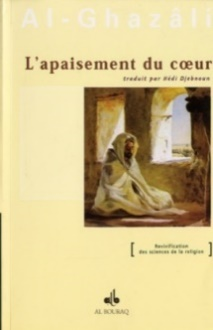
\includegraphics{Images/image002.jpg}
\sidecaption{essai}
\end{figure}


\begin{table}[h!]
\resizebox{\textwidth}{!}{%
\small
\begin{tabular}{p{2cm}p{4cm}p{4cm}}
\toprule
essai & essai & essai \\
\midrule
essai & essai & essai \\
\bottomrule

\end{tabular}%
}
\sidecaption{essai}
\end{table}

\begin{longtable}{p{6cm}p{6cm}}
\toprule
\endhead
«~Quiconque obéit au Messager obéit certainement à Allah~». 
&\TArabe{ مَّن
يُطِعِ الرَّسُولَ فَقَدْ أَطَاعَ اللَّهَ }\\
\bottomrule
\end{longtable}
%\part{Sacramentaire}



\chapter{Introduction}
%---------------------------------------------------------------------------------------------------------------

\mn{LM Chauvet}

\hypertarget{pour-se-repuxe9rer-dans-le-vaste-monde-de-la-sacramentalituxe9-lorganisme-sacramentel}{%
\section{Pour se repérer dans le vaste monde de la sacramentalité~:
l'organisme
sacramentel}\label{pour-se-repuxe9rer-dans-le-vaste-monde-de-la-sacramentalituxe9-lorganisme-sacramentel}}

\hypertarget{sacrement-un-concept-analogique}{%
\paragraph{«~Sacrement~»~: un concept
analogique}\label{sacrement-un-concept-analogique}}

\hypertarget{lorganisme-sacramentel-analyse-systuxe9mique}{%
\paragraph{l'organisme sacramentel~: analyse
systémique}\label{lorganisme-sacramentel-analyse-systuxe9mique}}

\hypertarget{une-duxe9finition-des-sacrements}{%
\paragraph{\texorpdfstring{Une définition des
sacrements}{ Une définition des sacrements}}\label{une-duxe9finition-des-sacrements}}
 

%---------------------------------------------------------------------------------------------------------------
\section{Ouverture sur la problématique
d'ensemble} 

la pointe des sacrements~: la communication de Dieu, la grâce.

«~\textbf{pour la Gloire de Dieu et le salut du monde~»}

dimension latreutique dimension sanctificatrice

Nos liturgies exercent de multiples fonctions~: cognitives, philo,
économiques~!, sociales\ldots{} quei ne doivent pas masquer
l'essentiel~: \textbf{la communication de Dieu.}

\begin{Ex}
 «~le Corps du Christ~: Amen~»

\begin{itemize}
\item
  on ne peut pas faire plus bref
\item
  de la foi
\item
  ie~: les mots «~nus
\end{itemize}

Cette nudité des mots qui se visibilise par la nudité de la main tendue,
\textbf{nue.}
\end{Ex}


Le salut de Dieu , dit dans la Parole, vient se déposer sur le corps.

Pb~: Comprendre ce que l'on célèbre~: «~Lex orendi, lex credendi~».

\paragraph{3 modèles de compréhension~:}

\hypertarget{moduxe8le-objectiviste}{%
\paragraph{Modèle objectiviste}\label{moduxe8le-objectiviste}}

St Thomas d'Aquin -\textgreater{} Trente -\textgreater{} Catéchisme de
1947\sn{«~des signes sensibles institués par Notre Seigneur Jésus
  Christ pour produire ou augmenter la grâce dans nos âmes~».}

\textbf{Sacrement comme instrument de production de la grâce~;
insistance sur la dimension de «~cause~» ou de moyen du salut.}

Dieu -\textgreater{} Sacrement -\textgreater{} Homme -\textgreater Dieu

Pb~: l'homme n'intervient pas dans le sacrement

\begin{itemize}
\item
  peu importe que l'homme «~comprenne~», pourvu qu'il soit sanctifié =
  limite)
\end{itemize}

Insistance~: Sacrement comme moyen, cause de salut

Avantage~: \textbf{souligne l'action de Dieu.}

\textbf{Instrument, canal, remède, germe.}

\hypertarget{moduxe8le-subjectiviste}{%
\paragraph{Modèle subjectiviste}\label{moduxe8le-subjectiviste}}

En réaction

Cf K. barth, qui craignait que la Liberté de Dieu soit «~compromise~»
par les sacrements, trop canalisée.

Le Baptême ne fait que \textbf{refléter} la \emph{justification et la
sanctification.} Dieu l'a déjà fait.

Contre une conception~»magique~» des sacrements.

Dieu -\textgreater{} Homme --\textgreater{} Sacrement -\textgreater{}
Dieu

\textbf{Sacrement comme instrument de traduction du déjà-là de la grâce.
Insistance sur la dimension de «~signe~» de salut (déjà donné).}

Avantage~: prend bien en compte le vécu humain. Dieu n'a jamais été lié
par les sacrements dans sa puissance de salut.

Inconvénient~: ne rend pas compte de l'efficacité du sacrement
lui-même.~: Trop exclusif.

Mais ce schéma va contre toute la \textbf{Tradition Chrétienne }(y
compris les pères).

Il est pourtant très à la mode, en réaction contre l'Église et en
insistant sur l'orthopraxie au lieu de l'orthodoxie.

\hypertarget{moduxe8le-vatican-ii}{%
\paragraph{Modèle Vatican II}\label{moduxe8le-vatican-ii}}

Schéma à «~double sens~»

Essai de tenir ensemble les dens sens (moyen de salut et signe du salut)

Dieu $\leftarrow$ $\rightarrow$ Homme $\leftarrow$ $\rightarrow$ Sacrement $\leftarrow$ $\rightarrow$ Dieu

Dieu~: \textbf{sujet opérateur des sacrements (}moyen de
salut-\textgreater{} vie humaine sanctifiée = louange à Dieu)

Difficulté~: tenir bien ensemble les deux sens

«~signe~» et «~cause~» ne sont pas des \textbf{catégories homogènes}


\paragraph{Question d'ouverture}

St Thomas d'Aquin~: II a II ae 89 prologue~; question sur l'éthique

→ on pourrait traiter ici (éthique) des sacrements → \textbf{sommet de
la vie éthique}

il aurait pu dire~: «~cause signifiante~» ou signe «~causant~».

un signe qui ne signifie que par mode de cause

une cause qui ne cause que par mode de signe

Chauvet, «~symbole et sacrement~»

Cf langage

\emph{Alliage homogène entre les deux~; grâce aux outils concernant le
\textbf{langage. }}

«~signe efficace~»~: mais c'est comme le langage~!

%-------------------------------------------------------------------------------------------------------------------------------
\section{Sacrement~: approche historique}

%-------------------------------------------------------------------------------------------------------------------------------
 
La constitution de la sacramentaire

Article LM Chauvet, «~sacrements~» dans Catholicisme

\hypertarget{mysterion-sacramentum}{%
\subsection{Mysterion -- Sacramentum}\label{mysterion-sacramentum}}

méfiance initiale contre le mot~; utilisé par les religions à mystère.

\textbf{Tertullien~;} aspect juridique~: la caution, le serment (cf
renonciation au mal)

Le Baptême comme \emph{pacte (foedus).}

La traduction en latin a fait perdre le lien avec le mysterion biblique,
l'économie divine.

Un vécu liturgique essentiel

\hypertarget{la-contreverse-sur-le-baptuxeame-des-huxe9ruxe9tiques}{%
\subsection{La contreverse sur le Baptême des
hérétiques}\label{la-contreverse-sur-le-baptuxeame-des-huxe9ruxe9tiques}}

Cyprien → Baptême lié à l'Église donc si deux Églises, deux Baptêmes .

→ Donatiste

en face Augustin~:~»le Christ agit «~etiam per malum ministrum~».

mais réception elle est fonction des dispositions personnelles.

\hypertarget{le-haut-moyen-uxe2ge}{%
\subsection{Le Haut moyen-âge}\label{le-haut-moyen-uxe2ge}}

présence réelle~: première question

\hypertarget{la-scholastique}{%
\subsection{la scholastique}\label{la-scholastique}}

la théologie comme science.

D'abord la finalité puis Importance de la causalité (Airstote)

Pratique de la LOI~: signifiait le Foi qui sauve mais ne causait pas le
salut. Signe non causal.

Importance de la pratique

Limites~:

\begin{itemize}
\item
  un schéma fondamentalement «~productionniste~»
\item
  le Cloisonnement des sept sacrements (et non les sacrements liés BEC
  cf 44)
\item
  l'absence d'ecclésiologie entre la christologie et la sacramentaire
\item
  une théologie trop en marhe de l'action liturgique
\item
\end{itemize}

\hypertarget{ouverture}{%
\section{ouverture}\label{ouverture}}

la sacramentaire scolastique est le fruit de la nouvelle
«~\emph{epistemé~»} né au 12° siècle . La fidélité à la grande tradition
théologique nous requiert non pas de reproduire mais d'en faire une
hérméneutique (décodage/recodage) nécessairement nouvelle ou sein de la
nouvelle culture qui est la notre.

 
%-------------------------------------------------------------------------------------------------------------------------------
\chapter{Sacrement de la Réconciliation}

%-------------------------------------------------------------------------------------------------------------------------------

Le «~Sacramentum~» comme langage symbolique et rituel

\hypertarget{introduction}{%
\section{Introduction}\label{introduction}}

Trilogie d'inspiration agustinienne~:

\begin{itemize}
\item
  \textbf{sacramentum -- rite- célébration --} ce qui se voit
\item
  \textbf{res sacramenti -- réalité du sacrement = la grâce}
\item
  \textbf{res et sacramentum~: 1\textsuperscript{er} effet de la grâce,}
  qui n'est pas la grâce finale ou \textbf{caractère~:}
\item
   
  ex~: on peut «~perdre~» la res sacrementi du Baptême tout en
  conservant la \emph{res et sacramentum.} (on reste baptisé).
   
\end{itemize}

Sacramentum → res sacramenti

\emph{res et sacramentum~}comme frontière

Entre le signe humain →

→ \textbf{médiation} ecclésiale ou 1\textsuperscript{ère} effet

Et la grâce de Dieu →

 %---------------------------------------------------------------------------------------
  \section{Problématique du langage} 

\begin{Synthesis}
    \begin{enumerate}
  \item
    {La langage n'est pas un instrument à la disposition de
    l'homme~; il est la médiation d'avènement du sujet c'est à dire le
    milieu dans lequel advient le sujet}
  \item
    {Puisqu'il n'est jamais de sujet hors langage (ou hors
    culture), constamment nous parlons ou «~ça parle~» en nous} \sn{Exemple~: culture où il n'y a qu'un seul mot «~s'occuper~» pour
      dire \emph{travailler} ou \emph{avoir des loisirs.} Le plus
      naturel , chez nous, est souvent le plus culturel.}

 
  \item
    {D'où la révolution épistémologique contemporaine quant à la
    manière de comprendre le rapport entre le sujet et le réel}
  \end{enumerate}
\end{Synthesis}


\textbf{Sujet} $\leftarrow$ $\rightarrow$ \textbf{Réel}

→ \emph{perception du}

\emph{← image mentale~; concept}

\begin{itemize}
\item
  \emph{restitution}
\end{itemize}

Langage

Pb de ce schéma~: il pose le langage comme instrument~: sujet =
antérieur (logiquement) au langage


\begin{Prop}
    {le concept d'~"expression" dans cette perspective~: le
  langage est simultanément «~révélateur~» et «~opérateur~»}
\end{Prop}



\textbf{Sujet} $\leftarrow$ $\rightarrow$ \textbf{Réel}

\textbf{Langage - culture}

{$\rightarrow$ \textit{le rapport au réel est toujours déjà aménagé~;} il est toujours
construit (le découpage sémantique n'est pas le même selon les cultures)
\textbf{le réel construit comme monde}}

\emph{$\leftarrow$le sujet se construit ainsi comme sujet}

Transition~:

Fonction du langage~: pas seulement utilitaire (information) mais
dimension symbolique (communication)

\hypertarget{probluxe9matique-du-symbole}{%
\section{Problématique du symbole}\label{probluxe9matique-du-symbole}}

\hypertarget{le-symbole}{%
\subsection{Le symbole}\label{le-symbole}}

Le symbole est médiateur de reconnaissance et d'alliance entre les
sujets.\sn{Cf Tertullien~; \emph{militia Christi}}

 
\paragraph{Le symbole antique}
 

Cf Tobie, 5 «~quel signe de reconnaissance donnerai-je~?~»

Triple aspect~:

\begin{itemize}
\item
  Systémique~: 1 élément n'est symbole que dans son rapport avec les
  autres éléments du même ensemble
\item
  Identitiaire~: se reconnaître comme partenaire
\item
  Juridique~: il faut être d'accor sur les \textbf{règles du jeu~.}
  Instance tierce de la Tradition, de la Loi~?
\end{itemize}
\mn{Cours du 4/2/03

Cours du //03}


Echange symbolique~: hors valeur

Intérêt théologique, grâce et échange symbolique

\hypertarget{luxe9change-symbolique}{%
\subsection{2.3 L'échange symbolique}\label{luxe9change-symbolique}}

\hypertarget{intuxe9ruxeat-thuxe9ologique}{%
\paragraph{2.32 Intérêt
théologique}\label{intuxe9ruxeat-thuxe9ologique}}

\hypertarget{b.-parole}{%
\paragraph{b. Parole}\label{b.-parole}}

Il n'y a rien de plus efficace que la parole

La parole ce n'est pas que des mots

Il suffit d'un «~je t'aime~» pour que la vie revienne

Mais aussi à travers le corps

\hypertarget{ruxe9flexion-sur-leucharistie}{%
\subparagraph{Réflexion sur
l'eucharistie}\label{ruxe9flexion-sur-leucharistie}}

Jn 6~: Pain de vie

Jésus est le pain de vie descendu du ciel

Rapport à la \emph{manne.}

\begin{itemize}
\item
  Mannu~: qu'est ce que c'est~?
\item
  On ne peut pas la stocker (ce n'est pas de la valeur)
\item
  Elle est donné quotidiennement
\item
  Sg 16~: «~elle était comme le pain des anges et elle s'adaptait au
  goût de chacun) Sg C'est vraiment du miel qu'est la sagesse
\item
  Beauchamp~: \emph{c'est le pur signe non chose}
\end{itemize}

La manne se prétait particulièrement à une analogie de la PAROLE.

1\textsuperscript{ère} tentation de la faim~: Mt 4,4 l'homme ne vit pas
seulement de pain mais de la parole qui sort de la bouche de Dieu.

\begin{itemize}
\item
  Dieu donne la manne pour que l'homme comprenne que la parole fait
  vivre (ref à Dt 8~?)
\item
  Pour manger l'eucharistie, il faut avoir ruminer la parole (cf
  élévation de la Bible et élévation de l'eucharistie)
\item
  Christ se présente comme la parole de vie envoyé par Dieu. Jn comprend
  la manducation d'eucharistie est une rumination de la parole douce et
  amère d'un Christ qui se livre pour la vie du monde.
\end{itemize}

L'expérience anthropologique de manger physiquement la parole pour
qu'elle soit complétement entendu~: d'où l'eucharistie~: parole donnée
sous le mode sacramentel

La Parole, c'est le Christ

\begin{itemize}
\item
  2 Co 10~: Le Christ est le OUI de Dieu au monde.
\end{itemize}

\hypertarget{eviter-le-piuxe8ge-de-la-chosification}{%
\subparagraph{Eviter le piège de la
chosification}\label{eviter-le-piuxe8ge-de-la-chosification}}

L'échange symbolique permet de ne pas chosifier ni magnifier (S Thomas
n'avait pas cet outil conceptuel~: dommage~!)

\hypertarget{c.-gratuituxe9}{%
\paragraph{Gratuité}\label{c.-gratuituxe9}}

\textbf{Charis}~: la grâce, ce qui est gratuit

Deux sens~:

\begin{itemize}
\item
  gratis Data~: donné gratuitement
\item
  \emph{gratiam gratum~:} gracieuseté. celle qui nous rend gracieux aux
  yeux de Dieu. Père de l'Eglise.
\end{itemize}

D'une part la grâce est gratuite~: elle ne dépend pas de nos mérites.

MAIS cela ne veut pas dire qu'il n'y ait pas de CONTRE DON, car sinon,
Dieu nous traiterait comme un OBJET (ALIENATION~: nous serions alors
écrasés). Or, il nous traite comme un SUJET. \emph{Un DON oblige.} Ce
n'est pas la \emph{conséquence} mais la \emph{marque} du don, car sinon
ce n'est pas un don car il n'est pas reconnu par la personne qui le
reçoit.

DON RECEPTION CONTRE-DON

Quand nous rendons grâce à Dieu pour les dons, nous ne sommes pas dans
le marchandage.

\hypertarget{baptuxeame-des-petits-enfants}{%
\subparagraph{Baptême des petits
enfants}\label{baptuxeame-des-petits-enfants}}

Le plus bel exemple de la gratuité de la grâce~: il ne tient pas compte
des mérites et démérites pour nous sauver. Mais il renforce un schème de
concurrence entre Dieu et l'Homme. Car le contre-don n'est pas marqué.
D'où l'importance de penser le baptême des petits enfants comme un
dérivé des adultes~: ACTE LIBRE~; êtres responsables.

\hypertarget{d.-le-thuxe9ologal-dans-lanthropologique}{%
\paragraph{le théologal dans
l'anthropologique}\label{d.-le-thuxe9ologal-dans-lanthropologique}}

échange symbolique pour approcher le mystère de la rencontre entre Dieu
et l'homme dans les Sacrements (leur efficacité)

\begin{itemize}
\item
  pas une simple analogie~: c'est la STRUCTURE dans laquelle s'effectue
  cette échange
\item
  le théologal se joue dans l'anthropologal, dans la constitution de
  l'homme
\end{itemize}

\hypertarget{lacte-de-symbolisation-analyse-et-application-uxe0-leucharistie}{%
\subsection{L'acte de symbolisation~: analyse et application à
l'eucharistie}\label{lacte-de-symbolisation-analyse-et-application-uxe0-leucharistie}}

2 agents secrets, avec billet de banque~déchiré; acte de symbolisation
pour se reconnaître partenaire

caractéristique

\begin{itemize}
\item
  systémique
\item
  symbolique
\item
  juridique (il faut avoir défini préalablement que le billet était le
  code de rencontre)
\end{itemize}

 

\begin{table}[h!]
    \centering
    \sidecaption{articuler  }
 
\begin{tabular}{p{.2\textwidth}p{.2\textwidth}p{.2\textwidth}}
\toprule
Christ &$\leftarrow$ $\rightarrow$ & Eglise \\
 
\\
\bottomrule
\end{tabular}
\label{tab:my_label}
\end{table}

 

 
\begin{table}[h!]
    \centering
\sidecaption{Des éléments du même ensemble mais qui sont
différents  }
 
\begin{tabular}{p{.2\textwidth}p{.2\textwidth}p{.2\textwidth}}
\toprule
Christ &($\leftarrow$ $\rightarrow$) & Eglise \\
 
\\
\bottomrule
\end{tabular}
\label{tab:my_label}
\end{table}


 

Ex~: un signe de Croix chez les papous~: ils ne peuvent pas le rattacher
aux autres éléments~: FONCTIONNEMENT imaginaire

\begin{table}[h!]
    \centering
\sidecaption{Chaque élément ne tient sa pertinence symbolique que de
par le rapport qu'il entretient avec les autres éléments de
l'ensemble
Le Christ n'existe que par l'Eglise dans le sens que sans Eglise,
personne ne connaîtrait le Christ }
\begin{tabular}{p{.2\textwidth}p{.2\textwidth}p{.2\textwidth}}
\toprule
Christ &$\leftarrow$& Eglise \\
        &   $\rightarrow$ \\
\\
\bottomrule
\end{tabular}
\label{tab:my_label}
\end{table}


\hypertarget{eucharistie}{%
\subparagraph{Eucharistie}\label{eucharistie}}

1Co 11~: Paul reproche au Co de prendre le repas du Seigneur

\begin{enumerate}
\def\labelenumi{\arabic{enumi}.}
\item
  niveau \emph{ecclésiologique et Ethique}~: vous prétendez prendre le
  repas alors que votrer pratique est en contradiction
\item
  niveau sacramentaire~ ou plutôt liturgique : Paul raconte le récit de
  la cène~: iatus entre la réponse et le problème posé
\item
  donc «~discernez le corps~». Le problème des Co, ce n'est pas la
  transsubstantiation\sn{Question apparue au IXème\ldots{}} (pas
  un problème sur la présence réélle). Mais mettre en rapport les
  membres du corps du Christ avec le corps Sacramentel (1 et 2)
\end{enumerate}

\hypertarget{rite-de-communion}{%
\subparagraph{Rite de Communion}\label{rite-de-communion}}

Lex Orandi, Lex Credendi

Regarder comment se pratique la célébration

\begin{table}[h!]
    \centering
      \sidecaption{ }
 
\begin{tabular}{p{.2\textwidth}p{.4\textwidth}}
\toprule
Geste de paix & «~Donnez-vous la paix~»~: ce qui est premier, c'est le
rapport horizontal avec mes frères \\
Fraction de paix & Rapport vertical (le Christ) pour faire l'unité des
membres de son corps (horizontal) \\
Démarche de Communion & Rapport vertical \\
\\
\bottomrule
\end{tabular}
\label{tab:my_label}
\end{table}
 

On ne peut pas séparer l'Eglise du Christ

\hypertarget{huxe9ruxe9sie-de-buxe9renger-de-tours}{%
\subparagraph{Hérésie de Bérenger de
Tours}\label{huxe9ruxe9sie-de-buxe9renger-de-tours}}

XIème 1053

Hérésie sur la présence du Christ dans l'eucharistie

Pb~: on n'a pas les outils conceptuels pour penser cette présence du
Christ. On pensait une adhérence du Christ aux espèces, qu'on aurait dû
le voir. Seulement par un deuxième miracle, Dieu étant un voile qui nous
le cache, afin que nous fassions un acte de foi (Isidore de Seville).

Il a fallu attendre le XII, pour que l'on trouve le concept adéquat,
celui de SUBSTANCE aristotélicien (on ne voit que les Accidents).

Les trois corps sont liés~:

\begin{enumerate}
\def\labelenumi{\arabic{enumi}.}
\item
  Corps historique et glorieux
\item
  Corps mystique sacramentel
\item
  Corps écclésial
\end{enumerate}

2---3~: Soyez ce que vous voyez~; recevez ce que vous êtes. Aug.
\sn{A lire sur S. Augustin~: Chair\ldots, Chair de l'Eglise Tillard}

Corpus Verum~était devenu le Corps ecclésial (H. de Lubac). Mais
berenger diminue le lien entre 1 et 2. En réaction, on a renforcé 1 et 2
au détriment de 2 et 3. L'adoration du Christ dans l'Eucharistie est
devenue plus importante que la Communion.\sn{\textbf{Historique}~:

  Pratique de la communion annuelle

  La réserve eucharistique (pour les malades) se formalise

  Evolution d'une conception de l'eucharistie action vers l'eucharistie
  chose (ex~: Transubstanciation en réaction contre l'hérésie de
  bérenger de Tours, qui utilise le concept aristotélicien de substance
  XII).

  Développement des processions, XIII «~le peuple n'a plus faim du pain
  eucharistique, rassasié des processions~».

  Elévation~: telle importance que l'on en attend de merveilleux effets
  deprotection contre les malheurs ou de vision miraculeuse du Christ
  lui même
  Exposition du Saint Sacrement dans une monstance lors de la
  contre-réforme}

\hypertarget{quimporte-la-valeur-de-luxe9luxe9ment-symbolique}{%
\paragraph{Qu'importe la valeur de l'élément
symbolique}\label{quimporte-la-valeur-de-luxe9luxe9ment-symbolique}}

Le symbole ne fonctionne pas à la valeur~: Crucifix~: bout de bois~;
bague de fiançailles

Musique~: ky-ri-e suffit -- pas besoin de 10 Mn de kyrie de
Mozart\ldots{}

\hypertarget{le-laboureur-et-ses-enfants-de-la-fontaine}{%
\subparagraph{«~Le laboureur et ses enfants~» de la
Fontaine}\label{le-laboureur-et-ses-enfants-de-la-fontaine}}

\begin{itemize}
\item
  Gardez-vous de vendre l'héritage, il y a un grand trésor dedans
\item
  ils labourent le champ
\item
  le travail est le trésor
\end{itemize}

Analogie intéressante avec le sacrement~:

\begin{itemize}
\item
  le sacrement n'est pas un trésor dans le champ
\item
  J'en suis obligé Grammaticalement~: la grâce est posé comme Objet
\item
  SUJET -- VERBE -- OBJET~: Dieu Donne la Grâce
\item
  Penser en théologie comme en philosophie, c'est apprendre à se défaire
  de son discours.
\item
  Heiddegger casse le langage~; Lévinas. Contre réduction
  phénoménologique. Risque certes de préciosité. Mais il faut casser les
  représentations.
\item
  La grâce n'est pas un objet valeur, même spirituel
\item
\item
  nous sommes la terre labourée. DurchArbeitung de Freud~: nous sommes
  travaillés
\item
  le socle de la charrue, c'est la parole de Dieu qui nous advient sous
  le mode rituel
\item
  il faut une force de traction, c'est l'ES
\item
  Nous allons nous transformer en acteur d'Alliance, alors que nous
  sommes tous héritier de Cain.
\item
  Cet engendrement permanent de nous même, nous devenons un peu plus
  fils de Dieu.
\end{itemize}

\begin{Def}[Grâce]
 un «~se recevoir~» toujours en cours
\end{Def}
  

\hypertarget{lacte-de-symbolisation-est-simultanuxe9ment-ruxe9vuxe9lateur-et-opuxe9rateur}{%
\paragraph{L'acte de symbolisation est simultanément révélateur et
«~opérateur~»}\label{lacte-de-symbolisation-est-simultanuxe9ment-ruxe9vuxe9lateur-et-opuxe9rateur}}

Le billet est à la fois «~révélateur~»~: ils se reconnaissent équipiers
mais aussi «~opérateur~»~: ils sont liés jusqu'à la mort dans leur
projet.

\hypertarget{doxologie}{%
\subparagraph{Doxologie}\label{doxologie}}

Par lui, avec lui et en lui

On présente à dieu , conjoint la terre au Ciel.

La voix monte aussi vers Dieu ainsi que les bras. Mais ce que nous
montons, c'est le Christ.

Puissance incroyable

Le Chrétien~: se reconnaît à Dieu, pour Dieu, en Christ.

C'est à force de faire des gestes comme cela que l'on devient Chrétien
et de les faire en Eglise. Attention à ne pas le psychologiser.

Une Foi ne vit qu'en se MANIFESTANT. Si on ne le dit jamais, notre foi
est quasiment morte.

\hypertarget{quelques-lois-de-la-ritualituxe9}{%
\section{Quelques lois de la
ritualité}\label{quelques-lois-de-la-ritualituxe9}}

\hypertarget{un-jeu-de-langage-original}{%
\subsection{Un «~jeu de langage~»
original}\label{un-jeu-de-langage-original}}

Ex~: génocide du Rwanda

\begin{itemize}
\item
  type \textbf{exactitude}~: discours du politologue
\item
  type témoignage~: discours du témoin~: reconstruit l'évenement pour ce
  faire comprendre. \textbf{Vérité narrative ou herméneutique}
\item
  type poétique~: vérité \textbf{poétique.} On ouvre un monde possible
  (Ricoeur)
\item
  Les trois types de langages visent la vérité de différentes voies.
\end{itemize}

Différents langages de ritualité~:

\begin{itemize}
\item
  théologique
\item
  mystique~: métaphore, affects (S. jean de La Croix)
\item
  témoignage~: MCC. On se raconte.
\item
  rituel
\end{itemize}

Attention, à ne pas se tromper de registres~: respecter les jeux de
langage différents. Ex~: à la messe, on ne parle pas de la théologie du
péché originel.

La liturgie croule sur les demandes contradictoires. Elle est faite pour
que l'on puisse recevoir le don de Dieu. Elle ne permet pas tout.

\hypertarget{lecture-thuxe9ologique-de-quelques-caractuxe9ristiques-majeures-de-lexpression-rituelle}{%
\subsection{Lecture théologique de quelques caractéristiques
majeures de l'expression
rituelle}\label{lecture-thuxe9ologique-de-quelques-caractuxe9ristiques-majeures-de-lexpression-rituelle}}

\hypertarget{un-langage-pragmatique-langage-action}{%
\paragraph{3.21 Un langage pragmatique~: langage
--action}\label{un-langage-pragmatique-langage-action}}

c'est une «~URGIE~» - ergon~: action\sn{Siderurgie,
  chirurgie,\ldots{}}

de l'ordre de la communication symbolique. Ne s'indresse pas à
l'intellect (non pas un LOGOS\sn{théologie,}) mais à tout le
corps. Lieu de jouissance~: on a une rencontre avec le Dieu Bon (et non
pas le Dieu Vrai\ldots).

\begin{itemize}
\item
  mon âme a soif de Dieu
\end{itemize}

\hypertarget{cuxe9luxe9bration-pour-les-enfants}{%
\subparagraph{Célébration pour les
enfants}\label{cuxe9luxe9bration-pour-les-enfants}}

But~: leur laisser 5 mn avec Dieu

\hypertarget{cest-la-muxe9moire}{%
\subparagraph{C'est la mémoire}\label{cest-la-muxe9moire}}

La liturgie, c'est une mémoire~: les places sont en attente\ldots{} Même
les gestes,

La faiblesse de Croire, Michel de Certeau

\textbf{Faites ce que vous dites~}: ex~: soyez dans la joie = chanter.
Ex~: onction au Baptême~: pas besoin d'expliquer~: cela sent bon,
imprègne le front.

\mn{Cours du 7/03/02}

\hypertarget{petite-lecture-thuxe9ologique}{%
\paragraph{Petite lecture
théologique}\label{petite-lecture-thuxe9ologique}}

Notion de \textbf{parole}~: sens d'Action en hebreu

\begin{itemize}
\item
  pas le logos grec
\item
  le DABAR (traduire par  dans la LXX)
\item
  SACREMENT, déploiement de ce qu'est le DABAR, la parole
\end{itemize}



    \paragraph{Un langage symbolique, donc économique~: sobriété et
    «~réserve~» du
    rite}

Symbole~: il rend PRESENT la chose (cf le drapeau brulé)~: il EST et il
n'EST pas le réel qu'il représente.

Les symboles représentent des mondes

Le symbole est \textbf{sobre.} Un peu suffit. Ex~: \emph{donnons-nous un
signe de paix~: ainsi nous nous engageons à nous réconcilier~; pas
besoin de faire le tour de l'Eglise.} Un peu de vin, un peu d'eau. Il ne
faut jamais substituer le réel au symbole.

Donner la chance au symbole~: ne pas tout expliquer~: on s'est trompé de
registre.

Goupillon~: moyen age~: préférer du buis.

Attention à la dérive \textbf{festive.} Injonction~: «~quand il
\emph{faut} faire la fête, ce n'est pas drôle\ldots~». Elle peut surtout
faire obstacle au passage de la mort vers la vie à faire avec le Christ.

Geneviève Hébert, Eloge \emph{de la pudeur en matière de dévotion et
ailleurs}, MD 215-225

LM Chauvet, \emph{Eschatologie et Sacrement}, MD 220\\
nos symboles liturgiques sont sobres. Elle est la médiation de la
condition eschatologique dans laquelle nous sommes~: le salut est déjà
donné mais pas encore achevé. Nous chantons «~\emph{Alleluia}~» car déjà
là mais nous ne nous laissons pas entraîner car tout n'est pas déjà
acquis~: cela peut être une insulte à tous les gens qui souffrent depuis
2000 ans~: RESERVE eschatologique.

J. CAILLOT, \emph{Liturgie et eschatologie,} MD 220

Grande originalité. Puisque le salut est déjà venu, il faut nous donner
sans réserve dans les tâches éthiques. Mais puisqu'il n'est pas complet,
toujours donné à Dieu le dernier mot.

JB METZ~: RESERVE~:tout pouvoir politique est réservé à Dieu.

Ici différent, «~PAS de JUBILATIO sans MODERATIO~» Augustin.

Expression de \textbf{Sainte Réserve.} Ce morceau de pain est un peu
dérisoire mais nous faisons une genouflexion~: nous prenons acte du
salut déjà donné mais nous le faisons devant un symbole tellement
dérisoire, qu'il indique que ce salut n'est pas achevé.

VERTUS DE LA PHENOMENOLOGIE en théologie.

Isabelle XXXX, \emph{Les actes de langage dans la prière} LMD 196

S'inspire de PEIRCE, entre un représentant (prêtre) et un représenté (le
Christ), il y a quatre relations possibles~:

\begin{itemize}
\item
  ICONE, de type photographique\sn{cf Critique de Theissen de la
    lecture iconique des sacrements, vision protestante, \emph{La
    religion des premiers chrétiens}}
\item
  Relation de DIAGRAMME (MODELE)
\item
  Relation de l'INDICE, de la GIROUETTE par rapport au VENT~: il y a un
  contact mais pas de ressemblance.
\item
  Rapport SYMBOLIQUE\sn{attention, pas le sens donné précédemment},
  entre un signifiant et signifié dans une langue (ex~: HORSE = cheval).
\end{itemize}

Ex~: Centurion, «~je ne suis pas digne~»~:

\begin{itemize}
\item
  je suis le centurion (ICONE)
\item
  je dis cela parce que l'on m'a demandé (SYMBOLIQUE)
\end{itemize}

un jeu possible entre les différents possibles~: chacun peut faire jouer
différemment le rituel, qui respecte chacun. Parfois, nous serons le
centurion. En liturgie, \textbf{Le moi est en état de recomposition.}

P°108

Rapport du prêtre au Christ~: ICONE, DIAGRAMME, INDICE, les trois sont
possibles en théologie catholique mais probablement pas SYMBOLIQUE
(vision protestante)~:

\begin{itemize}
\item
  la représentation ICONE est inadaptée à l'ordination de femme mais les
  deux autres.
\item
  A creuser
\end{itemize}

\hypertarget{un-langage-huxe9tuxe9rotopique-qui-reluxe8ve-dun-autre-lieu-que-le-quotidien-lordinaire-lutilitaire}{%
\paragraph{un langage «~hétérotopique~», qui relève d'un autre
lieu que le quotidien, l'ordinaire,
l'utilitaire}\label{un-langage-huxe9tuxe9rotopique-qui-reluxe8ve-dun-autre-lieu-que-le-quotidien-lordinaire-lutilitaire}}

kyrie 3 fois, étole, position du corps

il reste donc une distance entre la langue du rituel et la langue
vernaculaire.

\begin{itemize}
\item
  cela permet de comprendre pourquoi le Latin a aussi duré aussi
  longtemps
\item
  «~Cela est juste et Bon~»~: plutôt qu'on le «~ratifie~».
\end{itemize}

Fonctionnalité esthétique

Deux dérives possibles~: il faut que ce soit simple à prendre (verre) et
une dérive esthétisante (le bel objet)

TOUJOURS une rupture SYMBOLIQUE dans une célébration liturgique.

\begin{itemize}
\item
  rompt avec l'utilitarisme
\item
  crée un espace de gratuité dans lequel Dieu va pouvoir advenir
\end{itemize}

\hypertarget{un-langage-programmuxe9-et-donc-ruxe9ituxe9rable}{%
\paragraph{Un langage programmé (et donc
réitérable)}\label{un-langage-programmuxe9-et-donc-ruxe9ituxe9rable}}

On reçoit un rite. Le rite est codé (ex~: comment rentrons nous dans une
salle de cours). Cela permet d'économiser de l'énergie.

Il est reçu de générations antérieures, avec un Ancêtre. Le langage
courant le dit~: «~est rituel, ce qui est habituel~». Programme qui est
reçu.

Cette programmation n'est pas sans ambiguité~: une routine.

En particulier, les jeunes s'ennuient très vite. NEW -- LIVE -- SHOW.
Or, la liturgie , c'est exactement l'inverse.

Pourtant, cette programmation est protectrice de liberté. Ex~:
\emph{quand nous prenons congé après un diner, nous executons le rite.
Mais ce rite peut être chaleureux ou non.}

Il faut accepter de jouer le jeu du code mais il y a une manière
d'habiter le code.

facteur de liberté. Cela m'empêche de me demander ce que je dois faire.

Possiblement libérateur.

\hypertarget{valeur-thuxe9ologique}{%
\paragraph{Valeur théologique}\label{valeur-thuxe9ologique}}

Double valeur théologique~:

\begin{itemize}
\item
  \textbf{Christologique}~: institution de l'eucharistie~: rien n'est
  plus programmé~: les 4 verbes de cette institution (prendre, bénir,
  rompre, donner) servent à structurer l'eucharistie. Confession de foi
  de l'Eglise par mode de faire symbolique, que le Christ est SEIGNEUR~:
  le faire parce qu'il a dit de le faire. (approche phénoménologique~:
  je regarde la chose et je pense ce qui ce passe)~;
  Métaphore\sn{renvoie}
\item
  \textbf{Ecclésiologique~:} Manifester que toute célébration est
  manifestation de l'Eglise. Métonimie\sn{la partie pour le tout}.
  \emph{Quand on célébre en Afrique, on manifeste l'Eglise entière.}
  Elle n'appartient à personne. Certes particularité de la célébration
  mais pas particularisme. C'est ce que nous rappelle la programmation
  rituelle.
\end{itemize}

\hypertarget{evanguxe9liser-la-ritualituxe9}{%
\subsection{Evangéliser la
ritualité}\label{evanguxe9liser-la-ritualituxe9}}

Rite meilleur et pire.

Pire~:

\begin{itemize}
\item
  Routine, compulsion de répétition
\item
  sacralisation du politique (cf te deum)
\item
  ambiguité spirituelle~: substituer la magie du rite à la question
  existentielle de Dieu~: les protestants y sont très sensibles~:
  PRIORITE de la PAROLE.
\end{itemize}

La ritualité est toujours à evangéliser~: le rite ne devient SACREMENT
qu'avec la PAROLE et l'ESPRIT SAINT. Mais cette parole ne nous parvient
que sous mode rituelle.

%-------------------------------------------------------------------------------------------------------------------------------
\chapter{Place et fonction des sacrements dans la structure de l'Identité
Chrétienne}

%-------------------------------------------------------------------------------------------------------------------------------
 


\hypertarget{i.-introduction}{%
\section{Introduction}\label{i.-introduction}}

Se rappeler que les sacrements ne sont pas le TOUT de l'existence
chrétienne

\hypertarget{lc-24-les-disciples-demmaus}{%
\subsection{Lc 24, les disciples
d'Emmaus}\label{lc-24-les-disciples-demmaus}}

Catéchèse du passage de la non foi à la foi, de la méconnaissance à la
reconnaissance. La question qui guide ce texte, s'il est vrai que le Ch
est ressuscité, pourquoi ne pouvons-nous pas le VOIR~? Immédiatement

Comment se fait il que nous ne puissions pas le PROUVER~? question des
destinataires de Lc

Lc répond~: Renoncer à VOIR, TOUCHER, TROUVER, à leur immédiaté. Ces
verbes ne sont appliqués que sur le Cadavre du Christ. Le verbe
«~TOUCHER~» dans la 3\textsuperscript{ème} séquence~: toucher les
marques de sa mort. Si l'on veut reconnaître le Christ vivant, il faut
renoncer à cette vision de Christ Cadavre.

La transformation des deux disciples est rendue possible par~3 éléments
successifs~:

\begin{itemize}
\item
  \textbf{le rapport aux écritures,} le déblocage commence quand le
  Christ prend la parole~: «~il leur expliqua tout ce qui le concernait
  dans les Ecritures. Kerygme. \emph{Dihermeneusein}. En filigrane de ce
  que fait Jésus, il y a l'Eglise~: lecture de la thora et des
  prophètes.\\
  Technique rabbinique~: on rapprochait un élément des textes lus d'un
  autre texte, d'un élément de la tradition orale pour l'actualiser.
  Plus d'importance chez les Chrétiens pour les prophètes que pour
  Moïse.\sn{une des raisons de la rupture avec les juifs}
  Désormais, toutes les Ecritures seront interprétées par la mort et la
  résurrection du Christ . Il y a 50 ans de pratique ecclésiale. A
  chaque fois que nous relisons les Ecritures et les interprétons sous
  la lumière de Pâque, alors le Christ est présent au milieu de nous
  (\emph{Christ vivant}). \textbf{Apprendre à reconnaître le Christ dans
  l'Eglise.} «~Acclamons la parole de Dieu -- Louange à toi, Seigneur
  Jésus~».
\item
  \textbf{la fraction du pain}, au repos, à table. Il rompit le pain. 4
  verbes du récit de l'institution. il y a 50 ans de pratique
  eucharistique. Renoncer à Voir Jésus directement \textbf{mais
  apprendre à le reconnaître dans l'Eucharistie}. C'est lui qui bénit le
  pain, le rompt pour nous et nous le donne. Alors, il disparaît~: les
  yeux des disciples s'~ouvrent sur du vide, mais sur du vide plein.
  \emph{Anastantes~}: ils se lèvent (résurrection). On ne peut pas
  reconnaître Jésus sans être nous même relevés. Ils retournent alors à
  Jérusalem~: ils commencent par accueillir le témoignage des 11. C'est
  après qu'ils joignent leur témoignage. (synectode~: la partie pour le
  tout~: la bénédiction qui ouvrait le repas signifiant la totalité du
  repas).
\item
  \textbf{conduite éthique}, moins évident. Je déborde le texte pour
  aller voir les sommaires (Ac 2~; 4).Lc croque le portrait de la
  première communauté de Jérusalem~: fraction du pain, communion,
  partage fraternel, didascalie. Il insiste sur le \textbf{partage
  fraternel.} Grâce à ce partage, il n'y a plus de frères démunis. De ce
  fait, c'est le signe de la communauté eschatologique~: témoignage
  rendu à la résurrection~: «~voyez comme ils s'aiment~».\sn{J.
    DUPONT} Rappelle la théologie du 4\textsuperscript{ème} évangile.
  Comparaison en COMME~: «~la table est jaune comme le mur «~ (OS) et
  «~je suis chauve comme mon père~» (KATHOS)~: il y a participation. Cf
  lavement des pieds~: Kathos. Participation à ce qu'il fait. Quand les
  frères «~se lavent les pieds~», Jésus continue son œuvre à travers
  eux. Tertullien~: «~Le sacrement du frère~». «~tu as vu ton frère, tu
  as vu ton Dieu~» Clément d'Alexandrie.
\end{itemize}

\hypertarget{la-muxe9diation-de-leglise}{%
\subsection{La médiation de
l'Eglise}\label{la-muxe9diation-de-leglise}}

\hypertarget{schuxe9ma}{%
\paragraph{Schéma~:}\label{schuxe9ma}}

Pas de rapport direct entre nous et le Christ~: il faut passer par
l'Eglise.

Christ

Le cercle,

L'Eglise

Il n'y a pas de Chrétiens en dehors de l'Eglise. En dehors de l`Eglise,
point de salut confessé.

P. Lieger, op, \emph{l'être ensemble des Chrétiens}

L'Evangile est source d'un a priori communautaire. E\^{}tre chrétien,
c'est être d'emblée mis ensemble. Nous sommes sous sa Seigneurie tous.

Paul

\begin{itemize}
\item
   
  Col 3,9-11,
   
\item
   
  1 Co 12, 13~;
   
\item
   
  Ga 3, 26-28
   
\end{itemize}

Le baptême, c'est la réalisation du salut eschatologique~: «~il n'y a ni
juif ni grec, ni homme ni femme~».

Ep 2, 14 ss Christ est mort pour abolir le mur de séparation~; il a tué
la haine. Le juif et le grec

Ep 3~: juifs et paiens héritiers du même héritage

Yves de Montcheuil, mort en 1944 dans le Maquis, \emph{Aspects de
l'Eglise}

\emph{«~ce ne sont pas les chrétiens qui en se réunissant forment
l'Eglise, c'est l'Eglise qui fait les Chrétiens~».}

Devenir Chrétien, c'est apprendre à aimer l'Eglise peu à peu.

Cette priorité de l'Eglise.

\hypertarget{la-priorituxe9-du-nous-eccluxe9sial.-remarque-sur-la-pruxe9sidence-par-un-ministuxe8re-ordonnuxe9}{%
\paragraph{La priorité du «~nous~» ecclésial. Remarque sur la
présidence par un ministère
ordonné}\label{la-priorituxe9-du-nous-eccluxe9sial.-remarque-sur-la-pruxe9sidence-par-un-ministuxe8re-ordonnuxe9}}



\hypertarget{eglise-et-assembluxe9e-cuxe9luxe9brante}{%
\paragraph{Eglise et assemblée
célébrante}\label{eglise-et-assembluxe9e-cuxe9luxe9brante}}

\hypertarget{lassembluxe9e-dominicale}{%
\paragraph{L'assemblée
dominicale}\label{lassembluxe9e-dominicale}}

\hypertarget{ouverture-pastorale}{%
\paragraph{Ouverture pastorale}\label{ouverture-pastorale}}

\hypertarget{laccuxe8s-uxe0-la-foi-comme-consentement-uxe0-une-perte}{%
\subsection{L'accès à la foi comme consentement à une
perte}\label{laccuxe8s-uxe0-la-foi-comme-consentement-uxe0-une-perte}}

\hypertarget{triple-tentation}{%
\paragraph{Triple tentation}\label{triple-tentation}}

\hypertarget{la-bonne-santuxe9-e-la-foi}{%
\paragraph{La bonne santé de la
Foi}\label{la-bonne-santuxe9-e-la-foi}}

%---------------------------------------------------------------------------------------------------
\hypertarget{ii.-fonctionnement-de-la-structure}{%
\section{ Fonctionnement de la
structure}\label{ii.-fonctionnement-de-la-structure}}

\hypertarget{la-priuxe8re-eucharistique}{%
\subsection{1. la prière
eucharistique}\label{la-priuxe8re-eucharistique}}
 
  \paragraph{Analyse narrative}\label{analyse-narrative} 
  \paragraph{Statut du récit de l'institution~: récit de
  l'Eglise} 
  
  \paragraph{le discours
  d'anamnèse} 
 
  \paragraph{Le discours d'Epiclèse  } 
  \paragraph{Schéma du procès
  d~«~eucharisticité~»} 

\hypertarget{remarque-sur-ce-procuxe8s}{%
\paragraph{Remarque sur ce
procès}\label{remarque-sur-ce-procuxe8s}}

\hypertarget{a.-un-moduxe8le-et-non-pas-du-pruxeat-uxe0-porter}{%
\subparagraph{un modèle et non pas du prêt à
porter}\label{a.-un-moduxe8le-et-non-pas-du-pruxeat-uxe0-porter}}

La structure mentionnée la fois dernière est un patron. Le mouvement ne
commence pas nécessairement par l'Ecriture (don), cela peut être une
célébration (récéption) ou un témoignage éthique. (contre don).

Si c'est l'Evangile qui vous fait agir\ldots~? qu'y a t-il donc dans
l'Evangile~?

Le déclencheur peut être l'un des éléments, l'histoire commence
lorsqu'on ouvre l'Ecriture.

Il n'est pas d'itinéraire chrétien hors du processus Ecriture Sacrement
Ethique, vu pour la prière eucharistique.

\hypertarget{b.-le-don-duxe9pend-de-dieu-seul-mais-la-ruxe9ception-de-ce-don-comme-tel-duxe9pend-du-contre-don.}{%
\subparagraph{Le don dépend de Dieu seul~; mais la réception de ce don
comme tel dépend du contre
don.}\label{b.-le-don-duxe9pend-de-dieu-seul-mais-la-ruxe9ception-de-ce-don-comme-tel-duxe9pend-du-contre-don.}}

Dieu a l'initiative du don~! (hors dépendance de l'attitude éthique de
l'être humain) Mais il n'est de don reçu qu'avec le contre don éthique
(conversion du cœur, foi, agapè).

Validité et fécondité~:

Validité~: dépend de l'action de Dieu (et pas du sujet)

En revanche la fécondité dépend de notre cœur~: si notre vie ne s'ouvre
pas à la grâce

Un sacrement peut être valide et être reçu pour notre condamnation~! (1
Co 11).

Cf. St Augustin (controverse avec les donatistes~: leurs sacrements sont
valides «~vrais~» mais inféconds, car ils sont hors de l'Eglise.

Ne dites pas que la grâce de Dieu dépend de notre foi à l'oral~!

\hypertarget{c.-toute-cuxe9luxe9bration-sacramentelle-fonctionne-selon-ce-moduxe8le}{%
\subparagraph{toute célébration sacramentelle fonctionne selon ce
modèle}\label{c.-toute-cuxe9luxe9bration-sacramentelle-fonctionne-selon-ce-moduxe8le}}

les exemples ne manquent pas. (Ecriture et Sacrement OK, éthique =
envoi~! Peu développé à la messe, mais davantage pour un mariage)

Les sacrements ne sont pas autre chose que la cristallisation de la
Parole de Dieu.

\subparagraph{le moment sacrement~: ni point de départ,
ni point d'arrivée. Ce n'est qu'un point de passage. Mais il
{est} point de passage obligé et
obligeant} 

le moment réception n'est pas départ (ce sont les \textbf{Ecritures}) ni
arrivée (\textbf{vie chrétienne éthique})

point de passage obligeant~: car toute réception d'un don comme don
oblige~! (reconnaissance, foi, éthique de réponse)

point de passage obligé~: pour que l'éthique soit proprement chrétienne,
il faut qu'elle soit vécue comme un éthique de réponse au don premier de
Dieu (éthique théologale). Ainsi, la sanctification par le don de Dieu
est en ce sens «~obligé~». L'éthique devient elle même une liturgie, un
sacrifice spirituel. (cf prochain cours)

\hypertarget{identituxe9-juive-et-identituxe9-chruxe9tienne}{%
\paragraph{Identité juive et identité
chrétienne}\label{identituxe9-juive-et-identituxe9-chruxe9tienne}}

\hypertarget{place-du-moment-sacrement-par-rapport-au-moment-ecriture}{%
\subsection{Place du moment Sacrement par rapport au moment
Ecriture}\label{place-du-moment-sacrement-par-rapport-au-moment-ecriture}}

\hypertarget{les-ecritures-sacrement-de-la-parole}{%
\paragraph{Les Ecritures sacrement de la
Parole}\label{les-ecritures-sacrement-de-la-parole}}

Le premier «~tabernacle~» de la Parole de Dieu, les premiers sacrements
(mysteria) ce sont les Ecritures, pour les pères~!

Augustin~: sacramentum, c'est à dire n'importe quelle parole des saintes
lettres~!

N'importe quel épisode de l'Ecriture est traité comme un sacramentum~:
révélation en figure du dessein de salut de Dieu.

Pas étonnant que le livre des Ecritures ait fait l'objet d'une véritable
vénération dans la liturgie (ex~: évangéliaire)

Cf. Origène, SC7 p. 211 homélie sur la genèse. (écriture traitée avec
autant de poids que l'eucharistie). Voir aussi SC16 p. 263 homélie sur
exode

Ainsi l'Evangéliaire est orné, on l'encense, on chante alléluia\ldots{}
Voire procession~: Dei Verbum~21 : une seule table aussi bien de la
Parole que du Corps du Christ, et une seule vénération.

L'expression de «~pain de vie~» est aussi bien employée pour la parole
de Dieu que pour l'Eucharistie~! Il faut retrouver le réflexe de penser
au pain de vie comme étant d'emblée la Parole~!

(si on avait le temps, la sacramentaire devrait inclure les icônes)

Livre tabernacle -- sacrement de la Parole de Dieu

Il existe une tentation de dire que la Parole de Dieu est l'Ecriture
interprétée. NON C'est l'Ecriture dans sa lettre~! (cf. Parler
d'Ecriture Saintes~: prise en compte de la lettre dans la positivité
historique, son altérité culturelle, comme sacramentum). L'esprit n'est
trouvé que si la lettre n'est pas esquivée. C'est pareil pour la
sacramentaire.

On peut craindre qu'à force d'encenser le livre, on idôlatre la lettre~:
il faut alors rappeler que la bible n'est pas le Coran

\begin{enumerate}
\setcounter{enumi}{1}
\item
  La Parole de Dieu (PDD) c'est le Christ, pas le livre
\end{enumerate}

\begin{enumerate}
\setcounter{enumi}{1}
\item
  La lettre peut être hébraique ou grecque ou latine, \ldots{} Certes
  les textes fondateurs ont un privilège. Mais cessons de courir après
  le mythe du texte originaire~! La PDD n'est pas liée à une langue. Il
  existe un jeu symbolique entre la lettre et la Parole de Dieu.
  \emph{(Acclamons la Parole de Dieu Louange à toi Seigneur Jésus}).
\item
  La lettre se dédouble~: il est écrit qu'autre chose est à écrire
  (\emph{la création annonce une seconde création~: la manne annonce une
  autre manne, l'exode annonce un autre exode}) La lettre est alors non
  idole, qui arrête le regard, mais icône, qui demande qu'on la traverse
  en direction d'un autre qu'elle-même.
\end{enumerate}

\hypertarget{le-sacrement-pruxe9cipituxe9-des-ecritures}{%
\paragraph{\texorpdfstring{2.2. Le Sacrement, «~précipité~» des
Ecritures
}{2.2. Le Sacrement, «~précipité~» des Ecritures }}\label{le-sacrement-pruxe9cipituxe9-des-ecritures}}

Chaque célébration le montre. La Parole vient nous rejoindre dans le
sacrement comme dans son prolongement, dans son déploiement.

Dans cette perspective il faut comprendre les paroles sacramentelles (ex
\emph{je te baptise au nom du Père et du Fils et du Saint Esprit}) comme
des \underline{synthèses} de la révélation de Dieu dans les Ecritures.

\hypertarget{a-accedit-verbum-ad-elementum-et-fit-sacramentum}{%
\paragraph{«~Accedit verbum ad elementum et fit
sacramentum~»}\label{a-accedit-verbum-ad-elementum-et-fit-sacramentum}}

deux traductions possibles~:

 
\emph{La Parole vient sur l'élément et ainsi se fait le sacrement} ou

\emph{Le Verbe vient sur l'élément et devient sacrement.}
 

Le Verbe, c'est d'abord le~Christ~; deuxième niveau~: le Christ tel
qu'il est annoncé dans la fête ou le temps liturgique du jour~; enfin la
Parole sacramentelle.

\hypertarget{b-manducation-de-la-parole-jn-6-manne-parole-pain}{%
\paragraph{Manducation de la Parole (Jn 6 Manne Parole
Pain)}\label{b-manducation-de-la-parole-jn-6-manne-parole-pain}}

cf Grelot (introduction au nouveau testament tome~??) c'est une homélie
sur Ex 16, à la manière rabbinique.

La manne, (question) se prête déjà à être figure de la Parole~: cf. Dt
8,3 cité lors du récit des tentations. Mt 4,4.

L'objet du discours du pain de vie n'est pas l'Eucharistie (sauf après
le v. 51), mais le mystère du Christ, Dieu crucifié pour la vie du
monde, envoyé de Dieu qui donne sa chair pour la vie du monde.

Double scandale~: sur l'identité de Jésus

v. 42~: comment peut-il se prétendre descendu du ciel~?

v51~: comment peut-il se prétendre donner sa chair à manger~?

Espace symbolique ambiant = manducation de la Parole (cf Ez 2, 3~:
manger le rouleau de la Torah, cf. aussi Apocalypse), et aussi
manducation eucharistique (bien sûr~!)

Devenir chrétien, c'est mâcher, ruminer la Parole de Dieu, le scandale à
la fois doux et amer d'un messie crucifié pour la vie du monde~: c'est
ça que nous faisons dans l'eucharistie~! Jusqu'à ce que ça fasse corps
avec notre corps~: et c'est beaucoup plus fort~: on parle du mystère du
Christ plutôt que de mentionner directement l'eucharistie.

Pour manger avec fruit l'eucharistie, il faut donc avoir d'abord ruminé
la Parole. Cf. St Ambroise «~cette nourriture (parole) mange la d'abord,
enfin de pouvoir en venir ensuite à la table du Seigneur~». (citation
non littérale)

Cf traités 26 et 27 d'Augustin sur Jn. (manger jusqu'à avoir part à
l'Esprit Saint).

Le rite ne constitue pas le sacrement, c'est la PAROLE DE DIEU qui nous
advient en forme rituelle

\hypertarget{evanguxe9lisation-et-sacramentalisation}{%
\paragraph{2.3. Evangélisation et
sacramentalisation}\label{evanguxe9lisation-et-sacramentalisation}}

Avant l'accès au sacrement, il y a l'annonce de l'Evangile.

Priorité à l'évangélisation~: mais elle doit être structurée
sacramentellement. (cf ce que les évêques disent de la catéchèse).~

Sur le fond~: l'évangélisation est annonce d'un Christ sacrement, et non
pas d'un Christ exemple~! Ne pas annoncer un modèle à imiter (derrière
qui on devrait courir~! décourageant) mais quelqu'un qui vient nous
sauver, il est notre passeur.

Sur la forme~: dans toute catéchèse, il faut faire référence au
sacrements. Ne pas se contenter de se référer aux deux pôles biblique et
éthique. La dimension liturgique et sacramentelle est trop souvent ce
dont on parle quand l'occasion se présente~: elle mériterait d'être
intégrée à la catéchèse.

Ex~: l'appel des disciples. ordination~? envoi des catéchistes à la
messe de rentrée~?

Texte de guérison des malades (onction~: même si c'est pas au
programme~!)

Esprit Saint~: liturgie de la Pentecôte. L'expérience liturgique est un
lieu théologique de première importance.

\hypertarget{place-du-moment-sacrement-par-rapport-au-moment-ethique-.}{%
\subsection{Place du moment «~Sacrement~» par rapport au moment
«~Ethique~».}\label{place-du-moment-sacrement-par-rapport-au-moment-ethique-.}}

\hypertarget{le-statut-du-culte-en-judauxefsme-historico-prophuxe9tique}{%
\paragraph{Le statut du culte en judaïsme~: historico
prophétique}\label{le-statut-du-culte-en-judauxefsme-historico-prophuxe9tique}}

\hypertarget{a-la-foi-en-un-dieu-intervenant-en-histoire}{%
\subparagraph{La foi en un Dieu intervenant en
histoire}\label{a-la-foi-en-un-dieu-intervenant-en-histoire}}

Dans les cultes païens, le temps est cyclique ou en forme de spirale~:
calendrier de type cosmique.

Dans le judaïsme, on brise cette circularité. Le temps est vécu de
manière différente, car la Bible, au lieu de privilégier le retour du
même, privilégie les évènements comme avènement de l'inédit, du nouveau.
Le temps devient plus linéaire. La clef de lecture de la Bible, c'est
l'eschatologie, c'est l'Omega qui donne à lire l'Alpha.

Le premier lieu de révélation biblique est l'histoire, avant le cosmos
(la création du monde est l'œuvre du Dieu d'Israël, son peuple).

Bereshit (premier mot de la bible) André Néher \emph{Les culture et le
temps}, a noté~: non pas «~au commencement~», mais «~en un
commencement~» Dieu créa. Ce qui est primordial, c'est qu'il y ait eu un
début~: le primordial c'est que la création inaugure le temps.

Le 26/3/03

Le temps de la Bible, ce n'est pas le temps scientifique, mais c'est le
temps d'un \textbf{peut-être, temps de la liberté humaine, arraché à} la
fatalité.

Cf Ecart par rapport au rite mésopotamien~: ici , un risque, un mariage
entre Dieu et Israêl, souvent malheureux entre le projet de Dieu et
l'homme libre, représenté par Israël.

\hypertarget{b.-douxf9-le-culte-muxe9morial-de-ce-dieu-renvoie-uxe0-la-prise-en-charge-de-lhistoire}{%
\subparagraph{d'où le culte, mémorial de ce Dieu, renvoie à la prise en
charge de
l'histoire}\label{b.-douxf9-le-culte-muxe9morial-de-ce-dieu-renvoie-uxe0-la-prise-en-charge-de-lhistoire}}

Le culte va renvoyé Israël à la prise en charge de l'histoire.

Liturgie~: liturgie du prochain.

\hypertarget{muxe9morial}{%
\subparagraph{Mémorial}\label{muxe9morial}}

C'est PRECISEMENT dans la mesure où son identité est fondée sur la
relation à un Dieu entré en histoire qu'Israel, en son culte, est
renvoyé à sa responsabilité dans l'histoire, et plus précisément à
autrui.

Théologiquement, c'est le concept de \emph{mémorial} : essence
historique et prophétique de ce culte.

Zikkaron (ZKR~: se souvenir) LXX~: mnemosunon, anamnesis

\textbf{Paradigme}~: la fête de Pâque.

Ex 12,1-20

«~tu transmettras cet enseignement~: «~tu haggaderas à ton fils ce jour
là~»

La mishna commente~: «~de génération en génération chacun doit se
reconnaître comme étant sorti lui-même d'Egypte~» (Pes 10,5)

S~. Augustin, \emph{lettre 98 à l'Evèque Boniface},

Sur le baptême des petits enfants

Il faut que nous défaisions l'image naive du temps (passé, présent,
futur). Cf critique Heidegger.

L'être humain est de nature commémorative, mais il ne l'est qu'en tant
que nature projective.

JB. METZ~: \emph{la Foi dans l'histoire et la société}, Cogitatio Fidei

Un classique dans le domaine politique

Récit, mémoire

En particulier, mémoire dangereuse et mémoire de la souffrance

Il y a une mémoire et mémoire. Il y a une mémoire vive, et une mémoire
aliénante. La mémoire aliénante sort les photos jaunis des bons moments.
Une mémoire maternante, anecdotique qui idéalise, qui fait régresser. La
mémoire devient vive quand elle fait bouger~: «~plus jamais cela~»
d'Auschwitz, de la guerre. Elle ne doit pas oublier les souffrances du
passé car elle mobilise les énergies pour faire que cela n'arrive plus.
Une mémoire n'est vive que si elle s'ouvre sur un avenir.

La mémoire du passé fait bouger le présent, elle remet debout, en vue
d'un nouveau recommencement, ceux qui sont prostrés dans le silence et
l'oppression de l'EXIL.

Il ne s'agit pas de faire simplement mémorisation, simple souvenir
auquel on a volé son avenir (JB Metz). Acte vif de COM-MEMORATION
(commune) Tout projet d'avenir semble s'enraciner dans le réveil d'une
telle tradition~: l'homme n'a d'avenir que parce qu'il a de la mémoire.

relecture recueillement du passé anticipant le futur. Il est sous le
régime du futur antérieur.

La mémoire chrétienne est une mémoire de la Passion du Christ et de sa
résurrection. \emph{Memoria Passioni.} «~tenons en éveil la mémoire du
Seigneur~».

Futur antérieur~: Dt 26,1-11 les prémices~; La terre, qu'Israel a déjà
est toujours à recevoir.

\textbf{Chiasme~}:

Histoire à Vivre FUTUR

Rite à Accomplir PRESENT

Mémorial Confession de foi «~mon père était un araméen errant~» PASSE

Rite à Accomplir PRESENT

Histoire à Vivre (levite, Immigré) FUTUR


\begin{table}[h!]
    \centering
    \sidecaption{  }
 \footnotesize
\begin{tabular}{p{.15\textwidth}p{.15\textwidth}p{.15\textwidth}p{.15\textwidth}p{.15\textwidth}}
\toprule
TU + Futur & & & & TU + Futur \\
Prescription rituelle & JE + Présent & & JE + Présent & Prescriptions
éthiques \\
& Parole rituelle & NOUS + Passé & Parole + gestes rutuels & \\
& & Confession de foi/ Mythe de ses origines\sn{Tout le
  Pentateuque + Josué~: le mémorial.} & & \\
 
\\
\bottomrule
\end{tabular}
\label{tab:my_label}
\end{table}


Israël est exhorté à ouvrir la terre à Dieu, mais dans le but de
l'offrir à autrui.

Lorsque nous demandons (rite), l'insérer dans le mémorial et la
pratique. Le rite permet d'actualiser le passé (on refait le rite des
prémices). La dépossession de la terre qui est signifié par le rite doit
être vérifiée par l'acte éthique envers le lévite (sans terre par
vocation au plus intime d'Israël) et l'immigré (sans terre par
nécessité, ext. à Israël).

Les prémices, véritable \emph{sacramentum} ou \emph{visibile verbum}
(Aug.) du mémorial est l' «~expression~» au sens fort où l'identité
d'Israel s'effectue en s'énonçant.

Le passé est encadré par un présent qui en indique l'actualité~;
cependant, il ne s'y arrête pas et doit s'ouvrir sur l'autre. Israël
n'est véritablement prenant la terre de Dieu qu'en l'ouvrant aux autres,
et ceci le rite le rappelle constamment à Israël. On est au cœur de
l'identité JUIVE.

\textbf{Manne}~: \emph{pure signe non chose}, de la non possession, de
la pure attente, Israël pouvait vivre que de la grâce de Dieu ou du seul
ciel~; Dès la prise du pays, la tentation est d'oublier la leçon du
désert, c'est à dire de s'approprier la terre comme \emph{pure chose non
signe}

\hypertarget{une-crise-rituelle}{%
\subparagraph{Une Crise rituelle}\label{une-crise-rituelle}}

Renvoi à la pratique historique de la «~liturgie du prochain~» amène
inévitablement à une crise rituelle. La parole vient en effet sacrifier
la première naiveté rituelle~: Israël ne peut plus être, comme les
autres religions paiennes, en possession tranquille de son culte. Cf
prophète contre le formalisme cultuel. Dieu ne veut pas d'un culte qui
serait en opposition avec l'attitude éthique de son peuple.

Am 5, Is 1, Jr 7, Mic 6 ,Ps 50

Jésus reprendra (cf Mt 9~?~: ce que je veux ce ne sont pas les
sacrifices mais un cœur miséricordieux).

Voie ouverte de substitution des sacrifices par la pratique éthique.

 
Ben Sirac, 34 observer la loi vaut tous les sacrifices

Augustin

Les chrétiens maintiendront tout de même un sacrifice, qui n'a plus rien
de sacrifice pour témoigner du sacrifice de la vie éthique. Rm 12, 1
\emph{offrez vous vous mêmes en sacrifice saint}
 

\hypertarget{juxe9sus-et-le-culte-juif}{%
\paragraph{Jésus et le culte
juif}\label{juxe9sus-et-le-culte-juif}}

\hypertarget{a.-une-attitude-critique-dans-le-sillage-de-la-spiritualisation-des-sacrifices}{%
\paragraph{une attitude critique, dans le sillage de la
spiritualisation des
sacrifices}\label{a.-une-attitude-critique-dans-le-sillage-de-la-spiritualisation-des-sacrifices}}

Os 9, Jr 7 «~ce temple, caverne de bandit~».

Jésus fortement critique contre le formalisme rituel. Pas innovant, de
la même façon que le commandement de l'amour (cf Lc 10, le scribe~; Mc
12 le scribe renchérit). Il existait un courant bien vivant dans le
judaïsme.

Charles Perrot, \emph{Jésus et l'histoire}

Revoir jésus et le temple et le baptisme. A Kumran, on acceptait
théoriquement des sacrifices à Jérusalem mais on exhaltait le sacrifice
des lèvres~; de même, chez les baptistes et les judéo-chrétiens.

Logike latreia~: rationabilis hostia~: sacrifice raisonnable, droit .

Ce sacrifice, les grecs l'avaient exhalté.

«~le plus beau sacrifice, c'est de montrer l'homme le plus juste~».
IVème avant JC

Sénèque

Double critique du sacrifice, l'une venant du judaïsme, l'autre du
bassin méditerranéen. Au confluent de ces deux mouvements, Philon
d'Alexandrie.

Jean Laporte, \emph{Le vocabulaire eucharistique chez Philon d'Al}.

Philon~: Dieu n'a besoin de rien. Les sacrifices, pour nous exhorter à
la piété. Nous les \emph{a-charistoi}, sans grâce, nous apprenions à
devenir des \emph{eu-charistoi}. Au plus haut de la hiérarchie, le
sacrifice de Todah\sn{Article Maison Dieu 123 de Cazelles

  De vaux, les institutions de l'Ancien Testaments

  CE sur les sacrifices} est traduit par Philon par le sacrifice
d'eucharistie. Sacrifice de paix, les offrants mangent une partie du
sacrifice, sacrifice de communion. Mais il n'a de valeur, que s'il
manifeste les bonnes dispositions intérieures~: «~il convient de
critiquer ces propres motifs d'Action de grâce et de rendre grâce pour
les raisons les meilleures~(son amour)~».

\textbf{Todah}~:

\begin{enumerate}
\def\labelenumi{\arabic{enumi}.}
\item
   
  Victime
   
\item
   
  offrande végétale (galette, eventuellement vin~; rester prudent sur
  comparaison Eucharistie)
   
\item
   
  Psaume Hallel
   
\end{enumerate}

On supprime 1 pour ne garder que 2 et 3.

Dans traduction aquila, le mot Todah est aussi traduit par eucharistie.

X. Leon Dufour, le partage du pain eucharistique dans le NT

La proclamation de la mort du Christ correspond exactement à la Todah
juive.

Perrot\sn{MD 123} parle de substitution de la todah par
eucharistie.

\hypertarget{b.-mais-quelle-attitude-au-juste}{%
\subparagraph{Mais quelle attitude au
juste~?}\label{b.-mais-quelle-attitude-au-juste}}

Synagogue Lc 4 «~selon son habitude'~».

11 mentions de Jésus au temple mais pas présenté en train de prier mais
en train d'enseigner.

J. Dupont (1978, MD Jésus et la prière liturgique)~: Jésus devait prier
mais en aucun cas un sacrifice.

Perrot note que Mc 11~: objet ou vase, matériel du Temple. Jésus arrête
la marche du culte sacrificiel. Mais difficile de se prononcer sur
l'attitude de Jésus par rapport au Temple (cf applique la loi sur les
purs/impurs~; ne dispense pas de l'offrande à l'autel~; sacrifice en cas
de guérison).

\textbf{Cependant,} l'autorité personnelle de jésus, la nouveauté de son
message (pardonne des péchés, fréquente les pécheurs) était telle que sa
condamnation à mort mettait son message en dehors du sillage des
prophètes.

Cette parole au sujet du Temple (3 jours) a dû être l'un des motifs
réels de sa mort. Chrétiens génés~:

\begin{itemize}
\item
  Suppression en Lc cf faux témoignages sur Etienne~: «~le Temple doit
  être supprimé~».
\item
  Reconstruction chez Mt
\item
  Substitution chez Mc . Mc 14 parle d'une substitution d'un Temple fait
  de mains d'homme à un Temple fait par Dieu.
\item
  Spirituel chez Jn
\end{itemize}

Critère de différence~; critère de cohérence. Cazemann

\emph{Différence}~: cette phrase n'a pu être inventé par les juifs ni
par les premiers chrétiens

\emph{Cohérence}~: cohérence de cette parole avec le reste du message du
Christ et son attitude souvent conflictuelle avec l'autorité du Temple.

Pbt une \emph{ipsissima Verba Jesu}.

\textbf{Annonce un débordement de la critique du CULTE.} Cependant,
cette radicalisation ne sera comprise qu'après Pâques.

\hypertarget{un-nouveau-statut-du-culte-en-christianisme-statut-eschatologique}{%
\paragraph{Un nouveau statut du culte en christianisme~: statut
eschatologique}\label{un-nouveau-statut-du-culte-en-christianisme-statut-eschatologique}}

\hypertarget{le-vocabulaire-cultuel-dans-le-n.t.}{%
\paragraph{le vocabulaire cultuel dans le
N.T.}\label{le-vocabulaire-cultuel-dans-le-n.t.}}

temple, naos,

prêtre, sacerdos,

sacrifice, tusia

Ce vocabulaire existe mais est orienté vers le Christ et non pour les
apôtres, l'eucharistie. He ajoute accomplit DONC abolit le système
sacrificiel du Temple.

Deuxièmement, la vie des chrétiens, le sacrifice des lèvres et la
communion entre frères, la koinonia.

\textbf{Cf document vocabulaire cultuel dans le NT}

\hfill\break
INTRODUIRE Document vocabulaire cultuel

Détournement de vocabulaire.

Différence de vocabulaire avec AT (utilisé pour le Christ ou l'activité
quotidienne des chrétiens~: cf kaseman, Essais exégétiques, le culte
dans la vie quotidienne)

Rm 12,1~: offrande du «~Corps~». 2 Co 9~: Collecte , comme leitourgia
(thusia de la part des Philippiens (Ph 4, 18). Mais aussi en Ep 5,2 où
la mort du Christ comme sacrifice. He~: sacerdoce au Christ

Chrétiens comme proserchomenoi (processionnants) qui s'avancent vers
Dieu. La vie de la communauté chrétienne est ainsi présentée comme un
longue liturgie sacerdotale.

\begin{itemize}
\item
   
  Confession de foi (sacrifice des lèvres)
   
\item
   
  Bienfaisance et de l'entraide communautaire (koinonia)
   
\item
   
  Paul~: mon sacerdoce, la mission
   
\end{itemize}

Ministère du Peuple de Dieu, pas en lien premier avec le problème des
ministères dans l'Eglise, mais avec le ministère de l'Eglise dans le
monde, celle ci est chargée d'une fonction médiatrice, substitutrice,
vicaire et son sacrifice spirituelle est «~d'être auprès du monde
présence de Dieu et devant Dieu présence du monde~».

Importance de l'humilité~: par la confession des fautes et le pardon des
frères, l'assemblée dominicale en vue de l'action de grâces par la
fraction du pain est constituée en sacrifice.

\hypertarget{b.-fondement-de-cette-nouveautuxe9}{%
\paragraph{Fondement de cette
nouveauté}\label{b.-fondement-de-cette-nouveautuxe9}}

\hypertarget{eschatologie}{%
\subparagraph{Eschatologie}\label{eschatologie}}

La mémoire du Christianisme est eschatologique~: c'est une mémoire
d'avenir~: nous faisons mémoire du christ mort, ressuscité et qui
reviendra.

Eschatologie~: différence entre christianisme et judaisme. Ne pas le
réduire au «~pas encore~». Car le pas encore, c'est l'ultime
manifestation de la force ressuscitante du Christ transfigurant dès
maintenant l'humanité par le don de l'Esprit. Certes, douleur de
l'enfantement~: le monde continue de s'éprouver comme non encore
racheté~: «~nous avons été sauvés, mais c'est en espérance~» (rm 8,24)
L'eschatologie pense le Christ ressuscitant le monde, et l'histoire se
présente comme le lieu même de sa possibilité.

Le statut eschatologique du culte en christianisme implique ainsi la
reprise du statut historico-prophétique de celui du judaïsme dont il est
l'héritier.

\hypertarget{la-duxe9chirure-pascale}{%
\subparagraph{La déchirure pascale}\label{la-duxe9chirure-pascale}}

JB~: croit à la venue imminente d'un messie fondateur d'un royaume où,
selon la prophétie d'Ezéchiel, l'Esprit de Dieu sera donné à l'homme
dans une lustration d'eau pure qui le rendrait capable de pratiquer les
commandements, pour une justice jusqu'alors constamment transgressée.(
H. Cazelles, naissance de l'Eglise)

Jr 31

Ez 36,24-28

La métaphore de la déchirure

Une des premières métaphores du changement et de la réalisation des
prophéties d'Ezéchiel et de Jérémie

\begin{itemize}
\item
  les cieux, lors du bapteme
\item
  vieilles outres de la Loi, face à l'Evangile
\item
  vêtement neuf
\item
  déchirure des habits du Grand Prêtre
\item
  déchirure du rideau du temple
\item
  le saint des saints est désormais vide, le temple de la présence de
  dieu, c'est le corps du Ressuscité (Jean) ou l'assemblée des fidèles
  (Paul)
\item
  lettre aux hébreux~: le seul temple, le corps glorifié du Christ, lee
  seul autel, la croix, le seul prêtre et sacrifice, la personne même du
  Christ. \emph{Christ est la seule liturgie possible}
\end{itemize}

La déchirure, vraie question que devait se poser tout juif. Si ce que
vous annoncez Chrétiens, que deviennent la \textbf{Loi} et le
\textbf{Temple}.

\begin{itemize}
\item
  «~la Loi demeure bonne comme expression de la volonté de Dieu mais
  n'est plus un moyen de salut~» Paul cf Galates et Hebreux
\item
  Hébreux dit la même chose au niveau du sacerdoce du Temple~: désormais
  caduque pour accèder à Dieu~; il n'y a plus qu'un seul prêtre.
\end{itemize}

\hypertarget{une-diffuxe9rence-thuxe9ologale}{%
\subparagraph{une différence
théologale}\label{une-diffuxe9rence-thuxe9ologale}}

\textbf{Principe de la justification change~: Ce n'est plus par la Loi
qui sauve, mais celui qui a incorporé la Loi~;}. Ce principe
ChristoPneumatique est nouveau donc la modalité est nouvelle. culte
autre ordre que le culte juif. Non au niveau moral.

\emph{C'est la Foi au Christ qui sauve.} On n'accède pas à Dieu à la
force des poignets. Accueillir le don de Dieu en Christ. Notre existence
devient le lieu de l'accueil du don de Dieu.

Tout part de la confession de Jésus comme Christ. Tout repose donc sur
Pâques et Pentecôte. La différence est eschatologique.

Justification par les oeuvres pour les juifs. Même si pureté de cœur est
recherchée. Christianisme~: développement de cette attitude
eucharistique. Mais par Paul, changement théologique~: c'est le Christ
lui même l'action de grâce du Chrétien et non d'abord sa pratique fidèle
de la Loi ou son cœur droit. Christ seul justifie~: principe différent.

Etre chrétien, c'est vivre sous la loi de l'Esprit, synthèse de Jr 31 et
Ez 36

Justification, non plus sur les œuvres de la Loi, mais la foi en Jésus
comme Christ et Seigneur.

Cœur nouveau, esprit nouveau.

Un nouveau statut du culte

Désormais, \textbf{le lieu du théologal, c'est le lieu de
l'anthropologal.}

Esprit de la Loi~: toujours se hisser vers Dieu à la force du poignet

Esprit de la Foi~: accueillir le salut de Dieu lui même

Nous avons à accueillir le salut dans notre vie historique

Véritable déchirement de la Loi

Le culte premier des chrétiens est celui de l'accueil de cette grâce de
Dieu dans leur vie quotidienne par la foi et la charité théologales~;

SCHEMA VETUSTE NOUVEAUTE

Le nouveau schéma est en trois coté Dieu, Culte liturgique, culte
quotidien par foi et charité

Le Culte ne se trouve pas dans une position intermédiaire mais comme
\emph{révélateur symbolique} de ce qui permet à l'existence humaine
d'être vécue comme existence chrétienne. C'est aussi l'\emph{opérateur
symbolique} rendant possible cet acte sacerdotal et sacrificiel
«~agréable à Dieu~» par le Christ et dans l'ES.

Portée théologique

Adieu au sacrifice~: massif dans le NT~: doit être interpréter au même
niveau que la déchirure eschatologique de Pâques -- pentecôte.
\textbf{Subversion anti sacrificielle et anti sacerdotale.}

Le culte c'est la confession de foi vécue dans l'\emph{agapé} du partage
au service des plus pauvres, de la réconciliation et de la miséricorde.

Mémoire rituelle et mémoire existentielle.

Mémoire rituelle à vérifier dans la mémoire existentielle. Ex~: lavement
des pieds . «~c'est un exemple que je vous ai donné afin que, selon ce
(kathos) que j'ai fait pour vous, vous fassiez vous aussi~». Kathos~:
acte d'engendrement plus que d'exemplarité «~en agissant ainsi, je vous
donne d'agir de même~». Valeur de sacramentum, don de la part du christ.
Se laver les pieds les uns aux autres, c'est vivre existentiellement la
mémoire du Christ que l'eucharistie fait vivre rituellement.

C'est ce qui fait les sacrements, lien entre existence et rite.

«~Mémoire dangereuse~» (JB Metz)

Non seulement parce que la \emph{sequela christi} entraîne tout croyant
sur le chemin crucifiant de la libération, mais parce que cette suite du
Christ est sacramentellement lieu du Christ même continuant d'accomplir
libération pour laquelle il a donné sa vie.

D'où la narration rituelle de ce pour quoi Jésus a donné sa vie

Renvoie les chrétiens à leur responsabilité de prise en charge de
l'histoire de son nom. Vivante mémoire.

\hypertarget{retournement-du-sacruxe9}{%
\subparagraph{Retournement du sacré}\label{retournement-du-sacruxe9}}

Sanctification et non sacralisation (mise à part)

Médiation (corps) et non intermédiaire (de la Loi et du sacrifice)

Pas une critique de la sacralité en tant que telle (différent de 68)
mais de son statut

Distance

Eschatologie inaugurée~: crée une solution de continuité avec le
judaïsme. Car importance de la déchirure n'a été que comprise que
lentement~: «~conflit des herméneutiques~».

Cours du 2/4/03

dans le sillage de cette lecture, Paul écrit «~\emph{la lettre du
Christ, c'est vous, écrit sur vos cœurs. Cette lettre est visible par
tous}~». 2 Co 3, 2-3

La \textbf{sacralisation,} c'est à dire la mise à part pour honorer
Dieu, est remplacé par la \textbf{sanctification~du profane :} puisque
c'est sanctifier, c'est interdit de profanation.

Cf 4\textsuperscript{ème} temps de la messe~: l'ENVOI

A la catégorie d'\textbf{intermédiaire} (le levite), est proposé la
catégorie d'\textbf{intermédiation~;}

Realisation d'Ex 19~: tu seras pour les nations comme les Lévites au
milieu de toi, c'est un sacerdoce royale.

Vous voulez être chrétien~: vivez au quotidien~: soit liturgie, soit
sacrifice spirituel.

Rapport très étroit entre éthique et liturgie.

P. Chauvet, Collectif de l'ISTR, le sacrifice dans les religions.

M. Neusch, le sacrifice chez S. Augustin

\hypertarget{sacrifice}{%
\subparagraph{Sacrifice}\label{sacrifice}}

Notion ambiguë dans le christianisme~: je mange Dieu~: forcément, on est
dans le mécanisme de type sacrificiel~: vocabulaire inévitable mais
ambigu. Mais en fait, le vrai sacrifice, c'est le sien propre, pour la
Gloire de Dieu et le salut du monde~. Le sacrifice ne suffit pas.
\textbf{Il renvoie vers l'éthique.}

\begin{table}[h!]
    \centering
    \sidecaption{  }
 
\begin{tabular}{p{.2\textwidth}p{.2\textwidth}p{.2\textwidth}}
\toprule
Voir

\emph{Dieu n'est pas à voir (idole)} & & \\
& Entendre

\emph{judaïsme} & \\
& & Vivre

\emph{Mais en fait il est à rencontrer dans le vivre} \\
\bottomrule
\end{tabular}
\label{tab:my_label}
\end{table}
 

Il ne s'agit pas d'être meilleur que les juifs.

Rite

Mise en scène du corps

\textbf{Transit (Action de Pâques)}

Lettre corps

Ecriture Existence

Ethique

%-------------------------------------------------------------------------------------------------------------------------------
\chapter{Ce que les sacrements nous révèlent de Dieu}

%-------------------------------------------------------------------------------------------------------------------------------
 



\emph{\textbf{Cf cours écrit}}

Tradition~: Dieu agit par ces actes que l'on appelera sacrement, depuis
la plus haute antiquité.

\textbf{Penser Dieu comme «~humain dans sa divinité~»~.}

\hypertarget{notre-point-de-duxe9part-le-mystere-pascal}{%
\section{Notre point de départ~: Le mystère Pascal}\label{notre-point-de-duxe9part-le-mystere-pascal}}

On ne part pas ici de l'union hypostatique mais de Pâques.

On ne partait pas de la résurrection mais la Résurrection était un objet
comme les autres.

\hypertarget{la-sacramentaire-scholastique}{%
\subsection{La sacramentaire
scholastique}\label{la-sacramentaire-scholastique}}

\hypertarget{la-tradition-ancienne}{%
\subsection{La tradition ancienne}\label{la-tradition-ancienne}}

L'histoire de la rédaction des Evangiles~:

\begin{itemize}
\item
  les récits de l'Enfance sont plus tardifs~: cela ne veut pas dire
  qu'ils sont moins intéressants mais qu'ils n'ont pas aidé à la pensée
  primitive (cela dit, vision pascale~: cf les anges «~Seigneur Jésus)
\end{itemize}

\begin{itemize}
\item
  Noel~: vient de NATALE, manifestation (en grec, epiphanie). A noter~:
  n'est pas dans le Credo avant le moyen age (pas dans Nicée)
\item
  Avant~: Pâques seul fête (et encore ne vient qu'au Iième siècle, avant
  tous les dimanches)~: on n'est pas en registre
  \textbf{d'anniversaire}~: on est en régime de
  \textbf{mémorial}\sn{ne pas rompre le pain en disant les paroles
    `il rompit le pain'~: car on est en mémorial}~!
\item
  La «~cinquantaine joyeuse~»~: désignait ces 50 jours~: un grand
  dimanche sur 50 jours. On a cloturé ce «~dimanche~» de Pâques le jour
  de la pentecôte à partir du Ivème siècle.
\item
  Ascension~: \emph{Anastasis.} Cf Jean~: Je relèverai tout à moi.
\end{itemize}

L'année liturgique n'est pas une grande dramaturgie.

Mystère Pascal

Mort Résurrection Parousie

Les sacrements~: le \textbf{gage de la parousie, le commencement de la
vie éternel.} Nous avons à retrouver chez les orthodoxes, ce sens du
sacrement qui vient de la parousie et non de la mort du Christ.

Moltman~: \textbf{humain dans sa divinité~:} être même de Dieu.

\begin{itemize}
\item
   
  Renvoie à la Croix du Christ
   
\item
   
  Renvoie à l'Esprit
   
\end{itemize}

\hypertarget{discours-sacramentaire-et-discours-christologique}{%
\section{Discours sacramentaire et discours
christologique}\label{discours-sacramentaire-et-discours-christologique}}

Geffré, \emph{Croire et interprêter}

Discussion interreligieux~: ne pas abandonner que Jésus nous donne la
plénitude de la révélation de Dieu

\hypertarget{le-cri-de-juxe9sus-en-croix-mon-dieu-mon-dieu-un-maximum-christologique}{%
\paragraph{Le cri de Jésus en croix (`mon Dieu, mon Dieu')~:
«~un maximum
christologique~»}\label{le-cri-de-juxe9sus-en-croix-mon-dieu-mon-dieu-un-maximum-christologique}}

\begin{itemize}
\item
  éviter le psychologisme~: cf Bourdalou et Bossuet
\item
  une parole scandaleuse pour les premières communautés
\item
  3 points fondamentaux~:
\item
   
  refus de l'hypothèse d'effondrement de Jésus dans la Foi (Bultmann,
  Calvin). Comprendre dans la relation à Dieu car PSAUME. Il s'agit de
  l'abandon du juste par Dieu.
   
\item
   
  Abandon du Fils par le Père (déréliction)~: \textbf{Kénose}~:
  \textbf{forme creuse pour la plénitude de Dieu.}
   
\item
   
  La mort de la cause de Dieu~: qui donc est Dieu~?
   
\end{itemize}

\hypertarget{le-fils-et-le-puxe8re}{%
\paragraph{Le fils et le Père}\label{le-fils-et-le-puxe8re}}

\hypertarget{c.-thuxe9ologie-chruxe9tienne-juxe9sus-comme-le-fils-en-humanituxe9}{%
\paragraph{théologie chrétienne~: Jésus comme «~le Fils en
humanité~»}\label{c.-thuxe9ologie-chruxe9tienne-juxe9sus-comme-le-fils-en-humanituxe9}}

\hypertarget{he-2-passage-remarquable}{%
\subparagraph{\texorpdfstring{He 2~: passage remarquable
}{He 2~: passage remarquable }}\label{he-2-passage-remarquable}}

Jésus s'est fait frère en tout.

Cf fils Prodigue~: il y a un troisième fils qui va chercher le Fils
prodigue pour le ramener au Père

\hypertarget{theleiosis}{%
\subparagraph{\texorpdfstring{Theleiosis~:
}{Theleiosis~: }}\label{theleiosis}}

Accomplissement, perfectionnement

Rite de consécration du Grand Prêtre~; rite du remplissage des mains

Lumière para-doxale~: de biais

Le Centurion~: vraiment, celui est fils de Dieu alors que un homme sur
la Croix~: \textbf{Là est le mystère.} C'est dans ce \emph{sous-homme}
que le Centurion voit le Fils de Dieu. Dieu se révèle dans le plus autre
que lui-même

Kénose

La grâce sacramentelle est \textbf{l'expression} de cette humanité de
Dieu.

\textbf{La Kénose comme théologie centrale de la sacramentaire.}

Il manque un troisième terme , l'Esprit.

\hypertarget{discours-sacramentaire-et-discours-pneumatologique}{%
\section{Discours sacramentaire et discours
pneumatologique}\label{discours-sacramentaire-et-discours-pneumatologique}}

Congar,

\hypertarget{lesprit-muxe9diateur-de-la-diffuxe9rence-et-ainsi-de-la-communication-entre-dieu-et-lhomme}{%
\subsection{L'esprit, médiateur de la Différence et ainsi de la
communication entre Dieu et
l'homme}\label{lesprit-muxe9diateur-de-la-diffuxe9rence-et-ainsi-de-la-communication-entre-dieu-et-lhomme}}

Symbole de l'Esprit-Saint non maîtrisable

To pneuma~: neutre~; Concile de Constantinople~: invente un néologisme~:
to kurion. Ne le nomme pas Dieu pour des raisons politiques mais fait
tout comme.

L'Esprit, c'est Dieu au neutre~; \emph{Anti nom}.

\emph{Révélant non révélé}

Grégoire de Naziance~: Temps de l'Eglise, Temps de l'Esprit.
Simplificateur mais intéressant car l'AT et le NT n'en parle pas
beaucoup en dehors des Actes.

L'Esprit-Saint est moins dans la lettre qu'il est support de la lettre.
Il est ce qui rend vivant la liste.

Il est moins OBJET dont on parle que PRINCIPE qui fait parler~:
CONSPIRATION Vers le Christ.

Augustin~:~

\begin{itemize}
\item
  Locutoire~: ce qui est dit
\item
  Perlocutoire~: effets (\emph{témoignage, martyria)}
\item
  Illocutoire~: rapport de place créé par cette parole (\emph{justice~:
  juste, que ce soit dans le discours sur Dieu, théologique que le
  discours à Dieu (cf Rm 8, 24ss~: nous ne gémissons et l'Esprit porte
  notre prière).}
\end{itemize}

L'esprit est moins dans le contenu de ce qui est dit que dans
l'illocutoire et le perlocutoire. C'est le rôle de l'Esprit-Saint
d'ajuster les paroles à notre existence~: que nos paroles deviennent
VIE~: \textbf{témoignage de la martyria. 2co 3}

L'autre absolu, insaisissable, le plus loin

\textbf{Mais le plus proche, car celui qui somatise~: à la création et
la résurrection et entre les deux, il est le souffle de
\emph{sanctification.}}

Il en est de même pour l'Eglise.

L'Eglise est constamment contesté par celui qui l'a institué, l'Esprit
Saint~: l'esprit a besoin de frontière mais est appelé à les dépasser~!

\hypertarget{lesprit-muxe9diateur-de-la-diffuxe9rence-et-ainsi-de-la-communication-entre-les-hommes}{%
\paragraph{3.2 L'esprit, médiateur de la différence et ainsi, de la
communication entre les
hommes}\label{lesprit-muxe9diateur-de-la-diffuxe9rence-et-ainsi-de-la-communication-entre-les-hommes}}

\hypertarget{lesprit-muxe9diateur-de-la-diffuxe9rence-et-ainsi-de-la-communication-entre-dieu-et-dieu}{%
\paragraph{3.3 L'esprit, médiateur de la différence et ainsi, de la
communication entre Dieu et
Dieu}\label{lesprit-muxe9diateur-de-la-diffuxe9rence-et-ainsi-de-la-communication-entre-dieu-et-dieu}}

Ce mystérieux troisième qui accomplit la différence sans la moindre
séparation.

Marc Richir, le \emph{Corps},

Phénoménologie du corps, très court, beau

«~coapparatenance entre le Corps et la parole~»

\hypertarget{rapport-de-ce-discours-pneumatologique-avec-la-christologique-luxe9ccluxe9siologie-et-la-sacramentaire}{%
\paragraph{3.4 Rapport de ce discours pneumatologique avec la
christologique, l'écclésiologie et la
sacramentaire}\label{rapport-de-ce-discours-pneumatologique-avec-la-christologique-luxe9ccluxe9siologie-et-la-sacramentaire}}

\hypertarget{c.-rapport-avec-les-sacrements.-luxe9picluxe8se}{%
\paragraph{c. rapport avec les sacrements.
L'épiclèse}\label{c.-rapport-avec-les-sacrements.-luxe9picluxe8se}}

sacrement et Esprit-Saint sont indissociable~: Epiclèse indispensable.

Sacrement de réconciliation~: on a un peu oublié l'Esprit-Saint alors
qu'elle est présente dans l'Orient.

Sacrement de mariage

%-------------------------------------------------------------------------------------------------------------------------------
\chapter{Les sacrements de l'initiation Chrétienne}

%-------------------------------------------------------------------------------------------------------------------------------

\textbf{Le 23/4/2003}



\hypertarget{initiation-chruxe9tienne}{%
\section{«~Initiation Chrétienne~»}\label{initiation-chruxe9tienne}}

\emph{Rituel de l'initiation Chrétienne des adultes, 1997}

Impossible de travailler le sujet sans ce document

Vient relayer le premier rituel de 1974, cherche moins à innover mais
est bien plus riche

\hypertarget{intuxe9ruxeat-thuxe9ologique-de-lexpression-d-initiation-chruxe9tienne}{%
\subsection{1. Intérêt théologique de l'expression d'~ «~initiation
chrétienne~»}\label{intuxe9ruxeat-thuxe9ologique-de-lexpression-d-initiation-chruxe9tienne}}

Oublié

1946~: redécouverte de l'initiation chrétienne
 3 rituels~:
\begin{itemize}

 
\item
  Bébé, avant cheminement personnel

\item
  Enfants d'âge scolaire (après 7 ans), avec cheminement personnel
 
\item
  Adulte, avec cheminement personnel

\end{itemize}

\hypertarget{un-ensemble-dynamique}{%
\paragraph{un ensemble dynamique}\label{un-ensemble-dynamique}}

«~Baptême -- Confirmation -- Eucharistie~» comme un ensemble~:

Finalement, qu'UN seul SACRAMENTUM, ces trois gestes~: Baptême --
Confirmation -- Eucharistie~

Mais ensemble dynamique~: on va du baptême à l'Eucharistie~: «~Engrangé,
\ldots{} imbibés d'eau pour devenir une seule pate, cuisson du S.
Esprit.\\

 \begin{quote}
      «~Soyez ce que vous voyez, recevez ce que vous êtes\sn{soyez
  (ecclésialement) ce que vous recevez (Eucharistiquement) et recevez
  (Eucharistiquement) ce que vous êtes (ecclésialement)}~». \sn{S. Aug. Sur
le catéchuménat. Sermon 229, 272}  
 \end{quote}
 
 

\begin{quote}
    «~Les petits enfants communient spirituellement le jour de leur
baptême~» S. Thomas
\end{quote}


On ne peut pas être baptisé sans être tendu vers l'Eucharistie~: d'où
Baptême se termine autour de l'autel~: \textbf{indique le déficit de
l'Eucharistie.} Ils ont reçu la \emph{res.}

\textbf{Un peu de souplesse.}

VII , rituel

«~par les sacrements de l'initiation chrétienne, reçoivent l'esprit
d'adoption et célèbrent l'Eucharistie.

Par le Baptême,\ldots{}

Dans la Confirmation,\ldots{}

Enfin, l'Eucharistie, \ldots~»

D'où importance de réviser le rituel de la confirmation, pour le relier
avec toute l'initiation chrétienne~.

\textbf{Attention à ne pas réduire à des étapes psychologiques} (qui
ferait que l'on sépare la communion et le baptême pour les enfants).

\hypertarget{sens-strict-et-sens-large}{%
\paragraph{Sens strict et sens
large}\label{sens-strict-et-sens-large}}

\hypertarget{sens-strict-on-est-initiuxe9-par-les-sacrements}{%
\subparagraph{sens strict~: on est initié par les
sacrements}\label{sens-strict-on-est-initiuxe9-par-les-sacrements}}

C'est le sens des Pères, cf~\emph{mystères mystagogiques}

Lire S. Ambroise~; \emph{des sacrements} et \emph{des mystères}

Lire Cyrille de Jérusalem

Lire Suzanne Poc sur S. Augustin

P. Gy~; \emph{la notion chrétienne d'initiation}. Montre bien que le
moment où l'on passe de non initié à initié, c'est la célébration du
batpême et l'~Eucharistie.

Rituel 41~: B.E.C. est le sacrement de l'initiation

Initiation~: première participation à la mort et résurrection du Christ.

\textbf{Avantage~:} Initiation comme fruit de la grâce de Dieu.

\textbf{S.} Jean Chrysostome, SC 50, p°~: \emph{«~le Christ est là qui
t'initie par l'eau et l'Esprit} ».

\hypertarget{sens-large-on-est-initiuxe9-aux-sacrements}{%
\subparagraph{sens large~: On est initié aux
sacrements}\label{sens-large-on-est-initiuxe9-aux-sacrements}}

Sens contemporain.

On initie aux sacrements.

Rituel P°202~: B.E.C «~ultimus Gradus~» de l'initiation.

\textbf{Avantage~:} montre l'épaisseur temporel~; dimensions diverses
doctrinales, liturgiques, morales~: conversion des mœurs, initiation aux
textes chrétiens.

Ne pas oublier le premier terme.

\hypertarget{initiation-et-mystuxe8res}{%
\subsection{«~initiation~» et
«~mystères~»}\label{initiation-et-mystuxe8res}}

\hypertarget{le-vocabulaire-mystuxe9rique}{%
\paragraph{le vocabulaire
mystérique}\label{le-vocabulaire-mystuxe9rique}}

Vocabulaire initiatique lié au vocabulaire mystérique~: On est
\emph{initié} aux \emph{mystères} sous forme de \emph{sacrement.}

Rappel~: Mystère~: ce dans quoi plus j'avance, plus cela me donne à
vivre~; \emph{inépuisable.}

 vient de la sagesse grec et apocalyptique juive (Daniel)~:
REVELATION à quelques privilégiés~du dessein caché de Dieu, souvent
grâce à des visions.

Dans le monde païen, a trait~:

\begin{itemize}
\item
   
  aux cultes à mystère
   
\item
   
  Initiation à la philosophie
   
\end{itemize}

\hypertarget{dans-le-nt}{%
\paragraph{Dans le NT}\label{dans-le-nt}}

Mt 13,11

Paul~: Ep 3

Mystère~: dans l'AT, mystère de Dieu devient ici mystère du Christ~:
Christ n'est pas seulement le révélateur du mystère de Dieu, il est
aussi le mystère de Dieu.

\textbf{Mystère du Christ~:} il faut s'étonner de cette expression~:
formidable

\textbf{Mystère, c'est Christ au milieu de vous} Co 1, 27

Dieu -\textgreater{} Christ -\textgreater{} Eglise~: amour sponsal du
Christ~: mega musterion -\textgreater{} Ministère~: pas d'autre objet
que l'annonce du mystère de l'Evangile (Ep 6)

Mais mystère pas très employé pour ne pas confondre avec les cultes à
mystère (cf Justin~: mystères utilisés démoniaquement par les religions
à mystère)

A partir du IV~: OK

\emph{Cathéchèses mystagogiques}~: on commente les mystère que l'on a
déjà reçu~: La mystagogie se fait toujours après coup (pas d'explication
a priori mais a posteriori, reconnaître ce qui a été vécu pour en
déployer le sens)

\emph{On se fit beaucoup mieux à la vue qu'à l'ouie}.

Notion qui invite à les vivre d'abord, pour s'appuyer dessus et ensuite
d'essayer de la comprendre.

S. Ambroise.

\textbf{L'expérience précède l'explication.}

\hypertarget{chez-les-puxe8res}{%
\paragraph{Chez les Pères}\label{chez-les-puxe8res}}

L'annonce du mystère de l'Evangile est publique.

Le mot mystère n'invite pas à garder pour soi mais à annoncer.

L'entrée dans le mystère du Christ n'est pas lié à la \emph{personne} du
mystagogue ni à celle du maître. Fruit de la grâce de Dieu (Ep.3,2).

\hypertarget{initiation-pauxefenne-et-initiation-chruxe9tienne}{%
\subsection{Initiation païenne et initiation
chrétienne}\label{initiation-pauxefenne-et-initiation-chruxe9tienne}}

intérêt de ce détour pour la \textbf{pédagogie.}

\hypertarget{linitiation-dans-les-cultures-traditionnelles}{%
\paragraph{3.1 l'initiation dans les cultures
traditionnelles}\label{linitiation-dans-les-cultures-traditionnelles}}

Pas un modèle unique. Mais des points communs~:

\begin{itemize}
\item
  3 étapes~:
\item
   
  Mise à l'écart~: Rupture
   
\item
   
  Retraite dans le bois sacré~: stage
   
\item
   
  Réintégration des initiés avec un nouveau statut, un nouveau nom
   
\end{itemize}

Article de Basselide dans l'Euniversalis

RITE de PASSAGE~:

\begin{itemize}
\item
  passage de l'enfance à l'adulte~: on devient mariable
\item
  la nature (puberté) n'est pas laissée seule et intégrée socialement
\item
  Epreuve de mort et renaissance
\end{itemize}

2.36 initiation comme épreuve de renaissance

Vécu à 3 niveaux~:

\begin{itemize}
\item
  au niveau de la communauté, qui transmet ses valeurs fondatrices
  (atmosphère particulière en cas d'initiation)~: L'initiation est
  d'abord \textbf{transmission de Tradition.}
\item
  Naissance du Groupe d'initiés comme tels~: généralement, ce sont des
  groupes comme tels. Le Groupe franchit un passage et une solidarité de
  Groupe qui joue.
\item
  au niveau de corps de chacun, réenfantement. Risque de dérive de
  sadique. Il s'agit d'un passage par la mort.
\end{itemize}

Le terrain où la parole initiatique est ensemencée.

Intégration de la culture du Groupe.

On y apprend le respect des traditions, en respectant les anciens.

Elle fonde un savoir être. C'est en faisant que l'~on apprend.

Ajustement de soi \textbf{aux autres, aux ancêtres~: on apprend à
trouver sa place en mettant chacun à sa place.} Immense Puzzle.

Initiation~: entrer en humanité~; beaucoup plus performant que l'école.

\hypertarget{intuxe9ruxeat-de-ce-duxe9tour-ethnologique}{%
\paragraph{Intérêt de ce détour
ethnologique}\label{intuxe9ruxeat-de-ce-duxe9tour-ethnologique}}

Pas de regret de l'initiation~: \textbf{fonctionne en monde fermé et non
ouvert.}

La communauté reçoit sa tradition en la transmettant. L'entrée dans le
mystère du Christ. Pas d'autre moyen que de se laisser prendre en lui~:
impossible de prétendre voir sur le mode du savoir. Il faut être
concerné.

Efficace si elle est un processus globale, pas seulement intellect mais
au cœur, au desir, à la mémoire.

Ce qui est transmis, c'est aussi l'Eglise d'hier mais aussi celle
d'aujourd'hui. on en peut initier qu'~en étant adossé à la grande
Eglise.

\hypertarget{les-initiuxe9s}{%
\subparagraph{Les initiés}\label{les-initiuxe9s}}

Ils progressent ensemble, faire corps~; franchir ensemble les
différentes étapes.

\hypertarget{corps-de-chacun}{%
\subparagraph{Corps de chacun}\label{corps-de-chacun}}

Il faut un minimum d'exercice de mémorisation (prières, geste)~: c'est
au niveau du corps que cela se passe.

L'initiation n'est pas au bout d'une démarche intellectuelle où l'on
aurait tout compris.

\hypertarget{il-faut-bien-faire-apparauxeetre-la-diffuxe9rence-chruxe9tienne}{%
\paragraph{Il faut bien faire apparaître la «~différence~»
chrétienne}\label{il-faut-bien-faire-apparauxeetre-la-diffuxe9rence-chruxe9tienne}}

\begin{table}[h!]
    \centering
    \sidecaption{  }
 
\begin{tabular}{p{.4\textwidth}p{.4\textwidth}}
\toprule
\textbf{Pôle attestaire} & \textbf{Pôle Contestataire} \\
 \midrule
Pôle unique de l'initiation traditionnelle.\\
\textbf{Support institutionnel} 
 & \\
Héritage & Liberté antique \\
Marques d'appartenance -- Particularité & Ouverture à l'universel
(chrétiens, pas un ghetto, pas umma musulmane) \\
Temps Marqué (celui qui a tout reçu~: «~il est chrétien~»). & Tu l'es si
tu le deviens sans cesse. Devenir incessant. \textbf{Rôle de l'appel} \\
Initiateurs & Humblement accompagnateurs~: eux mêmes évangélisés par
ceux qu'ils évangélisent. \\
\bottomrule
\end{tabular}
\label{tab:my_label}
\end{table}
 

Force et faiblesse du Christianisme.

Si l'on oublie un pôle, cela ne marche pas.

\emph{\textbf{Le fait de sentir l'inconfort est un bon signe de
santé~!}}

\hypertarget{la-confirmation-vs-baptuxeame}{%
\paragraph{La confirmation vs
baptême}\label{la-confirmation-vs-baptuxeame}}


\begin{table}[h!]
    \centering
    \sidecaption{  }
 \footnotesize
\begin{tabular}{p{.25\textwidth}p{.25\textwidth}p{.25\textwidth}}
\toprule
Avant cheminement & \textbf{Qui~?} & Après cheminement \\
Tradition & & «~mystérique~» (quelques uns) \\
\textbf{Au nom de quoi~?} & & \textbf{Quel type d'initiation~?} \\
Conversion & & Socio-Tribale (tous) \\
Confessante & \textbf{Quelle figure~?} & Multitudiniste \\
\\
\bottomrule
\end{tabular}
\label{tab:my_label}
\end{table}


Théologiquement, le baptême est plus important que la confirmation.
Cependant, à cause de l'importance de la liberté antique, la
confirmation est renforcée (cela devrait être l baptême mais qui est
devenu sacrement de Chrétienté).

\hypertarget{le-baptuxeame}{%
\section{Le Baptême}\label{le-baptuxeame}}

Le baptême d'adultes, figure exemplaire du baptême.

\hypertarget{les-deux-piliers-majeurs-du-baptuxeame}{%
\subsection{Les deux «~piliers~» majeurs du
baptême}\label{les-deux-piliers-majeurs-du-baptuxeame}}

\hypertarget{le-mystuxe8re-pascal-du-christ}{%
\paragraph{Le mystère pascal du
Christ}\label{le-mystuxe8re-pascal-du-christ}}

Baptême, c'est Pâque.

Cf. baptême à Pâques (veillée pascale) ou le dimanche (Pâque, chaque
dimanche cf Mystère Pascal p°36).

\hypertarget{la-communautuxe9-eccluxe9siale}{%
\paragraph{La communauté
ecclésiale}\label{la-communautuxe9-eccluxe9siale}}

Recommandé de regrouper les baptêmes~: entrée dans l'Eglise et donc acte
communautaire.

On demande que ce soit fait dans l'Eglise paroissiale.

\textbf{Le 30/04/03}

\hypertarget{b.-noyau-central-du-baptuxeame-passage}{%
\section{Noyau central du Baptême~:
passage}\label{b.-noyau-central-du-baptuxeame-passage}}

Le Baptême est un passage d'une situation négative à une situation
positive~: renonciation et profession de foi ne font qu'un seul rite.

\hypertarget{renonciation-uxe0-satan}{%
\paragraph{Renonciation à Satan}\label{renonciation-uxe0-satan}}

III-IV siècle

Moment poignant de la démarche des catéchumènes~: s'engager à s'éloigner
solennellement~:

\begin{itemize}
\item
   
  attrait du théâtre
   
\item
   
  superstition
   
\item
   
  jouissance trompeuse
   
\item
   
  doctrine des hérésiarques
   
\item
   
  TRES CONCRET
   
\end{itemize}

R. CABIE Tome III l'Eglise en Prière

A lire

\textbf{Sacrement Serment au plus strict du terme.} Un sacramentum pour
Tertulien, c'est un Serment, on s'engage~: on dépose un sacramento.

Si on rompt le serment, s'engager dans la \emph{militia christi,}

Jean Chrysostome~: suntheke, diatheke

On ne dit pas que l'on renonce au péché~: on demande à lutter contre le
péché, dans le sillage de l'arrachement du péché par le Christ~: d'un
\textbf{Royaume à l'autre.}

Décodeur~:

Le péché règne là où règne l'Egoïsme~; là où règne l'argent roi

Renoncez vous à Satan~?

PASSAGE

\hypertarget{profession-de-foi}{%
\paragraph{Profession de Foi}\label{profession-de-foi}}

IV --V siècle

Rome -- Milan -- Afrique du Nord

 
Crois tu en Dieu le Père-- Plouf

Crois tu en Christ -- Plouf

Crois tu en l'Esprit Saint-- Plouf
 

\emph{On est littéralement plongé dans la Foi de l'Eglise.}

Dommage que cette pratique ne soit plus en cours. Le geste vient
visibilité de la parole

Théodore de mopsueste / chrysostome

«~Est baptisé un tel au nom du père, \emph{plouf}, du fils,
\emph{plouf}, du Esprit-Saint , \emph{plouf}~».

Passif divin~: est non le prêtre «~je te baptise~».

On est baptisé dans la foi de l'Eglise et non dans la foi des
personnes~: d'où le Dialogue~: crois tu~?

C'est cela qui est demandé.

MD 207, LMC \emph{Quelle est la Foi que l'Eglise demande aux parents~?}

\hypertarget{les-eaux}{%
\subsection{Les eaux}\label{les-eaux}}

Gilbert Durand, \emph{Eaux,} Encyclopédia Universalis

5 volets~:

\begin{itemize}
\item
   
  l'eau source de vie
   
\item
   
  l'eau médicale (Lourdes,\ldots)
   
\item
   
  l'eau baptismale (passage)
   
\item
   
  l'eau lustrale (purification, aspertion)
   
\item
   
  l'eau diluviale~: régénération de l'humanité (baptême)
   
\end{itemize}

\textbf{Ambivalence}

Mort
 
    «~Plongeant dans l'eau comme un sépulcre, le vieil homme est enseveli
tout entier et quand nous sortons, l'homme nouveau apparaît~»\sn{Chrysostome}
 



Rm 6

Caractéristique du Judeo-Christianisme

On les réfère à l'histoire~: Exode~; mort et résurrection de Jésus.

Danielou, \emph{Bible et liturgie}

Lire deux chapitres absolument

Pères de l'Eglise~: flanerie patristique~; \textbf{lecture cordiale}

Rite baptismal

- La création

- La mer Rouge

- Le franchissement du Jourdain (JoSue~: mêmes consonnes que JeSu)

\hypertarget{cruxe9ation}{%
\subparagraph{Création}\label{cruxe9ation}}

Très fréquemment chez les Pères, référence à la Création du monde

Esprit Planant/ Eaux fécondent

Chant~: Rimaud~;

Baptise dans l'eau

\hypertarget{la-mer-rouge}{%
\subparagraph{La mer rouge}\label{la-mer-rouge}}

1 Co 10 «~les pères baptisés dans la mer Rouge~»

Egypte = humanité pécheresse

Terre Promise = humanité sauvée en Christ

S. Ambroise, Traité des sacrements, 12

«~extraordinaire, peuple juif à travers la mer~; baptême. Chacun y fait
son passage~; \ldots{} de la souillure à la sainteté~»

\hypertarget{la-buxe9nuxe9diction-de-leau}{%
\paragraph{La bénédiction de
l'eau}\label{la-buxe9nuxe9diction-de-leau}}

Prière romaine~: V siècle

Aspect exorciste

Epiclèse en bonne et due forme

\hypertarget{rapport-eau-esprit}{%
\paragraph{Rapport eau / Esprit}\label{rapport-eau-esprit}}

Tertullien~: v. 200 Traité du baptême 4,4

Impréniation, \emph{Energia, Teiopoinese,} transformation de la matière

Pas de baptême sans eau sanctifié

Ambroise, des Sacrements et des mystères

A lire

L'efficacité vient de l'Esprit-Saint

Meta = Trans (former)

P. Siman, l'expérience de l'Esprit selon Tradition syrienne d'Antioche

Epiclèse sur le pain, l'eau et le S. Chrème (muron)

Comment se fait il que l'on jette l'eau baptismal~?

\hypertarget{baptistuxe8re}{%
\paragraph{Baptistère}\label{baptistuxe8re}}

Baptistère de Poitiers

\hypertarget{rite-du-baptuxeame}{%
\paragraph{Rite du Baptême}\label{rite-du-baptuxeame}}

Immersion d'abord

Dans l'Antiquité

Source Chrétienne 366, porté en note,

Trois cathéchèses baptismales

Grande diversité~; en particulier, en cas de baptême de milliers de
personnes

On descendait d'un coté, on remontait de l'autre.

Immersion ou inondé

On est baptisé par un autre~; qu'importe la dignité du ministre~; qu'il
soit Pierre ou Judas.

\hypertarget{les-rites-post-baptismaux}{%
\subsection{Les rites post baptismaux}\label{les-rites-post-baptismaux}}

Dépouillement du vieil homme et habillement de l'homme nouveau~:
vêtement blanc (lumière).

Lumière~: moins ancien~; fin XI~; les catéchumènes~: les illuminés. Mais
le rite de la lumière postérieur.

\hypertarget{eucharistie-baptismale}{%
\subparagraph{\texorpdfstring{Eucharistie baptismale~:
}{Eucharistie baptismale~: }}\label{eucharistie-baptismale}}

Tant qu'on n'est pas baptisé, on ne participe pas à la Prière des
fidèles~; d'où l'envoi (Missa).

Dès le baptême, on participe à l'Eucharistie~: on apporte les dons.

III -- Cyprien~: reproche à une riche carthaginoise de ne rien apporter
et de partager ce que le pauvre a apporté.

Participe donc à la procession des DONS.

Ps 22~; le Seigneur est mon berger.


\section{C. Réflexion Sur la Confirmation }

\hypertarget{situation-paradoxale}{%
\subsection{Situation paradoxale}\label{situation-paradoxale}}

Gros effort pastoral sur la Confirmation.

Importance de la liberté

Mais d'un point de vue théologique~:

\begin{itemize}
\item
  soit discours très clair
\item
  soit discours plus complet mais alors parle-t-on encore du même
  sacrement~?
\item
   
  Confirmation post Eucharistie pose problème
   
\end{itemize}

Pas de scandale d'une pratique où les théologiens ne proposent pas
d'explication satisfaisante. C'est la même chose pour le mariage et la
réconcialiation~: d'une grande richesse.

\hypertarget{un-uxe9luxe9ment-de-linitiation-chruxe9tienne}{%
\subsection{Un élément de l'Initiation
Chrétienne}\label{un-uxe9luxe9ment-de-linitiation-chruxe9tienne}}

\begin{itemize}
\item
  Important en particulier dans le dialogue œcuménique.
\item
  Un élément du baptême
\item
   
  Le rite rattaché au don de l'Esprit-Saint était lié au baptême~: pas
  d'existence indépendante dans les premiers temps.
   
\item
   
  Il est cependant significatif que ce rite soit commenté de façon
  différente~: lié à l'Esprit-Saint~: à la fois il ne fait qu'un avec le
  baptême, à la fois séparé EAU/ESPRIT.
   
\item
   
  UN PARMI D'AUTRES~; MAIS un RITE avec une importance particulière à
  cause de l'Esprit-Saint.
   
\end{itemize}

- 4.21 Don Bote, Lumière et Vie 54

Baptême

5è siècle, en Gaule, Confirmation~, rite post baptismal, en lien avec le
Don de l'~Esprit-Saint. \textbf{Nommer} veut dire détachement progressif
d'avec le baptême. Même quand le rite est séparé, ce serait un
contre-sens que de chercher autre chose qu'une affermir au sens
d'achever. Cela n'ajouter rien au baptême.

Alquin, «~après la communion au pain du Christ, on confirme à la
communion au sang~».

\begin{itemize}
\item
  3 leçons~:
\item
   
  VII, confirmation, sens plein en lien avec Baptême et Eucharistie.
   
\item
   
  Même si elle est reçue longtemps après le baptême, elle n'a de sens
  qu'immédiatement après le baptême~: reprise du baptême.
   
\item
   
  La confirmation est moins importante que le Baptême théologiquement.
   
\end{itemize}

\hypertarget{un-rite-qui-a-variuxe9}{%
\subsection{Un rite qui a varié}\label{un-rite-qui-a-variuxe9}}

Doublement varié~:

- selon Eglise

- selon époque

\hypertarget{pas-la-muxeame-place-dans-le-rituel}{%
\paragraph{Pas la même place dans le
rituel}\label{pas-la-muxeame-place-dans-le-rituel}}

\begin{itemize}
\item
  Avant~: Corneille reçoit le Baptême après l'Esprit-Saint (Ac 10)
\item
  Pendant~: Ac 2,38~; baptême dans l'Esprit-Saint d'Ac 1,5
\item
  Après~: Ac 8 Samarie~; imposer les mains.~; expression ecclésiale.
\item
   
  Ac 19~: Johanite d'Ephèse (pas entendu parlé de l'Esprit-Saint).
   
\end{itemize}

Cette diversité se retrouve dans les Traditions postérieures~:

\begin{itemize}
\item
  Avant~: Orient Syrien / S. Ephrem~: pour recevoir le Christ, il faut
  avoir reç l'Esprit-Saint
\item
  Pendant~: Chrysostome~: au moment de la plongée baptismale (SC 50),
  par les paroles du prêtre et par ses mains (qui plongent), que
  survient le don de l'Esprit-Saint.
\item
  Après~: la plus commune, en Orient hors Syriaque~; occident. Après le
  Baptême que se fait le don de l'Esprit-Saint.
\end{itemize}

\hypertarget{le-rite-lui-muxeame-pas-partout-le-muxeame}{%
\paragraph{Le rite lui --même Pas partout le
même}\label{le-rite-lui-muxeame-pas-partout-le-muxeame}}

Ac 8~; Ac 19 L'imposition des mains

 
2 Co 1,21-22 L~`onction et le sceau (sphragis)
 

\hypertarget{onction}{%
\subparagraph{Onction}\label{onction}}

P. Cazelle, \emph{le messie de Dieu,}

Le Roi était intronisé par une onction, imprégné de la puissance de Dieu
, qu'il allait devoir représenter devant son Peuple.

Confirmation~: Imprégnation d'une onction d'huile, du Christ.

D'abord une imposition des mains

Puis l'onction avec l'huile

Puis le sceau (le signe de croix sur la terre)

Enfin amalgamage rituel des 3.

\hypertarget{petite-thuxe9ologie-de-la-confirmation-telle-que-donnuxe9e-situxf4t-le-baptuxeame}{%
\subsection{Petite théologie de la confirmation telle que donnée
sitôt le
baptême}\label{petite-thuxe9ologie-de-la-confirmation-telle-que-donnuxe9e-situxf4t-le-baptuxeame}}

\hypertarget{a.-imposition-des-mains}{%
\paragraph{imposition des mains}\label{a.-imposition-des-mains}}

Onction des mains collectives

\hypertarget{b.-s.-chruxeame}{%
\paragraph{s. chrême}\label{b.-s.-chruxeame}}

Rite principal~: onction du S Chrème

\begin{itemize}
\item
  bonne odeur
\item
  imprégnation, symbolique la plus importante
\item
  abondante mais diversifié
\item
   
  «~coulait sur le corps~» Tertullien
   
\item
   
  «~sur la tete~»
   
\item
   
  «~le front, les narines, les oreilles~» Cyrille de Jérusalem
  mystagogique 3,4
   
\end{itemize}

On est alors représentant du CHRIST.

Cf 3\textsuperscript{ème} mystagogique~: «~empreinte de l'Esprit-Saint~;
arrive aux chrétiens en réalité, ce qui arrivait en figure à Aaron ,
prêtre, prophète et Roi~».

\hypertarget{c.-le-sceau}{%
\paragraph{Le sceau}\label{c.-le-sceau}}

grec~: sphragis ,mais aussi charactger~; latin~: signaculum

\textbf{Onction sous forme de sceau~:} reçois le sceau du Don du
Esprit-Saint~; «~sois marqué de l'Esprit-Saint, le don de Dieu~».

\textbf{Sceau~:}

\begin{itemize}
\item
  marque officielle~; seule la personne habilitée peut le faire. Le
  porteur du capital symbolique de l'Eglise~: l'\,'\textbf{évèque}
\item
  appartenance définitive
\end{itemize}

\hypertarget{d.-luxe9vuxe8que}{%
\paragraph{{l'évèque }}\label{d.-luxe9vuxe8que}}

ministre originel ou ordinaire de la confirmation.

Rôle central dans la confirmation

Garant de l'apostolicité de l'Eglise dont il a la charge.

Evèque~: pose le sceau = autonomie

Appartenance de celui qui se joint au troupeau du Christ

L'évèque est le ministre \textbf{originel et ordinaire} de la
confirmation.

↓

Rôle central dans la confirmation

Car ministre de la communion et garant de l'apostolicité de l'Église
dont il a la charge.

\hypertarget{e.-essai-de-synthuxe8se-thuxe9ologique-du-rapport-sceau-uxe9vuxeaque-esprit}{%
\paragraph{Essai de synthèse théologique du rapport sceau/
évêque/
Esprit}\label{e.-essai-de-synthuxe8se-thuxe9ologique-du-rapport-sceau-uxe9vuxeaque-esprit}}

Eglise

Sceau Esprit

Evêque

Juste après le rite de l'eau, les «~baptisés~» passent entre les mains
de l'évêque → achever, parfaire le Baptême, ie scellé officiellement
l'authenticité écclésiale du Baptême.\\
On ne devient Chrétien qu'en passant entre les mains de l'évêque comme
chef de l'Église locale.

Sceau → comme «~tampeau d'identité Chrétienne~» (Dimension juridique)

→ \textbf{Œuvre de l'Esprit Saint} donc pas seulement juridique mais
valeur sacramentelle.

L'Esprit Saint a pour rôle d'\textbf{intégrer dans l'Église} .( cf n°25
du rituel de la confirmation~: la confirmation achève car fait entrer
pleinement dans la communauté de l'Église)

Confirmation = dimension pneumatologique du baptême

Cf Concile d'Arles -- 314

On ne rebaptise pas un baptisé dans une Église schismatique, mais on lui
impose les mains pour qu'il reçoive l'Esprit Saint , soit qu'il intègre
dans la pleine communion de l'Église.

\hypertarget{la-suxe9paration-de-la-confirmation-davec-le-baptuxeame-en-occident}{%
\subsection{la séparation de la confirmation d'avec le Baptême en
occident}\label{la-suxe9paration-de-la-confirmation-davec-le-baptuxeame-en-occident}}

Pour des raisons pratiques

Il arrivait qu'un prêtre, un diacre, même un laïc baptise quelqu'un en
danger de mort.

Si celui-ci retrouve la santé, son Baptême doit être \emph{«~complété
par l'imposition des mains~»} par l'évêque. (concile d'Elvire vers 300
canon 38)

Ce qui était exceptionnel au départ devint plus courant avec
l'Evangélisation des campagnes (accélérée en occident par la disparition
des villes~suite à l'invasion des Barbares !~)~: les évêques envoient
des presbytres gérer les «~paroisses~» naissantes.

Ce forment des communautés rurales, éloignées du siège episcopal.

Les évêques leur demandent de leur envoyer les baptisés pour
confirmation.

 
 
\paragraph{  stratégies possibles~:} 

→ \textbf{orient~:} maintenir l'\textbf{unité} de la célébration
(Baptême -- Eucharistie -- Confirmation). Lien ave l'évêque grâce au S.
Chrême

→ \textbf{occident~:} privilégie le passage entre les mains de l'évêque.
Pb~: on dédouble l'onction au Baptême et à la confirmation

Les deux «~stratégies~» ont leur cohérence

\hypertarget{consuxe9quences-de-cette-suxe9paration}{%
\subsection{Conséquences de cette
séparation}\label{consuxe9quences-de-cette-suxe9paration}}

\hypertarget{a-lordre-des-sacrements-de-linitiation}{%
\paragraph{l'ordre des sacrements de
l'initiation}\label{a-lordre-des-sacrements-de-linitiation}}

Avant le IX°, on donnait l'Eucharistie (y compris aux bébés) le jour du
Baptême (une goutte de vin consacré)

Cf S Augustin~: si vous ne buvez pas le sang du fils de l'homme~:
Eucharistie~: nécessaire au salut

Baptême -- Eucharistie -- Confirmation~(→ quand l'évêque passait (s'il
passait~!))

Ce bouleversement de l'ordre n'était pas théorisé

Théologiquement, toute personne baptisable est confirmable et
eucharistiable~!~!

L'Église latine demande qu'on ait l'âge de raison pour communier mais
c'est seulement disciplinaire (à partir du 9°)

Après séparation Baptême -- Eucharistie -- Confirmation, on a retrouvé
l'ordre initial (au moins dans les traités de sacrements)

1910~: décret de Pie X~: \emph{quam singulam} veut favoriser la
communion dès 7 ans~: mis en valeur contre des pratiques jansénisantes

→ dans un certain nombre de pays, on confirme très jeune (2-3 ans)

→ dans d'autres pays, cela a bouleversé l'ordre traditionnel

\hypertarget{limites-mais-intuxe9ruxeat}{%
\subsection{Limites mais intérêt}\label{limites-mais-intuxe9ruxeat}}

Cours du 14/5/03

→ Evite de faire de la confirmation une simple profession de foi.

Erasme (avant luther) écrit sur la \textbf{confirmation} considérée + ou
-- comme profession de foi (optique de la Renaissance).

Confirmation = vue comme sacrement → vécue comme Don de Dieu

\hypertarget{proposition-pastorale}{%
\subsection{Proposition pastorale}\label{proposition-pastorale}}

\hypertarget{adultes}{%
\paragraph{Adultes}\label{adultes}}

Possible de réstaurer l'ordre ancien comme le demande le rituel~:
exemplaire sinon normatif.

Beaucoup d'évêques en France notamment ont jugé comme raison grave pour
reporter 1 an après le Baptême en raison des \textbf{difficultés des
néophytes à trouver leur place} dans la paroisse\ldots{}

De fait, il y a une difficulté mais faut il utiliser un sacrement pour
tenter de le résoudre~?

Cf LMD 211, 4.37

Interprétation souvent utilisée

Il faut un sas d'un an pour se sentir à l'aise dans l'Église →
\emph{année mystagogique} qui pourrait conduire au sacrement de la
réconciliation (comme replongée dans le Baptême ).

Le vocabulaire est en place~:

\begin{itemize}
\item
  augmentation de grâce
\item
  force pour lutter\ldots{}
\item
  ie sacrement de la \emph{militance}
\item
   
  ascétique (lutte contre les vices)
   
\item
   
  militante~: oser témoigner du Christ \textbf{devant tous} sans rougir
   
\end{itemize}

On alors une théologie \textbf{trop} claire~! et on sacrifie la
tradition ancienne.

Le succès de cette homélie est qu'elle fut attribuée à un pape (fausses
décrétales du 9\textsuperscript{ème} siècle).

\textbf{Christ~:}

Pâques $\leftarrow$ $\rightarrow$ Pentecôte

Déploiement de Pâques pour les disciples~:l \emph{prise de corps de} la
force du ressuscité dans l'histoire → Eglise comme Œuvre de l'Esprit
Saint.

Pour le Christ, la Pentecôte n'ajoute rien à Pâques~!

\textbf{Par analogie,}

\textbf{Chrétien:}

Baptême $\leftarrow$ $\rightarrow$ Confirmation

Déploiement de la portée de ce que le Baptême a fait de nous~: ie
\textbf{membrs du corps du Christ . → dimension ecclésiale et
missionaire}

Pour le Chrétien, n'ajoute pas quelque chose

Ce qui pose question ce n'est pas tant la \textbf{séparation} comme
telle, c'est \textbf{l'ordre~! Eucharistie} avant la
\textbf{confirmation.}

Quand on reçoit le corps Eucharistique du Christ, on est pleinement
intégré à son corps écclesial.

\textbf{Pb~:} si on n'a pas reçu la marque de l'Esprit Saint qui fait
l'Eglise.

\hypertarget{b.-lesprit-saint-au-baptuxeame-et-uxe0-la-confirmation}{%
\subparagraph{L'Esprit Saint au Baptême et à la
Confirmation}\label{b.-lesprit-saint-au-baptuxeame-et-uxe0-la-confirmation}}

La question se pose dès la séparation.

\textbf{Baptême dans l'eau et l'Esprit.} Pourquoi «~bisser~»~?

Cf Jérome contre les lucifériens

Cité dans 4.32 biblio p°45-49

Cf aussi 4.36 (plus synthétique)

Homélie de Faust de Rié (illustre inconnu à l'époque) mais recopiée tout
au long du moyen-âge (fin du 5° s)

Moment clé de la séparation~:

Baptême / Confirmation

Bébé / adulte

Naissance / croissance

L'Esprit Saint donne~:

La plénitude / accroissement

Quant à / quant à

L'innocence / la grâce\sn{pb si on considère comme un + qui
  manquerait (cf dom Botte)}

Lavé / fortifié

\hypertarget{b.-a-des-enfants}{%
\subparagraph{A des enfants}\label{b.-a-des-enfants}}

qu'on ne touche à rien~!

Conserver l'Eucharistie avant la confirmation (car fruit important dans
la vie des jeunes)

On tient Compte de la tradition mais concrètement, on ne peut pas
détruire ce qui se construit à ce moment là.

Concile de Trente~:

Décret~: communion aux deux espèces et communion des petits enfants.
 
    «~l'Église a tout pouvoir sur les sacrements (leur substance étant
sauve), et donc le pouvoir de modifier les rites selon l'utilité
spirituelle de ceux qui les reçoivent~».
 


\hypertarget{d.-baptuxeame-des-petits-enfants}{%
\section{Baptême des petits
enfants}\label{d.-baptuxeame-des-petits-enfants}}

Cf article \emph{Baptême des petits enfants et péché originel -- LM
Chauvet}

\hypertarget{hermuxe9neutique-du-rapport-au-baptuxeame-des-petits-enfants-et-du-puxe9chuxe9-originel}{%
\subsection{Herméneutique du rapport au baptême des petits enfants et du
péché
originel}\label{hermuxe9neutique-du-rapport-au-baptuxeame-des-petits-enfants-et-du-puxe9chuxe9-originel}}

Rapport analogique~avec le péché originel:

\begin{itemize}
\item
  \textbf{similitude}~: péché comme puissance~: «~péché du monde~» de St
  Jean. Tout homme qui nait est lié aux autres . Anthropologie du Corps.
  Dans le plus spirituel que nous sommes, nous sommes en RELATION avec
  autrui, dès le ventre. \textbf{Solidarité de chacun} est plus facile à
  comprendre que dans une anthropologie de St thomas, centré sur l'âme.
  Baptême~des petits enfants : Tu es solidaire mais ce mal, qu'il
  éprouvera lui aussi comme une sorte de chape de plomb, ce mal n'a pas
  le dernier mot sur le monde. \textbf{L'alliance est plus forte que la
  violence.}
\item
  \textbf{Différence~:} existential, oui mais existentiel, non car le
  petit enfant n'a pas encore ratifié le péché. Monstrueux. Comment
  appliquer la notion de péché, qui implique une liberté, à une personne
  sans liberté~?
\item
  \textbf{Chrysostome~:} pas de liberté, pas de péché~: refuse le péché
\item
  \textbf{Augustin~:} baptême des petits enfants~: «~renonce t il au
  péché~?~» c'est donc qu'il n'est pas que victime mais solidaire du
  péché.
\end{itemize}

Ricoeur, le conflit des interprétations. Péché originel

\hypertarget{rapport-entre-etat-et-action}{%
\paragraph{Rapport entre Etat et
action}\label{rapport-entre-etat-et-action}}

Rm 5, 12

Tous ont péché en Adam

Ev O~: dans le sens de epi , \emph{étant donné que}

Note de la TOB~:
 
  notion de solidarité entre la transgression d'Adam et le péché
  personnel de chaque Homme.
 

Idem Cahier Evangile de Grelot

 
Etat Acte
 
Je («~PO~»)

«~Il n'est que dans le péché personnel que le péché d'Adam se réalise
entièrement~».

\textbf{Etat de pécheur~:} pas à comprendre de la même façon que pour un
adulte car n'a pas été encore été ratifié par l'enfant~: il n'a pas
ratifié l'héritage, héritage inévitable.

Anthropologiquement , très important

Rm 7~: je fais le mal que je ne veux pas. \ldots{} le mal vient plus
loin que moi.

Grâce à cela, je ne m'oppose pas à Dieu et l'homme avec son mal ne
s'oppose pas.

Le Serpent permet de libérer l'homme de cette toute puissance du mal.

\textbf{Le péché est acte mais il est aussi Puissance, il est
\emph{Loi}}\emph{.}

Cyprien~: logique de victime~: virus

Augustin~: pecatum alienum/ péché aliéné au sens non approprié.

Par analogie, le petit enfant croit en une Foi aliénée, la Foi de
l'Eglise et de ses parents qu'il s'appropriera. \textbf{Un baptême en
attente d'appropriation.}

Faire jouer l'analogie~: nécessaire car sinon~:
\textbf{déresponsabilisation,} d'une certaine façon un acte de type bouc
émissaire (Girard).

\hypertarget{gratuituxe9-de-la-gruxe2ce}{%
\paragraph{Gratuité de la grâce}\label{gratuituxe9-de-la-gruxe2ce}}

Baptême des petits enfants~: on voit bien la gratuité de la grâce.

Mais attention à l'aliénation~: car la grâce n'est pas plus grande parce
que nous ne pouvons pas répondre. Argument ambigu.

\emph{Pensons toujours que le référent est le baptême des adultes
responsables.}

\hypertarget{salut}{%
\paragraph{salut}\label{salut}}

Méprise symbolique~: des personnes qui pratiquent mais ne comprennent
pas

\hypertarget{question}{%
\paragraph{Question}\label{question}}

Comment faire cela d'un point de vue pastoral



%-------------------------------------------------------------------------------------------------------------------------------
\chapter{Sacrement de la Réconciliation}

%-------------------------------------------------------------------------------------------------------------------------------

6.37 Rituel, offerts au pere Gy \emph{Nova et vetera}

Ego te baptizo~: article de Paul de Clerk

Article Penitence dans Dictionnaire Critique de Théologie

6. 12 Cyrille Vogel~: Amusant, indispensable à lire

6. 14

La réconciliation dans son rapport à l'Eglise

%----------------------------------------------------------------------------------------------
\hypertarget{trois-leuxe7ons-fondamentales}{%
\section{Trois leçons
fondamentales}\label{trois-leuxe7ons-fondamentales}}

\hypertarget{historique}{%
\subsection{Historique}\label{historique}}



\begin{table}[h!]
    \centering
    \sidecaption{Un Sacrement qui a connu des révolutions  }
 \footnotesize
\begin{tabular}{p{.2\textwidth}p{.2\textwidth}p{.2\textwidth}p{.2\textwidth}}
\toprule
150 & 600 & 1100 & Latran IV (1215)

Trente \\
\midrule
Non système~: pas d'institution pénitenciaire que le Baptême

Hermas

Cf inceste~de Corinthe: 1Co 5 & Tertullien~: un autre rituel

\textbf{La pénitence canonique,} publique, non réitérable. L'idée n'est
pas d'humilier les gens mais l'intercession de la communauté. Pendant la
pénitence, mis au ban avec les cathécumènes & \textbf{Pénitence
tarifée,} réitérable, et avec une pénitence par péché &
\textbf{Pénitence moderne,} l'absolution est donnée avant la
satisfaction (l'aveu est devenu tellement humiliant qu'il est devenu la
satisfaction). \\
Pourquoi~? & Eglise grandit et il faut intervenir & Culture germanique~:
objectivité de la faute~; & Abelard, sentences, bourgeoisie,
université~: changement de théologie, on passe à \textbf{l'intention} et
non à l'acte en lui-même. \\
 
\\
\bottomrule
\end{tabular}
\label{tab:my_label}
\end{table}


\hypertarget{la-conversion-du-cux153ur}{%
\subsection{La conversion du cœur}\label{la-conversion-du-cux153ur}}

Evidence pour tous les Pères de l'Eglise~: \textbf{Dieu pardonne dès que
l'homme demande pardon.} L'âge moderne (Trente) a voulu une contrition à
la hauteur de la faute. Mais attention à la dérive psychologique (mise
en garde de St Thomas)

Grégoire le Grand (600) écrit~: \emph{nous devons absoudre par notre
autorité pastorale ceux que nous savons qu ils ont été vivifiés par la
Grâce.}

Pour S Thomas, le pécheur qui vient se confesser pour un péché mortel
(et non pas péché véniel~: cependant il y en avait beaucoup) est déjà
pardonné avant.

\textbf{Alequando}~: \emph{parfois} seulement pendant le sacrement qu'il
est pardonné.

\hypertarget{duxe9cret-sur-la-puxe9nitence-concile-de-trente}{%
\paragraph[Décret sur la pénitence~: Concile de
Trente]{\texorpdfstring{Décret sur la pénitence\sn{Très beau}~:
Concile de
Trente}{Décret sur la pénitence~: Concile de Trente}}\label{duxe9cret-sur-la-puxe9nitence-concile-de-trente}}

1551~: renversement par rapport à St Thomas~: pour que la contrition
permette le pardon avant le sacrement, il faut qu'elle soit si parfaite
que les cas sont rares.

Catéchisme du Concile de Trente~: 1553 accentue le concile de Trente.

\hypertarget{repentir-pierre-contre-remordjudas}{%
\paragraph{Repentir (Pierre) contre
remord(Judas)}\label{repentir-pierre-contre-remordjudas}}

Le repentir ouvre à l'autre

Le vrai repentir inclut le désir du sacrement~:

St Thomas~: Tertia Pars, traité sur la pénitence, pas achevé

\begin{itemize}
\item
   
  4parties intégrales
   
\item
   
  contrition intérieure
   
\item
   
  la satisfaction de bouche
   
\item
   
  la pénitence
   
\item
   
  l'action du prêtre
   
\end{itemize}

\hypertarget{une-conversion-du-cux153ur-sans-acte-extuxe9rieur-est-une-illusion}{%
\subsection{Une conversion du cœur sans acte extérieur est une
illusion}\label{une-conversion-du-cux153ur-sans-acte-extuxe9rieur-est-une-illusion}}

Les actes sont le chemin normal des péchés quotidiens.

Dans l'antiquité, il y avait des listes de péchés graves~: apostasie,
meurtre,

Les autres, \emph{peccata quotidia,} péchés véniels, ce n'est pas le
sacrement, mais la triade de l'\textbf{Aumône, le jeune et la prière
(}Dans la \emph{Secunda Clementi,} dans cet ordre).



\begin{table}[h!]
    \centering
    \sidecaption{  }
 
\begin{tabular}{p{.3\textwidth}p{.3\textwidth}}
\toprule
Aumône

  & Pratiquer la justice \\
 
Jeune

  & Renforcement du corps \\
  
  Prière & \emph{Y compris théologie\ldots{}} \\
\\
\bottomrule
\end{tabular}
\label{tab:my_label}
\end{table}



La Confession nécessaire pour les péchés graves.

Trente, Confession, V, \emph{on peut expier les péchés quotidiens
d'autres façons.}

\textbf{Péché mortel et péché véniel}

Il n'y a pas de différence de niveau mais \emph{de nature.}

Cependant, qui peut le plus peut le moins~: des fruits réels de la
confession fréquence

Mais si on se confesse moins, ce n'est pas forcément un drame.

Le chemin normal~: l'aumône, le jeune et la prière.

\textbf{La vertu de la pénitence,} vertu quotidienne dans lequel
s'inscrit le sacrement de pénitence.

\hypertarget{ce-nest-pas-leglise-mais-dieu-qui-est-uxe0-la-source-du-pardon}{%
\subsection{Ce n'est pas l'Eglise mais Dieu qui est à la source du
pardon}\label{ce-nest-pas-leglise-mais-dieu-qui-est-uxe0-la-source-du-pardon}}

Le rôle du prêtre

\textbf{Forme déprécative} (que Dieu te baptise) / Forme indicative (Je
te baptise)

Absoudre et pardonner

Thomas, De forma absolutionis

Prend la défense de Ego te Absolvo

Va influencer Trente~; dans la ligne de sa théologie

Bonaventure~: théorie occasionaliste

«~Pacte~» de Dieu avec l'homme de pardonner quand on dit~: «~je te
pardonne~»

Pas terrible

6.16 André Duval, \emph{des sacrements au Concile de Trente}

1.102

Le prêtre pas seulement un médecin (vision Orientale) mais agit comme un
\textbf{juge}. Mais l'hermeneutique nous apprend \textbf{que
l'absolution est performative}, comme le juge lorsqu'il fait un jugement
Il ne s'agit pas seulement d'un promesse (Luther).

Dans l'occident, Forme performative mais le Ego ministériel ne se
substitue pas à Dieu.

\emph{Et moi, au nom du père, du Fils et du Esprit-Saint, je te
pardonne.}

\hypertarget{augustin}{%
\paragraph{Augustin}\label{augustin}}

\textbf{Guérison des dix lépreux}

«~Allez vous montrer au prêtre~»~: le prêtre vient déclarer que les
péchés sont pardonnés. Il ne fait que montrer

\textbf{Résurrection de Lazare}

«~déliez le~»

C'est Jésus qui ressuscite mais l'Eglise délie et donc le réintègre dans
l'Eglise.

\hypertarget{duxe9bats-entre-bonaventure-et-thomas}{%
\paragraph{Débats entre Bonaventure et
Thomas}\label{duxe9bats-entre-bonaventure-et-thomas}}

Bonaventure~: L'Eglise ne peut que montrer ce qui est absout.
Distinguait la culpe et la peine. Sur la peine, l'Eglise a une prise
directe.

Thomas~: pour lui, on ne peut séparer la culpe et la peine.

\hypertarget{sept-autres-leuxe7ons-sur-la-penitence}{%
\section{\texorpdfstring{Sept autres leçons sur la penitence
}{Sept autres leçons sur la penitence }}\label{sept-autres-leuxe7ons-sur-la-penitence}}

\hypertarget{le-premier-sacrement-de-ruxe9mission-des-puxe9chuxe9s-cest-le-baptuxeame}{%
\subsection{Le premier sacrement de rémission des péchés, c'est le
baptême}\label{le-premier-sacrement-de-ruxe9mission-des-puxe9chuxe9s-cest-le-baptuxeame}}

Ivème siècle : deux institutions du catéchuménat et de la pénitence se
développent conjointement.

Confession~: baptême à sec (mais tertullien disait baptême dans les
larmes)

Christ est mort une fois pour toute, Donc il n'y a qu'un seul baptême

Puisqu'il n'y a qu'un seul Baptême, il n'y a qu'une seule rémission

\emph{«~C'est maintenant que je souhaiterais être baptisé~: «~}

Sacrement de la réconciliation~: un «~nouveau~» baptême

\hypertarget{ne-nous-uxe9tonnons-pas-quun-nouveau-systuxe8me-puxe9nitentiel-se-cherche}{%
\subsection{Ne nous étonnons pas qu'un nouveau système pénitentiel se
cherche}\label{ne-nous-uxe9tonnons-pas-quun-nouveau-systuxe8me-puxe9nitentiel-se-cherche}}

Chaque système est lié à la culture, en particulier sur la place
minoritaire ou majoritaire de l' Eglise.

Cf histoire

Impossible que cela n'évolue pas.
Evolution et révolution~: à chaque époque, un nouveau système
\mn{Le mercredi 21 mai 2003 LM Chauvet, le sacrement de réconciliation}





\hypertarget{chaque-systuxe8me-puxe9nitentiel-a-mis-un-point-daccent-diffuxe9rent}{%
\subsection{Chaque système pénitentiel a mis un point d'accent
différent}\label{chaque-systuxe8me-puxe9nitentiel-a-mis-un-point-daccent-diffuxe9rent}}

Aujourd'hui, peut être un accent trop important sur l'absolution

A l'époque des Pères, on insistait sur \textbf{la conversion de vie.}

A l'époque de la pénitence tarifée, on insistait sur la
\textbf{satisfaction.}

La confession indique la pénitence. La pénitence entraîne la
\textbf{satisfaction}. La satisfaction procure la rémission des péchés.

Vogel II, 219-220~: pénitentiel~: «~dis au pénitent qu'à la fin du
jeune, il sera pardonné de ses péchés~»

Aux temps moderne, on insiste sur la confession. Au XII, les théologiens
(cf Pierre Lombard) insiste sur le fait que l'absolution \textbf{montre
que} Dieu a déjà pardonné. Au XIII, on a changé de perspective et on
insiste sur la confession qui inclut la satisfaction
(\textbf{synecdoque}~: la partie désigne le tout)~: «~aller chercher
dans les replis de la conscience~».

Aujourd'hui, on insiste sur l'\textbf{absolution,} la partie du
prêtre\textbf{~: si pas d'aboslution,} on ne se sent pas pardonné. La
grâce de la pénitence n'a pourtant jamais détourné de la \textbf{grâce
de la conversion.}

\begin{itemize}
\item
  confession
\item
  absolution
\item
  satisfaction
\end{itemize}

\textbf{Ayons de la perspective historique~:} attention à ne projeter
sur les premiers siècles des élaborations postérieures (tridentine ou
scholastique).

\hypertarget{retrouver-un-juste-uxe9quilibre-entre-pruxeatre-et-communautuxe9}{%
\subsection{Retrouver un juste équilibre entre Prêtre et
communauté}\label{retrouver-un-juste-uxe9quilibre-entre-pruxeatre-et-communautuxe9}}

Antiquité~: Pères~: seul Dieu qui convertit les cœurs, mais ils
rappelaient le rôle de l'Église au même moment~: il n'est de vrai pardon
avec Dieu qu'~:

\hypertarget{en-uxe9glise-en-corps-collectif-puxe9chuxe9-collectif}{%
\paragraph{en Église en corps collectif (péché
collectif)}\label{en-uxe9glise-en-corps-collectif-puxe9chuxe9-collectif}}

\hypertarget{avec-luxe9glise}{%
\paragraph{\texorpdfstring{avec l'Église
}{avec l'Église }}\label{avec-luxe9glise}}

\begin{itemize}
\item
  Karl Rahner, Vérité oubliée sur le sacrement de la pénitence (Ecrits
  théologiques II)
\end{itemize}

cf Prenotanda du rituel

Sacramentum Res et Sacramentum Res Sacramenti

Rite Reconciliation avec l'Église Réconciliation avec Dieu

\hypertarget{par-luxe9glise}{%
\paragraph{\texorpdfstring{Par l'Église
}{Par l'Église }}\label{par-luxe9glise}}

Difficile Aujourd'hui. Car on réduit souvent l'Église au prêtre.

Augustin compare l'Église à la colombe et donc à l'Esprit Saint.

Chez \textbf{Augustin}, Pierre est le symbole de l'Église~: Pierre est
le type du confessant.

«~Vous aussi vous liez, vous aussi vous déliez~»

L'action du prêtre ne donne sens que dans l'action de l'Église .

Caractère publique de la pénitence antique~: surtout pour que la
communauté prie pour la personne pénitente.

\textbf{Intercession de la communauté.} Difficile à faire passer
aujourd'hui. Chacun est pour les autres un ministre et intercesseur.

Cyrille, didascalie~: Evèque, impose la main pendant que toute la
communauté prie pour lui.

Père Siman, expérience de l'Esprit dans l'Église syriaque d'Antioche,
Beauchène

IIIème siècle

La pointe de la prière, c'est la réintroduction dans la communauté

Tertullien, SC 313

Ambroise, SC 319

Les pécheurs demandent le perdon des péchés par l'Église.

Si importante que l'on tombe dans des \emph{exagérations}.

Césaire d'Arles doit mettre en garde les pénitents de reposer un peu
trop facilement sur l'intercession de la communauté.

(Sermon 67~)

 
    {«~lorsque les ministres pardonnent au
nom de Dieu, ils exercent leur action au cœur même d'une action de
l'Église dont ils sont les
serviteurs~».}\sn{Numéro 20 des prénotanda}
 

Lire Hervé Legrand~: «~Il faut penser la persona Christi dans la persona
ecclesia~».

 
\subsection{Equilibre entre fermeté et
souplesse} 

Exemple rapide~: \textbf{émergence de la pénitence non réitérable}.

Comment se fait il que l'Église en soit venue à une telle rigueur~?
L'émergence de la pénitence non réitérable n'est pas rigoriste. Contre
les courants rigoristes qui ne voulaient rien d'autres que le baptême.

Hermas~: 130-160~: déclare avoir vu une vision d'une pénitence non
réitérable. Position anti rigoriste au départ. Une certaine souplesse.

\textbf{Le passage à la pénitence réitérable~:}

Les Pères étaient extrêmement stricts sur le principe de la pénitence
non réitérable. Cf Ambroise, Baptême, 2, 95 «~de même qu'il y a qu'un
seul baptême, il y a une seule pénitence~\ldots{} car le Christ n'est
mort qu'une seule fois pour nos péchés ».

Mais les évêques ont eu une pastorale plus souple. Cf Ambroise~: «~j'ai
rencontré plus de personnes ayant gardé leur innocence baptismal que des
personnes ayant observées leur pénitence~».

Pratiquement, on attendait un âge canonique.

Article de MD 118, la pénitence publique durant les 6 premiers siècles

122-123 Lettre 95 de St Augustin~: ferme sur les principes mais dans la
pratique, on fait ce que l'on peut.

«~Que d'incertitudes dans tout cela~»

Augustin ne pense cependant pas à la pénitence réitérable.

\textbf{Mais dysfonctionnement pratique}. Fin IV~: être chrétien est
devenu un avantage. Mais beaucoup de gens ne sont pas baptisés.

Parmi les pénitents, pas beaucoup de pénitents faisaient une vraie
pénitence~: \emph{Ordo penitencia~: «~}Ce qui devait être le lieu de
l'humilité, est devenu le lieu de l'iniquité~» Augustin

On arrivait à une image avec les happy few et une masse éloignée.

Orléans 538~: les gens mariés ne rentrent dans l'ordre des pénitents
mais qu'avancés en âge.

La hiérarchie elle même a consacré la faillite de la pénitence
canonique. Mais on n'a rien mis à la place.

Césaire prend acte que la plupart demanderont sur leur lit de mort.
Césaire avertit les chrétiens qu'ils doivent se préparer à cette
pénitence tout au long de leur vie.

\textbf{Impasse et même perversion.}

\emph{Au départ,}

Quelques uns en vue d'une conversion de vie au sein de l'Ecclesia

\emph{Au temps de Césaire}

Tous In extremis, en vue du ciel de façon individuelle

Dérive ritualiste

Sacramentaire dit léonien~VI (: S Leon V~;)

Vogel I, 199-200~: prière spéciale pour ceux qui sont morts sans
pénitence

\textbf{Lorsque l'on veut être fidèle au principe mais que la situation
sociologique et culturelle a fortement changé, on arrive à des
retournements complets du sacrement.}

Aujourd'hui, situation comparable.

\hypertarget{laveu-ou-la-confession}{%
\subsection{L'aveu ou la confession}\label{laveu-ou-la-confession}}

Pas la même importance.

Dans la pénitence canonique, l'aveu est peu important et est un
préalable(parfois

Dans la pénitence tarifée, important.

Mais surtout important dans la pénitence moderne.

\begin{itemize}
\item
  Aspect psychologique.
\item
  L'aveu est la principale partie de la satisfaction
\item
  Désormais, partie sacramentaire car élément de pénitence
\end{itemize}

La crise aujourd'hui est pour une grande part une \textbf{crise de
l'aveu.} Chute dans les années 70.

\hypertarget{diffuxe9rence-entre-orient-et-occident}{%
\paragraph{Différence entre Orient et
Occident}\label{diffuxe9rence-entre-orient-et-occident}}

En orient, rôle médicinal que juge~: \emph{pater pharmaticos}~: qualité
du pater qui compte en orient~: cf les staretz , moines~: mais ce ne
sont pas des laïcs (charisme dans l'Église qui n'appartient pas au
ministère, mais un charisme de discernement).

Dans l'occident, on a insité davantage sur l'aspect judiciaire. Le
Concile de Trente a publié un grand décret sur la pénitence~: \emph{Acte
de Jugement} , comme un acte judiciaire.\\
Herméneutique du concile de Trente~: contre les mises en doute des
réformateurs, la parole du prêtre est performative, comme celle du
juge~:

\begin{itemize}
\item
  Cela fait ce que cela dit
\end{itemize}

L'aveu est moins important dans l'Orient.

\textbf{Tradition}

\hypertarget{il-nous-faut-apprendre-uxe0-desserrer-le-lien-entre-sacrement-et-accompagnement-spirituel}{%
\subsection{Il nous faut apprendre à desserrer le lien entre sacrement
et accompagnement
spirituel}\label{il-nous-faut-apprendre-uxe0-desserrer-le-lien-entre-sacrement-et-accompagnement-spirituel}}

\textbf{Deux dimensions~:}

\hypertarget{dimension-sacrementelle-eccluxe9siale}{%
\subparagraph{\texorpdfstring{Dimension sacrementelle, ecclésiale~:
}{Dimension sacrementelle, ecclésiale~: }}\label{dimension-sacrementelle-eccluxe9siale}}

\begin{itemize}
\item
  Dans l'antiquité, lier~: ex-communier~; aspect disciplinaire
\item
  Mais l'acte doit être considéré sacramentel~: on met cela en lien avec
  l'Esprit Saint~:
\item
   
  Ambroise~: Jn 20, 21-22 C'est un droit de l'Esprit Saint de lier et
  délier les crimes
   
\item
   
  Toute intégration dans l'Église ou réintégration dans l'Église est
  considéré dans l'Antiquité comme œuvre de l'Esprit Saint.
   
\end{itemize}

\hypertarget{dimension-personnelle-et-spirituelle}{%
\subparagraph{Dimension personnelle et
spirituelle}\label{dimension-personnelle-et-spirituelle}}

\begin{itemize}
\item
  une pratique différente, pratique sacramentelle pour les fautes non
  graves~: pénitence réitérable aussi souvent que besoin. On est passé à
  la pénitence \textbf{aussi souvent que possible~: confession de
  dévotion.} Dès le XIII, \emph{perfectisimi} (Groupe de labusière~?)~:
  certains prêtres doivent même mettre le holà~en cas de confession plus
  régulière qu'une fois par semaine.
\item
  Devient même un critère de sanctification
\item
  Elle se rattache plus à l'\textbf{aveu thérapeutique~: la cure d'âme~;
  Accompagnement spirituel.} Et non le sacrement proprement dit.
\item
  Attention~: cette confession fréquente a eu des fruits intéressants
  mais pas à intégrer d'un point de vue dogmatique.
\end{itemize}

\hypertarget{assainir-la-situation}{%
\subparagraph{Assainir la situation}\label{assainir-la-situation}}

\begin{itemize}
\item
   
  Jésuite , Robert Taft, prof à la grégorienne~: distinguer la
  confession et la procédure de réconciliation en cas de rupture
  d'écclésialité.
   
\item
   
  Idem~: de Clerck~: ne pas faire jouer le rôle de l'autre.
   
\end{itemize}

\hypertarget{quelques-propositions-pastorales}{%
\section{Quelques propositions
pastorales}\label{quelques-propositions-pastorales}}

\begin{itemize}
\item
  Il manquerait quelque chose à une communauté d'Église (paroise) si
  elle ne célébrait pas régulièrement le sacrement de réconciliation
\item
   
  Certes Baptême mais pénitence seconde
   
\item
  pénitence individuelle ou communautaire
\item
   
  \textbf{individuel}
   
\item
   
  De plus en plus de chrétiens demandent un accompagnement spirituel~:
  être mis au pied du mur de sa conversion. Pb~: prêtres ne peuvent y
  suffire mais pas limités au prêtre~; affaire de charisme.
   
\item
   
  Des laïcs avec charisme reconnu (cf Renouveau)
   
\item
   
  Devoir de l'Église de promouvoir ce charisme
   
\item
   
  Célébration sacramentelle
   
\item
   
  \textbf{Confession de relèvement}~: après un acte grave. Certes Dieu
  pardonne mais démarche.
   
\item
   
  \textbf{Confession de conversion}~: après 10-15 ans, on revient à
  l'Église et on souhaite recommunier~: nécessité de refaire une
  démarche écclesiale. Cela ne veut pas dire que \textbf{subjectivement}
  on a péché~; mais \textbf{objectivement,} on a coupé de l'Église.
   
\item
  Communautaire
\item
   
  \textbf{Communautaire avec confession individuelle}~: Succès très fort
  mais position mixte. Difficulté de reprendre la dimension
  communautaire après la dimension individuelle. Possibilité de faire
  cela rapidement
   
\item
   
  \textbf{Absolution collective~}: Grand succès surtout dans les régions
  à forte pratique. Pb vis à vis de la gène de l'aveu. L'avenir n'est
  pas de ce coté là. Car il faut que le sacrement retrouve de la vérité
   
\item
  L'étalement du sacrement sur un temps liturgique~: Avent ou carême
\item
   
  Il faut de la vérité et une véritable démarche personnelle.
   
\end{itemize}

Pas forcément un sacrement en crise~: il est en \textbf{profonde
mutation.}



%-------------------------------------------------------------------------------------------------------------------------------
\chapter{Sacrement du mariage~: approche historique}

%-------------------------------------------------------------------------------------------------------------------------------


\hypertarget{bibliographie}{%
\section{Bibliographie}\label{bibliographie}}

Lire le \emph{mariage aujourd'hui et demain}

Mariage dispars~: mariage valide donc sacramentel~: mais cependant, pas
un baptisé~: pas un \textbf{sacrement comme analogie}

Ce qui est sacrement, c'est l'Alliance.

Lire Mathon

Attention à la \emph{Doctores Disputant~!} \textbf{Prudence~!~!~!}

\hypertarget{les-difficultuxe9s-thuxe9oriques-uxe0-la-reconnaissance-du-mariage-comme-sacrement}{%
\section{Les difficultés théoriques à la reconnaissance du mariage comme
sacrement}\label{les-difficultuxe9s-thuxe9oriques-uxe0-la-reconnaissance-du-mariage-comme-sacrement}}

Dès le début, sa densité de signification au plan biblique (Ep 5, 22-33
«~ce mystère est grand~»~: rapport entre l'homme et la femme donne à
penser le rapport entre le Christ et l'Église~; «~magnum sacramentum~»),
toute la révélation de Dieu sous la forme nuptiale.

Sa densité de signification au plan anthropologique

\textbf{On aurait pu penser que ce fut le premier sacrement, ce fut le
dernier. «~}Comme c'est le sacrement qui comporte le moins de
spiritualité, on le met à la fin~» S Thomas

Au départ, pas un sacrement.

\hypertarget{lamour-a-souvent-uxe9tuxe9-peu-valorisuxe9-comme-motif-du-mariage}{%
\subsection{L'amour a souvent été peu valorisé comme motif du
mariage}\label{lamour-a-souvent-uxe9tuxe9-peu-valorisuxe9-comme-motif-du-mariage}}

Certes, il existait de vrai mariage d'amour mais la règle générale~: on
vous mariait en espérant que vous arriviez à vous aimer.

Il n'y a que la société occidentale qui refuse que l'on vous marie (mais
on vous marie quand même).

Le Roy-Ladurie~: procès contre les cathares. Le verbe «~adamare~» de
dilection est très peu employé.

Le pb, comment faire le lien avec Ep 5~: l'amour du Christ pour son
épouse.

Il fallait d'abord développer l'amour dans le mariage.

\hypertarget{lantiquituxe9}{%
\paragraph{L'antiquité}\label{lantiquituxe9}}

\hypertarget{moyen-age}{%
\paragraph{Moyen Age}\label{moyen-age}}

Il faut attendre Hugues de Saint Victor et sa dilection

\hypertarget{le-jugement-pessimiste-de-leglise-sur-la-sexualituxe9}{%
\subsection{1.2 Le jugement pessimiste de l'Eglise sur la
sexualité}\label{le-jugement-pessimiste-de-leglise-sur-la-sexualituxe9}}

\hypertarget{le-contexte-uxe0-luxe9poque-patristique}{%
\paragraph{Le contexte à l'époque
patristique}\label{le-contexte-uxe0-luxe9poque-patristique}}

Le mariage est discrédité dans l'empire romain. D'un point de vue
éthique, dévergondage\ldots{}

A accentué le pessimisme sur la sexualité.

\textbf{Principe~:}

\begin{itemize}
\item
  le \textbf{mariage est bon}~: dieu l'a voulu dès le commencement~:
  \emph{sacrement de la Nature}
\item
   
  affirmation contre les courants manichéens, qui le voyaient comme une
  création mauvaise.
   
\item
   
  Mouvements enchratistes~: cf S. Jérome
   
\item
   
  Contre les mouvements laxistes~: on peut faire ce que l'on veut
   
\item
  Mais ils affirment (1 Co 7) la \textbf{supériorité de la virginité}.
\item
   
  Cela dit, un principe qu'il faut modérer.
   
\end{itemize}

On l'affirmait non pas de la Bible mais de la lutte contre l'ambiance
mais surtout des grands courants philosophiques (on visait l'apathéia)
surtout Stoiciens et neo platoniciens~: \textbf{abstention par rapport à
la sexualité.}

Les Pères souhaitaient dépasser les philosophes sur ce point.

Certains écrivains chrétiens ont pu passer du «~mariage~moins bon que
chasteté~» à «~mariage pas bon~».

\hypertarget{augustin-1}{%
\paragraph{Augustin}\label{augustin-1}}

Augustin a beaucoup parlé du mariage~: position typique des Pères.

La sexualité, voulue par Dieu n'est pas un mal. Mais l'usage que nous en
faisons depuis Adam ne peut pas ne pas la confiner au mal. L'acte
conjugal, même accompli comme il se doit (intention de procréer), a
besoin de \emph{venia,} miséricorde et souvent \emph{peccamineux.}

Il ne dit pas que l'acte est bon~: il dit que ce n'est pas un mal.

Mais il y a trois dons du mariage qui sont \emph{venia~,
«~}excuses~»\emph{:}

\begin{itemize}
\item
  \emph{proles}~: prolifique~; \textbf{la procréation.} Pourtant, on en
  parle pas dans la bible. Mais dans les tables nuptia, sur lesquels on
  se mariait à Rome, c'était marqué.
\item
  \emph{Fides~:} non pas fidélité mais \textbf{entraide mutuelle}~: Gn~:
  Adam n'avait pas d'aide.
\item
  \emph{Sacramentum~:} Augustin le tire d'Ep 5\sn{Texte sur la
    fidélité amoureuse.}. C'est ce qui a rapport à
  \textbf{l'indissolubilité}~: l'amour fidèle, jusqu'à la mort. Amour
  sauveur de Dieu pour le Christ. Mais le sacramentum n'est pas le
  sacrement au sens du XII.
\end{itemize}

Augustin a marqué la théorie du mariage jusqu'au XX.

\hypertarget{les-scolastiques}{%
\paragraph{Les scolastiques}\label{les-scolastiques}}

«~le mariage est un remède à la concupiscence~».

Cf Bonaventure~: «~ un fonction~{[}officium{]} mais maintenant un remède
à la concupiscence {[}libinis mordum{]}~»

Mais Thomas d'Aquin, refusant le pessimisme d'Augustin, refuse d'y voir
un péché systématique mais peut être \textbf{méritoire.} Un acte n'est
jamais neutre~:

Il innove face à l'objection (Supplément à la somme théologique)

Question 42, 1~: objection 3~: les sacrements tirent leur qualité de la
conformation au CHRIST à la passion. Le sacrement du mariage n'est pas
une conformation à la passion donc ce n'est pas un sacrement.

\textbf{S. Thomas répond~: c'est un sacrement car il est conforme par
rapport à l'amour.}

Question 42, 4~: le mariage sans union charnelle sanctifie davantage.

Cf Mariage de Joseph et Marie.

\hypertarget{quel-est-luxe9luxe9ment-constitutif-du-lien-matrimonial-consentement-seul-consentement-et-consommation}{%
\subsection{Quel est l'élément constitutif du lien matrimonial~?
Consentement seul~? Consentement et
consommation~?}\label{quel-est-luxe9luxe9ment-constitutif-du-lien-matrimonial-consentement-seul-consentement-et-consommation}}

Droit Germanique~: consommation charnelle nécessaire car signifiant là.

Yves de Chartres~: renoue avec le droit romain

La solution au 13\textsuperscript{ème} siècle

\begin{itemize}
\item
   
  l'indissolubilité commence après la consommation mais l'essence du
  mariage vient du consentement.(Lombard)
   
\end{itemize}

\textbf{la desexualisation probablement nécessaire pour la
sacramentalité.} La bénédiction des prêtres n'est qu'un sacramental et
non un sacrement pour Thomas.

\hypertarget{la-buxe9nuxe9diction-faite-par-les-pruxeatres-nappartient-pas-uxe0-lessence-du-mariage}{%
\subsection{La Bénédiction faite par les prêtres n'appartient pas à
l'essence du
mariage}\label{la-buxe9nuxe9diction-faite-par-les-pruxeatres-nappartient-pas-uxe0-lessence-du-mariage}}

Lettre du pape Nicolas I (866) aux Bulgares, Mathon, p°159

Du coté byzantin, il fallait passer devant le prêtre pour être marié.

Nicolas Ier raconte la cérémonie du mariage~: les époux sont ministres
dans l'Église latine (mais ambiguité).

\hypertarget{orient-et-occident}{%
\paragraph{Orient et occident}\label{orient-et-occident}}

Orient Insistance sur le prêtre

\textbf{On se mariait selon la coutume.}

La cérémonie vient de la présence de l'évêque aux mariages chrétiens, de
sa bénédiction lors de la cérémonie.

Sacrement~: il signifie ce qu'il figure

Au XII, on l'appelle sacrement mais sans très bien comprendre en quoi il
est sacrement (le terme de sacrement est lié à \emph{sacramentum).}

\textbf{Le mariage procure -t-il la grâce~?}

\begin{itemize}
\item
  grâce adjuvante~: pas une grâce sanctifiante mais adjuvante~: elle
  aide (S~. Thomas)
\end{itemize}

\textbf{Les enjeux pratiques sont primordiaux}

\hypertarget{la-pratique-la-prise-de-luxe9glise-sur-le-mariage-aux-plans-juridique-et-liturgique}{%
\section{La pratique~: la prise de l'Église sur le mariage aux plans
juridique et
liturgique}\label{la-pratique-la-prise-de-luxe9glise-sur-le-mariage-aux-plans-juridique-et-liturgique}}

\hypertarget{luxe9glise-sest-toujours-intuxe9ressuxe9e-au-mariage-des-chruxe9tiens}{%
\subsection{L'Église s'est toujours intéressée au mariage des
chrétiens}\label{luxe9glise-sest-toujours-intuxe9ressuxe9e-au-mariage-des-chruxe9tiens}}

Beaucoup d'homélies sur le mariage par les Pères de l'Église

\begin{itemize}
\item
  adultère
\item
   
  Beaucoup occupés au plan disciplinaire, surtout pour l'adultère (homme
  et femme)
   
\item
  rejet du divorce
\item
   
  Grégoire de Nazianze~: deux Christ, deux maris\ldots{} car Ep 5~: le
  Christ et l'Église.
   
\item
  Seconde noce
\item
  Concubinage (cf Augustin et sa première femme)
\item
   
  Concile de Tolède 300~ (cf crouzelle) :
   
\item
   
  mariage + concubine~: écarté de la communion
   
\item
   
  concubine~: intégrée dans la communion
   
\item
   
  certes ce n'était pas leur faute mais n'y a t il pas une analogie avec
  le mariage actuel~et les formes de cohabitation actuelles~?
   
\end{itemize}

\hypertarget{la-lutte-contre-les-mariages-incestueux}{%
\subsection{La lutte contre les mariages
incestueux}\label{la-lutte-contre-les-mariages-incestueux}}

Pourquoi une prohibition de l'inceste jusqu'à une parenté aussi
éloignée~?

Lv 18,6~: très vague

Enquête préalable avant le mariage~ pour éviter les mariages qui ne
tenaient pas (il y avait toujours un lien de parenté)

Duby~: le chevalier, la femme, le prêtre~: contraduction entre inceste
et indussolubilité.

2.3 La lutte contre le poids des intérêts familiaux

Le «~\emph{consensus de futuro}~» (fiançailles) est mis au second plan
pour le consentement au présent, devant le prêtre. Ce faisant, l'Église
a fait œuvre civilisatrice.

Elle promouvait la liberté des époux mais d'autre part, il fallait que
le prêtre soit présent (forte incitation à la présence du prêtre).

Mais alors nouvelle contradiction car cette présence du prêtre n'est pas
indispensable.

D'où la «~plaie~» des mariages clandestins. La présence de cette
autorité n'était pas nécessaire.

Latran IV, 1215~: les mariages clandestins sont déclarés illicites mais
pas invalides.

Le décret \emph{Tam Et Si~:} et pourtant du Concile de Trente (1563)~:

On ne touche pas au consentement lui même mais on va considérer les
personnes inhabiles à un tel consentement si elle ne le font pas devant
curé et deux témoins.

\textbf{Il est donc invalide.}

\hypertarget{le-marieur-nest-pas-le-pruxeatre}{%
\subsection{Le «~marieur~» n'est pas le
prêtre}\label{le-marieur-nest-pas-le-pruxeatre}}

le mariage, c'est le consentement

Rituel anglais de 1125-1135

Avant le XII, rôle du prêtre comme exhorciste~: bénédiction de la
chambre nuptiale

Mais on assiste à un transfert vers l'Église au début du XIIème.

1125~: Lens \emph{in face Ecclesia~:} église matériel mais aussi Église
.

liturgie de mariage~; bénédiction sous le voile

cf Molin

La marieur, c'est toujours le Père de la fille~: «~je te la donne~».

\textbf{Mais le prêtre est devenu le témoin privilégié.}

Tout est en place pour la reconnaissance du mariage comme sacrement.

Au XIV, le prêtre marie (en joignant les mains)

Cf Missel de Rouen~: ego coniungo vos~: je vous marie~; \emph{formule
performative.} Mais jamais l'Église ne l'a considéré comme obligatoire
(\textless\textgreater{} ego te baptizo).

\textbf{Cours du 5 juin}

\hypertarget{est-il-moral-de-proposer-le-mariage-catholique---ph-bordeyne}{%
\paragraph{Est il moral de proposer le mariage catholique - Ph
Bordeyne~?}\label{est-il-moral-de-proposer-le-mariage-catholique---ph-bordeyne}}

\begin{itemize}
\item
  Une nouveauté d'une ampleur insoupçonnée entre la cohabitation et le
  mariage
\item
  Une quête collective de savoir faire
\item
   
  Rousseau~: donner consistance à un amour en leur donnant une véritable
  expression sociale
   
\item
  Le don de soi et pas seulement une fête
\item
   
  Amour requalifié~: cela change tout de se lier d'amour.
   
\item
   
  Ricoeur~: la mariage n'est que «~la meilleure chance de tendresse~»
   
\item
  Importance de célébrer la fragilité dans le mariage
\item
  les ressources morales de la tradition Salésienne~:
\item
   
  bon de désirer beaucoup mais mettre un ordre dans les désirs
   
\item
   
  arbre à ses fruits
   
\item
   
  commencer par de petites choses~: s'ajuster à la différence de l'autre
   
\item
   
  «~ les inspirations se font sentir à nous sans nous, mais elles ne
  nous font pas consentir sans nous~».
   
\end{itemize}

\hypertarget{conclusion}{%
\subsection{Conclusion}\label{conclusion}}

\hypertarget{a.-le-rapport-thuxe9orie--pratique}{%
\paragraph{le rapport théorie
-pratique}\label{a.-le-rapport-thuxe9orie--pratique}}

Bourdieu~: l'effet de théorie

«~y avait il un inconscient avant Freud~? Oui et Non~»

Le fait de faire une théorie change le comportement

\hypertarget{b.-ouverture-de-la-puxe9riode-moderne}{%
\paragraph{Ouverture de la période
moderne}\label{b.-ouverture-de-la-puxe9riode-moderne}}

\hypertarget{c.-lun-des-probluxe8mes-majeurs-aujourdhui-le-rapport-entre-le-mariage-comme-contrat-et-mariage-comme-sacrement}{%
\paragraph{L'un des problèmes majeurs aujourd'hui~: le rapport
entre le mariage comme «~contrat~» et mariage comme
«~sacrement~»}\label{c.-lun-des-probluxe8mes-majeurs-aujourdhui-le-rapport-entre-le-mariage-comme-contrat-et-mariage-comme-sacrement}}

\hypertarget{eluxe9ments-de-thuxe9ologie-du-sacrement-de-mariage}{%
\section{Eléments de théologie du sacrement de
mariage}\label{eluxe9ments-de-thuxe9ologie-du-sacrement-de-mariage}}

\hypertarget{ep-5-21-33}{%
\subsection{Ep 5, 21-33}\label{ep-5-21-33}}
\begin{quote}
    «~vous qui craignez le Christ, soumettez vous les uns aux autres.
Femmes, soumettez vous à votre mari\ldots. Mari, aimez vos femmes comme
le Christ a aimé l'Église.~»
\end{quote}


Tricotage étonnant \textbf{d'Isotopies}~:

\begin{enumerate}

\item
  Chair~: on ne méprise pas son propre corps
\item
  Église
\item
  Genèse
\item
  Christ -- Église~: c'est cela dont il parle depuis le début
\end{enumerate}

Ce texte s'insère dans une série de passages où il est rapport de~:



\begin{table}[h!]
    \centering
    \sidecaption{  }
 
\begin{tabular}{p{.4\textwidth}p{.4\textwidth}}
\toprule
Ep 5,1-6,9 & Col 3, 16-4,1 \\
 {\linewidth}\raggedright
\begin{itemize}
\item
  Chant des hymnes
\item
  femmes -- maris
\item
  parents -- enfants
\item
  esclaves -- maîtres
\end{itemize}
  & \\
\\
\bottomrule
\end{tabular}
\label{tab:my_label}
\end{table}

\textbf{Rapport différent à cause de la nouveauté de la mort et
Résurrection du Christ.}

\begin{table}[h!]
    \centering
    \sidecaption{  }
 
\begin{tabular}{p{.4\textwidth}p{.4\textwidth}}
\toprule
UNS & AUTRES \\
Femme & Maris \\
Eglise & Christ \\
\\
\bottomrule
\end{tabular}
\label{tab:my_label}
\end{table}
 

Soumission~: ne pouvait être appliquée qu'à la femme et non aux maris,
car culturellement et socialement appliquée à la femme. Mais cependant,
il est bien indiqué que la soumission est des \emph{uns aux autres,} et
les maris font partie des uns, par leur appartenance à l'Église.

Pas de révolution sociale~: cf Onésime~: Paul ne cherche pas à libérer
Onésime mais demande à xxxxx de le regarder différemment .

Ce \textbf{regard} va tout changer avec le temps.

Ep 5, 32~: magnum mysterium~: moi, je déclare qu'il concerne le Christ
et l'Église.

Dans l'AT, on parlait du mariage comme révélant Dieu~: l'époux fidèle.

Ici, un renversement~: Paul nous parle de l'amour de Dieu pour
l'humanité, du Christ pour l'Église pour révéler la grandeur de l'amour
et le mariage Chrétien.

Ep 5~: théologie de l'amour \textbf{fidèle.}

Paul Ricoeur~: la distance est nécessaire à l'interprétation.

Mais nous avons cependant à vivre quelque chose de cet amour du Christ
et l'Église.

\hypertarget{rapport-entre-ep-5-et-gn-2}{%
\subsection{Rapport entre Ep 5 et Gn
2}\label{rapport-entre-ep-5-et-gn-2}}

Conséquences théologiques et pastorales importantes

Ne pas se précipiter trop vite sur la figure pascale en oubliant la
figure créationnelle.

Le mariage nous renvoie au Dieu Créateur avant de nous renvoyer au Dieu
Sauveur.

Il ne peut pas être la figure porteuse de l'amour sauveur s'il n'est pas
le sacrement de l'amour créateur.

Familiaris Consortio, 68

De l'amour créateur à l'amour sauveur, Charles Bonnet

Parmi tous les sacrements, particularité d'exister dans la nature~:
CREATION. Si projet divin, implique réellement une profonde obéissance à
sa volonté~: ce qui nécessite sa grâce. \textbf{Cheminement de salut.}

Quand un homme et une femme ont un tel projet, même si ce n'est pas
sacramentel (cf mariage dispars), il y a beaucoup de sacramentalité~:
vivre dans un amour indissoluble et une fidélité sans condition, c'est
vivre quelque chose de l'amour de Dieu pour son Peuple, du Christ pour
son Église.

\hypertarget{ce-qui-est-sanctifiuxe9-cest-lalliance-entre-les-uxe9poux}{%
\subsection{Ce qui est sanctifié, c'est l'alliance entre les
époux}\label{ce-qui-est-sanctifiuxe9-cest-lalliance-entre-les-uxe9poux}}

Ce ne sont pas les époux chacun l'un à côté de l'autre~: C'est
l'alliance entre les deux~.\\
C'est ce qui fait que si l'un n'est pas baptisé, il ne peut y avoir
sacrement.

Khalil Gilbran~: l'autonomie, part de liberté

Comment aucun sacrement ne vient ajouter de la grâce, en dehors du
sacrement de l'initiation.

Spécifier le chemin de vie sur lequel ils sont appelés à développer
cette grâce~: «~devoir d'état~»

 
\subsection{Le ministre du sacrement~: croiser le
rôle des époux et celui du ministre officiel de l'Église
} 

Des laïcs pourraient être assistants extraordinaires (et non pas
célébrant puisque le prêtre assiste au mariage et n'est pas le ministre
explicite).

Tradition byzantine~:~le prêtre est le ministre

Tradition latine~: ce sont plutôt les époux même s'il n'y a pas de
décisions canoniques sur ce point.

Rituel de 91~: traduction bloquée. Dans le rituel latin, l'échange des
consentements sera suivi directement par la bénédiction nuptiale, avec
épiclèse explicite.

\begin{itemize}
\item
  croiser l'échange des consentements (époux)~: Contrat
\item
  et bénédiction nuptiale (ministre)~: alliance
\end{itemize}

Ce n'est pas le contrat qui prime, mais l'Alliance matrimoniale et non
un \emph{Consensus.} Donc rééquilibrer vers l'Alliance.

\hypertarget{le-mariage-comme-vocation-et-mission}{%
\subsection{Le mariage comme vocation et
mission}\label{le-mariage-comme-vocation-et-mission}}

article d'Anne Marie pelletier~: le mariage une vocation~?

Elle rappelle qu'une vocation a 4 dimensions~:

\begin{itemize}
\item
  un appel par un autre
\item
  cet appel vise une mise à part
\item
  cette mise à part vise une mission
\item
  quand Dieu appelle à une mission, il en donne les moyens
\end{itemize}

le mariage~?

\begin{itemize}
\item
  appel~?
\item
  mise à part~? ce sont les prêtres
\item
  la mission~?
\end{itemize}

Mais aujourd'hui, le mariage fait objet d'un \textbf{Choix~:}

\begin{itemize}
\item
  position utopique aux yeux du monde en ce qui concerne la fidélité et
  l'indissolubilité
\item
  Expression de la nouveauté de l'Evangile.
\end{itemize}

Mgr Dannels~: Signe privilégié de la singularité de la vie Chrétienne
(comme les moines au I° siècle)

Autre point~: indépendamment de cela, Mt 19~: \emph{le mariage, une
vocation} . Après le passage sur l'indissolubilité du mariage,
comparaison entre le mariage et ceux qui \emph{se sont rendus eunuque
pour le Royaume des cieux.} Un des éléments clé du texte~: «~comprenne
qui peut comprendre~» répond à l'étonnement des disciples devant la
difficulté du mariage chrétien.

\textbf{Une unique vocation Chrétienne} qui expérimente d'un impossible
à l'homme qui devient possible en Dieu.

\hypertarget{quelle-vocation}{%
\paragraph{Quelle vocation~?}\label{quelle-vocation}}

Pourquoi mise à part~: on ne se marie pas seulement devant Dieu. On est
marié PAR Dieu.

Amour fidèle et exclusif~: ils entrent dans un amour qui est certes le
leur mais un amour dilaté, qu'ils reçoivent de Dieu.

\hypertarget{mission}{%
\paragraph{Mission}\label{mission}}

Idée de l'heureuse illusion narcissique~: une belle étape , qui a sa
valeur spirituelle.

Mais on se rend compte~: aimant l'autre, j'aime l'image que je me fais
de lui. Début d'une histoire.

Absence

Chemin pascal.

\textbf{A lire absolument ce passage.}


\subsection{Tout mariage valide entre baptisés est
\emph{Ipso facto}
sacramentel}

Questions posées par cette position magistérielle

Trente~: décret \emph{Tam EtSi}

Relativement modéré sur ce point. Il n'a pas voulu trancher le rapport
entre «~contrat~» de mariage des chrétiens et «~sacrement~».

André Duval, spécialiste de Trente, «~des sacrements au Moyen Age~».~:
loin d'énoncer explicitement ce rapport , les Pères ont laissé la
question ouverte.

Mais après discussion (cf doc )

\hypertarget{le-probluxe8me-aujourdhui.}{%
\paragraph{Le problème
aujourd'hui.}\label{le-probluxe8me-aujourdhui.}}

\textbf{- Demande de mariage à l'Église par des baptisés non croyants}

beaucoup de mariages dispars~: face au phénomène de la mal-croyance, on
peut se poser de la question d'une telle affirmation purement
juridique~. Cela dit, cela n'est pas le sujet de l'accueil.

\textbf{- ne convient il pas de reconnaître au mariage civil de baptisés
une certaine valeur~?}

ne satisfont pas au décret \emph{tamEtsi.} Ne faudrait il pas
reconnaître une certaine valeur au mariage civil~?

\textbf{Baptisés~: fatalité dont on ne pourrait se défaire.} Mais si
existentiellement, ils se sont défaits de leur baptême, que faire~?

Gaudium et Spes~: l'Église est invitée à renoncer à ses droits acquis
quand ils font obstacles à sa mission.

Le droit canonique est logique mais la vie ne s'enferre pas dans cette
logique.

\hypertarget{des-pasteurs-perplexes-par-michel-scouarnec}{%
\paragraph{Des pasteurs perplexes par Michel
Scouarnec}\label{des-pasteurs-perplexes-par-michel-scouarnec}}

Sur les propositions non sacramentaires

Question~: ne peut on pas considérer les formes de cohabitations comme
des temps non neutres~?

\hypertarget{quand-le-mariage-est-il-sacramentel-par-ph.-toxuxe9}{%
\paragraph{Quand le mariage est il sacramentel~? par Ph.
Toxé}\label{quand-le-mariage-est-il-sacramentel-par-ph.-toxuxe9}}

Mariage sacrement sauf si explicitement refusé ou pas compris.

Cependant sacrement de foi~: comment joue l'articulation~?

Martelet à VII~: sacrement pas de façon juridique mais en passant par le
Christ par lequel ils sont incorporés par le Baptême.

\hypertarget{divorcuxe9s-remariuxe9s}{%
\subsection{Divorcés remariés}\label{divorcuxe9s-remariuxe9s}}

documents ouvrant \emph{familiaris consortio}~: par les trois évêques
allemands.

Réaliste

Droit Canonique -- Le mariage

\hypertarget{la-duxe9finition-canonique-du-mariage}{%
\section{La définition canonique du
mariage}\label{la-duxe9finition-canonique-du-mariage}}

\hypertarget{la-communautuxe9-de-toute-la-vie}{%
\subsection{La communauté de toute la
vie}\label{la-communautuxe9-de-toute-la-vie}}

Canon 1055

\hypertarget{les-fins-du-mariage}{%
\subsection{Les fins du mariage}\label{les-fins-du-mariage}}

biens des conjoints

génération et éducation des enfants

\hypertarget{les-propriuxe9tuxe9s-essentielles-du-mariage}{%
\subsection{Les propriétés essentielles du
mariage}\label{les-propriuxe9tuxe9s-essentielles-du-mariage}}

S. Augustin~sur les propriétés essentielles du mariage~-- droit
naturel\sn{Rappel~: droit divin naturel~: que l'on peut tirer d'un
  raisonnement~; droit divin positif~: que l'on tire des textes
  bibliques. Ne peut être levé.}:

- le \emph{bonum prolis} les enfants

- le \emph{bonum fidei} Unité - la fidélité

- le \emph{bonum sacramenti} l'indissolubilité\sn{Peut induire à
  une confusion~: l'indissolubilité n'est pas lié au sacrement mais vaut
  pour tous les mariages.}

D'où le fait que l'Église ne reconnaît pas le divorce. Le mariage tant
qu'il est valide est indissoluble.

Le sacrement renforce ce droit.

\hypertarget{le-ruxf4le-du-consentement}{%
\subsection{Le rôle du
consentement}\label{le-ruxf4le-du-consentement}}

C'est le consentement entre personnes valides qui fait le mariage. Ne
peut être suppléer par aucune personne humaine.

Consentement~: droit romain

Consommation du mariage~: droit germanique~: dès rapport physique, il y
a mariage

Compromis~: Alexandre III, 1170~: on maintient que c'est le consentement
qui fait le mariage mais il devient indissoluble dès qu'il y a eu
consommation.

\begin{itemize}
\item
  d'où mariage conclu (\emph{ratum)}
\item
  mariage consommé (\emph{consommatum)}
\end{itemize}

D'où un des rares cas où l'Église \textbf{dissout} le mariage (Canon
1061, 2)

\hypertarget{ii.-la-luxe9gislation-applicable-au-mariage}{%
\section{La législation applicable au
mariage}\label{ii.-la-luxe9gislation-applicable-au-mariage}}

\hypertarget{le-mariage-des-catholiques}{%
\subsection{Le mariage des
catholiques}\label{le-mariage-des-catholiques}}

Canon 1059~:

\begin{itemize}
\item
  si l'un des deux au moins est catholique, alors droit divin\sn{Positif
    tel que dans la Bible ou naturel, tel que l'indissolubilité} et
  droit canonique (purement humain).
\item
  Si mariage de deux personnes pas catholiques, alors jugement du
  tribunal ecclésiastique qui doit juger de la nullité du mariage
\item
   
  Nécessaire en cas de remariage avec un catholique
   
\end{itemize}

\hypertarget{le-mariage-des-non-catholiques}{%
\subsection{Le mariage des non
catholiques}\label{le-mariage-des-non-catholiques}}

\begin{itemize}
\item
  droit divin toujours naturel
\item
  droit civil
\item
  droit de son Église si il baptisé
\end{itemize}

\hypertarget{iii.-les-conditions-de-la-validituxe9}{%
\section{Les conditions de la
validité}\label{iii.-les-conditions-de-la-validituxe9}}

\hypertarget{les-empuxeachements-canoniques}{%
\subsection{Les empêchements
canoniques}\label{les-empuxeachements-canoniques}}

Obstacles qui empêchent la personne de contracter un mariage canonique~:

\begin{itemize}
\item
  \textbf{age} (16 ans / 14 ans -- la conférence épiscopale peut
  demander un age plus élevé~: cela ne change pas la validité mais la
  licéité (en particulier le mariage est valide mais pas selon les
  normes de l'Église)
\item
   
  purement de droit humain et donc on peut donner une dispense
   
\item
  \textbf{L'impuissance} (au sens strict), ie qui existe avant le
  mariage et perpétuel~: le mariage est invalide. Mais ce n'est pas la
  stérilité.
\item
   
  Condition minimale mais ce n'est pas la fécondité
   
\item
   
  Empêchement de droit divin
   
\item
  Une des personnes est mariée avec une autre personne (parce que
  l'Église ne l'a pas reconnue comme invalide)
\item
  \textbf{Les mariages dispars} (disparité de culte)
\item
   
  Peut être dispensé car de droit ecclésiastique
   
\item
   
  Car communauté de toute la vie
   
\item
   
  Si protestant ou orthodoxe, alors mariage \textbf{mixte} (pas de
  dispense)
   
\item
  L'une des personnes est \textbf{ordonnée}
\item
   
  Diacre ou prêtre~: l'ordre des sacrements est important.
   
\item
   
  Cf~: les Églises orientales: les futurs diacres se marient (vœux du
  célibat ecclésiastique).
   
\item
   
  Mais aussi les diacres veufs~! cependant, une dispense peut être
  accordée mais uniquement par Rome.
   
\item
   
  Idem pour les vœux de chasteté~: c'est Rome slt qui peut accorder une
  dispense.
   
\item
  L'empêchement de la consanguinité
\item
   
  Parenté biologique~: parenté en ligne directe
   
\item
   
  Cousin germain (4\textsuperscript{ème} degré) inclus est un
  empêchement
   
\item
   
  Droit ecclésiastique
   
\item
   
  Reconnaît l'adoption légale
   
\item
  Parrain et marraine~: parenté spirituelle~: n'est plus un empêchement
\end{itemize}

\hypertarget{le-consentement-matrimonial}{%
\subsection{2. Le consentement
matrimonial}\label{le-consentement-matrimonial}}

\begin{itemize}
\item
  liberté nécessaire
\item
  \textbf{Canon 1095~: le plus souvent utilisé comme chefs de nullité~:}
\item
   
  Usage suffisant de la raison (soit dès leur naissance, soit sénile)
   
\item
   
  Ils ne savent pas exactement à quoi ils s'engagent
   
\item
   
  souffrent d'~un \emph{grave} défaut de discernement concernant les
  droits et devoirs~: appréciation critique~: soit le mariage en tant
  que tel~; soit sur soit même. Qui se vérifie lors de la célébration du
  mariage.
   
\item
   
  On fait abstraction de ce qui est vécu après.
   
\item
   
  Immaturité
   
\item
   
  Nature psychique d'assumer les obligations du mariage
   
\item
   
  Nouveau car l'Église s'ouvre sur les sciences humaines~: évolution de
  la jurisprudence et qui trouve un reflet dans la législation.
   
\item
   
  Mais difficulté car les tribunaux ne sont pas des spécialistes de la
  psychiatrie.
   
\item
   
  Pas de frontières nettes
   
\item
   
  Réaliser ce que l'on a promis (au moins un minimum)
   
\item
   
  Drogué~; homosexualité~;
   
\item
   
  Névrose~; psychose.
   
\item
   
  Appeler sa mère plusieurs fois par jour
   
\item
  Une anthropologie sous jacente~:
\item
   
  On peut séparer chez une personne les différents aspects de la
  personnalité
   
\end{itemize}

\textbf{Interprétations~:} donc on peut qualifier certains tribunaux
comme «~laxistes~».

\begin{itemize}
\item
  D'autres vices de consentement~:
\item
   
  On peut se tromper sur l'identité de la personne
   
\item
   
  Sur la qualité de la personne~: ex~: une personne pense épouser une
  personne catholique et en fait elle ne l'est pas. Virginité de la
  personne.~; stérilité~; Mais il faut que ce soit un élément essentiel
  de la qualité de la personne.
   
\end{itemize}

\hypertarget{la-forme-canonique}{%
\subsection{la forme Canonique}\label{la-forme-canonique}}

Canon 1108

\begin{itemize}
\item
  Curé ou ordinaire du lieu
\item
  prêtre ou diacre délégué par le curé ou l'ordinaire
\end{itemize}

Demander et recevoir au nom de l'Église le consentement des époux

\begin{itemize}
\item
  présence de deux témoins
\end{itemize}

Curé ou ordinaire du lieu~: Il le fait dans la limite de son territoire.

\begin{itemize}
\item
  leurs sujets
\item
  ceux qui ne le sont pas mais sont de rites latins
\end{itemize}

→ \textbf{titre de compétence}

Pour les autres, les vicaires, les diacres, on besoin d'une dispense.

\begin{itemize}
\item
  acte de délégation
\end{itemize}

Ce n'est pas le lieu mais la personne qui célèbre qui fait la
canonicité.

Canon 1117

\begin{itemize}
\item
  doivent se marier à l'Église toute personne de rite catholique.
\item
  Si elles ne se marient pas à l'Église, la forme canonique n'est pas
  reconnue et donc l'Église ne reconnaît pas ce mariage
\item
   
  Alors les personnes peuvent se remarier à l'Église.
   
\item
  on peut demander une dispense de la forme canonique du mariage~: on
  veut se marier dans le temple protestant.
\item
   
  Dès qu'il y a eu dispense, le mariage est valide
   
\item
  Mais si acte formel de ne plus être considéré comme catholique
\item
   
  Lettre à son curé~: On met alors une annotation dans la marge
   
\item
   
  Témoin de jehovah~; orthodoxe.
   
\item
   
  Alors puisqu'ils ont quittés l'Église, le mariage civil est valide et
  même sacramentel car ils sont tout les deux baptisés~!~!~!
   
\end{itemize}

Forme extraordinaire Canon 1116

Devant les seuls témoins, en cas de danger de mort. Une situation qui ne
durera un mois.

\begin{itemize}
\item
  né pour des motifs pastoraux~: dans les pays communistes,.
\end{itemize}

\hypertarget{les-mariages-mixtes}{%
\subsection{Les mariages mixtes}\label{les-mariages-mixtes}}

Ce qui est demandé, ce sont des promesses de la personne catholique~:

\begin{itemize}
\item
  de faire son possible pour éduquer son enfant dans la foi catholique
\item
  de faire son possible pour garder la foi
\end{itemize}

Le conjoint a juste à être informé.

\textbf{Un grand changement car le code de 1917} essayait de convertir
l'autre.

\hypertarget{iv.-la-dissolubilituxe9-de-certains-mariages}{%
\section{La dissolubilité de certains
mariages}\label{iv.-la-dissolubilituxe9-de-certains-mariages}}

 

Questions à creuser~:

\begin{enumerate}
\def\labelenumi{\arabic{enumi}.}
\setcounter{enumi}{5}
\item
  pratique du baptême
\end{enumerate}

\begin{itemize}
\item
   
  faut il des signes minimum d'adhésion des parents pour la pratique du
  baptême~?
   
\end{itemize}

\part{Parler de Dieu en islam - A. Candiard}
 \chapter{Introduction}


\mn{Adrien Candiard S2 : 12 heures, 6 semaines, 2 ECTS K. Théologie et connaissance des grandes religions}


L’existence d’une théologie musulmane fait l’objet de mises en doute, parfois chez les penseurs musulmans eux-mêmes, qui soulignent la priorité du droit sur les considérations proprement théologiques. La question théologique, celle du discours humain sur Dieu, a pourtant occupé les savants musulmans de l’époque classique. Le cours visera à faire découvrir ces controverses dont les conséquences sont encore considérables dans tous les domaines des sciences islamiques.


\paragraph{Compétences à acquérir à l’issue de l’enseignement}
\bi
\item Connaître les principales problématiques de la théologie musulmane classique
\item Lire un texte théologique ancien (vocabulaire, notions, style).
\item Thématiser une problématique théologique
\item Acquérir une culture générale théologique
\item Evaluer, à la lumière des connaissances acquises en théologie chrétienne, une démonstration de l’existence de Dieu
\item Faire le lien entre la théologie classique et les problématiques contemporaines
\ei
\paragraph{Sommaire et thèmes}

\bi 
\item Séance 1 : Introduction générale : y a-t-il une théologie musulmane ? 
Les origines du kalām
\item Séance 2 : Le muʿtazilisme
Étude du « credo » muʿtazilite
\item Séance 3 : La réaction ḥanbalite
		Étude d’une profession de foi attribuée à Ibn Ḥanbal
\item Séance 4 : La conciliation ašʿarite
\item Séance 5 : L’ašʿarisme classique 
Étude de la preuve de l’existence de Dieu de Ğuwaynī
\item Séance 6 : La théologie traditionaliste
\ei

\paragraph{Pédagogie et méthodologie (incluant les compléments : TD, numérique, etc.)}




Ouvrages à lire au cours de l’enseignement (5 au maximum)
La bibliographie francophone sur le sujet est malheureusement lacunaire, et datée. On consultera avec profit les deux ouvrages suivants, qui ne sont pas à lire en entier ; des articles ou des chapitres seront indiqués et joints au cours lui-même.
\cite{Gardet:IntroductionTheoMusulmane}


D. GIMARET, Les noms divins en islam, Paris, Cerf, 1988.

\paragraph{Mode d’évaluation}
L’évaluation consistera en un travail de recherche et d’analyse d’environ 10 000 signes.


\chapter{Séance 1 : Introduction générale : y a-t-il une théologie musulmane ? }
\mn{Séquence 1}
Selon Gardet - Anawati\sn{\cite{Gardet:IntroductionTheoMusulmane}, p. 26}
\begin{quote}
    \begin{enumerate}
        \item une période de préformation à Médine
        \item la période de fermentation (ou la rencontre avec la théologie chrétienne - Damas)
        \item la période héroique ; le conflit mu'tazilisme - traditionalisme (ou la rencontre avec la philosophie grecque)
        \item le triomple de l'ash'arisme
        \item l'éclectisme ghazâlien et la voie dite \textit{des modernes}
        \item la période de conservatisme figé
        \item la période de modernisme (ou \textit{réformisme}
    \end{enumerate}
\end{quote}


%------------------------------------------------------------------------------


L'existence même d'une théologie islamique fait aujourd'hui l'objet de
nombreux doutes, aussi bien chez des auteurs d'articles de vulgarisation
sur l'islam que chez beaucoup de musulmans.

Il est pourtant certain qu'il existe, dans les sciences islamiques
classiques, une science appelée en arabe \emph{ʿilm al-kalām} :
\begin{Def}[ʿilm al-kalām]
Littéralement « la science du discours {[}théologique{]} » (plus
vraisemblablement que « science de la Parole {[}divine{]} »). 

On la
désigne également par son contenu essentiel, comme \emph{ʿilm al-tawhīd}
(« science de l'unicité {[}divine{]} »), ou encore, avec des nuances de
sens variant selon les lieux et les temps, \emph{uṣūl al-dīn} (« les
fondements de la religion »). 
\end{Def}

Cette science, avec ses courants, ses
grands noms et ses hérétiques, ses ouvrages de référence, ses
évolutions, ses méthodes propres, a organisé le débat intellectuel au
sein de l'islam essentiellement autour de deux questions essentielles :
\textsc{notre connaissance de Dieu, de sa nature et de ses attributs ; la
liberté de l'homme face à la toute-puissance de Dieu}. Notre cours
s'intéressera au premier chef à la première de ces questions, la plus
directement théologique au sens propre. Puisque cette discipline (le
\emph{ʿilm al-kalām}, ou plus simplement le \emph{kalām}) a existé dans
l'islam médiéval, comment est-il possible que certains affirment que la
théologie islamique n'existe pas ?

Il convient d'abord de remarquer que la science du \emph{kalām}
appartient bien plus à l'histoire de la pensée musulmane qu'à son
actualité, tout au moins dans le monde sunnite. Les penseurs de l'islam
contemporain ne se passionnent guère pour ces débats anciens et
abstraits, et préfèrent en général faire porter leurs efforts sur des
questions plus directement
en prise avec les enjeux d'actualité, comme des débats juridiques
(droits des femmes, droits de l'Homme, statut de la violence...) ou
herméneutiques (comment faut-il lire le Coran et les autres textes de la
tradition islamique ?). On considère couramment, dans le monde arabe,
que le \emph{kalām} est une discipline achevée, qui a trouvé une
solution à toutes les questions qu'elle soulevait et n'est, depuis le
XIVe siècle et la mort d'un de ses derniers représentants, ʿAḍud al-Dīn
al-Īǧī (m. en 1355), qu'un objet de pure curiosité historique. Elle
aurait réglé des problèmes concernant le dogme, mais ne serait pas une
discipline à part entière, d'autant plus inépuisable que son objet est
infini. C'est dans cette optique, celle d'une science achevée, figée,
pour ainsi dire morte, qu'elle est généralement enseignée aujourd'hui.

Il convient aussi de noter que la définition devenue progressivement
classique de l'objet de cette science lui confère une ambition
relativement limitée. C'est le cas de la définition qu'en donne le grand
savant maghrébin du XVe siècle, Ibn Ḫaldūn \label{Theol:IbnKhaldun2}:

\begin{quote}
La science du \emph{kalām} est une science qui fournit les moyens de
prouver les dogmes de la foi par des arguments rationnels, et de réfuter
les innovateurs qui, en ce qui concerne les croyances, s'écartent de la
doctrine suivie par les anciens et par les gens de la tradition.
L'essence même de ces dogmes est la profession de l'unicité de
Dieu.\sn{Ibn Ḫaldūn, \emph{Al-Muqaddima}, voir p. \pageref{theol:IbnKhaldun1}}
\end{quote}

L'objectif ici fixé au \emph{kalām} est essentiellement apologétique et
défensif : il s'agit d'appuyer par des arguments rationnels des dogmes
déjà connus par révélation, et réfuter les hérétiques qui mettent ces
dogmes en doute. Cette science n'est ici qu'instrumentale, au service
d'un catéchisme déjà établi. Elle est très en-deçà des ambitions que le
christianisme médiéval en Occident a attribuées à ses facultés de
théologie, pour qui la théologie conduit à une connaissance effective de
Dieu. Il est d'ailleurs certain que le \emph{kalām} n'a jamais occupé la
place centrale, au sein des sciences islamiques, où trônait la théologie
dans l'Université médiévale d'Occident. Pour autant, il ne faut pas
oublier que la définition donnée par Ibn Ḫaldūn est le fait d'un penseur
qui n'estime guère cette discipline et qui entend ici la dénigrer. Il
n'est pas
lui-même théologien. Les théologiens de l'islam n'auraient probablement
pas donné de leur
science une définition si restrictive.

\begin{Synthesis}
Le kalām s'intéresse à notre connaissance de Dieu, de sa nature et de ses attributs, ainsi qu'à la liberté de l'homme. Question qui n'a jamais été aussi centrale qu'en Occident et qui semble fermée aujourd'hui, défensive, \textit{apologétique} les penseurs de l'islam préférant travailler les questions éthiques.
\end{Synthesis}

\paragraph{Possibilité d'une théologie quand le Coran est la Parole même de Dieu, incréée et sans médiation}
Mais s'élève encore, à l'égard de la théologie islamique, un doute plus
substantiel, plus fondamental. Une théologie au sens propre, une science
qui prendrait Dieu pour objet, est- elle seulement possible en islam ?
La présence d'un texte révélé, le Coran, qui est la Parole même de Dieu,
éternelle et incréée, sans passer par les médiations humaines de
l'inspiration que le christianisme attribue à ses propres Écritures, ne
rend-elle pas vaines toutes les tentatives d'appréhender Dieu par des
raisonnements discursifs ? Une théo-logie, un
« discours rationnel sur Dieu », suppose que la raison peut en dire
quelque chose. Or, ne cesse d'affirmer le Coran, « rien n'est semblable
à Lui » (Coran 42, 11). L'absolue transcendance de Dieu ne le place-t-il
pas très loin de nos approches rationnelles, inaccessible à toutes nos
tentatives ?

Dans sa fameuse conférence donnée à Ratisbonne en septembre 2006, qui ne
portait du reste pas du tout sur l'islam, le pape Benoît XVI s'était, en
introduction, aventuré sur ce terrain\sn{Pour une mise en perspective de cette conférence, voir Ch. Jambet,
2006.}. Citant une controverse
islamo-chrétienne médiévale, il soulignait les conséquences très
concrètes de nos conceptions de Dieu. Si Dieu est accessible à notre
raison, alors nous pouvons en parler, échanger à son sujet des arguments
rationnels, nous employer à nous convaincre réciproquement, sans
recourir à la violence. Si, en revanche, on estime que la nature de Dieu
est par nature inconnaissable, et qu'on ne connaît de lui que sa volonté
(exprimée par révélation), alors la violence est presque inéluctable :
pour étendre une religion, on ne peut faire appel à des arguments
rationnels, et il ne reste que le sabre. À cette analyse fine des
rapports entre la question théologique et la violence, le pape ajoutait,
en citant l'éditeur de la controverse, que pour la doctrine musulmane,
la transcendance de Dieu le rend inaccessible à notre raison. C'est sur
ce dernier point que l'affirmation est discutable. S'il est certain que
l'affirmation de la transcendance de Dieu est un élément central de la
foi
musulmane, \textsc{l'idée que cette transcendance interdit l'entrée de la raison
humaine dans le domaine théologique proprement dit est loin d'avoir fait
consensus chez les auteurs musulmans classiques}. C'est même autour
d'elle que s'organiseront la plupart des débats que nous allons étudier
ici, et l'on constatera que la position selon laquelle la transcendance
divine empêche la raison humaine de s'élever jusqu'à Dieu n'est qu'une
option parmi d'autres chez les musulmans, et une option âprement
discutée au fil des siècles par les théologiens de l'islam, les auteurs
du \emph{kalām}. \textbf{L'effort d'articulation entre la transcendance divine,
si nettement affirmée par la révélation coranique, et les capacités de
la raison humaine constitue le cœur du débat théologique de l'islam
médiéval.}

Ces débats anciens portant sur les capacités du langage humain à dire
Dieu adéquatement, désignés sous le titre classique de « question des
attributs divins » (ou des
«noms divins»), sont souvent abstraits et techniques, mais ils ne sont
nullement inaccessibles pour un lecteur contemporain préparé à les lire
; ils démontrent une inventivité et une liberté d'esprit qui ont de quoi
nous surprendre, si nous les abordons en nous figurant le moyen-âge
comme une époque barbare ou obtuse. Les étudier, comme nous le ferons
ici, c'est découvrir une diversité d'approches bien souvent ignorée
aujourd'hui des musulmans eux-mêmes.

Ce cours sera consacré à la seule période classique, du VIIIe au XIVe
siècle de l'ère chrétienne, c'est-à-dire la période pendant laquelle la
« science du \emph{kalām} » est active. Cela ne signifie pas que la
théologie ait par la suite tout à fait disparu du monde musulman, mais
elle a pris d'autres formes, bien moins systématiques. Le cours sera de
plus essentiellement centré sur le monde sunnite, bien que la frontière
confessionnelle aujourd'hui si nette entre sunnisme et chiisme ait moins
de pertinence pour la période étudiée : des auteurs essentiels, comme le
philosophe Avicenne ou le théologien et scientifique Naṣīr al-Dīn
al-Ṭūsī, étaient chiites, mais leur pensée a exercé une influence qui ne
s'est pas cantonnée au seul monde chiite, loin de là.

L'étude du \emph{kalām} se heurte encore à une autre difficulté pour un
étudiant francophone. Les sources, presque toutes écrites en arabe (ou,
de manière plus exceptionnelle, en persan), ne sont presque jamais
traduites en français, et assez rarement en anglais. Quant aux études
sur le sujet, si l'\emph{Introduction à la théologie musulmane}\sn{\cite{Gardet:IntroductionTheoMusulmane}} de Louis
Gardet et Georges Anawati avait été en 1948 une œuvre pionnière, on ne
dispose plus guère de manuel à jour sur la question en langue française,
et la plupart des études les plus récentes sont publiées en anglais. On
indiquera toutefois pour chaque séquence quelques indications
bibliographiques, privilégiant les ouvrages les plus susceptibles de
vous être accessibles.

L'islam ne naît pas de la spéculation de théologiens subtils. Si le
contexte précis de l'apparition de l'islam nous est très mal connu,
faute de sources historiques fiables\sn{Un point récent sur les débats historiographiques relatifs à l'islam
primitif est proposé dans un petit ouvrage à la fois très bien informé
et très pédagogique, qui permet de s'épargner bien des errances dans un
domaine où l'imagination et l'idéologie fonctionnent à plein : Françoise
Micheau, 2012.}, on sait qu'il naît dans un
contexte à la fois influencé par les débats théologiques de l'Antiquité
tardive et pauvre en culture écrite. Le Coran est certainement marqué
par ces débats, mais ni Muḥammad ni ses compagnons, pas plus que les
conquérants arabes partis au VII\textsuperscript{e} siècle à la conquête
du monde, ne nous ont laissé trace d'une réflexion théologique
discursive. Il faudra plusieurs décennies pour que se formalise une
réflexion de cet ordre et qu'apparaissent les premiers signes de ce que
deviendra la science du \emph{Kalām} ; et de ces débuts, on ne peut
parler qu'avec prudence : si nous connaissons des noms et des courants,
rapportés par des historiens plus tardifs, les textes théologiques
eux-mêmes des époques les plus anciennes ont le plus souvent disparu.
Pour plusieurs de ces courants, on doit se fier aux rapports de leurs
adversaires, ou à des textes mal attribués et probablement écrits bien
plus tard.
\begin{Synthesis}
Le kalām a essayé d'articuler l'affirmation forte de la transcendance divine et de la raison, à travers la question des attributs divins, entre le VIII et XIV.
\end{Synthesis}

\hypertarget{une-origine-interne-ou-externe}{%
\section{Une origine interne ou externe
?}\label{une-origine-interne-ou-externe}}

L'apparition des premières discussions théologiques en islam correspond
à un changement de contexte par rapport à celui de l'apparition de
l'islam. La religion nouvelle est sortie d'Arabie et s'est confrontée,
dans de grands centres urbains très éduqués (Damas, Alexandrie,
Antioche, Ctésiphon...), à des intellectuels chrétiens, juifs ou
mazdéens rompus à la controverse métaphysique et religieuse. Qu'on songe
aux interminables débats qui ont occupé les chrétiens depuis le concile
de Nicée (325), relatifs à la Trinité ou aux deux natures du Christ :
ces querelles ont développé dans l'Église une dialectique très élaborée,
assez
éloignée de la façon très simple qu'a le Coran d'affirmer
l'unicité*\sn{Les mots suivis d'un astérisque font l'objet d'une explicitation dans
le lexique de la séquence (document joint).} de Dieu. Il est donc tentant d'attribuer la
naissance de la théologie islamique à cette rencontre : défiés par des
concurrents redoutablement équipés, les musulmans auraient dû développer
rapidement leur propre système d'argumentation et de défense, qui
donnera naissance à la « science du Kalām ».

Cette hypothèse est séduisante et largement recevable, mais
l'universitaire allemand Josef van Ess, l'une des autorités les plus
considérables dans ce domaine, a relevé ses fragilités\sn{J. van Ess, 1974. Voir aussi J. van Ess, 1977.} : l'examen du
peu de textes anciens dont nous disposons, estime-t-il, ne laisse rien
entrevoir d'une polémique interreligieuse. À cette origine externe et
polémique, il privilégie la piste d'une origine interne : ces débats
naissent naturellement entre les musulmans eux- mêmes, en fonction de
difficultés doctrinales propres à l'islam.

L'historien britannique Michael Cook nuancera bientôt à son tour les
conclusions de Josef van Ess\sn{M. Cook, 1980.}. Il souligne que les textes qu'il évoque
sont très probablement inauthentiques, et qu'il est difficile, en
l'absence de textes assurés, d'opiner dans un sens ou dans l'autre. Cook
remarque en revanche que les manières d'argumenter et d'écrire, très
caractéristiques, qui organiseront la discussion théologique en islam
sont déjà présentes dans des ouvrages de polémiques christologiques
antérieurs à l'islam, en particulier dans le monde chrétien de langue
syriaque. Pour expliquer cette permanence des outils rhétoriques, Cook
propose deux explications qui ne sont d'ailleurs pas exclusives l'une de
l'autre : des musulmans ont pu, en débattant avec les chrétiens, adopter
leur manière d'argumenter ; mais il se peut aussi que des théologiens
chrétiens se soient convertis à l'islam, et aient apporté avec eux leur
manière de débattre et d'écrire.


Sans doute ne faut-il pas chercher à trancher trop nettement entre ces
deux
approches, qui permettent ensemble de rendre compte de la complexité
d'un contexte : la
théologie islamique ne naît pas de rien, et elle est marquée par des
méthodes et des questionnements qui la précèdent ; mais cela ne signifie
nullement qu'elle n'apparaisse que par souci d'imitation. Comme la
théologie chrétienne avait su se saisir d'un outillage philosophique
grec qui la précédait pour faire naître des pensées originales et
profondément chrétiennes, l'islam s'approprie les outils dialectiques et
théologiques qu'il trouve à sa disposition au service d'un
questionnement porté par la révélation coranique.

 
  \subsection{La question du \emph{qadar}}
 

De ce point de vue, il est notable que le premier débat théologique qui
nous soit connu porte sur un embarras que les musulmans trouvent dans la
lecture du Coran. Ce dernier affirme avec force l'absolue
toute-puissance divine, s'opposant ouvertement au fatalisme du paganisme
arabe antéislamique qui plaçait le destin au-dessus des hommes et des
dieux. Mais cette affirmation se heurte bientôt à l'expérience du mal :
en constatant que le mal existe, peut-on tenir à la fois la
toute-puissance et la bonté de Dieu ? N'est-on pas obligé de relativiser
l'un ou l'autre de ces attributs divins ?

Cette question, présente dans tous les monothéismes, prend dans le cas
de l'islam une couleur particulière. Le Coran n'affirme-t-il pas, par
exemple, que
\begin{quote}
    « Dieu guide qui Il veut et égare qui Il veut » (Coran 14,
4) ?
\end{quote} 
Cela signifie-t-il que Dieu est l'auteur du péché de l'homme, que
pourtant il punit des peines de l'Enfer ? À cette question, un
traditionniste de Baṣra, en Irak, Maʿbad ibn ʿAbdallah al-Juhanī (m. en
699) \sn{Ma'bad ibn Abdullah al-Juhani (en arabe : \TArabe{ معبد الجهني}) , mort en 691, appartenait à la tribu des Juhainah qui vivait autour de la ville de Médine. Il a été crucifié par les ordres du calife omeyyade Abd al-Malik à Damas. Il était le premier homme, après Sinbuya, à parler du Qadar (libre arbitre humain).}, va donner une réponse jugée rapidement hétérodoxe : \textsc{Dieu est bien
le créateur de tout ce qui existe, à l'exception toutefois du péché de
l'homme, qui est de sa seule responsabilité.} Pour autant qu'on le sache,
en l'absence de textes de sa plume qui soit parvenu jusqu'à nous, sa
pensée sur le sujet ne semble pas nettement plus élaborée ; elle
n'atteint pas la sophistication que lui donnera bientôt une autre école,
le muʿtazilisme, qui reprendra et développera ces thèses. Il ne semble
pas même qu'il ait construit un système plus général, en s'interrogeant
sur la réciproque : les actes
louables de l'homme lui sont-ils également imputables, ou sont-ils, eux,
à attribuer directement à Dieu ? Il semble que son effort soit plus
théologique (peut-on exonérer Dieu du mal ?) qu'anthropologique (l'homme
est-il responsable de ses actes ?).

Son exécution en 699, probablement due à ses positions hétérodoxes (bien
que l'ensemble des auteurs anciens ne s'accorde pas sur cela),
n'empêchera pas un groupe de penseurs (comme le haut fonctionnaire
Ġaylān al-Dimašqī, qui sera lui aussi exécuté) de tenir et de développer
ces idées, en élaborant une doctrine du libre arbitre de l'homme. Pour
eux, l'homme est responsable de ses actes, qui ne sont donc pas
prédéterminés et décidés par Dieu : l'homme est libre d'agir, de choisir
le bien ou le mal, et c'est ce choix que Dieu jugera au dernier jour.L'homme possède donc un \emph{qadar}.
\begin{Def}[qadar]
Un qadar, c'est-à-dire la faculté ou le
pouvoir de se déterminer soi-même.
\end{Def}
 On appellera donc ses partisans les «
qadarites » --- appellation particulièrement malheureuse, car par la
suite, le mot \emph{qadar} (qui en arabe veut seulement dire « pouvoir») va changer radicalement de signification : il en viendra à désigner
non plus le pouvoir de l'homme de choisir le bien ou le mal, mais au
contraire le pouvoir que Dieu a de déterminer les actions des hommes, la
prédestination, c'est-à-dire précisément ce que les qadarites refusent !

Qu'on ait pu tenir cette position alors qu'elle semble aller contre la
citation coranique citée plus haut (« Dieu guide qui Il veut et égare
qui Il veut ») doit nous inciter à une forme de prudence face à nos
réflexes. Il ne nous appartient évidemment pas de juger de l'orthodoxie
de telle ou telle doctrine : remarquons simplement qu'elles ont existé
au sein de l'islam, à certaines époques, dans certains contextes. De
plus, cela nous amène à remarquer que la lettre du Coran n'est pas si
évidente qu'elle en a l'air quand on le lit en traduction. Des
continuateurs des Qadarites ne manqueront pas de faire remarquer, en
effet, que le verset coranique est susceptible d'une autre lecture,
grammaticalement tout aussi plausible :
\begin{quote}
    « Dieu guide qui le veut {[}=
qui veut être guidé{]} et égare qui le veut {[}= qui veut être égaré{]}
».
\end{quote} 
Cela change évidemment les choses ! On constate ainsi que notre lecture même
du texte coranique
peut dépendre de nos présupposés théologiques\ldots{}

Aucun texte qadarite ne nous est parvenu, si l'on excepte quelques
traités à l'authenticité très controversée\sn{Le plus important d'entre eux est le traité attribué à Ḥasan al-Baṣrī,
\emph{Risālat al-qadar} (« traité sur la prédestination »).}, et il est difficile de
faire la part, dans l'opposition farouche qu'ils ont rencontrée, entre
le refus strictement doctrinal et l'antagonisme politique. Les qadarites
s'impliqueront en effet dans le jeu politique, en particulier au cours
d'une guerre civile qui a divisé l'empire des Omeyyades \sn{(désignée sous
le terme de « troisième \emph{fitna} », qui s'ouvre en 744 et ne
s'achève que par le triomphe d'une nouvelle dynastie, les Abbassides, en
749)} ; l'usurpateur à l'origine de la guerre, le calife Yazīd III, avait
en effet clairement pris parti pour la doctrine qadarite, jusque-là
sévèrement réprimée, et il obtint le soutien de tous ses sympathisants,
mais son échec marquera la fin du mouvement, dont les idées seront
toutefois reprises, de manière plus élaborée, par l'école muʿtazilite.
On a parfois souligné l'impact proprement politique de la doctrine du
libre arbitre, qui aurait menacé l'obéissance aveugle, de droit divin,
exigée par les Omeyyades, mais cette hypothèse est incertaine.

Beaucoup d'auteurs musulmans reprochent aux qadarites d'avoir purement
et simplement adopté la doctrine chrétienne du libre arbitre dans un
contexte musulman, et vont jusqu'à attribuer la doctrine de Maʿbad, le
premier qadarite, à l'enseignement d'un maître chrétien. Cette
affirmation n'est pas aberrante, car confronté à une difficulté
analogue, le christianisme a effectivement développé une nette doctrine
de la liberté d'action de l'être humain ; il ne manquera pas de
reprocher à l'islam sa méconnaissance de cette liberté et sa croyance
fataliste en la prédestination. Pour autant, cette solution n'est pas
nécessairement empruntée au christianisme : elle fait partie des options
possibles devant la difficulté théologique posée par le mal. Et il est
clair que le soupçon d'une origine chrétienne a, sous la plume des
auteurs musulmans qui le rapportent, un objectif polémique : il s'agit
de
montrer que cette doctrine est radicalement étrangère à l'islam
originel, et qu'elle est par conséquent à rejeter comme hétérodoxe.
Cette intention polémique manifeste incite naturellement à la prendre
avec quelques réserves.

Encore mal connu, le mouvement qadarite témoigne néanmoins, dès le
premier siècle de l'islam, de l'émergence d'une réflexion théologique
cherchant à s'organiser, et de réactions énergiques, voire brutales, à
son égard. Mais remarquons que la première naissance de la théologie
islamique s'interroge davantage sur la liberté de l'homme que sur la
nature de Dieu. Cette question n'interviendra que dans un second temps.

\begin{Synthesis}
Le mouvement qadarite est le premier à produire une réflexion théologique, en proposant le \emph{qadar}, la puissance de l'homme de décider en libre arbitre. Néanmoins, le contexte politique (pour le calife Yasid III usurpateur et finalement battu par les abbasides), et une polémique accusant ce mouvement d'être crypto-chrétien l'a fait disparaitre.
\end{Synthesis}
 
 %--------------------------------------------------------------------
\section{Ǧahm Ibn Ṣafwān et la pensée rationnelle en
théologie} 
\label{Theol:JahmIbnSafwan}

Un autre nom doit être cité dans cette préhistoire de la théologie
musulmane : celui de Ǧahm Ibn Ṣafwān\sn{Aussi translittéré Jahm ibn Ṣafwān \TArabe{ (جَهْم بن صَفْوان)} } (m. en 746), actif dans les mêmes
décennies que le mouvement qadarite mais dans une tout autre région de
l'empire, son extrémité orientale, le Ḫurāsān (région correspondant à
l'est de l'Iran et l'Afghanistan). Personnage mal connu, dont aucun
écrit ne nous est parvenu et sur lequel tout notre savoir vient de ses
très nombreux adversaires, Ǧahm est, de l'avis général, le premier
auteur à avoir présenté la pensée rationnelle (\emph{ʿaql}) comme un
moyen de parvenir à des vérités théologiques, pouvant conduire à
corriger des lectures jugées trop littérales du texte coranique.

\begin{Def}[Neoplatonisme]
doctrine philosophique de l’Antiquité tardive, élaborée notamment
par le philosophe égyptien de langue grecque Plotin (IIIe
siècle ap. J.-C.), qui réalise une
synthèse des pensées de Platon et d’Aristote autour d’une réflexion métaphysique et
mystique prônant le retour à l’Un divin. C’est à partir de cette doctrine que s’élaborera
d’abord la falsafa, ou « philosophie islamique ».
\end{Def}
Plusieurs auteurs, anciens et contemporains, soulignent l'influence de
la philosophie grecque sur la pensée de Ǧahm. Cette influence, en
particulier celle du néoplatonisme* de l'Antiquité tardive, est
incontestable, mais elle ne doit pas occulter la pensée profondément
originale développée par le théologien persan, qui s'affranchit très
volontiers des cadres philosophiques reçus (comme la distinction
aristotélicienne essentielle de la substance et de l'accident). On a
aussi noté qu'il reçoit l'héritage des discussions patristiques
chrétiennes, en particulier sur les questions trinitaires. Sur une
question qui prendra, comme nous le verrons, une grande ampleur par la
suite, Ǧahm s'appuie explicitement sur des débats qu'il mène
contre des chrétiens : il affirme que \textsc{le Coran, Parole de Dieu, est créé
et non pas éternel, par souci de cohérence }; en effet, pour la foi
musulmane, le Christ, que le Coran qualifie de
« Parole et Esprit de Dieu » (Coran 4, 171), est une créature, donc le
Coran lui-même doit l'être aussi. Affirmer l'éternité du Coran, ce
serait risquer de donner raison aux chrétiens qui affirment que le
Christ est davantage qu'une créature.

Par les œuvres de ses adversaires, nous connaissons un grand nombre de
thèses de Ǧahm Ibn Ṣafwān, mais hors de leur contexte et sans
continuité. Retrouver la cohérence de son œuvre est un travail minutieux
qui provoque beaucoup de débats entre les chercheurs, et il n'est pas
question d'en examiner ici le détail. On peut en revanche retenir qu'il
identifie le premier le point névralgique qui ne cessera d'occuper la
théologie musulmane dans les siècles qui suivront. Le Coran,
remarque-t-il, attribue à Dieu des caractéristiques qui ne sont pas
compatibles avec sa parfaite simplicité, qui exclut en lui toute
composition et toute multiplicité. C'est le cas des attributs
anthropomorphiques, qui supposent en Dieu des éléments corporels (une
main, l'assise sur un trône\ldots) ; mais c'est aussi le cas d'attributs
essentiels, comme la vie, la science ou la puissance. Ǧahm résout la
difficulté par une affirmation radicale : Dieu n'étant pas une chose,
rien ne peut lui être logiquement attribué, et il ne peut être décrit
par des attributs. Le Coran ne peut chercher à faire ce qui est
logiquement impossible, et les passages en question ne signifient donc
pas ce qu'ils semblent signifier. On le constate, les éléments qui
guident son interprétation du texte sacré sont logiques et ontologiques.
Au nom de sa conception du monde, accessible à la raison humaine, il
entend corriger le sens obvie du Coran. À notre connaissance, il est le
premier auteur à poser sur la révélation ce regard critique, qui en fait
à tous effets le premier théologien de l'islam.

Pour autant, à l'exception de quelques disciples, Ǧahm n'aura guère de
postérité. Les principaux courants de théologie islamique qui viendront
par la suite échangeront le qualificatif de « ǧahmite » comme une
véritable insulte : les tenants d'une lecture plus
littérale du texte sacré, mais aussi les théologiens rationalistes, tous
refuseront de s'associer
à cet ancêtre mal reconnu de la théologie islamique.

\begin{Synthesis}
Le premier théologien de l'Islam, Ǧahm essaye de penser rigoureusement les noms de Dieu, qu'il refuse de lui attribuer par cohérence de la raison. De la même façon, il juge le Coran créé par cohérence avec Jésus, parole et Esprit de Dieu pour le Coran et considéré par les musulmans comme créature.
\end{Synthesis}

 %----------------------------------------------
\section{Une autre voie : les débuts du sunnisme} 

\begin{Def}[Sunna]
Ce terme arabe, qui signifie « voie » ou « tradition », désigne en contexte
islamique la « sunna du Prophète », c’est-à-dire les textes qui permettent au croyant de
connaître la pensée et les actions de Muḥammad. On désigne par là deux grands corpus de
textes : la Sīra, ou biographie du Prophète ; et les ḥadīṯ-s, anecdotes ou propos rapportés de
Muḥammad. Tous ces textes sont, pour la tradition musulmane, authentifiés par une chaîne
de garants, jugés fiables, qui ont transmis leur contenu de bouche à oreille, jusqu’à la fixation
par écrit au IXe
siècle.
\end{Def}

\begin{Def}[sunnisme]
Le terme, qui désigne la doctrine des partisans de la Sunna , a pris deux sens qu’il convient de distinguer :
\bi
\item Dans le vocabulaire théologique, il désigne ceux qui préfèrent fonder leurs
opinions religieuses sur la Sunna plutôt que sur des procédures rationnelles, c’està-dire les courants traditionnalistes de la théologie musulmane.
\item Dans le monde contemporain, le terme renvoie à la division de l’islam en deux
confessions principales, les sunnites (majoritaires, autour de 80 % des musulmans)
et les chiites. Cette division d’abord politique, datant des origines de l’islam, a pris
une signification religieuse, et concerne les rites, les croyances et l’organisation
religieuse.
\ei
\end{Def}


Ce tour d'horizon de la pensée théologique naissante, pour n'être pas
trop incomplet, se doit de mentionner, à côté de ces premiers efforts de
théologie discursive et rationnel, ce qui y constitue peut-être une
réaction. Alors que l'expansion de l'empire arabe mettait l'islam au
contact de nombreuses pensées et pratiques religieuses, l'Arabie
commençait à se percevoir comme le gardien de la mémoire du Prophète et
de ses Compagnons. Autour de Médine, ancienne capitale délaissée par les
califes omeyyades au profit de la lointaine Damas, s'organise à la fois
une réaction politique et une contre-offensive intellectuelle. ʿAbdallah
Ibn Zubayr, le fils d'un célèbre compagnon de Muḥammad, prend la tête
d'une rébellion contre les Omeyyades qui l'amènera à régner pendant près
de dix ans sur une partie considérable de l'empire, jusqu'à sa défaite
et sa mort en 692.

\begin{Def}[Traditionnistes]
 savants (ou « ulémas ») qui veillent à la
transmission des textes de la Sunna. Ce n’est donc pas un synonyme de « traditionnalistes », 
bien que naturellement, beaucoup de ces savants (mais pas tous !) sont aussi des partisans de
l’autorité de la tradition. 
\end{Def}

L'échec de cette tentative d'une reprise de pouvoir par les clans
demeurés en Arabie n'empêchera pas en revanche les lettrés d'Arabie de
mettre en place les moyens de transmission de la mémoire des actions et
des paroles du Prophète, qu'on appelle la \emph{sunna}* (ou tradition)
prophétique. La ville de Médine, capitale de Muḥammad, se sent investie
d'une mission particulière dans ce domaine. Hors d'Arabie, en
particulier en Iraq, la demande est d'ailleurs grande de garder vivante
la mémoire des temps prophétiques. Ces récits, pieusement recueillis et
transmis par des savants spécialisés, les traditionnistes* ou
transmetteurs de ḥadīṯ (\emph{muḥaddiṯūn}), vont peu à peu acquérir une
valeur juridique et théologique considérable. Ces « savants » (en arabe,
\emph{ʿulamāʾ}, qui a donné le français « les ulémas ») s'organisent
bientôt en écoles, et vont exercer une très grande autorité au sein de
l'islam. Dans cette période de formation, on parle à leur sujet de «proto-sunnisme» : le
sunnisme* théologique, qui se caractérise par le \textsc{primat donné aux
traditions prophétiques}, se met en place.

À cette insistance sur la \emph{sunna} correspond le plus souvent à une
manière bien différente de concevoir l'accès que l'homme peut avoir à
Dieu. Si la révélation coranique ne suffit pas à l'homme, alors il faut
encore que le complément soit lui-même révélé ou d'origine divine : la
mission du Prophète ne consiste pas seulement à donner le Coran, mais
encore à l'expliquer de la meilleure des manières. Les traditions
prophétiques ont donc pour vocation de répondre à la plupart des
questions religieuses, qu'elles soient juridiques ou métaphysiques. Ces
savants gardiens de la mémoire se méfient des innovations que prétendent
apporter les tenants d'opinions nouvelles. La théologie discursive et
rationnelle qui, on l'a vu, commence à naître apparaît dans ce contexte
comme un abandon des richesses de la tradition prophétique.

C'est une autre manière d'approcher Dieu qui se met ainsi en place. Par
le développement de méthodes extrêmement structurées, elle démontre
qu'elle n'a pas d'hostilité de principe au fonctionnement rationnel,
loin de là ; mais la raison humaine, surtout formalisée par la logique
grecque, ne lui paraît une voie d'accès à Dieu assurée comme l'est la
mémoire prophétique.

Gardons-nous cependant d'opposer trop nettement ces approches et les
groupes sociaux qui les portent, car si la distinction est commode, la
réalité est moins tranchée. Maʿbad al-Juhanī, le premier qadarite qui
nous soit connu, est lui-même traditionniste ; et une personnalité
importante du premier siècle de l'islam, al-Ḥasan al-Baṣrī (m. en 728),
semble s'être trouvé à la croisée de ces différents univers qui ne sont
pas encore antagonistes ni mutuellement exclusifs : ascète, penseur,
transmetteur de traditions, il sera revendiqué comme figure fondatrice
aussi bien par les soufis que les théologiens ou les traditionnalistes.
S'il est difficile de les départager, car une fois de plus on ne possède
pas de lui de texte
authentique, il semble surtout que cette personnalité ait pu traverser
des frontières qui deviendront par la suite plus fermes.

Je souhaite conclure cette première séance par une remarque de méthode.
Il est tentant de rechercher, dans cette diversité qui s'amorce, la voie
la plus authentiquement islamique ; on l'identifiera alors généralement
dans les milieux des traditionnistes, plus que dans les approches plus
directement théologiques, qui peuvent nous sembler trop mêlées de
philosophie grecque ou d'influences chrétiennes plus ou moins directes.
Il convient de se garder de ces préjugés : ces rencontres font partie de
l'histoire intellectuelle de l'islam, et rêver à un islam originel pur
est aussi illusoire que de regretter un christianisme vierge de toute
rencontre avec la pensée grecque. La réaction « sunnite » est elle-même
conditionnée par cette rencontre de l'islam avec d'autres pensées qui
vont l'aider à structurer sa réflexion, à travers des débats que
l'empire abbasside, mis en place en 749-750, va encourager à se
développer.
\begin{Synthesis}
Le mouvement sunnite se construit dans un contexte politique où Médine est délaissée. La tradition est vue comme un passage plus sure que la raison. Ne pas opposer trop fortement les oppositions à cette époque (al-Ḥasan al-Baṣrī revendiqué par les soufis, les théologiens et les traditionnalistes). Ne pas considérer les traditionnistes comme l'islam pur : toujours un contexte.
\end{Synthesis}
  
 
\chapter{Le muʿtazilisme} 


\mn{Candiard : seance 2}
Nous avons terminé la séance précédente en évoquant la figure aux
facettes multiples d'al- Ḥasan al-Baṣrī\sn{p. \pageref{Theol:HasanAlBasri}}, un savant musulman de la ville
irakienne de Baṣra actif entre la fin du VII\textsuperscript{e} siècle
et le début du VIII\textsuperscript{e}. C'est précisément dans son
milieu le plus proche que va apparaître, avec \emph{Wāṣil ibn ʿAṭāʾ} (m. en
748), un de ses disciples, la première véritable école de théologie
islamique. 
\begin{Def}[Origine des muʿtazilites]
On raconte que le Wāṣil, le disciple, s'était éloigné du
maître, et ce dernier l'aurait constaté avec tristesse : « Wāṣil s'est
éloigné de nous », donnant à la nouvelle école le nom qui lui restera :
les « séparés », les « éloignés », en arabe les muʿtazilites. 
\end{Def}
Si
l'anecdote est très incertaine, et l'origine du nom toujours sujette à
débat\sn{ Si l'on en reste quoi qu'il en soit au stade des hypothèses sur la
naissance du mouvement, les chercheurs contemporains (notamment Josef
van Ess) tendent plutôt à comprendre cet « éloignement » comme une forme
de neutralité politique dans les luttes de pouvoir du temps. Toutefois,
si ce positionnement politique attentiste a pu définir les premiers
muʿtazilites, le mouvement n'a été que marginalement un mouvement
politique.}, il semble bien que l'école naissante ait en tout cas rapidement
fait voir la nouveauté de sa proposition.

L'école muʿtazilite est certainement la première véritable école de
théologie islamique, avec un ensemble cohérent de doctrines couvrant
différents domaines, des maîtres reconnus et une forme d'affiliation,
mais aussi différents courants nourrissant un riche débat interne et
externe. À la cour des califes abbassides, elle joue un rôle de tout
premier plan dans l'animation du débat intellectuel et religieux. Elle
est restée importante, depuis son apparition à la fin du
VIII\textsuperscript{e} siècle jusqu'au XII\textsuperscript{e} siècle
dans le monde sunnite, où elle a progressivement disparu par la suite,
tout en conservant des survivances dans le monde chiite. Au XX\textsuperscript{e} siècle et jusqu'à présent, des
mouvements néo-muʿtazilites se réclameront de
son héritage, mais sans continuité historique avec leur ancêtre
revendiqué.

\paragraph{Problème de sources }Cette disparition du mouvement pendant plusieurs siècles et sa
réputation hétérodoxe expliquent que nous rencontrions une fois encore
un problème de sources à son égard. Contrairement au mouvement qadarite,
nous disposons de textes théologiques muʿtazilites de première main,
mais en nombre insuffisant par rapport à l'influence que ce mouvement a
pu avoir, et plusieurs périodes de l'école nous restent mal connues
(nous ne disposons ainsi pas d'un seul traité théologique muʿtazilite
complet datant du premier siècle du mouvement : pour cette période
importante de formation de l'école, il faut nous contenter d'extraits,
souvent transmis par des doxographes ou des adversaires). Notre
connaissance du mouvement repose sur une patiente reconstruction des
sources, pour laquelle il faut mentionner ici l'importance du travail de
l'islamologue allemand Josef van Ess, dont nous avons déjà parlé. Ses
volumes, intitulés \emph{Theologie und Gesellschaft im 2. und 3.
Jahrhundert Hidschra}, traduits en anglais (mais hélas pas en français
!\sn{2 Le lecteur purement francophone, ou pressé, se consolera en lisant de
suggestives conférences, regroupées dans J. van Ess, 2002.}), sont un outil indispensable pour quiconque entend travailler sur le
mouvement. Toutefois, la recherche progresse, et la découverte de
manuscrits de textes muʿtazilites importants, restés inconnus à prendre
la poussière pendant des siècles, est loin d'être terminée.

\hypertarget{le-rationalisme-muux2bftazilite}{%
\section{Le rationalisme
muʿtazilite}\label{le-rationalisme-muux2bftazilite}}

Le muʿtazilisme est d'abord connu comme un \emph{rationalisme}\mn{\begin{Def}[Rationalisme]  le recours à la raison logique et dialectique comme voie préférentielle d’accès à la vérité. Pour le rationalisme islamique, cette méthode n’exclut pas l’existence d’une Révélation de Dieu, par le Coran, mais il privilégie les méthodes rationnelles, plutôt que le recours à la tradition, pour interpréter et expliquer le sens du texte saint. 
\end{Def}}. Cette
caractérisation n'est pas fausse, mais elle peut aussi induire en erreur
; une partie de la popularité du muʿtazilisme en Occident repose sur des
malentendus liés aux ambiguïtés de cette notion très vaste. Le
rationalisme des muʿtazilites n'est pas celui des philosophes des
Lumières européennes du XVIII\textsuperscript{e} siècle, encore moins
celui des libres-penseurs en lutte contre les religions. Si l'islam
médiéval a connu des formes de scepticisme religieux, de critique de la
religion voire certaines expressions d'athéisme, le muʿtazilisme n'a
rien à voir avec cela. De même, le mouvement est très différent du
mouvement philosophique islamique hérité de la pensée grecque, qu'on
appelle d'un mot grec arabisé la «\emph{falsafa}», bien qu'il ait
recours à des outils (en particulier des outils logiques) fournis par la
philosophie.

Le rationalisme des muʿtazilites est un \emph{rationalisme théologique},
profondément religieux. Il ne s'agit pas non plus d'une théologie
naturelle, purement conceptuelle, qui ne prendrait pas en compte les
textes sacrés de l'islam. Le mouvement, au contraire, se donne pour
objectif de rendre compte de la vérité de la révélation coranique, qui
n'est pas questionnée ni remise en cause, mais dont on cherche au
contraire à comprendre le sens authentique. Pour comprendre adéquatement
le sens du Livre saint, qui appelle nécessairement des explications, les
muʿtazilites se distinguent des traditionnistes (les «proto-sunnites»
précédemment mentionnés) qui se fondent sur les paroles du Prophète, en
préférant employer à cette fin la raison.

Le raisonnement apparaît donc comme un instrument au service de la
révélation, et certainement pas un moyen de la contourner ou de la
limiter. La raison va aider le croyant à déterminer le sens véritable de
versets coraniques difficiles, qu'il ne faut pas comprendre en leur sens
obvie. Quand le Coran dit, par exemple, que Dieu est assis sur un trône,
il n'entend pas nous faire admettre que Dieu possède un corps capable de
s'asseoir, ni qu'il se trouve en un lieu précis : le comprendre ainsi,
comme le fait la croyance populaire, n'est pas digne de Dieu, dont nous
savons qu'il n'a ni lieu ni corps. Le rationalisme des muʿtazilites
cherche donc à veiller à la cohérence de la doctrine musulmane (qui ne
peut à la fois tenir que Dieu n'a pas de corps, et en même qu'il est
\emph{littéralement} assis sur un trône) et à la purification des
représentations humaines de Dieu.

\begin{Synthesis}
Le muʿtazilisme est un rationalisme théologique, qui cherche à mettre en cohérence la doctrine musulmane, en s'appuyant sur la Raison plutôt que sur les paroles du Prophète. Il n'est pas une spéculation philosophique ("falsafa") car il est profondément religieux.
\end{Synthesis}
\hypertarget{les-cinq-principes-du-muux2bftazilisme}{%
\section{Les « cinq principes » du
muʿtazilisme}\label{les-cinq-principes-du-muux2bftazilisme}}

Ce souci de cohérence rationnelle va pousser les auteurs muʿtazilites à
dégager des principes doctrinaux dans lesquels ils se reconnaissent.
Deux d'entre eux les caractérisent au premier chef : les muʿtazilites se
désignent volontiers eux-mêmes, en arabe, comme les
\textsc{« partisans de l'unicité et de la justice {[}de Dieu{]} » }(\emph{ahl
al-tawḥīd wa-l-ʿadl}). On reviendra plus longuement, dans le prochain
paragraphe, sur les conséquences qu'ils tirent de leur attachement
intransigeant à l'unicité divine. L'affirmation de la justice de Dieu,
elle, se traduit par le refus de la prédestination et par la doctrine du
libre-arbitre (si Dieu est juste, alors il ne peut punir et récompenser
que des hommes responsables de leurs actes), qu'ils héritent du
mouvement des qadarites, dont nous avons parlé à la séquence précédente,
mais qu'ils reformulent de façon incomparablement plus précise et
complexe, dans le cadre d'une théorie atomiste du monde.

Les muʿtazilites prennent bientôt position dans un troisième débat
théologique, qui a divisé la communauté musulmane dès ses premières
années : le statut des musulmans coupables de péchés majeurs
(\emph{kabāʾir}). Faut-il considérer que, s'étant par leur péché
révoltés contre la Loi divine, ils ont donc cessé d'être musulmans et
doivent être traités comme des apostats ? Quand on sait que l'apostasie
est généralement punie de mort, c'est une solution évidemment radicale.
Faut-il au contraire laisser le jugement à Dieu, qui seul connaît le
fond des cœurs, et rappeler que, bien que pécheur, le coupable reste un
croyant ? Dans ce débat, les muʿtazilites proposent une solution de
compromis, celle de « l'état intermédiaire » (\emph{al- manzila bayn
al-manzilatayn}) : Wāṣil et ses successeurs considèrent que le coupable
est un
« pécheur grave » (\emph{fāsiq}), certainement destiné aux peines de
l'Enfer, mais refusent que cela
modifie son statut légal de musulman.

Progressivement, deux autres principes viennent s'ajouter à ces trois
premiers, pour
former les fameux « cinq principes », peut-être formalisés pour la
première fois par le
muʿtazilite Abū al-Huḏayl (m. en 840), qui constitueront la base commune
des penseurs

muʿtazilites. Ces deux principes sont :

\begin{itemize}
\item

  « la promesse et la menace » (\emph{al-waʿd wa-l-waʿīd}), sur la
  réalité des peines de l'Enfer et des
délices du Paradis annoncées dans le Coran ;


\item
 
  « la commanderie du bien et le pourchas du mal » (\emph{al-amr
  bi-l-maʿrūf wa-l-nahī ʿan al- munkar}), qui justifie le souci d'ordre
  public et l'intervention dans la moralité d'autrui. C'est ce dernier
  principe, sans doute, qui justifiera que la doctrine muʿtazilite
  puisse être imposée au besoin par la force (cf. le paragraphe 5 de
  cette séquence) ; il confirme que les muʿtazilites, rationalistes, ne
  sont pas pour autant des libéraux !

\end{itemize}

Ces principes communs n'empêcheront pas le mouvement muʿtazilite
d'abriter en son sein des opinions divergentes. Au fil du temps, après
les premières générations, des écoles distinctes vont même apparaître et
s'opposer, en particulier entre les muʿtazilites de Baṣra, au sud de
l'Irak, et ceux de la capitale de l'empire, Bagdad.

\begin{Def}[Cinq Principes muʿtazilites]
Formalisé par Abū al-Huḏayl :
\begin{itemize}
    \item \emph{tawḥīd}, intransigeance sur l'unité de Dieu
    \item \emph{ʿadl}, la {Justice de Dieu} et la doctrine du libre-arbitre
    \item le musulman coupable de péchés majeures (\emph{kabāʾir}) est un pécheur grave (\emph{fāsiq}) mais reste Musulman.
    \item dimension eschatologique : réalité des peines de l'Enfer et des délices du Paradis
    \item commanderie du bien et pourchas du mal, et intervention sur la moralité d'autrui. (<> libéralisme)
\end{itemize}

\end{Def}

\hypertarget{la-question-de-dieu}{%
\section{La question de Dieu}\label{la-question-de-dieu}}

Mais la question essentielle, pour les muʿtazilites, est la question
théologique par excellence : 
\begin{quote}
    comment le langage humain peut-il parler
adéquatement de Dieu ?
\end{quote}
 L'absolue transcendance de Dieu, qui est
radicalement différent de sa créature comme le rappelle le Coran (« Rien
n'est semblable à lui », dit le verset 11 de la sourate 42), n'interdit
pas au langage de parler de lui, estiment-ils, puisque Dieu lui-même
s'est révélé dans un livre, le Coran, écrit dans la langue des humains ;
mais la lecture de ce livre suppose que le lecteur respecte cette
transcendance, et purifie donc sa propre lecture de tout ce qu'elle peut
prêter de faux à Dieu, en le faisant ressembler au monde créé. Cette
opération de purification s'appelle en arabe le \emph{tanzīh}\sn{\begin{Def}[Tanzīh] Ce mot arabe, qui renvoie à l’idée d’écarter, d’éloigner, désigne en théologie le processus de purification par lequel on refuse d’attribuer à Dieu tout ce qui est indigne de lui, tout ce qui ne respecte pas son absolue transcendance (en particulier, donc, des caractères anthropomorphiques) ; par extension, le mot en vient à désigner cette transcendance elle-même. 
\end{Def}
\begin{Def}[Tašbīh] \label{def:Tasbih}
 Ce mot arabe (qui signifie « trouver ressemblant, déclarer proche, assimiler ») désigne l’attitude par laquelle le croyant peut décrire Dieu comme il décrirait une créature (par l’anthropomorphisme, par exemple), au risque de ne pas respecter sa transcendance. C’est précisément ce que les muʿtazilites, soucieux de respecter par-dessus tout la transcendance divine, cherchent à éviter.  
\end{Def}}, c'est-à-dire « l'éloignement » de tout ce qui ne convient pas, de ce qui
serait indigne de Dieu. Elle s'oppose symétriquement au \emph{tašbīh},
« l'assimilation » de Dieu aux créatures, à qui on voudrait le faire
ressembler. Les muʿtazilites ne manqueront pas d'en accuser leurs
adversaires, rétifs à l'opération de purification qu'ils proposent ;
mais à l'inverse, leurs adversaires accuseront volontiers les
muʿtazilites, tout occupés à éviter le \emph{tašbīh}, de verser dans
l'excès inverse, qu'on appelle le \emph{taʿṭīl}*, ou « dépouillement »,
c'est-à-dire le refus de laisser à Dieu des attributs qu'il s'est
pourtant lui-même donnés.
\begin{Def}[Taʿṭīl ]
Ce mot arabe, qui signifie « dépouillement,
désigne l'erreur symétrique à celle du \emph{tašbīh}. Il ne s'agit plus
cette fois de prêter à Dieu les qualités des créatures, mais de refuser
d'accepter pour Dieu le moindre attribut, puisque tous nos mots sont par
définition faits pour décrire des créatures. Le risque est alors de ne
plus rien pouvoir dire sur Dieu. Les muʿtazilites, très soucieux
d'éviter le \emph{tašbīh}, se verront souvent accusés par leurs
adversaires de verser dans le \emph{taʿṭīl}.
\end{Def}


\emph{Tašbīh} et \emph{taʿṭīl}, ces deux
opposés dont l'un prend trop littéralement les expressions du Coran
quand l'autre ne leur fait pas assez crédit, sont l'un et l'autre des
péchés. Ils montrent la ligne de crête que constitue, pour les
musulmans, la lecture du Coran : on a vite fait d'être accusé de tomber
d'un côté ou de l'autre ; et à trop craindre l'un, on peut vite
s'engouffrer dans l'autre.

Or le Dieu révélé par le Coran offre à première vue bien des prises au
\emph{tašbīh}, à la ressemblance avec les créatures. Tout d'abord parce
que de nombreux versets en donnent une description anthropomorphique* :
Dieu a des mains, il est assis sur un trône, ou il se met en colère. À
cet égard, la purification opérée par les muʿtazilites est aisée : à
l'instar des lectures chrétiennes du Dieu de la Bible, il s'agit de voir
dans ces expressions des métaphores. La main de Dieu ne désigne pas une
main corporelle, mais son action ou sa grâce ; son assise sur un trône
signifie sa puissance\ldots{} Ces attributs anthropomorphiques sont
également nombreux dans les \emph{ḥadīṯ}-s, ces propos rapportés du
Prophète qui occupent tant les traditionnistes : les muʿtazilites
n'hésitent pas à les nier, et font, pour plusieurs d'entre eux (comme
al-Naẓẓām, m. autour de 840), très peu de cas de cette littérature
qu'ils jugent au mieux secondaire vis-à-vis du Coran, au pire inutile et
nuisible.

On peut juger un peu naïve cette attention portée aux caractères
corporels de Dieu, mais la question a des conséquences importantes. En
effet, fera-t-on remarquer bien vite aux muʿtazilites, si Dieu n'est en
rien corporel, alors que faire des promesses du Coran et du \emph{ḥadīṯ}
selon lesquelles, au paradis, nous verrons Dieu ? Si Dieu n'est pas
visible, s'il n'est pas accessible aux sens, cette promesse est-elle
donc vide de signification ? Faut-il y voir une simple image, au risque
de jeter un doute sur la réalité de la récompense promise au croyant ?
Le Coran n'est pas avare de descriptions très détaillées des joies du
Paradis comme des
tourments de l'Enfer ; faut-il n'y voir là encore que des métaphores ?
\textsc{La « purification »
muʿtazilite provoque des inquiétudes.
}
Le Coran attribue également à Dieu bien d'autres qualités qui ne sont
pas corporelles et dont il semble difficile de faire une interprétation
simplement métaphorique. Trois attributs divins en particulier
retiennent l'attention : la Science, la Puissance et la Vie. Il est
difficile au lecteur du Coran d'ignorer que, dans ce livre, Dieu est
constamment présenté comme savant, puissant et vivant. Or pour les
muʿtazilites, cela entraîne plusieurs difficultés. Faut-il comprendre
cette connaissance divine à la manière d'une connaissance humaine ? quel
est l'objet de sa science ? s'il connaît les objets changeants et
temporels du monde, comment reste-t-il, lui, immuable et éternel ? Mais
une difficulté surpasse bientôt toutes les autres. Les muʿtazilites font
de l'unicité divine (\emph{tawḥīd}), qui est une affirmation très nette
maintes fois répétée par le Coran, l'élément essentiel de leur
théologie, et la pierre de touche de leur lecture. Si l'on affirme que
Dieu a une Science, une Puissance ou une Vie, ne risque-t-on pas de
compromettre cette unicité absolue, en affirmant qu'existent, à côté de
Dieu, d'autres entités éternelles associées à Dieu ? Sauf à supposer que
la Vie de Dieu n'est pas elle-même éternelle, ce qui n'a évidemment
aucun sens. Mais si Dieu a une Vie éternelle, une Puissance éternelle,
une Science éternelle, le ciel commence à se peupler d'entités
semi-divines, qui ne sont pas Dieu mais qui ne sont pas pour autant des
créatures. Quel \textbf{statut ontologique}* faut- il leur réserver ?

Dès la naissance du mouvement, les muʿtazilites vont refuser,
précisément, d'en faire des entités à part. Ils acceptent de dire que
Dieu est savant, puissant et vivant, non qu'il serait le possesseur
d'une Science, d'une Puissance et d'une Vie qui existeraient par
elles-mêmes. Dieu est savant, mais il ne faut pas chercher, au ciel ou
sur la terre, une réalité distincte qui serait la « Science divine ». Il
s'agit d'éviter de donner à Dieu des associés. Mais ce refus est loin de
régler toute la question, et il se limiterait à un jeu de langage si
l'on n'explicitait pas ce que signifie véritablement une expression
comme \emph{Dieu est savant} ou \emph{Dieu est vivant}.

\paragraph{Une première reponse, théologie Négative } Un muʿtazilite relativement marginal, Ḍirār ibn ʿAmr (m. en 815),
proposa une première réponse par une approche négative. Pour lui, quand
le Coran dit que \emph{Dieu est savant}, il ne dit pas quelque chose de
positif, car il nous est impossible de savoir ce que connaître signifie
pour Dieu, et nous en venons à plaquer sur Dieu nos conceptions humaines
et limitées du savoir. Pour autant, le Coran nous dit quelque chose
d'important : quand il affirme que \emph{Dieu est savant}, il nie qu'il
soit ignorant ; quand il dit que \emph{Dieu est puissant}, il écarte de
lui toute idée de faiblesse ; quand il répète que \emph{Dieu est
vivant}, il nie en lui toute espèce de mort. Les affirmations du Coran
relatives à Dieu sont donc pour lui des négations de négations, le refus
du contraire de l'attribut appliqué à Dieu.

Cette théologie négative, dont les racines sont à chercher dans les
traditions grecque et chrétienne, sera adoptée par les théologiens
muʿtazilites, mais bientôt complétée par une approche plus affirmative,
proposée par Abū al-Huḏayl. Comment Dieu peut-il être savant sans
qu'existe une Science divine ? C'est que, répond Abū al-Huḏayl,
\begin{quote}
    « il est
savant d'une science qui est Lui-même, puissant d'une puissance qui est
Lui-même, vivant d'une vie qui est lui-même »\sn{
 Cité dans les \emph{Maqālāt} d'al-Ašʿarī (165)
}.
\end{quote} 
L'attribut divin \label{par:AttributdivinMutazilite} est
identifié à l'Essence même de Dieu. En d'autres termes, dire que Dieu
est savant, c'est affirmer que Dieu est.

Cette solution, que Abū al-Huḏayl combine avec l'approche négative, sera
vite adoptée par l'ensemble du mouvement, car elle permet de rendre
compte des formulations de la révélation coranique sans pour autant
risquer de supposer des entités éternelles associées à Dieu. Entre le
Créateur et ses créatures, il n'y a pas de troisième terme, d'êtres
intermédiaires. Mais cette solution ne va pas sans difficultés. Si les
attributs divins comme la Science ou la Puissance renvoient tous à la
seule Essence divine, alors leur distinction perd toute signification :
\emph{Dieu est savant} signifie la même chose que \emph{Dieu est
puissant}. On ne comprend guère, dès lors, pourquoi la Révélation a pris
la peine d'employer des termes distincts. Mais surtout, identifier tout
ce que le Coran dit de Dieu à sa seule Essence par nature
inconnaissable, c'est faire de Dieu un être lointain et très abstrait,
auquel il est difficile de
demander aux croyants de donner leur foi avec enthousiasme.

\begin{Synthesis}
La question des attributs anthropomorphiques se traduit dans la théologie \mzt par un effort de purification (Tanzīh) pour enlever ce qui est indigne de Dieu et l'assimilerait à une créature (tašbīh). Mais comment interpréter la vision de Dieu au Paradis et les affirmations du Coran selon que \textit{Dieu est savant, puissant et vivant} ?   une théologie négative \textit{Dieu n'est pas ignorant} puis une théologie ontologique \textit{Dieu est la science}\mn{cf définition chrétienne de \textit{Dieu amour}, \textit{Dieu tout puissant}. Avons nous le même problème ? cf Varillon ?} mais avec le risque de perdre tout sens au mot science, puissance et vie
\end{Synthesis}
\hypertarget{la-question-du-coran-cruxe9uxe9}{%
\section{La question du Coran
créé}\label{la-question-du-coran-cruxe9uxe9}}

Dans la mémoire collective, en particulier chez les musulmans, les
muʿtazilites restent d'abord associés à leur doctrine du « Coran créé »,
sans qu'on comprenne toujours de quoi il est question dans ce débat. Il
n'est pas rare de lire dans la presse que cette doctrine, rejetée par
l'orthodoxie islamique, aurait permis de développer des lectures
historico-critiques du Coran\ldots{} Ces affirmations sont parfaitement
fantaisistes, car dans cette querelle du « Coran créé », il n'est en
fait pas tellement question du Coran lui-même ou de son interprétation :
il s'agit d'une ramification du débat sur les attributs divins, et de
l'effort des muʿtazilites pour maintenir l'absolue unicité de Dieu.

\paragraph{Tous les musulmans s'accordent à voir dans le Coran la Parole de Dieu.}
Mais, comme pour les autres attributs divins, quel statut ontologique
faut-il donner à cette Parole ? De deux choses l'une, estiment les
muʿtazilites : ou bien elle est Dieu, ou bien elle est une créature, car
il n'existe pas de statut intermédiaire. Si la Parole de Dieu est
éternelle et incréée, n'est-ce pas une manière de donner raison aux
chrétiens qui, dans les controverses sur la Trinité, affirment que Dieu
a un Verbe, une Parole, qui lui est co-éternel ? Peut-on affirmer que le
Coran est Dieu ? Cela paraît impossible aux muʿtazilites, qui adoptent
donc l'opinion contraire : dans la grande division de toute chose entre
Créateur et créatures, le Coran est une créature. Ils savent qu'ils
s'engagent par là même devant des discussions sans fin (si la Parole de
Dieu n'est pas éternelle, cela signifie-t-il qu'il fut un temps où Dieu
ne parlait pas ?), mais c'est la cohérence de leur affirmation de
l'unicité absolue qui est en jeu. La Parole est un attribut comme un
autre, à ceci près toutefois que contrairement à la Science ou la Vie,
cet attribut prend une forme concrète et subsiste dans un Livre. Il
était facile d'affirmer que Dieu était savant, mais que sa Science
n'existait pas ; mais peut-on dire que Dieu parle, mais que sa Parole
n'existe pas, alors qu'on a le Coran sous les yeux ?

Quand le muʿtazilisme deviendra un enjeu politique (voir paragraphe 5 de
la séquence), c'est sur ce point -- sans doute plus concret pour les
croyants que l'abstraite identité de l'Essence et des attributs -- que
se cristalliseront les ralliements et les oppositions à la doctrine
muʿtazilite, ce qui explique sans doute sa place dans les mémoires.


\begin{Synthesis}
Pour préserver l'unicité de Dieu, la Parole de Dieu et le Coran doivent être une créature. Car sinon, on risque donner crédit au christianisme qui affirme que la Parole co-existe avec Dieu de toute éternité. \mn{D'une certaine manière, est ce que la théologie \mzt n'a pas donné trop de crédit aux questions chrétiennes ?}
\end{Synthesis}

\hypertarget{luxe9cole-muux2bftazilite-et-le-pouvoir-califal}{%
\section{L'école muʿtazilite et le pouvoir
califal}\label{luxe9cole-muux2bftazilite-et-le-pouvoir-califal}}

Le mouvement muʿtazilite apparaît à la fin de la dynastie omeyyade, sans
lien particulier avec le pouvoir : c'est un mouvement d'intellectuels,
probablement assez peu nombreux. Mais alors que les qadarites avaient
provoqué la suspicion et la répression du pouvoir omeyyade, les
muʿtazilites semblent au contraire vus d'un bon œil par la dynastie
abbasside qui lui succède en 749. L'ambition des califes de faire de
leur nouvelle capitale, Bagdad, le centre du monde intellectuel et
culturel s'accommode bien de cette tentative de donner à l'islam une
théologie spéculative. Sous le règne du célèbre calife Hārūn al-Rašīd
(m. en 809) \sn{5\textsuperscript{ème} calife abbaside. A noter qu'il imposa le papier dans tout l'empire, papier découvert par le contact avec la Chine}, les muʿtazilites participent aux nombreux débats
intellectuels qui fleurissent dans les grandes maisons de la capitale --
notamment chez les puissants vizirs, les Barmécides. Ils y occupent
souvent un rôle de tout premier plan.

Mais la visée des souverains abbassides est plus vaste : contrairement à
leurs prédécesseurs omeyyades, qui régnaient sur un empire de conquêtes,
ils entendent faire de l'islam le ciment idéologique de l'unité de
l'empire. Les grandes institutions classiques de l'islam se mettent
alors en place. Dans ce contexte, le rationalisme théologique des
muʿtazilites apparaît au calife al-Maʾmūn (m. en 833), fils de Hārūn,
comme une doctrine susceptible d'unifier l'empire sous son autorité.
Sans doute y voyait-il également une manière d'affirmer l'autorité du
calife en matière proprement religieuse, contre la concurrence de la
classe émergente des ulémas.

Professant la foi muʿtazilite en matière d'attributs divins (et donc sur
la question du Coran créé), le calife décide de l'imposer à ses sujets,
par la force au besoin. Quelques mois
avant sa mort, une forme d'inquisition muʿtazilite entreprend de
s'assurer de la foi des fonctionnaires, en particulier des juges et des
autorités religieuses, sur la question du Coran.
\begin{Def}[miḥna]
On désigne en général
cette persécution par le mot arabe de \emph{miḥna}, qui désigne «
l'épreuve » imposée aux croyants refusant la théologie muʿtazilite et la
profession de foi exigée sur la création du Coran. \mn{\href{Mihna sous Wikipedia}{https://fr.wikipedia.org/wiki/Mihna}}
\end{Def}  Elle a laissé de très
mauvais souvenirs dans la mémoire islamique, et écorne sérieusement
l'image de rationalistes libéraux que peuvent avoir les muʿtazilites
dans une certaine historiographie occidentale.

Cette persécution religieuse, poursuivie par les successeurs
d'al-Maʾmūn, durera une quinzaine d'années, avant que les califes ne
doivent y renoncer, reconnaissant l'échec de la tentative qui s'est
heurtée à une opposition déterminée, sur laquelle nous reviendrons dans
la prochaine séance.

\begin{Synthesis}
Face au pouvoir des Oulemas, les califes abassides (809-850) adoptent la théologie \mzt et vont imposer une véritable inquisition et une persécution (Mihna) autour de l'affirmation du \textit{Coran créé}
\end{Synthesis}

\section{Lecture}
\paragraph{Le « Credo » \mzt} : Al-Ašʿarī, Maqālāt al-islāmiyyīn, éd.
Helmut Ritter, 1980,p. 155-156.\sn{Trad. Badawi, \emph{Histoire de la philosophie en islam}, p. 24-25,
légèrement corrigée.}
 
\emph{Vous allez à présent lire votre premier texte (très probablement
!) de théologie musulmane. Il s'agit d'un texte très célèbre, résumant
la doctrine muʿtazilite sur la question de Dieu ; pour cette raison, on
le désigne en général comme « le} Credo \emph{des muʿtazilites ». Cette
appellation ne doit toutefois pas nous tromper : ce texte n'est pas
écrit par un auteur muʿtazilite, mais par un adversaire du mouvement, le
grand théologien Abū al-Ḥasan al-Ašʿarī (m. en 936). Nous reparlerons de
cet auteur, qui a été longtemps muʿtazilite lui-même et connaît leurs
doctrines de l'intérieur. Dans son ouvrage} Maqālāt al-
islāmiyyīn\emph{, il s'efforce de rendre compte des positions de
différents courants de théologie islamique ; cette page, qui résume les
positions communes à tous les muʿtazilites, semble fidèle à leur
doctrine.}

\emph{Ce texte peut paraître d'abord difficile, mais si vous avez lu
attentivement les pages qui précèdent, vous avez en main les principales
clefs pour en comprendre le sens, et il ne devrait pas vous résister
très longtemps.}


 \begin{quote}
     Les muʿtazilites sont unanimes à professer que Dieu est un et « n'a pas
de pareil ; il est entendant et voyant » (Coran 42, 11).

Il n'est ni corps, ni personne, ni forme, ni chair, ni sang, ni
substance, ni accident ; il n'a ni couleur, ni goût, ni odeur, ni
toucher, ni chaleur, ni froid, ni humidité, ni sécheresse, ni longueur,
ni largeur, ni assemblage, ni séparation. Il ne se meut ni ne repose. Il
ne se divise pas ; il n'a pas de parties, ni d'organes, ni direction, ni
gauche, ni droite, ni devant, ni derrière, ni haut, ni bas. Aucun lieu
ne peut L'envelopper. Il n'est pas soumis au temps. On ne peut pas Le
toucher. Il n'est ni solitaire, ni en un lieu. On ne peut pas Lui
attribuer une qualité humaine qui implique la contingence. On ne peut
pas Le qualifier de fini, ni dire qu'Il a une étendue, ou une direction.
Il n'est pas limité. Il n'est pas engendré, et Il n'a pas engendré.
Aucun espace ne Le limite ; aucun rideau ne Le cache. Les sens ne
peuvent pas Le percevoir. On ne peut pas Le mesurer aux hommes ; Il ne
leur ressemble d'aucune manière que ce soit. Aucune maladie ne Le
frappe, aucune difformité ne L'atteint. Tout ce qu'on peut concevoir par
la raison ou l'imagination ne Lui ressemble en rien. De toute éternité,
il existe avant toute création. Il est éternellement savant, puissant et
vivant.


Il est une chose, mais pas comme les choses ; savant, puissant et
vivant, mais pas comme
les savants, les puissants et les vivants. Seul Éternel, rien d'autre
que Lui n'étant éternel, aucun autre
Dieu que Lui n'existant ; il n'a aucun associé dans son royaume, aucun
ministre de son règne, aucune aide qui L'aiderait à créer ce qu'Il a
créé. Il n'a pas créé la créature selon un modèle préexistant. Aucune
créature n'est pour lui plus facile à créer qu'une autre, ni plus
difficile. Il ne Lui convient pas de poursuivre des gains ; aucun mal ne
peut L'atteindre. Il n'éprouve ni joie, ni plaisir, ni peine, ni mal. Il
n'a pas de limite, ni de fin. Il ne peut pas périr, ni être atteint de
défaut ou d'impuissance. Il ne cohabite pas avec une femme, et il n'a ni
compagne ni enfants.
 \end{quote}


Pour faciliter la compréhension, j'ai divisé le texte en quatre
paragraphes assez inégaux, mais qui correspondent au mouvement du texte.
Le premier rappelle, avec le verset coranique que nous avons déjà cité
plusieurs fois, la clef d'interprétation essentielle des muʿtazilites :
l'affirmation de sa transcendance absolue à l'égard de toute créature.

 

 

Le second paragraphe correspond ensuite au mouvement de purification, de
\emph{tanzīh}, qui découle de cette affirmation : on nie de Dieu tout ce
qui est indigne de sa transcendance -- toute dimension corporelle, locale, temporelle ou sensible en
particulier, mais aussi tout ce que peut produire l'imagination ou la
raison. De plus, dès la première ligne, le texte exclut à propos de Dieu
certaines catégories d'origine philosophique, comme la substance et
l'accident : on entend ainsi écarter de Dieu toute idée de composition.
Son unicité s'accompagne donc d'une parfaite simplicité.

Un troisième paragraphe, très bref, vient compléter cette voie négative
par une voie affirmative. On ne sera pas surpris de la trouver bien
moins détaillée que la voie négative : le Dieu des muʿtazilites reste
largement inconnaissable. De lui toutefois, on peut affirmer l'éternité,
ainsi que les trois attributs essentiels que nous avons longuement
mentionnés : il est savant, puissant et vivant.

Cette affirmation est aussitôt tempérée par le quatrième paragraphe,
dont les premières formules pourraient nous paraître mystérieuses si
nous ne connaissions pas la théorie de l'identité de l'Essence et des
attributs. Dieu est savant, puissant et vivant, mais
« non pas comme les savants, les puissants et les vivants {[}parmi les
créatures{]} » : chez ces derniers, leur science, leur puissance ou leur
vie sont évidemment distincts de leur essence, à la différence de Dieu,
dont l'isolement ontologique vis-à-vis de tout être est rappelé.

%----------------------------------------------------
\section{Lexique}
\begin{Def}[Anthropomorphisme]
Cela consiste à attribuer à Dieu des
attributs imités de ceux de l'homme, comme des éléments corporels (une
main, des yeux\ldots) ou des émotions (la colère, la pitié). Le Coran,
tout comme la Bible, use fréquemment d'un langage anthropomorphique pour
parler de Dieu. Les lectures chrétiennes de la Bible ont, depuis
l'Antiquité, conclu qu'il s'agissait de métaphores, d'images, qu'il
convient de ne pas prendre au sens littéral. En monde musulman, le sens
à donner à ces expressions a fait l'objet de débats plus âprement
disputés.
\end{Def}


\begin{Def}[Ontologie]
Il s'agit d'une partie de la philosophie, qui
étudie spécialement ce que signifie le mot « être ». S'interroger sur le
statut ontologique de quelque chose ou de quelqu'un, c'est se demander
sous quelle modalité il existe. Ainsi, la couleur rouge n'existe que
dans des objets, contrairement à une voiture, qui existe par elle-même.
Ou encore, un personnage de fiction, comme Jean Valjean, n'existe pas
comme ma sœur existe (elle qui n'est pas fictive, mais bien de chair et
d'os). Un concept existe-t-il ? En quel sens ? C'est autour de ces
questions que s'élaborent, dans les systèmes philosophiques ou
théologiques, des ontologies parfois très différentes.
\end{Def}
 

\begin{Def}[Rationalisme] Il peut être défini comme le recours à la raison
logique et dialectique comme voie préférentielle d'accès à la vérité.
Pour le rationalisme islamique, cette méthode n'exclut pas l'existence
d'une Révélation de Dieu, par le Coran, mais il privilégie les méthodes
rationnelles, plutôt que le recours à la tradition, pour interpréter et
expliquer le sens du texte saint.

\end{Def}




%--------------------------------------------
\section{Bibliographie de la séquence 2}


\paragraph{Instruments de travail}
J. van Ess, Theologie und Gesellschaft im 2. und 3. Jahrhundert Hidschra : eine Geschichte des religiösen Denkens im frühen Islam, Berlin, De Gruyter, 1991 (6 vol.).


Trois articles du Oxford Handbook of Islamic Theology (sous la dir. de S. Schmidtke, 2016) sont
consacrés au mouvement muʿtazilite.

\paragraph{Études}



A. Amir-Moezzi et S. Schmidtke, « Rationalisme et théologie dans le monde musulman médiéval. Bref état des lieux », in Revue de l’histoire des religions (2009/4), pp. 613-638.
J. van Ess, Les prémices de la théologie musulmane, Paris, Albin Michel, 2002.
R. Frank, « The divine attributes according to the teaching of Abū l-Hudhayl al-ʿAllāf », in Le Muséon 82 (1969), pp. 3-41.

\section{Questions de compréhension de la séquence}
 
   1. En quel sens peut-on dire que le mouvement muʿtazilite est rationaliste ?
   
   
   2. Pourquoi l’existence d’attributs divins — anthropomorphiques, comme les mains, ou essentiels, comme la vie — pose-t-il problème aux muʿtazilites ? 
   
   
   3. Quelles stratégies les muʿtazilites mettent-ils en place pour donner un sens aux « attributs divins » présents dans le Coran et les ḥadīṯ-s ? 
 
\hypertarget{suxe9ance-3}{%
\chapter{Aḥmad Ibn Ḥanbal}\label{suxe9ance-3}}
\mn{Sequence 3 
Introduction à la théologie islamique classique}



Nous avons terminé notre séance sur le muʿtazilisme en évoquant la
tentative politique du calife d'imposer la doctrine de cette première
école de théologie islamique comme la doctrine officielle de l'État
abbasside. Cette tentative, appuyée sur la violence au besoin, s'est
soldée par un échec, car elle a rencontré une résistance trop
déterminée, incarnée par une classe sociale, celle des ulémas, des
hommes de religion, des traditionnistes. Si l'on a vu que leur approche
des questions théologiques pointait déjà, dans un refus de toute
théologie spéculative, cette épreuve va les obliger à opposer au
muʿtazilisme une doctrine plus construite et cohérente, et à théoriser
leur refus de cette manière de pratiquer la théologie. Cette doctrine
prendra bien vite le nom de son représentant le plus emblématique : le
traditionniste Aḥmad Ibn Ḥanbal (m. en 855).


\hypertarget{aux1e25mad-ibn-ux1e25anbal}{%
\section{Aḥmad Ibn Ḥanbal}\label{aux1e25mad-ibn-ux1e25anbal}}


L'imam Aḥmad Ibn Ḥanbal (que les auteurs sunnites désignent souvent sous
le seul nom de Aḥmad, pourtant si courant chez les Arabes) est un
traditionniste de Bagdad, de souche arabe, ayant notamment rassemblé une
importante collection de \emph{ḥadīṯ}-s prophétiques, le \emph{Musnad}.
Juriste connu comme rigoureux, il met au point une méthodologie
juridique qui se distingue de celles des \textbf{écoles de droit
religieux}*1 qui commencent alors à se former. Alors que ces dernières
accordent une place relativement importante au raisonnement du juriste,
en particulier le raisonnement par analogie, comme source du droit
islamique, Ibn Ḥanbal se montre méfiant à son égard ; s'il n'exclut pas
radicalement le raisonnement de la méthodologie juridique, il lui paraît
bien plus sûr, en cas de doute, de s'informer de l'attitude tenue en
pareil cas par le Prophète lui-même, au moyen des traditions
prophétiques, ces \emph{ḥadīṯ}-s dont il était précisément un
connaisseur. Après sa mort, des juristes se réclameront de sa méthode et
formeront une école de droit qui porte son nom, le ḥanbalisme, bien
qu'il n'ait pas eu l'objectif de devenir un chef d'école : au contraire,
dans son esprit, la Loi musulmane est à chercher dans ses sources, le
Coran et les \emph{ḥadīṯ}-s, et pas dans la pensée d'un savant tardif
comme lui !

Ibn Ḥanbal ne se serait sans doute pas aventuré dans les domaines de la
théologie proprement dite sans la contrainte imposée par le calife
al-Maʾmūn et ses successeurs de reconnaître le Coran comme « créé »,
comme nous l'avons vu dans la séquence précédente. La résistance d'Ibn
Ḥanbal aux pressions du calife, au point d'accepter d'être arrêté et
flagellé plutôt que de changer d'opinion, lui a donné une aura
extraordinaire, en particulier auprès des milieux les plus populaires de
la capitale de l'empire, Bagdad. On a pu parler de lui comme du « saint
patron des traditionnalistes » ! L'immense popularité de ce héros de la
résistance, affrontant les tortures du calife par amour de la vérité,
fera beaucoup dans l'échec de la \emph{miḥna}, cette « inquisition »
mise en place par les califes pour imposer par la force la doctrine des
muʿtazilites.

S'il est difficile de reconstituer avec certitude la pensée d'Ibn
Ḥanbal, une fois de plus faute de sources assurées, il semble qu'il ait
d'abord refusé de déclarer le Coran « créé », comme le réclamaient le
calife et les muʿtazilites, parce qu'il ne trouvait cette qualification
ni dans le Coran, ni dans les \emph{ḥadīṯ}-s, seuls fondements fiables
de notre connaissance théologique. Tous les raisonnements déployés par
ses adversaires ne pouvaient pas le convaincre, précisément parce qu'il
doutait des capacités de la raison humaine à parler de Dieu
adéquatement. Il semble au contraire que ces polémiques aient
progressivement durci
sa position. Dans une lettre (vraisemblablement authentique, pour une
fois !) au calife al- Mutawakkil (m. en 861), le calife même qui mettra
fin à la \emph{miḥna} et abandonnera le muʿtazilisme, Ibn Ḥanbal va plus
loin que ce prudent refus : il affirme cette fois positivement que le
Coran est incréé ; il l'est non seulement dans son contenu, ses idées,
mais encore dans ses mots même et jusque dans sa prononciation quand un
croyant le récite ; celui qui refuse de le dire, pour Ibn Ḥanbal, a
cessé d'être musulman. Cette évolution est significative : Ibn Ḥanbal,
en défendant leur foi traditionnelle contre les innovations
muʿtazilites, ont progressivement mis au point une doctrine capable de
la concurrencer.

Ibn Ḥanbal répond également à l'argument de Jahm Ibn Ṣafwān que nous
avons évoqué dans la première séquence, où le théologien affirmait que
le Coran est créé tout comme le Christ est une créature ; pour lui,
affirmer l'éternité du Coran, c'était donner des arguments aux chrétiens
qui soutiennent l'éternité du Christ. Ibn Ḥanbal juge l'argumentation
irrecevable : Jésus, explique-t-il, a été créé au moyen de la Parole de
Dieu, qui le précède parce qu'elle est précisément éternelle.


\hypertarget{une-approche-littuxe9raliste}{%
\section{Une approche littéraliste}\label{une-approche-littuxe9raliste}}


Beaucoup de traditionnistes proches d'Ibn Ḥanbal refusaient déjà de
faire du raisonnement une source du droit religieux : les commandements
de Dieu, estimaient-ils, ne s'inventent ni ne se déduisent ; ils se
reçoivent de la Révélation, c'est-à-dire le Coran ou la Sunna (la
tradition remontant au Prophète). Du fait de leur attachement à cette
dernière, on commence à les appeler « les gens de la Tradition »
(\emph{ahl al-sunna}), ou « sunnites »\sn{C'est seulement plus tard que le mot « sunnisme » désignera la
confession majoritaire de l'islam, par distinction du chiisme en
particulier. À ce stade, le terme ne renvoie qu'à une école de théologie
et de droit, qui imposera peu à peu une partie de ses fondements comme
faisant partie de l'orthodoxie islamique.}. Pour Ibn Ḥanbal et ses
partisans, ce qui est vrai pour le droit islamique est encore plus vrai
pour la théologie, qui ne peut créer ses propres catégories, son propre
vocabulaire. Au contraire, estiment-ils, il faut parler de Dieu
seulement
\begin{quote}
    « comme il s'est décrit lui-même {[}dans le Coran{]}
et comme l'a décrit son Prophète {[}dans les \emph{ḥadīṯ}-s{]} »
(\emph{kamā waṣafa nafsahu wa-waṣafahu}
\emph{rasūluhu}).
\end{quote}

La prétention des muʿtazilites de « purifier » les textes sacrés en
neutralisant ce qui leur paraît incompatible avec la dignité ou la
transcendance de Dieu est jugée irrecevable par la plupart des savants
(\emph{ʿulamāʾ}, ou « ulémas ») issus de ce milieu : il s'agit pour eux
d'une forme de correction, au nom d'une raison toujours incertaine, de
la révélation divine elle-même ! De quel droit peut-on décider par
exemple que, là où Dieu ou le Prophète ont cru bon de parler des « mains
de Dieu », il s'agit en réalité de son action ou de ses grâces ? Si
c'était le cas, Dieu n'aurait-il pas pu le dire lui-même ? Comment
peut-on vider de son sens la promesse de Dieu qu'au paradis, nous le
verrons de nos yeux, en déclarant que Dieu n'ayant pas de corps, il est
par nature invisible à nos yeux et ne sera donc jamais vu ?

Cette lecture littéraliste du Coran et de la Sunna est qualifiée par les
muʿtazilites de \emph{tašbīh}, d'anthropomorphisme ; mais en retour, les
ḥanbalites accusent leurs adversaires de \emph{taʿṭīl} (littéralement,
le « dépouillement ») : ils ôtent à Dieu jusqu'aux attributs qu'il s'est
lui-même donné en se révélant, ce qui est bien plus grave. Quant à
l'identité des attributs et de l'Essence, ils apparaissent aux
ḥanbalites une inutile manière de refuser à Dieu les attributs les plus
évidents (la Science, la Puissance ou la Vie). Le vif succès remporté
par les doctrines ḥanbalites dans les milieux populaires souligne
combien la théologie abstraite des muʿtazilites peinait à convaincre en
dehors de cercles intellectuels étroits : elle présentait un Dieu bien
peu compréhensible, très cérébral et conceptuel, offrant très peu de
prises à la piété ou à la dévotion. Les ḥanbalites, au contraire,
défendent le Dieu que chacun connaît, celui que décrit la lettre du
Coran, le Dieu du bon sens et de la foi de tous.

Ibn Ḥanbal et ses premiers partisans étaient-ils anthropomorphistes ?
Leur effort de
compréhension littérale les amenait-il à concevoir un Dieu corporel
ressemblant à ses créatures ? C'est évidemment le reproche que ne
cessent de leur adresser leurs adversaires, mais cette question appelle
une réponse nuancée. Il semble qu'Ibn Ḥanbal ait refusé d'utiliser

le terme de « corps » à propos de Dieu, ce qui n'est pas surprenant : il
ne se trouve ni dans le Coran, ni dans les \emph{ḥadīṯ}-s. Mais devant
le \emph{ḥadīṯ} qui affirme, à l'instar de la Bible, que « Dieu a créé
Adam selon son image » (\emph{ḫalaqa Allāh Adam ʿalā ṣūratihi}), il
s'indigne que certains puissent comprendre « son image » comme l'image
d'Adam (l'arabe est aussi ambigu que le français sur ce point). Pour
lui, pas de doute : Adam a été créé à la ressemblance de Dieu ; ce qui
implique que Dieu a une image, une forme, qui ressemble à celle d'Adam.
Cela justifie du même mouvement l'usage, par les textes révélés, d'un
vocabulaire anthropomorphe. Mais Ibn Ḥanbal récuserait ce terme : ce
n'est pas Dieu, dirait-il, qui est anthropomorphe, mais l'homme qui est
théomorphe ; en d'autres termes, ce n'est pas Dieu qui ressemble à
l'homme, mais bien l'homme qui ressemble à Dieu !



  
  \subsection{Le \emph{bilā kayfa} : un argument fidéiste}
  



Comment toutefois accepter les multiples contradictions qui apparaissent
très vite quand on affirme à la fois que Dieu est transcendant, mais
qu'il a des mains ; qu'il est incorporel, mais qu'il se trouve en un
lieu (le septième ciel, comme l'affirme le Coran)\ldots{} Face à ces
difficultés, les ḥanbalites\sn{On ne trouve pas d'usage explicite de cet argument chez Ibn Ḥanbal
lui-même, mais il n'est pas douteux que
ses partisans en ont fait très tôt usage.} recourent à un argument emprunté au
traditionniste de Médine Mālik Ibn Anas (m. en 795), qui expliquait
ainsi le verset du Coran \emph{Le Miséricordieux est assis sur son
trône} (Coran 20, 5) : « Qu'Il soit assis est un fait connu, mais le
``comment'\,' est inconnu. Le croire est un devoir religieux, mais faire
des recherches à ce sujet est une \emph{innovation blâmable}*. »

L'argument consiste à distinguer le fait (Dieu a des mains, il est au
ciel) de son
« comment » (en arabe \emph{kayfa}), de la manière de l'expliquer. Le «
comment » des affirmations révélées à propos des attributs divins est
inconnu : on ignore comment Dieu a des mains, comment il peut être assis
sur son trône, comment il peut se mettre en colère. Le fait est vrai,
puisqu'il est révélé, mais il est « sans comment » (\emph{bilā kayfa}).
La transcendance de Dieu est ainsi respectée : on ne prétend pas tout
connaître de Dieu, encore moins tout en comprendre ; mais cela ne veut
pas dire, comme dans l'argumentation obscure des muʿtazilites, qu'on ne
peut rien connaître de Dieu, sinon qu'il est. Le Coran et les
\emph{ḥadīṯ}-s affirment à son sujet de nombreux éléments qu'un croyant
doit tenir pour vrai, sauf à mettre la parole de Dieu en doute. Mais
comment sont-ils vrais ? « Dieu est le plus savant, répond le bon
croyant : c'est Dieu qui le sait. »

Cet argument du « sans comment », ou \emph{bilā kayfa}, correspond assez
exactement à ce que la philosophie des sciences appelle le fidéisme*,
l'attitude qui place la croyance religieuse sur un plan où les arguments
rationnels ne peuvent l'atteindre ni remettre quelque point que ce soit
en question.

Ibn Ḥanbal ne vient pas sans raison du monde du droit : l'approche qu'il
défend consiste en effet à intégrer la théologie dans le domaine du
droit. Les musulmans distinguent deux types de contenu dans les textes
révélés : il y a d'un côté tout ce qui relève du commandement
(\emph{al-amr}) -- les interdictions, les obligations, etc. -- qui sont
le domaine privilégié du droit religieux, et de l'autre côté des
informations (\emph{ḫabar}), comme par exemple les histoires des
prophètes. Là où les muʿtazilites considéraient tout naturellement que
les attributs divins relevaient du \emph{ḫabar}, de l'information donnée
sur Dieu, les ḥanbalites répondent qu'elles relèvent au contraire du
\emph{amr}, du commandement : quand il parle de lui dans le Coran, Dieu
ne révèle pas sa nature, forcément inconnaissable, mais il demande qu'on
le qualifie par ces attributs. Ce changement est d'une grande
importance, car il justifie l'approche fidéiste, qui se fonde sur un
agnosticisme pieux : on ne peut pas connaître la nature de Dieu
(\emph{bilā kayfa}), mais on ne connaît que sa volonté. La nature de
Dieu est profondément inconnaissable, bien plus hors d'atteinte en
réalité que l'essence divine des muʿtazilites. Cet agnosticisme pieux
est une forme très profonde de respect de la transcendance divine, que
l'acceptation des attributs anthropomorphiques ne brise qu'en apparence.
Car si Ibn Ḥanbal affirme avec
persévérance que Dieu a des mains, qu'il se met en colère ou qu'il
ressemble à l'homme --- parce que la Révélation le dit ---, il ne
prétend pas savoir au juste ce que signifient ces affirmations. Il croit
seulement qu'elles sont vraies, et que Dieu lui ordonne de les tenir
pour telles, non de disserter longuement sur leur signification
nécessairement hors d'atteinte.

Cette position est à la fois inexpugnable par définition, puisqu'elle a
d'avance disqualifié toutes les objections qui peuvent lui être faites,
et relativement faible : il est difficile, dans une controverse, de
refuser purement et simplement d'argumenter. Ibn Ḥanbal lui-même, qui ne
refuse pas la raison en bloc mais seulement son usage comme source du
savoir théologique, ne s'y tiendra pas strictement, et se risquera plus
d'une fois à avancer des arguments à ses opposants. Il est à noter du
reste que le mouvement ḥanbalite ne se tiendra pas toujours à l'écart de
cette théologie spéculative qui semble si éloignée de ses fondements
propres ; par la suite, plusieurs de ses représentants s'y adonneront,
non sans habileté, mais aussi non sans provoquer des débats à
l'intérieur de l'école.

Le ḥanbalisme présente la particularité, unique en islam, d'être à la
fois une école de droit (et même une des quatre écoles classiques qui,
depuis le moyen âge, se partagent le monopole du droit religieux dans le
monde sunnite) et une école de théologie. À l'époque classique, elle n'a
été dominante ni dans l'un ni dans l'autre domaine, mais contrairement à
beaucoup de mouvements éphémères, elle s'est toujours maintenue. Creuset
initial du sunnisme théologique --- qui va peu à peu se diversifier ---,
le ḥanbalisme a pour lui les inconvénients de l'intransigeance, qui
l'empêchent de convaincre une majorité, mais aussi ses avantages, à
commencer par la cohérence. C'est qu'il cherche à tenir jusqu'au bout
l'affirmation de la transcendance radicale de Dieu, au point de priver
de signification intelligible ces attributs divins dont il se fait
pourtant le héraut et le défenseur.

Son image de rigorisme et de traditionalisme ne doit pas être
caricaturée : elle a aussi donné naissance, comme nous le verrons plus
tard, à des théologiens de grande envergure ;

elle a été un terreau fertile pour l'ascétisme et une spiritualité très
vive. Mais notre vision contemporaine du ḥanbalisme est marquée par son
renouveau dans des courants modernes : le wahhabisme, né au XVIIIe
siècle en Arabie, et le salafisme, mouvement de réforme né au XIXe
siècle, vont l'un et l'autre s'en réclamer à leur manière. Mais ce
néo-ḥanbalisme, apparu dans un contexte bien différent du ḥanbalisme
classique, ne doit pas nous le faire oublier la complexité du mouvement
originel.


\hypertarget{lecture}{%
\section{Lecture}\label{lecture}}


\emph{Nous allons à présent lire un extrait d'un autre « Credo », une
profession de foi attribuée à Ibn Ḥanbal. Les chercheurs pensent
aujourd'hui que le texte n'est pas de la main du maître, mais de
disciples venant quelques décennies après lui. Mais contrairement au
texte muʿtazilite étudié la dernière fois, il n'est pas l'œuvre d'un
adversaire du mouvement !}

\emph{Je n'ai pas mentionné toutes les références coraniques ou
prophétiques qui émaillent le texte, car il}

\emph{y en aurait énormément ! Mais cela ne doit pas vous surprendre à
ce stade.}

\subsection{EXTRAIT D'UNE PROFESSION DE FOI ATTRIBUE A IBN ḤANBAL
(\emph{Ṭabaqāt al-ḥanābila}, pp. 28-29)}
\begin{quote}
    Dieu sait toute chose, et rien ne lui est caché. Il est sur son Trône
au-dessus du septième ciel. {[}\ldots{]} Si un
innovateur\sn{Pour l'auteur, le terme est extrêmement négatif : un innovateur est
quelqu'un qui ajoute quelque chose de nouveau à la révélation,
naturellement parfaite. Tout ajout ne peut être que négatif. Dans la
littérature ḥanbalite, « innovation » (\emph{bidʿa}) est un synonyme d'«
hérésie ».} ou un opposant essaie de prouver le
contraire en employant les mots de Dieu, comme « Nous sommes plus proche
de lui que sa veine jugulaire » (Q 50, 16) ou « Où que vous soyez, il
est avec vous » (Q 57, 4), ou encore « Il n'y a pas d'entretien à trois
où il ne soit le quatrième\ldots{} Il est avec eux là où ils se trouvent
» (Q 58, 7), ou d'autres passages ambigus du Coran, alors réponds-lui
que ce que le Coran exprime par là, c'est la connaissance de Dieu. Car
si Dieu est assis sur son Trône au-dessus du septième ciel, le plus
élevé, s'il est séparé de toute créature, il n'est pourtant pas de lieu
que sa connaissance n'atteigne.

Dieu a un Trône, et ce Trône a des soutiens qui le portent. Dieu est sur
ce Trône, et il n'a pas de limite ; et Dieu est celui qui connaît le
mieux ses limites. Dieu entend, cela ne fait pas de doute, et il voit,
cela ne fait pas de doute. Il est savant, et non pas ignorant, généreux
et non avare, patient et non précipité, doué de mémoire et non oublieux,
éveillé et non endormi, proche et non négligent. Il se meut, il parle,
il observe ; il voit, il rit, il se réjouit ; il aime, il hait ; il
éprouve de l'aversion et du plaisir ; il est en colère et mécontent ; il
est miséricordieux et il pardonne ; il rend pauvre et riche ; il est
inaccessible. Il descend chaque nuit au premier ciel de la manière qu'il
veut. « Rien n'est semblable à lui ; il est celui qui entend et qui voit
» (Q 42, 11). Les cœurs de ses adorateurs sont entre deux doigts du
Miséricordieux : il les retourne comme il le veut. Il a créé Adam par sa
main,
à son image. Les cieux et la terre, au jour du Jugement, seront dans la paume de sa main. Il pose son pied en Enfer. […]
Le Coran est la Parole de Dieu, par laquelle il parle. Il n’est pas créé. Si quelqu’un pense qu’il a été créé, c’est un jahmite5, un infidèle. Si quelqu’un pense que le Coran est la Parole de Dieu, mais suspend son jugement et ne dit pas qu’il est incréé, il est encore pire que le précédent. Si quelqu’un pense que notre prononciation ou notre récitation du Coran est créée, alors que le Coran est la Parole de Dieu, c’est un jahmite \sn{Un jahmite est, théoriquement du moins, un partisan du théologien Jahm
ibn Ṣafwān (m. en 746), dont nous avons parlé à la première séance (A,
3). Sous la plume d'auteurs ḥanbalites, le terme signifie tout
simplement
« hérétique ».}. Et quiconque ne déclare pas que tous ces gens sont des infidèles sont dans la même situation qu’eux.
\end{quote}




Le premier paragraphe affirme la localisation de Dieu : au septième
ciel, c'est-à-dire en son lieu le plus élevé, selon une cosmographie que
le Coran hérite du judaïsme de l'Antiquité tardive, qui y plaçait
également Dieu. Le texte fera plus tard allusion à un \emph{ḥadīṯ} du
Prophète qui affirme que, la nuit, Dieu descend au premier ciel, le plus
proche de la Terre, pour écouter la prière des croyants. Les ḥanbalites
refusent de voir dans ce texte une simple image pieuse, destinée à
encourager les croyants à la dévotion nocturne : comme pour le septième
ciel, il s'agit du véritable lieu où Dieu se trouve à l'heure
mentionnée. À ce sujet, l'auteur ḥanbalite ne se contente pas de répéter
le texte coranique, mais fait droit à une objection : le Coran semble
placer Dieu en d'autres endroits que ce lointain septième ciel (et en
particulier sur terre, au milieu des hommes). La présentation de
contradictions entre des versets révélés est naturellement l'objection
la plus difficile à résoudre pour un littéraliste, qui est alors obligé
de s'écarter de sa propre règle : l'auteur donne, pour ces autres
versets, une interprétation qui n'est pas littérale (ces versets où Dieu
se dit présent auprès des hommes ne signifient pas une présence
physique, comme au sens littéral, mais sa connaissance de toute chose).
On remarque la limite inhérente à tout littéralisme : quand les textes
reconnus comme sacrés contiennent des contradictions internes, il est
impossible de
ne pas procéder à des formes d'interprétation du texte. Les théologiens
d'autres écoles ne manqueront pas, à toutes les époques, de relever les
nombreuses occurrences où le littéraliste Ibn Ḥanbal a lui-même
interprété les textes sacrés !

Le deuxième paragraphe commence par une double affirmation paradoxale :
Dieu est sur un trône, que le texte décrit avec les mots du Coran ; et
Dieu n'a pas de limites. Comment peut-on tenir sur un trône, ou sur quoi
que ce soit, quand on est illimité ? C'est Dieu qui le sait, répond
l'auteur, faisant usage ici de la réponse \emph{bilā kayfa}, « sans
comment », que nous avons mentionnée.

Puis suit une énumération assez longue de qualificatifs attribués à
Dieu. Si notre texte précédent, le « credo » muʿtazilite, pratiquait lui
aussi les énumérations de ce genre, quelle différence sur le fond ! Car
l'auteur semble multiplier volontaire toutes les affirmations les plus
évidemment anthropomorphiques : Dieu se meut, il rit, il hait, il se
réjouit ou s'énerve\ldots{} Tous ces qualificatifs sont bien sûr ancrés,
soit dans le Coran, soit dans la Sunna. Le texte rappelle que, pour ces
textes sacrés, Dieu a des mains, qu'Adam est fait à son image, qu'il a
même un pied\ldots{} Cela n'empêche pas pour autant le texte de citer le
verset si cher aux muʿtazilites : « Rien n'est semblable à Lui ».
Comment cela est-il possible ? Le texte le rappelle à propos de la
descente de la nuit : il agit « de la manière qu'il veut ».

Dans le dernier paragraphe, enfin, le texte revient sur la question du
Coran créé, qui a provoqué la confrontation avec l'école muʿtazilite et
le pouvoir califal. L'auteur tient ici la position ḥanbalite la plus
radicale, qui affirme nettement, et sans aucune place possible pour le
doute et avec la plus grande intransigeance, que le Coran est incréé,
jusque dans sa prononciation : ce n'est pas un Coran céleste qui est
incréé, mais bien celui que le croyant récite le soir chez lui. Ce
dernier point, qui peut nous paraître incroyablement excessif, mais il
souligne un point essentiel du ḥanbalisme primitif : le mouvement est
d'abord un mouvement de dévotion, porté par des personnes pieuses
occupées à apprendre par cœur le
Coran et les \emph{ḥadīṯ}-s, non dans une démarche intellectuelle, mais
pour se rapprocher de Dieu. Pour eux, la récitation du Coran est une
manière de rendre Dieu présent à leur adoration.

On notera que le texte ḥanbalite, bien moins abstrait que le « credo
muʿtazilite », est bien plus facile à lire. Ce n'est pas par hasard :
les deux groupes diffèrent par leur méthodologie, mais aussi par les
milieux auxquels ils s'adressent en priorité.


   

\hypertarget{suxe9ance-4}{%
\chapter{Abū al-Ḥasan al-Ašʿarī}\label{suxe9ance-4}}

Les termes du débat théologique de l'islam classique semblent
définitivement posés par l'opposition que nous avons vu prendre forme
entre deux courants irréconciliables, le muʿtazilisme et le ḥanbalisme.
Entre le rationalisme des premiers et le traditionalisme des seconds,
aucun terrain non seulement d'entente, mais même de discussion, ne
semble disponible ; la violence apparaît bientôt comme le seul mode de
confrontation possible entre ces deux conceptions irréductibles de la
vérité.

C'est pourtant une troisième école, née au début du X\textsuperscript{e}
siècle, qui parviendra progressivement à s'imposer comme la véritable
expression de l'orthodoxie islamique, dans le monde sunnite du moins,
et à le demeurer à peu près sans conteste jusqu'au XX\textsuperscript{e}
siècle. 
\begin{Def}[Orthodoxie]
: mot formé sur deux termes grecs signifiant « opinion droite », et désigne la doctrine considérée comme conforme à la vérité par l’autorité compétente. En ce sens, le contraire de l’orthodoxie est l’hétérodoxie. Le terme est employé aujourd’hui largement (on parle ainsi d’économiste orthodoxe quand son enseignement suit la doctrine jugée dominante), mais la notion est d’abord religieuse. En christianisme, le mot a pris un sens particulier et désigne les Églises en communion avec le patriarche de Constantinople, qui se considèrent elles-mêmes comme porteuses de la véritable doctrine ; mais naturellement, toutes les autres Églises se considèrent elles-mêmes comme orthodoxes au sens propre. Dans l’islam sunnite, la difficulté de définir une orthodoxie tient à l’absence initiale d’autorité religieuse indiscutable, de magistère. Ce magistère émergera progressivement au fil des siècles, formé par le consensus des savants (les ulémas) qui se reconnaissent mutuellement comme légitimes. Dans ce cadre, l’orthodoxie est la norme doctrinale validée par le plus grand nombre de ces ulémas et leurs institutions les plus prestigieuses.
\end{Def}


Appelée d'après le nom de son fondateur, Abū al-Ḥasan al-Ašʿarī
(m. en 936), cette école créative, capable de trouver une voie au milieu
de cette opposition radicale, offre à la théologie islamique une forme
nouvelle\sn{Comme toujours, il ne faut
pas surestimer cette nouveauté : des penseurs, comme Ibn Kullāb (m. en
855), ont déjà combiné l'affirmation de la réalité des attributs divins
et une pratique de la théologie spéculative. Mais aucun n'aura la
postérité spectaculaire de l'ancien muʿtazilite de Baṣra.}, capable d'agréger des approches assez différentes.
L'ašʿarisme, dont on n'envisagera aujourd'hui que les commencements,
connaîtra des évolutions qui en affecteront souvent le contenu, comme
nous aurons l'occasion de le voir par la suite, mais il conservera
toujours cette dimension conciliatrice et cette capacité de faire
cohabiter sereinement des positions apparemment incompatibles ; c'est à
ce titre une école qui convient au gouvernement du vaste monde
islamique, lieu d'une grande diversité ethnique, religieuse, théologique
et spirituelle.



\hypertarget{un-ancien-muux2bftazilite}{%
\section{Un ancien muʿtazilite}\label{un-ancien-muux2bftazilite}}

L'école muʿtazilite représentait, à la fin du IX\textsuperscript{e}
siècle, la seule véritable voie pour une théologie spéculative. Sous
l'impulsion de quelques maîtres, comme Abū ʿAlī al-Ǧubbāʾī (m. en 915) à
Baṣra, dans le sud de l'Irak, elle se développe sous la forme d'un
système de théologie scolastique. C'est parmi les disciples de ce
dernier maître qu'est formé le jeune Abū al-Ḥasan al-Ašʿarī, descendant
d'un important compagnon du Prophète, qui fait partie de l'école
muʿtazilite jusqu'à ses quarante ans. Alors qu'il passe pour un des
disciples les plus en vue d'al-Ǧubbāʾī, auquel il pourrait succéder à la
tête des muʿtazilites de Baṣra, il quitte bruyamment l'école, à propos
d'un désaccord théologique majeur. Lequel ? Les sources ne s'accordent
pas sur ce point, et l'on possède deux versions de cette rupture, qui
insistent chacune sur un des deux points essentiels de la théologie
muʿtazilite : la doctrine du libre- arbitre et la négation des attributs
divins. C'est le second récit que je vous propose de lire à présent : il
raconte comment al-Ašʿarī, déjà assailli par le doute à l'égard de son
école d'origine, décide finalement de la quitter suite à une série de
rêves où lui apparaît le Prophète lui-même. Bien qu'écrit à la première
personne, le récit n'est pas d'al-Ašʿarī lui-même, mais d'un de ses
disciples qui prend la parole en son nom. Si nous avons conservé (enfin
!) un certain nombre de textes théologiques du maître lui-même\sn{Sur la centaine de titres d'œuvres que nous connaissons d'al-Ašʿarī,
moins d'une dizaine de textes sont parvenus jusqu'à nous. Parmi eux, on
compte les \emph{Opinions des musulmans} (Maqālāt al-islāmiyyīn), un
traité d'hérésiographie qui est notamment un précieux témoignage des
positions muʿtazilites ; l'\emph{Elucidation des fondements de la
religion} (Kitāb al-ibāna ʿan uṣul al-diyāna), un traité où al-Ašʿarī se
montre proche des positions ḥanbalites ; les \emph{Éclairs de polémique
contre les hérétiques et les innovateurs} (Kitāb al-lumaʿ fī al-radd
ʿalā ahl al-zayġ wa-l-bidʿa), son œuvre la plus originale. Aucun de ces
ouvrages n'est, à ce jour, traduit en français.}, les
récits relatifs à sa vie sont l'œuvre de son école, et ont un caractère
hagiographique marqué. Quoi qu'il en soit de la réalité historique
précise des rêves ici racontés, le texte n'en est pas moins exact sur la
doctrine d'al-Ašʿarī et son évolution.




\subsection{trois rêves d'Al-As'Ari} \sn{Ibn ʿAsākir, \emph{Tabiyīn kaḏib al-muftarī}, p. 42}

\begin{quote}
    

Alors que je me demandais s'il fallait revenir du muʿtazilisme et que
j'examinais leurs preuves et la démonstration de leur erreur, je vis le
Prophète de Dieu dans mon sommeil dans les premiers jours du Ramaḍān. Il
me dit : « Abū al-Ḥasan, as-tu copié le \emph{ḥadīṯ} ? » Je répondis :

« Oui, Prophète de Dieu ! » Il reprit : « Et n'as-tu pas copié que Dieu,
le Très Haut, sera vu au dernier jour\sn{Le texte fait référence à un débat entre les muʿtazilites et les
ḥanbalites. Ces derniers considèrent qu'il faut comprendre littéralement
les promesses prophétiques, selon lesquelles l'homme, au Paradis, verra
son Créateur ; les premiers, au contraire, considèrent que c'est
impossible, et qu'il convient d'interpréter ces versets en un sens
métaphorique.} ? » J'ai
répondu : « Si, Prophète de Dieu. » Il me dit encore : « Alors qu'est-ce
qui te retient de tenir cette affirmation pour vraie ? » Je dis : « Ce
sont des arguments intellectuels qui m'en ont empêché : j'ai donc
interprété ce qui est dit. » Il me dit : « Et n'y a-t-il pas aussi des
arguments intellectuels qui te disent de croire que Dieu peut être vu au
dernier jour ? » Je dis : « Si, Prophète de Dieu, mais ce sont des
arguments douteux. » Il me dit : « Médite-les et tu verras avec clarté
que ce ne sont pas des arguments douteux, mais des preuves. » Puis il
disparut à mes yeux.

À mon réveil, j'étais terrifié. Je me mis à méditer sur ce que m'avait
dit le Prophète, et je trouvais la situation comme il l'avait décrite :
dans mon cœur, les preuves de l'affirmation {[}des attributs{]} se
renforçaient, tandis que celles de la négation s'affaiblissaient. Je me
taisais et ne montrais rien aux gens, mais j'étais perplexe. Puis alors
que nous entrions dans la deuxième dizaine du mois de Ramaḍān, je vis le
Prophète qui me dit : « Abū al-Ḥasan, as-tu fait ce que je t'ai dit ? »
Je répondis : « Prophète de Dieu, la situation est comme tu le disais !
» Il me dit :

« Réfléchis aux autres questions, et sois attentif. » Je m'éveillai, me
levai et pris tous mes livres de \emph{kalām}, je les mis de côté et me
consacrai aux livres de \emph{ḥadīṯ}, d'explication du Coran et de droit
religieux. Toutefois, je réfléchis aux autres questions, comme il me
l'avait ordonné.

Quand nous entrâmes dans la troisième dizaine du mois, je le vis de
nouveau au cours de la Nuit du Destin\sn{ \emph{Laylat al-Qadr}, « la nuit du Destin », une des dernières nuits
du Ramaḍān, considérée comme la plus sacrée.} et il me dit,
l'air contrarié : « Qu'as-tu fait de ce que je t'ai dit ? » Je répondis
:
\begin{quote}
    « Prophète de Dieu, j'ai continué à penser à ce que tu m'as dit. J'ai
réfléchi sur ces questions. Mais j'ai rejeté et mis de côté tout le
\emph{kalām} pour me consacrer au droit religieux. »
\end{quote}
 Il me répondit avec
colère : « Et qui t'a ordonné cela ? Écris des livres, et réfléchis de
la manière que je t'ai ordonnée : c'est ma religion et ma vérité que
j'apporte. » Je m'éveillai et dès lors j'entrepris d'écrire des livres
pour défendre et exposer la doctrine vraie.
\end{quote}



Ce récit de la « conversion » d'al-Ašʿarī en souligne deux points
essentiels :


\begin{itemize}
\item
  
  d'une part, sur la question de la vision de Dieu comme sur « les
  autres questions » (très certainement relatives aux attributs divins),
  al-Ašʿarī renonce complètement aux thèses muʿtazilites : il passe avec
  armes et bagages aux thèses de l'adversaire, en adoptant les positions
  des « partisans de la Tradition », les sunnites\sn{C'est à partir d'al-Ašʿarī que le terme « sunnisme » (\emph{ahl
al-sunna}, les « gens de la Tradition) cesse de désigner les seuls
ḥanbalites. Les ašʿarites sont eux aussi des sunnites. La diversité
grandit au sein du sunnisme : il compte désormais non seulement des
opposants, mais aussi des partisans de la théologie discursive. C'est
une première étape vers le sens moderne du mot.}.
  
\item
  
  pour autant, d'autre part, le Prophète apparu en rêve ne semble pas
  vouloir se satisfaire de cette pure et simple capitulation : il lui
  demande expressément de continuer à pratiquer cette théologie
  spéculative que les ḥanbalites n'apprécient pas, mais de la mettre au
  service de leur doctrine traditionnaliste. En d'autres termes, il lui
  enjoint de retourner contre les muʿtazilites leurs propres armes
  dialectiques. Car si les muʿtazilites sont dans l'erreur, ce n'est pas
  parce qu'ils emploient un instrument inadéquat (la raison), mais parce
  qu'ils l'emploient mal : la raison bien comprise vient en effet
  soutenir les thèses traditionnalistes. Le recours au récit de rêve ne
  doit pas nous apparaître comme une renonciation au rationalisme :
  l'apparition en rêve est un lieu commun extrêmement fréquent de la
  littérature arabe, y compris la plus rationaliste (ainsi, les
  philosophes racontaient que le calife al-Maʾmūn avait entrepris de
  faire traduire les philosophes grecs après avoir reçu, en rêve, une
  visite d'Aristote !).
  
\end{itemize}

Al-Ašʿarī a rejoint le camp des partisans de la Tradition, les «
sunnites », sans pour autant devenir ḥanbalite : en quittant les
muʿtazilites, il ne va pas abandonner le champ de la théologie
spéculative. Mais il est contraint de combattre sur deux fronts à la
fois : contre les muʿtazilites, qui le considèrent comme un traître, il
affirme la réalité des attributs divins ; contre les ḥanbalites, qui
répugnent à accueillir comme un des leurs ce théologien, il plaide
la cause de la raison spéculative et de la science théologique\sn{Il le fait notamment dans son traité \emph{Pourquoi il est excellent
de s'engager dans la théologie} (Risāla fī istiḥsān al-ḫawḍ fī ʿilm
al-kalām), où il répond énergiquement aux objections des ḥanbalites qui
considèrent que, si la théologie spéculative était utile, le Prophète et
ses compagnons l'aurait pratiquée. Al-Ašʿarī rétorque que, certes, ils
n'en n'ont pas rédigé de traités, mais qu'ils ont en réalité consacré
beaucoup de temps à ces questions de toute première importance pour tout
croyant.}. Une
position difficile, qui lui vaut de très nombreux adversaires.

Il convient de noter qu'un autre récit de la conversion d'al-Ašʿarī
porte sur un autre point de doctrine en débat, la question du
libre-arbitre et de la prédestination. Sur ce point, al-Ašʿarī se
montrera créatif, proposant une position intermédiaire entre ces deux
extrêmes (la doctrine de l'« acquisition » (\emph{kasb}), par l'homme,
des actes créés pour lui par Dieu), qui s'efforce de respecter à la fois
la toute-puissance divine et la responsabilité de l'homme dans ses
actions.

\hypertarget{la-thuxe9ologie-dal-aux161ux2bfarux12b}{%
\section{La théologie
d'al-Ašʿarī}\label{la-thuxe9ologie-dal-aux161ux2bfarux12b}}

Sur la question théologique centrale, sur les capacités du langage
humain à parler adéquatement de Dieu, al-Ašʿarī adopte donc les thèses
des ḥanbalites, mais il entreprend de les défendre à l'aide d'une
argumentation rationnelle. Ce que nous avons conservé de cette dernière
garde un fort caractère apologétique, où il est moins question de rendre
compte du sens profond de la révélation que détruire les attaques des
muʿtazilites et montrer que les formulations révélées ne sont pas
nécessairement aberrantes quand on les prend en leur sens littéral, ni
qu'elles conduisent nécessairement à une approche anthropomorphique. On
va le constater, al-Ašʿarī n'est pas un métaphysicien de premier ordre.
Il semble avoir presque tout ignoré du mouvement philosophique qui s'est
développé dans le monde musulman, et qui n'a eu d'influence notable ni
sur ses thèses, ni sur ses méthodes.

 
  
  \subsection{L'existence de Dieu}
  
 

C'est par une preuve de l'existence de Dieu qu'al-Ašʿarī ouvre un de ses
ouvrages majeurs d'exposition systématique de sa théologie, le
\emph{Kitāb al-Lumaʿ}. La démarche nous
semble naturelle, mais elle n'est alors pas si commune. Al-Ašʿarī n'est
pas le premier à proposer une preuve de l'existence de Dieu (il semble
que ce premier soit, en islam, le théologien zaydite Qāsim ibn Ibrāhīm),
la démarche n'est pas fréquente : beaucoup de théologiens considèrent
que l'existence de Dieu est le fondement même du savoir, une donnée
évidente par elle-même.




\begin{quote}
   Question : Quelle est la preuve que la création a un auteur qui l'a
créée, et un organisateur qui l'a organisée ?\sn{PREUVE DE L'EXISTENCE DE DIEU (al-Ašʿarī, \emph{Kitāb al-Lumaʿ},
§ 3).}

Réponse : La preuve est la suivante. L'être humain, même quand il est au
sommet de sa perfection, a d'abord été successivement du sperme, un
caillot, un petit amas, et enfin de la chair et du sang. Nous savons que
ce n'est pas lui-même qui s'est fait passer d'un état à un autre. En
effet, nous voyons que, alors même qu'il est haut plus au degré de sa
force et de son intelligence, il est incapable de se fabriquer des yeux
pour voir ou des oreilles pour entendre, ni de se créer un membre
quelconque. C'est bien la preuve qu'il était encore plus incapable de le
faire avant même d'avoir acquis sa force et son intelligence : ce qu'il
est incapable de faire dans son état de perfection, à plus forte raison
en sera-t-il incapable dans un état de faiblesse.

De plus, nous voyons que l'homme est d'abord un enfant, puis un jeune,
puis un adulte, enfin un vieillard, et nous savons qu'il ne se fait pas
passer lui-même de l'état de jeunesse à celui de maturité ou de grand
âge, puisque s'il s'efforçait de quitter la maturité ou le grand âge
pour revenir à la jeunesse, il ne le pourrait pas. Ce qui prouve bien
qu'il ne se fait pas passer de lui-même d'un état à un autre, et qu'il y
a quelqu'un qui le fait passer d'un état à un autre et qui l'a organisé
comme il est, car il est impossible qu'il passe d'un état à un autre
sans l'aide de quelqu'un qui le change et l'organise.

On peut prendre un exemple pour l'expliquer : le coton ne peut pas
devenir du fil, et le fil du tissu, sans l'aide d'un fileur et d'un
tisserand. L'homme qui achète du coton en espérant le voir se changer en
fil puis en tissu sans l'aide d'un fileur et d'un tisserand est un fou,
tout comme celui qui, dans un désert, s'attend à voir la boue se changer
en briques qui s'empileraient d'elles-mêmes, sans l'aide d'un briquetier
et d'un maçon, est un imbécile. 
\end{quote}


L'argumentation d'al-Ašʿarī n'est pas abstraite ou logique : elle part
de l'expérience la plus commune. Si nous étions toujours identiques,
nous pourrions nous croire éternels, sans Créateur, mais nous changeons,
du sperme initial jusqu'au vieillard, en passant par l'enfant. Or les
choses ne changent pas toutes seules : il faut un agent pour penser et
réaliser ce changement, et l'homme ne saurait être cet agent pour
lui-même. L'argument est simple, concret, appuyé qui plus est sur deux
comparaisons très claires.

Pour nous, la principale faiblesse de la preuve proposée par al-Ašʿarī
tient évidemment à son ancrage dans une conception scientifique qui nous
semble dépassée : de l'embryon à l'adulte, n'assiste-t-on pas plus à une
évolution progressive, inscrite dans les caractères mêmes du vivant,
plutôt qu'à des transformations d'un état à un autre ? Mais l'argument
est aussi ancré dans des conceptions tirées du Coran, auquel les
allusions sont en fait très nombreuses, en particulier dans le
vocabulaire employé\sn{9 On relève en particulier la présence, comme sous-texte évident de
l'argument, les versets 12-14 de la sourate 23 : « Nous avons créé
l'homme d'argile fine, puis nous en avons fait une goutte de sperme
contenue dans un réceptacle solide ; puis, de cette goutte, nous avons
fait un caillot de sang, puis, de cette masse nous avons créé des os ;
nous avons revêtu les os de chair, produisant ainsi une autre création.
»}. Cet ancrage coranique est un élément important de
la théologie d'al-Ašʿarī, qui n'exclut nullement le recours à
l'argumentation rationnelle.

 
  \subsection{La question anthropomorphique}
 

L'existence de Dieu étant acquise, il s'agit de comprendre comment nous
pouvons en parler. Al-Ašʿarī se heurte bien vite au problème
traditionnel des attributs divins, comme on le voit dans le texte
suivant, à propos des «mains» de Dieu dont il est souvent question
dans le Coran. On se souvient que les ḥanbalites affirmaient que,
puisque Dieu le disait lui-même dans le Coran, alors il avait
nécessairement des mains, encore qu'on en ignorât le
« comment ». Les muʿtazilites leur répondait qu'accepter le sens
littéral du texte revenait à reconnaître que Dieu avait des membres, et
donc un corps, et donc à tomber dans l'anthropomorphisme le plus indigne
du Dieu transcendant : il fallait donc en avoir une
lecture nécessairement métaphorique. L'argumentation d'al-Ašʿarī ne
semble guère résoudre
le dilemme, et peut sembler décevante :
\begin{quote}
    DIEU A-T-IL DES MAINS ? (AL-ASʿARI, Ibāna, p. 40)
Réponds-leur : « Pourquoi refusez-vous que Dieu, quand il parle de ses “deux mains’’, veuille signifier autre chose que ses ‘‘deux bénédictions’’ ? » S’ils te disent : « C’est parce que, si la main n’est pas une bénédiction, alors elle ne peut être qu’un membre. », dis-leur : « Et sur quoi se fonde votre affirmation selon laquelle, si ce n’est pas une bénédiction, alors elle ne peut être qu’un membre ? »

\end{quote}
Le théologien, ici, n'invente pas une théorie originale et neuve. Il se
contente de desserrer l'étau dans lequel le raisonnement des
muʿtazilites piégeait ceux qui tenaient au sens littéral du texte
coranique. Ou bien vous admettez le sens métaphorique, disaient-ils, ou
bien vous croyez que Dieu a des membres et un corps : il n'y a pas
d'autre choix possible. L'effort d'al-Ašʿarī consiste au contraire à
nier cette nécessaire alternative, qui ne lui paraît fondée sur aucun
argument. La prétention des muʿtazilites à détenir la vérité rationnelle
est usurpée, et il convient de le montrer en refusant le cadre dans
lequel ils enferment leurs adversaires. Al-Ašʿarī ne croit pas que Dieu
ait un corps ; et prendre au sérieux le texte coranique, sans en faire
des lectures métaphoriques, n'implique pas nécessairement de croire
qu'il en a un. Al-Ašʿarī ne va pas plus loin : il n'explique pas ce que
peut être une main qui n'est ni une allégorie, ni un membre corporel. Il
lui suffit de souligner qu'il n'y a pas d'obligation à accepter cette
alternative-là.

Voici comment il argumente sur la question de la possibilité pour
l'homme de voir Dieu au paradis. Un \emph{ḥadīṯ} du Prophète l'affirme
positivement, mais pour les muʿtazilites, la vision de Dieu par l'homme
au paradis est impossible à admettre, car une fois encore, affirmer que
Dieu est accessible à nos sens, c'est supposer à Dieu une forme de
corps.

\begin{quote}
    SUR LA VISION DE DIEU (Al-Ašʿarī, Ibāna, p. 15 – trad. Michel Allard)
Il n’y a aucun existant tel qu’il ne soit possible à Dieu de nous le faire voir ; ce qui est impossible, c’est seulement de voir le néant. Mais comme Dieu est réellement existant, il n’est pas impossible qu’il se fasse voir lui-même à nous.
Autre argument : Dieu voit les choses ; mais s’il voit des choses, celui qui ne voit pas les choses ne se voit pas lui-même ; mais s’il se voit lui-même, il lui est possible de se faire voir lui-même à nous. La raison en est que celui qui ne se connaît pas lui-même, ne connaît pas les choses ; et comme Dieu connaît les choses, il se connaît lui-même. Pour la même raison, celui qui ne se voit pas lui-même, ne voit pas les choses, et comme Dieu voit les choses, il se voit lui-même, et comme il se voit lui-même, il lui est possible de se faire voir lui-même à nous. De même, parce qu’il se connaît lui-même, il lui est possible de se faire connaître à nous.

\end{quote}

Le premier argument est très simple : rien n'est logiquement invisible,
sinon ce qui n'existe pas ; puisque Dieu existe, il n'est pas
nécessairement invisible. Là encore, il s'agit de contrer l'approche
muʿtazilite : il n'est pas nécessaire, comme ils l'affirment, de croire
que la vision de Dieu est rationnellement impossible. Le deuxième
argument, de présentation plus sophistiquée, n'est en fait pas moins
simple : Dieu se voit lui-même, donc il est possible de le voir. Quant à
l'impossibilité, pour des yeux de chair, de réaliser une telle vision,
al-Ašʿarī la confronte habilement à toute-puissance de Dieu, qui peut
tout ce qui n'est pas logiquement impossible. Dans les deux cas,
l'argument repose sur un postulat : les verbes « voir » et « être vu »,
s'agissant de Dieu, ont le même sens que lorsque on l'applique aux
créatures, c'est-à- dire le sens que nous connaissons d'ordinaire. C'est
un choix que ses adversaires ne manqueront pas d'accuser de
\emph{tašbīh}, d'assimilation de Dieu aux créatures, qui ne respecte pas
l'absolue transcendance divine.


  \subsection{Les attributs et l'essence divine}
  


Ce dernier exemple souligne un élément essentiel de la méthode
théologique d'al-Ašʿarī : confronté à la question du sens des mots
humains quand on les applique à Dieu, il fait le choix de l'univocité*.
\begin{Def}[Univocité-équivocité] Est dit univoque un terme qui, appliqué à plusieurs êtres différents, conserve toujours le même sens ; à l’inverse, est dit équivoque un terme qui comporte plusieurs significations. En théologie, il est classique de discuter de l’univocité ou de l’équivocité des mots employés à la fois pour Dieu et pour les créatures. Par définition, nous ne connaissons des mots que nous employons que le sens relatif aux créatures : nous savons ce que signifie l’adjectif « bon » appliqué à un aliment ou à une personne (et déjà, nous trouvons deux sens tout à fait différents) ; appliqué à Dieu, l’adjectif prend-il un sens radicalement différent (équivocité), qui risquerait alors de nous être inaccessible, ou a-t-il le même sens que pour un bon vin ou un bon grand-père (univocité), au risque de méconnaître la transcendance divine ? 
\end{Def}
Cette question traverse toutes les théologies. Comment comprendre, par
exemple, le sens de l'adjectif « bon », quand on dit que « Dieu est bon
» ? Dire que la bonté de Dieu a le même sens que la bonté des créatures,
c'est affirmer l'\textbf{univocité} des termes appliqués à Dieu ou aux
créatures. Dire que la bonté de Dieu n'a pas le même sens que celle des
créatures, qu'on emploie deux fois le même mot pour exprimer des
réalités différentes (comme on parle de
« mineurs » à la fois pour les moins de dix-huit ans et pour les
ouvriers des mines), c'est tenir pour l'\textbf{équivocité}*. La
première de ces positions, l'univocité, a le défaut de ne guère
respecter la transcendance divine (nous avons rappelé plusieurs fois ce
verset coranique qui l'affirme si nettement : « Rien n'est semblable à
Lui », Coran 42, 11). Mais si la seconde, l'équivocité, ne rabaisse pas
la bonté de Dieu (ou sa sagesse, ou sa puissance...) au simple niveau de
la créature, si elle n'en fait pas une chose banale, elle en fait en
revanche quelque chose d'incompréhensible, car en fait de bonté, nous ne
connaissons que celle de la créature. Dire que la bonté de Dieu est
toute différente, qu'on emploie le même mot pour parler de deux réalités
sans lien entre elles, c'est admettre que nous ne savons pas ce que veut
dire « bonté » dans ce cas, car la seule bonté que nous connaissons,
c'est celle des créatures\sn{Entre ces deux possibilités, il en existe une troisième :
l'\textbf{analogie}, pour laquelle la bonté de Dieu et celle d'une
créature sont certes différentes, mais ont quelque chose en commun.
Ainsi, la bonté des créatures nous fait percevoir quelque chose de la
bonté de Dieu, même si cette dernière est incomparablement plus grande
et plus parfaite. Mais en dépit des efforts des chercheurs, pour qui
cette position médiane aurait semblé convenir à la manière équilibrée
d'al-Ašʿarī d'aborder les questions, on n'en a pas trouvé trace dans les
œuvres qui nous sont parvenues. Elle sera cependant utilisée par la
suite par des théologiens musulmans de différentes écoles.}.

Alors les muʿtazilites niaient la réalité des attributs divins, en les
assimilant à l'Essence divine, et que les ḥanbalites optaient pour
l'équivocité, al-Ašʿarī s'en tient à l'univocité, sans laquelle le
langage humain lui paraît condamné à l'insignifiance. Dès lors, les
règles du langage humain deviennent des règles pour la théologie.
Affirmer, comme le font les muʿtazilites, que Dieu est savant, mais
qu'il n'a pas de science, ou qu'il est puissant mais n'a pas de
puissance, c'est pour al-Ašʿarī dire quelque chose d'incompréhensible.
Quand on dit
d'un homme qu'il est savant, constate-t-il, cela signifie nécessairement
qu'il a une certaine science. Il en va de même pour Dieu, sans quoi les
mots n'auraient plus aucun sens.

Cela permet à al-Ašʿarī de déduire même des attributs que les ḥanbalites
n'attribuent pas à Dieu, parce qu'ils ne sont pas explicitement dans le
Coran. Ce dernier qualifie plusieurs fois Dieu de « voyant »
(\emph{baṣīr}), mais il ne parle jamais de la « vue » (\emph{baṣar}) de
Dieu ; les ḥanbalites refusent donc de parler de cette dernière,
puisqu'elle n'est pas révélée, mais pour al-Ašʿarī, le fait d'être
voyant implique nécessairement la vue.

Quel statut ontologique accorder à cette science, à cette puissance, à
cette vie, qui existent éternellement à côté de Dieu ? On se souvient
que les muʿtazilites, pour maintenir la stricte unicité divine, les
identifiaient purement et simplement à l'essence de Dieu. Al-Ašʿarī
refuse cette solution, qui prive chacun des attributs divins de toute
substance propre, de toute particularité (puisqu'alors, pour Dieu, la
science n'est pas autre chose que l'être). Si ces attributs éternels ne
sont pas Dieu, répondent les muʿtazilites, c'est donc qu'il existe à
côté de Dieu d'autres entités éternelles ? Non pas, répond al-Ašʿarī par
une formule relativement énigmatique, mais commode : les attributs ne
sont « ni Dieu lui-même, ni autre chose que Dieu » (\emph{lā ʿaynuhu,
wa-lā ġayruhu}). Le théologien refuse ainsi de se soumettre à une
alternative qui, cette fois encore, lui semble inacceptable ; mais il
n'explique guère comment il y échappe sur le fond.


  \subsection{Le Coran incréé}


Sur cette question si longtemps et si âprement débattue au cours de la
\emph{miḥna}, al-Ašʿarī se range du côté des ḥanbalites, dont il accepte
dans certains textes (notamment dans l'\emph{Ibāna}, le plus ḥanbalite
de ses traités) les formulations les plus radicales : le Coran, Parole
de Dieu, est éternel dans l'ensemble de ses manifestations.

L'effort d'al-Ašʿarī va consister à appuyer cette profession de foi sur
des arguments rationnels qu'il s'efforce alors d'opposer à ses
adversaires muʿtazilites, comme dans l'exemple que je vous propose ici.
\begin{quote}
    COMMENT SAVOIR QUE LE CORAN N’A PAS ETE CREE ? (AL-ASʿARI, Ibāna, p. 23)
Autre argument. Dieu a dit : « Dis : Il est le Dieu unique, Dieu le Rocher, il n’a pas engendré ni été engendré, et nul n’a pu l’égaler. » (Coran, sourate 112) Comment donc le Coran serait-il créé, alors que le nom de Dieu est dans le Coran ? Cela impliquerait nécessairement que les noms de Dieu soient créés ; or si ses noms sont créés, alors son unicité est créée, et de même pour sa science ou sa puissance.
\end{quote}


L'argument proposé ici est étrange, et ne vous paraîtra pas
nécessairement très convaincant. Il repose sur une idée simple : une
réalité n'existe pas sans qu'existe un mot pour la dire. Or le Coran
contient des vérités éternelles, comme ces attributs divins (l'unicité,
la science, la puissance), qui sont, comme on l'a vu, éternels. Si donc
ces mots du Coran qui disent Dieu avaient été créés, la réalité à
laquelle ils renvoient devrait l'être aussi, puisque les attributs ne
peuvent exister sans un mot qui les dise. Et si le mot existe
éternellement, comment refuser que le Coran, qui les contient et les
exprime, soit lui aussi éternel ? Là encore, l'argument repose sur
l'univocité, et suppose que, quand nous disons que Dieu parle, cela a le
même sens que lorsqu'un homme parle.

Al-Ašʿarī ne s'est pas imposé, de son vivant, comme le conciliateur
capable de réaliser la synthèse des adversaires farouches qui
s'opposaient sur le terrain de la théologie musulmane ; il a été, au
contraire, rejeté par les deux camps. Mais son école, en proposant une
véritable théologie discursive pour défendre les thèses sunnites, s'est
progressivement imposée, comme nous le verrons, comme la véritable
orthodoxie islamique, tenante d'un
« juste milieu » qui aimera se présenter comme la voie du bon sens entre
deux positions extrêmes et à ce titre déraisonnables.

De ce fait, l'influence d'al-Ašʿarī aura été considérable dans
l'histoire de la théologie musulmane. Cela ne signifie pas toutefois
qu'il se soit agi d'un théologien de grande envergure. Ses raisonnements
sont souvent plus dialectiques, sinon polémiques, que
véritablement explicatifs. Les contradictions qui existent, d'un texte à
un autre, ont provoqué beaucoup de discussions chez les chercheurs, qui
ont pu de ce fait présenter des visages très contrastés du théologien.
Ainsi, au début du XXe siècle, Ignaz Goldziher pouvait estimer que
« sa doctrine distille quelques gouttes de rationalisme dans l'huile de
l'orthodoxie », tandis que quelques décennies plus tard, Josef Schacht y
voyait à l'inverse un « muʿtazilite orthodoxe » ! Sans doute faut-il
voir dans ces contradictions des évolutions, qui nous sont mal connues,
dans la pensée d'un théologien peu armé pour les développements bien
construits, mais habité d'une intuition d'une extrême fécondité.


\section{Synthèse}

  1. En quoi la doctrine d’al-Ašʿarī diffère-t-elle du rationalisme des muʿtazilites et du traditionalisme des ḥanbalites ?  
  \begin{Synthesis}
  
  al-Ašʿarī rejette le prima de la raison sur la Tradition. En ce sens, il est clairement sunnite. Cependant, il considère qu'on ne peut rester dans une position fidéiste, sans essayer de rendre raison de notre Foi. 
  \end{Synthesis}
  
  2. La preuve de l’existence de Dieu proposée par al-Ašʿarī paraît-elle convaincante ?  \begin{Synthesis}
 La preuve proposée par al-Ašʿarī s'appuie sur l'expérience concrète que l'homme change et qu'il y a besoin d'un agent extérieur pour faire ce changement. Il s'appuie aussi sur de nombreuses références coraniques. Mais pour nous, cette preuve de Dieu est ancrée dans une conception scientifique qui nous semble
dépassée : de l’embryon à l’adulte, n’assiste-t-on pas plus à une évolution pro-
gressive, inscrite dans les caractères mêmes du vivant, plutôt qu’à des transformations d’un état à un autre ? 
 
  \end{Synthesis}
  
  3. Quel sens et quelles conséquences a le choix, par al-Ašʿarī, de l’univocité pour les attributs divins ? 
  
  \begin{Synthesis}
  al-Ašʿarī choisit une interprétation univoque des noms de Dieu : si l'on parle de sagesse de Dieu, elle est à comprendre comme celle de l'homme, sinon le sens équivoque ne nous permet de rien dire de Dieu (approche Hanbalite). Cela lui permet d'en découler un certain nombre d'attributs divins, comme la vision (puisque Dieu est appelé voyant).
  A noter que al-Ašʿarī ne semble pas utiliser l'analogie que ses successeurs utiliseront, position médianne entre l'équivocité des Hanbalites ("Bonté divine" n'a rien à voir avec "bonté humaine") et Mu'tazilite (certains attributs ne peuvent associées à Dieu car anthropomorphisme).
  \end{Synthesis}
  
  
  \section{Bibliographie}
  \subsection{Instruments de travail}
    W. Montgomery Watt est l’auteur, dans l’Encyclopédie de l’islam (2e édition), de deux articles relativement sommaires, consacrés au fondateur (« al-Ashʿarī (Abū al-Ḥasan) », vol. 1-2, pp. 714-716) et à l’école elle-même (« Ashʿariyya », même vol., pp. 717-718).  L’article consacré aux débuts de l’ašʿarisme dans le Oxford Handbook of Islamic Theology (sous la dir. de S. Schmidtke, 2016), « Between Cordoba and Nīsābūr », par J. Thiele (pp. 225-241) laisse un espace limité à la naissance du mouvement. 
    \subsection{Études }
    M. Allard, Le problème des attributs divins dans la doctrine d'al-Ašʿarī et de ses premiers grands disciples, Beyrouth, Imprimerie catholique, 1965. 
    
    R. McCarthy, The Theology of al-Ashʿarī : The Arabic Texts of al-Ashʿarī's "Kitāb al-Lumaʿ" and "Risālat Istiḥsān al-Khawḍ fī ʿIlm al-Kalām" with Briefly Annotated Translations and Appendices Containing Material Pertinent to the Study of al-Ashʿarī, Beyrouth, Imprimerie catholique, 1953. 
    
    D. Gimaret, La doctrine d’al-Ashʿarī, Paris, Le Cerf, 1990. 
    
    G. Makdisi, « Ashʿarī and the Ash'arites in Islamic Religious History », in Studia islamica 17 (1962), pp. 37-80. 
%\end{comment}
 



\part{Courants de l'Islam Contemporains - }
\chapter{Introduction}


\mn{Anne-Sophie Vivier Muresan \url{as.viviermuresan@icp.fr}
Anthropologue, THèse sur l'Iran, l'Islam en France
}
Ce cours porte sur les courants de l'Islam, depuis le XVII\textsuperscript{ème} siècle.

\paragraph{Processus}
Lire les textes


\paragraph{Validation} uniquement sur un thème lié au cours. utiliser Recherche+
Un écrit en format Word.

% --------------------------------------------------------------
\chapter{Panorama de l'Islam dans le monde}

\paragraph{Introduction : ce cours sera essentiellement sur le monde sunnite} essentiellement. Deux séances sur le Sh'iisme. 
\begin{Synthesis}
Pour le sunnisme, on peut parler d'éclatement de l'Islam, une véritable variété de l'Islam.
\end{Synthesis}
Avoir les clés des différents discours musulmans. 


\section{Aperçu géographique et démographique}

Lors de la bataille de \textit{Siffin} (657), séparation entre : 
\bi
\item Sunnites : 87,4\%
\item Chiites : 11,9\%
\item Kharijites : 0.7\% (Ibadisme en Oman)
\ei 

\subsection{les écoles Juridiques}
\mn{Atlas de l'Islam dans le monde, Anne Laure Dupont, Autrement, 2005}

\bi 
\item  malékisme : Afrique Nord et ouest.
\item Chafiite : Est de l'Afrique et surtout Egypte 
\item Hanafite : Turquie, asie Centrale, Inde. \textit{les empires turques}
\item Hanbalite : surtout Arabie Saoudite, transformé en \textit{Wahhabisme} au XX, avec une extension au dela de l'Arabie Saoudite en 1960.
\ei 


\subsection{Trois grands courants dans le sh'isme}


\begin{Synthesis}[divergence en Si'isme : les courants]
Des désaccords sur Qui est Imam et sur la \textit{nature de l'Imam}. Il peut être investi de pouvoirs divins.
\end{Synthesis}

\bi 
\item Les duodécimains (ils reconnaissent 12 imams) : les shi'ites Iraniens
\item les Ismaeliens ou septimains (7 imams, l'Aga Khan), Liban.
\item zaydites (5 imams) : Yemen. Au niveau de la doctrine, ils reconnaissent peu de pouvoirs divins aux Imams (proches des Sunnites de ce point de vue).
\ei 
Les Ibadites sont Khajidites. Les druzes et les Alaouites (Alevi en Turc) sont issus du shi'isme (en se proclamant le Maadi) mais ne sont pas considérés comme musulmans par les autres musulmans.  A ne pas confondre à la famille Alaouites au Maroc qui sont tout à fait sunnite (Alaouite veut dire descendant d'Ali). L'Iran reconnait les Alaouites comme shi'ites pour des raisons politiques. 

\subsection{diversité culturelle}
L'islam s'est acculturé aux cultures qu'il a rencontré.
\paragraph{Mosquée}
Le seul élément architectural à une mosquée est la qibla qui indique la Mecque : le Mihrab.

\bi
\item la mosquée bleue a été constituée sur le plan de Sainte Sophie
\item Mosquée de Djenné.
\item La mosquée de Lagos : représente un style baroque brésilien.
\item Xian
\item la grande mosquée de Paris : sur l'image d'une mosquée marocaine
\item Mosquée contemporaine de Créteil

\ei 

\paragraph{L'habit féminin} D'après le Hadith "on ne doit montrer que les mains et le visage". 

\bi
\item les danseuses de cours à Surakarta
\item la burqa, avec grillage sur les yeux, asie centrale et Afghanistan dans certains milieux
\item des vétements de couleur et le shadri, vêtement traditionnel en Asie centrale paysanne voile que l'on met différemment selon qu'on est seul, ...
\item en Afrique, habit d'abord ethnique et non religieux. 
\item En France, les jeunes : le bandeau pour tenir le foulard et le foulard coloré. et certaines ne portent pas le foulard
\ei 

\paragraph{Pourquoi une impression d'uniformisation} La mondialisation crée l'uniformisation et certains courants wahhabites incitent à l'uniformisation sur l'influence saoudite.

\subsection{Observer l'islam}

 
\newlength\q
\setlength\q{\dimexpr .5\textwidth -2\tabcolsep}

\begin{table}[h!]
\sidecaption{\textit{Observer l'Islam} Clifford Geerzt, il a été au Maroc et en Indonésie}
%\begin{tabular}{p[7cm]p[7cm]}
\noindent\begin{tabular}{p{\q}p{\q}}
\toprule
\textbf{Maroc}                                                     & \textbf{Indonésie}                                               \\ 
\midrule
Tribale                                                            & Paysanne                                                         \\
\textit{Audace}                                                    & \textit{Application}                                             \\
une culture préalable moins riche                                  & L'islam est arrivé sur une civilisation hindouiste et bouddhiste \\
Un islam de dévotion aux saints (en particulier le saint guerrier) , austérité morale, pouvoirs magiques, piété agressive & malléable, syncrétique  \\
Uniformisation, facteur de civilisation & diversification, multiforme\\

\bottomrule
\end{tabular}
\end{table}


\section{Chronologie indicative}

 
\paragraph{1744 } Alliance entre Muhammad Ibn ‘Abd el-Wahhab, fondateur de la doctrine wahabbite, et Ibn Sa‘ud, ancêtre de la dynastie saoudienne actuelle.

\paragraph{1798} : Expédition en Egypte de Napoléon. Date-symbole habituellement retenue pour marquer le début de l’intensification des relations réciproques entre Occident et Orient musulman.
\paragraph{1826-1831 }: l’Etat égyptien envoie un groupe de 40 personnes étudier en France. La modernité est alors comprise comme appropriation des sciences développées en Occident.
\paragraph{1830 } : Prise d’Alger par la France. Début de la main mise de l’Occident sur le monde arabe (colonisation et mandats).
\paragraph{1839 } : Début des « réformes » modernisatrices (tanzimat) dans l’Empire Ottoman. La modernité est pensée en termes de réformes sociales et politiques sur le modèle occidental.
\paragraph{1884 } : Jamal ad-din al-Afghani et Mohammad Abduh fondent à Paris la revue Al ‘Urwa al Wuthqa. Débuts du mouvement réformiste musulman.
\paragraph{1924 } : prise de La Mecque et de Médine par les descendants d’Ibn Sa’ud et de Muhammad Ibn Abd al Wahhab. L’Arabie Saoudite devient le foyer du fondamentalisme musulman, qu’elle propagera surtout à partir des années 1970.
\paragraph{1924 } : abolition du califat par Mustapha Kemal (Atatürk). Recherche d’un accord au sein du monde sunnite pour l’élection d’un nouveau calife, sans suite.
\paragraph{1929 } : Fondation des Frères Musulmans par Hassan al-Banna, en Egypte. Vise l’ « islamisation par le bas », par l’éducation religieuse et la da‘wa (activité missionnaire).
\paragraph{1941 } : Fondation de l’association Jama‘at al-islami par Mawdudi au Pakistan. Débuts de l’islam politique (islamisme).
\paragraph{1947 } : Création du Pakistan, premier Etat moderne fondé sur une définition d’abord musulmane de la Nation.
\paragraph{1979-80 } : Révolution iranienne et instauration de la République islamique. En parallèle, montée en puissance des islamistes dans de nombreux pays musulmans.
\paragraph{1985 } : Pendaison de Mahmud Taha, au Soudan, accusé de blasphème pour son interprétation novatrice de la Révélation coranique. Emergence des « nouveaux penseurs de l’islam », qui cherchent à rompre avec la visée réformiste et à repenser entièrement le rapport de l’islam à la modernité.
\paragraph{2001 } : Attentat du 11 septembre. L’islam politique, qui a perdu sa légitimité au sein du monde musulman, se radicalise, se sectarise, et prend la voie du terrorisme.

\paragraph{2007 } : « Lettre des 138 » : 138 théologiens musulmans affirment leur désir de dialogue et de paix dans une lettre adressée aux responsables religieux chrétiens. C’est la première fois qu’une voix commune de cette ampleur prend corps en islam.
\paragraph{2014 } : Victoires de Da’esh (Etat Islamique) en Irak et en Syrie. Prétentions à l’instauration d’un califat – refusé par l’ensemble des savants et des institutions sunnites officielles.
 
%\hypertarget{second-semestre-2021-2022}{%
\section{Second semestre 2021-2022}\label{second-semestre-2021-2022}}

\begin{quote}
Anne-Sophie Vivier-Mureşan

Documents annexes au cours
\end{quote}

\hypertarget{indications-pedagogiques}{%
\subsection{INDICATIONS PEDAGOGIQUES}\label{indications-pedagogiques}}

\begin{enumerate}
\def\labelenumi{\arabic{enumi}.}
\item
  \begin{quote}
  \textbf{Préparation des cours}
  \end{quote}
\end{enumerate}

\begin{quote}
Chaque cours s'appuiera sur la lecture d'un (ou deux) texte(s)
significatif(s) pour le thème abordé. Il est demandé aux étudiants
d'avoir lu le texte à l'avance de façon suffisamment approfondie pour
pouvoir réagir aux questions abordées en cours.
\end{quote}

\hypertarget{approfondissement-des-cours}{%
\subsection{Approfondissement des
cours}\label{approfondissement-des-cours}}

\begin{quote}
En complément de chaque cours, un ou plusieurs documents seront mis en
ligne pour approfondissement (plate-forme e-learning à partir du site :
{https://formation.icp.fr/})
\end{quote}

\hypertarget{validation}{%
\subsection{Validation}\label{validation}}

\begin{quote}
La validation pourra prendre la forme suivante, au choix :
\end{quote}

\begin{enumerate}
\def\labelenumi{\alph{enumi}.}
\item
  \begin{quote}
  {Un dossier sur un thème lié au cours}
  \end{quote}
\end{enumerate}

\begin{quote}
A partir de trois articles universitaires minimum.
\end{quote}

\begin{itemize}
\item
  \begin{quote}
  Introduction : intérêt du thème au regard de l'actualité et/ou de vos
  propres orientations personnelles ; présentation des articles et de
  leurs auteurs. Présentation du plan de votre travail.
  \end{quote}
\item
  \begin{quote}
  Synthèse (ne pas présenter les articles séparément mais faire une
  synthèse à partir des différentes thématiques rencontrées)
  \end{quote}
\item
  \begin{quote}
  Contextualisation de ce thème dans l'islam contemporain, éclairage par
  le contenu du cours (enjeux, dynamiques, etc).
  \end{quote}
\end{itemize}

\begin{enumerate}
\def\labelenumi{\alph{enumi}.}
\setcounter{enumi}{1}
\item
  \begin{quote}
  {Une question d'actualité} (sauf masters)
  \end{quote}
\end{enumerate}

\begin{quote}
A partir de trois articles journalistiques minimum.
\end{quote}

\begin{itemize}
\item
  \begin{quote}
  Introduction : brève historique et/ou recontextualisation de la
  question ; présentation des médias utilisés. Présentation du plan de
  votre travail.
  \end{quote}
\item
  \begin{quote}
  Synthèse (ne pas présenter les articles séparément mais faire une
  synthèse à partir des différentes thématiques rencontrées).
  \end{quote}
\item
  \begin{quote}
  Eclairage à partir des données du cours (compléments d'information,
  regard critique, etc.)
  \end{quote}
\end{itemize}

\hypertarget{modalituxe9s}{%
\subsection{Modalités :}\label{modalituxe9s}}

\begin{quote}
La validation peut se faire par oral ou par écrit (sauf pour les
étudiants de master, pour qui un écrit est requis) :
\end{quote}

\begin{itemize}
\item
  \begin{quote}
  Un oral : présentation du travail en 20 mn, suivies de 10 mn de
  questions
  \end{quote}
\item
  \begin{quote}
  Un écrit : de 5 pages maximum, \textbf{remis le 27 mai 2022} au plus
  tard en format numérique sur Moodle (boîte de dépôt) \textbf{: format
  Word}, pour me permettre d'intégrer ma note et mes remarques.
  \end{quote}
\end{itemize}

\begin{quote}
\textbf{NB} : \textbf{La présentation orale comme écrite devra être
structurée} : introduction, plan rigoureux, conclusion. \textbf{La
présentation orale doit inclure la présentation écrite} du plan de
l'exposé (avec intitulé du sujet ou de l'œuvre choisie et nom de
l'étudiant).



pratiquement, choisir un sujet qui nous intéresse. le proposer à la pause.
Ce qui sera important, c'est de montrer qu'on a assimilé le cours.


\section{Programme des Cours}
\end{quote}

 

\begin{enumerate}
\def\labelenumi{\arabic{enumi}.}
\setcounter{enumi}{1}
\item
  \begin{quote}
  \textbf{{La réforme du droit}} \emph{(11/04/2022)}
  \end{quote}
\end{enumerate}

\begin{quote}
ARMINJON, Constance \emph{Les droits de l'Homme dans l'islam shi'ite.
Confluences et lignes de partage}, Paris, Éditions du Cerf, 2017.

BABES, L. ; OUBROU, T. \emph{Loi d'Allah, loi des hommes}, Albin Michel,
Paris, 2002.

BEN ACHOUR, Yadh \emph{Normes, foi et loi - en particulier dans
l'Islam}, Ceres, Tunis, 1993.

\emph{La deuxième Fâtiha. L'islam et la pensée des droits de l'homme},
PUF, Paris, 2011.

BENKHEIRA, M.H. \emph{L'amour de la Loi - Essai sur la normativité en
islam}, Puf, Paris, 1997.

*CARRE, Olivier \emph{L'Islam laïque ou le retour à la Grande
Tradition}, Armand Colin, Paris, 1993.

*DUPRET Beaudoin \emph{La charia. Des sources à la pratique, un concept
pluriel}, Paris, La Découverte, 2014.

DUPRET, Beaudoin (dir.) \emph{La charia aujourd'hui. Usage de la
référence au droit islamique}, Paris, La Découverte, 2012.

YOUNES Michel (dir.) \emph{La fatwa en Europe. Droit de minorité et
enjeux d'intégration}, Profac, Lyon, 2010.
\end{quote}

\begin{enumerate}
\def\labelenumi{\arabic{enumi}.}
\setcounter{enumi}{2}
\item
  \begin{quote}
  \textbf{{Le soufisme au XXe siècle}} \emph{(09/05/2022)}
  \end{quote}
\end{enumerate}

\begin{quote}
\emph{*Réveils du soufisme en Afrique et en Asie}, dossier de la revue
\emph{Archives de Sciences Sociales des Religions}, n° 135, 2006.

\emph{Confréries soufies en métropole}, dossier de la revue
\emph{Archives de Sciences Sociales des Religions}, n° 140, 2007.

AMSELLE, Jean-Louis \emph{Islams africains : la préférence soufie},
Jean-Louis Amselle, Paris, éd. du Bord de l'eau, 2017.

BALCI, Bayram \emph{Missionnaires de l'islam en Asie Centrale : les
écoles turques de Fethullah Gülen}, Paris, Maisonneuve et Larose, 2003.

CHIH, Rachida \emph{Le soufisme au quotidien : confréries d'Egypte au
XXe siècle}, Paris : Sindbad, Arles, Actes Sud, 2000.

FATHI, Habiba « Les réseaux mystiques au Kazakhstan : entre zhikr et
militantisme ? », \emph{Cahiers d'Asie Centrale}, n° 15-16, 2007, p.
223-261.

GEOFFROY, Eric « Soufisme, réformisme et pouvoir en Syrie contemporaine
», \emph{Egypte/Monde Arabe}, n° 29, 1997, p. 11-22.

*\emph{Le soufisme - Histoire, fondements et pratiques de l'islam
spirituel}, Paris, Eyrolles, 2019.

POPOVIC, A. ; VEINSTEIN, G. (dir.) \emph{Les voies d'Allah : les ordres
mystiques dans l'Islam des origines à aujourd'hui}, Paris, Fayard, 1996.

ROMEY, Alain « Rôle du wahabisme et du réformisme de la Nahda en Algérie
dans le processus d'exclusion et de marginalisation du soufisme »,
\emph{Cahiers de la Méditerranée}, 69, 2004,
\url{http://cdlm.revues.org/index735.html}

Les courants de l'islam contemporain (1)
\end{quote}

\hypertarget{introduction-guxe9nuxe9rale-du-cours}{%
\subsection{Introduction générale du
cours}\label{introduction-guxe9nuxe9rale-du-cours}}

\begin{enumerate}
\def\labelenumi{\Roman{enumi}.}
\item
  \begin{quote}
  \textbf{L'islam, une religion mondiale}
  \end{quote}

  \begin{enumerate}
  \def\labelenumii{\arabic{enumii}.}
  \item
    \begin{quote}
    L'expansion de l'islam
    \end{quote}
  \item
    \begin{quote}
    Répartition démographique
    \end{quote}
  \end{enumerate}
\item ~
  \hypertarget{une-grande-diversituxe9-confessionnelle}{%
  \subsection{Une grande diversité
  confessionnelle}\label{une-grande-diversituxe9-confessionnelle}}

  \begin{enumerate}
  \def\labelenumii{\arabic{enumii}.}
  \item
    \begin{quote}
    Sunnisme, chiisme et autres « confessions »
    \end{quote}
  \item
    \begin{quote}
    Au sein du sunnisme : les différentes écoles de droit
    \end{quote}
  \end{enumerate}
\item ~
  \hypertarget{diversituxe9-des-formes-culturelles.-quelques-exemples.}{%
  \subsection{Diversité des formes culturelles. Quelques
  exemples.}\label{diversituxe9-des-formes-culturelles.-quelques-exemples.}}

  \begin{enumerate}
  \def\labelenumii{\arabic{enumii}.}
  \item
    \begin{quote}
    La mosquée
    \end{quote}
  \item
    \begin{quote}
    Le vêtement féminin
    \end{quote}
  \item
    \begin{quote}
    Approche anthropologique : texte de Clifford Geertz.
    \end{quote}
  \end{enumerate}
\end{enumerate}

\hypertarget{glossaire}{%
\subsection{\texorpdfstring{{Glossaire}}{Glossaire}}\label{glossaire}}

\begin{quote}
{Personnes} Bukhari Ghazali

Ibn Sina (Avicenne) Mu`awiyya

Rumi

{Lieux} Siffîn

{Islam non sunnite} Alévis

Druzes Ghulât Ismaéliens

Kharijites/ibadites Zaydites

{Ecoles de droit sunnites} Hanbalites

Hanéfites Malékites Shafi`ites

{Autres termes} hijab

mihrab minbar qibla

 
\end{quote}
 
 
 
\begin{enumerate}
\def\labelenumi{\Roman{enumi}.}
\item ~
  \hypertarget{duxe9finitions}{%
  \subsection{\texorpdfstring{
  {Définitions}}{ Définitions}}\label{duxe9finitions}}

  \begin{enumerate}
  \def\labelenumii{\arabic{enumii}.}
  \item
    La \emph{shari`a}
  \item
    \begin{quote}
    Le \emph{fiqh}
    \end{quote}
  \end{enumerate}
\item ~
  \hypertarget{l-amuxe9nagement-du-droit}{%
  \subsection{\texorpdfstring{{L' « aménagement » du
  droit}}{L' « aménagement » du droit}}\label{l-amuxe9nagement-du-droit}}

  \begin{enumerate}
  \def\labelenumii{\arabic{enumii}.}
  \item
    \begin{quote}
    Méthode et principes
    \end{quote}
  \item
    \begin{quote}
    La question des \emph{fatwa}
    \end{quote}
  \item
    \begin{quote}
    L'enjeu des musulmans d'Occident et le « \emph{fiqh} des minorités »
    \end{quote}
  \end{enumerate}
\item ~
  \hypertarget{repenser-la-norme}{%
  \subsection{\texorpdfstring{{Repenser la
  norme}}{Repenser la norme}}\label{repenser-la-norme}}

  \begin{enumerate}
  \def\labelenumii{\arabic{enumii}.}
  \item
    \begin{quote}
    Le dynamisme de la \emph{shari`a}
    \end{quote}
  \item
    \begin{quote}
    La \emph{shari`a} sans le \emph{fiqh ?}
    \end{quote}
  \end{enumerate}
\end{enumerate}

\begin{quote}
\textbf{{Glossaire}}

{Personnes}

Al-Qaradawi (Sheikh Yusef) Charfi (Abdelmajid)

Oubrou (Tareq) Rahman (Fazlur) Ramadan (Tariq) Talbi (Mohammed)

{Notions}

dar ash-shahadat : \emph{« maison » (terre) du témoignage}

dar al-da`wa : \emph{« maison » (terre) du témoignage}

fatwa : \emph{opinion sur un point de la loi islamique donnée par un}
mufti\emph{.} furu' al-fiqh : \emph{« branches » du droit (discipline
juridique)}

haqq allah : \emph{droit de Dieu}

haqq al-nas : \emph{droit des gens}

`ibadat : \emph{culte/partie du droit concernant le culte.}

ijma' : \emph{consensus (des juristes, de la communauté).}

{Lieux}

Al-Azhar (Egypte) Qarawiya (Maroc) Zaytuna (Tunisie)

maqasid : \emph{intention, finalité} mu`amalat : \emph{relations/partie
du droit concernant les relations humaines.} naskh : \emph{abrogation}

shari`at allah : \emph{« voie » de Dieu} shari'at al-Masih:
``\emph{voie'' du Christ (= religion chrétienne)}

shari'at Musa: \emph{``voie'' de Moïse (= religion juive)}

talfiq : \emph{éclectisme (fait de choisir librement entre les
différentes écoles juridiques)}

usul al-fiqh : \emph{fondements du droit (discipline juridique)}
\end{quote}

\hypertarget{tareq-oubrou}{%
\subsection{\texorpdfstring{{Tareq
Oubrou}}{Tareq Oubrou}}\label{tareq-oubrou}}

\begin{quote}
\textbf{L'islam est-il une religion de la loi ?}

TAREQ OUBROU : Il y a une autre catégorie d'intellectuels qui pousse le
raisonnement plus loin en considérant que le Coran n'est ni juridique ni
éthique, mais seulement spirituel (car pour eux, même l'éthique est
contraignante).

LEÏLA BABES : Quels intellectuels ? Pouvez-vous citer des noms ?

TAREQ OUBROU : Peu importe les noms. C'est tellement répandu aujourd'hui
chez les musulmans que la foi c'est dans le cœur, dans le sens de la
libération par rapport aux normes rituelles et éthiques. Mais on oublie
qu'une foi qui demeure dans le cœur, qui ne s'exprime pas à travers un
comportement éthique et spirituel cultuel, risque d'étouffer et de
s'éteindre.

Pour eux, le Coran est un message de foi uniquement, presque une forme
de protestantisme poussé à l'extrême. Car lorsqu'il a commandé d'oeuvrer
pour le bien et de prévenir le mal, il n'a pas désigné de quel bien ou
de quel mal il s'agit ni comment réaliser tout cela. Et si l'on suit
cette démarche, on aboutira à la question suivante : y a-t-il une
éthique musulmane ? N'y a-t-il pas une morale universelle, et pourquoi
alors la chercher dans les Sources révélées ? Même le rite n'échappera
pas à de telles interrogations à un moment donné. Par exemple, ni le
nombre ni la forme des prières canoniques, deuxième pilier de l'islam,
ne sont cités dans le Coran. Puisque la prière est très contraignante,
certainement la plus contraignante pour beaucoup, voire pour la majorité
des musulmans, doit-on pour cela l'effacer et la transformer en une
notion allégorique, et donc à chacun sa prière, et on aurait autant
d'islams que de musulmans ? On tombe finalement dans un mysticisme
obscur.

Mais tant qu'on n'a pas compris que le Coran sans la Sunna du Prophète
reste illisible, et qu'il y a des règles d'interprétation issues de ces
mêmes sources, on suivra un enchaînement de questionnements pour aboutir
à l'annihilation pure et simple des valeurs de l'islam. Trouver la loi
contraignante ne doit pas aller jusqu'à abolir des références et des
normes, ce qui plongerait les musulmans encore plus dans le chaos.

Extrait du livre \emph{Loi d'Allah, loi des hommes} de T. Oubrou et L.
Babès, Albin Michel, Paris, 2002, p. 86-87.
\end{quote}

\hypertarget{lhuxe9ritage-fuxe9minin}{%
\subsection{L'héritage féminin}\label{lhuxe9ritage-fuxe9minin}}

\begin{quote}
Vous avez évoqué l'héritage de la femme qui est la moitié de celui de
l'homme. Il faut signaler que le droit successoral en islam a répondu à
des milliers de cas. La règle de la moitié de l'homme donnée à la femme
n'est pas valable pour tous les cas. Nous avons le verset qui donne dans
un cas précis un sixième à la femme et un sixième à l'homme (IV, 11-12).
L'homme qui hérite le double de sa sœur doit subvenir aux besoins de sa
famille, ce qui n'est pas un devoir pour la femme ; ce qu'elle hérite va
dans sa poche, elle peut le faire fructifier, créer une entreprise sans
la permission ni de son frère, ni de son père, ni de son mari, etc. (et,
comme vous le savez bien, la femme en droit musulman est indépendante
économiquement de son mari dans le sens où, s'il subit une faillite, ses
biens restent protégés). Elle exigera de son mari une garantie
matérielle, qu'elle définit. En plus, les femmes ont inventé leur « ruse
» : une partie de la dot est effectivement versée au début du mariage,
l'autre ne devient exigible qu'en cas de divorce... mais cette part
conditionnelle est très élevée.

Ces fictions juridiques (\emph{hiyal}), qui existent dans tous les
systèmes juridiques du monde, permettent de préserver l'esprit de la
shari`a et de remédier aux abus possibles. La femme peut donner la
\emph{zakat} (aumône légale, quatrième pilier de l'islam) --- considérée
comme des restes --- à son mari, ce qui n'est pas permis dans l'autre
sens ; il n'a pas à lui donner de ses restes, tout en sachant que les
biens de sa femme restent intouchables. Elle ne donne pas de
\emph{zakat} sur ses bijoux même si elle en a une tonne... Le juge peut
divorcer le mari si celle-ci porte plainte à cause de son manquement à
ses devoirs matériels.

Il serait donc injuste dans un tel système de donner la même part à la
sœur et au frère. Il y aura toujours mille dispositions juridiques dans
le droit musulman pour garantir l'esprit d'équité, qui

est tout sauf statique. Revenons à ce concept de l'éthicisation, il me
permet d'avancer que si la moitié donnée à la fille dans certaines
conditions lui cause une réelle injustice, la part ajoutée par un
testament peut y remédier. En effet le seul hadith qui interdit le
testament à un héritier désigné par les textes est discutable. Il ne
fait pas l'unanimité chez les traditionnistes critiques. L'énoncé du
hadith est : « Pas de testament pour un héritier légitime. » Les
héritiers légitimes sont ceux qui sont indiqués par le Coran et la Sunna
ou étendus par analogie. Ce hadith rapporté par Nassây (m. en 1277),
Tirmidhi (m. en 892), Abu Dawûd (m. en 888) et Ahmed, ne résiste pas aux
scalpels des traditionnistes critiques. C'est pourquoi Bukhâri ne l'a
pas rapporté dans son Sahîh, car il n'est pas authentique selon ses
règles. Muslim non plus ne l'a pas rapporté. Il existe une autre version
qui dit : « Pas de testament à celui qui hérite légalement sauf si les
autres héritiers consentent », sans toutefois dépasser le tiers de
l'ensemble de la succession ; certains n'ont pas établi de limites. Je
suis de l'avis de Al-Mahdi Al-Murtada qui me permet de stipuler que le
testament pour la fille en plus de sa moitié est possible. Et je vois en
ce sujet que l'abrogation du testament ne signifie pas l'abrogation de
sa permission, mais celle de son imposition qui était obligatoire.
L'imam Shafi'i avance l'\emph{ijmâ'} en cette matière mais je ne vois
pas la base sur laquelle il est fondé. Il ne pouvait pas avancer
l'abrogation par ce hadith, il n'y a pas d'abrogation d'un verset par un
hadith, avis que je

partage.

L'une des raisons légales qui me permettent cet avis est que la
situation financière des filles sous l'effet de l'éclatement des liens
familiaux a bien changé. Elle a acquis une plus grande indépendance
économique, et c'est elle qui prend dans beaucoup de cas la charge de
toute une famille. Dans ces conditions et par le biais du « testament
obligatoire », l'on peut élever la part de la sœur jusqu'à égalité de
celle du frère. C'est à traiter au cas par cas en fonction de la
jurisprudence.

Donc si j'ai évoqué l'intégration des coutumes, mais aussi des
mentalités et des conventions sociales dans le droit islamique, ce n'est
pas pour perpétuer les injustices mais justement pour les lever. Et s'il
y a une mauvaise application de droit musulman en matière d'héritage,
c'est pour une simple raison : l'éclatement des sociétés musulmanes.
C'est pourquoi j'ai parlé de l'éthicisation de la shari'a qui consiste à
moduler l'application du droit sur des bases morales en gardant
justement en vue les grands principes d'équité.

Extrait du livre \emph{Loi d'Allah, loi des hommes} de T. Oubrou et L.
Babès, Albin Michel, Paris, 2002, p. 103-105.
\end{quote}

\hypertarget{mohammed-talbi}{%
\subsection{\texorpdfstring{{Mohammed
Talbi}}{Mohammed Talbi}}\label{mohammed-talbi}}

\begin{quote}
\textbf{L'héritage féminin}

\emph{Pourquoi la question de l'héritage pose-t-elle tant problème, y
compris en Tunisie qui a pourtant fait des efforts considérables pour
moderniser le droit de la famille ?}

C'est le seul problème vraiment délicat. En matière sexuelle, l'islam
est en effet très libéral puisqu'il admet même une certaine forme de
prostitution avec le mariage \emph{mut'a}. Ce libéralisme a d'ailleurs
constitué au Moyen Age un des points forts de la polémique chrétienne
contre l'islam, considéré comme trop laxiste et permissif. Aujourd'hui,
c'est l'inverse. Le problème de l'héritage n'est pas, cela dit,
totalement insoluble. D'abord parce qu'on peut doter les filles de son
vivant pour rétablir l'équilibre. Beaucoup de parents le font déjà. A
plus long terme, si les femmes parviennent à s'imposer davantage dans la
société et à faire aboutir leurs revendications, car les hommes ne leur
feront pas de cadeaux, rien ne dit qu'on n'aboutira pas un jour à un
consensus qui trouverait une solution juridique conforme à l'islam.
L'orientation du Coran va, je vous l'ai dit, dans le sens de
l'émancipation des femmes, telle est la finalité de la révélation. On
peut donc dire que la femme est parvenue aujourd'hui à un haut degré de
maturité, que la conjoncture sociale a changé, qu'elle travaille etc.,
ce qui permet de lui concéder la parité totale avec l'homme. Il existe
trois principes en islam permettant de faire évoluer le droit et de
l'adapter

à la réalité, la \emph{maslaha} c'est-à-dire l'utilité publique, un
concept qui date du II\textsuperscript{e} siècle de l'hégire, la
\emph{zharoura}, la nécessité, c'est un principe fort puisqu'il est dit
que "la nécessité rend permis l'interdit" ; et les \emph{maqassid}, les
finalités de la loi. Ces trois instruments permettent de faire évoluer
cette dernière, mais il faut que la société y soit préparée. Cela pas
été le cas jusqu'à présent. Le jour où cela arrivera, les musulmans
trouveront dans leur patrimoine les éléments nécessaires pour faire
évoluer la loi sans rupture avec la foi.

Extrait de son livre \emph{Un islam moderne}, Cérès, Tunis, 1998, p.
153-154.

Les courants de l'islam contemporain (12)
\end{quote}

\begin{enumerate}
\def\labelenumi{\Roman{enumi}.}
\item ~
  \hypertarget{un-siuxe8cle-difficile}{%
  \subsection{\texorpdfstring{{Un siècle
  difficile}}{Un siècle difficile}}\label{un-siuxe8cle-difficile}}

  \begin{enumerate}
  \def\labelenumii{\arabic{enumii}.}
  \item
    \begin{quote}
    Facteurs politiques
    \end{quote}
  \item
    \begin{quote}
    Facteurs idéologiques et sociaux
    \end{quote}
  \end{enumerate}
\item ~
  \hypertarget{ruxe9sistance-et-renouveau}{%
  \subsection{\texorpdfstring{{Résistance et
  renouveau}}{Résistance et renouveau}}\label{ruxe9sistance-et-renouveau}}

  \begin{enumerate}
  \def\labelenumii{\arabic{enumii}.}
  \item
    \begin{quote}
    Une fin de siècle plus clémente
    \end{quote}
  \item
    \begin{quote}
    Sur la voie de la modernité : les néo-confréries
    \end{quote}
  \end{enumerate}
\item ~
  \hypertarget{soufisme-fondamentalisme-modernisme-des-relations-complexes}{%
  \subsection{\texorpdfstring{{Soufisme, fondamentalisme,
  modernisme : des relations
  complexes}}{Soufisme, fondamentalisme, modernisme : des relations complexes}}\label{soufisme-fondamentalisme-modernisme-des-relations-complexes}}

  \begin{enumerate}
  \def\labelenumii{\arabic{enumii}.}
  \item
    \begin{quote}
    Soufisme et fondamentalisme
    \end{quote}
  \end{enumerate}
\end{enumerate}

\begin{quote}
2. Confrérisme et modernisme : l'exemple des Fethullahci
\end{quote}

\begin{enumerate}
\def\labelenumi{\Roman{enumi}.}
\setcounter{enumi}{3}
\item ~
  \hypertarget{le-soufisme-en-occident}{%
  \subsection{\texorpdfstring{{Le soufisme en
  Occident}}{Le soufisme en Occident}}\label{le-soufisme-en-occident}}

  \begin{enumerate}
  \def\labelenumii{\arabic{enumii}.}
  \item
    \begin{quote}
    Les origines : René Guénon
    \end{quote}
  \item
    \begin{quote}
    Du soufisme « immigré » au soufisme français
    \end{quote}
  \end{enumerate}
\end{enumerate}

\begin{quote}
{Personnes}

Bentounès (Khaled) (1949 -) Guénon (René) (1884-1951) Gülen (Fethullah)
(1938 -)

Ilyas (Muhammad) (1885-1944) Naqshband (Baha'uddin) (m. 1388) Nursi
(Sa`id) (1873-1960)

Schuon (Frithjof) (1907-1998) Skali (Faouzi) (1953 -) Vâlsan (Michel)
(1907-1974) Yasawi (Ahmad) (m. 1166)

{Confréries} `Alawiyya Bektashi Butshishiyya Haqqaniyya
Mevlevi Naqshbandiyya Qubaysiyya Sanusiyya Shadhiliya Shishtiyya
Tijaniyya
\end{quote}

\hypertarget{glossaire-8}{%
\subsection{\texorpdfstring{\hfill\break
{Glossaire}}{ Glossaire}}\label{glossaire-8}}

\begin{quote}
{Autres mouvements} Tablighi jama`at Nurcu

Fethullahci

{Notions}

\emph{bay`a} : allégeance =\textgreater{} en contexte soufi, relation
d'allégeance liant les disciples au maître

\emph{chilla} : retraite (spirituelle)

\emph{da`wa} : « invitation » =\textgreater{} prédication, appel à
entrer dans l'islam

\emph{dhikr (zikr)} : « souvenir » : pratique soufie fondée sur la
répétition du nom de Dieu. \emph{ijaza} : « autorisation »
=\textgreater{} reconnaissance officielle du titre de \emph{shaykh}

\emph{khalifa} : « successeur », « vicaire » =\textgreater{} maître
confrérique (v. \emph{shaykh, pir})

\emph{mawled} (\emph{mouled}) : pèlerinage (annuel) à un tombeau de
saint

\emph{murid} : disciple

\emph{pir} : maître confrérique (v. \emph{shaykh, khalifa})
\emph{sheykh} : maître confrérique (v. \emph{khalifa, pir})
\emph{tariqa} : voie =\textgreater{} confrérie

\emph{tekke} : lieu de rencontre confrérique (v. \emph{zawiyya})
\emph{zawiyya} : lieu de rencontre confrérique (v. \emph{tekke})
\emph{wird} : oraison personnelle
\end{quote}

\hypertarget{une-nuxe9o-confruxe9rie-islamiste}{%
\subsection{\texorpdfstring{{Une néo-confrérie « islamiste
»}}{Une néo-confrérie « islamiste »}}\label{une-nuxe9o-confruxe9rie-islamiste}}

\begin{quote}
Au Maroc, le cheikh Abdessalame Yassine fonde en 1981 une structure de
type confrérique, la \emph{Jamâ`a}, qui a pour vocation la \emph{da`wa},
comprise comme rappel de Dieu à l'ensemble de la société. Cette
\emph{da'wa} a une dimension politique marquée : à terme est visée « la
construction d'une entité politique islamique, qui préparera des
élections islamiques, une constitution islamique et un gouvernement
islamique ». Sa doctrine est exposée dans une œuvre publiée en 1982 :
\emph{Al minhâj al-nabawi} (La voie prophétique). Voici sa pensée
présentée par le chercher Youssef Belal.

Le projet politique d'A. Yassine est largement déterminé par l'idée
qu'il se fait du rapport des croyants à Dieu, c'est-à-dire
essentiellement le rapport mystique. Non seulement la place du cheikh
médiateur entre Dieu et les hommes est indispensable mais la
transcendance vécue lors des rites soufis, le sentiment d'élévation et
de rapprochement de Dieu doit être un sentiment présent à tous les
instants et dans tous les actes des hommes. La structure du livre est
révélatrice à cet égard. Consacrant l'essentiel de son ouvrage aux dix
séances (\emph{khisâl}) qui permettront à l'homme de revivifier sa foi,
A. Yassine reprend largement les thèmes soufis : \emph{al-suhba}
(compagnonnage), \emph{al-dhikr} (remémoration), \emph{al-sidq} (la
sincérité), \emph{al-badl} (le don), \emph{al-`ilm} (le savoir),
\emph{al-jihâd} (la lutte contre l'égo).

Mais il faut bien voir que la pensée d'A. Yassine se déploie constamment
sur le registre de l'éducation, \emph{tarbiyya} et de l'organisation,
\emph{tanzîm}. La tension est permanente entre une éducation soufie et
une action qui se veut révolutionnaire dans le monde.

(\ldots)

L'allégeance à A. Yassine {[}est{]} un acte vital pour les adeptes. Pour
suivre sa voie et son enseignement, il est indispensable de faire preuve
de \emph{sidq}, c'est-à-dire que l'adepte doit suivre tout ce que lui
prescrivent la Jamâ`a et son guide. Ceux qui veulent suivre la voie du
Prophète, c'est-à-dire la voie d'A. Yassine, doivent être conscients que
l'ego, le \emph{nafs}, peut être un obstacle à tout moment. Il faut
combattre le \emph{nafs} qui est le mal (\emph{su'}). Valoriser son
\emph{nafs} est en fait incompatible avec le rôle assigné à la Jamâ`a et
à A. Yassine. Il faut être capable de se dévouer pour la Jamâ'\,`a et
pour être réceptif à l'enseignement du maître il faut que l'âme soit
vierge de l'ego. Laisser le \emph{nafs} triompher c'est avoir le destin
de cet instituteur qui a pris goût à la vie matérielle et qui a préféré
le divertissement (\emph{lahw}) à la \emph{suhba} en se laissant envahir
par d'autres habitudes. Il faut au contraire demander d'achever sa vie
parmi « les frères et les sœurs car la mort dans la \emph{da`wa} est
bien plus haute que celle dans le combat armé.

(\ldots)

Lorsqu'il en vient, après avoir traité du \emph{dhikr} en tant
qu'éducation, à aborder le \emph{dhikr} en tant qu'organisation du
mouvement, il transforme une nouvelle fois des exigences mystiques en
mode d'action politique : « le \emph{dhikr} n'est pas seulement un
travail salutaire au niveau des consciences et des mots qui sortent de
la bouche et des rites extérieurs pratiqués par le croyant. Le
\emph{dhikr} signifie aussi se lever dans les mains de Dieu lors de la
prière. Les soldats de Dieu le pratiquent pour remplir leur devoir
cultuel et parce que c'est un signe de la souveraineté de Dieu dans les
relations de Dieu avec ses soldats et dans les relations des soldats de
Dieu entre eux. C'est s'apprêter à appliquer la Loi de Dieu le jour où
le pouvoir reviendra aux croyants dans tous les domaines du pouvoir, de
la politique, de l'économie, de la société, de la justice et de la
culture du \emph{jihâd} ».

Extraits de « Mystique et politique chez Abdessalam Yassine et ses
adeptes », de Youssef Belal, \emph{Archives des Sciences Sociales des
Religions}, n° 135, 2006, p. 172-173, 181-182.
\end{quote}

% --------------------------------------------------------------
\chapter{Panorama de l'Islam dans le monde}

\mn{{Présentation générale. Panorama de l'islam dans le monde (17/01/2022)}}
\paragraph{Introduction : ce cours sera essentiellement sur le monde sunnite} essentiellement. Deux séances sur le Sh'iisme. 
\begin{Synthesis}
Pour le sunnisme, on peut parler d'éclatement de l'Islam, une véritable variété de l'Islam.
\end{Synthesis}
Avoir les clés des différents discours musulmans. 


\section{Aperçu géographique et démographique}

Lors de la bataille de \textit{Siffin} (657), séparation entre : 
\bi
\item Sunnites : 87,4\%
\item Chiites : 11,9\%
\item Kharijites : 0.7\% (Ibadisme en Oman)
\ei 

Le coeur de l'Islam se trouve là où les grands empires musulmans ont existé + Indonésie.


\subsection{les écoles Juridiques}
\begin{figure}
    \centering
    \sidecaption{Atlas de l'Islam dans le monde, Anne Laure Dupont, Autrement, 2005}
    \includegraphics[width=\textwidth]{CourantsIslamContemporain/ImagesCourantsIslamContemporain/CarteSunnisme.png}
 
    \label{fig:my_label}
\end{figure}



\bi 
\item  malékisme : Afrique Nord et ouest.
\item Chafiite : Est de l'Afrique et surtout Egypte 
\item Hanafite : Turquie, asie Centrale, Inde. \textit{les empires turques}
\item Hanbalite : surtout Arabie Saoudite, transformé en \textit{Wahhabisme} au XX, avec une extension au dela de l'Arabie Saoudite en 1960.
\ei 


\subsection{Trois grands courants dans le sh'isme}


\begin{Synthesis}[divergence en Si'isme : les courants]
Des désaccords sur Qui est Imam et sur la \textit{nature de l'Imam}. Il peut être investi de pouvoirs divins.
\end{Synthesis}

\bi 
\item Les duodécimains (ils reconnaissent 12 imams) : les shi'ites Iraniens
\item les Ismaeliens ou septimains (7 imams, l'Aga Khan), Liban.
\item zaydites (5 imams) : Yemen. Au niveau de la doctrine, ils reconnaissent peu de pouvoirs divins aux Imams (proches des Sunnites de ce point de vue).
\ei 
Les Ibadites sont Khajidites. Les druzes et les Alaouites (Alevi en Turc) sont issus du shi'isme (en se proclamant le Maadi) mais ne sont pas considérés comme musulmans par les autres musulmans.  A ne pas confondre à la famille Alaouites au Maroc qui sont tout à fait sunnite (Alaouite veut dire descendant d'Ali). L'Iran reconnait les Alaouites comme shi'ites pour des raisons politiques. 

\subsection{diversité culturelle}
L'islam s'est acculturé aux cultures qu'il a rencontré.
\paragraph{Mosquée}
Le seul élément architectural à une mosquée est la qibla qui indique la Mecque : le Mihrab.

\bi
\item la mosquée bleue a été constituée sur le plan de Sainte Sophie
\item Mosquée de Djenné.
\item La mosquée de Lagos : représente un style baroque brésilien.
\item Xian
\item la grande mosquée de Paris : sur l'image d'une mosquée marocaine
\item Mosquée contemporaine de Créteil

\ei 

\paragraph{L'habit féminin} D'après le Hadith "on ne doit montrer que les mains et le visage". 

\bi
\item les danseuses de cours à Surakarta
\item la burqa, avec grillage sur les yeux, asie centrale et Afghanistan dans certains milieux
\item des vétements de couleur et le shadri, vêtement traditionnel en Asie centrale paysanne voile que l'on met différemment selon qu'on est seul, ...
\item en Afrique, habit d'abord ethnique et non religieux. 
\item En France, les jeunes : le bandeau pour tenir le foulard et le foulard coloré. et certaines ne portent pas le foulard
\ei 

\paragraph{Pourquoi une impression d'uniformisation} La mondialisation crée l'uniformisation et certains courants wahhabites incitent à l'uniformisation sur l'influence saoudite.

\subsection{Observer l'islam}

 
\newlength\q
\setlength\q{\dimexpr .5\textwidth -2\tabcolsep}

\begin{table}[h!]
\sidecaption{\textit{Observer l'Islam} Clifford Geerzt, il a été au Maroc et en Indonésie}
%\begin{tabular}{p[7cm]p[7cm]}
\noindent\begin{tabular}{p{\q}p{\q}}
\toprule
\textbf{Maroc}                                                     & \textbf{Indonésie}                                               \\ 
\midrule
Tribale                                                            & Paysanne                                                         \\
\textit{Audace}                                                    & \textit{Application}                                             \\
une culture préalable moins riche                                  & L'islam est arrivé sur une civilisation hindouiste et bouddhiste \\
Un islam de dévotion aux saints (en particulier le saint guerrier) , austérité morale, pouvoirs magiques, piété agressive & malléable, syncrétique  \\
Uniformisation, facteur de civilisation & diversification, multiforme\\

\bottomrule
\end{tabular}
\end{table}

\subsection{Bibliographie}

\begin{quote}
\textbf{Atlas}

*DUPONT, Anne-Laure \emph{Atlas de l'islam dans le monde}, nouv. éd.,
Autrement, Paris, 2014. GUIDERE, Mathieu \emph{Atlas des pays arabes. De
la révolution aux démocraties}, Autrement, Paris,

2012.
\end{quote}

\hypertarget{ouvrages}{%
\subsection{Ouvrages}\label{ouvrages}}

\begin{quote}
BURESI, Pascal \emph{Géo-histoire de l'islam}, Belin, Paris, 2005.

GEERTZ, Clifford \emph{Observer l'islam : changements religieux au Maroc
et en Indonésie}, La Découverte, Paris, 1992.

*MERVIN, Sabrina \emph{Histoire de l'Islam. Doctrines et Fondements},
nouv. éd., Flammarion, 2016.

DE PLANHOL, Xavier \emph{Les nations du prophète}, \emph{manuel
géographique de politique musulmane}, Fayard, Paris, 1993.
\end{quote}

\chapter{
Le soufisme ou la mystique en islam}


\section{Calligraphie}



\includegraphics[width=\textwidth]{Images/image013.jpg}


« Aux commencements de l'islam, il n'y a ni ascètes ni soufis.
L'ascétisme et la mystique musulmane vont se développer dans les
sociétés de convertis à partir du IX\textsuperscript{e}~siècle. C'est un
phénomène d'hybridation culturelle. Le soufisme est d'abord le fait de
maîtres isolés au IX\textsuperscript{e}~siècle, vivant du côté de
l'actuel Iran. À partir du XII\textsuperscript{e}~siècle se développent
les premières confréries, dont certaines sont encore vivantes
aujourd'hui. Dans l'islam, la mystique est aussi développée que dans le
christianisme, mais elle a été davantage combattue. D'abord par les
juristes, qui voyaient d'un mauvais œil ces croyants qui s'émancipaient
des règles sociales, puis par le wahhabisme, qui les a massacrés dans la
deuxième­ moitié du XVIII\textsuperscript{e}~siècle ».\sn{Jacqueline Chabbi}


« Dans cette calligraphie, j'ai recherché la stabilité mais aussi un
geste plus tendre. Certains y verront peut-être un personnage
agenouillé, en prière\ldots{} Pourquoi pas ? J'offre une image sur
laquelle je ne peux pas toujours mettre des mots. C'est à ceux qui
regardent d'interpréter mes images. Quand je peins, je prends toujours
en considération le blanc laissé par la trace. En calligraphie, un
principe dit :\emph{~``Le noir de votre calligraphie, c'est vous. Le
blanc de votre calligraphie, c'est vous aussi.''}~J'y pense souvent.
Dans les textes anciens, le soufi -- que l'on peut traduire par
``mystique'' -- doit travailler sur soi-même pour retrouver la lumière
intérieure. Il devient alors pur et peut arriver à rencontrer la
divinité. »\sn{Hassan Massoudy}


\section{Introduction}
\paragraph{ Qu'est-ce que le soufisme~?} Pour les soufis, il s'agit de la dimension
spirituelle et originelle de l'islam. Le mot originel est important~: il
signifie que le soufisme est connaturel à l'islam, qu'il est l'islam. Il
ne s'agit pas d'un développement ultérieur qui aurait eu lieu sous
l'influence du monachisme chrétien ou du šī`isme, mais de l'islam vécu
par Muḥammad et ses compagnons. Donc, pour les soufis, Muḥammad est un
soufi. Les salafs, les anciens, les compagnons de Muḥammad sont soufis.
On comprend que si al-Ġazālī \label{theol:AlGazali27} considère le soufisme comme la voie par
excellence pour aller à Dieu, il n'en demeure pas moins que sous sa
plume la référence aux salafs y est importante.
\mn{Le soufisme et Si'isme

\begin{itemize}
\item
  historiquement, plutôt dans l'islam sunnisme
\item
  dans le si'isme, c'est presque intégré tellement il est naturellement
  spirituel.

  \item
    Dans le cadre duodecimain strict, on ne prie pas les imams
  \item
    Mais en fait, il y a des «~sectes~» qui vont le prier, à commencer
    par le fait qu'on va considérer que c'est le «~l'imam caché~»

  \end{itemize}}
Pour autant, cette affirmation d'éminents soufis n'est pas partagée par
l'ensemble des penseurs de l'islam, et au cours de l'histoire, le
soufisme a pu faire l'objet de critiques, de contestations, de
réfutations plus ou moins virulentes. Certaines des pratiques soufies
ont pu être considérées comme hétérodoxes, innovatrices, non conformes à
l'islam des origines. Ce sont ces accusations récurrentes qui permettent
d'expliquer pourquoi on s'en prend aujourd'hui encore à des mosquées
soufies. 
\paragraph{Le wahhabisme est la matrice idéologique anti-soufie
contemporaine}. Comme nous l'avons vu, il est né en Arabie à partir du
18\textsuperscript{ème} siècle en contestant les confréries soufies
jugées non confirmes à l'islam. Aujourd'hui, l'État islamique de l'Irak
et du Levant, au lendemain de la conquête de Mossoul a distribué aux
habitants une charte comprenant 16 commandements~: à l'article 10, il
est écrit que toutes les manifestations publiques contraires à l'islam
sont interdites (article 10). En 2014, quatre sanctuaires sunnites et
soufis et six mosquées chiites ont été détruites dans la province de
Ninive, sous contrôle des insurgés. La destruction la plus spectaculaire
fut celle du tombeau du prophète Jonas -- Yunus en arabe -- qui a été
réduite à un amas de cailloux.

En Égypte, dans le Sinaï, en décembre 2016, un shaykh soufi et un de ses
disciples sont assassinés par le groupe de l'Etat islamique. Le 24
novembre 2017 l'attentat à la mosquée al-Rawdah de Bir al-Abed fait 305
morts -- à cette mosquée était attachée une \emph{zāwiya} -- édifice
religieux fréquenté par des soufis et des conscrits de l'armée. Cette
mosquée soufie appartient à l'ordre soufi des ǧarirites du nom d'Aïd Abū
Ǧarīr qui a fondé trois loges dans le Sinaï au 20\textsuperscript{ème}
siècle dont celle de Bir al-Abed\sn{Sur la sociologie religieuse
  du Sinaï, voir l'article d'Ismaïl Alexandrani~:
   \url{http://orientxxi.info/magazine/-genealogie-du-djihadisme-au-sinai,0687}}.

\vide{i--duxe9finir-le-soufisme}{%
\section{{Définir le soufisme
}}\label{i--duxe9finir-le-soufisme}}

En guise d'apéritif, écoutez la voix d'Henri Corbin (m. 1978),
philosophe et éminent orientaliste français, spécialiste surtout de
l'islam iranien et de la gnose chiite. \emph{Extrait d'un entretien avec
Bernard Maxime Latour en 1971}.

Définition complexe donc, «~tâche scabreuse~»\ldots{} essayons cependant
de le définir à partir de la manière dont les musulmans eux-mêmes
présentent le soufisme, le \emph{tasawwuf} en arabe.

Pour cela, je vous propose de lire un extrait du livre Traité de
Kalābāḏī, \emph{Kitāb al-ta`arruf li-maḏhab ahl al-tasawwuf} qui a été
traduit par Roger Deladrière\sn{~\textsc{Kalābāḏī}, \emph{Kitāb
  al-taʿarruf li-madhhab ahl al-taṣawwuf} {[}traduction française~:
  Traité de soufisme, Les Maîtres et les étapes, traduit de l'arabe et
  présenté par Roger Deladrière, Paris, Actes-Sud, Sinbad, 1981.}.
Kalābāḏī \label{theol:Kalabadi} est un auteur persan, mort aux environs de 990. Cet ouvrage
cherche à réconcilier le soufisme et l'orthodoxie. C'est un classique,
apprécié de tous. En son introduction, il consacre plusieurs pages à
cerner le sens de soufisme par l'étymologie. C'est un peu dense et
technique, mais tout à fait accessible. En ces derniers cours, ce long
extrait vous permet de prendre contact avec un texte fondamental en
islam et avoir la satisfaction d'y être à peu près à l'aise.
\begin{quote}
    

«~Certains ont soutenu que les soufis furent appelés de ce nom à cause
de la pureté (\emph{safā}') de l'intime de leur être et de l'absence de
souillure de leurs actes. Selon Bichr Ibn al-Hârith, «~le soufi est
celui dont le cœur est pur à l'intention de Dieu~». D'après un autre,
«~le soufi est celui dont le comportement est pur à l'égard de Dieu et
dont le charisme (\emph{karâma}) qui lui vient de Dieu -- que soient
proclamées Sa Puissance et Sa Majesté~! -- est pur~».
\end{quote}
Selon une autre explication, les soufis ont été appelés ainsi parce
qu'ils sont, devant Dieu, au premier rang (\emph{saff}), du fait que de
leurs aspirations (\emph{himam}) s'élèvent jusqu'à Lui, que leur cœur se
tourne avec empressement vers Lui, et que l'intime de leur être se tient
en arrêt devant Lui.

D'après certains, ils auraient été désignés du nom de soufis parce que
leurs caractéristiques sont proches de celles des «~hommes du banc~»
(\emph{ahl al-suffa}) qui vivaient à l'époque de l'Envoyé de Dieu -- que
Dieu prie sur lui et le salue !

Selon d'autres, ils furent nommés soufis parce qu'ils portaient un
vêtement de laine (\emph{sûf}).

Ceux qui rattachent leur nom au «~banc~» (\emph{suffa}) et à la
«~laine~» (\emph{sûf}) expriment ainsi l'apparence extérieure de leur
état spirituel. \paragraph{ Ce sont en effet des hommes qui ont délaissé ce bas
monde}, ont quitté leur demeure, ont fui leurs amis, parcourant les pays,
le ventre creux, dénudés, ne prenant des choses d'ici-bas que
l'indispensable pour avoir une tenue décente et calmer leur faim. Parce
qu'ils ont quitté leur demeure on les appelle aussi «~étrangers~»
(\emph{ghurabâ'}), et à cause de leurs nombreux voyages on les désigne
sous le nom de «~pèlerins~» (\emph{sayyâhûn}). Du fait de leurs
pérégrinations dans les régions désertiques et parce qu'ils prennent
refuge en cas de nécessité dans les cavernes, les autochtones les ont
surnommés «~les hommes des cavernes~» (\emph{chikaftiyya}) car le mot
«~\emph{chikaft}~» dans leur langue désigne une grotte ou caverne.

Les Syriens leur ont donné le nom de «~faméliques~» (\emph{jaw'iyya})
parce qu'ils prennent seulement comme nourriture ce qui maintient les
forces dont ils ont besoin, conformément à la parole du Prophète~:
\begin{quote}
"Des aliments qui maintiennent ses forces devraient suffire au fils
d'Adam".~     
\end{quote}
Sarî Saqatî les a décrits en ces termes~: 
\begin{quote}
    «~Ils mangent
comme des malades, ils dorment comme des gens qui font naufrage, et ils
parlent comme des hommes stupides.~»
\end{quote}

Du fait de leur renoncement à la propriété on les a appelés «~pauvres~».
On avait demandé à l'un d'eux ce qu'était le soufi, et il répondit~:
\begin{quote}
   «~Celui qui ne possède pas et n'est pas objet de possession.~» 
\end{quote}
voulant
dire par là qu'il n'était pas l'esclave des désirs. À la même question,
un autre déclara~: 
\begin{quote}
    «~Le soufi est celui qui ne possède rien et qui, si
jamais il vient à posséder quelque chose, le donne.~»
\end{quote}


À cause de leur vêtement et de leur aspect on leur a donné le nom de
soufis, car ils ne portent pas ce qui est doux au toucher et agréable à
regarder, ce qui serait flatter les passions de l'âme, mais uniquement
une tenue décente, se contentant d'un tissu au poil rugueux et d'une
laine grossière.

Tout cela était la condition des «~hommes du banc~», qui vivaient à
l'époque de l'Envoyé de Dieu. Ils étaient en effet «~étrangers~» et
«~pauvres~», des exilés qui avaient quitté leur demeure et leurs biens.
Abû Hurayra et Fadâla Ibn'Ubayd en firent la description suivante~:

\begin{quote}
   «~Ils tombaient de faim à tel point que les Arabes bédouins les
prenaient pour des fous.~» 
\end{quote}
 Ils étaient vêtus de laine, et, au dire de
certains, cela les faisaient transpirer tellement qu'ils exhalaient
l'odeur des moutons qui ont reçu la pluie. Ceci au point que 'Uyayna Ibn
Hisn dit au Prophète~: 
\begin{quote}
   «~L'odeur de ces gens m'incommode, ne
t'incommode-t-elle point toi aussi~?~» 
\end{quote}


La laine est d'ailleurs aussi le vêtement des prophètes (\emph{anbiyā'})
et la mise des saints. C'est ainsi que, selon la parole du Prophète
rapportée par Abû Mûsâ Ach'âri,
\begin{quote}
    «~ soixante-dix prophètes, pieds nus et
vêtus de manteaux de laine, sont passés par le rocher de Rawlâ, et ils
se rendaient au \emph{Temple Antique} (de la Mecque)~».
\end{quote} 

D'après Hasan
Basrî, «~Jésus -- que la paix soit sur lui -- se vêtait de crin, se
nourrissait des fruits des arbres, et passait la nuit là où il
s'arrêtait.~» Selon une autre tradition d'Abû Mûsâ, le Prophète se
vêtait de laine, prenait des ânes comme monture, et se rendait à
l'invitation des pauvres gens. Hasan Basrî disait encore qu'il avait
connu soixante-dix Compagnons ayant combattu à Badr qui ne se vêtaient
que de laine. Ceux qui se comportaient comme les «~hommes du banc~»,
selon ce que nous avons indiqué, ayant les mêmes vêtements et la même
tenue qu'eux, portèrent donc le nom de «~\emph{suffiyya}~» et du
«~\emph{sûfiyya}~» (soufis).

\paragraph{Quand on rattache leur nom à l'élite (\emph{safwa}) et au premier rang
(\emph{saff}), on exprime alors ce qui se rapporte à leur être intime et
à leur état intérieur}. Dieu, en effet, purifie le secret de l'âme et
illumine le cœur de celui qui quitte le monde, y renonce et s'en
détourne. Selon une parole du Prophète,

\begin{quote}
«~quand la lumière pénètre dans
le cœur, il se dilate et s'épanouit.~» On lui demanda «~quel en est donc
le signe, ô Envoyé de Dieu~?~»~; il répondit «~s'éloigner du monde
illusoire, se tourner vers le monde éternel, et se préparer à la mort
avant qu'elle ne survienne.~»    Ainsi le Prophète avait fait savoir que
Dieu illumine le cœur de celui qui s'éloigne de ce bas monde. Et quand
il questionna Hâritha sur la réalité profonde (\emph{haqîqa}) de sa foi
(\emph{imân}), celui-ci déclara~: «~J'ai détaché mon âme de ce monde,
assoiffé pendant le jour, en veillant la nuit, et ce fut comme si je
voyais se dresser le Trône de mon Seigneur, et comme si j'apercevais les
habitants du Paradis qui se rendaient visite et ceux de l'Enfer qui se
repoussaient.~» Selon ce récit, après qu'il se fut détaché du monde,
Dieu lui illumina le cœur, de sorte que ce qui lui était primitivement
caché lui était devenu visible. Le Prophète s'écria alors~: «~Quiconque
veut voir un serviteur dont Dieu a illuminé le cœur n'a qu'à regarder
Hâritha~!~» À cause de ces caractéristiques, de tels hommes ont été
appelés «~illuminés~» (\emph{nûriyya}). Elles étaient également celles
des «~hommes du banc~». Dieu a dit en effet~: «~Il y a là des hommes qui
aiment à se purifier~; et Dieu aime ceux qui se purifient~.~» Il s'agit
de se purifier extérieurement des souillures et de se purifier
intérieurement des pensées qui surgissent dans l'esprit et des idées qui
se meuvent dans la conscience. Dieu a dit~: «~Des hommes que nul négoce
et nul troc ne distraient de l'invocation (\emph{dhikr}) de Dieu.~»
\end{quote}
 

En outre, à cause de la pureté de leur être intime, leur intuition
(\emph{firâsa}) est juste. Selon une tradition du Prophète rapportée par
Abû Umâma Bâhilî~: «~Prenez garde à l'intuition du croyant, car il
regarde avec la lumière de Dieu~!~» Abû Bakr le Véridique avait
déclaré~: «~Mon cœur a reçu l'inspiration que l'enfant porté dans son
sein par Bint Khârija est une fille~»~; et il en fut comme il l'avait
annoncé. De même le Prophète a dit «~La Vérité parle par la bouche de
'Umar.~» Uways Qarâni, salué par Harim Ibn Hayyân, lui rendit ses
salutations en l'appelant par son nom, alors qu'il ne l'avait jamais vu
auparavant~; et il lui dit ensuite~: «~Mon âme a reconnu ton âme.~» «~Si
vous vous entretenez avec les «~hommes de la sincérité (\emph{sidq}),
dit Abû 'Abd'Allâh Antâki, soyez vous-mêmes sincères, car ils sont les
observateurs des cœurs~! Ils pénètrent dans l'intimité de votre âme et
décèlent vos intentions.~»

\paragraph{Quiconque possède de telles qualités~: limpidité de l'être profond,
pureté du cœur, lumière de l'âme, est «~au premier rang~»}, car elles
caractérisent les «~devançants~» (\emph{sâbiqûn}). Selon une tradition
du Prophète~: «~Soixante-dix mille membres de ma Communauté entreront au
Paradis sans Jugement », précisant ensuite «~pour les autres ou pour
eux-mêmes ils n'ont point de recours aux talismans ni aux
cautérisations, mais ils s'en remettent à leur Seigneur avec
confiance.~» À cause de la pureté de leur être intime, de l'ouverture de
leur âme, et de l'illumination de leur cœur, les connaissances qu'ils
tiennent de Dieu sont justes~; ils ne se réfèrent pas aux causes
secondes (\emph{asbâb}), confiants qu'ils sont en Dieu, s'en remettant à
Lui, et acceptant Son Décret (\emph{qadâ}).

Toutes ces qualités et toutes les significations de ces mots se trouvent
réunies dans les noms et les appellatifs désignant la «~communauté
spirituelle~» (\emph{qawm}). Les expressions en sont exactes, et leur
emploi en est facilement compréhensible. Même s'ils diffèrent en
apparence, leur sens est concordant.

\begin{Def}[soufi]
Si on le tire de \emph{safâ'}
(pureté) et \emph{safwa}(élite), le terme qui désigne ces hommes est
alors celui de \emph{safawiyya}. Si on le rapporte à \emph{saff} (rang)
ou \emph{suffa} (banc), ils sont des \emph{saffiyya} ou des
\emph{suffiyya}.
\end{Def}
 Il est possible, dans le premier cas, que la lettre
\emph{wâw} ait été placée avant la lettre \emph{fâ'}, ce qui donne bien
le mot \emph{sûfiyya}(soufis)~; et, dans le deuxième cas, ajouter le
\emph{wâw} à \emph{saffiyya} ou \emph{suffiyya} serait dû à l'usage
linguistique. Si, enfin, on a tiré le mot \emph{sûfiyya} du \emph{sûf}
(laine), il est parfaitement correct, et cette désignation est
linguistiquement juste.

 \paragraph{Ces termes expriment le renoncement et le détachement
de l'âme à l'égard de ce bas monde, le fait de quitter sa demeure et de
voyager sans cesse, de ne pas flatter les passions de l'âme, de purifier
sa conduite, de rendre limpide l'intime de son être, d'ouvrir son cœur,
et de se comporter en «~devançant~». } Ajoutons à cela ce que dit Bundâr
Ibn Husayn~: «~Le soufi est celui que Dieu a choisi pour lui-même et
qu'Il a traité avec affection (\emph{sâfâ}), le libérant de son âme
(égoïste) et lui épargnant dès lors tout effort et toute contrainte en
vue d'un motif personnel. Et le mot \emph{sûfiya~}= il a été traité avec
affection est (un verbe passif) du même type morphologique que
\emph{'ûfiya}~: il a été protégé, à savoir que c'est Dieu qui l'a
protégé, et \emph{kûfiya~}: il a été rétribué, par Dieu, ainsi que
\emph{jûziya~}: il a été récompensé, par Dieu. L'action de Dieu sur lui
est donc manifeste dans son nom même de \emph{sûfî}, et Dieu est seul à
s'occuper de lui.~»

Interrogé sur la définition du soufi, Abû 'Alî Rûdhabâri répondit~:
«~C'est celui qui a revêtu de laine (\emph{sûf}) sa pureté
(\emph{sâfâ}'), qui a fait goûter à ses désirs personnels la saveur de
la privation, et qui, ayant laissé ce bas monde derrière lui, a suivi la
voie de l'Élu (Mohammad).~»

La même question ayant été posée à Sahl Ibn'Abd Allâh Tustarî~: «C'est,
dit-il, celui qui est pur de tout ce qui trouble, qui est rempli de
méditation, qui s'est retiré des hommes pour se consacrer à Dieu, et
pour qui l'or et l'argile se valent.~»

On demanda à Abû-l-Hasan Nûrî ce qu'était le soufisme
(\emph{tasawwuf})~: «~C'est, répondit-il, délaisser tout ce qui flatte
l'âme.~»

Interrogé sur le même sujet, Junayd définit le soufisme~: «~ C'est
purifier son cœur de l'approbation des hommes, abandonner ses tendance
innées, maîtriser les dispositions de la nature humaine, écarter les
incitations égoïstes, fixer en soi les qualités spirituelles, s'attacher
à la connaissance des réalités immatérielles, utiliser ce qui est mieux
pour la vie éternelle, pratiquer le (devoir de) bon conseil envers la
Communauté tout entière, tenir envers Dieu l'engagement de rester fidèle
à la vérité, et suivre l'Envoyé dans (l'accomplissement de la foi).~»

Selon Yûsuf Ibn Husayn~: 
\begin{quote}
    «~Chaque Communauté a une élite, dépôt précieux
de Dieu qu'Il a caché à Ses créatures, et s'il y en a une dans cette
Communauté-ci, ce sont les soufis.~»
\end{quote}

Quelqu'un demanda à Sahl Ibn `Abd Allâh Tustarî~: «~Qui fréquenterai-je
parmi les différents groupes musulmans~?~» «~Tu n'as qu'à fréquenter les
soufis, répondit-il, car rien n'a à leurs yeux une importance exagérée
et ne saurait être totalement désapprouvé. Pour eux, tout acte peut être
interprété, et ils te trouveront des excuses en n'importe quelle
circonstance.~» La même question ayant été posée par Yûsuf Ibn Husayn à
Dhû-l-Nûn~:
\begin{quote}
«~Fréquente, dit-il, celui qui ne possède rien et qui ne désapprouvera
aucune situation dans laquelle tu pourras te trouver, qui ne changera
pas même si toi tu changes beaucoup, car plus tu changeras, plus tu
auras besoin de lui~!~»
\end{quote}
On rapporte également de Dhû-l-Nûn ceci~:
\begin{quote}
    
«~Au bord de la mer, en Syrie,
je vis, dit-il, une femme, et je lui demandai~: «~D'où viens-tu -- que
Dieu te fasse miséricorde~! -- ~?~» Elle me répondit~: «~D'auprès de
gens qui répugnent à reposer leur corps sur une couche, et qui prient
leur Seigneur avec crainte et désir.~» -- Et où vas-tu~? Insistai-je. --
Vers des hommes «~que nul négoce et nul troc ne distraient de
l'invocation de Dieu. -- Décris-les-moi~! Lui demandai-je. Elle se mit
alors à déclamer ces vers~:

\emph{Des hommes dont les préoccupations s'attachent à Dieu, et dont les
aspirations ne s'élèvent vers personne d'autre.}

\emph{Leur quête est celle de leur Maître et de leur Seigneur, et quelle
noble quête que celle de l'Unique, l'Impénétrable~!}

\emph{Ils ne se disputent rien de ce monde, ni rien de ce qui est
excellent, ni nourritures, ni plaisirs, ni progénitures, ni vêtements
somptueux et élégants, ni la joie reposante de rester au pays.}

\emph{Ils ne luttent qu'à la poursuite du lieu éternel dont chaque pas
les rapproche.}

\emph{Ils courent par les étangs et les vallées, et on les rencontre en
nombre sur les hauteurs.}
\end{quote}
\vide{ii--muxe9thode-spirituelle-du-soufisme}{%
\section{Méthode spirituelle du
soufisme}\label{ii--muxe9thode-spirituelle-du-soufisme}}

C'est un itinéraire spirituel qui vise à remonter vers l'être unique, à
quitter la dualité de l'homme, sa duplicité, en vue d'une unification.
Il s'agit d'abandonner la superficialité des choses pour entrer dans la
profondeur de l'intériorité et ne pas être réduit au monde des
apparences.

Dans son \emph{Essai sur le soufisme}, Martin Lings compare le monde à
une pépinière~: tout ce qui s'y trouve a été planté en vue d'être
transplanté ailleurs. La partie centrale de la pépinière est réservée à
des arbres nobles. Ils sont tous en pot et poussent, pas beaucoup, mais
un peu. Mais quand on regarde bien, un des arbres se distingue des
autres. Il est luxurieux, vigoureux, beau. Que s'est-il passé~? La cause
en est invisible. Pour autant, on la devine~: cet arbre a pris racine
dans la terre du jardin à travers le fond de son récipient. Que dit
cette image~? Les arbres sont des âmes et le soufisme est une méthode,
une voie pour prendre racine, pour passer à travers la porte étroite qui
est dans l'âme elle-même et qui débouche sur l'océan de la Divinité. Le
soufi sait qu'il est comme les autres hommes, il sait aussi qu'il est
prisonnier du monde des formes (les pots), mais il sait aussi qu'il est
appelé à la liberté qui l'emporte sur sa captivité.

Le soufisme doit donc permettre de s'enraciner dans l'océan de la
divinité, d'entrer dans la source de la divinité, dans
l'\emph{\underline{origine}} donc. Cette origine est divine,
transcendantale, c'est celle de l'Absolu, de l'Éternel.

\paragraph{Le soufisme est d'abord une méthode~; il est donc un anti-dogmatisme,}
mais il n'est pas sans dogmes. Il ne nie pas le credo musulman, au
contraire~; les soufis ont une profession de foi qu'ils énoncent. Mais
il s'agit de ne pas limiter Dieu à cette profession. Dans cette optique,
le mystique andalou Ibn `Arabī appelle à ne pas se limiter à un credo
particulier. Voici un extrait des \emph{Chatons de la sagesse.} Vous
reconnaîtrez peut-être la voix de Georges Claisse. Dans la suite du
cours, je reviendrai sur cette très grande figure du soufisme.

Voie spirituelle vers Dieu, le soufisme est donc la définition d'une
méthode afin d'atteindre la proximité de Dieu, mais plus encore chez
certains, une union, une unification.

\vide{limitation-du-prophuxe8te}{%
\subsection{L'imitation du
Prophète}\label{limitation-du-prophuxe8te}}

\begin{Def}[Sainteté, suġrā et kubrā]
Le soufisme comme voie initiatique conduisant à la «~proximité divine~»
(\emph{walāya})~distingue selon la sainteté «~mineure~» (\emph{suġrā}),
ouverte à tous les fidèles, et la sainteté «~majeure~» (\emph{kubrā}),
réservée à une élite. 
\end{Def}
Pour parvenir à cette sainteté, la plupart des
soufis invitent à l'imitation du Prophète dans la mesure où il est celui
qui a réalisé cette parfaite proximité. 
\begin{Def}[\emph{nubuwwa}]
prophétie
\end{Def}

Ils posent donc l'existence
d'une relation entre la \emph{walāya} et la \emph{nubuwwa}, la
prophétie, mais si al-Tirmidhī (m. 318/930) accorde à la \emph{walāya}
son autonomie par rapport à la nubuwwa, d'autres au contraire, affirme
qu'il n'est pas possible de s'approcher de Dieu sans la \emph{nubuwwa}. \sn{la question est donc la possibilité de l'usage de la Raison pour accéder à Dieu}

L'hagiographie du Prophète Muḥammad s'est aussi accompagnée d'une
spiritualisation de sa figure~: il est «~l'Homme universel~»
(\emph{al-insān al-kāmil}) qui demeure dans ceux qui l'imitent. Or, la
participation à la «~sainteté prophétique~» permet d'actualiser la
Révélation, autrement dit dans donner les clefs pour chaque époque. Il
s'ensuit un «~Muhammado-centrisme~» car c'est Muḥammad en tant que sceau
des Prophètes qu'il convient d'imiter, de suivre, et donc à qui il faut
obéir. On voit ici que le rapport à la Loi est loin d'être supprimé,
spiritualisé. Au contraire.

 
\subsection{Le souvenir
(\emph{ḏikr})} \label{le-souvenir-dikr}

Le souvenir (\emph{ḏikr}) est au fondement du soufisme.
\begin{Def}[{ḏikr}]
Souvenir,
rappel, invocation, il s'agit de revenir à Dieu, de sortir de l'amnésie
qui guette l'homme, de retrouver le moment où fut scellé le pacte
originel (\emph{mīṯāq}).
\end{Def}
  Cette invocation convient à tout lieu, elle est
la marque d'une adoration continuelle. Le \emph{ḏikr} permet de
retrouver et de vivre de la présence divine.

Le Coran invite à cette évocation, à ce souvenir~: «~Souvenez-vous de
moi et je me souviendrai de vous~» (S. 2, 152). De même, le \emph{ḥadīṯ}
invite à la pratique du \emph{ḏikr}.

Ainsi, par exemple~:

\begin{itemize}
\item
  «~`Les cœurs rouillent comme le fer' dit le Prophète à ses compagnons.
  `Et qu'est-ce qui les fait briller~?' demande l'un d'eux.
  `L'invocation de Dieu et la lecture du Coran'~».
\item
  «~Celui qui invoque son Seigneur et celui qui ne l'invoque pas sont
  comparables l'un à un vivant, l'autre à un mort~».
\end{itemize}

Concrètement, le \emph{ḏikr} consiste à invoquer les noms divins ou à
répéter la première partie de la formule de la \emph{šahāda}~: \emph{lā
ilāha illā Llāh}. Puis, il s'agit de répéter le mot Allāh seul, puis, la
dernière lettre de Allāh, le h\ldots{} dans un seul souffle.

Je vous propose d'écouter {une séance de
\emph{ḏikr}
\url{https://www.youtube.com/watch?v=Xq6bIVtCq14}}\emph{.} 
. Ici, les soufis chantent
ensemble la formule \emph{lā ilāha illā Llāh} sur laquelle se surajoute
une psalmodie. Le rythme s'accélère et indique une forme d'ivresse
spirituelle. Généralement, ces invocations s'accompagnent du balancement
de la tête de gauche à droite et du mouvement des bras.

\url{https://www.youtube.com/watch?v=9BaQunfXPpE}{Ici}, vous avez une
vidéo d'une séance de \emph{ḏikr} dans une confrérie.

\vide{luxe9coute-de-luxe9cho-du-verbe-divin-samux101}{%
\subsection{L'écoute de l'écho du verbe divin
(samā`)}\label{luxe9coute-de-luxe9cho-du-verbe-divin-samux101}}

\begin{Def}[{samā`}]
Le \emph{samā`}, tout comme le \emph{ḏikr} a pour objectif de
réactualiser le Pacte originel. Il s'agit d'écouter la musique comme un
écho de ce pacte scellé. 
\end{Def}
Par la musique, l'écoutant libère son âme pour
trouver Dieu. Il y a une quête d'extase~: c'est le \emph{tawāǧud}. La
fin recherchée n'est pas la musique, mais l'écoute, la musique n'étant
qu'un support pour entendre la parole divine. L'écoute est donc
éminemment spirituelle~mais l'usage de la musique peut être dévoyé et
tombé dans le divertissement. Le soufisme n'est pas en soi favorable à
l'écoute de la musique mais il ne refuse pas usage à des fins
spirituelles. Al-Ġazālī  \label{theol:AlGazali28} considère que le samā` n'est pas en soi licite
ou illicite, et que tout dépend de l'intention (\emph{niyya}) de
l'écoutant. Pour rendre compte de cette ambivalence, le soufi al-Šiblī
(m. 946), connu pour ses excentricités paradoxales, dit du \emph{samā`}
qu'il est 
\begin{quote}
    «~en apparence une source de trouble, mais qu'il recèle un
grand enseignement spirituel (
\TArabe{
السماع ظاهره فتنة، و باطنه عبرة
})
~».
\end{quote}

L'histoire du \emph{samā`} montre qu'il a été associé à la danse, et
qu'il a été aussi assimilé au \emph{ḏikr}.

Ultime remarque~: le \emph{samā`} est une voie, une méthode soufie, mais
il n'est pas reconnu par tous les soufis et bien des maîtres ont aussi
privilégié le silence absolu tels Ibn `Arabi ou les premiers maîtres
šāḏilis.

\vide{la-repentance-tawba}{%
\subsection{{La repentance
(\emph{tawba})}}\label{la-repentance-tawba}}

Le repentir consiste à regretter son péché. Les soufis insistent sur
l'importance des larmes.

Elles sont aussi pleines de signification~: la larme est la goutte qui
s'efface en s'évaporant, après avoir témoigné. Sa disparition est
littéralement une extinction (\emph{fanā'}). Elle est symbole
d'intercession et de transformation\sn{On retrouve chez les
  Aztèques ce symbolisme~: les larmes des enfants que l'on apporte au
  sacrifice étaient dites annonciatrices de la pluie à venir. De même
  les lamentations sont mises en relation avec la miséricorde divine et
  la descente de la manne céleste.}.

Dans le soufisme, les pleurs symbolisent la quête du soufi de vouloir
s'abreuver à la source divine elle-même, de faire descendre la grâce, de
réaliser ainsi la présence divine. Les larmes ne sont pas négatives,
mais elles sont signe d'une espérance, de la promesse d'une joie à
venir. Elles ne sont pas la manifestation d'une séparation d'avec Dieu,
mais surtout un appel à retrouver Dieu, à s'unir à lui.

\vide{la-retraite-spirituelle-ux1e2balwux101}{%
\subsection{{La retraite spirituelle
(\emph{ḫalwā})}}\label{la-retraite-spirituelle-ux1e2balwux101}}

La retraite spirituelle constituait à l'époque antique un «~exercice
spirituel~». Le texte apocryphe intitulé \emph{La théologie d'Aristote}
écrit très vraisemblablement en syriaque au VI\textsuperscript{ème}
siècle et qui est un commentaire (\emph{tafsīr}) de certains passages
des \emph{Ennéades} de Plotin\sn{Pierre Thiellet, «~Notes sur la
  Théologie d'Aristote~» dans Prophyre, \emph{La vie de Plotin}, II,
  Paris, Vrin, 2000, p. 625-638.}, donne pour définition de l'extase le
fait d'être seul avec son âme (\emph{khalawtu bi-nafsi})\sn{Plotin,
  \emph{Ennéades}, IV, 8, 1.}. Il exerça très probablement une influence
dans la théorisation de cette solitude spirituelle. La pratique de la
retraite dans le soufisme renvoie à celle du monachisme chrétien avec
les Pères du désert, où l'éloignement de la ville et de la société était
considéré comme un chemin vers Dieu et un des fondements de l'ascétisme
(\emph{zuhd}). Depuis la \emph{Risāla} d'Abū al-Qāsim al-Qušayrī
(986-1072), toutes les présentations du soufisme intègrent un chapitre
sur les retraites spirituelles, qu'elles soient permanentes ou
périodiques. On appelait ces retraites des «~quarantaines~»
(\emph{arba`īniyya}). Elles étaient comprises comme une \emph{imitatio
prophetae}, à la suite de la retraite de quarante jours de Moïse sur le
mont Sinaï ou de celle de David pour réparer sa faute ou encore bien sûr
de Muḥammad qui allait une fois par an se recueillir (\emph{tahannuṯ})
sur le Mont Ḥirā'\sn{Paul B. Fenton, «~La pratique de la retraite
  spirituelle~», dans Giuseppe Cecere, Mireille Loubet, Samuela Pagani,
  \emph{Les mystiques juives, chrétiennes et musulmanes dans l'Égypte
  médiévale (VII\textsuperscript{e}-XVI\textsuperscript{e} siècles).}
  Interculturalités et contextes historiques, Le Caire, IFAO, 2013, p.
  211-252.}. Vous vous souvenez, c'est pendant un temps de retraite
qu'il reçut la révélation du Coran.

Au livre seizième de l'\emph{Iḥyā'} sur la retraite et la vie retirée
(\emph{`uzla}), al-Ġazālī \label{theol:AlGazali29} indique l'existence d'un débat au sein de la
deuxième génération des musulmans~: certains recommandaient en effet
l'amitié, l'assistance entre les croyants, la fraternité, tandis que
d'autres soulignaient l'importance de l'isolement et de la retraite
spirituelle. «~Fuis les gens comme si tu fuyais le lion~»\sn{\textsc{Al-Ġazālī },
  \emph{Iḥyā' `ulūm al-dīn, op. cit.,} K. 16 (\emph{Kitāb ādāb
  al-`uzla}), B.1, p. 665 {[}V.4, p. 248{]}.} conseille Dawūd al-Ta'i.
On raconte aussi cette histoire à propos de Sahl Ibn al-Ṭustarī (m.
896), grand maître soufi~\sn{\emph{Ibid}., p.666 {[}V.4, p. 251-252{]}}.:
\begin{quote}
    
«~Alors qu'un homme s'avança et lui dit qu'il
voulait lui tenir compagnie, Sahl lui répondit~: `Et si l'un de nous
deux vient à mourir, qui sera le compagnon de l'autre~?' L'homme lui
dit~: `Dieu'. Sahl reprit la parole~: `Qu'il lui tienne donc dès à
présent compagnie'~»
\end{quote}

Mais cette approche spirituelle de la retraite et de la solitude dans la
prière et l'isolement a aussi ses détracteurs. En opposition, on
rapporte les paroles du Prophète Muḥammad~où l'on retrouve le bestiaire
du désert~:

\begin{quote}
«~Satan est un chacal pour l'homme. Comme le chacal il saisit du
troupeau la bête égarée qui s'en est éloignée. Prenez garde aux vallées
et restez attachés aux communautés, aux groupes et aux mosquées~».
\end{quote}

Plus rédhibitoire, ce propos du Prophète de l'islam~\sn{\emph{Ibid}, B.1, ḏ.1, p. 667 {[}V.4, p.
  253-254{]}.}: 
\begin{quote}
   «~celui qui se
sépare du groupe (\emph{ğamā`a}), ne serait-ce que d'un empan, ôte de
son cou l'attache de l'islam » ou encore «~celui qui se sépare du groupe
et meurt mourra en homme de l'époque de l'ignorance
(\emph{ğāhiliyya})~». 
\end{quote}

\paragraph{Quels sont les bienfaits attendus de l'isolement~?}
La retraite permet de se consacrer à l'adoration, à la méditation en se
mettant en confidences intimes (\emph{munāğāt}) avec Dieu, en
privilégiant donc l'intimité avec Dieu plutôt qu'avec une créature.

La retraite permet aussi de se débarrasser des péchés auxquels on
s'expose en fréquentant les gens~: la calomnie, la médisance, la
bigoterie, la duplicité, l'avidité, l'attachement au bas-monde.
Al-Ġazālī \label{theol:AlGazali30} indique que l'habitude des gens consiste à se rincer la bouche
avec l'honneur des gens. La fréquentation conduit à s'accorder avec eux
et à s'exposer à la colère de Dieu. Garder le silence revient à
s'associer à leur médisance car l'auditeur est un médisant. Les récuser,
c'est s'exposer à se faire détester et susciter médisance et calomnie
contre soi, donc la médisance en est redoublée\ldots{}\sn{\textsc{Al-Ġazālī },
  \emph{Iḥyā' `ulūm al-dīn}, \emph{op. cit.,} K. 16, B.2, p. 673 {[}V.4,
  p. 272{]}~}.

La fréquentation des gens nous fait poser des questions vides et
hypocrites. Ainsi quand on voit quelqu'un, on lui demande «~comment ça
va~?~», mais on n'accorde aucune importance à la réponse. L'intérêt que
l'on porte à l'autre dans cette question est faux. Autrement dit, la
fréquentation des gens nous pousse à la duplicité. Al-Ġazālī \label{theol:AlGazali11} voit dans
cette question une innovation blâmable.

Finalement, le critère qui permet de vérifier si la retraite est
\emph{ḥarām} ou \emph{ḥalāl} est celui du bien que l'on retire de
l'autre~de par son beau caractère : «~si tu trouves un convive
(\emph{ğalīs}) qui te rappelle l'image et la conduite de Dieu, alors
attache-toi à lui\ldots{} car c'est là le trésor de l'homme doué de
raison (\emph{ġanīmat al-`āqil})~et le dessein du croyant (\emph{ḍāllat
al-mu'min}) »\sn{\textsc{Al-Ġazālī }, \emph{Iḥyā' `ulūm
  al-dīn}, \emph{op. cit.,} K. 16, B.2, fa.2, p. 677 {[}V.4, p. 285{]}~}.

Troisième bienfait~: celui de l'esprit de querelle et du fanatisme. On
rapporte ce dit de Muḥammad~:
\begin{quote}
    «~Il y aura une époque où pour préserver
sa religion, il faudra fuir de village en village, du sommet d'une
montagne à un autre, d'une pierre à une autre, comme un renard qui
s'échappe. Ce jour-là arrivera quand on ne gagnera sa vie qu'en
commettant des péchés et en désobéissant à Dieu. Alors, à cette époque,
le célibat (\emph{`uzūba}) deviendra licite~»\sn{\textsc{Al-Ġazālī },
  \emph{Iḥyā' `ulūm al-dīn}, \emph{op. cit.,} K.16, B.2, fa.3, p. 677
  {[}V.4, p. 286{]}.}.
\end{quote}

Cependant, al-Ġazālī est le théoricien soufi du juste milieu. Et il
souligne combien vivre en dehors de la communauté peut être l'occasion
de s'enorgueillir. Ainsi, en est-il de cette histoire juive~:

\begin{quote}
«~Un sage {[}parmi les israélites{]} avait rédigé trois cent soixante
opuscules sur la sagesse, si bien qu'il en était venu à penser qu'il
avait été gratifié d'un degré élevé auprès de Dieu. Dieu révéla à son
prophète~: `Va lui dire qu'il a rempli la terre d'hypocrisie et que je
n'agrée en rien son hypocrisie'. Le sage abandonna alors
{[}l'écriture{]} et se retira dans un tunnel sous terre. Il se dit en
lui-même~: `À présent, j'ai atteint le contentement de mon Seigneur.
Mais Dieu révéla à son prophète la parole suivante~: `Dis-lui qu'il
n'obtiendra mon contentement qu'après avoir fréquenté les gens et
supporté leur nuisance'. Le sage quitta son refuge et entra dans les
marchés pour fréquenter les gens, s'asseoir avec eux, partager leurs
repas, déambuler dans les marchés. Dieu révéla alors à son prophète~:
`Maintenant, il a obtenu mon contentement~»\sn{\textsc{Al-Ġazālī },
  \emph{Iḥyā' `ulūm al-dīn}, \emph{op. cit.,} K. 16, B.2, p. 687 {[}V.4,
  p. 312{]}.}.
\end{quote}

Si le soufi doit se retirer dans une cellule en solitude, si c'est là
qu'il se souvient de Dieu, l'enjeu est de parvenir à un état permanent
de retraite intérieure. La démarche se retrouve chez Muḥammad.

Le šayḫ al-`Alawī, soufi algérien qui appartient à la branche
confrérique Šaḏiliya qui a pris naissance au 14\textsuperscript{ème}
siècle et qui met l'accent sur l'invocation du nom de Dieu, a fondé sa
propre confrérie. Sa méthode bien qu'elle s'inscrive pleinement dans
l'esprit de la Šaḏiliya, est aussi originale~:

\begin{quote}
«~La khalwah est une cellule dans laquelle je place le novice après
qu'il a juré de ne pas la quitter pendant quarante jours si besoin est.
Dans cet oratoire, il ne doit rien faire d'autre que répéter
continuellement le nom divin (Allâh) en prolongeant à chaque invocation
la syllabe âh jusqu'à ce qu'il soit à bout de souffle.\\
Préalablement, il doit avoir récité la \emph{shahâdah} (\emph{lâ ilâha
illa Llâh}, « il n'y a de Dieu que Dieu ») soixante-quinze mille fois.

Durant sa retraite, il jeûne rigoureusement tout le jour, ne rompant son
jeûne qu'entre le coucher du soleil et l'aube\ldots{} quelques foqarā'
(mystiques) obtiennent l'illumination soudaine au bout de quelques
minutes, d'autres seulement après plusieurs semaines. Je connais un
\emph{faqîr} qui a attendu huit mois. Chaque matin, il me disait: « Mon
cœur est encore trop dur », et il poursuivait sa ḫalwā. À la fin, ses
efforts furent récompensés. »\sn{Martin Lings, \emph{Un saint
  musulman}, p. 96.}
\end{quote}

\vide{station-maqam-et-uxe9tat-ux1e25ux101l-spirituel}{%
\subsection{{ Station (\emph{maqam}) et état
(\emph{ḥāl}) spirituel
}}\label{station-maqam-et-uxe9tat-ux1e25ux101l-spirituel}}

Il existe dans le soufisme une théorie des états et des stations
spirituelles qui dessinent le cheminement et la progression du soufi.
\begin{Def}[\emph{maqam} (station)]
représente dans l'itinéraire vers Dieu, un
degré de perfection spirituelle obtenu à la suite de l'effort personnel
du mystique.
\end{Def}

 Le \emph{ḥāl} (état) en revanche consiste en une
disposition que l'on ne doit qu'à Dieu: «~Les états, disait Al Qushayrī,
sont des dons, les stations sont des mérites~».
\begin{Def}[\emph{ḥāl}]
Le \emph{ḥāl} est fondamentalement un état passager, éphémère. Le but du
soufi est de transformer le \emph{ḥāl} en état permanent (\emph{maqām}).

\end{Def}
Il faut passer du conjoncturel au structurel. Ainsi, la crainte peut
saisir le croyant à la lecture d'un passage du coran, suite à la
rencontre avec un savant ou un soufi\ldots{} mais cette crainte
ressentie doit habiter le croyant au-delà d'une sensation. Le combat
consiste donc à rendre permanent le \emph{ḥāl}.

\vide{iii--grandes-figures-soufies}{%
\section{{Grandes figures soufies
}}\label{iii--grandes-figures-soufies}}

\vide{ux1e25asan-al-baux1e63rux12b-643-728}{%
\subsection{Ḥasan al-Baṣrī
(643-728)}\label{ux1e25asan-al-baux1e63rux12b-643-728}}

Il est, selon les historiens arabes, le premier soufi. Il semble
cependant avoir été plus ascète que mystique~: il recommandait le mépris
du monde, l'examen de conscience. Pour lui, les spirituels se
reconnaissent à leur désir de Dieu. Il faut savoir se taire~: car parler
rajoute quelque chose à l'absolue transcendance de Dieu et finit par
l'offenser.

Ḥasān al-Basrī n'emploie pas le mot \emph{ḥubb} (amour réciproque). Il
dit~: 
\begin{quote}
    comment je peux dire que Dieu a un amour pour moi~?
\end{quote}
 Il préfère
donc le mot \emph{`išq}~: c'est l'éros, le désir. Mais ce mot ne se
trouve pas dans le Coran. Et le théologien hanbalite al-Ansarī le
refuse. Il y voit une intrusion de la raison humaine. Un bel exemple de
pluralisme en islam sur la question de l'amour de Dieu.

À noter que si le salafisme-wahhabiste combat le soufisme, les
salafistes reconnaissent à Ḥasan al-Baṣrī une autorité en tant
que~transmetteur de nombreux \emph{ḥadīṯs}.

\vide{rux101bia-m.-185801}{%
\subsection{{Rābi`a (m. 185/801)
}{3.2 Rābi`a (m. 185/801) }}\label{rux101bia-m.-185801}}

Elle est la première femme mystique de l'islam, la première soufie, un
premier témoin avec Ḥasan al-Basrī. Elle est née 60 ans après la mort du
Prophète Muḥammad. Il y a deux dates pour sa mort, la première la fait
mourir au milieu du huitième siècle à 55 ans, la seconde à la fin du
huitième siècle à 90 ans. Elle a initié la science de l'amour \emph{`ilm
al-maḥabba.}

Rābi`a n'est pas un prénom, cela veut dire la quatrième~: son milieu
familial était très pauvre et comme elle est la quatrième à être née,
son père l'a appelée La Quatrième. On sait peu de choses sur sa vie de
jeune femme. Fut-elle flûtiste~? prostituée~? Certains biographes le
suggèrent donnant au personnage une plus grande renommée.

Dans l'histoire de la pensée, elle est citée par les grands théologiens.
Ainsi, par exemple, Ğāḥiẓ (m. 867) parle d'elle dans le \emph{Livre des
animaux}. Il rapporte le propos de Rābi`a alors qu'on lui offrait un
esclave pour la servir et elle s'y opposait~: «~J'aurais honte de
demander des biens de ce monde à Celui à qui ils appartiennent ; comment
dès lors les solliciterais-je de gens à qui ils n'appartiennent pas ?~».

Ǧāḥiẓ a souligné la qualité rhétorique du propos (il est spécialiste de
rhétorique) ; il y reconnaît en arabe une éloquence exceptionnelle, une
prouesse rhétorique, mais aussi
une preuve ontologique contre l'esclavage.

Un exemple très connu est celui des deux seaux d'eau~ et des charbons~:
Ici, vous allez entendre la voix de Salah Stétié, un écrivain libanais
qui a traduit dans un français remarquable ses plus beaux poèmes.


\subsection{Pour aller plus loin~: les femmes soufies}

Sulaymī consacre un petit opuscule intitulé \emph{Les femmes soufies},
seconde moitié du 10\textsuperscript{ème} siècle, après le traumatisme
de Ḥallāğ \\


Quelques paroles «~insolentes~»~ (l'expression et de Salah Stétié)

\emph{Sur le paradis}

«~Un jour on récitait devant elle ce verset du Coran~: `Ce jour-là, la
seule occupation des hôtes du paradis sera de se réjouir en compagnie de
leurs épouses, ils se tiendront sous des ombrages, accoudés sur des lits
d'apparat'. Elle dit~: `pauvres gens du paradis, les voilà bien occupés
de leurs femmes~!'~»

\emph{Sur le Prophète}~

«~Aimes-tu le prophète~? Certes je l'aime, mais l'amour du créateur m'a
détourné définitivement de l'amour de toute créature~»

\emph{Sur les deux amours}

\begin{quote}
Je t'aime de deux amours

Amour de mon bonheur et amour digne de toi

Quant à cet amour de mon bonheur

c'est que je m'occupe à ne penser qu'à toi seul

à l'exclusion de tout autre

Et quant à cet autre amour dont tu es digne

C'est mon désir

Que tes voiles tombent et que je te voie

Nulle gloire en moi en l'un en l'autre,

non mais louange à toi pour celui-ci comme pour celui-là\sn{Traduction
  Salah Statié, \emph{Rabi'a de feu et de larmes,} Fata Morgana, 2010.}.
\end{quote}

\emph{Sur le pardon}

«~On lui demande~: `J'ai commis de nombreux péchés, Dieu me
pardonnera-t-il si je me repens~?' Elle répond~: il faut que Dieu te
pardonne d'abord et ensuite tu te repentiras~».

\begin{quote}
Ma coupe, mon vin, mon hôte, sont trois,\\
Et moi que remplit l'amour : je suis la Rabi'a\\
Celui qui verse le vin fait circuler sans cesse\\
la coupe de la volupté et du luxe\\
Si de mes yeux je vois, je ne vois que pour Lui,\\
Si regardée je suis, je suis vue avec Lui.\\
O ! Toi qui me blâmes ! Sa beauté oui, je l'aime~!\\
et par Dieu, mes oreilles n'ont que faire de Ton blâme.\\
Que de nuits délirantes j'ai passées, feu, tourment,\\
et mes yeux se sont fait sources par mes larmes !\\
et aucune de mes larmes n'a pu remonter à sa source\\
mon union avec Lui n'a pas duré.\\
blessé, meurtri, mon œil plus jamais ne s'apaise
\end{quote}

\vide{al-hallux101ux11f-m.-309-922}{%
\subsection{al-Hallāğ (m. 309 /
922)}\label{al-hallux101ux11f-m.-309-922}}

C'est un personnage complexe dont l'évolution religieuse a fait couler
beaucoup d'encre. Louis Massignon lui a consacré sa thèse doctorale.
C'est un mystique musulman, crucifié, criant du haut de sa croix~: «~Je
suis Dieu~»\ldots{} expression de sa doctrine de l'unification
(\emph{ḥulūl}).

Son nom lui vient du métier de son père~qui était cardeur de coton. Ses
disciples l'appelaient \emph{al-Hallâj al-asrâr} c'est-à-dire le cardeur
des pensées secrètes. Il voulait dévoiler les «~secrets de l'union
divine~» (\emph{asrār al-tawḥīd})\sn{Pour sa biographie, je
  m'appuie notamment sur l'introduction de Stéphane Ruspoli : \emph{Le
  Message de Hallâj l'Expatrié}, Collection Patrimoine Islam, Paris,
  Cerf, 2006.}.

Quelles relations entretenait-il avec le calife Mu'tadid (892-902) puis
le calife Muqtadir (m. 932) qui le laissa exécuter~? Quels furent ses
contacts avec le christianisme~? Dans quelle mesure trouva-t-il dans la
figure du Christ et de sa Passion un modèle, alors même que l'islam
réfute la mort sur la Croix de Jésus~? Dans quelle mesure ses voyages au
Cachemire lui ont-ils permis de s'imprégner de la sagesse hindoue~?

Il passera une année entière de retraite à La Mecque, imitant ainsi les
retraites solitaires de Muhammad sur le mont Hira. C'est un prédicateur,
un enseignant. Pour lui, l'islam «~n'est pas seulement la soumission
passive~» devant Dieu, ni l'obéissance aux rites prescrits, mais une
doctrine du salut, de la connaissance, de l'amour~». Il était partisan
de la voie du blâme, et assumait ses provocations. Il disait~ainsi :
«~La mécréance et la foi se distinguent seulement par leur nom, mais en
réalité il n'y a pas de différence entre les deux~». En 902, suite à une
expérience spirituelle très forte, il a la révélation du Nom Suprême de
Dieu. Cette révélation fut à la base d'une profonde mutation. Il résume
sa quête en une formule~: «~Anâ al-Haqq~» - littéralement «~je suis le
Vrai~», je suis Dieu.

 
\paragraph{Ibn Atā}\label{ibn-atux101}

Il est dénoncé comme agitateur politique, accusé de comploter contre la
sûreté de l'État et de tenir des propos hérétiques, blasphématoires. Il
est arrêté en 913. Il comparaît devant le vizir Alî ibn `Îsâ qui le
jugea après interrogation «~complètement ignorant du Coran et des
sciences annexes, droit canonique (\emph{fiqh}), Tradition
(\emph{Sunna}), poésie et philosophie arabe~»\sn{Stéphane Ruspoli,
  \emph{op. cit}. p. 34.}. «~On croit rêver~»~! Ibn Atā convoqué au
tribunal déclara Hallāǧ innocent des charges dont on l'accusait et
déclara sa profession de foi totalement valide. Fou de rage, le ministre
le fit battre et Ibn Atā mourut une semaine plus tard.

Hallāǧ arrive au supplice. Il a 65 ans. Il récite encore quelques vers
du Dîwân. Il fait sa prière sous les yeux de ses compagnons en disant~:
«~Ne vous inquiétez pas de cette affaire, car je reviendrai parmi vous
après trente jours~». Il est crucifié. La forme de la crucifixion dans
sa forme musulmane vient des Perses sassanides qui la pratiquaient
couramment. Elle est plus violente, brutale, spectaculaire que la
crucifixion romaine. Sa prière avant de mourir est marquée par la
compassion et la résignation.

Son biographe Stéphane Ruspoli commente~: «~On aura appliqué à la lettre
contre un des plus grands saints musulmans qui lutta pacifiquement pour
la cause de l'islam et la gloire de Dieu, ce verset sombre du Qoran~:
«~Ceux qui combattent Dieu et son Envoyé, et qui sèment la corruption
sur la terre, leur rétribution sera d'être tués, ou crucifiés~; qu'on
leur tranche les mains et les pieds, ou bien qu'on les bannisse du
territoire. Ce sera leur sanction ici-bas, tandis qu'un grand châtiment
les attend dans l'autre monde~» (5, 33)~» (p.35).

Quelques extraits de ses poèmes

\emph{\textbf{Kâna li qablî ahwâ (p. 101)}}

\begin{quote}
\emph{J'ai abandonné aux gens leur usage et leur religion}

\emph{pour me dédier à ton amour, toi ma religion et mon usage.}
\end{quote}

\emph{\textbf{Al-`ayn tubsiru (p. 102)}}

L'œil aperçoit Celui qu'il aime et puis le perd de vue,

Mais le regard du cœur ne cesse jamais de le contempler.

Quand Il n'est pas avec moi, son souvenir m'accompagne,

et le cœur le voit toujours, bien qu'Il se dérobe à mon œil.

\emph{\textbf{Tala'at as-shams (p. 109).}}

\begin{quote}
Le soleil de Celui que j'aime s'est levé de nuit,

Il a brillé sans plus connaître de couchers.

Le soleil du jour se couche certes la nuit,

Mais le soleil des cœurs ne saurait se coucher.

Celui qui aime le Bien-Aimé vole vers Lui,

si grand est son désir d'aller à sa rencontre.
\end{quote}

\emph{\textbf{Li'l `ilm ahl (p. 128)}}

\begin{quote}
Je suis un orphelin, et pourtant j'ai un Père que j'invoque.

Mon cœur tant que je vis s'afflige de son absence.
\end{quote}

Remarquez qu'il s'adresse ici à Dieu avec le nom de Père.

\emph{\textbf{Anâ man ahwâ (p. 129)}}

\begin{quote}
Je suis devenu Celui que j'aime et Celui que j'aime est devenu moi

Nous sommes deux esprits habitant en un même corps.
\end{quote}

\emph{\textbf{Tafakkartu (p. 153)}}

\begin{quote}
j'ai longuement réfléchi aux diverses religions en tâchant de les
assimiler,

puis je les ai ramenées à un seul Fondement ayant maintes ramifications.

Ne demandez pas à un seul homme de s'en tenir à un culte déterminé,

car cela l'écarterait certainement du Fondement divin assuré.

Ce qu'il réclame, c'est un Fondement lui permettant d'élucider

les nobles idéaux et les hautes conceptions afin de les réaliser.
\end{quote}

\emph{Commentaire~}: Ici, l'universalisme religieux de Hallâj semble
accepter tous les cultes, sachant que tout vient de Dieu qu'il est la
sève, l'essence, le Fondement (\emph{al-asl}) qui se transmet aux
ramification de la foi (\emph{shu'ab al-îmân}).

\vide{ibn-arabux12b-m.-1240}{%
\subsection{Ibn `Arabī (m. 1240)}\label{ibn-arabux12b-m.-1240}}

C'est un maître soufi. Incontournable. Pour lui, la pensée de Hallāǧ
accuse une certaine dualité au moment de l'union qui se trouve résolue
dans l'unification. Sur ce point, Ibn `Arabī lui reproche d'avoir laissé
survivre cette dualité dans l'expérience de l'union. Pour lui, l'homme
n'est plus une négation pure qui montre et démontre la puissance de
l'affirmation de l'un, mais par son existence nécessaire, il est l'image
de son créateur, il le représente.

La création est le néant par essence. Elle est illusoire. Elle ne sera
jamais le réel éternel~: «~Tu prétends qu'un autre qu'Allah puisse jouir
de l'Existence~: c'est le nier, et tu es formellement coupable
d'idolâtrie~». (cf. Léo Schaya, \emph{La doctrine soufique}, p 30).

Dieu est au-delà de la dualité de l'être et du non-être. On ne peut pas
justifier l'existence de la dualité entre Lui et un autre que lui. Il
rejette la distinction entre cause et effet. Tout ce qu'il a créé est
une manifestation de lui.

Le maître a influencé des confréries (\emph{turuq}) notamment la
Ḫalwatiyya. Il représente la tradition savante du soufisme. Pourquoi~?

C'est complexe. Mais il existe des facteurs explicatifs. Ainsi, Ibn
`Arabī aurait prédit la victoire des Ottomans et la conquête de la
Syrie. Il s'ensuit que la dynastie lui a accordé un patronage.

Mais plus sérieusement, l'évolution du soufisme au
13\textsuperscript{ème} siècle, le développement des confréries ont créé
un appel d'air doctrinal. Les fondateurs de ces branches confrériques
que sont al-Jîlânî, al-Shâdhilî, al-Rifâ'ī, al-Badawi\ldots{} tracent
une voie, donnent une orientation spirituelle à leur postérité
initiatique. Mais il n'y a pas d'enseignement substantiel~: Ibn `Arabi
vient compléter ce vide\sn{Chodkiewicz, p. 36.}.

Son enseignement procède fondamentalement du Coran~: «~Tout ce dont nous
parlons dans nos séances procède du Coran et de ses
trésors~»\sn{Chodkiewicz, p. 40.}. Ainsi, il invite son disciple
de sa manière~:
\begin{quote}
«~Plonge dans l'océan du coran si ton souffle est assez puissant/ Et
sinon, borne-toi à l'étude des ouvrages qui en commentent le sens
apparent mais n'y plonge pas~! Tu y périrais car l'océan du Coran est
profond et si celui qui y plonge ne se limitait aux lieux les plus
proches du rivage il n'en reviendrait jamais vers les créatures. Les
prophètes et les héritiers-gardiens (\emph{al-waratha al-hafaza})
prennent ces lieux pour but par miséricorde pour l'univers. Quant à ceux
qui restent en arrêt (\emph{al-wāqīfūn}), qui sont parvenus au but mais
sont restés là sans jamais revenir, nul ne tire profit d'eux et ils ne
tirent profit de personne~: ils ont visé le centre de l'océan -- ou
plutôt c'est lui qui les a visés -- et ils ont plongé pour
l'éternité~»\sn{Chodkiewicz, p. 43.}.
    
\end{quote}

\textbf{On ne soulignera jamais assez l'importance de la lettre comme fondement
de l'interprétation.} Sans la lettre, pas d'interprétation, pas de sens
caché. Et l'accès à cette lettre est réservé à ceux qui ont du souffle.
Ils ne cherchent pas l'au-delà de la lettre ailleurs que dans la
lettre~!

À la question de savoir comment trouver Dieu, il prend l'exemple de
Moïse et de la révélation de Dieu dans le Buisson ardent~: Moïse était à
la recherche d'un feu (S. 20, 10). Tout besoin, toute quête de Dieu, se
manifeste, s'épiphanise sous la figure de son besoin. Mais, dit Ibn
`Arabī~: l'homme qui est dans le désert et a été abusé par un mirage,
qui finit par désespérer de tout, alors celui-là trouve vraiment
Dieu\sn{Chodkiewicz, p. 62.}. «~Dieu ne peut être trouvé que dans
l'absence des choses {[}c'est-à-dire des causes secondes{]} sur
lesquelles nous prenons appui~».

Sur les autres religions~: il dit qu'il faut traiter les livres des
autres religions à égalité.

Chaque croyance est à considérer car elle est aussi singulière que
chaque manifestation de Dieu. Dans son acte de foi, le cœur du croyant
répond au désir de Dieu de se manifester en lui.

Le «~Poème `La religion de l'amour'~»\sn{Ibn `Arabî,
  \emph{Turjumân al-ashwâq}, extrait du poème 11 avec commentaire du
  Cheikh al-Akbar -- qu'Allâh l'agrée~! Traduit par M. Gloton dans
  \emph{L'Interprète des désirs}, Albin Michel p. 147 et 155-158.}~:

\begin{quote}
\emph{Mon cœur est devenu capable}

\emph{D'accueillir toute forme.}

\emph{Il est pâturage pour gazelles}

\emph{Et abbaye pour moines~!}

\emph{~}

\emph{Il est un temple pour idoles}

\emph{Et la Ka'ba pour qui en fait le tour,}

\emph{Il est les tables de la Thora}

\emph{Et aussi les feuillets du Coran~!}

\emph{~}

\emph{La religion que je professe}

\emph{Est celle de l'Amour.}

\emph{Partout où ses montures se tournent}

\emph{L'amour est ma religion et ma foi.}
\end{quote}

\emph{La question de l'infinie miséricorde de Dieu~:}

Elle est au cœur de la théologie d'Ibn `Arabī~: il y a un verset
coranique (S. 7, 156)~: «~Et Ma miséricorde embrasse toute chose
(\emph{wa rahmatī wasi'at kulla shay'in}).

Ibn `Arabī dans les Futuhāt rapporte un dialogue entre Iblis et un
savant (Sahl al-Tustari (m. 896).
\begin{quote}
    «~La dernière chose qu'Iblis déclara à Sahl fut celle-ci~: Dieu a dit
`Ma miséricorde embrasse toute chose', ce qui est une affirmation de
portée générale. Or il ne t'échappe pas que je suis une de ces choses,
sans le moindre doute. Le mot `tout' implique l'universalité {[}de cet
énoncé{]} et le mot `chose' représente ce qu'il y a de plus indéterminé.
Sa Miséricorde m'embrasse donc~»~; À Sahl qui réplique `Je ne pensais
pas que ton ignorance irait jusqu'à ce point', Iblis répond~: `Je ne
pensais pas que tu en serais là~! Ne sais-tu pas, ô Sahl, que la
limitation (\emph{al-taqyīd}) est ton attribut et non le sien~?~». Ibn
`Arabî conclut le récit par cette remarque~: «~Je sus alors qu'Iblis
possédait une science incontestable et que, sur ce problème, c'est lui
qui avait été le maître de Sahl~»\sn{Chodkiewicz, p. 63-64.}.

\end{quote}

\vide{iv--le-soufisme-en-accusation}{%
\section{{Le soufisme en accusation
}}\label{iv--le-soufisme-en-accusation}}

\vide{les-critiques-uxe0-lencontre-du-soufisme}{%
\subsection{Les critiques à l'encontre du
soufisme}\label{les-critiques-uxe0-lencontre-du-soufisme}}


\paragraph{Bibliographie}

Frederick De Jong, Bernd Radtke, \emph{Islamic Mysticism Contested:
Thirteen Centuries of Controversies and Polemics} Leiden, Brill, 1999.

Vous trouverez ci-dessous la recension de l'ouvrage proposée par eric
Geoffroy et publiée dans \emph{Studia islamica}. \\


Un certain nombre de théories ou de concepts posent problème~: qu'en
est-il de l'amour et de la relation entre la créature et le créateur~?
Se pose aussi la question de l'inspiration, des visions des soufis. La
thématique de la lumière muhammadienne (\emph{nūr Muḥammad}) faisait de
lui Le prototype du mystique.

\paragraph{Les hanbalites rejetèrent les interprétations ésotériques du Coran.}

\paragraph{Pour autant, au départ, il n'y avait pas forcément d'incompatibilité.
} Certains mu`tazilites étaient aussi soufis, certains hanbalites étaient
soufis. Ce n'est que par la suite avec une forme d'irréconciliabilité
entre mu`tazilisme et sunnisme que les mu`tazilites critiquèrent les
soufis en tant qu'ils étaient des sunnites.

Ḏū' al-Nūn al-Miṣrī est un célèbre soufi qui fut emprisonné à Bagdad
pour avoir refusé le dogme du Coran créé. Mais il y avait aussi des
rivalités entre écoles mu`tazilites, des nuances. Ainsi, si les
iḫšīdiyya admettaient la possibilité des miracles (\emph{karāmāt}), ils
reconnaissaient que les miracles que l'on faisait porter aux soufis
étaient vus comme un danger possible pour le pouvoir. Souvent,
l'opposition au soufisme était plus sociale et politique que
religieusement fondée.

Les mutazilites dénoncèrent aussi le subjectivisme soufi. Ibn Taymiyya,
le maître hanbalite du 13\textsuperscript{ème} siècle a critiqué le
soufi Ibn `Arabi~et l'a taxé d'«~incarnationnisme~» (~\emph{hûlûl}~) et
de panthéisme. Au 19\textsuperscript{ème} siècle, Mohammed `Abdou, le
réformiste égyptien de la «~Nahdha~», lui-même très attiré par la voie
soufie au début de ses études, a affirmé que le soufisme a
«~\emph{efféminé l'Islam et a nourri la résignation des masses~».} Ibn
Badis, le théoricien algérien de la révolution islamique, s'est opposé à
la prétention de l'Amour pour Dieu et a dénoncé les états spirituels
(\emph{aḥwal}) qui confinaient selon lui au charlatanisme. Et le
philosophe tunisien des Lumières Abdelmajid Charfi, écrit dans son
fameux essai \emph{L'islam entre le message et l'histoire}~: le soufisme
«~est responsable d'avoir entretenu l'esprit de servilité, de fatalisme,
la croyance aux prodiges et miracles attribués aux
«~saints~»~»\sn{Abdelmajid Charfi, \emph{L'islam entre le message
  et l'histoire}, Paris, Albin Michel, 2004, p. 210.}.

De même, le philosophe iranien Soroush a mis en garde contre le
soufisme~:\sn{Alain Roussillon, \emph{La pensée islamique
  contemporaine}. Acteurs et enjeux, Paris, Téraèdre, 2005, p. 155.}.
\begin{quote}
    «~l'inconsistance théorique aussi bien que le danger pratique
de l'autoritarisme structurel qui entacherait la relation de maître à
disciple et qui ne pourrait déboucher que sur un système
anti-démocratique -- les Safavides et Khomeyni lui-même étaient
soufis~»
\end{quote}

Mais Abdelwahhab Meddeb disait aussi du soufisme qu'il est le visage le
plus aimable de l'islam\sn{\textsc{Meddeb}, «~Chemins de la
  connaissance~», France culture~:
  \url{http://www.youtube.com/watch?v=ooFDhYNwJPY}}. Et face au
déferlement de critiques, les maîtres soufis ont aussi pris la plume
afin de répondre à leurs contempteurs. Il en est ainsi du šayḫ algérien
Ahmad al-`Alawī (1874-1934) dans sa \emph{Lettre ouverte à ceux qui
critiquent le soufisme}\sn{Ahmad al-`Alawī, \emph{Qawl al-ma`rūf
  fī l-radd `alā man ankara l-tasawwuf}~: \emph{Lettre ouverte à ceux
  qui critiquent le soufisme,} traduction de l'arabe, notes et préface
  de M. Chabry, Introduction de J. Gonzalez, Paris, Entrelacs, 2011.}.

\vide{la-critique-dibn-arabux12b}{%
\subsection{{la critique d'Ibn `Arabī
}}\label{la-critique-dibn-arabux12b}}
\label{Theo:IbnArabi}
Un jour, alors que j'étais à la librairie \emph{tawḥīd} à Lyon, j'ai
aperçu un livre d'Ibn `Arabī. Le libraire me précisa~: «~c'est le seul.
C'est pas trop dans l'esprit de nos éditions. Lui, c'est un polythéiste
(\emph{sic})~».

Le wahhabisme est très hostile au soufisme et déjà dans les fatwas, `Abd
al-Wahhāb accusait les syriens de l'adorer (\emph{ya`budūna Ibn `Arabī~:
ils adorent Ibn `Arabī})\sn{Muḥammad `Abd al-Wahhāb,
  \emph{Maǧmū`at al-fatāwā wa-l-rasā'il wa-l-aǧwiba}, Beyrouth, 1987, p.
  46, cité par Michel Chodkiewicz, «~Le procès posthume d'Ibn `Arabī~»
  dans Frederick De Jong, Bernd Radtke, \emph{Islamic Mysticism
  Contested: Thirteen Centuries of Controversies and Polemics} Leiden,
  Brill, 1999, p. 93.}. La critique d'Ibn `Arabī est parfois assumée et
admise aujourd'hui au sein même des confréries soufies qui, soucieuses
d'orthodoxie, voient en Ibn `Arabī un «~étranger de l'islam~». Mais de
quoi s'agit-il~? Que lui reproche-t-on~? Si la controverse ne date pas
de son vivant, on doit d'abord à Ibn Taymiyya d'avoir écrit le
réquisitoire le plus virulent contre Ibn `Arabī. Un de ses ouvrages les
plus exhaustifs est \emph{Ḥaqīqat maḏhab al-ittiḥādiyyīn}, \emph{La
vérité de l'école des partisans de l'unification}.

Comme souvent, le propos y est nuancé, contrairement à ce que l'on a
véhiculé de lui et il déclare que si la doctrine d'Ibn `Arabī est du
\emph{kufr}, il est le plus proche de l'islam et ses propos sont souvent
excellents.

On trouve quatre condamnations :


  \paragraph{La doctrine de la \emph{waḥdat al-wuǧūd}}, l'unité de
  l'existence. C'est l'idée que l'être de Dieu est l'être de tous les
  êtres et que donc, l'être de Dieu est l'être des djins, des démons,
  des infidèles, des chiens et des porcs. À noter que ceux qui
  soutiennent cette doctrine refusent la doctrine de l'unification
  (\emph{ittiḥād}) qui suppose l'existence d'une dualité qu'ils
  rejettent. À remarquer que l'expression \emph{waḥdat al-wuǧūd} ne se
  trouve pas chez ibn `Arabī~!

La doctrine découle de l'interprétation du \emph{ḥadīṯ qudsī} (nous
avons déjà défini ce qu'est un \emph{ḥadīṯ qudsī})~:
\begin{quote}


« Mon serviteur ne s'approche de Moi par rien de plus excellent que ce
que Je lui ai mis à charge comme œuvres obligatoires. Et mon serviteur
ne cesse de s'approcher de Moi par des œuvres surérogatoires jusqu'à ce
que Je l'aime, et lorsque Je l'aime, Je suis son ouïe par laquelle il
entend, sa vue par laquelle il perçoit, sa main par laquelle il saisit,
et son pied avec lequel il marche. S'il me demande, Je lui accorderai
certainement ce qu'il demande, et s'il cherche refuge en Moi, Je lui
accorderai certainement Ma protection ».
\end{quote}

Pour Ibn `Arabī, il y a donc identification totale entre Dieu et son
serviteur. Mais c'est plus une identité qui n'est pas en devenir. Elle a
toujours existé, mais le serviteur (\emph{`abd}) n'en avait pas
conscience.

\paragraph{la doctrine de la \emph{waḥdat al-adyān~}:} elle consiste à ne
plus différencier l'\emph{imān} du \emph{širk} (la foi de
l'associationnisme, mais là ce devrait être assimilé, c'est juste pour
ceux dont la mémoire n'a plus 20 ans). Le diable lui-même est un lieu
théophanique, et il faudrait donc l'honorer.

\paragraph{la doctrine de la non-éternité des châtiments} des damnés~:
ils ne quitteront pas l'enfer, mais la miséricorde les enveloppera
aussi, elle qui «~embrasse toutes choses~» S.7, 156. C'est la version
musulmane de la doctrine de l'apocatastase (idée que tout sera
réconcilié, Dieu sauvera tout le monde). Elle est rejetée car elle
entraîne une diminution de la crainte de Dieu et ouvre la porte à toutes
les turpitudes.

\paragraph{l'hagiologie d'Ibn `Arabī}~: c'est la question de la
\emph{ḥaqīqa muḥammadiyya} et de son identification au \emph{qalam}, ou
la notion de sceau de la sainteté (\emph{ḫatm al-walāya}) qui
attenterait à la dignité du Prophète.



%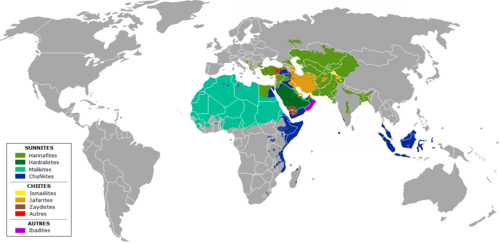
\includegraphics{Images/image097.png}
\vide{ruxe9ponse-soufie}{%
\subsection{Réponse soufie}\label{ruxe9ponse-soufie}}

Je vous propose de lire la lettre du Cheikh Ahmad al-Alawī
(1874-1934)~intitulée «~Lettre ouverte à celui qui critique le
soufisme~».

\vide{v--les-ordres-confruxe9riques}{%
\section{Les ordres
confrériques}\label{v--les-ordres-confruxe9riques}}

Il y en a une cinquantaine dans le monde.

\begin{itemize}
\item
  \textit{La qādirīya} \label{Def:Soufiqādirīya}
Fondateur~: `Abd al-Qādir al-Ğīlānī (m. 1166)
Implantation~: dans tous les pays musulmans, du Maghreb à la Chine


\item
  \textit{La Naqchabandīya} \label{Def:SoufiNaqchabandiya}
Fondée au milieu du XIV° siècle
Implantation~: du Caucasse au Turkestan et à l'Inde
Elle a nourri le nationalisme kurde


\item
  \textit{La Šāḏilīya} \label{Def:Soufisadiliya}
Eric Geoffroy dit de la \emph{Šāḏiliyya} qu'elle est l'une des
«~voies-mères~» du soufisme. Elle est apparue entre la fin du
XII\textsuperscript{e} siècle et le XIV\textsuperscript{e} siècle.
D'origine maghrébine, elle s'est diffusée au XIII\textsuperscript{e}
siècle, à partir de l'Égypte, dans la majeure partie du monde musulman.
Son enseignement est dense et il s'appuie sur les écrits d'Ibn
\emph{`}Arabī.
\end{itemize}
Toute voie initiatique a pour but de mener ses adeptes vers la sainteté,
ou «~proximité divine~» (\emph{walâya})~; celle-ci est identifiée au
plus haut degré de la gnose par al-Shâdhilî. De façon schématique, les
premiers maîtres shâdhilis distinguent deux niveaux~: la sainteté
«~mineure~» (\emph{sughrâ}), ouverte au public large des fidèles, et la
sainteté «~majeure~» (\emph{kubrâ}), réservée à une élite spirituelle.
Mais le terme \emph{walâya}, tout comme celui de sainteté en français,
est un terme générique, un idéal qui implique une méthode pour y
parvenir.

Pour les Shâdhilis, la réponse est claire~: c'est dans l'imitation
intérieure du Prophète que se réalise la \emph{walâya}. Réapparaît ici
le débat millénaire sur les rapports entre \emph{walâya}et
\emph{nubuwwa}, la prophétie, débats qui ont partagé exotéristes et
ésotéristes de l'islam, mais aussi les milieux soufis. Autant les
maîtres shâdhilis initiaux se réclament du premier théoricien de la
sainteté en islam, al-Hakîm al-Tirmidhî (m. 318/930), autant ils s'en
éloignent lorsque celui-ci accorde à la \emph{walâya}une autonomie par
rapport à la \emph{nubuwwa}~: pour eux, la première est subordonnée à la
seconde, et puise sa substance même dans la Lumière muhammadienne
(\emph{al-nûr al-muhammadî}).

\begin{itemize}
\item
  \textit{La Bekt'āchīya}
Elle impose le célibat
De nombreux affiliés en Turquie et Albanie


\item
  \textit{La Tidjānīya}
Influente au Maghreb et dans l'Afrique occidentale


\item
  \textit{La Chattārīya}
Influente en Inde et Malaisie

\item
  \textit{La Rah'mānīya}
La plus influente confrérie algérienne.


\item
  \textit{La mawlāwīya} (derviches)
\end{itemize}

Il existe plusieurs ordres soufis, mais l'on peut distinguer deux grands
groupes de mystiques~: ceux qui se trouvent dans la station de l'ivresse
(\emph{sukr}) et ceux qui sont dans la station de la sobriété
(\emph{sahw}).

Les initiés ivres sont souvent les disciples d'Abū Yazīd Bistamī (m.
875)~: l'ivresse, c'est la perte de sens commun, de la maîtrise de soi.
L'âme est enivrée de la connaissance de Dieu, plongée dans la
contemplation de Dieu.

Pour le second groupe, l'ivresse n'est qu'un état transitoire. Elle est
le début de l'unicité, mais elle se caractérise par la sobriété, quand
il sait que le soi n'est qu'un miroir dans lequel se réfléchit l'Essence
divine.

\paragraph{Pour aller plus loin}

Martin \textsc{Lings}, \emph{Qu'est-ce que le soufisme~?} traduit de
l'anglais par Roger du Pasquier, Paris, Éditions du Seuil, 1977.

Eric \textsc{Geoffroy},
«~\url{http://www.facebook.com/topic.php?uid=21148739744\&topic=3226}{L'islamité
du soufisme et son apport à la spiritualité universelle}~» dans
\url{http://www.religioperennis.org/documents/geoffroy/islamitesoufisme.pdf}

Eric \textsc{Geoffroy}, \emph{Initiation au soufisme}, Coll. L'espace
intérieur, Paris, Fayard, 2003.

Alberto Fabio \textsc{Ambrosio}, \emph{Vie d'un derviche tourneur}.
Doctrine et rituels du soufisme au XVII\textsuperscript{e} siècle,
Paris, CNRS Edition, 2010, 1 vol., 406 pages.

Laleh \textsc{Bakhtiar}, \emph{Le soufisme}. Expressions de la quête
mystique, Paris, Seuil, 1977.

Christian \textsc{Bonaud}, \emph{Le soufisme al-taṣawwuf et la
spiritualité islamique}, Préface de

Michel Chodkiewicz, Maison Larose, IMA, 1991.

\textbf{Exercice pour la Validation}

À partir de la lettre du šaḫy Ahmad al-Alawī, identifierez les éléments
qui répondent aux critiques adressées aux soufis et à Ibn `Arabī tels
que nous les avons exposés.



\chapter{Les racines de la réforme : le
renouveau islamique des XVIIe-XVIIIe
siècles}
\mn{(24/01/2022)}

Un leçon sur les racines de cette diversité, et de tous ces courants au sein du monde Sunnisme. Tout cela part du désir de "\textit{Réforme}" qui part à un retour au source. Et cela peut donner des solutions très diverses, soit des lectures libérales ou des lectures fondamentalistes (un peu comme les évangéliques protestants).
Plutôt \textit{Renouveau} que \textit{Réforme}.

%------------------------------------------------
\section{La crise interne du monde musulman}
\subsection{Déclin des grands empires}

 
 \begin{Synthesis}[Date Symbolique]
 1798 : Napoléon en Egypte, date symbolique de la rencontre du monde musulman avec la modernité occidentale.
 \end{Synthesis}
 Cette lecture n'est pas fausse et va donner lieu au \textit{réformisme} mais c'est une lecture occidentalo-centrée.
 En réalité, cela a commencé plus tôt. Un désir né courant XVII et interne au monde musulman.
 
Les trois grands empires musulmans de l'époque rentrent en crise : 

\begin{table}[h!]
    \sidecaption{Les trois grands Empires musulmans}


%\newlength\q
\setlength\q{\dimexpr .25\textwidth -2\tabcolsep}
\footnotesize%
\noindent\begin{tabular}{p{\q}p{\q}p{\q}p{\q}}
\toprule
                & Fondation           & Apogée                            & Fin                                                                                \\
\midrule
Empire Safavide & 1501 (Ismaïl   1er) & Abbas Ier (1588-1629)             & 1736                                                                               \\
Empire Moghol   & 1526 (Babur)        & Akbar (1556-1605)                 &  1857 (existence symbolique après 1761)  \\
Empire Ottoman  & 1299 (Osman 1er)    & Soliman le Magnifique (1520-1566) & 1922                                        \\
\bottomrule
\end{tabular}


    \label{tab:my_label}
\end{table}
 
 
\begin{figure}[h!]
    \centering
        \sidecaption{Empire Safavide, s'affaiblit
}
 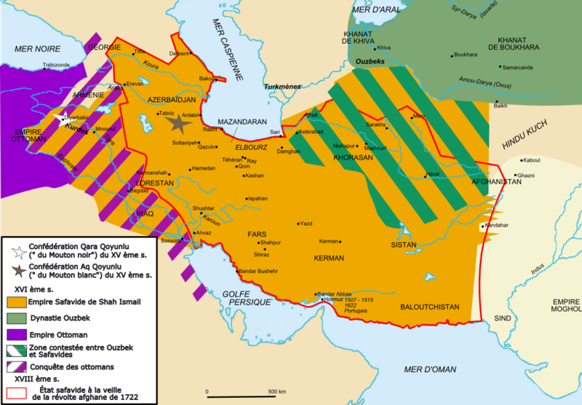
\includegraphics[width=0.9\textwidth]{CourantsIslamContemporain/ImagesCourantsIslamContemporain/empireSafavide.png}

    
\end{figure}


\begin{figure}[h!]
    \centering
        \sidecaption{Apogée et perte de l'empire Moghol : Au XVIII, il est réduit au Rajastan.
}
 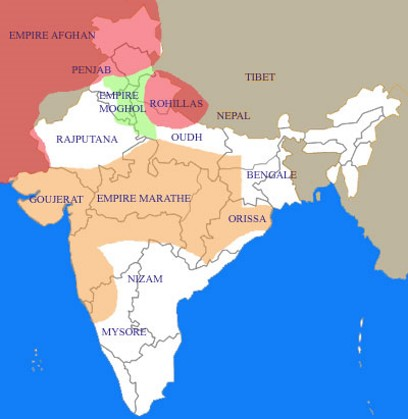
\includegraphics[width=0.44\textwidth]{CourantsIslamContemporain/ImagesCourantsIslamContemporain/Inde18.jpg}
  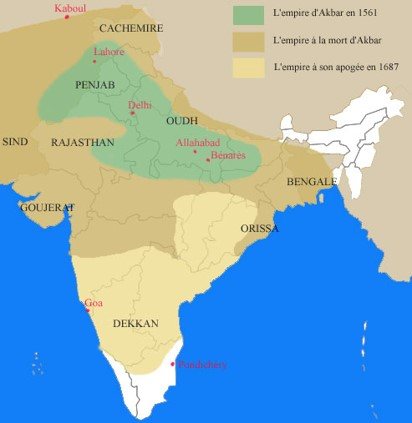
\includegraphics[width=0.44\textwidth]{CourantsIslamContemporain/ImagesCourantsIslamContemporain/empireMoghol.jpg}
\end{figure}

\begin{figure}[h!]
    \centering
        \sidecaption{Déclin Empire Ottoman
}
 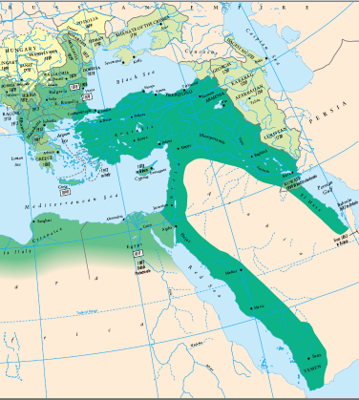
\includegraphics[width=0.5\textwidth]{CourantsIslamContemporain/ImagesCourantsIslamContemporain/declinEmpireOttoman.png}
\end{figure}
 
 \paragraph{Raisons économiques} Les portugais contournent l'Afrique et contournent les empires musulmans.  
 \paragraph{crises politiques} au sein de ces empires, trop grands. 
 \paragraph{Des voisins puissants} Ces Etats vont perdre des territoires face à des puissances qui ne sont pas musulmanes. L'empire Safavide est attaqué par les Ousbeks. L'Empire Moghol en XVIII siècle s'effondre devant l'empire Marathe (Hindou). L'empire Ottoman resiste mais décline depuis 1686 (siège de Vienne). 
 \begin{itemize}
     \item  {Affaiblissement des sultanats Indonésiens} face aux Hollandais. Java est annexé en 1800. 
  \item {En Chine} les musulmans Chinois (Hui) subissent des pressions des Manchous.
   \item  {Afrique} Les bambaras conquièrent Djenné, Tombouctou et Gao. Les portugais en Océanie. 
  \item {En Asie Centrale}, avancée des Russes (XIVII : Kazakstan et reste de l'Asie Centrale au XIX).
 \end{itemize}

 \paragraph{A la fin du XVI} 1591 : deuxième millénaire de l'Islam; sentiment millénariste. \mn{Calendrier lunaire, donc décalage}
 
 
 
\subsection{Problèmes doctrinaux et religieux}

\paragraph{Un raidissement des écoles juridiques au XVII}
Elles s'accusent les unes les autres de ne pas être juste, sentiment de division du monde sunnite.

\paragraph{Décadence du monde Soufi} On a tendance à considérer les soufis comme à la marge du monde musulman. Pourtant, elles ont joué un rôle social déterminant voire politique. Or, à l'époque, elles sont en crise.
\begin{itemize}
    \item {En faisant des Etats dans l'Etat} 
\item {Laxisme spirituel} Un soufi n'est plus tenu de suivre les prescriptions de l'Islam.
\item {Un rôle de plus en plus important du Sheykh}, le maitre spirituel de la Confrérie, qui transmet la \emph{Baraka}.
\item {Des pratiques spéctaculaire} Le fakirisme. le \emph{Dhikr}, rappel du nom de Dieu et l'on atteint l'Etat de transe, et vont marcher sur des braises. 

\end{itemize}



%------------------------------------------------
\section{L'aspiration au
  renouveau}
\subsection{Millénarisme}


 \begin{Def}[rapport au temps Involutif]
 L'Islam se tourne vers le passé, en Islam, les prophètes viennent toujours rappelés ce qui a été donné à l'origine. et le problème est que les hommes déforment le message transmis. Donc Dieu envoie de nouveaux prophètes pour restaurer le message originel. \textit{le temps corrompt.}
 
 \end{Def}
 vs Evolutif. 
 
 Ce qui fait que Mohammad est le dernier des prophètes, c'est que le message est transmis intact, pour la première fois, donc plus besoin de nouveaux prophètes. Autant, la \textit{pratique} peut se corrompre. 
 Un hadith dit : 
 \begin{quote}
     Slt un dixième de la pratique suffira pour sauver le monde.
 \end{quote}
 
 \begin{Def}[Moujaddid]
 de la racine JDD, nouveau, celui qui renouvelle l'Islam pour le mettre tel qu'il était à l'origine. 
 \end{Def}

 
 \begin{Def}[tajdid]
 Tajdid, le renouveau, qui doit venir régulièrement. Chaque siècle Dieu envoie un \textit{Moujaddid} selon un Hadith du Prophète.
 \end{Def}
 
 
 Il peut y en avoir plus mais à chaque siècle, il y a un grand moujaddid, savant, qui ne fait pas forcément au sein de la communauté. 
  \begin{Ex}
 Ghazali est considéré comme un Moujaddid
 \end{Ex}
 \sn{On retrouve cette tension dans toute religion entre respect de la forme et de fidélité au message d'origine}
 
 \subsection{Quelques grandes figures de la \textit{pre-Reforme}}
 

\paragraph{Ahamad Sirhindi} (Inde, 1564-1624) , essaye de rénover l'Islam et réforme une confrérie, la \emph{Naqshbandiyya} réformée (mujaddidi). 
\paragraph{Muhaddidi} Restaurer le monde musulman et restaurer l'Islam dans sa pureté originelle. Il va opposer 
\begin{itemize}
    \item le \emph{taqlid}, l'imitation (péjorative, servile, non réfléchie) et
    \item l'\emph{ijtihad}, l'effort d'interprétation du Coran et de la Sunna. Retourner aux sources scripturaires pour restrouver le sens authentique de l'Islam
    \item pour éliminer la \emph{bid'a}, très péjoratif, l'innovation
\end{itemize}  

On peut distinguer deux courants : un courant plus libéral et l'un plus fondamentaliste :
\begin{itemize}
    \item le rapport à la Tradition : fondamentaliste ne vont considérer que le Coran et la Sunna, en critiquant les élaborations savantes de l'Islam. 
    \item ce sur quoi va porter l'\emph{ijtihad}, soit limité sur les versets peu clairs du Coran, soit plus large pour le savant et les différentes sciences qui vont être convoquées pour l'ijtihad.
\end{itemize}


\paragraph{Muhammad 'Abd Al-Wahhab } 'Arabie, 1703-1792). Voir p. \pageref{Theol:AlWahhab}

\paragraph{Shah Wali Allah} (Inde, 1703-1762), \label{Theo:waliAllah} a eu les mêmes professeurs que Al-Wahhab ! et l'un des premiers à traduire le Coran dans une langue vernaculaire (en persan). Effort d'acculturation dans le contexte Moghol et Indou. 




 
%------------------------------------------------
\section{Les voies du renouveau} 
\subsection{Les confréries soufies}

La création de néo-confrérie
\begin{itemize}
    \item lutter contre un laxisme moral
    \item lutter contre le pouvoir du Sheykh.
    \item insister sur le côté social, en prenant en charge la société (vs gnosticime ?).
\end{itemize}
\mn{Soufi : \pageref{Def:SoufiNaqchabandiya}, \pageref{Def:Soufiqādirīya} }




\paragraph{Ahmad Al Tijani} (Algérie 1737, 1815). Et fonde la \emph{\textbf{tijaniyya}}, un groupe toujours très présent en Afrique du Nord. Normalement un Sheykh insiste sur la chaine d'initiation qui remonte au prophète. Lui, va être initié directement en rêve par le Prophète.

\paragraph{Abdurrauf al-Singkili} (Aceh, Indonésie, 1615-1693)

\paragraph{Abdelkarim al-Samman} (Soudan, 1718-1776) => sammaniyya

Au sénégal, aussi une confrérie de type réformée. 
\mn{A completer carte Carte moderne. Il y avait 24 confréries soufis en Arabie avant le Wahhabisme}




%---------------------------------------
\subsection{Les centres de pèlerinage : La Mecque et Médine}

La Mecque et Médine jouent un rôle essentiel, du fait du Hajj. Du fait de l'Empire Ottoman, il y a pacification des parcours du pélerinage, par ailleurs incités par l'Empire.
Et par ailleurs, des centres de formation s'implémentent à la Mecque.  On en profite pour étudier. Se croisent des savants de différentes origines.
Non seulement les centres d'étude mais aussi les confréries, avec leur Sheykh les plus importants s'installant à Médine ou la Mecque. Ils sont initiés à l'enseignement Moujaddidi et vont réformer la confrérie à laquelle ils appartiennent, selon un modèle qui se répète.




%------------------------------------------------
\section{Un aspect particulier : les jihads aux marges du monde   musulman} 


\begin{figure}[h!]
    \centering
        \sidecaption{Le « renouveau » des marges du monde musulman (XVIIIe-XIXe
siècle)  \emph{L'atlas de l'islam depuis 1500}, F. Robinson, Nathan, 1987  
Des petits Etats vont se créer sur des bases confrériques et dont la mission de faire le jihad.
}
 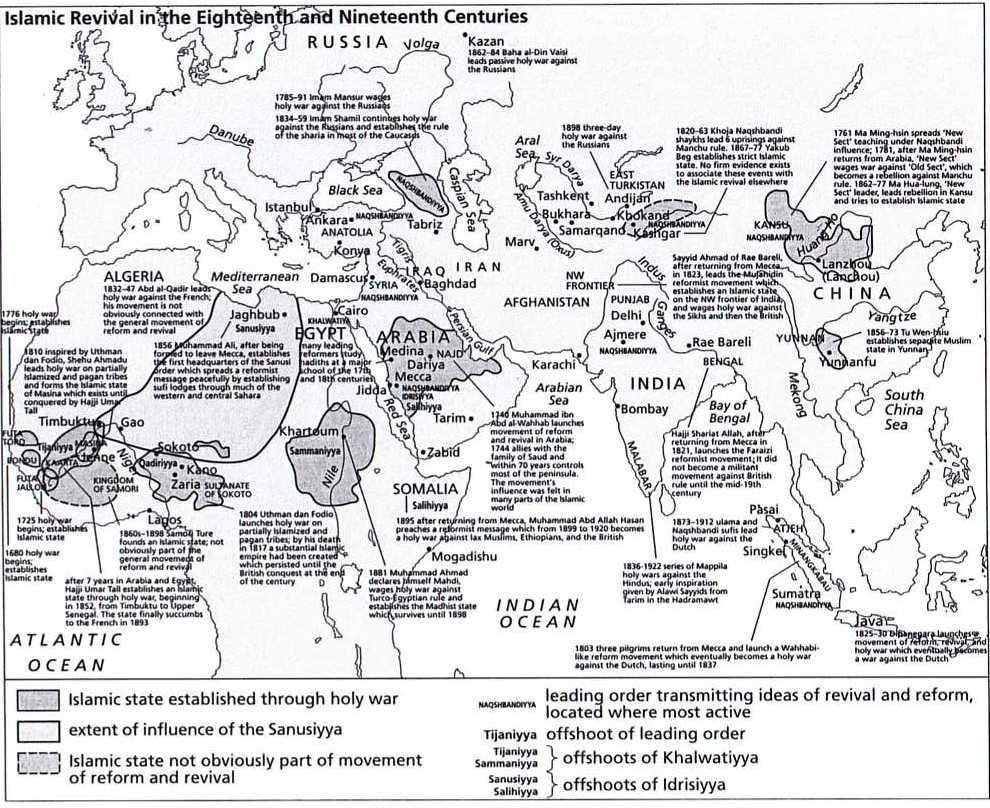
\includegraphics[width=\textwidth]{CourantsIslamContemporain/ImagesCourantsIslamContemporain/image1.jpeg}

    \label{fig:le-renouveau-des-marges-du-monde-musulman-xviiie-xixe-siuxe8cle}
\end{figure}


\subsection{Situation particulière des zones marginales}


Pourquoi on les retrouve aux marges du monde musulman ? Il y a un besoin de purification et l'islamisation par rapport à des populations hétérogènes. Mais aussi, parce que ces zones ne sont pas controlées par les grands empires musulmans qui ne tolèrent pas ces confréries.
Le jihad se porte d'abord sur les musulmans eux-mêmes, pour qu'ils deviennent musulmans puis contre les puissances extérieures ou non musulmanes qui controlent ces zones. 

\paragraph{Une structure Etatique} Le Sheykh est le chef, \emph{Commandeur des Croyants} - on fait référence aux premiers temps musulmans, on prête allégeance, et avec une approche puritaine, très forte pratique. \mn{Des analogiques avec DAESH, qui se réfèrent eux aussi aux temps de l'Islam}

\paragraph{Une accélération de l'Islamisation}


\subsection{Quelques exemples}

\paragraph{Spectre Temporel 1680-1920}{1680, Etat de Bondou} Afrique de l'Ouest jusqu'e l'Etat Mahdiste (Somalie) 1899-1920.

\paragraph{Chine - Ma Ming-hsin} Réveil religieux des communautés chinoises sous la pression des Manchous. Ma Ming-hsin (1719-1781) lorsqu'il est à la Mecque, il fonde une confrérie réformée, la \textit{Nouvelle Secte} et entre en opposition contre les autorités locales, qui appelle en soutien la dynastie Manchoue des Ming. Ming-Hsin est décapité. Il y aura d'autres révoltes plus tard, du Kan-Su et du Chen-Si (1862) et du Yunnan (1856)

\paragraph{Indonésie - Jajji Miskin} Le mouvement Padri à Sumatra (1803-1845). Après le Hajj, en 1803, il prend le contrôle de villages et va imposer sa vision de l'Islam, interdit les pratiques populaires et proclament le Jihad contre les autres villages et les pouvoirs. 1820 : les Hollandais reviennent dans la région et on a une transformation de ce mouvement contre un Jihad contre les Hollandais. Eliminé par les Hollandais.

\paragraph{Nigéria - Califat de Sokoto} Uthman da Fodio (1755-1817) issu d'une famille de savants musulmans, l'enseignement lui vient par la fraderyya\sn{revoir} et crée une communauté qui le reconnait comme \textit{commandeur des Croyants}, s'oppose aux pouvoirs locaux et va être défait par la Grande Bretagne.


\begin{Synthesis}
\begin{itemize}
Ce renouveau : 
    \item Avant la rencontre de l'Occident
    \item lié à des thèmes de crises internes
    \item des thématiques que l'on retrouvera : retourne aux sources scripturaires
    \item C'est assez fascinant de voir la circulation des idées, liée autour du \textit{Hajj}
\end{itemize}


\end{Synthesis}

%------------------------------------------------

 



 



\paragraph{Soufis du Badakhshân : un renouveau confrérique entre
l'Inde et l'Asie centrale}
\mn{Alexandre Papas, \emph{Cahiers d'Asie Centrale}, n° 11-12, 2004, p.
87-102 (extraits -- texte expurgé)}
 
 
\subparagraph{Éléments de biographie d'un soufi
badakhshânais} 
\mn{le Badakhshân est entre l'Afghanistan et le Tajikistan}
\begin{quote}
Mawlânâ Mîr Ghiyâs al-Dîn \label{Theo:MawlanaMirGhiyasAlDin} naît en 1117/1705-06 dans la petite localité
de Hisârak, située au cœur du district de la ville de Jirm. Le
grand-père de Mawlânâ a émigré du village de Dahbîd, non loin de
Samarcande, en direction du Badakhshân. La \emph{silsila}\sn{Génération} de la famille
remonte au Prophète et, sur dix générations, au frère d'un grand saint
Kubrawî et découvre une généalogie \textit{soufie}. C'est donc au sein d'une des
grandes familles \emph{muhâjir}\sn{Emigré, en référence aux premiers musulmans qui ont suivi le Prophète à Médine} de l'aristocratie religieuse du
Badakhshân que naît Ghiyâsî.
\begin{figure}[h!]
    \centering
        \sidecaption{Asie Centrale. On oublie parfois le rôle important de ces états tampon comme lieux d'échange
}
 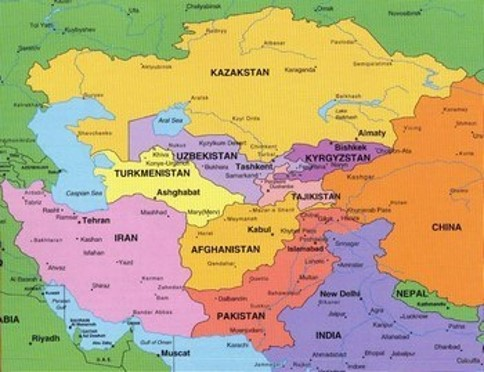
\includegraphics[width=\textwidth]{CourantsIslamContemporain/ImagesCourantsIslamContemporain/AsieCentrale.jpg}
 
\end{figure}

{[}\ldots{]}

C'est précisément pour l'Inde -- destination qui concurrence la
Transoxiane savante, en particulier Boukhara, surtout depuis le XVIe
siècle -- que part le jeune Ghiyâsî âgé de 14 ans en quête d'initiation \sn{soufi}.
Cet exil de l'adolescent fait l'objet de deux contes hagiographiques :
 

\begin{itemize}
\item
 
  Le futur shaykh de Ghiyâsî, Shâh Walî Allâh, qui a quitté Sirhind pour
  entreprendre un pèlerinage au mausolée de Bahâ' al-Dîn Naqshband\sn{le fondateur de la confrérie réformée Naqshandayyi} non
  loin de Boukhara, stationne au Badakhshân, à Jirm, chez le père même
  de Ghiyâsî. Le shaykh demande alors à ce dernier de lui amener ses
  enfants, mais perçoit par claire-vue qu'on lui dissimule le jeune
  Mawlânâ qui, en état de \emph{majzûb}\sn{Ils peuvent faire des choses indécentes} « ravi en Dieu », suscite la honte de
  sa famille. À sa vue le shaykh indien cite un vers de Ni'mat Allâh
  Walî Kirmânî. Et au jeune Ghiyâsî de prononcer miraculeusement le
  second vers du distique. Walî Allâh annonce alors qu'à son retour de
  Boukhara il prendra le jeune homme comme disciple et l'emmènera en
  Inde.
  
\item
 
  Dès l'âge de 9 ans Mawlânâ refuse les conseils de sa famille et se
  distingue des autres enfants. Plusieurs nuits, au cours de rêves, lui
  apparaît un homme illuminé qui lui enjoint de partir pour l'Inde où
  lui est promise la rencontre d'un grand saint soufi. Malgré le refus
  de ses parents qui souhaitent marier leur fils, Ghiyâsî parvient à
  quitter le Badakhshân quelques années plus tard. Parvenu à Lahore et
  après un nouveau rêve révélateur, il attend de nombreux jours au
  couvent de Khwâja Khwândamîr, un khalîfa de la Naqshbandiyya, jusqu'au
  jour où il rencontre Shâh Walî Allâh.
 
\end{itemize}

 
Restent les faits : après une formation classique en \emph{madrasa} à
Delhi où le novice rencontre ses premiers maîtres, il devient à Lahore
durant douze années le disciple d'un fameux maître Naqshbandî Mujaddidî.
Il interrompt une unique fois son initiation lorsque le shaykh lui
confie la mission de se rendre au Cachemire afin d'aller chercher un
homme qu'on prétend thaumaturge et que Walî Allâh souhaite convertir à
l'islam et initier à sa \emph{tarîqat}\sn{confrérie}. Au terme de ses douze années de
noviciat, le shaykh lui enjoint de retourner à sa terre natale pour
propager la confrérie. De retour au Badakhshân, Ghiyâsî âgé de trente
ans environ et qui a obtenu le rang de \emph{mawlawiyyat}\sn{maître}, fait office
d'enseignant à la \emph{madrasa} Jâmi'-i Islâmî du district de Jirm. Il
est ensuite convié à Fayz Âbâd à la cour de Sultân Shâh, laquelle abrite
des savants et des poètes venus d'Inde et d'Iran, dont certains
acquièrent grande réputation. C'est là que Ghiyâsî compose son œuvre
poétique et mystique. C'est également là, de son \emph{khânaqâh}\sn{couvent soufi, Ḵānqāh ou ḵānāqāh, fut d'abord un lieu destiné à abriter les spécialistes et savants religieux musulmans (‘ulamâ’), une sorte d'équivalent des couvents chrétiens. Ces établissements ont été ensuite réservés aux soufis.}, qu'il
dirige son enseignement, suivis par de nombreux disciples venus de
toutes les régions alentours. Le soufi badakhshânais devient aussi le
directeur spirituel de Sultân Shâh. Et lorsque ce dernier est capturé à
Qunduz par les ouzbeks du Qataghân en 1179/1765, le vieux maître
conseille durant trois ans le fils et suppléant du shah emprisonné, Mîr
Muhammad Shâh. D'un tel succès et d'une telle influence, Ghiyâsî
apparaît comme l'un des principaux promoteurs de la Mujaddidiyya dans le
Nord de l'Afghanistan.

{[}\ldots{]}
\end{quote}

\begin{Prop}
On retrouve des noms : Walî Allâh (cf p. \pageref{Theo:waliAllah}; l'importance du réseau confrérique; et rôle social (il devient le conseil du sultan).
\end{Prop}

\subparagraph{Savants et soufis au croisement du
Badakhshân}
Le Pamir est un sanctuaire pour les savants hétérodoxes ou bannis (cf Unwân banni d'Egypte du fait de sa lutte sociale).

\begin{quote}
Malgré les obstacles géographiques et en dépit des troubles politiques
qui affectent la fin du XVIII\textsuperscript{e} siècle, le Badakhshân
reçoit la visite de savants religieux qui, pour certains, décident de
s'y installer et interrompent définitivement leur voyage vers l'Inde ou
vers la Transoxiane. Il faut rappeler ici que le Pamir a, de façon
continue dans l'histoire, servi de sanctuaire à des individus frappés
d'ostracisme ou fuyant la répression dans leur région natale. Mais au cours du
XVIII\textsuperscript{e} siècle le sanctuaire se mue en lieu de
renaissance où fleurissent \emph{madrasa}\sn{lieu d'enseignement religieux} et couvent soufis. Le
\emph{Armaghân-i Badakhshân} mentionne le cas de deux étudiants de
Peshawar, Mîr Ahmad Mujaddidî dit `Izhâr' (m. 1259/1843) et son frère
Muhammad Anwar qui, à une date indéterminée durant le règne de Mîr
Muhammad Shâh, se rendent d'abord à Boukhara afin d'obtenir les
compétences du rang de \emph{`âlim}\sn{savant} et qui, lors de leur retour,
s'installent et officient au Badakhshân, pour le premier à Jirm, pour le
second à Bahârak.

Un autre cas de figure est celui, analogue à Ghiyâsî, de ces
badakhshânais qui partent se former aux sciences religieuses, et
éventuellement au soufisme, dans les grands centres de savoir du monde
musulman, proches ou lointains. De ce point de vue, le cas le plus
intéressant -- et malheureusement le plus douloureux faute
d'informations suffisantes et dans l'absence de vestiges de son œuvre --
est celui de Sayyid Abâ al-Hasan « `Unwân ». Né à Jirm en 1123/1711, il
quitte le Badakhshân pour Boukhara afin d'acquérir une formation
théologique. De là `Unwân se rend au pèlerinage de La Mecque et à
Médine, puis il s'installe durant 18 ans en Egypte, probablement au
Caire, où il poursuit son acquisition des sciences islamiques classiques
et commence à enseigner. Mais `Unwân ne se contente pas de dispenser un
enseignement religieux, il prend parti pour les classes populaires
égyptiennes et contre leur oppression par les propriétaires terriens.
C'est du moins la réputation qu'il gagne selon le \emph{Armaghân-i
Badakhshân}, et qui lui vaut d'être banni d'Egypte. `Unwân part alors
pour Istanbul, rejoint Boukhara et reprend son enseignement. `Unwân, qui
prône l'unité de la Communauté des Croyants (\emph{umma}), décide
d'aller prêcher la concorde (\emph{âshtî}) dans le Caucase, peut-être au
moment de l'activisme Naqshbandî de Shaykh Mansûr dans les années 1780.
Mais il renonce à son projet et entre dans une retraite spirituelle
jusqu'à sa mort en 1206/1791, sans être retourné au Badakhshân.
{[}\ldots{]}

\end{quote}

\begin{Prop}
 Dans le deuxième paragraphe, `Unwân se forme à la Mecque et Médine (rôle du pélerinage), rôle social en Egypte et pas seulement religieux. L'importance aussi de l'Unité, l'\textit{Umma}. 
\end{Prop}
 
\subsection{Liste des neo confréries}

\paragraph{Naqshbandiyya}: La Mecque, Damas, Yémen, Inde, Asie Centrale \label{Def:Naqshbandiyya}
                     => Caucase, Chine Occidentale + Orientale, Sumatra.

\paragraph{Qadiriyya}: Proche Orient, Irak, Inde, Asie centrale 
                    => Indonésie (Java, Aceh), Caucase, Afrique

\paragraph{Khalwatiyya}: Egypte => nombreuses branches en Afrique :

\begin{itemize}
    \item \textit{Tijaniya}: Algérie => Afrique de l’Ouest
    \item \textit{Sammaniyya}: Soudan
    \item \textit{Idrisiyya}: Maroc => Sanusiyya (Lybie), Sahiliyya (Somalie),
    \item \textit{Murghaniyya} (Erythrée)
\end{itemize}- 
 
%-----------------------------------------------
\subsection{bibliographie}

\begin{quote}


AZRA, Azyumardi \emph{The Origins of Islamic Reformism in Southeast
Asia}, Asian Studies Association of Australia/KITLV Press, Leiden, 2004.

PAPAS, Alexandre \emph{Soufisme et politique entre Chine, Tibet et
Turkestan}, J. Maisonneuve, Paris, 2005.

*ROBINSON, Francis \emph{Atlas de l'Islam depuis 1500}, Nathan, Paris,
1987 (dispo à la FELS)

*VOLL, John R. « Foundation for renewal and reform », in John L.
Esposito ed., \emph{Oxford History of Islam}, Oxford University Press,
1999, pp. 509-547.
\end{quote}
\chapter{Un fruit du « pré-réformisme » : le wahhabisme}
\mn{ \emph{(31/01/2022)}}

%---------------------------------------------------------
\section{Le wahhabisme}
\paragraph{Pourquoi en parler} C'est un courant qui a presque trois siècles, avec une évolution dans le monde du musulman qui a évolué. Il faut penser l'Islam contemporain dans son contexte.

 
  \subsection{Muhammad Ibn al Wahhab
  (1702-1792)} 
  \label{Theol:AlWahhab}
  
\paragraph{Origine} Son père est \emph{qadi}\sn{juge} et enseignant. Dans le Hadz. Fait un pélerinage à la Mecque. Renouveau

\paragraph{Formation et premières prédications} Proclame le \emph{Tawhid} l'unicité et lutte contre toutes les pratiques "déviantes". Il se heurte aux autorités locales et retourne donc à la Mecque. Il se forme là avec des maîtres d'Arabie et Indien. Puis se rend à Basra, à un autre maître. C'est là qu'il rencontre les si'ites. Il se heurte de nouveau aux autorités locales. Il rentre en Arabie mais \textit{son père y est hostile}. Ce n'est pas un grand savant mais un lettré. 
 
\paragraph{L'alliance avec Ibn Se`ud} Alliance matrimoniale avec un chef de tribu de la Mecque. Il se rend indésirable et il est obligé de partir et il arrive dans le village de Dariya et il y rencontre un autre chef de village, Mohammed Ibn Se'ud, alliance elle aussi politicolo-religieuse et matrimoniale en 1744. Ibn Se'ud accepte la doctrine et al Wahhab légitime l'acquisition de terre par Ibn Se'ud. 

Wahhab enseigne beaucoup  : il écrit beaucoup à des savants (\emph{Oulema}) à l'intérieur et l'extérieur du royaume de Ibn Se'ud. \textit{selon un modèle prophétique}, Mohammad ayant écrit au Basileos,... 

\paragraph{Un développement politique} Conquiert toute l'Arabie Saoudite. En 1818, c'est la fin du premier état wahhabite car l'empire ottoman intervient et execute le fils de Ibn Se'ud.
    
 Il s'appuie sur deux auteurs : 
\begin{itemize}
    \item Ibn Taymiyya (1263-1328), \label{Theol:Taymiyya2} \sn{cf p. \pageref{ibn-taymiyya}}, un vrai penseur
    \item Ibn Qayyim (1292-1350) un de ces disciples
\end{itemize}
 
Ibn Wahhab insiste sur le retour à la source mais en fait il lit le Coran à travers ces deux auteurs.

\paragraph{Une doctrine condamnée} Son père et son frère s'opposent à lui. Une fatwa contre lui du fait de sa critique sur les différentes écoles juridiques et le fait qu'il exclut de la communauté musulmanes ceux qui ne pensent pas comme lui. 

  \subsection{La doctrine wahhabite} 



  \paragraph{Nécessité du retour aux sources} Accentuation des sources, bien sûr le Coran. 
  \begin{itemize}
      \item  \item  Wahhab s'éloigne d'une lecture du Coran ligne à ligne mais propose une analyse \textit{thématique}.
  \item Il rejette aussi le besoin d'une \textit{médiation} humaine pour comprendre le Coran. Il s'oppose aux \emph{Ashraf}, les descendants du prophète \sn{Les Ashrafs ont un statut particulier dans l'Islam} ainsi qu'aux \emph{Imams} dans le si'isme, ainsi que les \emph{sheykhs} soufis.
  \begin{Prop}
  Il n'y a pas besoin de sciences particulières pour accéder au sens du Coran, d'après Wahhab. 
  \end{Prop}
  \item il suis les \emph{Hadiths}, la seule exégèse possible, la \textit{sunna} et rejette les grands commentaires classiques du Coran.  Cela va jusqu'à critiquer la tradition des 4 premiers Califes \textit{bien guidés}. Abu Bakr avait détourné la \textit{zakat} pour ses propres dépenses.
  \item Il reprend la distinction d'Ijtihad, qu'il limite aux versets aux versets obscures, contre le taqlid. Il s'oppose à deux principes de l'Ijtihad : qiyas (recours par analogie : alcool et drogue), \textit{ijama} (consensus des savants : on considère que cela fait autorité \sn{Infaillabilité de la communauté dans les Hadiths}), et le \textit{ra'y}, l'opinion personnelle du juriste. 
  
  \end{itemize}
 
 \begin{Prop}
 Il conteste les principes sous-jacents aux savants qui l'ont précédés. Il y a une tension entre son ambition de revenir au Coran mais en parallèle en se mettant en filiation avec Ibn Taymiyya
 \end{Prop}
 
 
  \paragraph{Une notion centrale : le \emph{tawhid} (unicité divine)}
  
  \mn{{Extraits du \emph{Kitab at-tawid} (Livre de
l'unicité divine) de Muhammad Ibn Wahhab} . {Chapitre 1} : \emph{Tawhid}
Traduction et édition établies en Arabie Saoudite. Allah est traduit par Allah et non Dieu, alors qu'en Arabe, Dieu est traduit par Allah y compris pour les chrétiens arabes. }

\begin{quote}
\emph{Allah-ta`ala} a dit : « Je n'ai créé les djinns et les hommes que
pour qu'ils M'adorent (1 :56)\ldots Et très certainement nous avons
suscité dans chaque communauté un message pour leur dire d'adorer Dieu
et d'écarter le Rebelle (16 :36)\ldots Et voilà que ton Seigneur a
décrété que tu dois n'adorer que Lui et faire preuve de bonté envers tes
parents (17 :23)\ldots Adorez Dieu et ne lui donnez quelque associé que
ce soit (4 :36)\ldots Venez, je vais vous réciter ce que votre Seigneur
vous a interdit ; - ceci : Ne lui associez quoi que ce soit\ldots(6
:151-153) ». Ibn Mas`ud a dit : « Quiconque se propose de vérifier le
testament du Prophète Muhammad (SWA) -- un testament sur lequel le
Prophète a apposé son sceau, qu'il lise ces mots d'Allah : « Venez, je
vais vous réciter ce que votre Seigneur vous a interdit ; - ceci : Ne
lui associez quoi que ce soit\ldots Voilà ce qu'il enjoint » (6 :
151-153)


Mu`adh Ibn Jabal raconta : « Je montai derrière le Prophète (SAW) quand
il me dit : « Ô Mu`adh ! Sais-tu ce que les créatures d'Allah Lui
doivent et ce qui leur est dû ? » Je répondis : « Allah et son Prophète
savent mieux ». Il continua : « Ce que les créatures d'Allah Lui
doivent, c'est de ne jamais associer qui que ce soit avec Lui. Ce qui
leur est dû, c'est qu'il ne punira aucune personne qui ne Lui associe
pas un autre ». Je dis :

« Ô Prophète d'Allah, est-ce que je peux annoncer la bonne nouvelle aux
gens ? » Il répliqua : «Non ! Ne leur dis rien de peur qu'ils comptent
sur la promesse et manquent à leurs devoirs envers Lui». Ce hadith est
mentionné dans deux \emph{Sahihs}.


D'autres points :


\begin{enumerate}

\item
  \begin{quote}
  La sagesse dans la création du djinn et de l'humanité.
  \end{quote}
\item
  \begin{quote}
  Le service à Allah consiste en le \emph{tawhid}. Car, à l'opposé du
  \emph{tawhid} se trouve l'aliénation d'Allah. (\ldots)
  \end{quote}
\item
  \begin{quote}
  La sagesse d'envoyer des prophètes. (\ldots)
  \end{quote}
\end{enumerate}
  \end{quote}
  
On trouve une accumulation de versets coraniques sur le thème, puis des hadiths du prophète. Le grand péché par excellence, c'est le \emph{shirk}, l'associationisme des Dieux à Dieu. Or Wahhab va plus loin. 

\begin{quote}


\emph{Allah-ta`ala} dit : « Ceux qui ont cru et n'ont point revêtu de
prévarication leur foi\ldots{} » (6 : 82).

(\ldots) Abu Sa`id al Khudriyy rapporta que le Prophète d'Allah (SWA) a
dit : « Quand Musa {[}Moïse{]} demanda à Allah de lui enseigner une
prière qu'il puisse réciter à chaque fois qu'il pensait à Lui ou qu'il
L'évoquait, Allah répondit : « Dis, ô Musa, qu'il n'y a d'autre Dieu
qu'Allah. Musa dit : « Ô Seigneur, tous tes serviteurs prononcent ces
mots ». Allah dit : « Ô Musa, si les sept cieux et tout ce qu'ils
renferment, et les sept terres aussi, si tout cela était pesé contre
cette phrase : « Il n'y a d'autre Dieu qu'Allah », cette dernière
pèserait plus lourd ». Ibn Hibban rapporta cela également et al-Hakim
compléta sa version. Al-Tirmidhi enregistra, avec peu de rédaction, le
récit de Anas à l'effet qu'il entendit le Prophète d'Allah (SWA) dire :
« Allah dit : « Ô Homme ! Si tu venais à Moi avec tous les sacs du monde
remplis de tes péchés, mais avec le témoignage que tu n'associes rien à
Moi, Je viendrais à toi avec tous mes sacs remplis de miséricorde et de
pardon ! ».

    
\end{quote}

\begin{Synthesis}
Si on respecte le \emph{Tawhid}, cela suffit à pardonner les péchés, mais important de respecter les principes de l'Islam (c'est pour cela que c'est caché)
\end{Synthesis}

\paragraph{Distinction au sein du Tawhid } 
\begin{Def}[Le grand Shirk ]
Il distingue le \emph{tawhid rububiyya} (l'unicité de souverainté du monde) avec le \emph{tawhid uluhiyya} (de divinité) : ne reconnaitre aucun intermédiaire entre Dieu et les hommes. Il ne peut y avoir de dévotion que pour Dieu seul : les saints, les soufis, les Imams.
\end{Def} 
Al Wahhab introduit une critique fondamentale contre le soufisme. 

\paragraph{Le petit Shirk} 
\mn{{Chapitre 4} : La crainte du \emph{shirk}}
\begin{quote}
Allah -- qu'Il soit loué et glorifié -- dit : « Non, Dieu ne pardonne
pas qu'on Lui donne quelque associé. En deçà, Il pardonne à qui il veut
» (4 : 48, 116)

(\ldots) Dans le hadith, nous lisons : « Ce que je crains le plus pour
vous, c'est le moindre \emph{shirk}. Quand on lui demanda ce que
c'était, le Prophète répondit : « l'hypocrisie ». Dans le Sahih
d'al-Bukhari, nous lisons que Ibn Mas`ud reporta : « Le Prophète d'Allah
(SWA) a dit : « Celui qui rencontre Allah le jour du Jugement sans Lui
avoir associé qui que ce soit ira au Paradis, et celui qui le rencontre
ayant fait le contraire sera consigné en Enfer ».
\end{quote}
\begin{Def}[le Petit Shirk]
Toute attitude de l'homme qui ne sert pas Dieu. il relève aussi de l'attitude morale.
\end{Def}

\begin{Ex}[L'appel à témoigner qu'il n'y a d'autre
Dieu qu'Allah]

\mn{{Chapitre 5} : }
\begin{quote}
\emph{Allah-ta`ala} a dit : « Dis (ô Muhammad) : `\,`Voici mon sentier,
j'appelle à Dieu'\,' » (12 :108)

Ibn `Abbas (RA) rapporta : « Quand le Prophète d'Allah (SAW) envoya
Mu'adh à al-Yaman, il lui recommanda : `\,`Quand tu rencontres des gens
du Livre, que ta première action soit de leur demander de témoigner
qu'il n'y a d'autre Dieu qu'Allah'\,' ». Selon un autre récit, «
\ldots{} de leur demander de réaliser l'unicité d'Allah. S'ils
t'obéissent, informe-les qu'Allah leur a imposé la \emph{salat} cinq
fois par jour. S'ils t'obéissent en cela, alors informe-les qu'Allah
leur a imposé le devoir de charité qui doit être perçue des riches pour
être distribué aux pauvres. S'ils t'obéissent en cela, ne touche pas à
leurs autres biens et occupe-toi de la plainte de l'opprimé, car il n'y a aucun obstacle dans son accès à Allah ».
(Rapporté dans les \emph{Sahihs} d'al-Bukhari et de Muslim). (\ldots)
\end{quote}
\end{Ex}



\paragraph{Les Intercessions} L'intercession est limitée à Mohammed, et uniquement aux musulmans suivants Wahhab. On ne peut pas prier le Prophète. Peut être intervient-t-il au jugement dernier.


\mn{{Chapitre 17} : L'intercession}
\begin{quote}
Allah -- qu'il soit loué et glorifié -- a dit : « Et par ceci (le
Qur'an), avertis ceux qui, n'ayant pour eux hors de Dieu, ni ami ni
intercesseur, craignent d'être rassemblés vers le Seigneur\ldots{} » (6
: 51). Dis : « A Dieu l'intercession tout entière\ldots{} » (39 : 44).
Qui peut intercéder auprès de Lui que par sa permission ?... (2 : 255).
Et combien d'anges dans les cieux ? Leur intercession ne met au large en
rien, sauf après que Dieu l'a permis, en faveur de qui il veut et qu'il
agrée » (53 : 26). (\ldots)

(\ldots) En tant que catégorie générale du Jour du Jugement en laquelle
les mécréants croient, l'intercession est rejetée par le Qur'an. Le
Prophète (SAW) nous informa qu'en ce jour « il sera amené devant Allah.
Il se prosternera lui-même et louera Allah, plutôt que de demander à
intercéder. Alors on lui dira : « Lève-toi ! Parle maintenant et tu
seras entendu ! Demande et il te sera donné ! Intercède et il te sera
accordé ! » (\ldots) L'intercession est donc là pour les croyants
sincères et candides. Elle n'est accordée que par la permission d'Allah
et n'appartient pas aux associationistes. (\ldots)
\end{quote}


\paragraph{Tombe du juste}
Condamnation de celui qui invoque Dieu
auprès de la tombe du juste et, a fortiori, de celui qui invoque ce
dernier.
\begin{Ex}[Un exemple de Grand Shirk]
\mn{{Chapitre 20} : Condamnation de celui qui invoque Dieu
auprès de la tombe du juste et, a fortiori, de celui qui invoque ce
dernier.}
\begin{quote}
Dans le \emph{Sahih}, A'ishah (RAA) rapporta : « Umm Salmah raconta au
Prophète d'Allah (SAW) qu'elle avait vue une église remplie d'images et
de statues en Abyssinie. Le Prophète dit : « Ceux-là sont les pires de
tous les hommes : lorsqu'un membre juste et vertueux de leur groupe
meurt, ils bâtissent une église sur sa tombe et y installent toutes
sortes d'images pour lui. Ils sont coupables de deux méfaits : celui
d'invoquer quelqu'un auprès d'une tombe et celui d'installer des images
». (\ldots)

Ainsi le Prophète interdit cette pratique et condamna celui qui la
suivait. Faire le \emph{salat} sur une tombe est également interdit,
même si aucune mosquée n'a été construite sur l'emplacement. Telle est
la signification de la déclaration suivante : « On craignait qu'elle ne
soit prise pour une mosquée ». Les Compagnons n'étaient pas supposés
construire une mosquée autour de la tombe du Prophète. Tout endroit
destiné au \emph{salat} ou tout endroit où le \emph{salat} est accompli,
est une mosquée. Tel l'a déclaré le Prophète (SAW) : « Toute la terre
est pour moi une mosquée, un endroit pur (pour accomplir le
\emph{salat}) ».
\end{quote}

\end{Ex}


  \paragraph{La question du \emph{jihad}} La question de la violence chez Wahhab. Il faut repartir de la position kharijite. Un calife doit respecter la religion de façon exemplaire. s'il ne le fait pas, il est \emph{Takfir}, mécréant. Or la vision sunnite a jugé que c'est Dieu uniquement qui jugera si un musulman est un non-musulman. Ibn Taymmayyia s'élève contre les souverains Mongols : : les souverains mongols sont certes musulmans puisqu'ils ont adopté la foi musulmane mais en surface.  Wahhab va reprendre ce concept et ceux qui n'adhèrent par au \emph{shirk} sont apostats. Un germe de violence.
  
  \begin{Synthesis}
  On voit donc l'extension du concept de Ibn Taymmayyia sur le Takfir à tout le shirk, et donc en pratique en non respect du wahhabisme.
  \end{Synthesis}
 
 Mais il n'y a pas de volonté de jihad dans le wahhabisme. On peut même faire des traités avec des non-musulmans.
 
  \section{Le devenir du wahhabisme} 
 
  
 

% ------------------------------ 
\subsection{Les trois Etats Saoudiens} 

 
  {\paragraph{1744 -1818}: une première expansion}
 
 
\emph{1744} alliance Ibn Se`ud /Ibn al-Wahhab
 
\emph{1786} conquête du Najd (`Abd-al-`Aziz)
 
\emph{1792} mort d'Ibn al-Wahhab
 
\emph{1806} conquête de La Mecque
 
\emph{1818} défaite devant les Ottomans
 

 
  {\paragraph{1821-1883}: petit Etat centré sur Riyad (Najd)}
 
  {\paragraph{1901- 2011} : le Royaume d'Arabie Saoudite} Un descendant de Wahhab qui repasse alliance avec la famille de Se'ud et conquiert l'Arabie. 
 
 
\emph{1924} conquête de La Mecque. Abdelaziz Ibn Se`ud prend le titre de
roi et \textit{protecteur des lieux saints}. On détruit les confrérie, on contrôle le pélerinage, on supprime les autres écoles de droit.

\mn{REVOIR}

\emph{1939} début de la production pétrolière \emph{1962} création de la
Ligue islamique \emph{1990} début de la guerre du Golfe.
 

 
\subsection{L'Arabie Saoudite et l'économie
pétrolière} 
 
\paragraph{ {Début de la
production}} 

\begin{quote}
1935: premier forage

1939: premier baril de pétrole

⇒ Cartel américain: l'ARAMCO
\end{quote}

 
\paragraph{{Nationalisation de la
production}}


1973: l'Etat s'approprie 25 \% des droits de l'ARAMCO (1974 : 60\%, 1980 : 100\%)


⇒ Saoudi ARAMCO: 95 \% de la production du pays.

 
\paragraph{Evolution du cours du
pétrole} 

\begin{quote}
1973: premier choc pétrolier (guerre de Kippour) =\textgreater{} de 4 à
15 \$/B

1981-1983: deuxième choc pétrolier (Révolution iranienne + guerre
Iran-Irak) =\textgreater{} 36 \$/B 2006-2008: troisième choc pétrolier
(guerre en Irak) =\textgreater142 \$/baril
\end{quote}

\paragraph{{Rente}}: 1973-2002 =\textgreater{} 200 000 milliards
de dollars au total
 
    Une étude de cas : le wahhabisme en Afrique de l'Ouest
    
\subsection{Le wahhabisme et l'Etat saoudien}

Le wahhabisme accepte une certaine ouverture en Arabie en contrepartie de financement extérieur. On est dans des \textit{concessions} des oulemas. 

\paragraph{La ligue islamique 1962} on étudie gratuitement à la Mecque et à Médine pour propager le wahhabisme.

 
\subsection{Une étude de cas : le wahhabisme en Afrique de l’Ouest}

\paragraph{Des étudiants revenant de la Mecque dans les années 40} et surtout depuis dans les années 70, avec la ligue islamique. 

\paragraph{Un conflit avec les structures soufis}, maraboutisme, très puissantes. On ne priait pas dans les mêmes lieux de culte. 1978 : On  est  loin de  l'époque  où,  en  1978,  Yao  Koum  expliquait  au  Ministre  de  l'Intérieur  qu' \sn{Le wahhabisme à Abidjan Marie Miran-Guyon \url{https://halshs.archives-ouvertes.fr/halshs-01062687/document}}
\begin{quote}
    "obliger  un musulman  orthodoxe (wahhabite)  à  prier  derrière  un  musulman  traditionnel,  c'est  le  contraindre  à renoncer  purement  et  simplement  à  sa  religion,  c'est  l'anéantir  moralement".
\end{quote}


 % -------------------------
\subsection{ {Glossaire}} 


\paragraph{Personnes} `Abd al --`Aziz Abu Bakr

al-Majmu`i al-Sindi

Ibn Taymiyya Muhammad Ibn Se`ud

\paragraph{Lieux}

al-Azhar al-Dir'iyah

al-Uyaynah (Najd). Basra

Hijaz Huraymila Jeddah Najd

\paragraph{Notions}

ashraf : \emph{descendants du Prophète}

da`wa \emph{: prédication}

fiqh : \emph{droit musulman}

hadith \emph{: fait ou dire du Prophète}

hijra : \emph{« exode »}

ijma\emph{` : consensus des ulamas}

ijtihad : \emph{effort d'interprétation}

kufr \emph{: incroyance /} 

kafir \emph{: infidèle, mécréant}

qiyas \emph{: raisonnement par analogie}

salat : \emph{prière rituelle} 

shirk : \emph{associationnisme} 

taqlid
\emph{: imitation (servile)} 

tawhid : \emph{unicité divine}

zakat :
\emph{aumône légale}

 %-----------------------------------------------------
\subsection{Extraits du \emph{Kitab at-tawid} (Livre de
l'unicité divine) de Muhammad Ibn Wahhab}
\mn{Traduction et édition établies en Arabie Saoudite}

\paragraph{{Chapitre 2} : Les vertus du \emph{tawhid} et les
nombreux péchés qu'il expie}



\paragraph{{Chapitre 27} : Les motivations mondaines sont des
exemples de \emph{shirk}}
\begin{quote}
\emph{Allah ta'ala} a dit : « Qui aspire à la vie d'ici-bas et à ses
parures, nous leur solderons ce qu'ils y auront fait : ils ne subiront
pas de perte ! Voilà ceux qui, dans la vie dernière, n'ont pour partage
que le Feu : leurs réalisations d'ici-bas ont crevé ! Nulles sont leurs
œuvres ! (11 : 15-16).

Abu Hurayrah (RAA) rapporta ce hadith \emph{sahih} suivant : « Le
prophète d'Allah (SAW) a dit : `\,`Malheur à l'esclave du dinar !
Malheur à l'esclave du dirham ! Malheur à l'esclave du khamilah !
(\ldots)
\end{quote}
\paragraph{{Chapitre 38} : Obéir aux ulamas ou aux gouvernants
qui légitiment ce qui est interdit ou interdisent ce qui est légitime,
c'est les associer à Allah.}
\begin{quote}
Ibn `Abbas a dit : « Je vous dis que `\,`le Prophète d'Allah (SAW) a dit
ceci et vous dites que `Abu Bakr et `Umar ont dit quelque chose d'autre
?'\,' Le ciel va bientôt vous cracher des pierres sur la tête !! »

Ahmad ibn Hanbal a dit : « Très étranges, en effet, sont ceux qui,
sachant le véritable \emph{isnad} (d'un commandement du Prophète), se
tiennent quand même à l'opinion de Sufyan. Allah lui-même a dit : « Que
ceux donc qui s'opposent à son commandement prennent garde qu'une
tentation ne les atteigne, ou que ne les atteigne un châtiment
douloureux ». (24 : 63). Savez-vous ce que peut être une telle tentation
? C'est le \emph{shirk}. Car, désobéir au Prophète dans certains de ses
commandements, c'est pratiquement comme si on reniait son message et on
s'attirait le Feu.

\end{quote}


\section{bibliographie}

 

\begin{itemize}
\item
 
  IBN AL-WAHHAB, Muhammad \emph{L'unicité de Dieu}, al Qalam, Paris,
  2001.
 


 \item
MENORET, Pascal \emph{L'Énigme saoudienne. Les Saoudiens et le monde
1744-2003}, La Découverte, Paris, 2003.
\item
MIRAN, Marie ; RIALLAND, Maëlle « Dossier Wahhabisme », \emph{Islam et
sociétés au Sud du Sahara}, n°12, 1998, Paris.
\item
MOULINE, Nabil \emph{Les Clercs de l'islam. Autorité religieuse et
pouvoir politique en Arabie Saoudite
(XVIII\textsuperscript{e}-XXI\textsuperscript{e} siècles)}, Paris, PUF,
2011.
\item
  \emph{Histoire de l'Arabie
saoudite}, Paris, Flammarion, 2013.
\item
REDISSI Hamadi \emph{Une histoire du wahhabisme. Comment l'islam
sectaire est devenu l'islam}, Paris, Seuil, 2016.
 \end{itemize}
 
 
\mn{
\href{http://journals.openedition.org/assr}{Archives de sciences
sociales des religions} p. 229-253

\url{https://doi.org/10.4000/assr.21954}}

\section{Les oulémas du palais}

Parcours des membres du Comité des grands oulémas

\hypertarget{ruxe9sumuxe9s}{%
\subsection{\texorpdfstring{\emph{Résumés}}{Résumés}}\label{ruxe9sumuxe9s}}


Véritable matrice idéologique de l'État saoudien et instrument de
légitimation politique et religieuse, la doctrine wahhabite et ses
dépositaires, les oulémas, sont les soutiens indéfectibles de la famille
Sa‛ūd depuis la seconde moitié du e siècle. Cette alliance se renforce,
à partir de 1971, avec la création d'un certain nombre d'institutions
politico-religieuses dont la plus importante est le Comité des grands
oulémas. Si les larges prérogatives, dont dispose cette dernière dans
les domaines politique, religieux et social, poussent l'autorité
politique à vouloir en chapeauter l'action et contrôler l'accès,
l'establishment wahhabite n'en fait pas moins. En effet, l'élite
religieuse saoudienne a adopté des mécanismes d'autorégulation bien
définis pour maintenir son homogénéité et son unité pour mieux dominer
l'espace socioreligieux du royaume. Nous tentons dans cet article, à
partir d'une étude de terrain, de lever le voile sur ces mécanismes en
étudiant les origines sociales et régionales et le cursus honorum des
quarante-cinq oulémas qui siègent ou ont siégé au Comité. Cela permet
d'en ressortir avec le portrait idéal-type de l'ouléma wahhabite
contemporain et de voir dans quelle mesure son parcours le qualifie pour
l'encadrement de la population et du soutien au régime.

\hypertarget{texte-intuxe9gral}{%
\subsection{\texorpdfstring{\emph{Texte
intégral}}{Texte intégral}}\label{texte-intuxe9gral}}

\begin{quote}
\mn{ Paris -- Institut d'Études Politiques,
\href{mailto:mohammednabil.mouline@sciences-po.org}{\nolinkurl{mohammednabil.mouline@sciences-po.org}}}

En s'appuyant sur la doctrine hanbalo-wahhabite, pour légitimer leur
pouvoir et leur hégémonie en Arabie et étendre leur influence dans le
monde musulman, les Āl Sa‛ūd se sont étroitement liés aux oulémas,
dépositaires et interprètes de cet «instrument intellectuel par
excellence de domination politique» en Arabie Saoudite (Al Rasheed,
2007: 28). En échange de la garantie d'autonomie de l'espace religieux
et d'un contrôle plus ou moins étroit de l'espace social, les oulémas
mettent au service de la monarchie saoudienne toutes les ressources
symboliques dont ils disposent pour légitimer ses positions et
sanctifier son action. La consolidation définitive du royaume saoudien,
en 1932, n'a fait que renforcer cette alliance et l'institutionnaliser.

Le flux des revenus pétroliers et la politique de solidarité islamique
menée par la
monarchie saoudienne (Kepel, 2003: 89-92; al-Suwayyigh, 1992: 83-93) a
permis à l'establishment hanbalo-wahhabite de se moderniser en se dotant
de structures administratives et éducationnelles dont la plus importante
est le Comité des grands oulémas. 
\begin{Def}[comité des grands oulémas]
Mise en place en 1971, cette instance,
où siègent en théorie les plus éminents oulémas du pays, et même du
monde musulman, s'est très rapidement imposée comme la principale
instance législative du pays, à côté du conseil des ministres, la
principale instance légitimatrice de l'action politique du pouvoir et le
bouclier idéologique du régime. 
\end{Def}

L'importance que revêt cette
organisation étatique fédérative pour le pouvoir politique saoudien
pousse ce dernier à vouloir en contrôler l'accès et le fonctionnement
pour éviter toute «insubordination» des grands oulémas. De même, l'élite
religieuse veille, à travers ses réseaux formels et informels, à
maintenir sa cohésion et son homogénéité, pour perpétuer l'hégémonie de
son discours, en imposant aux prétendants aux charges «cléricales»
officielles des conditions plus ou moins rigoureuses. Toutefois, aucun
document ne mentionne les conditions que doit remplir un ouléma pour
accéder au Comité. Le seul moyen de lever le voile sur ces conditions
d'accès tacites est de suivre le parcours et le processus de
socialisation des cinquante- deux oulémas qui siègent ou qui ont siégé
au Comité. L'étude des origines sociales,
«ethniques» et régionales des oulémas, de leur formation, de leur
\emph{cursus honorum} et de leur mobilité permettront non seulement de
tirer au clair les conditions d'accès à cette élite mais aussi de jeter
de nouvelles lumières sur les principales caractéristiques de ce groupe
stratifié et différencié. Et pour remettre cette élite dans son milieu
sociopolitique, nous ferons appel, à chaque fois que cela sera possible,
aux autres élites
consultatif1 -- dans le cadre d'un travail de comparaison et de mise en
perspective. Cela permettra, d'une part, d'énumérer les principales
conditions, plus ou moins tacites, d'accès à cette élite et son
évolution, d'autre part, de voir dans quelle mesure l'establishment
hanbalo-wahhabite fait preuve d'auto-encadrement, d'autorégulation, de
reproduction et d'adaptation, sous l'œil bienveillant de l'autorité
politique, pour mieux dominer l'espace religieux saoudien et rayonner
dans l'espace islamique.
\end{quote}

\hypertarget{des-self-made-men-aux-huxe9ritiers}{%
\section{Des self-made-men aux
héritiers:}\label{des-self-made-men-aux-huxe9ritiers}}

\begin{quote}
\textbf{origines sociales des oulémas}

La prédication de Muḥammad b. `Abd al-Wahhāb (m. 1792), qui connaît un
succès fulgurant, fait de nombreux disciples. Du vivant d'Ibn `Abd
al-Wahhāb déjà, plusieurs de ses disciples manifestent zèle et grand
dévouement à la \emph{da‛wa}. À la mort du fondateur du
hanbalo-wahhabisme, il y a routinisation de son charisme, au sens de Max
Weber. Si les membres de sa famille héritent d'une grande partie de ce
charisme, ses disciples eux aussi, bénéficient de la routinisation. Il
en résulte la création d'un certain nombre de «dynasties» d'oulémas
monopolisant l'espace religieux (malgré quelques cas isolés de réussite
individuelle) des trois États saoudiens et ce jusque dans les années
cinquante. Ces «dynasties» d'oulémas sont pour les plus importantes, les
Āl al-Shaykh, descendants directs du cheikh Ibn `Abd al-Wahhāb, les Āl
Sulaym, les Āl `Atīq, les Āl Blīhid, etc. (al-Bassām, 1999; Āl
al-Shaykh, 1973). Mais à partir des années cinquante, une certaine
«démocratisation» de la fonction cléricale voit le jour en Arabie
Saoudite. La liste des membres du Comité des grands oulémas, depuis sa
création en 1971, en est la preuve. Il ressort globalement de nos
entretiens et de la lecture des biographies des membres du Comité
décédés à ce jour, 
\begin{Synthesis}
trois grandes catégories d'oulémas: les self-
made-men, les enfants de ceux qu'on a appelés des «cadres religieux
moyens» et les héritiers des grandes «dynasties» d'oulémas.
\end{Synthesis}

Dans la première catégorie, ont été classés les oulémas d'origine
étrangère et les oulémas saoudiens issus de milieux modestes. Faire des
études et accéder aux hautes fonctions religieuses a offert des
opportunités incalculables à ces oulémas et leur a garanti la promotion
sociale. Mais on remarque que ces ascensions sociales restent tout à
fait exceptionnelles. Dans une société qui fonctionne toujours selon le
modèle segmentaire, la mobilité sociale n'est, en théorie, possible que
si l'individu possède un certain capital culturel et social, capital que
les self-made-men ne possèdent naturellement pas. Cela se fait
d'ailleurs ressentir au sein du Comité car, bien que très respectés pour
leurs qualités personnelles et leur savoir, les self-made-men sont,
malgré cela, «dédaignés» par leurs collègues, à cause de leur origine
sociale. D'ailleurs, la nomination de self-made-men au sein du Comité
des grands oulémas n'est intervenue que trois fois depuis la création du
Comité: une première fois en 1971, la deuxième fois, en 1977 pour
remplacer un membre décédé et la troisième fois, lors du premier
remaniement des membres de la Hay'a, en 1987. Cela peut être expliqué
par le fait que l'Arabie Saoudite souffrait d'un manque de cadres entre
les années cinquante et soixante-dix, ce qui a obligé les autorités à
faire appel à des cadres religieux étrangers en attendant la formation
des cadres «nationaux».

La deuxième catégorie, celle des enfants des «cadres religieux
moyens», est constituée d'oulémas dont les parents, au sens large du
terme, ont exercé des fonctions religieuses telles la magistrature,
l'enseignement, l'imamat d'une mosquée ou encore la prédication, sans
toutefois bénéficier d'une grande renommée. Ils peuvent également
descendre de familles d'oulémas «mineures». Nous avons aussi inclus dans
cette catégorie les oulémas dont les parents ont exercé une profession
libérale, tout en ayant une connaissance du Coran et d'une partie de la
production théologique hanbalo-
wahhabite. Les oulémas issus de cette catégorie constituent plus de 67\%
des membres du Comité des grands oulémas.

Le milieu familial joue un rôle déterminant dans la promotion sociale
de ces oulémas.

Les «cadres religieux moyens» initient eux-mêmes leurs enfants au savoir
religieux ou les confient, le cas échéant, à des précepteurs de
confiance. Le réseau parental ou familial leur permet d'étudier avec les
maîtres les plus réputés et les plus influents et de fréquenter les
bibliothèques les mieux fournies. De plus, l'apprenti \emph{`ālim} de la
génération d'avant le boom pétrolier n'est pas obligé de travailler ou
d'entreprendre, parallèlement, d'autres études pour subvenir à ses
besoins. Il est, en effet, important pour les «cadres religieux moyens»
de former le fils «prodige» pour en faire un grand \emph{`ālim}, dans le
but d'assurer la mobilité sociale pour toute la famille. Car il faut
savoir qu'en devenant grand \emph{`ālim} et membre du Comité des grands
oulémas, il devient, par la même occasion, très aisé financièrement et
très influent.

8 Parmi ces oulémas, ceux qui réussissent à avoir un capital symbolique
restent cependant rares. Plus rares encore, sont les oulémas qui
réussissent à transmettre ce capital à leurs héritiers. Si une telle
transmission se fait, nous assistons à la création d'une «dynastie»
d'oulémas. Cela a été le cas de la famille Ibn Ḥumayd. Issu d'une
famille de «cadres religieux moyens», `Abd Allāh b. Ḥumayd (1911-1982) a
gravi un à un tous les échelons de l'establishment religieux. Grâce à sa
proximité avec Muḥammad b. Ibrāhīm (m. 1969), le grand mufti du royaume
et la principale figure du hanbalo- wahhabisme durant la première moitié
du e siècle, Ibn Ḥumayd a réussi à obtenir le poste de juge dans les
principales villes du Najd dès 1939. Son talent et sa loyauté envers la
dynastie ont poussé le roi `Abd al-‛Azīz à le nommer, en 1953, grand
juge de la province du Hijâz et imâm de la grande mosquée de la Mecque
puis responsable de la gestion des deux lieux saints. Ces postes lui ont
conféré une réputation nationale et Ibn Ḥumayd est peu à peu devenu une
personnalité religieuse incontournable dans le royaume. Il atteint le
sommet de sa carrière dans les années soixante-dix en devenant membre du
Comité des grands oulémas et président du Haut conseil de la
magistrature. Si Ibn Ḥumayd n'est pas le seul exemple de réussite dans
le royaume -- Ibn Bāz (m. 1999) et Ibn `Uthaymīn (m. 2001) sont arrivés
au sommet de l'establishment --, son originalité réside dans le fait
qu'il a réussi à transmettre son capital symbolique à son fils Ṣāliḥ.


\paragraph{9 Ṣāliḥ Ibn Ḥumayd}  Né en 1950, celui-ci poursuit, sous l'œil bienveillant de son père,
une double formation traditionnelle et moderne, sanctionnée par un
doctorat en droit musulman. Il commence alors une carrière universitaire
qui le mène rapidement au sommet de l'establishment. En quelques années,
il devient le doyen de la faculté de théologie de l'Université islamique
de la Mecque. Ses nouvelles fonctions et sa connaissance de la langue
anglaise lui permettent de participer à des rencontres internationales
et de donner une image moderne de l'establishment hanbalo-wahhabite.
Parallèlement, il remplace son père à la tête de l'appareil chargé de
gérer les lieux saints. Il reprend par la même occasion le poste très
prestigieux et médiatique d'imâm dans la grande mosquée de la Mecque. En
1993, Ṣāliḥ b. Ḥumayd est nommé membre du Conseil consultatif. En
décembre 2001, il devient membre du Comité des grands oulémas. Quelques
mois plus tard, il prend la tête du Conseil consultatif. En 2009, il
récupère le poste paternel de président du Haut Conseil de la
magistrature. D'ailleurs, Ibn Ḥumayd prépare déjà ses enfants à prendre
la relève: une «dynastie» est née2.
\end{quote}

\hypertarget{les-ux101l-shaykh-les-luxe9vites-du-hanbalo--wahhabisme}{%
\section{Les Āl Shaykh : les Lévites du hanbalo-
wahhabisme}\label{les-ux101l-shaykh-les-luxe9vites-du-hanbalo--wahhabisme}}

\begin{quote}
10 Toutefois le tableau serait incomplet, si l'on omettait de parler de
la plus grande famille religieuse du pays, qui règne sans partage sur
l'establishment religieux depuis le
e siècle. Il s'agit des Āl al-Shaykh, troisième grande famille du
royaume après les Āl
Sa‛ūd et les Sudayrī et descendants directs de Muḥammad b. `Abd
al-Wahhāb. Ses membres détiennent, en effet, les plus hautes fonctions
religieuses. Le capital symbolique de cette famille s'est transmis, sans
interruption, de génération en génération, depuis l'apparition du
hanbalo-wahhâbisme.

11 Après la mort d'Ibn `Abd al-Wahhāb, ses descendants reçoivent une
grande partie de son héritage spirituel et temporel. Ils allaient
apporter à la famille des Āl Sa‛ūd tout l'appui idéologique dont
celle-ci allait avoir besoin pour étendre son influence et son
territoire. Cette «entente cordiale» profite aux deux parties: les Āl
al-Shaykh confèrent la légitimité aux Āl Sa‛ūd qui, en retour, concèdent
aux Āl al-Shaykh le monopole de l'espace religieux. Une alliance
matrimoniale vient renforcer cette alliance politico- religieuse: le roi
`Abd al-‛Azīz, fondateur du troisième État saoudien, épouse la fille du
premier mufti du royaume `Abd Allāh b. ‛Abd al-Laṭīf. De cette union
naîtra Fayçal, roi d'Arabie Saoudite de 1964 à 1975. Cette alliance
connaît toutefois une grave crise dans les années soixante quand le
grand mufti Muḥammad b. Ibrāhīm entrave les projets
«d'institutionnalisation» de son petit neveu (Ibn Ibrāhīm, 1978: no
4033-4039 et no
4539-4046), le roi Fayçal. À la mort d'Ibn Ibrāhīm, le roi bureaucratise
les oulémas: les Āl al-Shaykh sont évincés des principaux postes
religieux3. De 1971 à 1987, seul un membre de la famille Āl al-Shaykh,
Ibrāhīm b. Muḥammad b. Ibrāhīm, destiné initialement à succéder à son
père au poste de grand mufti, exerce une haute fonction étatique. Il est
membre du Comité des grands oulémas et ministre de la justice.
L'humiliation a été grande suite à la nomination, à la tête de
l'establishment hanbalo- wahhabite, de `Abd al-`Azīz b. Bāz, un
\emph{ḫaḍīrī} ou citadin d'origine non tribale, issu d'une famille de
«cadres religieux moyens».

12 Ce n'est qu'à partir de la seconde moitié des années
quatre-vingt-dix, que la famille royale décide de revenir
progressivement à l'alliance traditionnelle avec les Āl al- Shaykh. Le
nom de la famille réapparaît alors dans les listes des plus hauts
dignitaires religieux saoudiens. L'année 1999 marque, pour ainsi dire,
le retour à l'état normal des relations entre la famille royale et les
Āl al-Shaykh: `Abd al-`Azīz b. `Abd Allāh Āl al- Shaykh est nommé grand
mufti du royaume et président du Comité des grands oulémas. Depuis, les
membres de la «dynastie» d'oulémas des Āl al-Shaykh réinvestissent, peu
à peu, la majeure partie des fonctions qu'ils occupaient autrefois.
Outre le grand mufti, deux membres de la famille siègent au Comité des
grands oulémas, un membre de la famille Āl al-Shaykh est ministre des
affaires islamiques, un autre est ministre de la justice puis président
du Conseil consultatif.

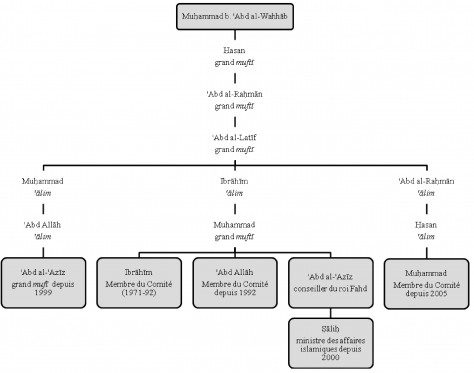
\includegraphics[width=\textwidth]{CourantsIslamContemporain/ImagesCourantsIslamContemporain/genealogie.jpeg}

13 Reste à signaler le cas particulier des oulémas originaires du Hijâz
et d'al-Aḥsā', provinces connues pour leur organisation hétéroclite. En
effet, la plupart des membres du Comité des grands oulémas, originaires
de ces régions, sont issus de ce qu'on a appelé des «dynasties»
d'oulémas, \emph{buyūtāt `ilm}, ou maisons de savoir comme ils aiment
eux-mêmes se faire appeler (à l'instar des familles d'oulémas dans les
autres pays arabes). Plus important encore est le fait que les familles
de ces oulémas appartiennent aux quatre écoles juridiques du sunnisme.
Si le facteur familial revêt une importance certaine, le paramètre de
l'origine tribale doit aussi être pris en compte.
\end{quote}

\hypertarget{la-pruxe9dominance-du-croissant-najdux12b}{%
\section{\texorpdfstring{La prédominance du croissant
\emph{najdī}}{La prédominance du croissant najdī}}\label{la-pruxe9dominance-du-croissant-najdux12b}}

\begin{quote}
14 Force est de constater que l'appartenance à une tribu, généralement
réinventée, constitue un critère identitaire important, dans une société
qui commence à peine à s'individualiser: avant d'être citoyen ou sujet,
on appartient d'abord à une tribu. C'est dire l'importance du milieu
tribal en tant que champ de socialisation des individus. La
\emph{`aṣabiyya}, l'esprit de corps tribal, joue un rôle fondamental
dans le statut social et la promotion de l'individu en Arabie Saoudite.

15 Les oulémas d'origine tribale dominent largement le Comité des grands
oulémas (il s'agit des tribus sédentarisées à partir du e siècle). Ils
sont quarante et un sur les cinquante-deux membres qu'a comptés le
Comité, depuis sa création, à être d'origine tribale, soit 79\%. Les
oulémas d'origine tribale se taillent ainsi la part du lion depuis 1971.
Les onze sièges restants sont occupés par des oulémas issus de trois
milieux différents: des membres de la notabilité citadine du Hijâz
(cooptés pour représenter les intérêts de leur région: on essaie de
choisir les plus «wahhabisés» et/ou quiétistes des oulémas du Hijâz),
des étrangers naturalisés (ils sont hanbalo-wahhabites, ont des talents
«exceptionnels» et ont défendu le hanbalo-wahhabisme et l'État) et des
citadins du Najd, sans affiliation tribale ou \emph{ḫaḍīrī}-s (ces
derniers ne doivent, en principe, leur ascension sociale qu'à leurs
compétences personnelles).

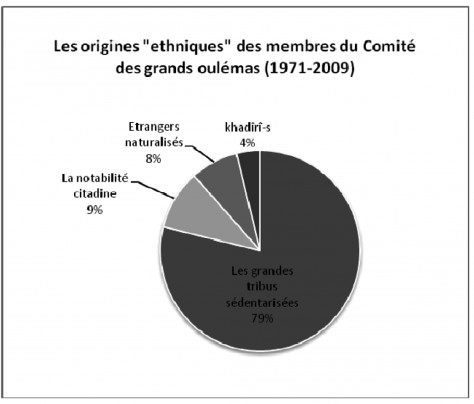
\includegraphics[width=4.9375in,height=4.20833in]{Image/media/image10.jpeg}

16 On constate alors, chiffres à l'appui, que l'appartenance au milieu
tribal sédentarisé joue un rôle déterminant dans l'ascension sociale des
oulémas, la \emph{`aṣabiyya} étant une valeur ajoutée qui permet de se
constituer un capital social. Cela dit, bien que les tribaux dominent
largement en nombre le Comité des grands oulémas, ils ne sont

toutefois pas représentatifs du paysage tribal saoudien. En effet,
certaines tribus comme les Banū Tamīm, les Banū Zayd et les Banū Ḫālid
sont «surreprésentées», tandis que d'autres comme les `Utayba n'ont
guère droit, malgré leur importance numérique, qu'à un seul représentant
au Comité des grands oulémas. D'autres tribus enfin, comme les Šammar,
les Ḥarb, les Muṭayr, les `Ajmān, les Ġāmid, etc. n'ont aucun
représentant au sein du Comité. Si la marginalisation des Šammar, des
`Utayba et des Muṭayr peut s'expliquer par leur passé de tribus
frondeuses, la marginalisation des autres tribus ne peut, elle, être due
qu'à des facteurs religieux et surtout régionaux. Nous nuancerons
seulement, pour finir, en précisant que, dans certains cas, le charisme
personnel du \emph{`ālim} -- c'est le cas d'Ibn Bāz -- fait «oublier»
son appartenance tribale. En effet, ce \emph{`ālim}, citadin sans
affiliation tribale, a pu grimper jusqu'au sommet de l'establishment
hanbalo-wahhabite (il devient grand mufti et président du Comité des
grands oulémas en 1993), uniquement grâce à son «érudition», à son
intégrité morale et à son dévouement aux Sa‛ūd. Le charisme et le
pouvoir symbolique d'Ibn Bāz ont fait de lui le plus grand \emph{`ālim}
hanbalo-wahhabite contemporain.

17 Le royaume d'Arabie Saoudite est un royaume \emph{najdī}. Les élites
saoudiennes sont majoritairement originaires de la région de Najd, fief
de la dynastie et de la doctrine hanbalo-wahhabite. Des études plus
récentes (datant de la dernière décennie) se fondent sur des données
chiffrées mais ne portent que sur les élites ministérielles, la haute
fonction publique et les membres du Conseil consultatif. Rien donc sur
les oulémas. Nous tenterons, dans ce qui suit, de combler ce manque. Sur
les cinquante- deux membres du Comité depuis sa création en 1971, 73\%
des oulémas sont originaires du Najd; 9\% du Ḥijāz, 6\% du Sud, 4\% de
la région orientale et 7\% d'origine étrangère.

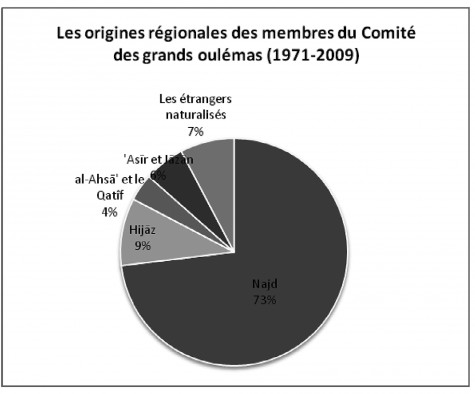
\includegraphics[width=4.94996in,height=4.10417in]{Image/media/image11.jpeg}

18 Une majorité des membres du Comité des grands oulémas est donc
\emph{najdī} et ce depuis sa création. Deux remarques pourraient être
faites à ce propos. La première est que si l'on peut aisément comprendre
que seuls 4\% des grands oulémas sont des Aḥsā'ī-s puisque une grande
partie de la population de cette province est chiite ou sunnite autres
que hanbalo-wahhabite; si l'on peut aussi comprendre que seuls 9\% des
grands oulémas sont \emph{ḥijāzī} puisque, bien que sunnites, ils ne
sont, généralement, pas hanbalo- wahhabites, le chiffre de 6\% seulement
d'oulémas originaires du Sud de l'Arabie Saoudite peut, du moins \emph{a
priori}, paraître absurde puisque les habitants de cette région sont en
majorité hanbalo-wahhabites. L'hypothèse de la préférence régionale peut
être ainsi raisonnablement soutenue: si 73\% des grands oulémas sont
\emph{najdī}, c'est, justement, parce qu'ils sont originaires du fief du
hanbalo-wahhabisme et de la maison
des Sa‛ūd et que, de ce fait, leur soumission à l'un et à l'autre ne
peut être remise en cause. La seconde remarque est que si l'on compare
les chiffres avancés pour le Comité des grands oulémas à ceux que
présente le conseil des ministres au sein duquel les Najdī constituent
72\% des membres (Ibn Ṣunaytān, 2004: 70-73); à ceux du Conseil
consultatif où les Najdī sont majoritaires à 51\% (\emph{ibid}.: 93-96);
à ceux des ministres plénipotentiaires qui sont à 78\% originaires du
Najd ou encore, à ceux des hauts fonctionnaires qui comptent 67\% de
Najdī (\emph{ibid}.: 177-178), on voit que l'élite saoudienne étatique,
qu'elle soit religieuse ou politique, est majoritairement \emph{najdī}.
Les gens du Sud, eux, qui, comme on l'a dit, sont majoritairement
hanbalo-wahhabites, ne représentent que 1\% des ministres, 7\% des
membres de Conseil consultatif, moins de 5\% des ministres
plénipotentiaires et moins de 9\% des hauts fonctionnaires
(\emph{ibid}.: 177- 178): le même raisonnement peut être, ici,
développé. Le régionalisme primerait en Arabie Saoudite. Même si l'on
parle de saoudisation et de formalisation, l'État continue toujours de
s'appuyer sur l'élément najdo-wahhabite pour fonctionner.

19 Observons les chiffres de plus près: lorsque 9\% seulement des
oulémas sont originaires du Hijâz, 20\% des membres du conseil des
ministres, 29\% des membres du Conseil consultatif, 22\% des hauts
fonctionnaires sont \emph{ḥijāzī} (et 34\% parmi eux des cadres
supérieurs). Par ailleurs, en observant les chiffres de plus près
encore, il apparaît qu'au moment de la création du Comité, 29\% des
oulémas sont originaires du Hijâz contre 9\%, nous l'avons dit,
aujourd'hui. Le Comité tend donc, au fur et à mesure qu'il se met en
place et qu'il n'a plus besoin de cadres supérieurs, à se fermer à tout
ce qui n'est pas \emph{najdī}. Il faut ajouter à cela que les oulémas,
quand ils ne sont pas hanbalo- wahhabites, dissimulent leurs croyances
-- ou du moins évitent d'en parler -- et ne jouent, une fois admis au
sein du Comité, qu'un rôle de «figurants».

20 Le Comité des grands oulémas voudrait donner une illusion
d'ouverture: les principales régions sont toutes, même à une faible
proportion, «représentées». Actuellement, deux oulémas d'origine
\emph{ḥijāzi}, deux oulémas originaires du Sud et un autre de l'Est sont
membres du Comité des grands oulémas. En réalité, l'élément \emph{najdī}
domine toujours le Comité, et de loin; de plus, en supposant qu'il y ait
ouverture et même si le Comité accepte en son sein des chiites, il lui
suffirait de conserver une majorité de 51\% de hanbalo-wahhabites
(Najdī) pour que le vote à la majorité absolue passe au sein du Comité
et qu'ainsi, la vision hanbalo-wahhabite continue à dominer.

21 Enfin, en ce qui concerne les oulémas d'origine étrangère, ils ne
sont admis au sein du Comité (au nombre de trois) qu'au moment de la
création de ce Comité. Ces oulémas étrangers étaient, en effet, plus
compétents et plus qualifiés que les oulémas locaux; ils étaient dévoués
à l'État et au hanbalo-wahhabisme; nés non-wahhabites, ils l'étaient
devenus par conviction; ils n'avaient pas d'assise sociale et tribale en
Arabie Saoudite et devaient leur ascension à l'État; enfin, la
solidarité islamique, initiée par le roi Fayçal, entrait également en
ligne de compte. Depuis, le Comité s'est fermé aux étrangers et même les
enfants des dits oulémas étrangers ne sont pas admis au sein du Comité.

22 Le tracé reliant les villes du Najd dont les grands oulémas sont
originaires forme,
pour ainsi dire, un croissant que nous conviendrons d'appeler «croissant
\emph{najdī}» et qui constitue l'épicentre de l'Arabie Saoudite en même
temps que celui du hanbalo- wahhabisme. Il ne faut toutefois pas croire
que si les oulémas du Najd sont largement majoritaires au sein du
Comité, toutes les villes et les régions du Najd y seront équitablement
«représentées». Le Najd compte trois principales régions: la région de
Riyad qui a donné vingt-sept oulémas, le Qaṣīm dix et le Ḥā'il qui n'a
donné aucun \emph{`ālim}. Les deux régions, de Riyad et du Qaṣīm,
offrent un quasi-équilibre dans la répartition des oulémas: dans la
région de Riyad, en dehors de la ville elle-même, qui donne, à elle
seule, sept oulémas, les autres villes donnent, chacune, entre un et
quatre oulémas. De même, dans la région du Qaṣīm, le nombre d'oulémas
par ville varie entre un et trois.

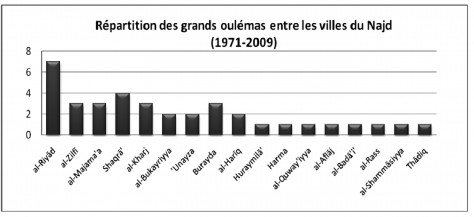
\includegraphics[width=4.9375in,height=2.26042in]{Image/media/image12.jpeg}

23 Le Ḥā'il, quant à lui, est volontairement marginalisé pour une raison
historique évidente: l'émirat du Ḥā'il a longtemps été le rival direct
des Saoud. Nous retrouvons à peine un représentant de cette région dans
le conseil des ministres et un seul autre au Conseil consultatif (Ibn
Ṣunaytān, 2004: 71 et 94).

24 Notons, pour finir, que certaines régions du Najd sont totalement
exclues et n'ont donné aucun \emph{`ālim}: l'exemple d'al-Dawādimī, pour
ne citer que lui, explique ce phénomène dans la mesure où la plupart des
habitants de la ville sont issus de la tribu des `Utayba dont la
fidélité au régime est douteuse. Il y aurait ainsi sous-régionalisation
à l'intérieur même de la régionalisation. De même, aucun grand
\emph{`ālim} n'est issu des régions du Nord. Enfin, aucun chiite n'est
admis au Comité des grands oulémas et ce, pour des raisons évidentes
qu'il ne semble pas utile de rappeler ici. Cela dit, les acquis familial
et tribal, seuls, ne suffisent pas: l'apprenti grand \emph{`ālim} doit
encore suivre un cursus d'études particulier pour intégrer le Comité.
\end{quote}

\hypertarget{de-la-ijux101za-au-doctorat-institutionnalisation-de-la-formation-du-ux101lim}{%
\section{\texorpdfstring{De la \emph{ijāza} au doctorat,
institutionnalisation de la formation du
‛ālim}{De la ijāza au doctorat, institutionnalisation de la formation du ‛ālim}}\label{de-la-ijux101za-au-doctorat-institutionnalisation-de-la-formation-du-ux101lim}}

\begin{quote}
25 Sur les cinquante-deux oulémas qui ont été membres du Comité des
grands oulémas depuis sa création, en 1971, 22\% (soit treize oulémas)
ont reçu une formation traditionnelle et 78\% (soit trente-neuf oulémas)
une formation «moderne». Près d'un quart des oulémas sont ainsi passés
par un cursus traditionnel. Nos entretiens nous permettent de décrire ce
\emph{ta‛līm} et d'en ressortir avec le cursus traditionnel «idéal
typique» du \emph{`ālim} hanbalo-wahhabite.

26 Au départ, entre l'âge de cinq et sept ans, l'apprenti \emph{`ālim}
fait son apprentissage du Coran. Les apprentis oulémas issus d'un milieu
modeste, ceux qui seront plus tard des self-made-men, apprennent le
Coran dans une école coranique (\emph{al-kuttāb}), aux mains d'un cheikh
de renommée moyenne. Les enfants des «cadres religieux moyens» et les
rejetons des dynasties d'oulémas, eux, apprennent le Coran auprès de
leur père, de l'un des membres de leur famille, ou d'un précepteur. On
imagine bien les difficultés rencontrées par les apprentis grands
oulémas issus de milieux modestes et le décalage qui se marque, dès le
départ, entre les apprentis oulémas issus des différentes classes
sociales.

27 Après cette phase d'apprentissage du Coran, l'apprenti \emph{`ālim}
doit, d'une part, commencer à étudier la grammaire et la rhétorique
arabes, de l'autre, apprendre par cœur les trois principaux ouvrages
d'Ibn `Abd al-Wahhāb sur l'unicité divine (\emph{al- tawḥīd}),
fondements du hanbalo-wahhabisme.

28 La troisième étape du cursus classique de l'apprenti \emph{`ālim} est
la quête du savoir
auprès des oulémas réputés. Le futur grand `ālim doit, en effet, réunir
un grand nombre de \emph{ijāzāt} (pl. de \emph{ijāza}: licences), dans
toutes les branches du savoir islamique disponibles, notamment en droit
et en théologie. Il assiste, pour ce faire, plus ou moins
assidûment, à des \emph{ḥalaqāt} `\emph{ilmiyya} ou cercles de savoir,
organisés quotidiennement dans les mosquées ou aux domiciles des
oulémas. Il s'agit alors, de séances de lectures mécaniques suivies de
commentaires d'ouvrages de hadith, d'exégèse coranique, de droit et de
théologie, notamment l'étude des œuvres classiques hanbalites. C'est à
l'issue de ces \emph{ḥalaqāt}, et une fois que l'étudiant a bien retenu
l'ensemble de l'enseignement dispensé par le \emph{`ālim}, qu'il fait un
\emph{istid`ā'}: une demande d'\emph{ijāza} pour les ouvrages étudiés.
Les étudiants les plus brillants deviennent assistants du maître et cela
leur ouvre la porte pour devenir professeur ou juge: la carrière est
alors lancée. Cela a été le cas de Muḥammad al-Sbayyil, le dernier grand
\emph{`ālim} à avoir reçu une formation traditionnelle.

29 Né dans la région du Qaṣīm vers 1926, al-Sbayyil est issu d'une
famille de «cadres religieux moyens». Son père, libraire et copiste
d'ouvrages religieux, connaît parfaitement le Coran. Son frère aîné,
`Abd al-`Azīz, est un \emph{`ālim} de la ville d'al- Bukayriyya. À l'âge
de cinq ans, al-Sbayyil commence son apprentissage du Coran auprès de
son père puis de son frère. Vers l'âge de dix ans, il se lance dans
l'apprentissage des trois ouvrages fondamentaux d'Ibn `Abd al-Wahhāb. Il
étudie aussi la jurisprudence hanbalite sous la direction des oulémas du
Qaṣīm, notamment les ouvrages d'Ibn Taymiyya (m. 1328), d'Ibn Qayyim
al-Jawziyya (m. 1350) et de Mar`ī al- Karamī (m. 1624), etc. À l'âge de
vingt ans, il aurait déjà acquis plusieurs \emph{ijāzāt} qui lui
permirent de devenir l'assistant du juge du Qaṣīm, `Abd Allāh b. Ḥumayd.

30 La formation traditionnelle indispensable au tout début du e siècle
perd, peu à peu, du terrain. En effet, les oulémas qui ont reçu cette
formation s'adaptent difficilement aux exigences de la modernité. 53\%
des membres du Comité des grands oulémas, soit neuf oulémas, ont reçu,
en 1971, une formation dite traditionnelle; en 2009, aucun grand
\emph{`ālim} ne bénéficie d'une telle formation. Dans un pays qui tente
de se moderniser, le besoin d'uniformisation de la formation des grands
oulémas s'impose. Il a fallu, pour y répondre, créer un cursus complet,
homogène, un cursus «national». Nous entendons par cursus moderne, un
cursus «institutionnalisé» et uniformisé.

31 S'ils ne sont que 47\% (soit huit oulémas), en 1971, à suivre la
formation dite moderne,

ils sont aujourd'hui 100\% à le faire. Après un cycle d'études primaires
dans des écoles publiques2\emph{,} les élèves qui se destinent à faire
une carrière juridico-religieuse, rejoignent les instituts de sciences
religieuses (\emph{al-ma`āhid al-`ilmiyya}). Le premier institut voit le
jour à Riyad, en 1950, à l'instigation du grand mufti du royaume de
l'époque, Muḥammad b. Ibrāhīm. Mais très vite, le gouvernement adopte le
projet et les instituts fleurissent dans toutes les régions du royaume
pour atteindre le chiffre de soixante- deux en 2009. Pour accéder à
l'enseignement de ces instituts, l'enfant doit avoir un dossier correct
et avoir appris au moins deux parties du Coran. L'enseignement y est
gratuit. Les instituts de sciences religieuses proposent un cursus de
six années: trois années de collège sanctionnées par un certificat de
réussite, sorte de «brevet» et trois années de lycée sanctionnées par un
certificat de réussite, sorte de «baccalauréat». Les matières étudiées
ont évolué depuis les années cinquante. Au début, l'enseignement était
constitué de quatre troncs communs: les sciences religieuses, les
sciences de la langue arabe, les «sciences sociales», et les
mathématiques. Au fil des années, on a ajouté à ce tronc commun d'études
de base, l'apprentissage obligatoire de la langue anglaise et de
l'informatique. Ces instituts de sciences religieuses sont inégalement
répartis sur l'ensemble du pays: le Najd compte 34\% des instituts, le
Hijâz 13\%, le Sud 28\%, le Nord 18\%, l'Est, enfin, 7\%. Les instituts
sont nombreux dans les régions où le hanbalo-wahhabisme est majoritaire
c'est-à-dire dans le Najd, le Sud et le Nord.

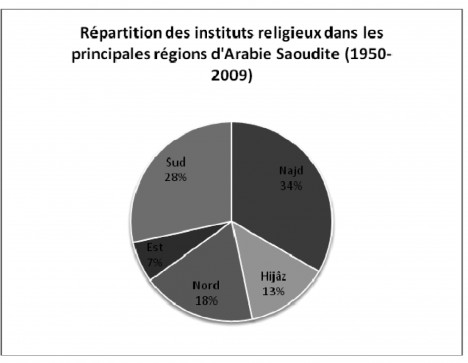
\includegraphics[width=4.875in,height=3.78125in]{Image/media/image13.jpeg}

32 Si la proportion entre le nombre d'instituts créés dans le Hijâz et
celui des oulémas qui sont admis au Comité des grands oulémas est
relativement équilibrée, la proportion entre le nombre d'instituts créés
dans les trois autres régions hanbalo-wahhabites et celui des oulémas
issus de ces régions et effectivement admis au sein du Comité, est,
quant à elle, largement déséquilibrée. On s'attendrait, en effet, à un
nombre plus important d'instituts de sciences religieuses dans le Najd,
à un nombre moins important dans le Sud et à un nombre nul d'instituts
dans la région du Nord. Or, ils sont créés dans le Nord et dans le Sud
mais ce, moins dans le but de former des grands oulémas que dans celui
de «wahhabiser» ces régions en y formant des techniciens du culte
hanbalo-wahhabite et des «cadres religieux moyens».

33 Lorsque l'apprenti \emph{`ālim} a terminé avec succès ses études
secondaires au sein de l'institut, il peut postuler pour les trois
grandes universités du pays: l'Université islamique de Médine (al-Jāmi`a
al-islāmiyya), l'Université islamique de la Mecque (Jāmi`at Umm al-Qurā)
et l'Université islamique de Riyad (Jāmi`at al-imām Muḥammad b. Sa`ūd
al-islāmiyya).

34 La première de ces universités, fondée en 1961, accueille surtout les
musulmans étrangers. Les Saoudiens qui y étudient se destinent
généralement à la prédication à l'étranger. De cette université n'est
issu qu'un seul grand \emph{`ālim}.

35 Quant à la deuxième citée, elle est la plus ancienne université de
théologie d'Arabie Saoudite, fondée en 1949. Elle n'a, malgré son
ancienneté, donnée que six grands oulémas. Doit-on y voir une
manifestation du régionalisme saoudien? Toujours est-il que cette
université accueille, depuis les années soixante-dix, des professeurs,
des cadres et des étudiants de diverses tendances politico-religieuses,
notamment des frères musulmans et des sahwistes (Lacroix, 2010: 47-97)
en lesquels le gouvernement saoudien et le Comité des grands oulémas
n'ont que très peu confiance et qui ne sont donc pas spontanément
recrutés par celui-ci.

36 La dernière université, enfin, est incontestablement la plus
importante pour notre étude. Elle a donné vingt-cinq oulémas, soit 51\%
des membres du Comité, depuis sa création en 1971, et 75\% des oulémas
ayant fait des études universitaires modernes. Cette université naît, en
1974, de la fusion de la faculté de théologie créée, elle, en 1953, et
de la faculté de langue arabe, créée en 1954.

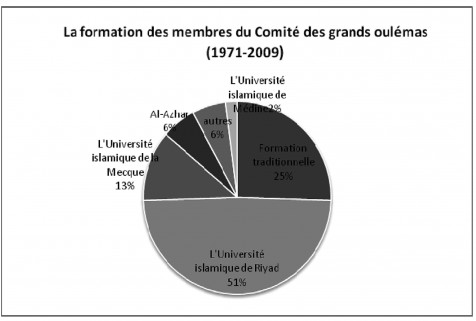
\includegraphics[width=4.95833in,height=3.34375in]{Image/media/image14.jpeg}

37 Depuis sa création, l'Université islamique de Riyad, qui,
rappelons-le, porte le nom du fondateur de l'émirat saoudien Muḥammad b.
Sa`ūd (1744-1765), fidèle allié d'Ibn `Abd al-Wahhāb, est considérée
comme le vivier des grands oulémas et de tous les cadres religieux et
techniciens du culte dont l'establishment religieux a besoin. Le

«pharaonique» campus de l'université (une véritable ville dans la ville
avec ses propres infrastructures, un petit hôpital, un supermarché, des
quartiers résidentiels pour les étudiants, les professeurs et le
personnel administratif, etc.) compte neuf facultés et deux instituts
supérieurs: la faculté de droit {[}musulman{]}; la faculté de théologie;
la faculté de langue arabe; la faculté des sciences sociales
{[}islamiques{]}; la faculté de la prédication et de la communication;
la faculté des langues et de la traduction; la faculté des sciences de
l'informatique; la faculté de l'économie; la faculté des sciences;
l'Institut supérieur de la magistrature et l'Institut de l'apprentissage
de la langue arabe {[}pour les étrangers{]}. Cela dit, les grands
oulémas sont exclusivement issus des facultés de droit et de théologie
et de l'Institut supérieur de la magistrature. Les étudiants dans ces
trois domaines bénéficient d'une bourse d'études et obtiennent, dès la
fin de leur première année d'études, le titre fort apprécié de
\emph{shaykh}. Le succès de l'Université islamique de Riyad est tel que
celle-ci s'est engagée dans une politique d'expansion en développant
deux filiales en Arabie Saoudite3 et cinq à l'étranger4\emph{.} Enfin,
certains étudiants peuvent préparer leur doctorat en sciences
religieuses à l'université égyptienne d'al-Azhar, pour le prestige que
cela donne. Une autre raison pourrait être avancée: certains apprentis
oulémas saoudiens iraient à al-Azhar pour observer l'organisation, les
structures et les mécanismes de fonctionnement de cette prestigieuse
université en vue de les
«importer» en Arabie Saoudite.

38 Les oulémas, au moment de leurs études supérieures, ont tous un tronc
commun tripartite: les fondements de la théologie (\emph{al-`aqīda});
l'exégèse coranique (\emph{al tafsīr}) et la jurisprudence
(\emph{al-fiqh}). À partir de la première année de master (calqué sur le
système anglo-saxon), 74\% des oulémas se spécialisent dans la
jurisprudence, et plus spécialement dans les fondements de la
jurisprudence islamique (\emph{uṣūl al-fiqh}) dans le but d'acquérir la
qualification requise pour émettre des \emph{fatwā}; 26\% d'entre eux,
se spécialisent en théologie, et plus précisément en religions comparées
(en réalité, pour dénigrer toute autre religion que l'islam
hanbalo-wahhabite)5\emph{.} Le choix de ces spécialisations n'est pas
étonnant dans la mesure où les étudiants se destinent avant tout à être
des techniciens du culte et des gestionnaires des biens de salut. Nous
n'entrerons pas, pour ne pas alourdir notre propos, dans le détail des
spécialisations pointues à l'intérieur même des deux grands domaines de
spécialisations que nous avons évoqués.

39 Bien que le cursus moderne se soit bien implanté dans le paysage
saoudien, l'ijāza
n'en demeure pas moins source de prestige et un élément non négligeable
dans un
capital social. Nous avons pu observer que la totalité des oulémas qui
ont suivi le cursus moderne ont, néanmoins, obtenu une ou plusieurs
\emph{ijāzāt}. Elément de prestige comme nous venons de le dire,
l'\emph{ijāza} est, en théorie, facultative. Mais, en pratique,
l'obtention d'une \emph{ijāza} permet au \emph{`ālim}, d'une part, de se
rattacher à une chaîne de transmission
«ininterrompue» d'oulémas remontant jusqu'au Prophète, ce qui permet au
\emph{`ālim} de légitimer sa position et son savoir et de s'inscrire
dans l'héritage prophétique, d'autre part, de nouer des relations
privilégiées avec un ou plusieurs oulémas et de commencer ainsi à tisser
un réseau qui pourra le mener au sommet de l'establishment hanbalo-
wahhabite.

\textbf{Faire carrière: le \emph{cursus honorum} des oulémas}

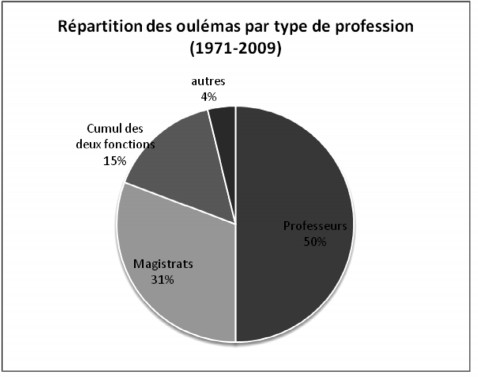
\includegraphics[width=4.97917in,height=3.92708in]{Image/media/image15.jpeg}40
L'enseignement et la magistrature ont toujours été les métiers de
prédilection des oulémas. Les membres du Comité des grands oulémas
n'échappent pas à cette règle. 96\% d'entre eux exercent au moins une de
ces deux professions: 50\% du Comité, soit vingt et un grands oulémas,
ont été ou sont encore, professeurs de jurisprudence islamique ou de
théologie; 31\% d'entre eux sont magistrats dans les différentes
instances de la justice saoudienne; 15\% des grands oulémas ont cumulé
les deux fonctions. À la question: «pourquoi le choix de ces métiers?»
Une première réponse, unanime, des grands oulémas magistrats: «la
justice est le fondement de la royauté». Et, selon les oulémas, qui,
mieux que des spécialistes de «la loi divine», pourraient mettre la
justice en application! Les grands oulémas ont d'ailleurs pleine
conscience de l'importance de leur mission. Ils ont une vision
catastrophiste d'un monde où le \emph{`ilm}, qui risque d'être perdu,
doit être sauvé, épuré des innovations blâmables et transmis par le
\emph{`ālim}.

41 En outre, si la magistrature permet au grand \emph{`ālim} d'observer,
d'analyser et de statuer sur des cas concrets, l'enseignement permet de
transmettre le savoir théorique. Cela, en plus du prestige qui entoure
ces deux fonctions. Il n'est, enfin, pas étonnant de voir que nombre de
grands oulémas cumulent les deux fonctions puisqu'en réalité, l'une et
l'autre sont indissociables (pratique et théorie). Ce phénomène de cumul
des fonctions (d'enseignant et de magistrat) est surtout visible dans la
première génération des grands oulémas. Il s'explique par le manque de
cadres religieux au moment de la
création du Comité. Les grands oulémas devaient donc assumer, tout à la
fois, leur rôle au sein du Comité et les fonctions de magistrats et
d'enseignants. Des années quarante aux années soixante, l'Arabie
Saoudite a été obligée d'«importer» des cadres religieux de l'étranger,
notamment de l'Égypte. Un exemple: l'Égyptien `Abd al-Razzāq `Afīfī (m.
1994), arrivé en Arabie Saoudite, en 1949, pour enseigner la langue
arabe et les sciences religieuses dans un collège à Tayef, a gravi, un à
un, les échelons et parvient au sommet de l'establishment religieux: il
est nommé, en 1971, au sein du Comité des grands oulémas. Cet exemple
révèle deux réalités: premièrement, l'Arabie Saoudite a fait appel aux
étrangers pour l'enseignement, à une certaine époque, à cause du déficit
de cadres dont elle a souffert dans tous les domaines; et deuxièmement,
les étrangers hanbalo-wahhabites, qui pouvaient aisément s'intégrer dans
le pays d'accueil, ont pu, à force de persévérance, atteindre le sommet
de l'establishment religieux saoudien.

42 La pratique du cumul des fonctions d'enseignant et de magistrat tend
à disparaître: le dernier grand \emph{`ālim} à avoir cumulé ces deux
fonctions est `Abd Allāh b. Qa`ūd, membre du Comité de 1977 à
19866\emph{.} Désormais, les grands oulémas, qu'ils soient professeurs
ou magistrats, sont de plus en plus spécialisés, chacun dans son
domaine: de professeurs de droit en général, ils sont devenus
professeurs de droit pénal, de droit de la famille, etc. Parallèlement à
ces deux métiers de prédilection, les grands oulémas sont techniciens du
culte: la plupart d'entre eux sont imâm dans les mosquées. Par exemple,
le grand mufti actuel du royaume, `Abd al-`Azīz āl al-Shaykh, est
également imâm de la grande mosquée de Riyad. Sāliḥ b. Ḥumayd est, lui,
imâm de la grande mosquée de la Mecque, etc. N'oublions pas enfin,
l'autre fonction essentielle des grands oulémas, celle d'«entrepreneurs»
de biens de salut, à savoir promulguer des \emph{fatwā} et se mettre à
l'écoute de la population. Mais si les grands oulémas monopolisent les
grands postes religieux et judiciaires saoudiens, ils n'hésitent pas à
empiéter sur le domaine réservé des autres élites.

43 Une fois admis au sein du Comité, le grand \emph{`ālim} obtient
automatiquement le grade de haut fonctionnaire (\emph{al-martaba
al-mumtāza}), voire celui de ministre. Sur les cinquante-deux membres du
Comité des grands oulémas, vingt-deux ont occupé des postes de
responsabilité autres que ceux de magistrats et d'enseignants. Déjà neuf
membres de la \emph{Hay'a} ont été ou sont encore ministres. Les
ministères que contrôlent les oulémas (si ce ne sont pas eux qui les
contrôlent directement, c'est un membre de l'establishment religieux)
sont ceux de la justice, des affaires islamiques, du pèlerinage et de
l'enseignement des filles (avant le rattachement de ce dernier, en 2002,
au ministère de l'éducation nationale). Depuis sa création, le ministère
de la justice est dirigé par un membre du Comité7\emph{.} Huit membres
du Comité des grands oulémas on été membres du Conseil consultatif: le
président de ce conseil, qui fait se côtoyer islamistes,
«libéraux», conservateurs et tribaux, depuis sa création, en 1992, est
un membre du Comité des grands oulémas. De 1992 à 2002, c'est Muḥammad
b. Jubayr, membre du Comité des grands oulémas (de 1971 à 2002), qui
assure la présidence de cette instance. Sāliḥ b. Ḥumayd, membre du
Comité des grands oulémas depuis 2001, lui succède en 2002. Ce dernier
est remplacé par `Abd Allāh Āl al-Shaykh, en 2009. Trois membres de la
\emph{Hay'a} ont été conseillers du roi Fahd (1982-2005) et deux sont
actuellement conseillers du roi `Abd Allāh. Quatre membres du Comité ont
occupé les postes de doyen ou de président d'université. Par exemple,
`Abd al-`Azīz b. Bāz occupe jusqu'à sa mort, en 1999, le poste de
président de l'Université islamique de Médine. Sa`d al- Ḍuwayḥī est
doyen de la faculté de théologie d'al-Aḥsā'. `Abd Allāh b. `Abd
al-Muḥsin al- Turkī, sans doute l'un des membres les plus actifs du
Comité, actuellement, occupe le poste de président de la Ligue islamique
mondiale, après avoir occupé, entre autres, les postes de président de
l'Université de Riyad et de ministre des affaires islamiques.

44 C'est dire que les oulémas ont adopté, depuis au moins deux
décennies, une stratégie adaptative qui les pousse à investir plusieurs
secteurs d'activités. Outre les domaines religieux, législatif et
éducatif, ils investissent les associations caritatives, les
organisations gouvernementales et non gouvernementales et les domaines
économique et financier. Dans ces deux derniers domaines, trois oulémas,
`Abd Allāh b. Manī`, `Abd
al-Wahhāb Abu Sulaymān et `Abd Allāh al-Muṭlaq se sont «improvisés»
experts et consultants incontournables dans les marchés financiers
saoudiens. Les trois hommes sont aussi membres de plusieurs conseils
d'administration de banques et d'entreprises dans le cadre de ce que
l'on appelle en Arabie Saoudite \emph{al-lijān al-šar`iyya} ou
commissions islamiques. Le nom-même d'un grand \emph{`ālim} sur la
brochure d'une société ou d'une entreprise est la meilleure des
publicités.
\end{quote}

\hypertarget{la-multiplication-des-ruxe9seaux-de-soutien}{%
\section{La multiplication des réseaux de
soutien}\label{la-multiplication-des-ruxe9seaux-de-soutien}}

\begin{quote}
45 Cette mobilité des oulémas n'est, toutefois, possible que si le
\emph{`ālim} tisse, autour de lui, un réseau sur lequel il peut
s'appuyer. Les capitaux culturel et économique doivent encore être
complétés par un réseau de soutiens. Nous avons pu observer trois types
de capitaux sociaux mobilisés par le futur grand \emph{`ālim}. Autrement
dit, le recours aux relations personnelles permet à ce dernier de
s'assurer une meilleure position dans la hiérarchie sociale. Ces trois
réseaux, que nous exposons séparément, sont en réalité, presque
toujours, combinés par le futur grand \emph{`ālim}. Le réseau familial
constitue la première ressource du futur grand \emph{`ālim}. Nous avons,
en effet, constaté l'existence d'au moins trois exemples de réseaux
familiaux qui sont autant de moyens d'accès au Comité des grands
oulémas.

46 Le premier est, sans aucun doute, le plus puissant et le plus dense:
celui des Āl al- Shaykh. Nous avons évoqué plus haut l'importance de
cette famille et nous tenterons, dans ce qui suit, de compléter le
tableau amorcé. L'exemple des deux fils, Ibrāhīm et `Abd Allāh, du grand
mufti Muḥammad b. Ibrāhīm est tout à fait significatif: bien que le
premier des deux ait été relativement peu brillant par rapport aux
collaborateurs de son père, il a quand même été nommé par ce dernier
vice-mufti du royaume d'Arabie Saoudite. Après la mort de son père et la
suppression du poste de mufti, Ibrāhīm, qui était destiné à devenir
mufti, reçoit, en guise de consolation, les postes de ministre de la
justice, de membre du Comité des grands oulémas et de président de la
Direction de la recherche scientifique, de la prédication et de
l'instruction! En 1992, lorsqu'Ibrāhīm se retire des affaires, son
remplaçant au ministère et au Comité des grands oulémas n'est autre que
son frère cadet `Abd Allāh, président actuel du Conseil consultatif. Un
autre exemple étonnant de la famille Āl al-Shaykh: il s'agit de Ṣāliḥ b.
'Abd al-`Azīz, le petit fils d'Ibn Ibrāhīm. Après avoir fait des études
scientifiques depuis le lycée et obtenu un diplôme d'ingénieur, Ṣāliḥ
décide de récupérer l'héritage familial et s'inscrit à l'Université
islamique de Riyad. Grâce à son nom et à l'intervention de son père, qui
était l'un des conseillers du roi Fahd, il obtient une équivalence et
passe ainsi directement en année de master: il contourne la règle qui,
aussi stricte soit-elle, s'efface quand il s'agit d'un Āl al-Shaykh. Il
est actuellement ministre des affaires islamiques et, potentiellement,
membre du Comité des grands oulémas. Un dernier exemple enfin de cette
famille: le dernier admis à Hay'at kibār al-'ulamā', Muḥammad b. Ḥasan,
fait une ascension fulgurante grâce à ses bonnes relations avec son
cousin, le grand mufti actuel d'Arabie Saoudite: il a pu, rapidement,
gravir les échelons universitaires et devenir le directeur de cabinet du
mufti. Ce dernier l'épaule et le soutient: il propose son nom au Comité
des grands oulémas auquel Muḥammad b. Ḥasan accède en avril 2005.
Signalons, enfin, que le réseau familial des Āl al-Shaykh et l'influence
qui en découle, dépassent largement le seul cadre religieux: un membre
de la famille est ambassadeur à Paris, un autre est directeur du
protocole royal, un troisième est membre de la chambre de commerce, etc.
Le deuxième réseau familial est celui des Ibn Ḥumayd, déjà présenté plus
haut.

47 Le dernier réseau familial, enfin, de moindre importance, est celui
des al-Šathrī: cette
famille du Najd a donné quelques oulémas et plusieurs hommes politiques.
`Abd al-‛Azīz al-Šathrī, un des conseillers des rois Fayçal (1964-75) et
Ḫālid (1975-82) a également été un ouléma de renommée moyenne. Son fils,
Nāṣir, a réussi à faire une brillante carrière politique (en tant que
conseiller des rois Ḫālid et Fahd). Selon un des
membres du clan al-Šathrī: «il ne manquait à {[}la{]} famille qu'un
grand \emph{`ālim} pour qu'{[}elle{]} devienne, enfin, une grande
famille». La parentèle met tout en œuvre pour que son rejeton prodige,
Sa‛d, accède au sommet de l'establishment religieux. Aussi, le
prépare-t-on, dès son plus jeune âge, à devenir grand \emph{`ālim} : on
le confie aux maîtres les plus compétents dans le domaine, tels Ibn Bāz,
Ibn `Uthaymīn, al-Aṭram, al-Rakbān et `Abd al-`Azīz Āl al-Shaykh. On le
pousse à s'inscrire à Jāmi'at al-imām où il obtient un doctorat en
fondements de la jurisprudence islamique. Sa`d brûle toutes les étapes
du \emph{cursus honorum} hanbalo-wahhabite et devient professeur de la
même université en un temps records. En mars 2005, la famille soutient
la candidature de son fils au Comité des grands oulémas (le père est
membre du cabinet royal qui transmet les candidatures au roi). Sa`d est
finalement nommé, en avril 2005: à trente-huit ans, il est le plus jeune
membre de l'histoire du Comité des grands oulémas.

48 Nous l'avons dit, le régionalisme et le segmentarisme dominent le
paysage politico- religieux saoudien. La deuxième ressource du futur
grand \emph{`ālim} est, naturellement, le réseau tribal qui va de pair
avec le réseau régional, autrement dit avec le réseau \emph{najdī}. Nous
avons remarqué, en analysant les origines géographiques et tribales des
grands oulémas, que ces derniers sont généralement issus des plus
grandes confédérations tribales du Najd: les Banū Ḫālid ont donné quatre
grands oulémas, les Banū Zayd, sept, les Banū Subay`, trois, les Banū
Tamīm, huit (auxquels il faut ajouter les quatre grands oulémas des Āl
al-Shaykh), les Qaḥṭān, trois, les `Unayza, trois, les Bāhila, deux et
al- Dawāsir, deux également. Soit un total de trente-six grands oulémas
issus des grandes tribus du Najd sur les cinquante-deux membres du
Comité. Le réseau tribal est très dense. Le nombre de grands oulémas est
plus ou moins bien réparti entre les grandes tribus \emph{najdī}. D'un
mouvement de nomination au sein du Comité à l'autre, cet équilibre est,
consciemment ou inconsciemment, maintenu. Exemple: les deux grands
oulémas, Muḥammad āl Sulaymān et Bakr Abū Zayd, de la tribu des Banū
Zayd -- admis tous deux au Comité, en 1992 -- sont remplacés, en 2005,
par deux hommes issus de la même tribu, `Alī al-Ḍuwayḥī et `Abd
al-Raḥmān al-Sadḥān. D'ailleurs, le réseau tribal doublé du réseau
régional ne concerne pas uniquement le champ religieux: on retrouve ces
mêmes configurations dans le domaine politico-administratif (Ibn
Ṣunaytān, 2004, 59-62).

49 La dernière ressource du futur grand \emph{`ālim} est la
\emph{mulāzama}: le fait de s'attacher un
long moment à un maître en sciences religieuses, réputé et influent.
Côtoyer un maître pendant plusieurs années permet à l'apprenti grand
\emph{`ālim} de nouer avec lui des relations personnelles qui peuvent
même aboutir au mariage de l'élève avec la fille ou la nièce du maître.
Par exemple, Ṣāliḥ al-Luḥaydān est, pendant plusieurs années, le
disciple favori du grand mufti Muḥammad b. Ibrāhīm. Cette relation
privilégiée lance véritablement la carrière de Ṣāliḥ qui devient le
gendre et le directeur de cabinet du mufti et qui gagne peu en peu en
charisme. Une année seulement après le décès du maître, al-Luḥaydān est
admis au Comité des grands oulémas; il hérite aussi de la fonction de
magistrat; quelques années plus tard, il devient le président du Haut
conseil de la magistrature, poste qu'il occupe jusqu'en février 2009.
Al-Luḥaydān est le doyen du Comité des grands oulémas dont il est membre
depuis 1971. Il en est aussi un des membres les plus influents. Il
serait, en effet, le seul à pouvoir opposer un veto pour la nomination
d'un nouveau membre: en 2005, il aurait utilisé son veto pour s'opposer
à l'entrée de l'ouléma `Abd al-Muḥsin al-`Ubaykān au Comité.

50 Un autre exemple: Muḥammad al-Sbayyil est le disciple d'Ibn Ḥumayd
alors que
celui-ci est le \emph{qāḍī} d'al-Bukayriyya. Quand Ibn Ḥumayd devient le
\emph{qāḍī} du Qaṣīm, il fait appeler al-Sbayyil à Burayda pour le
désigner professeur et responsable d'un institut de sciences religieuses
de la région. La relation entre les deux hommes est telle que,
lorsqu'Ibn Ḥumayd devient le grand juge du Ḥijāz, il le fait venir à la
Mecque et le nomme imâm de la grande mosquée de la Mecque et
vice-président de l'administration chargée de gérer les deux lieux
saints. Il finit même par en devenir président (jusqu'en 2005) après la
disparition de son protecteur. Depuis son arrivée à la Mecque, il tisse
des
relations étroites avec des oulémas et grands oulémas notamment Ibn Bāz
(qui n'est pas son maître) mais qui finit par lui proposer de devenir
membre du Comité en 1992.

51 Un troisième exemple: c'est également Ibn Bāz qui suit, pas à pas, la
carrière de `Abd
Allāh b. Qa'ūd qui est son meilleur disciple. À la première occasion (le
décès d'Ibn Ḥumayd et de Miḥḍār `Aqīl), Ibn Bāz propose le nom d'Ibn
Qa`ūd au cabinet royal qui le nomme membre du Comité en 1977.

52 Un dernier exemple enfin: le mufti actuel, `Abd al-`Azīz āl
al-Shaykh, en plus du réseau familial que lui confère son nom, bénéficie
du soutien de son maître Ibn Bāz. Il s'agit d'abord d'une question de
solidarité et de reconnaissance: Ibn Bāz est un \emph{mulāzim} du grand
père de `Abd al-`Azīz Āl al-Shaykh, Muḥammad b. `Abd al-Laṭīf. Il aide
donc `Abd al-`Azīz Āl al-Shaykh à devenir professeur à l'université
d'al-Imām, et propose son nom au cabinet royal pour en faire un membre
du Comité des grands oulémas (il le deviendra en 1987). En 1993, Ibn Bāz
devient mufti et désigne `Abd al-`Azīz āl al-Shaykh vice-mufti du
royaume et ce, bien que d'autres grands oulémas soient plus compétents
que lui. En effet, depuis les années soixante et jusqu'à sa mort, en
1999, Ibn Bāz occupe une position-clé dans l'establishment religieux. Il
bénéficie du respect et de la considération des autres grands oulémas et
exerce, de ce fait, une influence autour de lui, tous les grands oulémas
tenant compte de ses conseils et suivant à la lettre ses directives. La
centralité d'Ibn Bāz est ainsi très importante: un grand nombre de
chemins passent par lui. Dix-huit grands oulémas sont ses disciples et
certains d'entre eux lui doivent leur entrée au sein du Comité.
\end{quote}

\hypertarget{le-quiuxe9tisme-politique}{%
\section{Le quiétisme politique}\label{le-quiuxe9tisme-politique}}

\begin{quote}
53 En cherchant à identifier les conditions d'accès au Comité des grands
oulémas à travers le parcours de ses membres, nous avons constaté qu'il
existe deux critères directement liés à la vie politique et sociale:
aucun des grands oulémas n'a de passé politique (c'est-à-dire, une
quelconque manifestation d'opposition au régime: demande de réformes, ou
autres), et aucun \emph{`ālim} n'a jamais critiqué les décisions du
Comité ou de l'un de ses membres et ce, même si ses positions allaient à
l'encontre des décisions officielles.

54 `Abd Allāh Ibn Jibrīn, haut fonctionnaire religieux et candidat
potentiel au Comité des grands oulémas, a été l'un des parrains de la
contestation islamiste des débuts des années quatre-vingt-dix (Kepel,
2003: 335-337; Lacroix, 2007: 371-443). Ces actes constituent une
véritable offense tant pour le régime que pour les grands oulémas. Ces
derniers ne manquent pas, d'ailleurs, de le désavouer publiquement: il
est démis de ses fonctions officielles. Réhabilité par la suite, et bien
que très bon \emph{`ālim}, il ne pourra cependant jamais prétendre au
poste de grand \emph{`ālim} en raison de cette «bavure»: s'étant
ouvertement opposé au gouvernement et ayant participé à des activités
politiques allant à l'encontre des positions officielles, son «rachat»
et son récent soutien au gouvernement ne suffisent pas. Il ressort de
cet exemple que le quiétisme politique des candidats au Comité est un
élément fondamental et un critère-clé de sélection. Tout ce que peut
tolérer le Comité comme engagement politique pour un futur grand
\emph{`ālim} est le soutien aux décisions du pouvoir. `Alī al-Ḍuwayḥī
est l'exemple du \emph{`ālim} engagé politiquement -- en faveur du
régime bien sûr -- qui accède à la Hay'a. En effet, depuis 2001,
al-Ḍuwayḥī, qui dirige la faculté de théologie d'al-Aḥsā', a signé
plusieurs pétitions politiques défendant les programmes scolaires
saoudiens, et se déclarant en faveur de la tenue d'élections
municipales, etc.

55 Quant à `Abd al-Muḥsin al-`Ubaykān, qui a appelé ouvertement le
gouvernement à entreprendre des réformes, entre 1992 et 1994, il a été
marginalisé et démis de ses multiples fonctions: il perd son poste de
juge au tribunal de Riyad et d'imâm de mosquée. Réhabilité, dans les
années 1999-2000, il continue néanmoins à critiquer les décisions de la
Hay'a (surtout celles qui concernent la jurisprudence), et du système
judiciaire. Il émet même des \emph{fatwā} contredisant celles du Comité
des grands oulémas et
tente, pour se rattraper, de promulguer des \emph{fatwā} sur la licéité
du salut du drapeau national, sur la condamnation des sahwistes ou
encore sur l'interdiction du djihâd en Irak pour les Saoudiens. Le
gouvernement a accepté de le réhabiliter mais les oulémas ont opposé un
veto catégorique à l'entrée de ce \emph{`ālim} au Comité. Al-`Ubaykān a,
finalement, été nommé, dans un premier temps, conseiller au ministère de
la justice et membre du Conseil consultatif, avant de devenir l'un des
conseillers du roi, en 2009.

56 Les leaders de la \emph{ṣaḥwa} dans les années quatre-vingt-dix,
Safar al-Ḥawālī, Salmān al-`Awda et Muḥsin al-`Awājī, reconnaissent
eux-mêmes que l'un des critères d'accès au Comité des grands oulémas est
le quiétisme sur les plans politique et sécuritaire et acceptent donc,
du fait de leur très grand engagement politique, de ne pas y prétendre.

«Pour le gouvernement, dit al-Ḥawālī, les grands oulémas doivent être
des hommes apolitiques, des hommes qui ignorent tout de la politique».
Salmān al-`Awda ajoute que

«les futurs membres du Comité doivent être des hommes sans histoire(s)».
Pour Muḥsin al-`Awājī «l'accès au Comité obéit à des critères purement
sécuritaires».

57 Il découle de tout cela le «portrait idéal» du membre du Comité des
grands oulémas:

le grand \emph{`ālim} est hanbalo-wahhabite; il est issu d'une famille
de «cadres religieux moyens» ou d'une «dynastie» d'oulémas; il est issu
d'une grande tribu sédentarisée du croissant \emph{najdī}; il a effectué
des études auprès de maîtres réputés (cela pour le \emph{`ālim} qui suit
une formation traditionnelle) ou dans un \emph{ma`had `ilmī} puis à
l'université al-Imām de Riyad (pour le grand \emph{`ālim} qui a reçu une
formation moderne); il s'est spécialisé en jurisprudence islamique; il
est généralement professeur d'université (al-Imām) ou magistrat; il a en
moyenne vingt-cinq années d'expérience dans le domaine religieux; il
n'est pas engagé politiquement (s'il l'est, il ne doit l'être qu'en
faveur du régime).

58 La moyenne d'âge du grand \emph{`ālim} qui accède au Comité est de
quarante-sept ans. Il y reste en moyenne quinze ans. Et, si les
circonstances d'accès à la Hay'a sont difficiles à déterminer, les
circonstances de départ de la Hay'a sont, elles, tout à fait claires: le
grand \emph{`ālim} quitte le Comité s'il décède, bien évidemment, s'il
est gravement malade ou s'il a commis un acte jugé répréhensible par le
roi -- en 1992, quatre grands oulémas auraient refusé de signer une
\emph{fatwā} et ont été limogés.

59 Le renouvellement des membres du Comité des grands oulémas est
généralement associé à une période de crise ou de transition. Les
renouvellements de 1987 et de 2001 sont des renouvellements de
transition (plusieurs oulémas sont décédés ou gravement malades), les
renouvellements de 1992 et 2005 coïncident avec des moments de crise
(respectivement, les conséquences de la guerre du Golfe et celles du 11
septembre). Depuis la création de la Hay'a, il y a eu reproduction de
l'élite: il ne reste plus de la génération de 1971 que trois membres.
Nous constatons toutefois que l'élite des grands oulémas restreint
l'accès, même à des personnes qui rempliraient toutes les conditions
formelles pour accéder au Comité. Sans doute le prestige d'appartenir au
Comité des grands oulémas ne pourrait que diminuer si l'accès devenait
trop aisé. L'élite du Comité est donc fermée: cinquante-deux membres en
trente-huit ans.
\end{quote}

\hypertarget{conclusion}{%
\section{Conclusion}\label{conclusion}}

\begin{quote}
60 L'habitus, ainsi défini, des grands oulémas, fruit d'un
conditionnement historique et social, est générateur d'un comportement
adapté, consciemment ou inconsciemment, à la logique de l'espace
politico-religieux saoudien: soutenir le pouvoir politique et gérer le
marché officiel des biens de salut. Les larges prérogatives dont dispose
le Comité dans les domaines politique, social et religieux, à côté de sa
fonction fondamentale de bastion idéologique et d'usine à légitimer les
actions du gouvernement, justifient le contrôle par le pouvoir politique
de son ordre du jour et de son budget et conditionnent le choix, très
sélectif, de ses membres. Les grands oulémas, qui se définissent eux-
mêmes comme les oulémas du pouvoir, doivent être acquis au régime. Si
les origines sociales, le parcours éducatif et les réseaux de
socialisation favorisent l'émergence d'une élite fermée et dévouée au
pouvoir, la `\emph{aṣabiyya} régionale y est pour beaucoup. Le

Comité est, à l'instar des autres institutions du pays, trusté par
l'élément \emph{najdī} (plus de 70\% des membres des élites saoudiennes
sont \emph{najdī}): cette région n'est-elle pas le fief du
hanbalo-wahhabisme et de la dynastie régnante? Il s'agit enfin pour les
oulémas d'un dévouement objectif: les intérêts spirituels et temporels
de l'establishment religieux étant intrinsèquement liés à ceux du
régime, si ce dernier était mis à mal, la domination du
hanbalo-wahhabisme sur le territoire saoudien -- très éclectique
religieusement -- serait indubitablement remise en cause.
\end{quote}


\chapter{Le mouvement réformiste (fin XIXe - début XXe)}
  \mn{(07/02/2022)}
 
 
  
  `ABDUH Muhammad, \emph{Rissalat ai Tawhid - Exposé de la religion
  musulmane}, Geuthner, Paris, 1925, trad. fr. et introduction B. Michel
  et Ch. Moustapha Abdel Razik.
  
 
  
  AL-AFGHANI Jamâl ad-Din, \emph{La réfutation des matérialistes},
  Geuthner, Paris, 1942, trad. fr. A.-M. Goichon. Textes divers in:
  \emph{Orient}, 1962, N° 21 p. 89-115, N°22 p. 125-160, N° 23 p. 169-
  198, N' 24 p. 125-152 et \emph{Orient}, 1963, N° 25 p. 141-152.
 


HADDAD, Mohammed \emph{Le réformisme musulman : une histoire critique},
Paris, Mimesis, 2013. HOURANI, Albert \emph{La pensée arabe et
l'Occident,} Groupe Naufal Europe, Paris, 1991.

JOMIER Jacques \emph{Le Commentaire coranique du Manâr}, Maisonneuve,
Paris, 1954.

MERAD Ali \emph{Le réformisme musulman en Algérie de 1925 à 1940. Essai
d'histoire religieuse et sociale}, Paris, Mouton et Cie, 1967.
 \emph{Ibn Bâdis,
commentateur du Coran}, Geuthner, Paris, 1971.

METCALF, Barbara \emph{Islamic Revival in British India 1860-1900},
Princeton University Press, 1982.

TROLL, Christian \emph{Sayyid Ahmad Khân. A Reinterpretation of Muslim
Theology}, Vikas Publ.

House, New Delhi, 1978.



 \section{Introduction : Arrière fond positiviste}
 
 \paragraph{Auguste Comte}
 
 \paragraph{idée de progrès} Évolutionnisme de société. Le progrès est porté par l'occident. Vision des sociétés évoluant vers un mieux, du coup, hiérarchisation des sociétés, entre les sociétés archaïques et celles qui s'appuient sur la Raison et ont dépassé le stade de la religion.
 
 \paragraph{Acceptation des valeurs occidentales} souveraineté du peuple; droits individuels; liberté d'expression. 
 
 \paragraph{Un discours critique de la Religion} 
 
  %-----------------------------------------------------------------------------------
  \section{Les « Occidentalisants »}
  
\paragraph{trois premiers quarts du XIX} jeunes de l'élite de l'empire Ottoman. L'empire cherche à se réformer en introduisant des éléments européeans. L'Empire Ottoman envoie des jeunes en France pour se former.

\paragraph{Tahtawi} Egyptien, a vécu 5 ans en France (1826-1831). A été ensuite dans l'administration ottomane. \textit{L'Or de Paris}\sn{très intéressant à lire}

\paragraph{Khayr ad-din} Caucasien, installé en Tunisie. A vécu à Paris (1852-1856).

\paragraph{Jeunes ottomans} dans le contexte turque. 

\paragraph{Ils notent le désir de progrès} A la différence de Al Wahhab qui est soupçonneux de l'\textit{innovation}, on valorise le changement social : 
\begin{quote}
    quiconque maitrise un art désire inventer quelque chose inconnu auparavant \sn{Or de Paris}
\end{quote}

 
 \paragraph{État}  Sur le plan politique, une compréhension différente de l'État. Dans le cadre classique, l'État doit assurer la justice. Or, ici l'État encadre le progrès de la société. Ils sont convaincus que ce sont les institutions politiques qui sont à l'origine de la force des États occidentaux. Par contre, ils vont être en retrait sur l'approche critique de la religion du positivisme.
 
 \paragraph{les lumières ont émancipé l'Europe de l'obscurantisme chrétien} avec une pointe polémique : les lumières viennent de la philosophie musulmane, et donc adopter les lumières pour les musulmans, ce n'est pas trahir le patrimoine musulman, c'est se le réapproprier. \sn{C'est la pointe de Tariq Ramadan dans les années 1990}.
 
 \paragraph{Principes politiques} Ils vont associer les principes démocratiques au principe de la \emph{Shura}, \textit{consultation}, principe coranique de consultation des notables, reinterprété dans un contexte moderne.
 \begin{Def}[shura]
    \emph{ intention} - consultation
\end{Def} 
 \paragraph{droit musulman} dans un cadre musulman, Il faut moderniser le droit musulman pour qu'il puisse accompagner le développement de la société. Ils pronent une unification du droit, une seule école, moderne et uniforme. Il faut viser à l'éducation des jurisconsultes, dans un cadre moderne. 
  
  %-----------------------------------------------------------------------------------
  \section{Trois grands réformistes}
   
   Après les occidentalisants, qui préfigurent les modernistes, il y a les réformistes que l'on verra à travers trois figures.
   
   \paragraph{Seyyed Ahmad Khan (1817-1898)} Il ne sort pas de nul part, son père est soufi et sa mère a été formé dans une école fondé par Walî Allâh (P \pageref{Theo:waliAllah}). Très grande figure en Inde
   
   \paragraph{Jamal ad-din Al Afghani (1839-1897)} formé en Inde mais action dans l'Empire Ottoman (séjour important en Egypte (1871-79)) et un autre à Paris où il est exilé (1881-1883). C'est un activiste  : revues, société secrète. Son but est de lutter contre la colonisation. Il finit sa vie sous surveillance ottomane.
   

  
   
    \paragraph{Muhammad Abduh} Egyptien, successeur d'Al Afghani. Il a ensuite développé sa propre pensée. 
    \begin{marginfigure}
       \centering
       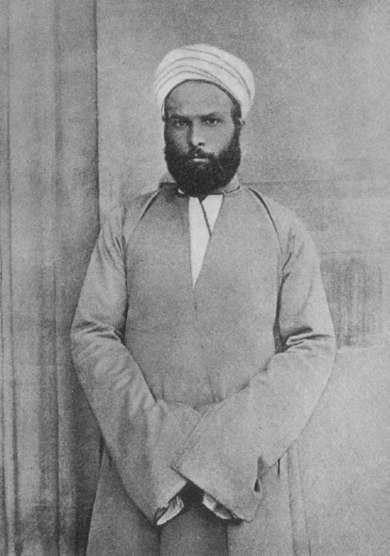
\includegraphics[width=.7\textwidth]{CourantsIslamContemporain/ImagesCourantsIslamContemporain/390px-Muhammad_Abduh.jpg}
       \caption{\href{https://fr.wikipedia.org/wiki/Mohamed\_Abduh}{Muhammad Abduh}}
       \label{fig:my_label}
   \end{marginfigure}
   Surtout en Egypte mais a partagé le séjour parisien de \textit{Aghani} puis au Liban. On lui a interdit d'enseigner mais il a été nommé grand mufti d'Egypte (1899). On avait moins peur de son activité du droit que de son activité sur les jeunes en tant qu'enseignant. Fonde aussi une école qui va évoluer différemment.  
    
    \paragraph{Avancée coloniale plus avancée} La colonisation s'est accentuée : les occidentaux apparaissent comme une menace politique. Peur du colonialisme. Le positivisme s'est aussi accentué. Ils doivent se situer dans le rapport entre Foi et Raison. 
   
   \paragraph{Héritiers du pre-réformisme} En inde en particulier, décadence du monde musulman. beaucoup plus faibles que l'occident, parce que \textit{nous avons perdu l'authenticité de la Foi musulmane}. Pour retrouver notre puissance, il faut retrouver l'authenticité de la pratique et la Foi musulmane.
   
   \paragraph{Mais des différences} Mais la différence avec la pré-reforme, cela passe par la pensée des lumières qu'ils accueillent de façon positive. Importance de la \textit{raison}. Par ailleurs, à la suite de \textit{Guizot}\sn{François Guizot, \textit{Histoire de la Civilisation en Europe}}, il pense l'Islam comme civilisation et pas uniquement comme Religion. Qui dit civilisation implique Progrès. 
   
  
  %----------------------------------------------------------------------------------- 
  \section{Foi et raison}
  
 \paragraph{Renan } Dans un discours retentissant à la Sorbonne, il affirme que les races sémites sont opposées à la Raison.
 
 \paragraph{Réponse d'Afghani} La critique de la religion par le positivisme est fondé, surtout pour le christianisme : Trinité, incarnation, \ldots Et ce qui explique son succès en Occident. En revanche, ce n'est pas vrai en Islam.
 
 \paragraph{Seyyed Ahmad Khan} \label{Theol:AhmadKhan} parfaite adéquation entre la vérité naturelle et révélée. 
 \begin{quote}
    \textit{ Islam is nature and Nature is Islam}
 \end{quote}
 Il ne regarde que le Coran et lecture du Coran à l'aune des vérités naturelles. Lecture allégorique quand le Coran n'est pas cohérent avec la nature. La Loi doit découler de la Loi Naturelle, de la Raison. 
 
 \paragraph{Al Afghani} Un peu en retrait. Il y a adéquation entre la loi naturelle et révélee. Discours \textit{concordiste} \sn{Vision concordiste : très présent aujourd'hui : on trouve en germe toutes les réalités scientifiques (ex : on trouve la vitesse de la lumière, foetus, \ldots). Visée apologétique. Explication rationnelle scientifique des actes musulmans (le jeune du ramadan est bon pour la santé)} mais il dit : 
 \begin{quote}
     Malgré cela, on ne peut pas se passer de la révélation; la Raison de l'homme est entravée par ses Passions . 
 \end{quote}
  La révélation et en particulier le jugement, permet un jugement éthique et moral. 
  
  \paragraph{Muhammad Abduh } Distinguer Raison et révélation, qui se complètent. La Raison peut atteindre les dogmes fondamentaux :  permettre de savoir que Dieu existe, \ldots
  Mais elle ne nous permet pas de révéler le culte ni la raison pratique : ou est le bien, où est le mal ? La vie morale est basée sur la Révélation mais la Raison doit être utilisée pour interpréter la Révélation dans les cas concrèt.
  
  %-----------------------------------------------------------------------------------
  \section{Retour aux sources et \emph{ijtihad}}
  
\paragraph{Ijtihad} Surtout Ahmad Khan et Abduh vont travailler la Sunna avec un regard critique. 
 On retrouve aussi le taqlid (neg) vs ijtihad.
 
\begin{Def}[taqlid]
  \emph{ imitation (servile)}
\end{Def} 
Pour Abduh, le taqlid est lié aux turcs pour soumettre les populations (vision nationaliste arabe), et aussi le soufisme qui a encouragé le taqlid. Les écoles de Abduh sont assez négatives sur le soufisme. \mn{Sahah Hassein ? raconte dans ses mémoires comment dans une école de Abduh, le soufisme était vu de façon négative }. 

\paragraph{Revenir aux sources} Revenir aux temps du Prophète pour reprendre le \textit{principe dynamique} qui était à l'origine, avec une vision positive de la Raison. Il ne s'agit pas d'imiter le Prophète mais de retrouver la dynamique. 

\paragraph{Relecture} des textes du Coran pour repenser le droit (Abdh est jurisconsulte) et en reclassifiant les hadiths. Il revalorise l'opinion personnelle du jurisconsulte (\emph{ra'y}) contre le conservatisme de \emph{l'ijma}. 


\begin{Def}[ijma]

\emph{` consensus des ulamas}
\end{Def} 

\begin{Synthesis}
Il faut chercher l'intention du droit pour rentrer dans un dynamisme juridique
\end{Synthesis}



  %-----------------------------------------------------------------------------------
  \section{L'action: politique et éducation} 
 
Dans le pré-réformisme, on avait vu l'importance de l'action sociale. On a la même perspective ici : il faut agir et transformer la société.

\paragraph{Afghani} est d'abord un homme d'action et politique. Pour retrouver sa grandeur, il faut commencer par émanciper le monde musulman. \textit{Le politique prime}, vision panislamique unifiée (pas forcément un seul état, mais des états coordonnés), émancipée du monde occidental. Risque d'instrumentalisation de l'Islam pour une fin politique.

\paragraph{Renouveau d'abord} avec Kan et Abduh : le peuple n'est pas mur pour être indépendant. Et donc plus conciliants vis à vis des colonisateurs. Avec un discours nationaliste plus que pan-islamique. La priorité était donc \textit{l'éducation}. C'est la raison de la rupture entre Abduh et Afghani. 
\begin{itemize}
    \item Collège d'Aligarh\sn{\href{https://en.wikipedia.org/wiki/Aligarh_Muslim_University}{Université musulmane}} : éducation islamique et ensuite occidentale. En Inde. Une des grandes réalisations d'Ahmad Khan. Creuset de formation de tous les réformistes indiens.
    \item volonté de reforme d'Al Azhar. Il n'a pas réussi mais ses disciples ont réussi à modifier par touches la formation (en revenant aux théologiens à la source)
\end{itemize}

\paragraph{Souveraineté populaire} Il faut éduquer les gens à leurs droits et leurs devoirs pour pouvoir fonder une démocratie. Ils ont une volonté de développer des écoles gratuites mais impact limité. Leur désir de s'engager sur le terrain est un semi-échec.


  %-----------------------------------------------------------------------------------
\hypertarget{glossaire-2}{%
\subsection{\texorpdfstring{{Glossaire}}{Glossaire}}\label{glossaire-2}}


\paragraph{Personnes}

Ibn Taymiyya

Jamal ad-din Al-Afghani (1839-1897) Khayr-ad din Pacha (1820- 1889)

Muhammad `Abduh (1849-1905) Seyyed Ahmad Khan (1817-1898) (prononcer ARMA CRAN)  Shah Walli
Allah

Tahtawi (1801-1873)

\paragraph{Lieux}

Al-Azhar Aligarh

\paragraph{Autres noms propres}

naqshbandi

al-`Urwa

al-Wuthqa

mu`tazilite

nayshariyya

\paragraph{Notions}

\begin{Def}[bid\emph{`}a ]
\emph{: innovation}
\end{Def} 

\begin{Def}[\emph{`}ibadat]

 \emph{ culte ( et partie du droit traitant du culte)}
\end{Def} 
 

\begin{Def}[maslaha]
 \emph{intérêt général, bien commun}
\end{Def} 

\begin{Def}[mu\emph{`}amalat]
  \emph{ relation (et partie du droit traitant des
relations humaines)} 
\end{Def} 



\begin{Def}[qasd]
 \emph{ principe de consultation}
\end{Def} 

\begin{Def}[talfiq]
  \emph{interprétation
éclectique}
\end{Def} 




\hypertarget{muhammad-abduh-1849-1905}{%
\subsection{\texorpdfstring{{Muhammad `Abduh}
(1849-1905)}{Muhammad `Abduh (1849-1905)}}\label{muhammad-abduh-1849-1905}}

Discours évolutioniste.

\begin{quote}
  Quand les religions firent leur apparition, les êtres humains ne
comprenaient leur intérêt, général ou particulier, que de la façon la
plus rudimentaire, plutôt comme des enfants nouveau-nés qui ne
connaissent que ce qui leur tombe sous les sens et ne distinguent
qu'avec difficulté entre le présent et le passé. Ils ne reconnaissent
vraiment que ce qu'ils touchent manuellement et leur état de conscience
ne leur permet pas de "sympathiser" avec leur famille ou leurs
compagnons, tant ils sont obnubilés par leur survie pour pouvoir
s'intéresser aux implications de leur relation aux autres, à moins qu'il
ne s'agisse d'une main qui les nourrit ou les remet sur leur pieds. Dans
ce contexte, les religions ne pouvaient s'adresser intelligemment aux
hommes en abordant les subtiles dimensions de la conscience ou en leur
faisant étalage de preuves rationnelles. Au contraire, la grande grâce
de Dieu se voit dans la manière dont ces religions s'adressèrent aux
peuples comme à des enfants, à la façon de parents qui éduquent leur
enfant avec la plus grande simplicité en se servant des sens de l'ouïe
et de la vue. Les religions prirent les hommes et leur donnèrent des
commandements directs ainsi que des prohibitions fermes exigeant la plus
complète obéissance. Bien que le sens et le but en pouvait être connu,
l'obéissance ne dépendait pas du degré de compréhension ni de
l'exactitude du savoir. Les religions fournirent aussi des miracles
étonnants et impressionnants et imposèrent des formes de culte adaptées
à la condition des hommes.
    
\end{quote}
Les religions (ici surtout le judaisme) sont visées.

\begin{quote}
Au cours des siècles suivants, les peuples connurent grandeur et déclin,
progrès et régression. Ils se querellèrent et se réconcilièrent. Les
siècles apportèrent leur cortège de souffrances et une alternance
ininterrompue de prospérité et d'adversité qui suscitèrent une
sensibilité plus affinée, une conscience plus aiguë que l'on peut
utilement comparer à ce qui se passe dans les cœurs féminins ou à l'âge
de l'adolescence. Une religion survint alors qui parlait à ces
sentiments et, s'adressant tendrement à ces compassions, fit appel aux
doux émois du cœur. Elle donna aux humains les lois sacrées de
l'ascétisme, les éloignant complètement du monde et les tournant vers
une vie plus haute. Elle enseigna aux hommes à ne pas défendre leurs
droits si évidents qu'ils soient et ferma la porte du ciel aux riches.
D'autres traits du même genre caractéristiques de cette religion nous
sont bien connus. Elle établit des formes de culte divin qui
s'harmonisaient avec sa compréhension de l'être humain et le sens de son
message. Elle fut remarquablement efficace pour corriger les défauts et
chasser le mal des âmes qui lui étaient soumises. Mais seulement
quelques générations plus tard, les hommes se lassèrent, s'affaiblirent
et se détournèrent. Ils abandonnèrent ses exigences et ses préceptes les
trouvant au-dessus de leurs forces. Ils se mirent à penser que ces
commandements étaient naturellement impraticables. Même les cadres de
cette religion se mirent à faire concurrence aux rois dans leur autorité
et aux riches oisifs dans leur richesse. La grande masse du peuple
perdit sa noblesse au moyen de "l'interprétation"\sn{sens négatif. Peut être référence à la falsification des écritures, critique des musulmans au christianisme} et, emporté par de
folles passions, introduisit toute sorte d'innovations.
\end{quote}

Dans une logique évolutionniste, le christianisme est un développement.


\begin{quote}
Ainsi se passèrent les choses, tant dans l'activité que dans les
attitudes profondes. La pureté était oubliée et l'intégrité mise aux
enchères. Quant aux dogmes, ils furent infectés par le schisme et
l'hérésie. Les gardiens de la foi en abandonnèrent tous les principes à
l'exception d'un seul qu'ils croyaient - à tort - être le pilier
principal de leur foi et son fondement principal, à savoir
l'interdiction de l'examen rationnel de la foi et même des complexités
de l'univers ou de l'exploration des replis secrets de l'intelligence.
Ils promulguèrent le principe que la Raison et la Religion n'avaient
rien de commun, mais plutôt que la religion était l'ennemi juré de la
Science. Ce principe n'était pas laissé simplement au choix de chacun:
au contraire, ils l'imposèrent énergiquement comme la chose à faire par
tous et chacun. Ils imposèrent la doctrine avec une telle énergie qu'ils
déclenchèrent le plus honteux de tous les conflits de l'Histoire de
l'humanité, à savoir la guerre civile dans la maison de la religion pour
imposer des consignes religieuses\sn{Guerre de Religions}. Ainsi furent détruits les fondements
eux-mêmes et brisées les liens internes à la communauté. La concorde, la
coopération et la paix disparurent: le schisme, la dispute et la
querelle régnèrent à leur place. Ainsi survécut l'humanité jusqu'à
l'avènement de l'islam.
\end{quote}
Dans le Coran, le fait que les chrétiens soient divisés est une preuve que le message est falsifié.

\begin{quote}
Enfin la société humaine atteignit le point où l'homme parvient à sa
pleine stature, à l'aide d'une réflexion morale sur les vicissitudes
passées. L'Islam survint pour présenter son message à la Raison, pour
appeler à l'action l'esprit et l'intelligence, pour prendre l'émotion et
les sentiments comme partenaires afin de guider l'homme vers le bonheur
terrestre aussi bien que céleste. Il mit en lumière les causes des
discordes humaines et démontra que, devant Dieu, la religion était
unique à travers toutes les générations, qu'il n'y avait qu'un seul
projet divin visant à les réformer et à les purifier intérieurement.
L'Islam enseigna que le seul but des formes extérieures de culte était
de renouveler le recueillement intérieur nous centrant sur Dieu et que
Dieu ne regarde pas les apparences mais le cœur. Il demanda au croyant
de s'occuper du corps aussi bien que de l'âme, exigeant l'intégrité
extérieure aussi bien que l'intérieure qu'il rendit également
obligatoires. La sincérité devint le centre du culte et les rites ne
furent imposés que dans la mesure où ils conduisaient à la
sanctification de la personnalité morale.
\begin{quote}
    "En vérité, la prière préserve
les hommes du mal et des souillures". (Cor. 29,45) "L'Homme a été créé
instable {[}très inquiet{]}; quand le malheur le touche, il est abattu;
et quand le bonheur le touche, il est refuseur. Sauf ceux qui pratiquent
la Salat". (Cor 70,19-22) 
\end{quote} 
L'homme riche qui se souvient d'être
reconnaissant est élevé par l'Islam au même niveau que le pauvre qui
souffre patiemment. Peut-être même l'Islam lui porte-t-il une plus haute
estime encore. L'Islam, dans ses exhortations, s'adresse à l'homme comme
un sage et sobre conseiller s'adresserait à une personne mûre pour
l'appeler à mettre en œuvre toutes ses facultés, externes ou internes.
Il proclame sans équivoque que c'est là le moyen de plaire à Dieu et de
Lui montrer notre reconnaissance pour sa Grâce. Ce monde reçoit la
semence du monde à venir. Les hommes ne parviendront à leur fin ultime
qu'en se mettant à bien agir dans le présent.
\end{quote}


\begin{quote}

L'Islam délivra la raison de toutes ses chaînes, il la libéra de
l'imitation aveugle qui l'avait asservie, il lui rendit son domaine dans
lequel elle tranche selon son jugement et sa sagesse ; toutefois elle
doit s'incliner devant Dieu seul et s'arrêter aux limites posées par la
religion; mais au-dedans de ces limites , il n'y a pas de barrière à son
activité et il n'y a pas de fin aux spéculations qui se déroulent sous
ses auspices.

Tiré de M. `Abduh, \emph{Risalat at-Tawhid} (\emph{Traité de l'Unité
divine}, Paris, 1925)
\end{quote}
\begin{Synthesis}
L'Islam est la religion de la maturité, marqué par la raison. Mais l'Islam tient l'équilibre. 
\end{Synthesis}

Equilibre entre : 
\begin{itemize}
    \item entre la Religion de la Raison mais on intègre les sentiments. Le culte extérieur sert le culte intérieur. 
    \item pour les riches et les pauvres
    \item avec la Loi et Raison
\end{itemize}

\begin{Synthesis}[Mouvement moderniste]
Au XIX, le mouvement réformiste intègre la Raison et le Progrès comme des acquis des Lumières. Ces lumières ne sont pas incompatibles avec l'Islam, religion de la raison et les lumières occidentales venant de la Renaissance et de la pensée grecque via la \textit{falsafa}.
Le réformisme est complexe mais ce n'est pas la seule religion pour laquelle c'est compliqué : tension entre le retour aux sources et l'acceptation de la modernité.
'Abdub a été en equilibre et ses disciples vont accentuer le retour aux sources ou au contraire l'accueil de la modernité. 
\end{Synthesis}

 
\chapter{{Tendances sécularistes et nationalistes}}
  \mn{(14/02/2022)}
 
 \subsection{Bibliographie}
 
  ABDERRAZIQ, Ali \emph{L'Islam et les fondements du pouvoir}, La
  Découverte/ Cedej, Paris, 1994.
 
*BOZARSLAN, Hamit \emph{Histoire de la Turquie contemporaine}, La
Découverte, Repères, 2004. DEVLIN, John F \emph{The Ba`th Party}, Hoover
Institution Press, Stanford, 1979.

FILALI-ANSARY, Abdou \emph{L'islam est-il hostile à la laïcité ?},
Arles, Actes Sud, 2002. HOURANI, Albert \emph{La pensée arabe et
l'Occident,} Groupe Naufal Europe, Paris, 1991.

PISAI « Courants actuels dans l'Islam: le Ba`t », \emph{Etudes Arabes},
n° 63 \& n° 64, 1982-3.
 




\section{Introduction}
\begin{Def}[Sécularisme]
Une évolution juridique et politique vers un modèle Européen, et un affaiblissement des structures religieuses dans l'Etat et la société
\end{Def}

Ce courant va globalement s'imposer jusqu'aux années 1960/70 avec trois courants : 
\begin{itemize}
    \item Elites politiques qui ont grandi dans des écoles occidentales, missionnaires ou réformistes. Ces élites (Ataturk,..) faisant des études en Europe. Ils vont recommander une\textbf{ sécularisation à l'occidentale} (Bourghiba,...). Les deux pays qui n'ont pas été colonisés (Turquie, Iran) ont été les pays qui ont connu la sécularisation à l'occidentale la plus ferme.
    \item les disciples de 'Abduh qui cherchent à penser la \textbf{sécularisation dans le cadre islamique}
    \item rencontre du premier courant avec la \textbf{pensée socialiste} : nationalisme arabe
\end{itemize}
 ~
   %----------------------------------------------------------------
  \section{Le sécularisme d'importation
  occidentale : le modèle
  turc}

  

  
    
    \subsection{Aux racines : les Jeunes Turcs}
Ils vont être moteurs de la révolution constitutionnelle de 1908\sn{La révolution des Jeunes-Turcs de l'Empire ottoman en juillet 1908 est un soulèvement au cours duquel le mouvement des Jeunes-Turcs restaure la Constitution de l'Empire ottoman de 1876 et inaugure la politique multipartite dans un système électoral à deux étapes sous le parlement ottoman.}. 
Les tribunaux religieux sont placés sous la responsabilité du ministère de la Justice (entre 1908 et 18). 
    
      \subsection{La République de Mustapha Kemal}
\paragraph{Mustapha Kemal ou \textit{Atatürk}} Officier charismatique. il s'empare du pouvoir en 1923. Il crée une république à l'image de la France et en devient le chef. Politique très séculariste. 
\begin{itemize}
    \item Rejet du passé Ottoman après la défaite de 1918, qui se serait affaibli via les influences arabes et persanes, et la place que l'Islam y a joué.
    \item  Permet d'éviter les contre-pouvoirs en particulier confrériques. 
\end{itemize}

\paragraph{Soumettre l'Islam au contrôle de l'Etat}
\begin{itemize}
    \item 1924 : Abolution du Califat et expulsion. On crée une présidence des affaires religieuses qui nomme les imams, administre les mosquée, supervise les \textit{muftis}. Les imams sont des fonctionnaires. Le \textit{Diltib}.
    \item unification de l'enseignement (on ferme toutes les institutions religieuses supérieures : medrese) et on crée des Ecoles d'enseignement supérieur pour Imam d'Etat.
    \item 1925 : confréries religieuses sont interdites
    \item 1926 : code civile suisse introduit
    \item 1928 : l'Islam n'est plus religion d'Etat
    \item 1937 : le principe de laicité dans la constitution.
\end{itemize}

Des mesures symboliques : 
\begin{itemize}
    \item 1925 : interdiction du Fez
    \item 1926 : calendrier grégorien, avec dimanche comme jour férié (1935)
    \item 1928 : alphabet latin. 
    \item 1928 : Sainte Sophie devient Musée
\end{itemize}


\paragraph{moderniser l'Islam}

Rapport en 1926 : "perspective scientifique". Vision positiviste
\begin{itemize}
    \item Des mosquées propres avec des bancs
    \item instruments et musiques sacrées (on veut imposer le modèle chrétien)
    \item former les imams à la philosophie et aux sciences occidentales
\end{itemize}

\paragraph{intégrer l'Islam dans l'idéologie Turque}
Cela passe par un islam turc; remplacer l'arabe par le turc. On arrête l'apprentissage l'arabe et le perse. On traduit donc le Coran et la Sunna en Turc (mais il n'est pas utilisé finalement dans le culte). 
En 1932, l'appel à la prière en turc (mais refus de la population et il fait marche arrière).

\paragraph{L'utilisation de l'Islam comme une composante du nationalisme turque} Entre 1923 et 1930, vaste échange avec la Grèce, le critère n'a pas été un critère linguistique mais un critère religieux (chrétien turcophone). 
En tant que population musulmane sunnite, les kurdes ne peuvent être une minorité, seules les populations chrétiennes, juives,... peuvent être considérées comme une minorité. Les alévites ne sont pas reconnus comme une minorité (musulmans = sunnites). De même, la religion est mentionnée sur la carte d'identité. 
\begin{Synthesis}
\textit{une intégration de la religion dans l'Etat} et non une séparation. 
  
\end{Synthesis}

\paragraph{Ziya Gökalp
(1876-1924)}    Un jeune turc penseur de la Turquie d'Ataturk.
  \begin{quote}
Maintenant\mn{Ziya Gökalp Extraits traduits d'un ouvrage hostile au modernisme musulman:

Maryam Jameelah, \textit{Islam and modernism}

(Md Yusuf Khan, Lahore, 1968), 
p. 101-107} la mission des Turcs ne doit être que celle de découvrir le
passé pré islamique Turc qui est resté ancré dans le peuple et y greffer
la civilisation Occidentale dans sa totalité. Pour égaler les pouvoirs
européens militairement et dans les sciences et l'industrie, notre seule
voie de salut est d'adopter la civilisation Occidentale complètement! \sn{(Ziya Gökalp, \textbf{Turkish Nationalism and Western Civilisation},
New-York, 1959, p. 276.)
}

Parmi les Turcs pré-islamiques, le patriotisme a atteint ses niveaux les
plus hauts. Dans l'avenir, comme dans le passé, le patriotisme doit être
le point de moralité le plus important pour les Turcs parce que la
nation et son âme sont en fin de compte la seule unité qui existe de
soi. La fidélité à la nation doit avoir la priorité sur la fidélité à la
famille ou la religion. Le Turkisme doit donner la priorité la plus
haute à la Nation et à la Patrie. Nous créerons une civilisation
véritable - une civilisation Turque qui suivra la croissance d'une
Nouvelle Vie. Classifier les Turcs, qui sont plus justes et plus beaux
que les Aryens, avec la race Mongole n'a aucune base scientifique. La
race Turque n'a pas dégénéré - comme d'autres races, par l'alcool et le
dérèglement des moeurs. Le sang turc est resté jeune et s'est durci
comme l'acier avec la splendeur du champ de bataille. L'intelligence
turque n'est pas usée; ses sentiments ne sont pas affaiblis. On promet
la conquête de l'avenir à la résolution Turque. (Ibid., pp. 302, 271 et
60.)

La civilisation occidentale est une suite de la civilisation de la
Méditerranée antique. Les fondateurs de la civilisation de la
Méditerranée étaient des peuples Turcs comme les Sumeriens, Scythes, le
Phoeniciens et les Hyksos. Il y a eu un Âge Touranien dans l'histoire
avant les âges antiques car les habitants les plus anciens de l'Asie
Occidentale étaient nos ancêtres. Ainsi nous faisons partie de la
civilisation Occidentale et avons part intégrale à cette civilisation.
(Ibid-, pp. 266- 7)

Quand une nation parvient aux étapes les plus hautes de son évolution,
elle trouve nécessaire de changer aussi sa civilisation. Quand les Turcs
étaient des membres d'une tribu nomade en Asie Centrale, ils ont
appartenu à la civilisation de l'Extrême-Orient. Quand ils ont passé à
l'étape de l'état Sultanesque, ils sont entrés dans le secteur de
civilisation Byzantine. Et aujourd'hui dans leur transition à l'état de
nation en tant qu'Etat séculier, ils sont déterminés à accepter la
civilisation Occidentale. (Ibid., pp. 270-1)

La grande erreur des autorités du Tanzimat\sn{Le mouvement des Tanzimat fut le premier essai de
réforme et de modernisation de l'empire Ottoman vers le milieu du
19\textsuperscript{ème} siècle.} était leur
tentative de créer un amalgame mental composé d'un mélange d'Orient et
d'Occident. Ils n'ont pas réalisé que les deux, avec leurs principes
diamétralement opposés, ne pouvaient pas être réconciliés. La dichotomie
présente dans notre structure politique, le système double de tribunaux,
les deux types d'écoles, les deux systèmes de taxation, deux budgets,
les deux jeux de lois, sont tous les produits de cette erreur ... Toute
tentative de réconcilier Orient et Occident conduit à perpétuer des
conditions médiévales dans l'âge moderne et à essayer de les maintenir
en vie. De même qu'il était impossible de réconcilier des méthodes
janissaires avec un système militaire moderne, de même qu'il était
futile de synchroniser la médecine dépassée avec la médecine moderne,
ainsi est-il inutile de continuer, côte à côte, les vieilles conceptions
de la loi et les nouvelles ; les standards moderne d'éthique et les
traditionnels. Chaque civilisation a sa propre logique, ses propres
standards esthétiques, sa propre perspective du monde. Pour cette
raison, des civilisations différentes ne peuvent pas se mélanger
librement l'une avec l'autre. De nouveau, pour la même raison, quand une
société ne prend pas pour système une certaine civilisation dans sa
totalité, il ne réussit pas davantage à en prendre ses composantes. Même
s'il en prend quelques parties, il ne réussit pas à les digérer et à les
assimiler. Nos réformateurs des Tanzimat, qui ont échoué comprendre ce
point, prenaient toujours des demi-mesures dans ce qu'ils ont essayé de
faire. Avant qu'ils n'aient pris de mesures pour moderniser la
production nationale, ils ont voulu changer les habitudes de
consommation, les vêtements, l'alimentation, le bâtiment et les meubles.
D'autre part, on n'a même pas construit un noyau d'industrie digne des
standards européens parce que
les décideurs de la politique des Tanzimat ont essayé leurs réformes
sans en étudier les conditions et sans fixer des buts et des plans
précis. (Ibid., pp. 270-7).

Le but du Turkisme dans la loi est d'établir un système de loi moderne
en Turquie. La condition la plus fondamentale de notre succès à
rejoindre les rangs des nations modernes consiste à effectuer un
nettoyage complet de toutes les branches de notre structure légale pour
y effacer toute trace de théocratie et de cléricalisme. L'état qui est
libre de ces deux caractéristiques de l'état médiéval est appelé un état
moderne. En premier lieu, dans un état moderne, le droit de légiférer et
d'administrer directement appartient au peuple. Aucune fonction, aucune
tradition et aucun autre droit ne peuvent restreindre et limiter ce
droit. En second lieu, tous les membres de la nation moderne,
indépendamment de leur affiliation religieuse, sont considérés comme
égaux en tous points. Bref, toutes les dispositions existant dans nos
lois qui sont contraires à la liberté, à l'égalité et à la justice ainsi
que toutes les traces de théocratie et de cléricalisme doivent être
complètement éliminées. Le Turkisme est un mouvement séculier et ne peut
accepter que des mouvements de nature séculière. (Ibid., pp. 304-5).

C'est seulement au moyen de sa civilisation que l'Europe a été capable
de défaire les nations Musulmanes et est devenue le Maître du monde.
Pourquoi, alors, devons-nous hésiter à adopter cette même civilisation
qui s'est prouvée si capable de réussir ? Notre foi Musulmane ne nous
fait-elle pas un devoir de rechercher toutes les sortes de science et de
savoir comme notre Saint Prophète lui-même nous l'a dit, "Cherchez la
connaissance même si c'est en Chine," et "l'Étude est la propriété
perdue du croyant ; il doit la prendre partout où il la
trouve"?\sn{ Citations de deux hadiths souvent repris par les
apologètes de l'Islam pour montrer la compatibilité de la foi musulmane
avec la science. L'auteur les exploite d'une façon différente pour
inciter les lecteurs musulmans à s'ouvrir aux valeurs occidentales.} Le Japon est considéré comme puissance européenne
mais nous sommes toujours considérés comme une nation Asiatique à cause
de notre retard à accepter véritablement la civilisation européenne.
(Ibid., pp. 266-7).

La terre où l'appel à la prière résonne en Turc et où ceux qui prient
comprennent la signification de leur religion ; la terre où le Coran est
appris en Turc et où chaque homme, grand ou petit, connaît parfaitement
le commandement de Dieu - Ô fils de la Turquie, cette terre est ta
Patrie!


    
\end{quote}
    
    
    \begin{Synthesis}[Ziya Gökalp]
      Il s'appuie sur une analyse raciale typique du XIX, en valorisant la race turque qui est à l'origine de la civilisation occidentale  (Phénicien, Hyksos,...) par rapport à l'abâtardissement arabe ou perse.
      Puis en proposant une vision comparable à l'ère Meiji du Japon, se calant sur l'Occident, sans essayer un mélange, ce qui explique les mesures symboliques pour rompre avec le passé, ainsi que la sécularisation.
      Légitime par l'Islam les choix qu'il pose.
    \end{Synthesis}
    Ils n'ont pas vraiment pensé le culte musulman (cf la proposition des bancs). Pas une véritable articulation entre valeur occidentale et Islam mais en utilisant l'Islam comme un slogan.
    

    
  


 ~
   %----------------------------------------------------------------
  \hypertarget{les-disciples-de-abduh}{%
  \section{\texorpdfstring{{Les disciples de
  Abduh}}{Les disciples de Abduh}}\label{les-disciples-de-abduh}}

  

  
    
      \subsection{Qasim Amin et le statut des femmes (1863-1908)}
    
    \paragraph{Qasim Amin} voyage en France en 1880. Il a été dans le cercle de \textit{Afghani} à Paris. Revient au Caire - Modernisation de l'universation.
    
    \paragraph{1899 - La libération des femmes} Un livre qui va faire un grand remous. Un diagnostic du déclin de la civilisation musulmane, liée à l'affaiblissement des vertus morales et sociales. Il faut donc renforcer l'éducation à la maison qui se fait par les femmes, dont il faut relever le statut. Education féminine jusqu'au primaire pour éduquer les enfants et travailler (seule façon de garantir ses droits dans le foyer). 
    
    \paragraph{voile} Il pose aussi la question du voile intégrale \mn{lire Naguib Mahfouz, \textit{Impasse des deux palais} qui raconte une femme bourgeoise recluse}, qui empêche la femme bourgeoise de travailler et d'avoir un rôle dans l'Espace public.
    
    \paragraph{Interdiction de la polygamie} 'Abduh s'était positionné contre. Plus que 'Abduh, il s'oppose à la répudiation trop facile et prône une égalité de traitement homme / femme. Il a des arguments religieux pour cela.  Le Coran autorise plusieurs femmes à partir du moment où on est parfaitement équitable, ce qui est impossible. 
    
    \paragraph{Une réaction importante} beaucoup d'oppositions et le livre n'aura pas d'impacts à court terme. A noter néanmoins la figure de \textit{Hoda Sha'rawi} première feministe arabe, Egyptienne : Egypte, centre du féminisme arabe.
  
    
      \subsection{Ali Abderraziq et la laïcité (1888-1966)}
    
    \paragraph{Ali Abderraziq} Egyptien, famille liée à 'Abduh, séjour en Angleterre. Carrière de juriste. 
    
    \paragraph{Abolition du Califat en 1926} Il faut nommer un nouveau Calife, le Sherif de la Mecque par exemple. Un congrès au Caire pour réfléchir au Califat.
    \begin{itemize}
        \item Le Califat est légitime et nécessaire
        \item mais actuellement non réalisable du fait de l'impossibilité d'un pouvoir temporel
    \end{itemize}
  
  \paragraph{1925 : L'islam et les fondements du pouvoir } Le Califat n'a aucune légitimité en Islam. Dans le Coran et la Sunna, pas de réalité politique du Califat. Institution humaine imposée par les armes par les successeurs. Mohammed avait un pouvoir de type charismatique, prophétique. Les hommes reconnaissaient son pouvoir par son charisme. Mais pas de volonté de Dieu de fonder un pouvoir politique. Sinon, Dieu aurait indiqué à Mohammed de nommer un successeur. Les successeurs de Mohammed ont imposé un pouvoir royal en imposant un pouvoir politique et religieux.  Fait historique qui a nuit à l'Islam (collusion entre pouvoir politique et savant, Islam de passivité), cela a empêché le développement d'une pensée politique en Islam. 
  
  \paragraph{La shari'a comme prescriptions éthiques} ne fonde pas un système légal.
  
  \paragraph{Dieu ne se soucie pas de la forme politique du Gouvernement}  Les hommes doivent utiliser leur raison pour définir la forme de gouvernement. 

  \paragraph{unité de l'umma ni possible ni souhaitable} un verset "différentes familles... pour les bonnes oeuvres".

\paragraph{Une remise en cause forte de l'Islam} Remet en cause le statut prophétique de Mohammed et les débuts de l'Islam avec un âge d'or (\textit{les califes bien guidés}). Des fatwas de Al-Azhar qui l'interdisent d'enseigner.  Aujourd'hui, des penseurs religieux le relisent en essayant de penser l'interaction entre Islam et les formes de gouvernance. \sn{lire par exemple le livre de Filali-Ansary, \textit{l'islam est il hostile à la laïcité ?}, Marocain. Voir aussi le texte D\textit{iffusion de la pensée réformiste en Egypte : un témoignage}}
 ~
   %----------------------------------------------------------------
  \hypertarget{islam-nationalisme-et-ruxe9volution}{%
  \section{\texorpdfstring{{Islam, nationalisme et
  révolution}}{Islam, nationalisme et révolution}}\label{islam-nationalisme-et-ruxe9volution}}


  
    
      \subsection{Le nationalisme arabe}
    
  
  \paragraph{discours nationaliste arabe 1920-1930} Dans les élites sécularisées, on va penser l'Islam moins comme une religion qu'une \textit{culture}. Ce qui a créé la nation Arabe, sa culture, l'objet de sa fierté collective. 
  
  \paragraph{Un mouvement qui nait au proche et moyen orient} car le référentiel est d'abord arabe, dans des pays avec une faible vision nationaliste.
  
  \paragraph{Agrégation des chrétiens et minorités arabes non islamique} Selon Al-Bazzaz, L'Islam correspond à la moralité naturelle des arabes nomades de cette époque. Et donc tous ceux qui parlent arabes peuvent s'approprier ce passé islamique. Même les chrétiens parce qu'ils parlent arabe, peuvent s'agréger à ce nationalisme arabe.
   
      \subsection{Islam et révolution : la naissance du parti ba`th}


  \paragraph{Figure de Nasser} avec la rencontre du socialisme
   

 \begin{Def}[ba'th] : \emph{résurrection}
\end{Def}
 
 


 
\paragraph{{Michel `Aflaq
(1910-1989)}} 

\begin{quote}
    \mn{{Michel `Aflaq (1910-1989)}Publié dans \textbf{Etudes Arabes}, N° 63, 1982-2, \emph{Courants
actuels du monde arabe, le Ba't}, p. 100-102.}




Le Ba't arabe est apparu, dans la vie récente des Arabes, au milieu de
l'immobilisme, des reniements, de la recherche de l'intérêt personnel et
en pleine désintégration, le Ba't arabe est apparu comme un mouvement de
foi profonde qui polarise les cœurs purs et sains, qui attire les
volontés fortes et sincères, qui regroupe autour de lui les individus
emplis de l'amour de la Nation arabe, ceux qui ont foi en sa grandeur,
ceux qui ne se laissent pas aveugler par ses imperfections d'aujourd'hui
au point de ne plus voir son essence et les potentialités de son avenir,
ceux chez qui les illusions et les difficultés du présent n'ont pas
réussi à étouffer la volonté de travailler à révéler cette essence et à
réveiller ces potentialités. La croissance du Ba't arabe est une preuve
éclatante de foi, et une affirmation des valeurs spirituelles où la
religion prend sa source.

Mais cette qualité même, cette foi qui caractérise le Ba't arabe, c'est
elle qui lui fait comme une loi de se heurter à tous les mouvements qui
nient la foi ou se voilent sous une foi superficielle et contrefaite.
L'avènement du Ba't, il y a dix ans, fut une déclaration de guerre
ouverte au communisme en tant que mouvement matérialiste, négatif et
porteur de haine, et au nationalisme purement verbal qui était de mode,
qui représente la sécheresse, la stérilité et l'incapacité à créer, qui,
voyant dans la situation présente corrompue la vérité négative, perd
ainsi tout pouvoir clé maîtriser cette réalité. De même, il fallait
absolument s'opposer à la religiosité, courante alors, dans laquelle ces
mêmes défauts
se manifestaient. Le Ba't arabe dès sa création a défié ces phénomènes
malsains et les a tous renvoyés à une seule cause, à savoir la perte de
confiance en soi. Ainsi le communisme n'est qu'éveil factice pour ceux
qui ont perdu tout contact avec l'esprit de leur nation, qui ont
désespéré de toute libération qui viendrait de cette nation elle-même et
se sont satisfaits d'une libération qui viendrait de l'extérieur,
factice et suspecte. Le nationalisme avait accepté le mal comme un état
normal, avait pris son parti de l'égoïsme, de la servitude et du
mensonge comme des valeurs stables de la société, parce que se rebeller
contre ces maux eût exigé de lui qu'il fît confiance en la capacité de
la nation à s'en libérer. La piété avait perdu tout lien avec l'esprit
et les élans qui furent dans le passé la source de la religion, et qui
en firent un mouvement de renaissance, de renouvellement et
d'édification. Elle régressa vers un état de léthargie, de conservatisme
et d'obscurantisme, état qui ouvrit la voie toute grande au pharisaïsme
et à l'exploitation.

Le Ba't arabe appela à une conception nouvelle de la vie nationale et de
la vie en général. La base de cette nouvelle conception est la foi dans
les valeurs spirituelles et humanistes, dans la valeur de l'esprit arabe
authentique. Elle se manifeste dans la rupture définitive d'avec les
maux de la réalité présente, dans la lutte contre ces maux sur une route
montante et difficile qui conduira la Nation arabe, lentement et
laborieusement, à retrouver son âme par le moyen de ce combat jusqu'au
sang contre sa situation présente. C'est pourquoi il n'y a plus place,
dans la conception du Ba't arabe, pour quelque sentiment religieux que
ce soit qui n'assumerait pas cette foi exemplaire. Le Ba't arabe, qui
est un mouvement spirituel et actif, ne peut se séparer de la religion
ni se heurter à elle, mais il rompt avec l'immobilisme, l'égoïsme et
l'hypocrisie.

Le Ba't arabe est un mouvement nationaliste qui se tourne vers tous les
Arabes quels que soient leur confession ou leur "rite", qui considère
comme sacrée la liberté de croyance, qui regarde les religions comme
également sacrées et respectables. Mais, à côté de cela, il voit dans
l'islam un aspect national qui joua un rôle important dans la formation
de l'histoire arabe et du nationalisme arabe. Et le Ba't estime que ce
côté national de l'islam est en relation étroite avec l'héritage
spirituel des Arabes et les caractères propres de leur génie. Le Ba't
arabe fut le premier mouvement à mettre ce lien en évidence et à lui
donner sa forme définitive. Il a ouvert par là une crise qui dure encore
et il a sauvé le nationalisme arabe de deux déviations : celle du
nationalisme abstrait qui conduit fatalement à l'artificiel et à la
misère, et celle du nationalisme religieux qui le conduirait à la
contradiction et à la ruine.

Or l'islam, en tant que religion, est égal aux autres religions dans
l'Etat arabe qui traite tous ses citoyens sur un pied d'égalité et
respecte leur liberté de croyance. L'islam en tant que mouvement
spirituel qui a été intimement mêlé à l'histoire des Arabes, qui a été
imprégné de leur génie, qui a permis l'avènement de leur grande
renaissance, cet islam a une place particulière dans l'esprit du
nationalisme arabe, dans sa culture et dans le mouvement de son éveil.
Toutefois, ce rôle n'est absolument pas imposé, mais il naît de la
liberté, de la puissance de l'esprit, de ce que les Arabes sont
extrêmement attachés et en harmonie profonde et totalement libre avec
leur esprit. C'est en ce sens que le mouvement du Ba't arabe cherche
auprès de l'islam inspiration pour son renouvellement et pour sa révolte
contre les valeurs admises dans la société. Il puise à la source de
l'islam la foi, l'idéalisme et le renoncement à l'intérêt personnel et
aux séductions de ce siècle, dans le but de répandre les principes qui
libéreront les Arabes, aujourd'hui, de leur faiblesse, de leur désunion
et de leur bas niveau spirituel et social. Enfin, le Ba't arabe tire du
dynamisme éternel de l'islam\textit{ la force de résister au courant de la
réalité présente,} malsaine, il y trouve un exemple admirable à suivre
pour ce qui est du zèle sincère envers l'intérêt de la Nation, quand il
s'agit de soigner ses maux avec audace, franchise, sans chercher à
flatter à peu de frais les sentiments superficiels, et sans s'appuyer
sur les forces de l'obscurantisme, de la rancœur et de l'asservissement
de l'âme et de la pensée. Le Ba't croit fermement que cette méthode, qui
est en cohérence avec les principes sublimes qu'il proclame, c'est la
méthode à laquelle le succès est assuré, comme ce fut le cas dans le
passé et comme ce le sera toujours.


\end{quote}

\begin{Synthesis}
  Le mouvement Ba'th est un mouvement qui se veut spirituel (antimatérialiste), arabe mais pas islamique (même si la culture arabe en est imprégné).
  La dynamique spirituelle de l'Islam, c'est la \textit{Révolution}. Il faut combattre les institutions religieuses, les savants qui instrumentalisent la religion. 
\end{Synthesis}
 \begin{Def}[inqilâb]  : \emph{révolution}
\end{Def}
\paragraph{Syrie et Irak} Dans ces pays, le parti Ba'th s'est développé. Pas besoin de prôner l'Islam car en prônant la révolution, on trouve l'Islam authentique. D'où la sécularisation de ces pays. Le fait que Assad et Sadame Hussein appartiennent à des minorités religieuses a probablement joué.  
 ~
   %----------------------------------------------------------------
\hypertarget{glossaire-3}{%
\section{\texorpdfstring{{Glossaire}}{Glossaire}}\label{glossaire-3}}


{Personnes}

`Abd ar-Rahman al-Bazzaz Abdullah Cevdet (journal \emph{Içtihad}) Edmond
Rabbath

Kawakibi Michel Aflaq

Muhammad `Abduh Qustantin Zurayq Rashid Rida

Ziya Gökalp

{Lieux}

Al-Azhar

{Autres noms propres} naqshbandi

sheyh ül islam






 




\backmatter
\chapter{Liste des théologiens}

\section{Grands théologiens Musulmans}


\subsection{al-Ġazālī}

le joyau d'al-Ġazālī~: \emph{Le Tabernacle des Lumières}, traduit
par Deladrière, Paris, Seuil, texte très dense et très profond aux
implications nombreuses.
\cpageref{theol:AlGazali1,theol:AlGazali4,theol:AlGazali5,theol:AlGazali6,theol:AlGazali7,theol:AlGazali9,theol:AlGazali10,theol:AlGazali11,theol:AlGazali13,theol:AlGazali14,theol:AlGazali16,theol:AlGazali17,theol:AlGazali18,theol:AlGazali19,theol:AlGazali20,theol:AlGazali21,theol:AlGazali22,theol:AlGazali23,theol:AlGazali24}
\pageref{theol:AlGazali29}
\pageref{theol:AlGazali2}
\pageref{theol:AlGazali3}
\pageref{theol:AlGazali8}
%\pageref{theol:AlGazali31}
\pageref{theol:AlGazali25}
%theol:AlGazali31,theol:AlGazali32,theol:AlGazali33,theol:AlGazali34,theol:AlGazali35,theol:AlGazali36,theol:AlGazali37,theol:AlGazali38} 
%\label{theol:AlGazali1}
\section{Ibn Taymiyya}


 

C'est le très grand penseur (controversé) du 13\textsuperscript{ème}
siècle. Un certain nombre de ses ouvrages ont été traduits (souvent mal,
je sélectionne les meilleures traductions).


\emph{La lettre de Palmyre} traite de deux questions théologiques~: les
attributs divins et la prédestination~!

\includegraphics[width=1.27534in,height=1.63243in]{Images/image26.png}

-~Ibn Taymiyya, \emph{Réponse Raisonnable aux Chretiens ?} édité,
traduit et commenté par Laurent Basanese, sj., Ifpo, 2011.

-~Ibn Taymiyya, \emph{Musique et danse selon Ibn Taymiyya}: Le livre du
\emph{Samâ°} et de la danse (\emph{Kitâb al-Samâ° wa l-Raq.s}), Paris,
Vrin, 2000.

-~Ibn Taymiyya, \emph{Pourquoi les savants divergent,} Al-Hadith
éditions, 2012


Voir p. \pageref{ibn-taymiyya}.

\section{Autres théologiens classiques}
\paragraph{Ibn Hanbal}

\pageref{Theol:IbnHanbal1}

\paragraph{Ibn Salah}
Ibn Salah
\pageref{Ibnsalah1}

\paragraph{Ibn Khaldūn}
Le penseur andalou Ibn Khaldūn \pageref{theol:IbnKhaldun} 

\paragraph{Ibn Qutayba}
Ibn Qutayba -- si ce nom ne vous est pas encore familier, cela devrait
faire `tilt' car nous l'avons rencontré au début de cette leçon. Il a
écrit un Traité sur comment rendre compte et comprendre les divergences
dans le \emph{ḥadīṯ.} A-t-il été traduit en français~? La réponse est en
note 3 --
\pageref{Theol:IbnQutayba1}

\paragraph{Kalābāḏī}
  est un auteur persan, mort aux environs de 990. Cet ouvrage
cherche à réconcilier le soufisme et l'orthodoxie. 
\pageref{theol:Kalabadi}


\paragraph{ʿAlī Ṭanṭāwī} \label{theo:AliAlTawani}
{Ali Al tantawi est originaire d'une
famille de lettrés égyptiens qui a émigré à Damas à la fin du XIXème
siècle.


Il s'est opposé à l'impérialisme occidental dans les pays
arabes et, en particulier, à la présence de la France comme mandataire
en Syrie et celle de l'Angleterre en Irak. Après l'indépendance de la
Syrie, en 1947, ses positions contre le communisme, qu'il considère
incompatible avec l'Islam lui valent d'être menacé dans son propre pays.
En 1963, il quitte la Syrie pour l'Arabie Saoudite et devient
enseignant.
Extrêmement populaire dans son pays d'adoption, il a
présenté des programmes à la radio et à la télévision pendant un quart
de
siècle.}


\subsection{Ibn Toumart}
\label{IbnToumart}
\mn{E.B., « Ibn Toumart », in 23 | Hiempsal – Icosium, Aix-en-Provence, Edisud (« Volumes »,
no 23) , 2000 \url{http://
encyclopedieberbere.revues.org/1629}}


Ibn Toumart est la personnalité religieuse et politique la plus marquante du Maghreb au
XIIe siècle. Fondateur du mouvement almohade*, il devait préparer la revanche des Sanhadja
montagnards contre l’empire déjà vacillant des Almoravides. Bien que ses disciples aient
manipulé sans vergogne sa généalogie pour le rattacher à la descendance du Prophète et en
faire, donc, un chérif, il est sûr qu’Ibn Toumart était issu d’une tribu du Sous, celle des Hergha,
appartenant au groupe montagnard des Maçmouda.
 L’un de ses premiers disciples, le pieux el Baïdaq, se fit son chroniqueur et grâce à son
récit, souvent dithyrambique, il est possible de saisir l’évolution spirituelle de celui qui
devait mériter le titre de Mahdi Almohade et le qualificatif d’Impeccable. Célèbre dès son
adolescence, pour son zèle religieux et son érudition qui lui avait fait donner le surnom d’asufu
(le tison, le flambeau, en berbère), Ibn Toumart quitta un beau jour son village d’Igliz et
ses montagnes pour compléter, en Orient, sa connaissance de l’islam et jeter les bases d’une
réforme radicale.
 Son séjour en Espagne n’est pas assuré, mais demeurent des concordances étroites entre
les textes d’Ibn Hazm et ses propres propositions. En revanche, sa présence à Bagdad est
pleinement confirmée, alors que son passage à Damas est peut-être légendaire et les entretiens
qu’on lui prête avec Ghazali certainement inventés.
 Dix ans après son départ d’Igliz, Ibn Toumart entreprend un long voyage de retour au Maghreb,
au cours duquel il multiplie les étapes, passant par Alexandrie, Tripoli, Mahdia, Tunis,
Constantine et Béjaia. Sa condamnation des moeurs citadines relâchées provoque souvent des
échauffourées. A Béjaia, ses violences verbales déclenchent la fureur populaire contre lui. Le
sultan hammadite, qui l’avait d’abord bien accueilli, lança ses sicaires à sa poursuite, mais Ibn
Toumart trouva refuge dans la tribu voisine, celle des Beni Urigol, dans le village de Melala.
\paragraph{
La doctrine almohade}
 Ibn Toumart y élabore sa doctrine et réunit ses premiers disciples. Le plus cher à son coeur,
celui qu’il considère comme l’homme providentiel qui doit lui succéder, est Abd el Moumen,
le fils d’un potier de Nédroma (Algérie occidentale). El Baïdaq nous a laissé le récit émouvant
de la désignation du futur calife. Le réformateur proclama un soir en prenant sa main : “La
mission sur laquelle repose la vie de la religion ne triomphera que par Abd el Moumen ben Ali,
le flambeau des Almohades.” Celui-ci, en pleurant, dit avec humilité : “Ô Maître, je n’étais
nullement qualifié pour ce rôle, je ne suis qu’un homme qui cherche ce qui pourra effacer ses
péchés.” – “Ce qui te purifiera de tes péchés, répondit Ibn Toumart, ce sera précisément le rôle
que tu joueras dans la réforme de ce monde.”
 Une conversation avec deux pèlerins de l’Atlas qui passaient par Bougie est l’occasion du
départ des premiers Almohades vers le Maghreb el Aqsa. La petite troupe, d’une dizaine de
personnes, gagne Marrakech non sans avoir semé la bonne parole et causé quelques troubles
dans les villes traversées : Tlemcen, Oujda, Taza, Fès, où Ibn Toumart se fait remarquer par
le saccage des magasins des marchands de musique, contre lesquels il semble avoir eu une
aversion certaine. Il réitère à Marrakech, brisant à coups de bâton instruments de musique
et jarres de vin, pourchassant sous les huées la soeur de l’émir almoravide, qui chevauchait
dévoilée dans les rues de la capitale.
 Après la prise de Tin Mel (1123), il se proclame Mahdi et, de retour dans les tribus Masmouda,
ses frères de race, il organise solidement la communauté almohade avec un soin et une
connaissance des hommes qui font de ce clerc un grand homme d’État. Il crée un véritable
État montagnard, solidement organisé, disposant d’une armée fanatisée chargée de répandre
la doctrine almohade jusqu’en Ifriqiya et en Espagne.

Nous retrouvons dans cette réforme la même tendance innée vers le rigorisme moral et la
simplicité doctrinale que nous ont révélés tous les schismes et hérésies nés en Berbérie à travers
les siècles.
Dans la condamnation absolue des richesses de ce monde et de ses frivolités, c’est la voix
d’Ibn Toumart qui tonne, mais elle fait écho à celle, non moins véhémente, de Tertullien. La
lente marche des Berbères vers le Dieu unique semble ici se parachever dans la proclamation
de l’Unicité absolue de Dieu, dont Ibn Toumart rejette jusqu’aux adjectifs (le Puissant,
le Miséricordieux, le Victorieux) que lui dorment les musulmans, parce qu’ils risquent de
faire apparaître comme divisible la puissance divine. La conséquence inévitable de la toutepuissance
de Dieu ainsi comprise est la prédestination de tous les êtres créés : chacun doit
attendre dans la soumission totale ce qui lui a été assigné de toute éternité.
Cette forme de l’islam ne peut qu’être fanatique, elle ne supporte ni relâchement des moeurs,
ni relativisme dans le dogme, ni présence d’Infidèles.
11 Ces données concordaient trop bien avec l’intransigeance fondamentale des Berbères pour ne
pas aboutir : aussi, sous Abd el Moumen, le raz de marée almohade balaya le Maghreb de
toute impureté. C’est alors, semble-t-il, que disparurent les dernières communautés chrétiennes
autochtones.
\paragraph{L’État almohade}
Respectueux des traditions tribales des Berbères du Haut Atlas, Ibn Toumart organisa son
gouvernement en établissant une hiérarchie entre différents conseils imités des assemblées
tribales. Au sommet siège le Conseil des Dix, qui sont les premiers et les plus fidèles
compagnons (Abd el-Moumen*, Abou Hafs Omar*, El Bachir...). Au-dessous du Conseil
des Dix, le Conseil des Cinquante est composé de contribules d’Ibn Toumart, des Hergha et
d’autres Maçmouda de Tin Mel ou des Hintata. Les différentes tribus de la montagne étaient
ainsi représentées dans ce Conseil dont les pouvoirs étaient restreints.
Toute la société almohade était strictement hiérarchisée. A l’intérieur des groupements
ethniques apparaissait une autre hiérarchie, fondée sur les fonctions exercées, depuis celles
des compagnons les plus proches jusqu’à celles confiées aux abid (serviteurs noirs). Au
sommet de la pyramide, le Mahdi tenait solidement les rênes d’un pouvoir absolu. Cette
domination reposait sur une logique implacable : tout Almohade suspecté de tiédeur risquait
l’élimination : ainsi lors de la “journée du tri” plusieurs milliers d’almohades “infidèles” furent
massacrés. C’est par de telles actions qu’Ibn Toumart réussit à construire l’État almohade et à
assurer la naissance de la nouvelle dynastie moumenide. Seuls le prestige et la volonté d’Ibn
Toumart réussirent à faire admettre Abd el-Moumen comme le successeur désigné du Mahdi.
Encore fut-il nécessaire de cacher la mort de celui-ci pendant plus de deux ans avant de faire
reconnaître le nouveau souverain par les Cheikhs almohades.
\paragraph{références}
voir p. \cpageref{theol:IbnTumart1}

\section{Théologiens modernes}
\subsection{Tarik Ramadan}
 \begin{itemize}
  \item Paradoxe de Tarik Ramadan~: dire que le radicalisme vient de
    l'occident. Et ensuite, valoriser le communitarisme pour refuser les
    coutumes locales et en particulier celles de la laicité.
  \end{itemize}
  
Voir réflexion sur le moratoire.
  
\section{Théologiens libéraux}

\paragraph{Mohammed Arkoun}
Savant à la pensée profonde, Mohammed Arkoun (1928-2010) était également un intellectuel engagé. Son analyse serrée des processus à l’œuvre dans l’islam d’hier était indissociable de ses appels répétés à une réforme des sociétés islamiques contemporaines. Il n’a cessé de porter ce message dans les divers colloques où il était convié, y compris là où l’on ne s’attendrait guère à croiser un islamologue : à un congrès de psychanalystes lacaniens, dans des conférences sur la condition féminine…
Il a choisi de consacrer les dernières années de sa vie à retravailler les textes issus de ces rencontres. Traitant de la nécessité de la réforme, voire de la « subversion » de l’islam, de l’ouverture lacanienne à la parole et à la « raison émergente », de la condition féminine en islam ou encore du rapprochement entre sunnites et shî‘ites, ils montrent combien la pensée de Mohammed Arkoun est plus que jamais féconde pour penser notre époque.
Voir  \cpageref{theol:Arkoun1,theol:Arkoun2} 
\label{theol:Arkoun3}

\paragraph{Rachid Benzine}.
Islamologue et historien, Rachid Benzine s’est intéressé à ces questions après sa rencontre avec le prêtre catholique Christian Delorme à Lyon et a beaucoup travaillé avec des théologiens protestants.



\section{Islamologues}

\subsection{Louis Massignon}


L’islamologue Massignon s’est avant tout situé dans la grande lignée des études sur l’Islam orthodoxe, son premier souci étant de démontrer que l’Islam a une dimension mystique et que c’est l’Islam sunnite essentiellement qui se prête à cette dimension. Mais que ce soit à travers son thème de recherche principal, Ḥallāğ, ou dans le reste de son œuvre, dans ses cours au Collège de France et à l’École des Hautes Études, dans ses incessants déplacements en Iran, en Syrie, au Liban, il s’est heurté au šī‘isme à tous les carrefours.

  \paragraph{Mansur al-Ḥallāğ pour Massignon} figure du Christ de l'Islam.

  Dieu demande à toutes les créatures devant l'homme. Une créature
  refuse. Traditionnellement, c'est considéré comme un refus
  d'obeissance de l'ange (c'est de la boue puante~»). Pour al Hallaj
  c'est uniquement devant Dieu et c'est une épreuve de Dieu, c'était
  révélé à l'ange ce qu'est Dieu. Dieu est dans l'homme.
  \url{https://www.youtube.com/watch?v=Let1X-8zsXU\&t=1428s}
  C'est à cause de cette divinisation qu'il sera condamné, hétérodoxe.

\paragraph{Pierre Lory}
\label{Theol:PierreLory}
Un des grands connaisseurs de Qušayrī est
Pierre Lory.

Même en dehors des cercles salafistes, nombreux sont aujourd'hui les
musulmans~

\begin{cite}
« qui voudraient que le Coran soit un discours unique,
et qui se méfient des interprétations différentes les unes des autres
»,~
\end{cite}
\emph{}déplore~{{Pierre
Lory}}. Cet islamologue a contribué au récent site {{Coran 12-21}}
Internet~\url{https://coran12-21.org/fr/} , qui
présente différentes versions du Coran, dans trois langues différentes.

Pour lui, comme pour d'autres spécialistes, considérer le Coran comme un
tout dogmatique et intouchable est non seulement dangereux, mais aussi
erroné.

\paragraph{Abdessamad
Belhaj}
\begin{cite}
« La lecture littérale est en elle-même une
interprétation, puisqu'elle est fondée sur la prémisse que les propos du
Coran sont généralisables et peuvent faire fi des circonstances
particulières »,~
\end{cite}
remarque
l'islamologue~{\underline{Abdessamad
Belhaj}}, chercheur au Centre interdisciplinaire d'études de l'islam
dans le monde contemporain de l'Université catholique de Louvain.

\subsection{Autres Islamologues - IDEO}
\paragraph{Emmanuel Pisani}
Frère dominicain et islamologue, Emmanuel Pisani est directeur de l’Institut de Science et Théologie des religions (ISTR) à l’Institut catholique de Paris.

\paragraph{Adrien Candiard}



\section{Matériel d'Etude}\label{matuxe9riel}

\url{https://www.onelittleangel.com/livres/sacres/le-saint-coran.asp}

\url{https://coran.oumma.com/sourate/20} . Conseillé par Emmanuel
Pisani.

\url{https://www.lexilogos.com/clavier/arabe_latin.htm}

\url{https://referenceworks.brillonline.com/browse/encyclopedie-de-l-islam}

\url{https://www.lexilogos.com/coran.htm} : lexilogos y compris mot à
mot




\section{Notes diverses à repositionner}







Important de connaître un auteur pour avoir un avis objectif.





\begin{itemize}
\
  
\item
  Est-ce que j'utilise la raison, l'analogie, la coutume locale~? c'est
  cela les différences.
\item
  Si la coutume est la laicité, je dois en tenir compte pour mon avis.

  \begin{itemize}
  \item
    Le shavinisme qui intègre le ur, la coutume,
  \item
    le hanafisme, aussi~
  \item
    la où on le ferait moins, c'est le hanbalisme.
  \end{itemize}
\end{itemize}



  Pour quitter l'Islam, la peine est celle de la Loi locale. En France,
  si on définit l'islam comme une loi, on dit son aversion. Tout le
  chapitre sur la loi, «~islam = loi~», est un schématisme redoutable.
  Ce n'est pas qu'un texte législatif. Malheureusement, il y a tout un
  courant dans l'Islam qui encourage cette lecture caricaturale. Dans
  les pays occidentaux, on peut combattre avec les idées l'islam
  radical.
  
  
  \subsection{Islam compliqué}


Rachid Benzime

Islam, compliqué à lire le coran sans clé herméneutique

Passé colonial~en France~:

champ sémantique~: passer d'un champ indigène, à immigré, à ~musulman.
La religion devient le marqueur identitaire.

Pisani~:

Compliqué l'islam~; islam~: complexe

Edgar Morin~: c'est quoi la complexité d'un fait social. Si complexe,
reponse complexe

Ici, les arrières pensées~: on croit connaitre de l'islam alors que ce
n'est qu'une réalité.

Les musulmans comme «~citadelles assiégées~»

Difficile pour les musulmans de voir une certaine réalité car l'islam
quelque chose de beau.

«~un terroriste qui se dit musulman, on n'a pas le droit de lui dire
qu'il n'est pas musulman~»

Derrida~: «~il faut bien séparer l'Islam de l'Islam~».

Accepter que l'islam est pluriel, alors que l'islam est vécu par les
personnes comme unique.

Pisani~:

Macron~: l'islam est en crise.

Ce n'est pas possible pour les musulmans~: «~l'islam ne peut pas être en
crise~» - méta religieux.

Mohammed Arkoun~: le fait islamique. Dieu est absent.

Trop de représentations dans le champ «~Islam~». Mot trop chargé.

What is Islma.

\section{Le Coran peut-il être interprété ?}

 

Considéré par la plupart des musulmans comme un livre « incréé », et
donc parfois intouchable, le Coran a fait l'objet, au Moyen Âge, d'une
tradition de commentaires d'une grande profusion. 

\begin{itemize}
\item
  Mélinée Le Priol,~
\end{itemize}


Plusieurs anecdotes transmises par la tradition islamique montrent un
croyant venant consulter le prophète Mohammed sur le sens de tel ou tel
verset.

\subsection{Pourquoi l'interprétation du Coran est-elle un sujet sensible
?}

Synonyme de « récitation »,~\emph{Al Qur'an}~(en français le Coran)
contient, selon la tradition islamique, la révélation reçue par le
prophète de l'islam Mohammed, entre 610 et 632. L'ange Gabriel lui
aurait dicté les versets tels quels, et ceux-ci auraient été mis par
écrit une vingtaine d'années après la mort du Prophète, qui n'aurait
fait que les réciter à ses compagnons. Malgré son statut bien connu
de~\href{https://www.la-croix.com/Religion/Islam/Comprendre-Coran-2016-06-10-1200767802}{\underline{livre
« incréé »}}, le Coran a été abondamment étudié et commenté.

\emph{« Le courant littéraliste, qui considère que le Coran se suffit à
lui-même, que ses ambiguïtés sont voulues par Dieu et que l'interpréter
est source d'égarements, a toujours existé, mais il a longtemps été très
marginal en islam »,}~rappelle l'historien Mohammad
Ali Amir-Moezzi 
 . C'est depuis une cinquantaine d'années, avec
l'essor du salafisme, que cette conception a gagné du terrain,
valorisant essentiellement l'apprentissage par cœur.
 
 

\subsection{ Quelle est l'histoire du commentaire coranique ?}

Plusieurs anecdotes transmises par la tradition islamique montrent un
croyant venant consulter le prophète Mohammed sur le sens de tel ou tel
verset. Il faut dire que le texte coranique est un corpus
particulièrement ardu, au contenu souvent allusif, parfois
contradictoire. Non content d'entremêler des thèmes et registres
différents, il n'a pas été agencé selon l'ordre chronologique de la
révélation.

 
D'où la nécessité de l'interpréter. Riche de plusieurs milliers de
volumes, le commentaire du Coran a connu son âge d'or du
VIII\textsuperscript{e}~au XII\textsuperscript{e}~siècle.\emph{~« Les
grands courants de pensée islamiques se sont tous développés à partir de
la même interrogation : comment comprendre l'écriture sainte
?,~}explique Mohammad Ali Amir-Moezzi.\emph{~­L'islam a hérité de cette
culture exégétique des milieux bibliques au sein desquels il s'est
développé. »}

Les commentateurs ne pouvaient toutefois pas interpréter le Coran à leur
guise. On dénombre trois méthodes principales : la traditionnelle avait
essentiellement recours aux sources scripturaires (le Coran et les
hadiths) et à des analyses sur la langue arabe et la culture tribale ;
la rationnelle faisait appel à la logique et à la pensée spéculative, la
logique aristotélicienne ; et la mystique reposait sur une~\emph{«
illumination »}.

 

\emph{« Une posture postmoderne veut que le Coran soit dorénavant ouvert
à toute interprétation,~}s'inquiète Abdessamad Belhaj.\emph{~Mais cela
ne doit pas être une excuse pour ne pas explorer l'intelligence interne
du texte lui-même. »}~Le lecteur contemporain du Coran doit tout de même
recouvrer son~\emph{« autonomie »,}~reconnaît-il toutefois, regrettant
que l'abondante littérature produite dans les siècles passés ait pu
être~\emph{« sacralisée »}.

\subsection{► Comment renouveler l'interprétation du Coran au
XXI\textsuperscript{e}~siècle ?}

Si la~\emph{« quasi-totalité »}~des commentaires du Coran se font,
encore aujourd'hui, dans le registre traditionnel,~\emph{« on sent
depuis trois décennies les frémissements d'une nouvelle exégèse, qui
recourt davantage aux méthodes académiques occidentales »,~}observe
Mohammad Ali Amir-Moezzi. Non confessante, cette islamologie née dans le
monde occidental commence à trouver un écho dans des pays musulmans
comme l'Iran, la Tunisie ou la Turquie.

 

Pour ces chercheurs, l'enjeu est de ne plus seulement étudier le Coran à
partir des sources musulmanes datant d'au moins un siècle et demi après
la mort de Mohammed, mais de recourir aussi aux sources non musulmanes
(notamment juives et chrétiennes) du contexte religieux de l'Antiquité
tardive au sein duquel le Coran a émergé. Longtemps restées cloisonnées,
ces deux approches -- confessante et scientifique -- pourraient bientôt
se réconcilier.

Islam, pourquoi cette sévérité avec les autres croyants et les
incroyants ?

\emph{Explication~}

« Mécréants », « infidèles » : les terroristes islamistes s'en sont pris
violemment, ces dernières années, à tous ceux qu'ils jugent hors de
l'islam « authentique ». Une intolérance fondée sur une lecture
littérale du Coran. 

\begin{itemize}
\item
  Mélinée Le Priol,~
\item
  le~28/01/2021 à 13:04~
\item
  Modifié le~28/01/2021 à 13:12
\end{itemize}

Lecture en 3 min.

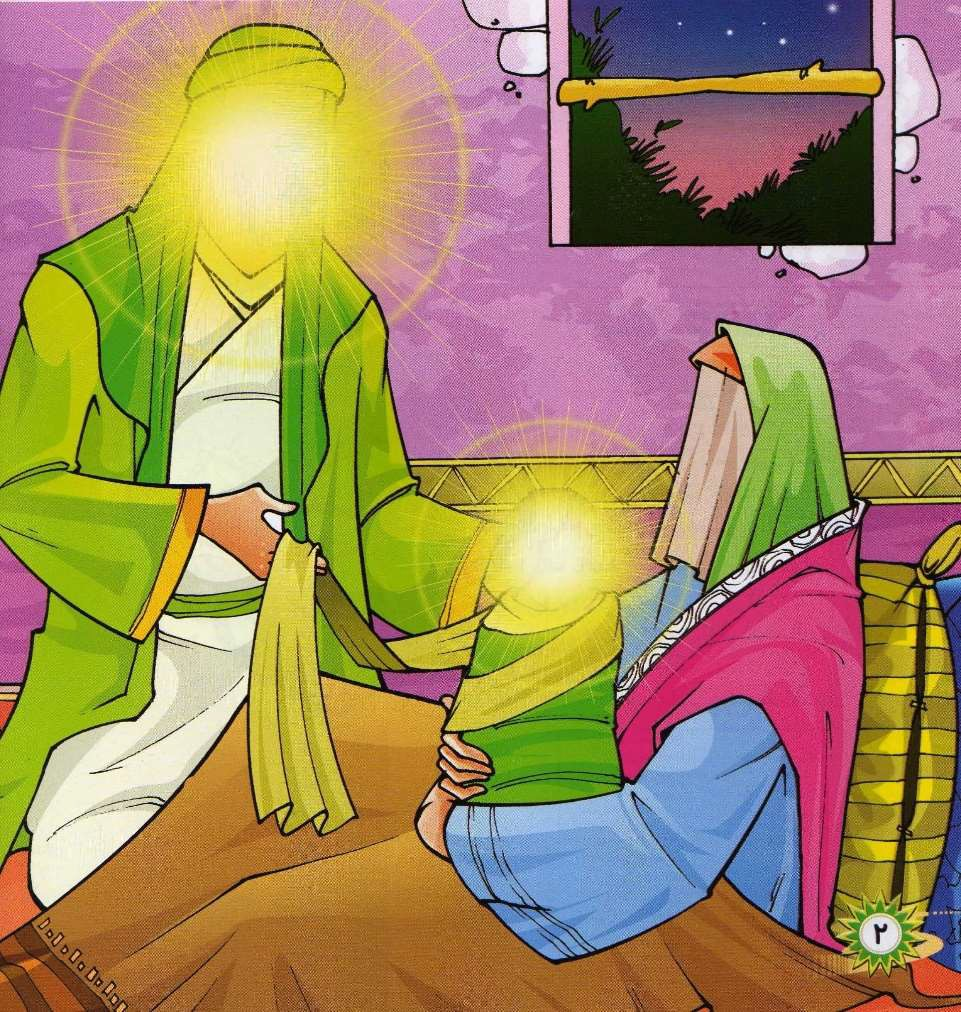
\includegraphics[width=6.3in,height=4.20208in]{media/image4.jpeg}

Selon la théologie musulmane, l'islam est la religion originelle de
l'humanité.VICTOR MOUSSA - STOCK.ADOBE.COM

\subsection{► Que dit la tradition ?}

Selon la théologie musulmane, l'islam est la religion originelle de
l'humanité.~\emph{« Tout homme est né musulman »,}~dit un hadith
attribué
au~\href{https://www.la-croix.com/sacralite-prophete-lislam-2020-11-06-1101123195}{\underline{prophète
Mohammed}}. L'homme est né pour adorer Dieu : certes, il a reçu une
dignité plus haute que les autres créatures, mais celle-ci est
conditionnée à sa soumission au Dieu unique. Plus un homme applique la
loi divine (\emph{charia}), plus il devient humain. Quant au « mécréant
» (\emph{kâfir}), qui refuse de suivre la charia, il se situe en quelque
sorte à un degré inférieur d'humanité.

Cette sévérité envers les non-musulmans s'appuie sur la lecture du texte
coranique qui s'est imposée à partir du IX\textsuperscript{e}~siècle,
lors de la transformation de l'islam en un empire soucieux de se
légitimer. Confortée par des hadiths rédigés à cette époque, elle
dépeint une vérité unique et non négociable. Elle insiste sur les
versets du Coran particulièrement virulents envers les polythéistes,
païens ou idolâtres, qualifiés d'\emph{« associateurs
»}~(\emph{mouchrikoun}) car ils « associent » à Dieu d'autres divinités.

Quant aux athées,~\emph{« ils appartiennent, selon la théologie
musulmane, à une catégorie de mécréance encore inférieure aux
polythéistes, aux juifs et aux chrétiens »,~}explique l'islamologue
Abdessamad Belhaj, chercheur au Centre interdisciplinaire d'études de
l'islam dans le monde contemporain de l'Université catholique de
Louvain. Même si des institutions comme le Haut Conseil des oulémas du
Maroc ou la Maison de la fatwa en Égypte considèrent que les apostats ne
peuvent plus être condamnés à mort, cette peine reste appliquée dans une
dizaine de pays, comme l'Afghanistan ou
la~\href{https://www.la-croix.com/Monde/Afrique/prisons-Mauritanie-calvaire-dun-apostat-2019-09-30-1201051050}{\underline{Mauritanie}}.

\subsection{ Pourquoi juifs et chrétiens bénéficient-ils d'un statut
spécifique ?}

Selon la tradition musulmane, chrétiens et juifs font l'objet d'un
traitement différent des autres non-musulmans : ils bénéficient dans le
droit islamique d'une protection juridique particulière (\emph{dhimma})
toutefois accompagnée d'injonctions humiliantes, comme l'interdiction de
monter à cheval ou de construire des lieux de culte dépassant ceux des
musulmans.
 

\emph{« Le Coran est très ambivalent au sujet des ``gens du Livre''
»,~}rappelle
l'historien~\href{https://www.la-croix.com/Culture/Livres-et-idees/historiens-decryptent-Coran-avant-lislam-2019-11-27-1201063090}{\underline{Guillaume
Dye}}, professeur à l'Université libre de Bruxelles (1). Selon la
sourate 5, juifs et chrétiens ne doivent pas être pris pour~\emph{«
alliés »~}(5, 51) mais, quelques versets plus loin, on lit qu'ils ne
seront~\emph{« point affligés »~}(5, 69). Les chrétiens se voient
reprocher de nier l'unicité de Dieu mais du respect est exprimé pour les
prêtres et les moines, qui~\emph{« ne s'enflent pas d'orgueil ».}

Selon une théologie dite de la falsification (\emph{tahrif}), les juifs
et les chrétiens ont altéré le message transmis par leurs prophètes
respectifs (Moïse, Jésus), message qui n'était autre que l'islam. Le
Coran, lui, corrige cette déviation en transmettant fidèlement le
message révélé à un ultime prophète, Mohammed. À Médine, celui-ci aurait
signé une~\emph{« Constitution »~}disposant que les juifs, notamment,
pouvaient pratiquer leur religion en sécurité, mais ces relations se
sont rapidement détériorées.

\subsection{► Quelles pistes pour une « théologie du pluralisme » ?}

Les attentats visant des « mécréants » en terrasse à Paris, les
persécutions contre les Yézidis ou les chrétiens en Irak, sont autant de
conséquences d'une lecture littéraliste du Coran encouragée par l'essor
du salafisme saoudien à partir des années 1970. D'autres lectures ont
pourtant existé dès les premiers siècles de l'islam. Contrairement à la
doctrine sunnite traditionnelle, l'exégèse rationaliste a par exemple
conclu très tôt à une~\emph{« égalité entre tous les êtres humains, tous
étant dotés de la même raison les rendant aptes à comprendre la parole
de Dieu »,~}rappelle l'islamologue Pierre Lory, directeur d'études à
l'École pratique des hautes études (EPHE).

Pour Abdessamad Belhaj, tout l'enjeu est aujourd'hui de refonder le
rapport à l'altérité sur la base de l'éthique, et de\emph{~« mettre
l'homme au cœur de la théologie »}. Pour cela, certaines valeurs
présentes dans l'islam gagneraient à être redécouvertes, comme celles du
soin, du don et du service à l'humanité, longtemps éclipsées selon lui
par l'autorité et la loyauté à la communauté musulmane ou à la tribu.

(1) Il a codirigé avec Mohammad Ali Amir-Moezzi, Le Coran des
historiens, 2019, Éd. du Cerf, 3~408~p., 89~€.

Faudra-t-il sauver les salafistes ?

Le gouvernement français a voulu lancer en octobre 2019 une offensive
contre l'islamisme et les courants radicaux, rapidement relayée par un
emballement médiatique qui a échappé à tout contrôle. Or, l'ennemi
désigné n'a nullement été identifié selon des termes juridiques, pas
plus que ses torts. On lui reproche sa piété rigoureuse, son voile, sa
pratique du jeûne de Ramadan, sa barbe fournie, son refus de toucher les
femmes, ce qui le rapproche dangereusement de n'importe quel fidèle
conservateur.

L'offensive vise donc une manière de concevoir la piété musulmane, et
nullement une qualification criminelle ou une atteinte à l'ordre public.
C'est dire que nous sommes confrontés à un « délit de sale gueule »,
lequel échappe à la tradition juridique républicaine, délit qui est
indiscernable, sans limite, extensible, mais politiquement pratique
auprès d'une opinion chauffée à blanc par les attentats et
l'immigration.

\subsection{Un engagement d'abord religieux}

Si l'islamiste ainsi décrit ressemble évidemment
au~\href{https://www.la-croix.com/Religion/Islam/Quest-salafisme-2018-10-14-1200975866}{\underline{salafiste}},
c'est oublier un peu vite que l'écrasante majorité des~\emph{salafi~}--
ceux qui sont attachés au modèle des « anciens » (les~\emph{salaf}),
c'est-à-dire les compagnons du Prophète -- se veulent quiétistes : leur
mode d'action est la prédication et l'action missionnaire
(la~\emph{da`wa}). Le salafiste souhaite d'abord vivre un islam épuré et
intégriste -- au sens d'intégral -- dans le cadre de sa famille et de sa
communauté.

Ce mouvement est distinct d'un engagement politique, de sorte que les
salafistes sont rarement liés aux Frères musulmans, qui eux forment un
mouvement politique. Si la matrice religieuse et idéologique du
salafisme imprègne les mentalités djihadistes, elle ne se confond pas
avec celles-ci, ni dans la pensée, ni dans les faits. La radicalisation
concerne donc à des degrés différents et sous des formes incomparables
les sympathisants du salafisme et les partisans du djihadisme de Daech.
Les premiers ont un engagement d'abord religieux, tandis que les autres
sont mus à la fois par la volonté de puissance, des facteurs politiques,
sociaux et religieux.

\subsection{L'autodidacte de l'islam présente plus de risques que le
salafiste}

L'hostilité des salafistes envers les courants djihadistes a été prouvée
à de nombreuses reprises par des déclarations publiques et surtout en
fournissant du renseignement de qualité auprès des services de police.
Le meilleur ennemi du terroriste est souvent le~\emph{salafi}, et
l'autodidacte de l'islam présente plus de risques que le salafiste.

En outre, le salafisme n'a pas été désavoué par les représentants du
culte musulman pour la simple raison que ce courant n'est pas une
idéologie : il faudrait donc lui enlever son~\emph{isme}~final et
l'appeler, selon la tradition religieuse, la~\emph{salafiya~}; il s'agit
d'un vieux courant légitime de l'islam, qui a fourni des générations
d'imams et de lettrés attachés au sens littéral du Coran et de la Sunna.

\subsection{Un « écosystème » étroit mais rassurant}

Il est évident que le salafisme représente une alternative culturelle et
sociale au modèle français, modèle égalitaire, inclusif, ouvert (au
moins en théorie). Les quelques salafi que j'ai connus -- des convertis
à 25 ou 30 \% d'entre eux -- vivaient dans un étroit triangle
géographique. Parce qu'ils souhaitent faire les cinq prières à leur
heure, sans les décaler, et ce dans une salle de prière, ils sont
contraints de vivre et de travailler non loin d'une mosquée. Ils passent
ainsi de leur habitation au lieu de travail et à la salle de prière,
lesquels se situent nécessairement dans un « écosystème » étroit mais
rassurant. Ils ne peuvent guère être exigeants sur le plan
professionnel.

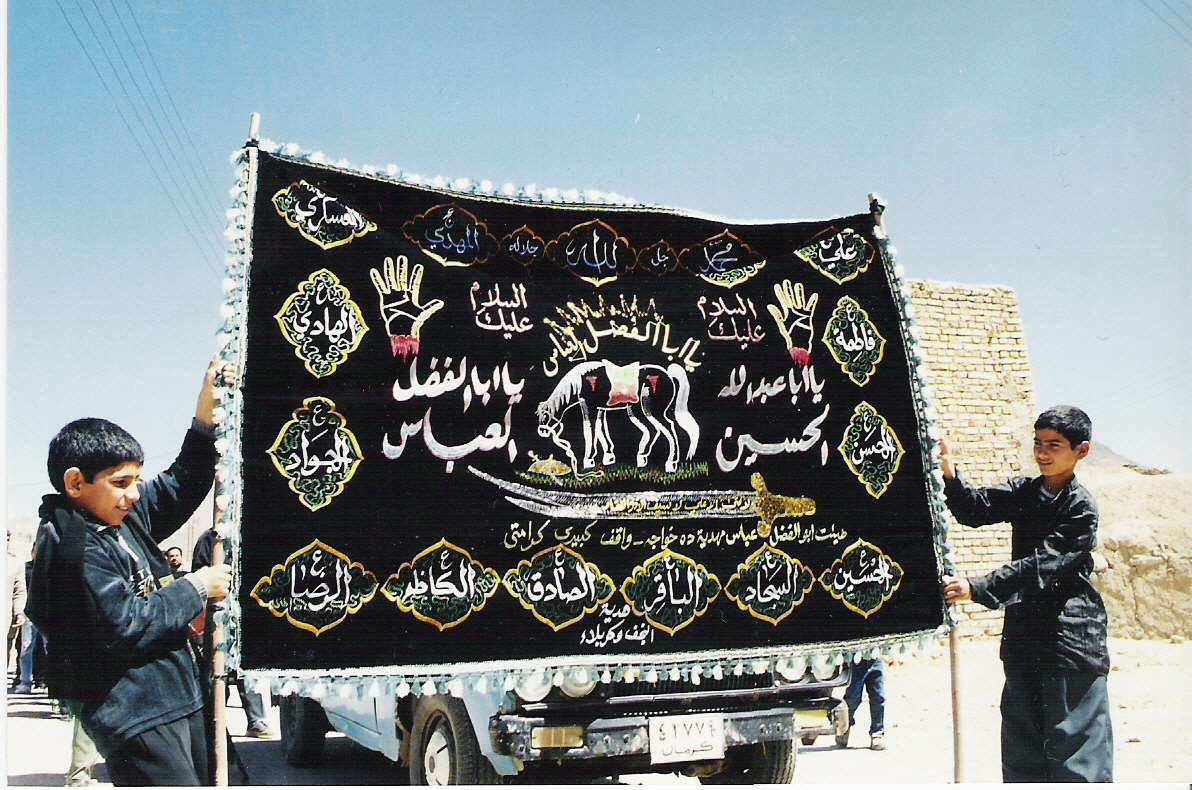
\includegraphics[width=1.97917in,height=1.40972in]{media/image6.jpeg}

\href{https://www.la-croix.com/Religion/Le-Coran-peut-etre-interprete-2021-01-25-1201136852}{Le
Coran peut-il être interprété ?}

Le salafisme, qui représente au moins 40 000 individus, est socialement
dangereux car il impose l'auto-ségrégation, le refus des contacts avec «
ceux qui n'en sont pas ». C'est la raison pour laquelle les spécialistes
des questions de sécurité se refusent à les impliquer dans la lutte
contre le djihadisme. Salafistes et terroristes participeraient à une
même matrice intellectuelle, celle du bien contre le mal, une sorte de
vision sectaire du monde. La différence vient du rapport à la violence :
assumé chez les djihadistes, rejeté chez les salafistes. Leur
fondamentalisme présente l'avantage d'une certaine forme de morale : à
Sartrouville les quartiers salafisés ont vu s'effondrer la toxicomanie
et la délinquance, avec le soutien de la mairie.

\subsection{Confondre l'approche culturelle avec la lutte contre le
terrorisme}

Ces courants ne peuvent être incriminés sur le plan sécuritaire. On
confond donc l'approche culturelle avec la lutte contre le terrorisme. À
moins de changer tout le droit européen, la première doit être menée par
l'éducation, la philosophie, la raison, le débat ; quant à la seconde
elle doit s'appuyer sur le droit et sur des qualifications pénales, et
non sur de vagues impressions de « radicalisation », notion qui n'a
toujours pas été appréhendée de façon rigoureuse en termes sociologiques
et psychologiques.

Comme la guerre d'Algérie nous l'enseigne, une telle manière de
concevoir l'action politique va aboutir à l'effet inverse de celui
recherché : le renforcement de la méfiance collective, le repli
communautaire du côté musulman, l'action violente du côté des « anti »,
et, finalement, la fragmentation sociale et l'insécurité.

\subsection{Islam : les fumées de la radicalisation}

Olivier Hanne, médiéviste (université de Poitiers), chercheur en
islamologie, estime qu'il est très difficile de définir le parcours type
d'une personne radicalisée. Le dernier de trois articles consacrés à
l'islam en France. 
 

Qui parle d'islam aujourd'hui pense aussitôt à la radicalisation. En
2015, on estimait entre 8 000 et 10 000 le nombre de Français
radicalisés. Leurs profils sont si variés qu'il est difficile de donner
des catégories fixes : les mineurs représentent 25 \% des cas, les
femmes 27 \%, les personnes signalées sont plutôt jeunes (entre 16 et 30
ans), leur niveau scolaire est généralement faible, même si l'on
rencontre des diplômés.

La plupart travaillent. Internet représente pour tous ces individus un
passage obligé, même s'il se concrétise différemment : terrain initial
de la radicalisation, facteur de renforcement ou vecteur unique de
l'expression radicale, le partage des contenus djihadistes sur Internet
n'a pas du tout la même fonction chez une adolescente connectée, un
salafiste convaincu et un combattant expérimenté déjà parti en Syrie.

\subsection{Les autorités font feu de tout bois}

De toute évidence, l'attraction pour la radicalité religieuse n'est pas
nécessairement liée à un phénomène de rupture sociale. Les failles de la
société contemporaine (éclatement des familles, déclin des autorités et
des idéologies, chômage, ghettoïsation) créent un terreau facilitateur,
mais nullement déterminant. La frustration individuelle alimente le
recours à des convictions extrêmes, voire le passage à l'acte
terroriste, mais n'est qu'un facteur parmi tant d'autres.

Les autorités font feu de tout bois pour tenter de faire face à une
radicalisation multiforme. En avril 2015, le premier ministre français,
Manuel Valls, annonçait l'ouverture d'une dizaine de centres de
prévention de la radicalisation, dont la plupart furent un échec. Des
sites Internet officiels sont créés et proposent des fiches techniques
contre la radicalisation et le terrorisme, dont le contenu est souvent
simple, voire binaire. Ainsi sur le site
français~\emph{stop-djihadisme.gouv.fr}, un bandeau intitulé «
Radicalisation djihadiste, les premiers signes qui peuvent alerter »
énonce pêle-mêle : « ils se méfient des anciens amis qu'ils considèrent
maintenant comme des impurs » ; « ils changent brutalement leurs
habitudes alimentaires » ; « ils arrêtent d'écouter de la musique car
elle les détourne de leur mission » ; « ils ne regardent plus la
télévision et ne vont plus au cinéma ». Autant de signes extérieurs qui
se rapprochent de l'adolescente anorexique\ldots{} L'efficacité de ces
dispositifs a d'ailleurs été très contestée dès 2015.

\subsection{L'État, tenté d'être omniprésent}

Toute l'entreprise de déradicalisation définit en creux le modèle
positif occidental : monde de loisirs, de consommation, d'épanouissement
personnel et professionnel. Le vocabulaire de la radicalisation masque
le rejet de ce modèle culturel. Et les pouvoirs publics d'hésiter à
appeler leur objectif par son vrai nom : le reconditionnement mental.

Le danger de la déradicalisation se situe dans l'élargissement des
intrusions de l'État : en voulant réinsérer, l'État pénètre dans
l'intimité des individus afin de redéfinir le religieux et lui redonner
une place acceptable. Or, l'État a-t-il compétence pour définir ce
qu'est l'islam, le « bon » islam ? Ne sachant cerner la menace, l'État
est tenté d'être omniprésent, sans en avoir la capacité légale. La
déradicalisation pourrait relever de la posture intellectuelle.

Le problème vient sans doute des hésitations du vocabulaire. Car,
après-tout, qu'est-ce que la radicalisation ? Au
XIX\textsuperscript{e}~le mot anglais~\emph{radical}~était employé pour
désigner les partis politiques britanniques exigeant une réforme
démocratique libérale. Transféré tel quel en France, on l'appliqua aux
partis de gauche, laïques et libéraux qui voulaient réformer la société.

\subsection{Réactions épidermiques}

Le verbe « radicaliser » fut employé régulièrement dans les années
1960-1970 dans une acception politique avec l'idée de « devenir plus
intransigeant, se durcir » ou « plus extrême ». Le premier sens était
donc politique et pas nécessairement négatif. Se déradicaliser était un
synonyme pour « se compromettre ». Appliqué à l'islamisme, le verbe
impose une redéfinition complète des termes : à partir de quand
juge-t-on l'islam intransigeant ou extrême ? par rapport à quelle norme
? à quelle moyenne ?

Les réactions épidermiques qui ont suivi le meurtre de l'enseignant de
Conflans-Sainte-Honorine en octobre 2020 sont tristement révélatrices :
les imams doivent s'exprimer ! les musulmans doivent désavouer le
terrorisme et faire allégeance à la France ! Mais quand ils le font,
c'est encore insuffisant, déloyal et mensonger. Le gouvernement proposa
même qu'ils prient pour la République au cours de la prière collective
du vendredi. Nos références sur la question religieuse restent
tragiquement celles de la Révolution française : comme il y eut les «
prêtres jureurs », adhérant à la loi, contre les « prêtres réfractaires
», obstinés dans leur obéissance à Rome, de la même façon il nous faut
des « imams jureurs », intimement républicains. L'État se retrouve donc
juge des reins et des cœurs.

%\bibliography{Theo}
%\bibliographystyle{siam}
\printbibliography

\listoftheorems[ignoreall,show={Def}]
Les courants contemporains de l’islam Glossaire général

\mn{Vérifier les termes}

bid‘a : innovation ; pratique « déviante ».

da‘wa : invitation ; prédication – appel à la conversion (dans les deux sens).

fasiq : pécheur ; mauvais musulman.

fiqh : compréhension ; corpus du droit musulman.

fitna: discorde, querelle ; conflit interne au monde musulman.

hadith : récit d’un dire ou faire du Prophète, rapporté par ses compagnons.

hajj : pèlerinage annuel à La Mecque.

hijra (héjire) : « exode » - départ de Mahomet pour Médine (622).

‘ibadat : culte ; partie du droit traitant du culte.

ijma‘ : consensus ; consensus des ulama sur un point de droit.

ijtihad : effort ; effort d’interprétation du Coran.

imam : chef suprême de la communauté musulmane ; successeur du Prophète, utilisé communément par les chiites pour Ali et ses descendants.

islah : réforme.

isnad : chaîne ; chaîne de transmission des hadiths.

jihad : lutte ; soit intérieure, contre ses propres faiblesses ; soit extérieure, contre les ennemis de la communauté musulmane.

ka‘aba : monument cubique noir situé au centre de la grande mosquée de La Mecque ; selon les musulmans, désigne l’emplacement du premier autel élevé par Abraham pour le Dieu unique. Point vers lequel se dirigent les musulmans pour prier.

kafir : infidèle, mécréant

khalifa (calife) : successeur, représentant ; successeur du Prophète et chef de la communauté musulmane (sunnisme).

madrasa : école ; lieu où est assuré la transmission du savoir religieux.

mihrab : niche indiquant la direction de La Mecque dans une mosquée.
 
mu‘amalat : relations ; partie du droit traitant des relations humaines.

qibla : orientation de la prière rituelle (salat), correspondant à la direction de La Mecque.

qiyas : raisonnement par analogie (domaine du droit)

salat : prière rituelle.

seyyed : prince, chef ; descendant du Prophète par Hossein ou Hassan, fils d’Ali.

shari‘a : sentier, voie ; loi divine.

sheykh (cheykh) : vieil homme ; chef d’une tribu ; chef religieux ; personne à la tête d’une congrégation soufie, ayant la capacité de guider ses disciples.

shirk : associationnisme : fait d’adorer d’autres êtres en dehors de Dieu.

shura : principe de consultation soufi : mystique musulman sourate : chapitre du Coran
sunna : coutume ; pratiques du Prophète et de la première communauté musulmane, faisant autorité pour guider le mode de vie des croyants et déterminer la loi religieuse.

tafsir : commentaire du Coran.

tajdid : renouveau (=>mujaddidi : qui renouvelle)

taqlid : imitation ; imitation stérile des anciens (par opposition à l’ijtihad).

tariqa : voie : confrérie soufie.

tawhid : unicité (divine). Dogme fondamental de l’islam.

ulama (oulémas) : terme collectif pour désigner les lettrés musulmans.

umma : peuple ou communauté ; communauté islamique dans son ensemble.

waqf : bien immobilier ou foncier dit « de-main-morte », dépendant des institutions religieuses.

zakat : aumône rituelle, obligatoire pour les croyants.

%\listoftheorems


\end{document}